% Options for packages loaded elsewhere
\PassOptionsToPackage{unicode}{hyperref}
\PassOptionsToPackage{hyphens}{url}
\PassOptionsToPackage{dvipsnames,svgnames,x11names}{xcolor}
%
\documentclass[
  letterpaper,
  DIV=11,
  numbers=noendperiod]{scrreprt}

\usepackage{amsmath,amssymb}
\usepackage{lmodern}
\usepackage{iftex}
\ifPDFTeX
  \usepackage[T1]{fontenc}
  \usepackage[utf8]{inputenc}
  \usepackage{textcomp} % provide euro and other symbols
\else % if luatex or xetex
  \usepackage{unicode-math}
  \defaultfontfeatures{Scale=MatchLowercase}
  \defaultfontfeatures[\rmfamily]{Ligatures=TeX,Scale=1}
\fi
% Use upquote if available, for straight quotes in verbatim environments
\IfFileExists{upquote.sty}{\usepackage{upquote}}{}
\IfFileExists{microtype.sty}{% use microtype if available
  \usepackage[]{microtype}
  \UseMicrotypeSet[protrusion]{basicmath} % disable protrusion for tt fonts
}{}
\makeatletter
\@ifundefined{KOMAClassName}{% if non-KOMA class
  \IfFileExists{parskip.sty}{%
    \usepackage{parskip}
  }{% else
    \setlength{\parindent}{0pt}
    \setlength{\parskip}{6pt plus 2pt minus 1pt}}
}{% if KOMA class
  \KOMAoptions{parskip=half}}
\makeatother
\usepackage{xcolor}
\setlength{\emergencystretch}{3em} % prevent overfull lines
\setcounter{secnumdepth}{5}
% Make \paragraph and \subparagraph free-standing
\ifx\paragraph\undefined\else
  \let\oldparagraph\paragraph
  \renewcommand{\paragraph}[1]{\oldparagraph{#1}\mbox{}}
\fi
\ifx\subparagraph\undefined\else
  \let\oldsubparagraph\subparagraph
  \renewcommand{\subparagraph}[1]{\oldsubparagraph{#1}\mbox{}}
\fi

\usepackage{color}
\usepackage{fancyvrb}
\newcommand{\VerbBar}{|}
\newcommand{\VERB}{\Verb[commandchars=\\\{\}]}
\DefineVerbatimEnvironment{Highlighting}{Verbatim}{commandchars=\\\{\}}
% Add ',fontsize=\small' for more characters per line
\usepackage{framed}
\definecolor{shadecolor}{RGB}{241,243,245}
\newenvironment{Shaded}{\begin{snugshade}}{\end{snugshade}}
\newcommand{\AlertTok}[1]{\textcolor[rgb]{0.68,0.00,0.00}{#1}}
\newcommand{\AnnotationTok}[1]{\textcolor[rgb]{0.37,0.37,0.37}{#1}}
\newcommand{\AttributeTok}[1]{\textcolor[rgb]{0.40,0.45,0.13}{#1}}
\newcommand{\BaseNTok}[1]{\textcolor[rgb]{0.68,0.00,0.00}{#1}}
\newcommand{\BuiltInTok}[1]{\textcolor[rgb]{0.00,0.23,0.31}{#1}}
\newcommand{\CharTok}[1]{\textcolor[rgb]{0.13,0.47,0.30}{#1}}
\newcommand{\CommentTok}[1]{\textcolor[rgb]{0.37,0.37,0.37}{#1}}
\newcommand{\CommentVarTok}[1]{\textcolor[rgb]{0.37,0.37,0.37}{\textit{#1}}}
\newcommand{\ConstantTok}[1]{\textcolor[rgb]{0.56,0.35,0.01}{#1}}
\newcommand{\ControlFlowTok}[1]{\textcolor[rgb]{0.00,0.23,0.31}{#1}}
\newcommand{\DataTypeTok}[1]{\textcolor[rgb]{0.68,0.00,0.00}{#1}}
\newcommand{\DecValTok}[1]{\textcolor[rgb]{0.68,0.00,0.00}{#1}}
\newcommand{\DocumentationTok}[1]{\textcolor[rgb]{0.37,0.37,0.37}{\textit{#1}}}
\newcommand{\ErrorTok}[1]{\textcolor[rgb]{0.68,0.00,0.00}{#1}}
\newcommand{\ExtensionTok}[1]{\textcolor[rgb]{0.00,0.23,0.31}{#1}}
\newcommand{\FloatTok}[1]{\textcolor[rgb]{0.68,0.00,0.00}{#1}}
\newcommand{\FunctionTok}[1]{\textcolor[rgb]{0.28,0.35,0.67}{#1}}
\newcommand{\ImportTok}[1]{\textcolor[rgb]{0.00,0.46,0.62}{#1}}
\newcommand{\InformationTok}[1]{\textcolor[rgb]{0.37,0.37,0.37}{#1}}
\newcommand{\KeywordTok}[1]{\textcolor[rgb]{0.00,0.23,0.31}{#1}}
\newcommand{\NormalTok}[1]{\textcolor[rgb]{0.00,0.23,0.31}{#1}}
\newcommand{\OperatorTok}[1]{\textcolor[rgb]{0.37,0.37,0.37}{#1}}
\newcommand{\OtherTok}[1]{\textcolor[rgb]{0.00,0.23,0.31}{#1}}
\newcommand{\PreprocessorTok}[1]{\textcolor[rgb]{0.68,0.00,0.00}{#1}}
\newcommand{\RegionMarkerTok}[1]{\textcolor[rgb]{0.00,0.23,0.31}{#1}}
\newcommand{\SpecialCharTok}[1]{\textcolor[rgb]{0.37,0.37,0.37}{#1}}
\newcommand{\SpecialStringTok}[1]{\textcolor[rgb]{0.13,0.47,0.30}{#1}}
\newcommand{\StringTok}[1]{\textcolor[rgb]{0.13,0.47,0.30}{#1}}
\newcommand{\VariableTok}[1]{\textcolor[rgb]{0.07,0.07,0.07}{#1}}
\newcommand{\VerbatimStringTok}[1]{\textcolor[rgb]{0.13,0.47,0.30}{#1}}
\newcommand{\WarningTok}[1]{\textcolor[rgb]{0.37,0.37,0.37}{\textit{#1}}}

\providecommand{\tightlist}{%
  \setlength{\itemsep}{0pt}\setlength{\parskip}{0pt}}\usepackage{longtable,booktabs,array}
\usepackage{calc} % for calculating minipage widths
% Correct order of tables after \paragraph or \subparagraph
\usepackage{etoolbox}
\makeatletter
\patchcmd\longtable{\par}{\if@noskipsec\mbox{}\fi\par}{}{}
\makeatother
% Allow footnotes in longtable head/foot
\IfFileExists{footnotehyper.sty}{\usepackage{footnotehyper}}{\usepackage{footnote}}
\makesavenoteenv{longtable}
\usepackage{graphicx}
\makeatletter
\def\maxwidth{\ifdim\Gin@nat@width>\linewidth\linewidth\else\Gin@nat@width\fi}
\def\maxheight{\ifdim\Gin@nat@height>\textheight\textheight\else\Gin@nat@height\fi}
\makeatother
% Scale images if necessary, so that they will not overflow the page
% margins by default, and it is still possible to overwrite the defaults
% using explicit options in \includegraphics[width, height, ...]{}
\setkeys{Gin}{width=\maxwidth,height=\maxheight,keepaspectratio}
% Set default figure placement to htbp
\makeatletter
\def\fps@figure{htbp}
\makeatother
\newlength{\cslhangindent}
\setlength{\cslhangindent}{1.5em}
\newlength{\csllabelwidth}
\setlength{\csllabelwidth}{3em}
\newlength{\cslentryspacingunit} % times entry-spacing
\setlength{\cslentryspacingunit}{\parskip}
\newenvironment{CSLReferences}[2] % #1 hanging-ident, #2 entry spacing
 {% don't indent paragraphs
  \setlength{\parindent}{0pt}
  % turn on hanging indent if param 1 is 1
  \ifodd #1
  \let\oldpar\par
  \def\par{\hangindent=\cslhangindent\oldpar}
  \fi
  % set entry spacing
  \setlength{\parskip}{#2\cslentryspacingunit}
 }%
 {}
\usepackage{calc}
\newcommand{\CSLBlock}[1]{#1\hfill\break}
\newcommand{\CSLLeftMargin}[1]{\parbox[t]{\csllabelwidth}{#1}}
\newcommand{\CSLRightInline}[1]{\parbox[t]{\linewidth - \csllabelwidth}{#1}\break}
\newcommand{\CSLIndent}[1]{\hspace{\cslhangindent}#1}

\usepackage{booktabs}
\usepackage{longtable}
\usepackage{array}
\usepackage{multirow}
\usepackage{wrapfig}
\usepackage{float}
\usepackage{colortbl}
\usepackage{pdflscape}
\usepackage{tabu}
\usepackage{threeparttable}
\usepackage{threeparttablex}
\usepackage[normalem]{ulem}
\usepackage{makecell}
\usepackage{xcolor}
\KOMAoption{captions}{tableheading}
\makeatletter
\@ifpackageloaded{tcolorbox}{}{\usepackage[many]{tcolorbox}}
\@ifpackageloaded{fontawesome5}{}{\usepackage{fontawesome5}}
\definecolor{quarto-callout-color}{HTML}{909090}
\definecolor{quarto-callout-note-color}{HTML}{0758E5}
\definecolor{quarto-callout-important-color}{HTML}{CC1914}
\definecolor{quarto-callout-warning-color}{HTML}{EB9113}
\definecolor{quarto-callout-tip-color}{HTML}{00A047}
\definecolor{quarto-callout-caution-color}{HTML}{FC5300}
\definecolor{quarto-callout-color-frame}{HTML}{acacac}
\definecolor{quarto-callout-note-color-frame}{HTML}{4582ec}
\definecolor{quarto-callout-important-color-frame}{HTML}{d9534f}
\definecolor{quarto-callout-warning-color-frame}{HTML}{f0ad4e}
\definecolor{quarto-callout-tip-color-frame}{HTML}{02b875}
\definecolor{quarto-callout-caution-color-frame}{HTML}{fd7e14}
\makeatother
\makeatletter
\makeatother
\makeatletter
\@ifpackageloaded{bookmark}{}{\usepackage{bookmark}}
\makeatother
\makeatletter
\@ifpackageloaded{caption}{}{\usepackage{caption}}
\AtBeginDocument{%
\ifdefined\contentsname
  \renewcommand*\contentsname{Table of contents}
\else
  \newcommand\contentsname{Table of contents}
\fi
\ifdefined\listfigurename
  \renewcommand*\listfigurename{List of Figures}
\else
  \newcommand\listfigurename{List of Figures}
\fi
\ifdefined\listtablename
  \renewcommand*\listtablename{List of Tables}
\else
  \newcommand\listtablename{List of Tables}
\fi
\ifdefined\figurename
  \renewcommand*\figurename{Figure}
\else
  \newcommand\figurename{Figure}
\fi
\ifdefined\tablename
  \renewcommand*\tablename{Table}
\else
  \newcommand\tablename{Table}
\fi
}
\@ifpackageloaded{float}{}{\usepackage{float}}
\floatstyle{ruled}
\@ifundefined{c@chapter}{\newfloat{codelisting}{h}{lop}}{\newfloat{codelisting}{h}{lop}[chapter]}
\floatname{codelisting}{Listing}
\newcommand*\listoflistings{\listof{codelisting}{List of Listings}}
\usepackage{amsthm}
\theoremstyle{definition}
\newtheorem{exercise}{Exercise}[chapter]
\theoremstyle{remark}
\renewcommand*{\proofname}{Proof}
\newtheorem*{remark}{Remark}
\newtheorem*{solution}{Solution}
\makeatother
\makeatletter
\@ifpackageloaded{caption}{}{\usepackage{caption}}
\@ifpackageloaded{subcaption}{}{\usepackage{subcaption}}
\makeatother
\makeatletter
\@ifpackageloaded{tcolorbox}{}{\usepackage[many]{tcolorbox}}
\makeatother
\makeatletter
\@ifundefined{shadecolor}{\definecolor{shadecolor}{rgb}{.97, .97, .97}}
\makeatother
\makeatletter
\makeatother
\ifLuaTeX
  \usepackage{selnolig}  % disable illegal ligatures
\fi
\IfFileExists{bookmark.sty}{\usepackage{bookmark}}{\usepackage{hyperref}}
\IfFileExists{xurl.sty}{\usepackage{xurl}}{} % add URL line breaks if available
\urlstyle{same} % disable monospaced font for URLs
\hypersetup{
  pdftitle={Introduction to Statistics and Data Science},
  pdfauthor={Elizabeth Tipton; Arend M Kuyper; Danielle Sass; Kaitlyn G. Fitzgerald; Adapted from ModernDive by; Chester Ismay and Albert Y. Kim},
  colorlinks=true,
  linkcolor={blue},
  filecolor={Maroon},
  citecolor={Blue},
  urlcolor={Blue},
  pdfcreator={LaTeX via pandoc}}

\title{Introduction to Statistics and Data Science}
\author{Elizabeth Tipton \and Arend M Kuyper \and Danielle
Sass \and Kaitlyn G. Fitzgerald \and Adapted from ModernDive
by \and Chester Ismay and Albert Y. Kim}
\date{2022-10-05}

\begin{document}
\maketitle
\ifdefined\Shaded\renewenvironment{Shaded}{\begin{tcolorbox}[borderline west={3pt}{0pt}{shadecolor}, enhanced, boxrule=0pt, interior hidden, sharp corners, frame hidden, breakable]}{\end{tcolorbox}}\fi

\renewcommand*\contentsname{Table of contents}
{
\hypersetup{linkcolor=}
\setcounter{tocdepth}{2}
\tableofcontents
}
\bookmarksetup{startatroot}

\hypertarget{welcome}{%
\chapter*{Welcome}\label{welcome}}
\addcontentsline{toc}{chapter}{Welcome}

This is the website for \textbf{Introduction to Statistics and Data
Science}. This book starts you down the path of learning how to think
with data using R. You'll learn the basics of how to engage, explore,
and examine many types of data arising from several contexts. Hopefully
you'll have fun and see how valuable it is to be able to critically
think with data.

\begin{tcolorbox}[enhanced jigsaw, coltitle=black, toprule=.15mm, bottomtitle=1mm, breakable, leftrule=.75mm, title=\textcolor{quarto-callout-warning-color}{\faExclamationTriangle}\hspace{0.5em}{Warning}, opacitybacktitle=0.6, colback=white, rightrule=.15mm, opacityback=0, toptitle=1mm, colbacktitle=quarto-callout-warning-color!10!white, colframe=quarto-callout-warning-color-frame, titlerule=0mm, arc=.35mm, bottomrule=.15mm, left=2mm]
Please note that this is a ``development version'' of this book for the
new design of STAT 202. Meaning this is a work in progress being edited
and updated as we go.

We would appreciate any feedback on typos and errors.
\end{tcolorbox}

This open textbook is produced with support from
\href{https://www.library.northwestern.edu/}{Northwestern University
Libraries} and \href{https://www.nualumnae.org/}{The Alumnae of
Northwestern University}.

\begin{figure}

\begin{minipage}[t]{0.50\linewidth}

{\centering 

\raisebox{-\height}{

\href{https://www.library.northwestern.edu/}{
\includegraphics{images/logos/nu-libraries.png}}

}

\caption{}

}

\end{minipage}%
%
\begin{minipage}[t]{0.50\linewidth}

{\centering 

\raisebox{-\height}{

\href{https://www.nualumnae.org/}{
\includegraphics{images/logos/alumnae_post_cent_logo.jpeg}}

}

\caption{}

}

\end{minipage}%

\end{figure}

\hypertarget{license}{%
\section*{License}\label{license}}
\addcontentsline{toc}{section}{License}

This website is (and will always be) \textbf{free to use}, and is
licensed under the
\href{https://creativecommons.org/publicdomain/zero/1.0/}{Creative
Commons Zero v1.0 Universal} License. If you'd like to give back, please
consider reporting a typo or leaving a pull request at
\href{https://github.com/NUstat/intro-stat-data-sci}{github.com/NUstat/intro-stat-data-sci}.

\bookmarksetup{startatroot}

\hypertarget{preface}{%
\chapter*{Preface}\label{preface}}
\addcontentsline{toc}{chapter}{Preface}

Help! I'm new to R and RStudio and I need to learn about them! However,
I'm completely new to coding! What do I do?

\begin{figure}

\begin{minipage}[t]{0.31\linewidth}

{\centering 

\raisebox{-\height}{

\href{https://www.r-project.org/}{
\includegraphics[width=1.01042in,height=\textheight]{images/logos/Rlogo.png}}

}

\caption{}

}

\end{minipage}%
%
\begin{minipage}[t]{0.69\linewidth}

{\centering 

\raisebox{-\height}{

\href{https://www.rstudio.com/products/rstudio/download/}{
\includegraphics[width=2.22917in,height=\textheight]{images/logos/RStudio_logo_flat.png}}

}

\caption{}

}

\end{minipage}%

\end{figure}

If you're asking yourself this question, then you've come to the right
place! Start with our ``Introduction for Students''.

\hypertarget{introduction-for-students}{%
\section*{Introduction for students}\label{introduction-for-students}}
\addcontentsline{toc}{section}{Introduction for students}

This book assumes no prerequisites: no algebra, no calculus, and no
prior programming/coding experience. This is intended to be a gentle
introduction to the practice of analyzing data and answering questions
using data the way statisticians, data scientists, data journalists, and
other researchers would.

In Figure~\ref{fig-course-flowchart} we present a flowchart of what
you'll cover in this book. You'll first get started with data in
Chapter~\ref{sec-getting-started}, where you'll learn about the
difference between R and RStudio, start coding in R, understand what R
packages are, and explore your first dataset: all domestic departure
flights from a New York City airport in 2013. Then

\begin{enumerate}
\def\labelenumi{\arabic{enumi}.}
\tightlist
\item
  \textbf{Data Exploration}: You'll assemble your data science toolbox
  using \texttt{tidyverse} packages. In particular:

  \begin{itemize}
  \tightlist
  \item
    Ch.~\ref{sec-viz}: Visualizing data via the \texttt{ggplot2}
    package.
  \item
    Ch.~\ref{sec-wrangling}: Wrangling data via the \texttt{dplyr}
    package.
  \item
    Ch.~\ref{sec-tidy}: Understanding the concept of ``tidy'' data as a
    standardized data input format for all packages in the
    \texttt{tidyverse}
  \end{itemize}
\item
  \textbf{Data Modeling}: Using these data science tools, you'll start
  performing data modeling. In particular:

  \begin{itemize}
  \tightlist
  \item
    Ch.~\ref{sec-regression}: Constructing basic regression models.
  \item
    Ch.~\ref{sec-multiple-regression}: Constructing multiple regression
    models.
  \end{itemize}
\item
  \textbf{Statistical Theory}: Now you'll learn about the role of
  randomization in making inferences and the general frameworks used to
  make inferences in statistics. In particular:

  \begin{itemize}
  \tightlist
  \item
    Ch.~\ref{sec-causality}: Randomization and causality.
  \item
    Ch.~\ref{sec-populations}: Populations and generalizability.
  \item
    Ch.~\ref{sec-sampling}: Sampling distributions.
  \end{itemize}
\item
  \textbf{Statistical Inference}: You'll learn to combine your newly
  acquired data analysis and modeling skills with statistical theory to
  make inferences. In particular:

  \begin{itemize}
  \tightlist
  \item
    Ch.~\ref{sec-confidence-int}: Building confidence intervals.
  \item
    Ch.~\ref{sec-pvalues}: Calculating p-values.
  \item
    Ch.~\ref{sec-hypothesis-tests}: Conducting hypothesis tests.
  \end{itemize}
\end{enumerate}

\begin{figure}

{\centering 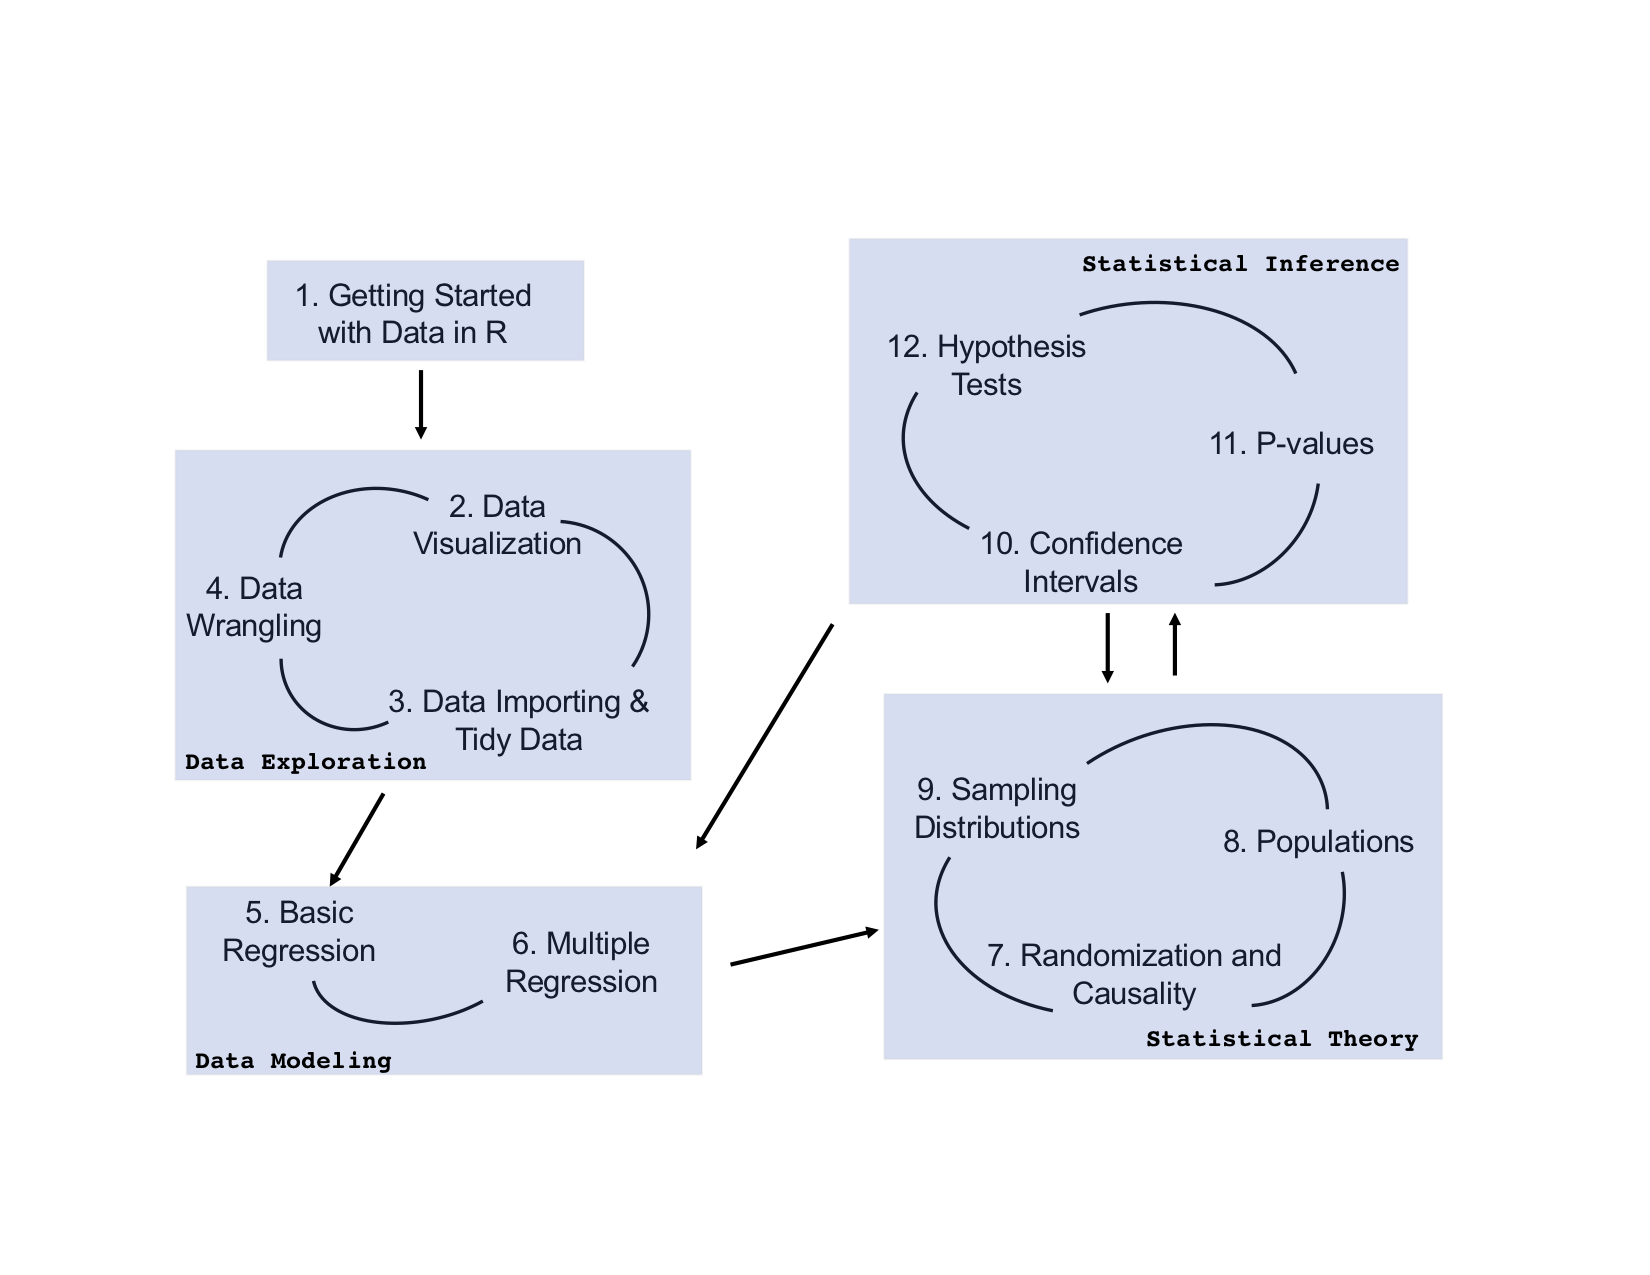
\includegraphics{images/flowcharts/STAT_202_Diagram-1.png}

}

\caption{\label{fig-course-flowchart}Course Flowchart}

\end{figure}

\hypertarget{what-you-will-learn-from-this-book}{%
\subsection*{What you will learn from this
book}\label{what-you-will-learn-from-this-book}}
\addcontentsline{toc}{subsection}{What you will learn from this book}

We hope that by the end of this book, you'll have learned

\begin{enumerate}
\def\labelenumi{\arabic{enumi}.}
\tightlist
\item
  How to use R to explore data.
\item
  How to generate research questions and hypotheses.
\item
  How to think like a statistician and the role of chance in your data.
\item
  How to answer statistical questions using tools like confidence
  intervals and hypothesis tests.
\item
  How to effectively create ``data stories'' using these tools.
\end{enumerate}

What do we mean by data stories? We mean any analysis involving data
that engages the reader in answering questions with careful visuals and
thoughtful discussion, such as
\href{http://rpubs.com/ry_lisa_elana/chicago}{How strong is the
relationship between per capita income and crime in Chicago
neighborhoods?} and
\href{https://ismayc.github.io/soc301_s2017/group_projects/group4.html}{How
many f**ks does Quentin Tarantino give (as measured by the amount of
swearing in his films)?}. Further discussions on data stories can be
found in this
\href{https://www.thinkwithgoogle.com/marketing-resources/data-measurement/tell-meaningful-stories-with-data/}{Think
With Google article}.

For other examples of data stories constructed by students like
yourselves, look at the final projects for two courses that have
previously used a version of this book:

\begin{itemize}
\tightlist
\item
  Middlebury College
  \href{https://rudeboybert.github.io/MATH116/PS/final_project/final_project_outline.html\#past_examples}{MATH
  116 Introduction to Statistical and Data Sciences} using student
  collected data.
\item
  Pacific University
  \href{https://ismayc.github.io/soc301_s2017/group-projects/index.html}{SOC
  301 Social Statistics} using data from the
  \href{https://cran.r-project.org/web/packages/fivethirtyeight/vignettes/fivethirtyeight.html}{fivethirtyeight
  R package}.
\end{itemize}

This book will help you develop your ``data science toolbox'', including
tools such as data visualization, data formatting, data wrangling, and
data modeling using regression. With these tools, you'll be able to
perform the entirety of the ``data/science pipeline'' while building
data communication skills.

In particular, this book will lean heavily on data visualization. In
today's world, we are bombarded with graphics that attempt to convey
ideas. We will explore what makes a good graphic and what the standard
ways are to convey relationships with data. You'll also see the use of
visualization to introduce concepts like mean, median, standard
deviation, distributions, etc. In general, we'll use visualization as a
way of building almost all of the ideas in this book.

To impart the statistical lessons in this book, we have intentionally
minimized the number of mathematical formulas used and instead have
focused on developing a conceptual understanding via data visualization,
statistical computing, and simulations. We hope this is a more intuitive
experience than the way statistics has traditionally been taught in the
past and how it is commonly perceived.

Finally, you'll learn the importance of literate programming. By this we
mean you'll learn how to write code that is useful not just for a
computer to execute but also for readers to understand exactly what your
analysis is doing and how you did it. This is part of a greater effort
to encourage reproducible research (see subsection \emph{Reproducible
research} for more details). Hal Abelson coined the phrase that we will
follow throughout this book:

\begin{quote}
``Programs must be written for people to read, and only incidentally for
machines to execute.''
\end{quote}

We understand that there may be challenging moments as you learn to
program. We still continue to struggle and find ourselves often using
web searches to find answers and reach out to colleagues for help. In
the long run though, we all can solve problems faster and more elegantly
via programming. We wrote this book as our way to help you get started
and you should know that there is a huge community of R users that are
always happy to help everyone along as well. This community exists in
particular on the internet on various forums and websites such as
\href{https://stackoverflow.com/}{stackoverflow.com}.

\hypertarget{datascience-pipeline}{%
\subsection*{Data/science pipeline}\label{datascience-pipeline}}
\addcontentsline{toc}{subsection}{Data/science pipeline}

You may think of statistics as just being a bunch of numbers. We
commonly hear the phrase ``statistician'' when listening to broadcasts
of sporting events. Statistics (in particular, data analysis), in
addition to describing numbers like with baseball batting averages,
plays a vital role in all of the sciences. You'll commonly hear the
phrase ``statistically significant'' thrown around in the media. You'll
see articles that say ``Science now shows that chocolate is good for
you.'' Underpinning these claims is data analysis and a theoretical
model relating the data collected in a sample to a larger population. By
the end of this book, you'll be able to better understand whether these
claims should be trusted or whether we should be wary. Inside data
analysis are many sub-fields that we will discuss throughout this book
(though not necessarily in this order):

\begin{itemize}
\tightlist
\item
  data collection
\item
  data wrangling
\item
  data visualization
\item
  data modeling
\item
  statistical inference
\item
  correlation and regression
\item
  interpretation of results
\item
  data communication/storytelling
\end{itemize}

These sub-fields are summarized in what Grolemund and Wickham term the
\href{http://r4ds.had.co.nz/explore-intro.html}{``Data/Science
Pipeline''} in Figure~\ref{fig-pipline}.

\begin{figure}

{\centering 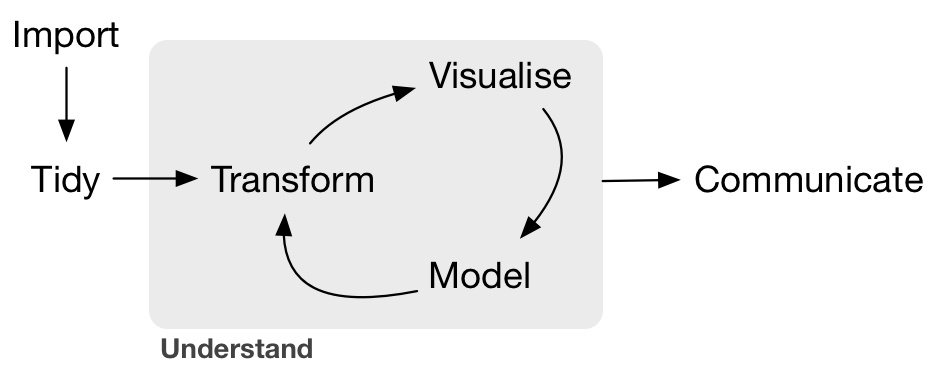
\includegraphics{images/tidy1.png}

}

\caption{\label{fig-pipline}Data/Science Pipeline}

\end{figure}

We will begin by digging into the gray \textbf{Understand} portion of
the cycle with data visualization, then with a discussion on what is
meant by tidy data and data wrangling, and then conclude by talking
about interpreting and discussing the results of our models via
\textbf{Communication}. These steps are vital to any statistical
analysis. But why should you care about statistics? ``Why did they make
me take this class?''

There's a reason so many fields require a statistics course. Scientific
knowledge grows through an understanding of statistical significance and
data analysis. You needn't be intimidated by statistics. It's not the
beast that it used to be and, paired with computation, you'll see how
reproducible research in the sciences particularly increases scientific
knowledge.

\hypertarget{reproducible-research}{%
\subsection*{Reproducible research}\label{reproducible-research}}
\addcontentsline{toc}{subsection}{Reproducible research}

\begin{quote}
``The most important tool is the \emph{mindset}, when starting, that the
end product will be reproducible.'' -- Keith Baggerly
\end{quote}

Another goal of this book is to help readers understand the importance
of reproducible analyses. The hope is to get readers into the habit of
making their analyses reproducible from the very beginning. This means
we'll be trying to help you build new habits. This will take practice
and be difficult at times. You'll see just why it is so important for
you to keep track of your code and well-document it to help yourself
later and any potential collaborators as well.

Copying and pasting results from one program into a word processor is
not the way that efficient and effective scientific research is
conducted. It's much more important for time to be spent on data
collection and data analysis and not on copying and pasting plots back
and forth across a variety of programs.

In a traditional analysis if an error was made with the original data,
we'd need to step through the entire process again: recreate the plots
and copy and paste all of the new plots and our statistical analysis
into your document. This is error prone and a frustrating use of time.
We'll see how to use R Markdown to get away from this tedious activity
so that we can spend more time doing science.

\begin{quote}
``We are talking about \emph{computational} reproducibility.'' - Yihui
Xie
\end{quote}

Reproducibility means a lot of things in terms of different scientific
fields. Are experiments conducted in a way that another researcher could
follow the steps and get similar results? In this book, we will focus on
what is known as \textbf{computational reproducibility}. This refers to
being able to pass all of one's data analysis, data-sets, and
conclusions to someone else and have them get exactly the same results
on their machine. This allows for time to be spent interpreting results
and considering assumptions instead of the more error prone way of
starting from scratch or following a list of steps that may be different
from machine to machine.

\part{Getting started}

\hypertarget{sec-getting-started}{%
\chapter{Getting Started with Data in R}\label{sec-getting-started}}

Before we can start exploring data in R, there are some key concepts to
understand first:

\begin{enumerate}
\def\labelenumi{\arabic{enumi}.}
\tightlist
\item
  What are R and RStudio?
\item
  How do I code in R?
\item
  What are R packages?
\end{enumerate}

We'll introduce these concepts in upcoming Sections~\ref{sec-r-rstudio}
- \ref{sec-packages} If you are already somewhat familiar with these
concepts, feel free to skip to Section~\ref{sec-nycflights13} where
we'll introduce our first data set: all domestic flights departing a New
York City airport in 2013. This is a dataset we will explore in depth in
this book.

\hypertarget{sec-r-rstudio}{%
\section{What are R and RStudio?}\label{sec-r-rstudio}}

For much of this book, we will assume that you are using R via RStudio.
First time users often confuse the two. At its simplest:

\begin{itemize}
\tightlist
\item
  R is like a car's engine.
\item
  RStudio is like a car's dashboard.
\end{itemize}

\begin{longtable}[]{@{}
  >{\centering\arraybackslash}p{(\columnwidth - 2\tabcolsep) * \real{0.4861}}
  >{\centering\arraybackslash}p{(\columnwidth - 2\tabcolsep) * \real{0.5139}}@{}}
\toprule()
\begin{minipage}[b]{\linewidth}\centering
R: Engine
\end{minipage} & \begin{minipage}[b]{\linewidth}\centering
RStudio: Dashboard
\end{minipage} \\
\midrule()
\endhead
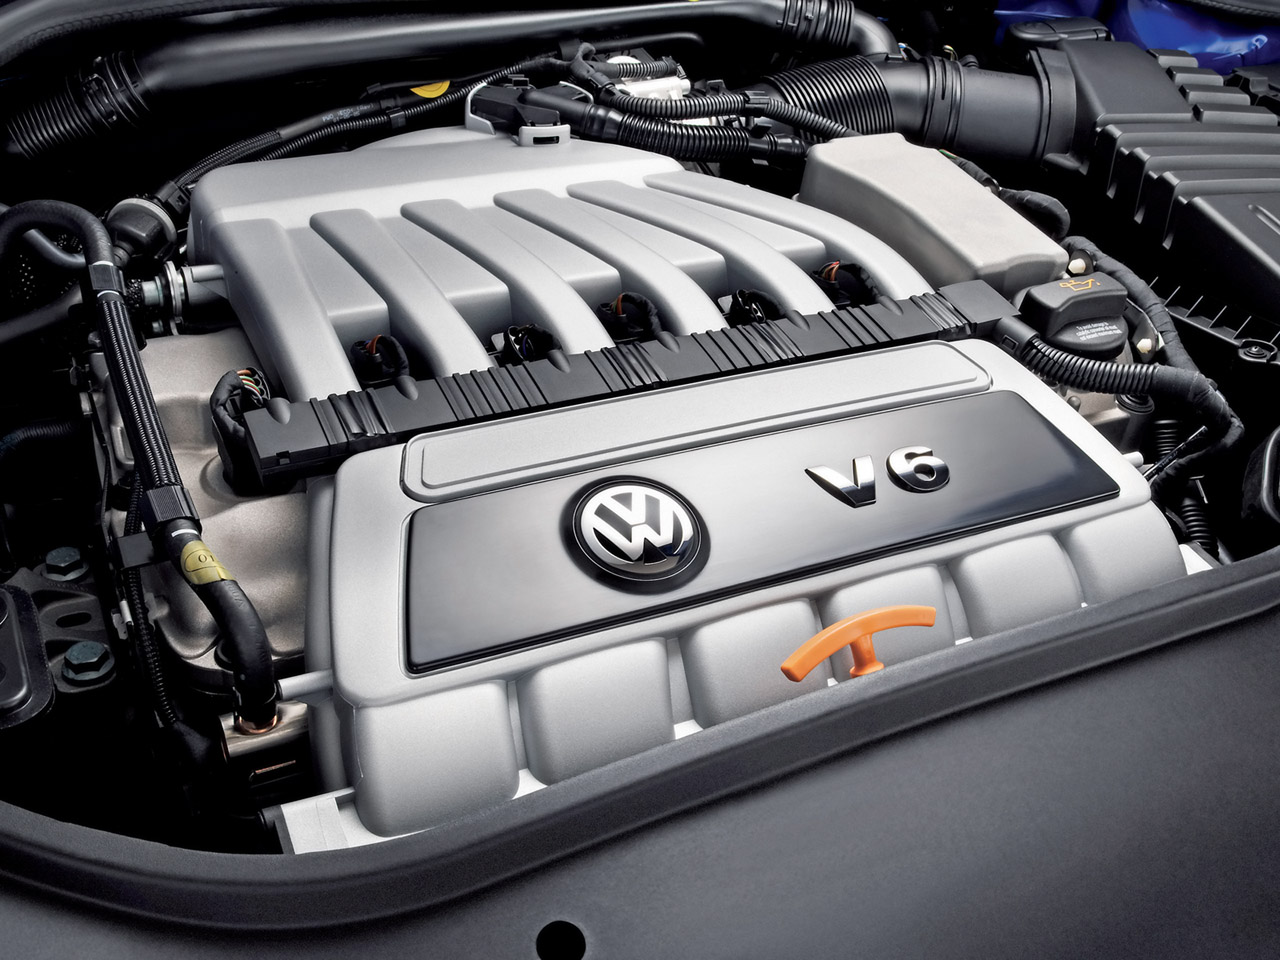
\includegraphics[width=\textwidth,height=1.7in]{images/engine.jpg} &
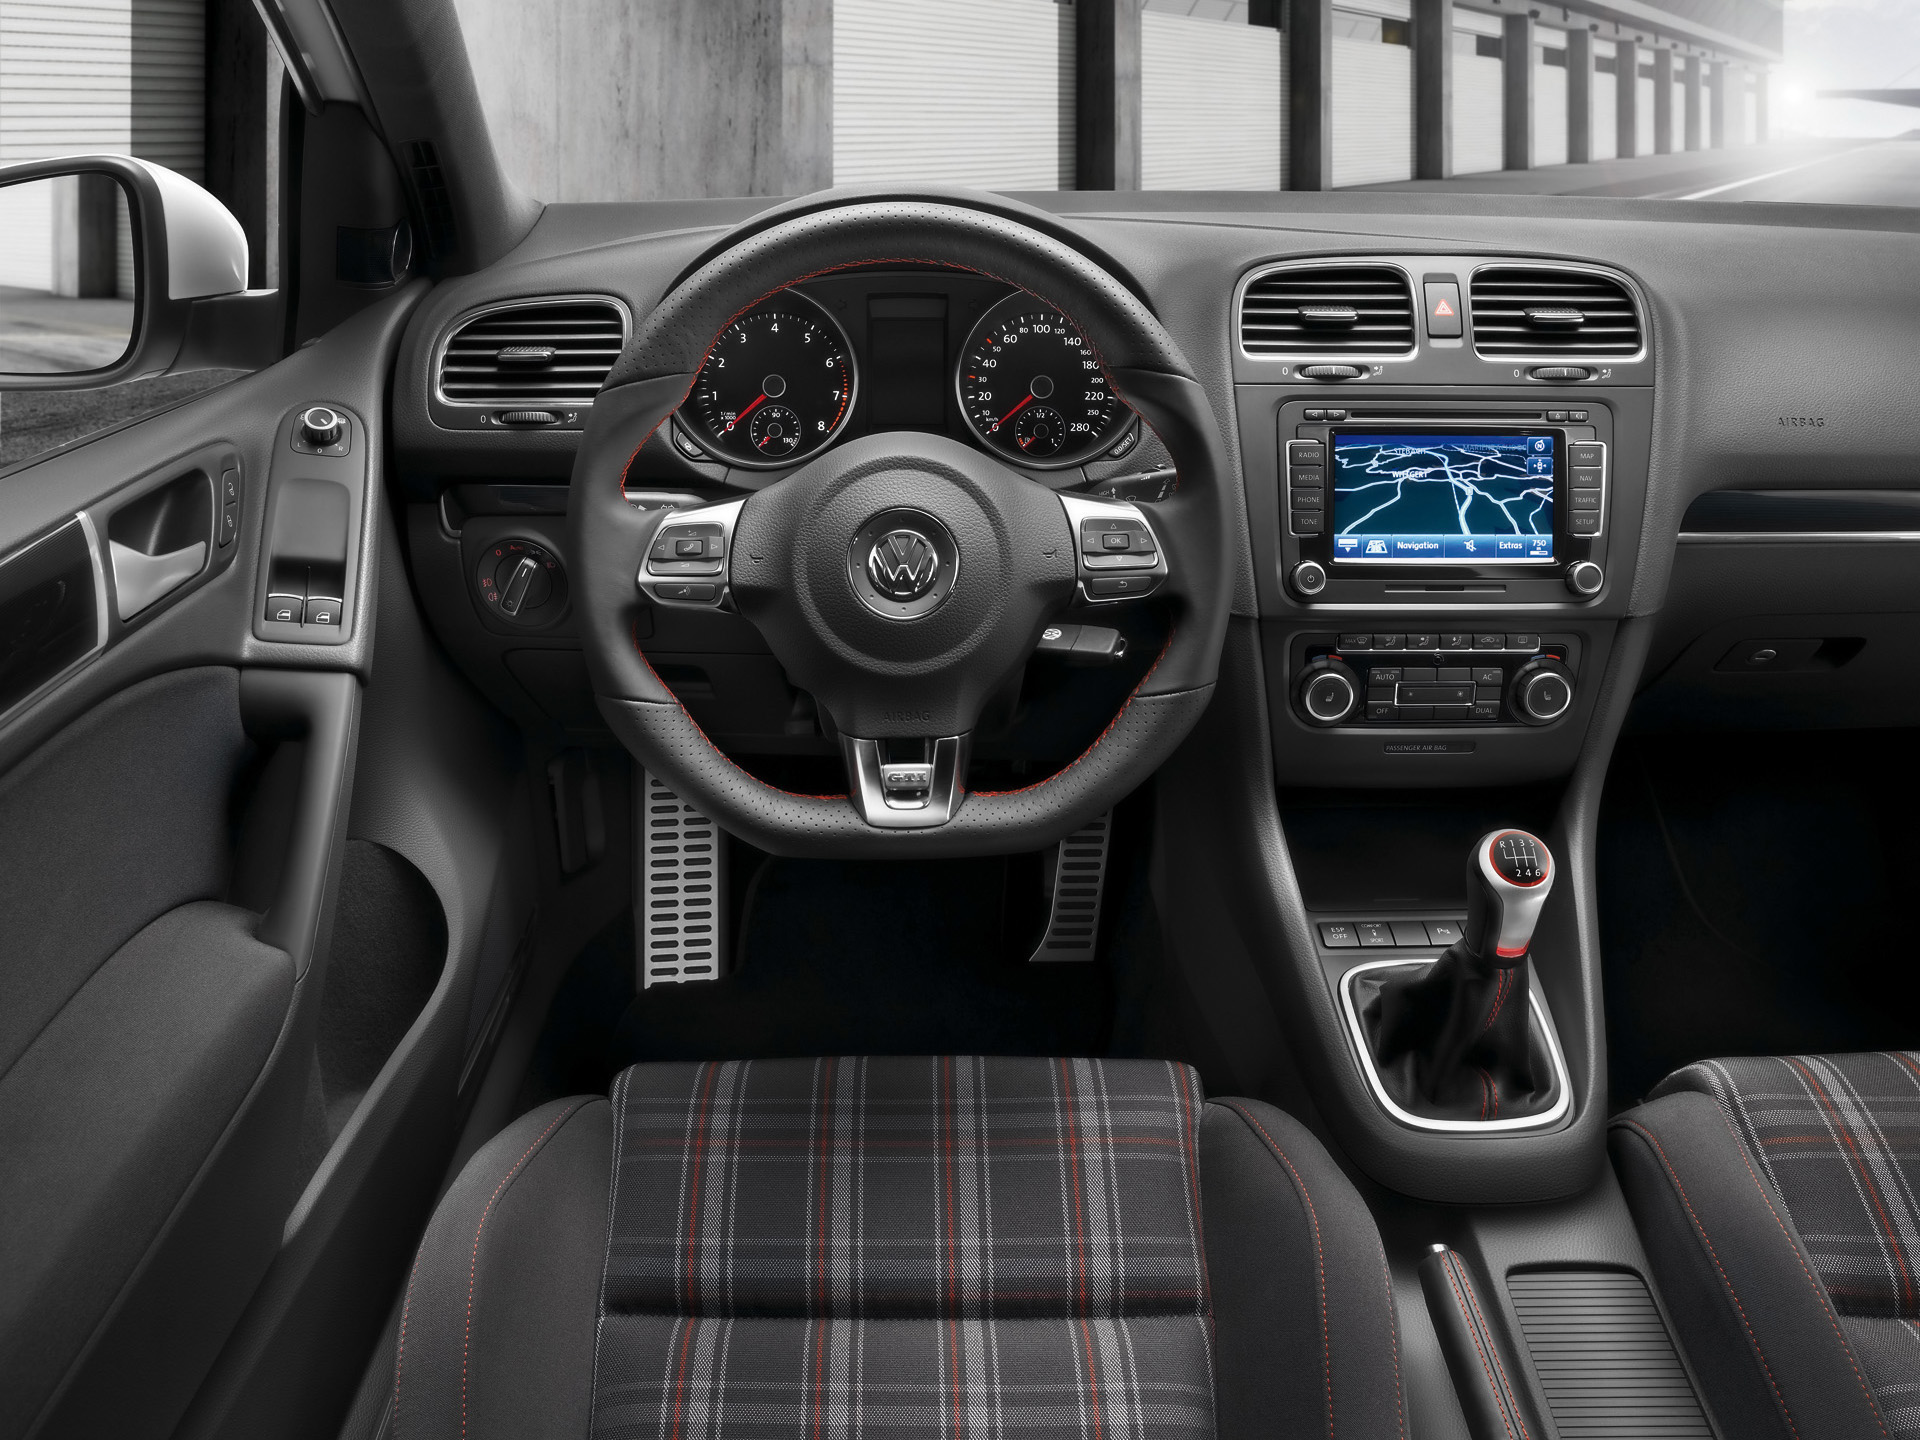
\includegraphics[width=\textwidth,height=1.7in]{images/dashboard.jpg} \\
\bottomrule()
\end{longtable}

More precisely, R is a programming language that runs computations while
RStudio is an \emph{integrated development environment (IDE)} that
provides an interface by adding many convenient features and tools. So
just as having access to a speedometer, rearview mirrors, and a
navigation system makes driving much easier, using RStudio's interface
makes using R much easier as well.

\hypertarget{using-rstudio-cloud}{%
\subsection{Using RStudio Cloud}\label{using-rstudio-cloud}}

RStudio Cloud (\url{https://rstudio.cloud}) is a hosted version of
RStudio that allows you to begin coding directly from your browser -
there is no software to install and nothing to configure on your
computer.

To begin using RStudio Cloud use the link provided by your instructor to
gain access to the classroom workspace. You will be prompted to create a
free account or log in if you have an existing account.

After you open RStudio Cloud, you should now have access to the
classroom under `Spaces' on the left hand side (in this case `STAT202').

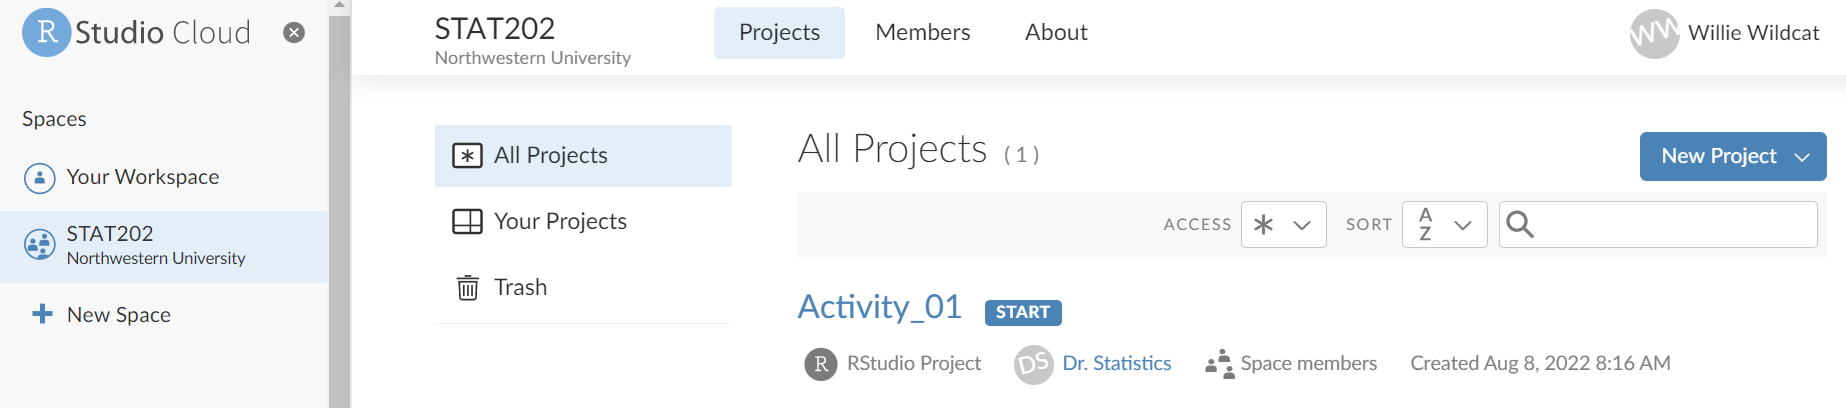
\includegraphics{images/rstudio_cloud.png}

Throughout this course you will be working on various activities. Once
the instructor has made an activity available you will click on the
classroom Workspace (STAT202) to access the available projects. To begin
working on an activity click `Start'. Once that activity project is open
navigate to the `File' pane and open the Quarto `.qmd' file.

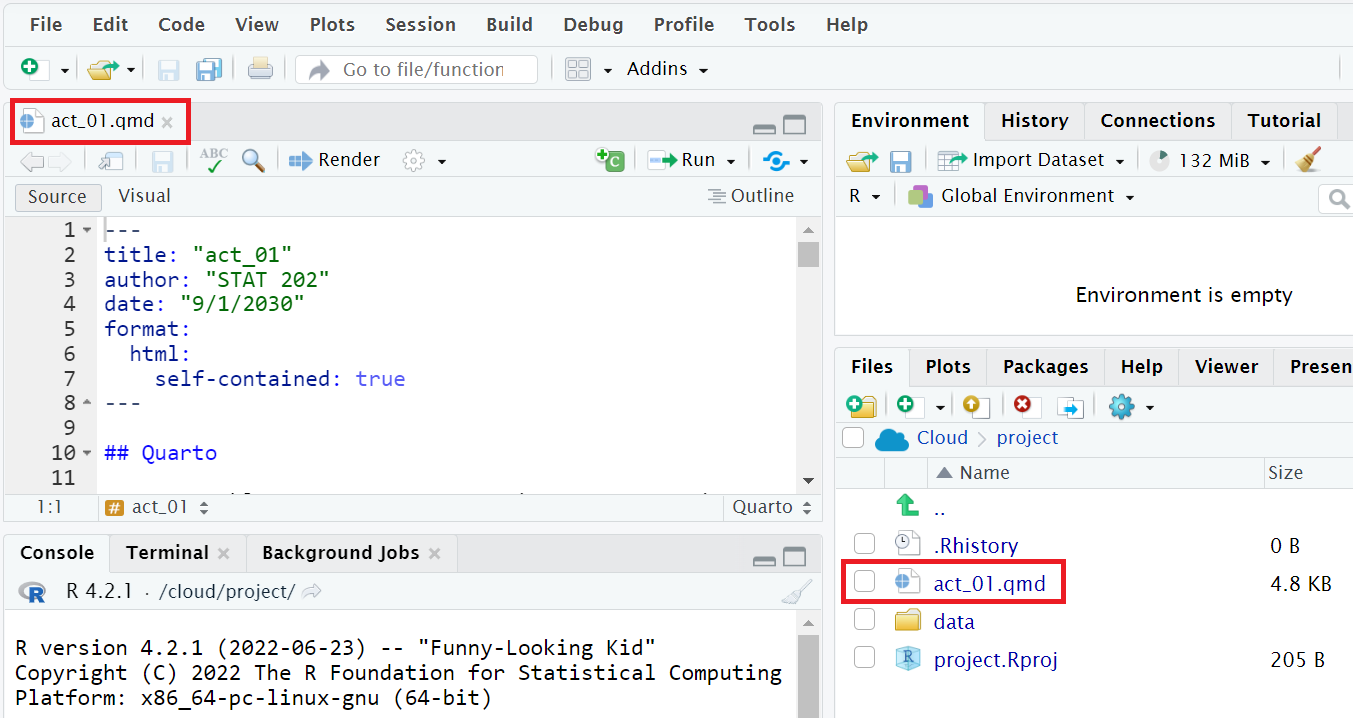
\includegraphics{images/rstudio_workspace.png}

You can use RStudio Cloud for personal use as well by creating projects
in `Your Workspace'. However, RStudio Cloud limits the number of
projects and amount of accessible time so it is recommended that you
later install the software on your own computer.

\hypertarget{installing-r-and-rstudio-on-your-personal-computer}{%
\subsection{Installing R and RStudio on your personal
computer}\label{installing-r-and-rstudio-on-your-personal-computer}}

\begin{quote}
\textbf{Note about RStudio Server or RStudio Cloud}: If your instructor
has provided you with a link and access to RStudio Server or RStudio
Cloud, then you can skip this section. We do recommend after a few
months of working on RStudio Server/Cloud that you return to these
instructions to install this software on your own computer though. You
will first need to download and install both R and RStudio (Desktop
version) on your computer. It is important that you install R first and
then install RStudio second.
\end{quote}

\begin{enumerate}
\def\labelenumi{\arabic{enumi}.}
\item
  \textbf{You must do this first:}
  \href{https://cloud.r-project.org/}{Download and install R}.

  \begin{itemize}
  \tightlist
  \item
    If you are a Windows user: Click on ``Download R for Windows'', then
    click on ``base'', then click on the Download link.
  \item
    If you are macOS user: Click on ``Download R for (Mac) OS X'', then
    under ``Latest release:'' click on R-X.X.X.pkg, where R-X.X.X is the
    version number. For example, the latest version of R as of August
    10, 2019 was R-3.6.1.
  \end{itemize}
\item
  \textbf{You must do this second:}
  \href{https://www.rstudio.com/products/rstudio/download/}{Download and
  install RStudio}.

  \begin{itemize}
  \tightlist
  \item
    Scroll down to ``Installers for Supported Platforms'' near the
    bottom of the page.
  \item
    Click on the download link corresponding to your computer's
    operating system.
  \end{itemize}
\end{enumerate}

\hypertarget{using-r-via-rstudio}{%
\subsection{Using R via RStudio}\label{using-r-via-rstudio}}

Recall our car analogy from above. Much as we don't drive a car by
interacting directly with the engine but rather by interacting with
elements on the car's dashboard, we won't be using R directly but rather
we will use RStudio's interface. After you install R and RStudio on your
computer, you'll have two new programs AKA applications you can open. We
will always work in RStudio and not R. In other words:

\begin{longtable}[]{@{}
  >{\centering\arraybackslash}p{(\columnwidth - 2\tabcolsep) * \real{0.4583}}
  >{\centering\arraybackslash}p{(\columnwidth - 2\tabcolsep) * \real{0.5417}}@{}}
\toprule()
\begin{minipage}[b]{\linewidth}\centering
R: Do not open this
\end{minipage} & \begin{minipage}[b]{\linewidth}\centering
RStudio: Open this
\end{minipage} \\
\midrule()
\endhead

\includegraphics[width=\textwidth,height=0.78125in]{images/logos/Rlogo.png}
&

\includegraphics[width=0.88542in,height=\textheight]{images/logos/rstudio-square-logo.png} \\
\bottomrule()
\end{longtable}

After you open RStudio, you should see the following:

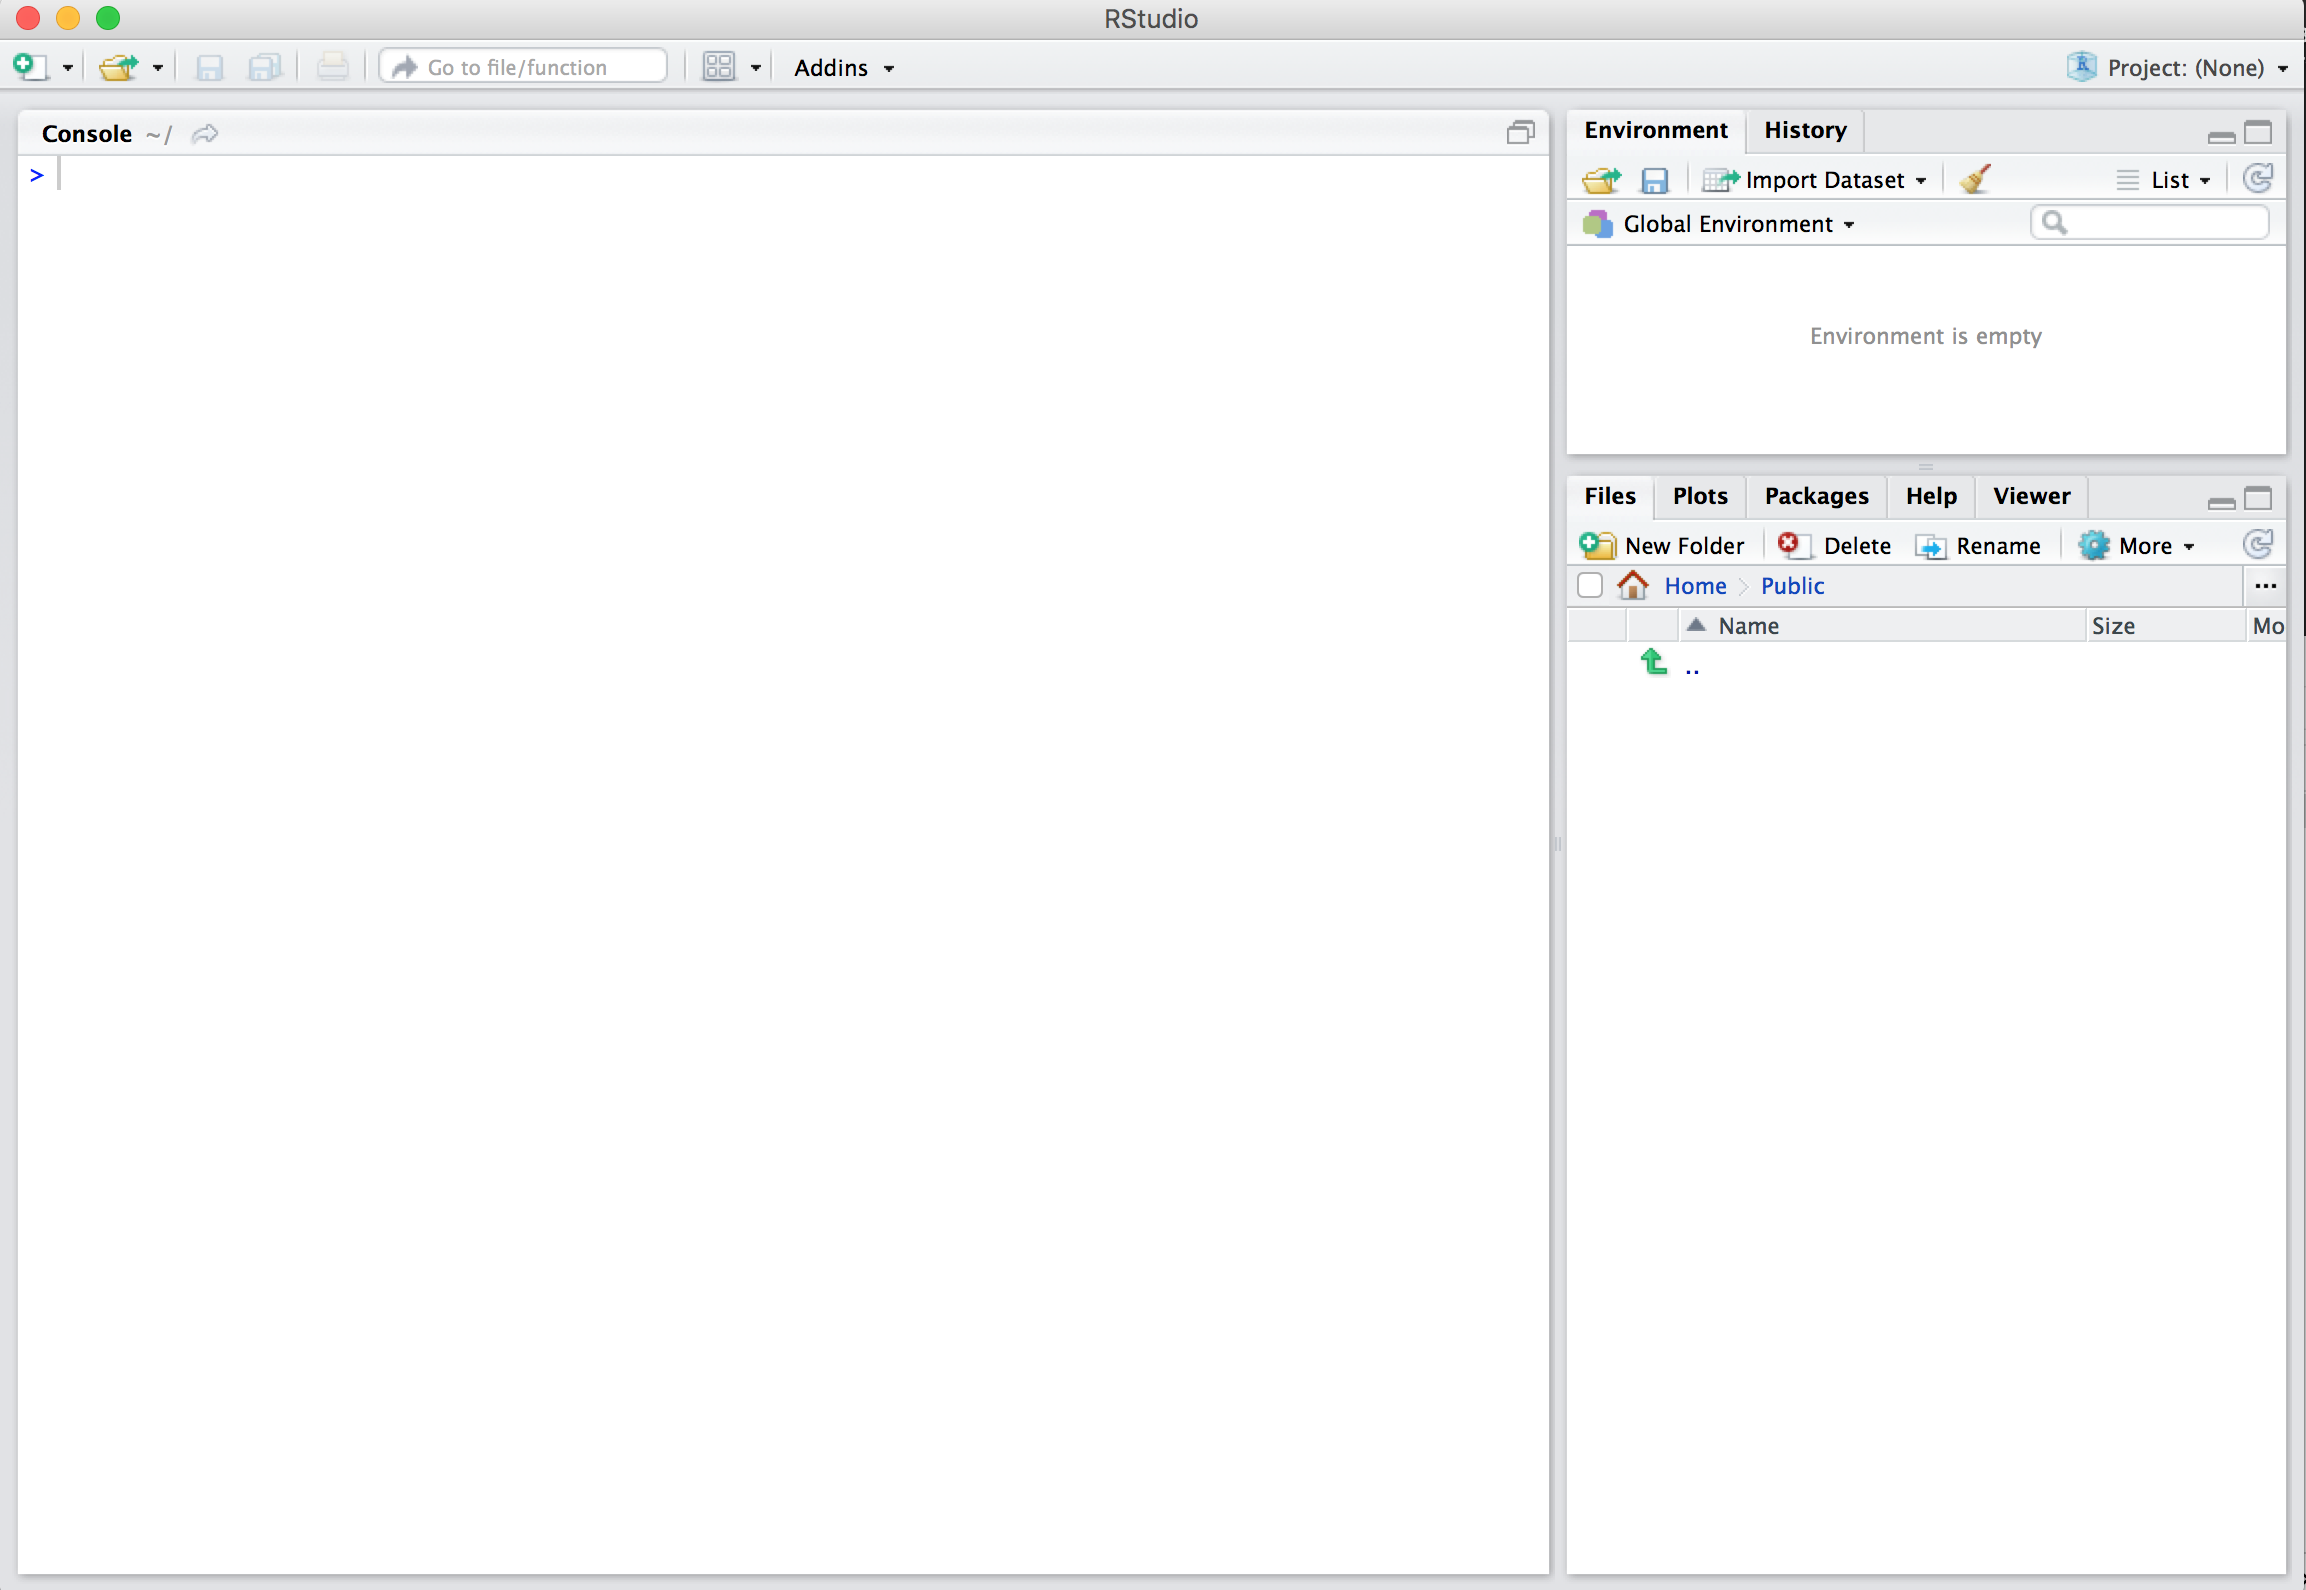
\includegraphics{images/rstudio.png}

Note the three panes, which are three panels dividing the screen: The
\emph{Console pane}, the \emph{Files pane}, and the \emph{Environment
pane}. Over the course of this chapter, you'll come to learn what
purpose each of these panes serve.

\hypertarget{sec-code}{%
\section{How do I code in R?}\label{sec-code}}

Now that you're set up with R and RStudio, you are probably asking
yourself ``OK. Now how do I use R?'' The first thing to note as that
unlike other statistical software programs like Excel, STATA, or SAS
that provide \href{https://en.wikipedia.org/wiki/Point_and_click}{point
and click} interfaces, R is an
\href{https://en.wikipedia.org/wiki/Interpreted_language}{interpreted
language}, meaning you have to enter in R commands written in R code. In
other words, you have to code/program in R. Note that we'll use the
terms ``coding'' and ``programming'' interchangeably in this book.

While it is not required to be a seasoned coder/computer programmer to
use R, there is still a set of basic programming concepts that R users
need to understand. Consequently, while this book is not a book on
programming, you will still learn just enough of these basic programming
concepts needed to explore and analyze data effectively.

\hypertarget{creating-your-first-quarto-document}{%
\subsection{Creating your first Quarto
document}\label{creating-your-first-quarto-document}}

Quarto allows you to easily create a document which combines your code,
the results from your code, as well as any text that accompanies the
analysis. To create a new Quarto file, in RStudio select
File\textgreater New File\textgreater Quarto Document. Then, you will
see a window pop-up titled \emph{New Quarto Document}. Here, you specify
the type of file you wish to create. HTML is generally the recommended
document type since it does not have traditional \emph{page} separators
like PDF and Word do. You can also choose a title and author for your
document using their respective fields. Finally, select \emph{Create} to
create your new Quarto file. You will see it appear as a tab in your
RStudio session. Click the \emph{save icon} to save your new document.

The following is an example of a Quarto document:

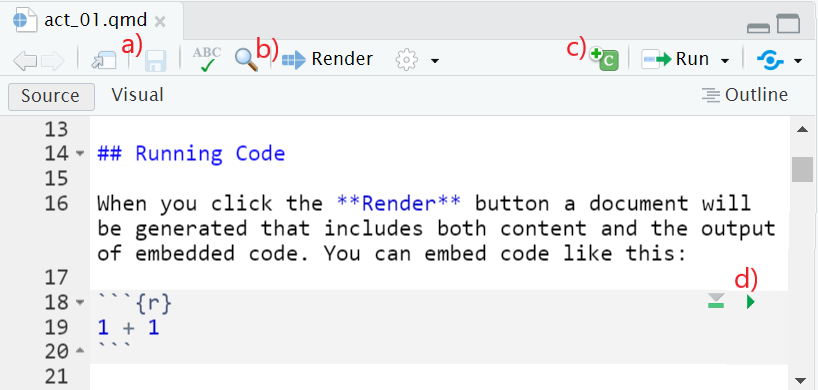
\includegraphics{images/quarto_example.png}

\begin{enumerate}
\def\labelenumi{\alph{enumi})}
\tightlist
\item
  Save your document.
\item
  Click \emph{Render} to compile your Quarto document into the file type
  that you specified. The file will be saved in your \emph{Files pane}.
  This will also save your document.
\item
  Insert a new code chunk in your document where the cursor is located.
  You will often have many code chunks in your document.
\item
  Run the current code chunk.
\end{enumerate}

When you create your Quarto file and \emph{Render} it into a document,
the chunks are run in order and any output from them is shown in the
document, in the order and location that their respective chunk appears.
Sometimes you may wish to type code or analyze data without it printing
in the document. If that is the case, you type the code in the
\emph{Console} rather than in the \emph{.qmd} file.

While you read through this book, it will be helpful to have a Quarto
document open so you can copy code provided and paste it into a code
chunk to run.

\hypertarget{sec-programming-concepts}{%
\subsection{Basic programming concepts and
terminology}\label{sec-programming-concepts}}

We now introduce some basic programming concepts and terminology.
Instead of asking you to learn all these concepts and terminology right
now, we'll guide you so that you'll ``learn by doing.'' Note that in
this book we will always use a different font to distinguish regular
text from \texttt{computer\_code}. The best way to master these topics
is, in our opinions, ``learning by doing'' and lots of repetition.

\begin{itemize}
\item
  Basics:

  \begin{itemize}
  \tightlist
  \item
    \emph{Console}: Where you enter in commands. \index{console}
  \item
    \emph{Running code}: The act of telling R to perform an action by
    giving it commands in the console.
  \item
    \emph{Objects}: Where values are saved in R. In order to do useful
    and interesting things in R, we will want to \emph{assign} a name to
    an object. For example we could do the following assignments:
    \texttt{x\ \textless{}-\ 44\ -\ 20} and
    \texttt{three\ \textless{}-\ 3}. This would allow us to run
    \texttt{x\ +\ three} which would return \texttt{27}.
  \item
    \emph{Data types}: Integers, doubles/numerics, logicals, and
    characters.
  \end{itemize}
\end{itemize}

In RStudio try typing the following code into the console or code chunk.

\begin{Shaded}
\begin{Highlighting}[]
\NormalTok{x }\OtherTok{\textless{}{-}} \DecValTok{44{-}20}
\NormalTok{three }\OtherTok{\textless{}{-}} \DecValTok{3}
\NormalTok{x}\SpecialCharTok{+}\NormalTok{three}
\end{Highlighting}
\end{Shaded}

\begin{verbatim}
[1] 27
\end{verbatim}

You should see \texttt{x} and \texttt{three} appear as stored objects in
the \emph{Environment} pane. Anything you store in the
\emph{Environment} pane can be referenced and used later. R can also be
used as a calculator, notice how it evaluates \texttt{x+three}.

\begin{itemize}
\item
  \emph{Vectors}: A series of values. These are created using the
  \texttt{c()} function, where \texttt{c()} stands for ``combine'' or
  ``concatenate''. For example: \texttt{c(6,\ 11,\ 13,\ 31,\ 90,\ 92)}.
\item
  \emph{Factors}: \emph{Categorical data} are represented in R as
  factors.
\item
  \emph{Data frames}: Data frames are like rectangular spreadsheets:
  they are representations of datasets in R where the rows correspond to
  \emph{observations} and the columns correspond to \emph{variables}
  that describe the observations. \index{data frames} We'll cover data
  frames later in Section~\ref{sec-nycflights13}.
\item
  \emph{Conditionals}:

  \begin{itemize}
  \tightlist
  \item
    Testing for equality in R using \texttt{==} (and not \texttt{=}
    which is typically used for assignment). Ex: \texttt{2\ +\ 1\ ==\ 3}
    compares \texttt{2\ +\ 1} to \texttt{3} and is correct R code, while
    \texttt{2\ +\ 1\ =\ 3} will return an error.
  \item
    Boolean algebra: \texttt{TRUE/FALSE} statements and mathematical
    operators such as \texttt{\textless{}} (less than),
    \texttt{\textless{}=} (less than or equal), and \texttt{!=} (not
    equal to).
  \item
    Logical operators: \texttt{\&} representing ``and'' as well as
    \texttt{\textbar{}} representing ``or.'' Ex:
    \texttt{(2\ +\ 1\ ==\ 3)\ \&\ (2\ +\ 1\ ==\ 4)} returns
    \texttt{FALSE} since both clauses are not \texttt{TRUE} (only the
    first clause is \texttt{TRUE}). On the other hand,
    \texttt{(2\ +\ 1\ ==\ 3)\ \textbar{}\ (2\ +\ 1\ ==\ 4)} returns
    \texttt{TRUE} since at least one of the two clauses is
    \texttt{TRUE}.
  \end{itemize}
\item
  \emph{Functions}, also called \emph{commands}: Functions perform tasks
  in R. They take in inputs called \emph{arguments} and return outputs.
  You can either manually specify a function's arguments or use the
  function's \emph{default values}.
\end{itemize}

This list is by no means an exhaustive list of all the programming
concepts and terminology needed to become a savvy R user; such a list
would be so large it wouldn't be very useful, especially for novices.
Rather, we feel this is a minimally viable list of programming concepts
and terminology you need to know before getting started. We feel that
you can learn the rest as you go. Remember that your mastery of all of
these concepts and terminology will build as you practice more and more.

\hypertarget{errors-warnings-and-messages}{%
\subsection{Errors, warnings, and
messages}\label{errors-warnings-and-messages}}

One thing that intimidates new R and RStudio users is how it reports
\emph{errors}, \emph{warnings}, and \emph{messages}. R reports errors,
warnings, and messages in a glaring red font, which makes it seem like
it is scolding you. However, seeing red text in the console is not
always bad.

R will show red text in the console pane in three different situations:

\begin{itemize}
\item
  \textbf{Errors}: When the red text is a legitimate error, it will be
  prefaced with ``Error in\ldots{}'' and try to explain what went wrong.
  Generally when there's an error, the code will not run. For example,
  we'll see in Subsection~\ref{sec-package-use} if you see
  \texttt{Error\ in\ ggplot(...)\ :\ could\ not\ find\ function\ "ggplot"},
  it means that the \texttt{ggplot()} function is not accessible because
  the package that contains the function (\texttt{ggplot2}) was not
  loaded with \texttt{library(ggplot2)}. Thus you cannot use the
  \texttt{ggplot()} function without the \texttt{ggplot2} package being
  loaded first.
\item
  \textbf{Warnings}: When the red text is a warning, it will be prefaced
  with ``Warning:'' and R will try to explain why there's a warning.
  Generally your code will still work, but with some caveats. For
  example, you will see in Chapter~\ref{sec-viz} if you create a
  scatterplot based on a dataset where one of the values is missing, you
  will see this warning:
  \texttt{Warning:\ Removed\ 1\ rows\ containing\ missing\ values\ (geom\_point)}.
  R will still produce the scatterplot with all the remaining values,
  but it is warning you that one of the points isn't there.
\item
  \textbf{Messages}: When the red text doesn't start with either
  ``Error'' or ``Warning'', it's \emph{just a friendly message}. You'll
  see these messages when you load \emph{R packages} in the upcoming
  Subsection~\ref{sec-package-loading} or when you read data saved in
  spreadsheet files with the \texttt{read\_csv()} function as you'll see
  in Chapter~\ref{sec-tidy}. These are helpful diagnostic messages and
  they don't stop your code from working. Additionally, you'll see these
  messages when you install packages too using
  \texttt{install.packages()}.
\end{itemize}

Remember, when you see red text in the console, \emph{don't panic}. It
doesn't necessarily mean anything is wrong. Rather:

\begin{itemize}
\item
  If the text starts with ``Error'', figure out what's causing it.
  {Think of errors as a red traffic light: something is wrong!}
\item
  If the text starts with ``Warning'', figure out if it's something to
  worry about. For instance, if you get a warning about missing values
  in a scatterplot and you know there are missing values, you're fine.
  If that's surprising, look at your data and see what's missing. {Think
  of warnings as a yellow traffic light: everything is working fine, but
  watch out/pay attention.}
\item
  Otherwise the text is just a message. Read it, wave back at R, and
  thank it for talking to you. {Think of messages as a green traffic
  light: everything is working fine.}
\end{itemize}

\hypertarget{tips-on-learning-to-code}{%
\subsection{Tips on learning to code}\label{tips-on-learning-to-code}}

Learning to code/program is very much like learning a foreign language,
it can be very daunting and frustrating at first. Such frustrations are
very common and it is very normal to feel discouraged as you learn.
However just as with learning a foreign language, if you put in the
effort and are not afraid to make mistakes, anybody can learn.

Here are a few useful tips to keep in mind as you learn to program:

\begin{itemize}
\item
  \textbf{Remember that computers are not actually that smart}: You may
  think your computer or smartphone are ``smart,'' but really people
  spent a lot of time and energy designing them to appear ``smart.''
  Rather you have to tell a computer everything it needs to do.
  Furthermore the instructions you give your computer can't have any
  mistakes in them, nor can they be ambiguous in any way.
\item
  \textbf{Take the ``copy, paste, and tweak'' approach}: Especially when
  learning your first programming language, it is often much easier to
  taking existing code that you know works and modify it to suit your
  ends, rather than trying to write new code from scratch. We call this
  the \emph{copy, paste, and tweak} approach. So early on, we suggest
  not trying to write code from memory, but rather take existing
  examples we have provided you, then copy, paste, and tweak them to
  suit your goals. Don't be afraid to play around!
\item
  \textbf{The best way to learn to code is by doing}: Rather than
  learning to code for its own sake, we feel that learning to code goes
  much smoother when you have a goal in mind or when you are working on
  a particular project, like analyzing data that you are interested in.
\item
  \textbf{Practice is key}: Just as the only method to improving your
  foreign language skills is through practice, practice, and practice;
  so also the only method to improving your coding is through practice,
  practice, and practice. Don't worry however; we'll give you plenty of
  opportunities to do so!
\end{itemize}

\hypertarget{sec-packages}{%
\section{What are R packages?}\label{sec-packages}}

Another point of confusion with many new R users is the idea of an R
package. R packages extend the functionality of R by providing
additional functions, data, and documentation. They are written by a
world-wide community of R users and can be downloaded for free from the
internet. For example, among the many packages we will use in this book
are the \texttt{ggplot2} package for data visualization in
Chapter~\ref{sec-viz}, the \texttt{dplyr} package for data wrangling in
Chapter~\ref{sec-wrangling}, and the \texttt{moderndive} package that
accompanies this book.

A good analogy for R packages is they are like apps you can download
onto a mobile phone:

\begin{longtable}[]{@{}
  >{\centering\arraybackslash}p{(\columnwidth - 2\tabcolsep) * \real{0.5139}}
  >{\centering\arraybackslash}p{(\columnwidth - 2\tabcolsep) * \real{0.4861}}@{}}
\toprule()
\begin{minipage}[b]{\linewidth}\centering
R: A new phone
\end{minipage} & \begin{minipage}[b]{\linewidth}\centering
R Packages: Apps you can download
\end{minipage} \\
\midrule()
\endhead
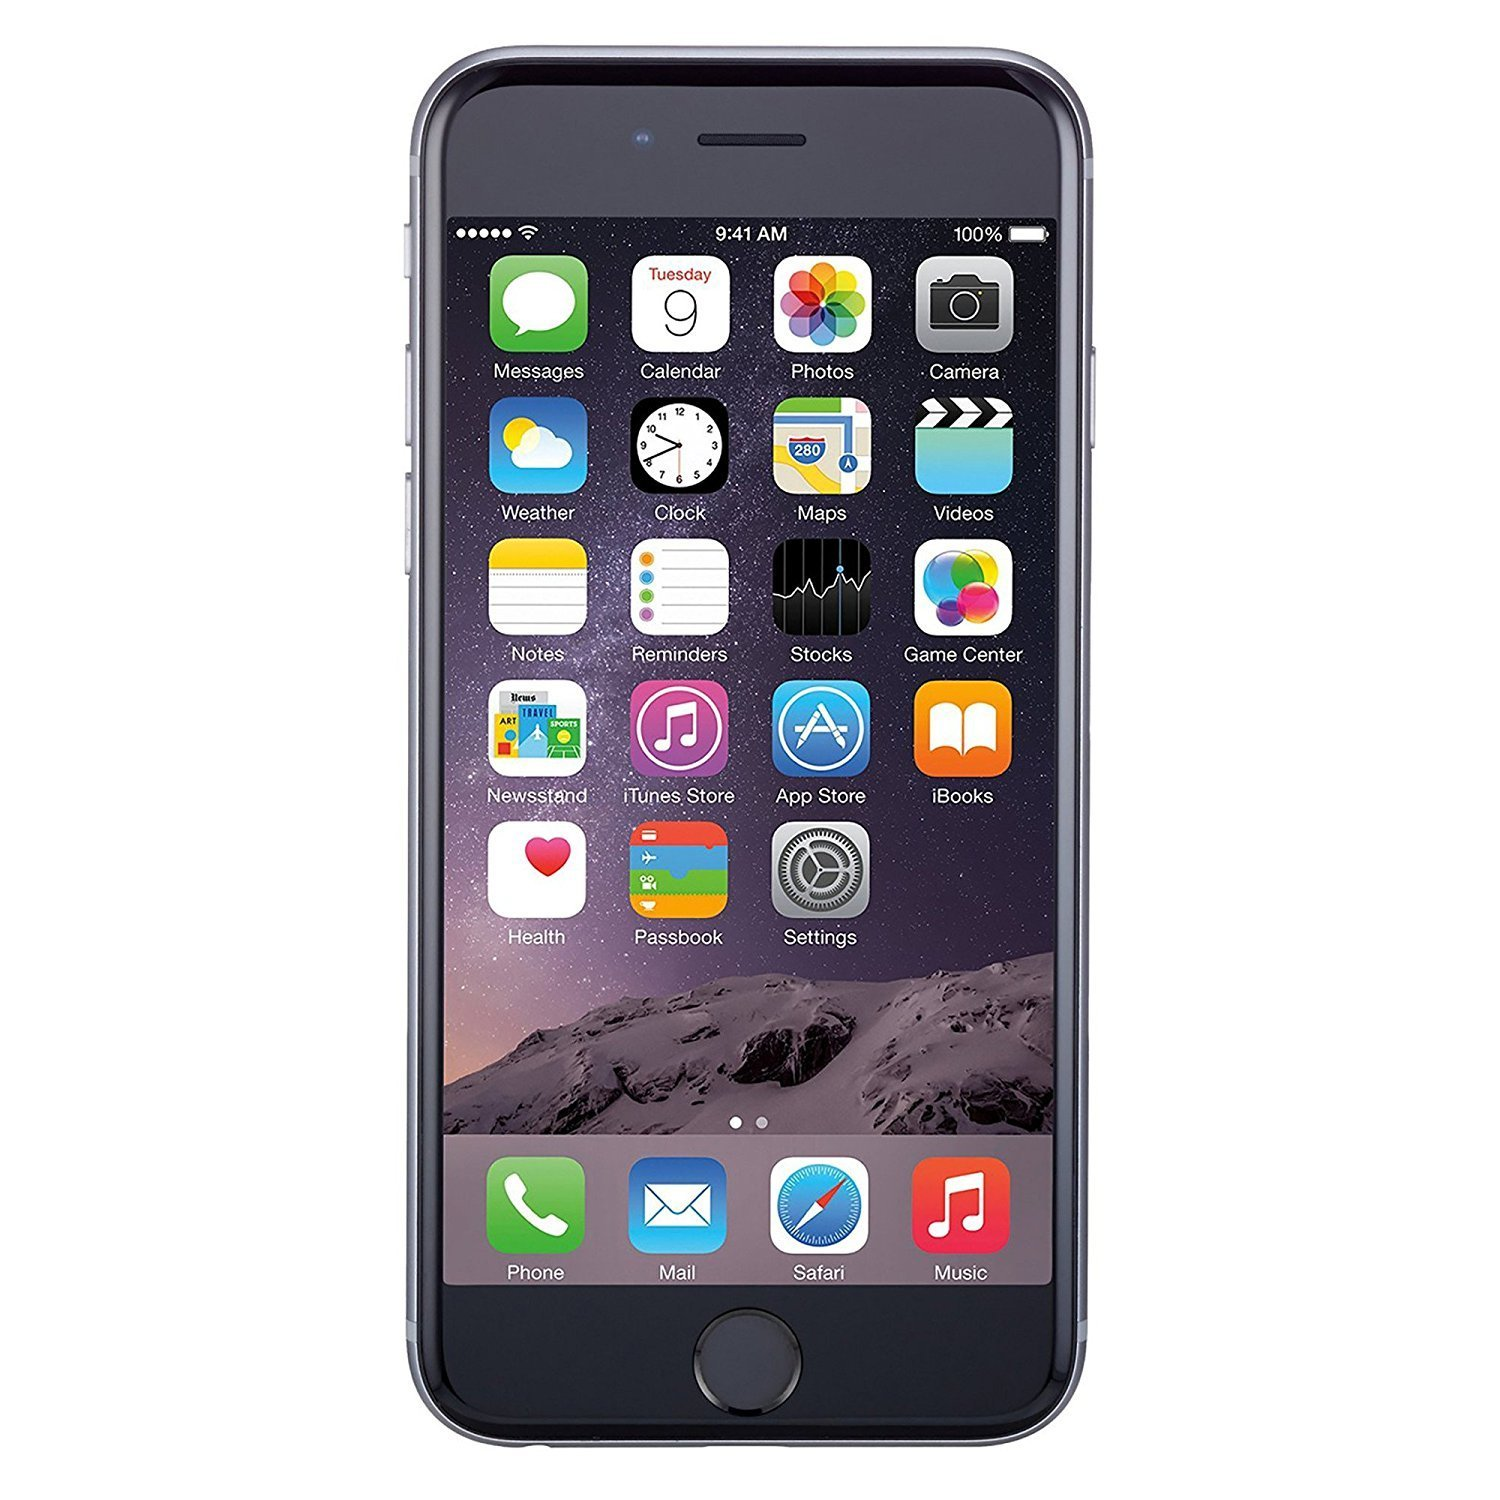
\includegraphics[width=\textwidth,height=1.5in]{images/iphone.jpg} &

\includegraphics[width=\textwidth,height=1.5in]{images/apps.jpg} \\
\bottomrule()
\end{longtable}

So R is like a new mobile phone: while it has a certain amount of
features when you use it for the first time, it doesn't have everything.
R packages are like the apps you can download onto your phone from
Apple's App Store or Android's Google Play.

Let's continue this analogy by considering the Instagram app for editing
and sharing pictures. Say you have purchased a new phone and you would
like to share a recent photo you have taken on Instagram. You need to:

\begin{enumerate}
\def\labelenumi{\arabic{enumi}.}
\item
  \emph{Install the app}: Since your phone is new and does not include
  the Instagram app, you need to download the app from either the App
  Store or Google Play. You do this once and you're set. You might do
  this again in the future any time there is an update to the app.
\item
  \emph{Open the app}: After you've installed Instagram, you need to
  open the app.
\end{enumerate}

Once Instagram is open on your phone, you can then proceed to share your
photo with your friends and family. The process is very similar for
using an R package. You need to:

\begin{enumerate}
\def\labelenumi{\arabic{enumi}.}
\item
  \emph{Install the package}: This is like installing an app on your
  phone. Most packages are not installed by default when you install R
  and RStudio. Thus if you want to use a package for the first time, you
  need to install it first. Once you've installed a package, you likely
  won't install it again unless you want to update it to a newer
  version.
\item
  \emph{``Load'' the package}: ``Loading'' a package is like opening an
  app on your phone. Packages are not ``loaded'' by default when you
  start RStudio on your computer; you need to ``load'' each package you
  want to use every time you start RStudio.
\end{enumerate}

Let's now show you how to perform these two steps for the
\texttt{ggplot2} package for data visualization.

\hypertarget{sec-package-installation}{%
\subsection{Package installation}\label{sec-package-installation}}

\begin{quote}
\textbf{Note about RStudio Server/Cloud}: If your instructor has
provided you with a link and access to RStudio Server/Cloud, you
probably will not need to install packages, as they have likely been
pre-installed for you by your instructor. That being said, it is still a
good idea to know this process for later on when you are not using
RStudio Server/Cloud, but rather RStudio Desktop on your own computer.
\end{quote}

There are two ways to install an R package. For example, to install the
\texttt{ggplot2} package:

\begin{enumerate}
\def\labelenumi{\arabic{enumi}.}
\item
  \textbf{Easy way}: In the Files pane of RStudio:

  \begin{enumerate}
  \def\labelenumii{\alph{enumii})}
  \item
    Click on the ``Packages'' tab
  \item
    Click on ``Install''
  \item
    Type the name of the package under ``Packages (separate multiple
    with space or comma):'' In this case, type \texttt{ggplot2}
  \item
    Click ``Install''

    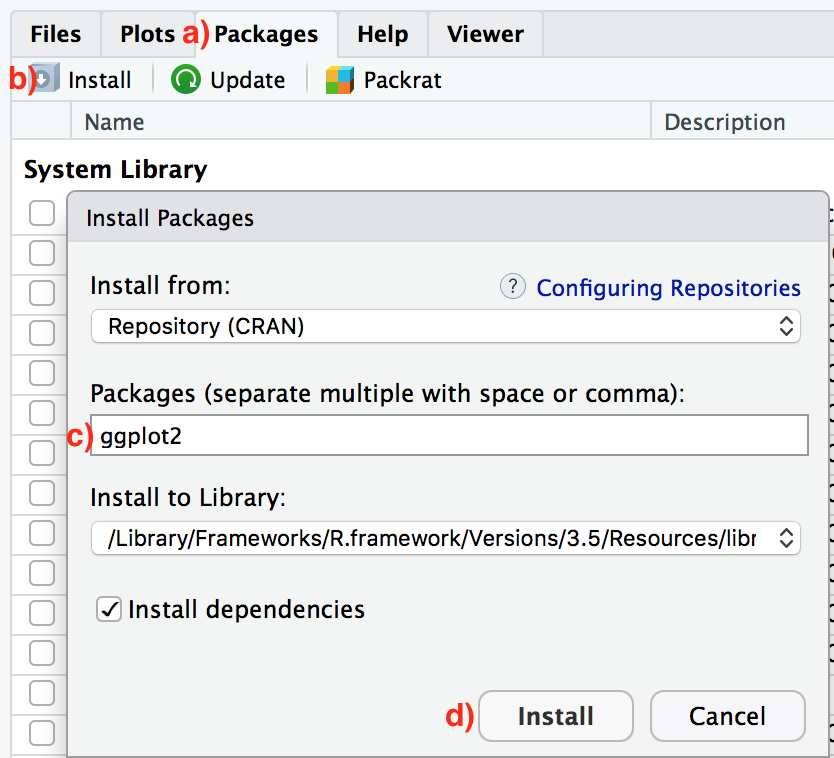
\includegraphics[width=\textwidth,height=4in]{images/install_packages_easy_way.png}
  \end{enumerate}
\item
  \textbf{Slightly harder way}: An alternative but slightly less
  convenient way to install a package is by typing
  \texttt{install.packages("ggplot2")} in the Console pane of RStudio
  and hitting enter. Note you must include the quotation marks.
\end{enumerate}

Much like an app on your phone, you only have to install a package once.
However, if you want to update an already installed package to a newer
verions, you need to re-install it by repeating the above steps.

\begin{tcolorbox}[enhanced jigsaw, coltitle=black, toprule=.15mm, bottomtitle=1mm, breakable, leftrule=.75mm, title={{🎯} Learning Check 1.1}, opacitybacktitle=0.6, colback=white, rightrule=.15mm, opacityback=0, toptitle=1mm, colbacktitle=quarto-callout-tip-color!10!white, colframe=quarto-callout-tip-color-frame, titlerule=0mm, arc=.35mm, bottomrule=.15mm, left=2mm]
Repeat the above installing steps for the \texttt{dplyr},
\texttt{nycflights13}, and \texttt{knitr} packages. This will install
the earlier mentioned \texttt{dplyr} package, the \texttt{nycflights13}
package containing data on all domestic flights leaving a NYC airport in
2013, and the \texttt{knitr} package for writing reports in R.
\end{tcolorbox}

\hypertarget{sec-package-loading}{%
\subsection{Package loading}\label{sec-package-loading}}

Recall that after you've installed a package, you need to ``load'' it,
in other words open it. We do this by using the \texttt{library()}
command. For example, to load the \texttt{ggplot2} package, run the
following code in the Console pane. What do we mean by ``run the
following code''? Either type or copy \& paste the following code into
the Console pane and then hit the enter key.

\begin{Shaded}
\begin{Highlighting}[]
\FunctionTok{library}\NormalTok{(ggplot2)}
\end{Highlighting}
\end{Shaded}

If after running the above code, a blinking cursor returns next to the
\texttt{\textgreater{}} ``prompt'' sign, it means you were successful
and the \texttt{ggplot2} package is now loaded and ready to use. If
however, you get a red ``error message'' that reads\ldots{}

\begin{verbatim}
Error in library(ggplot2) : there is no package called ‘ggplot2’
\end{verbatim}

\ldots{} it means that you didn't successfully install it. In that case,
go back to the previous subsection ``Package installation'' and install
it.

\begin{tcolorbox}[enhanced jigsaw, coltitle=black, toprule=.15mm, bottomtitle=1mm, breakable, leftrule=.75mm, title={{🎯} Learning Check 1.2}, opacitybacktitle=0.6, colback=white, rightrule=.15mm, opacityback=0, toptitle=1mm, colbacktitle=quarto-callout-tip-color!10!white, colframe=quarto-callout-tip-color-frame, titlerule=0mm, arc=.35mm, bottomrule=.15mm, left=2mm]
``Load'' the \texttt{dplyr}, \texttt{nycflights13}, and \texttt{knitr}
packages as well by repeating the above steps.
\end{tcolorbox}

\hypertarget{sec-package-use}{%
\subsection{Package use}\label{sec-package-use}}

One extremely common mistake new R users make when wanting to use
particular packages is that they forget to ``load'' them first by using
the \texttt{library()} command we just saw. Remember: \emph{you have to
load each package you want to use every time you start RStudio.} If you
don't first ``load'' a package, but attempt to use one of its features,
you'll see an error message similar to:

\begin{verbatim}
Error: could not find function
\end{verbatim}

R is telling you that you are trying to use a function in a package that
has not yet been ``loaded.'' Almost all new users forget do this when
starting out, and it is a little annoying to get used to. However,
you'll remember with practice.

\hypertarget{sec-nycflights13}{%
\section{Explore your first dataset}\label{sec-nycflights13}}

Let's put everything we've learned so far into practice and start
exploring some real data! Data comes to us in a variety of formats, from
pictures to text to numbers. Throughout this book, we'll focus on
datasets that are saved in ``spreadsheet''-type format; this is probably
the most common way data are collected and saved in many fields.
Remember from Subsection~\ref{sec-programming-concepts} that these
``spreadsheet''-type datasets are called \emph{data frames} in R; we
will focus on working with data saved as data frames throughout this
book.

Let's first load all the packages needed for this chapter, assuming
you've already installed them. Read Section~\ref{sec-packages} for
information on how to install and load R packages if you haven't
already.

\begin{Shaded}
\begin{Highlighting}[]
\FunctionTok{library}\NormalTok{(nycflights13)}
\FunctionTok{library}\NormalTok{(dplyr)}
\FunctionTok{library}\NormalTok{(knitr)}
\end{Highlighting}
\end{Shaded}

At the beginning of all subsequent chapters in this text, we'll always
have a list of packages that you should have installed and loaded to
work with that chapter's R code.

\hypertarget{nycflights13-package}{%
\subsection{\texorpdfstring{\texttt{nycflights13}
package}{nycflights13 package}}\label{nycflights13-package}}

Many of us have flown on airplanes or know someone who has. Air travel
has become an ever-present aspect in many people's lives. If you live in
or are visiting a relatively large city and you walk around that city's
airport, you see gates showing flight information from many different
airlines. And you will frequently see that some flights are delayed
because of a variety of conditions. Are there ways that we can avoid
having to deal with these flight delays?

We'd all like to arrive at our destinations on time whenever possible.
(Unless you secretly love hanging out at airports. If you are one of
these people, pretend for the moment that you are very much anticipating
being at your final destination.) Throughout this book, we're going to
analyze data related to flights contained in the \texttt{nycflights13}
package (Wickham 2021). Specifically, this package contains five data
sets saved in five separate data frames with information about all
domestic flights departing from New York City in 2013. These include
Newark Liberty International (EWR), John F. Kennedy International (JFK),
and LaGuardia (LGA) airports:

\begin{itemize}
\tightlist
\item
  \texttt{flights}: Information on all 336,776 flights
\item
  \texttt{airlines}: A table matching airline names and their two letter
  IATA airline codes (also known as carrier codes) for 16 airline
  companies
\item
  \texttt{planes}: Information about each of 3,322 physical aircraft
  used.
\item
  \texttt{weather}: Hourly meteorological data for each of the three NYC
  airports. This data frame has 26,115 rows, roughtly corresponding to
  the 365 \(\times\) 24 \(\times\) 3 = 26,280 possible hourly
  measurements one can observe at three locations over the course of a
  year.
\item
  \texttt{airports}: Airport names, codes, and locations for 1,458
  destination airports.
\end{itemize}

\hypertarget{flights-data-frame}{%
\subsection{\texorpdfstring{\texttt{flights} data
frame}{flights data frame}}\label{flights-data-frame}}

We will begin by exploring the \texttt{flights} data frame that is
included in the \texttt{nycflights13} package and getting an idea of its
structure. Run the following code in your console (either by typing it
or cutting \& pasting it): it loads in the \texttt{flights} dataset into
your Console. Note depending on the size of your monitor, the output may
vary slightly.

\begin{Shaded}
\begin{Highlighting}[]
\NormalTok{flights}
\end{Highlighting}
\end{Shaded}

\begin{verbatim}
# A tibble: 336,776 x 19
    year month   day dep_time sched_de~1 dep_d~2 arr_t~3 sched~4 arr_d~5 carrier
   <int> <int> <int>    <int>      <int>   <dbl>   <int>   <int>   <dbl> <chr>  
 1  2013     1     1      517        515       2     830     819      11 UA     
 2  2013     1     1      533        529       4     850     830      20 UA     
 3  2013     1     1      542        540       2     923     850      33 AA     
 4  2013     1     1      544        545      -1    1004    1022     -18 B6     
 5  2013     1     1      554        600      -6     812     837     -25 DL     
 6  2013     1     1      554        558      -4     740     728      12 UA     
 7  2013     1     1      555        600      -5     913     854      19 B6     
 8  2013     1     1      557        600      -3     709     723     -14 EV     
 9  2013     1     1      557        600      -3     838     846      -8 B6     
10  2013     1     1      558        600      -2     753     745       8 AA     
# ... with 336,766 more rows, 9 more variables: flight <int>, tailnum <chr>,
#   origin <chr>, dest <chr>, air_time <dbl>, distance <dbl>, hour <dbl>,
#   minute <dbl>, time_hour <dttm>, and abbreviated variable names
#   1: sched_dep_time, 2: dep_delay, 3: arr_time, 4: sched_arr_time,
#   5: arr_delay
\end{verbatim}

Let's unpack this output:

\begin{itemize}
\item
  \texttt{A\ tibble:\ 336,776\ x\ 19}: A \texttt{tibble} is a kind of
  data frame used in R. This particular data frame has

  \begin{itemize}
  \tightlist
  \item
    \texttt{336,776} rows
  \item
    \texttt{19} columns corresponding to 19 variables describing each
    observation
  \end{itemize}
\item
  \texttt{year\ month\ day\ dep\_time\ sched\_dep\_time\ dep\_delay\ arr\_time}
  are different columns, in other words variables, of this data frame.
\item
  We then have the first 10 rows of observations corresponding to 10
  flights.
\item
  \texttt{...\ with\ 336,766\ more\ rows,\ and\ 11\ more\ variables:}
  indicating to us that 336,766 more rows of data and 11 more variables
  could not fit in this screen.
\end{itemize}

Unfortunately, this output does not allow us to explore the data very
well. Let's look at different tools to explore data frames.

\hypertarget{sec-exploredataframes}{%
\subsection{Exploring data frames}\label{sec-exploredataframes}}

Among the many ways of getting a feel for the data contained in a data
frame such as \texttt{flights}, we present three functions that take as
their ``argument'', in other words their input, the data frame in
question. We also include a fourth method for exploring one particular
column of a data frame:

\begin{enumerate}
\def\labelenumi{\arabic{enumi}.}
\tightlist
\item
  Using the \texttt{View()} function built for use in RStudio. We will
  use this the most.
\item
  Using the \texttt{glimpse()} function, which is included in the
  \texttt{dplyr} package.
\item
  Using the \texttt{kable()} function, which is included in the
  \texttt{knitr} package.
\item
  Using the \texttt{\$} operator to view a single variable in a data
  frame.
\end{enumerate}

\textbf{1. \texttt{View()}}:

Run \texttt{View(flights)} in your Console in RStudio, either by typing
it or cutting \& pasting it into the Console pane, and explore this data
frame in the resulting pop-up viewer. You should get into the habit of
always \texttt{View}ing any data frames that come your way. Note the
capital ``V'' in \texttt{View}. R is case-sensitive so you'll receive an
error is you run \texttt{view(flights)} instead of
\texttt{View(flights)}.

\begin{tcolorbox}[enhanced jigsaw, coltitle=black, toprule=.15mm, bottomtitle=1mm, breakable, leftrule=.75mm, title={{🎯} Learning Check 1.3}, opacitybacktitle=0.6, colback=white, rightrule=.15mm, opacityback=0, toptitle=1mm, colbacktitle=quarto-callout-tip-color!10!white, colframe=quarto-callout-tip-color-frame, titlerule=0mm, arc=.35mm, bottomrule=.15mm, left=2mm]

What does any \emph{ONE} row in this \texttt{flights} dataset refer to?

\begin{enumerate}
\def\labelenumi{\alph{enumi}.}
\tightlist
\item
  Data on an airline
\item
  Data on a flight
\item
  Data on an airport
\item
  Data on multiple flights
\end{enumerate}

\end{tcolorbox}

By running \texttt{View(flights)}, we see the different \emph{variables}
listed in the columns and we see that there are different types of
variables. Some of the variables like \texttt{distance}, \texttt{day},
and \texttt{arr\_delay} are what we will call \emph{quantitative}
variables. These variables are numerical in nature. Other variables here
are \emph{categorical}.

Note that if you look in the leftmost column of the
\texttt{View(flights)} output, you will see a column of numbers. These
are the row numbers of the dataset. If you glance across a row with the
same number, say row 5, you can get an idea of what each row corresponds
to. In other words, this will allow you to identify what object is being
referred to in a given row. This is often called the \emph{observational
unit}. The \emph{observational unit} in this example is an individual
flight departing New York City in 2013. You can identify the
observational unit by determining what ``thing'' is being measured or
described by each of the variables.

\textbf{2. \texttt{glimpse()}}:

The second way to explore a data frame is using the \texttt{glimpse()}
function included in the \texttt{dplyr} package. Thus, you can only use
the \texttt{glimpse()} function after you've loaded the \texttt{dplyr}
package. This function provides us with an alternative method for
exploring a data frame:

\begin{Shaded}
\begin{Highlighting}[]
\FunctionTok{glimpse}\NormalTok{(flights)}
\end{Highlighting}
\end{Shaded}

\begin{verbatim}
Rows: 336,776
Columns: 19
$ year           <int> 2013, 2013, 2013, 2013, 2013, 2013, 2013, 2013, 2013, 2~
$ month          <int> 1, 1, 1, 1, 1, 1, 1, 1, 1, 1, 1, 1, 1, 1, 1, 1, 1, 1, 1~
$ day            <int> 1, 1, 1, 1, 1, 1, 1, 1, 1, 1, 1, 1, 1, 1, 1, 1, 1, 1, 1~
$ dep_time       <int> 517, 533, 542, 544, 554, 554, 555, 557, 557, 558, 558, ~
$ sched_dep_time <int> 515, 529, 540, 545, 600, 558, 600, 600, 600, 600, 600, ~
$ dep_delay      <dbl> 2, 4, 2, -1, -6, -4, -5, -3, -3, -2, -2, -2, -2, -2, -1~
$ arr_time       <int> 830, 850, 923, 1004, 812, 740, 913, 709, 838, 753, 849,~
$ sched_arr_time <int> 819, 830, 850, 1022, 837, 728, 854, 723, 846, 745, 851,~
$ arr_delay      <dbl> 11, 20, 33, -18, -25, 12, 19, -14, -8, 8, -2, -3, 7, -1~
$ carrier        <chr> "UA", "UA", "AA", "B6", "DL", "UA", "B6", "EV", "B6", "~
$ flight         <int> 1545, 1714, 1141, 725, 461, 1696, 507, 5708, 79, 301, 4~
$ tailnum        <chr> "N14228", "N24211", "N619AA", "N804JB", "N668DN", "N394~
$ origin         <chr> "EWR", "LGA", "JFK", "JFK", "LGA", "EWR", "EWR", "LGA",~
$ dest           <chr> "IAH", "IAH", "MIA", "BQN", "ATL", "ORD", "FLL", "IAD",~
$ air_time       <dbl> 227, 227, 160, 183, 116, 150, 158, 53, 140, 138, 149, 1~
$ distance       <dbl> 1400, 1416, 1089, 1576, 762, 719, 1065, 229, 944, 733, ~
$ hour           <dbl> 5, 5, 5, 5, 6, 5, 6, 6, 6, 6, 6, 6, 6, 6, 6, 5, 6, 6, 6~
$ minute         <dbl> 15, 29, 40, 45, 0, 58, 0, 0, 0, 0, 0, 0, 0, 0, 0, 59, 0~
$ time_hour      <dttm> 2013-01-01 05:00:00, 2013-01-01 05:00:00, 2013-01-01 0~
\end{verbatim}

We see that \texttt{glimpse()} will give you the first few entries of
each variable in a row after the variable. In addition, the \emph{data
type} (see Subsection~\ref{sec-programming-concepts}) of the variable is
given immediately after each variable's name inside
\texttt{\textless{}\ \textgreater{}}. Here, \texttt{int} and
\texttt{dbl} refer to ``integer'' and ``double'', which are computer
coding terminology for quantitative/numerical variables. In contrast,
\texttt{chr} refers to ``character'', which is computer terminology for
text data. Text data, such as the \texttt{carrier} or \texttt{origin} of
a flight, are categorical variables. The \texttt{time\_hour} variable is
an example of one more type of data type: \texttt{dttm}. As you may
suspect, this variable corresponds to a specific date and time of day.
However, we won't work with dates in this class and leave it to a more
advanced book on data science.

\begin{tcolorbox}[enhanced jigsaw, coltitle=black, toprule=.15mm, bottomtitle=1mm, breakable, leftrule=.75mm, title={{🎯} Learning Check 1.4}, opacitybacktitle=0.6, colback=white, rightrule=.15mm, opacityback=0, toptitle=1mm, colbacktitle=quarto-callout-tip-color!10!white, colframe=quarto-callout-tip-color-frame, titlerule=0mm, arc=.35mm, bottomrule=.15mm, left=2mm]
What are some examples in this dataset of \textbf{categorical}
variables? What makes them different than \textbf{quantitative}
variables?
\end{tcolorbox}

\textbf{3. \texttt{kable()}}:

The another way to explore the entirety of a data frame is using the
\texttt{kable()} function from the \texttt{knitr} package. Let's explore
the different carrier codes for all the airlines in our dataset two
ways. Run both of these lines of code in your Console:

\begin{Shaded}
\begin{Highlighting}[]
\NormalTok{airlines}
\FunctionTok{kable}\NormalTok{(airlines)}
\end{Highlighting}
\end{Shaded}

At first glance, it may not appear that there is much difference in the
outputs. However when using tools for document production such as
\href{https://quarto.org/docs/get-started/hello/rstudio.html}{Quarto},
the latter code produces output that is much more legible and
reader-friendly.

\textbf{4. \texttt{\$} operator}

Lastly, the \texttt{\$} operator allows us to explore a single variable
within a data frame. For example, run the following in your console

\begin{Shaded}
\begin{Highlighting}[]
\NormalTok{airlines}
\NormalTok{airlines}\SpecialCharTok{$}\NormalTok{name}
\end{Highlighting}
\end{Shaded}

We used the \texttt{\$} operator to extract only the \texttt{name}
variable and return it as a vector of length 16. We will only be
occasionally exploring data frames using this operator, instead favoring
the \texttt{View()} and \texttt{glimpse()} functions.

\hypertarget{help-files}{%
\subsection{Help files}\label{help-files}}

Another nice feature of R is the help system. You can get help in R by
entering a \texttt{?} before the name of a function or data frame in
question and you will be presented with a page showing the
documentation. For example, let's look at the help file for the
\texttt{flights} data frame:

\begin{Shaded}
\begin{Highlighting}[]
\NormalTok{?flights}
\end{Highlighting}
\end{Shaded}

A help file should pop-up in the Help pane of RStudio. If you have
questions about a function or data frame included in an R package, you
should get in the habit of consulting the help file right away.

\hypertarget{sec-gs-conclusion}{%
\section{Conclusion}\label{sec-gs-conclusion}}

We've given you what we feel are the most essential concepts to know
before you can start exploring data in R. Is this chapter exhaustive?
Absolutely not. To try to include everything in this chapter would make
the chapter so large it wouldn't be useful!

\hypertarget{additional-resources}{%
\subsection{Additional resources}\label{additional-resources}}

If you are completely new to the world of coding, R, and RStudio and
feel you could benefit from a more detailed introduction, we suggest you
check out Chester Ismay's short book
\href{https://rbasics.netlify.com/}{Getting used to R, RStudio, and R
Markdown} (Ismay 2016), which includes screencast recordings that you
can follow along and pause as you learn. While this book teaches R
Markdown it it important to note that everything in R Markdown is
transferable to Quarto. R Markdown and Quarto are both tools used for
reproducible research but R Markdown is fundamentally tied to R while
Quarto is a multi-language platform. For a getting started guide on
Quarto, we suggest the
\href{https://quarto.org/docs/get-started/hello/rstudio.html}{Quarto
Getting Started webpage}

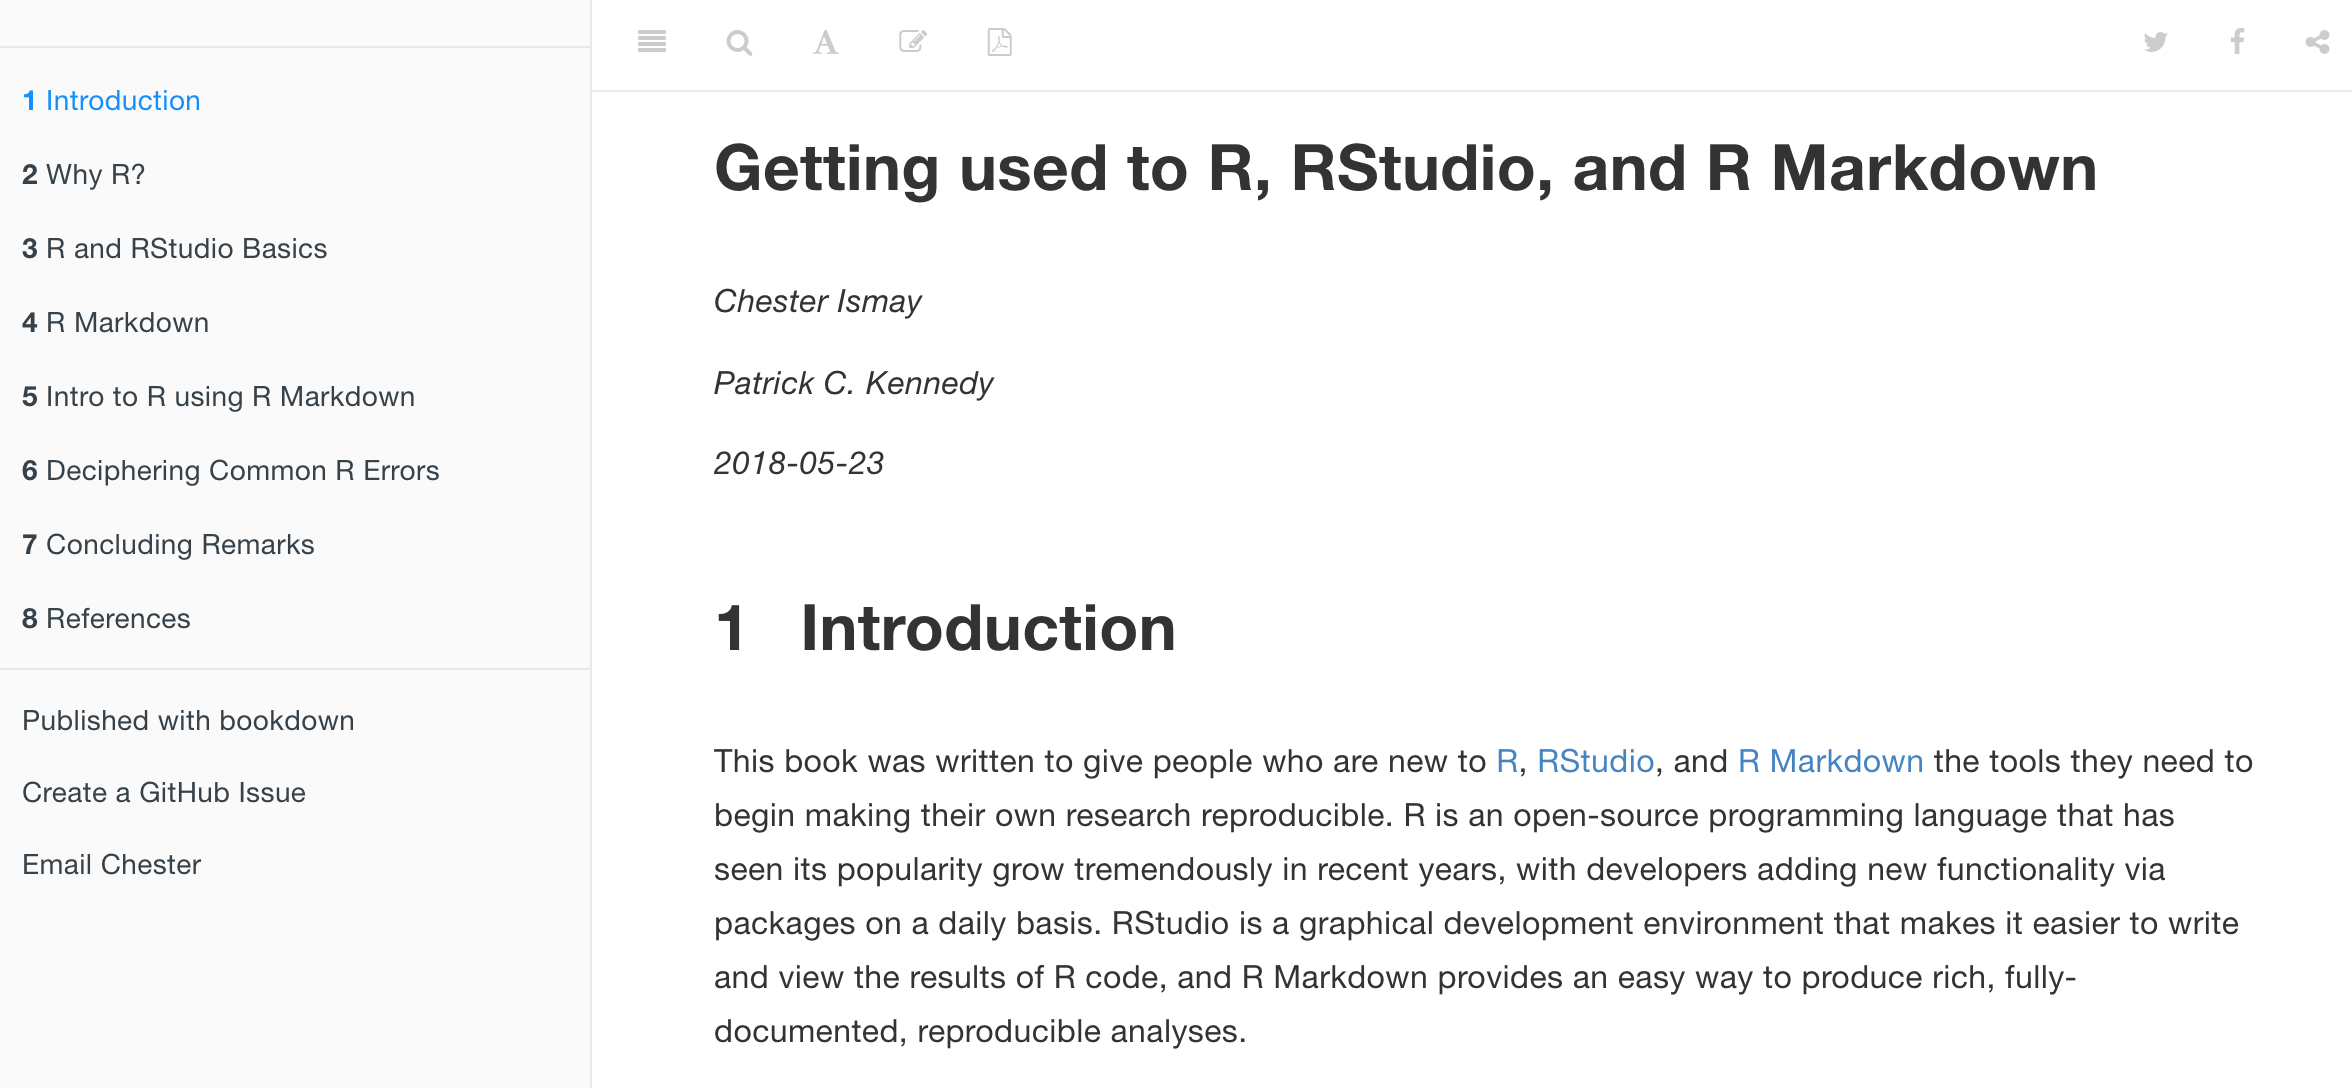
\includegraphics[width=\textwidth,height=3.5in]{images/gettting-used-to-R.png}

\hypertarget{sec-ex01}{%
\section{Exercises}\label{sec-ex01}}

\hypertarget{sec-ex00-explained}{%
\subsection{Exercises explained}\label{sec-ex00-explained}}

Following each chapter, there are a set of Exercises for you to practice
what you have learned. The \textbf{Conceptual} questions are multiple
choice or short answer questions focusing on the major concepts learned
throughout the chapter. The \textbf{Application} questions focus on
practical skills learned throughout the chapter. And the
\textbf{Advanced} questions teach new and useful skills beyond what was
taught in the chapter.

The chapter exercises use the \texttt{covid\_states}, \texttt{nba}, and
\texttt{titanic} datasets which are included in the
\texttt{ISDSdatasets} package. To install \texttt{ISDSdatasets} on your
computer, type \texttt{remotes::install\_github("NUstat/ISDSdatasets")}
in your \textbf{Console}. You may need to install the \texttt{remotes}
package first. See Section~\ref{sec-package-installation} for how to
install the \texttt{remotes} package. If you are using RStudio Cloud,
your instructor probably already installed all of this for you. You can
see what packages you have installed by clicking on the
\textbf{Packages} tab in the lower right pane.

To use the package make sure you load it using
\texttt{library(ISDSdatasets)}. To explore a dataset within the package
you can use the \texttt{View()} or \texttt{data()} function in your
\textbf{Console}. For example, try typing \texttt{data(titanic)} in the
\textbf{Console}. This will load the \texttt{titanic} data into the
\textbf{Environment}.

\hypertarget{sec-ex01-conceptual}{%
\subsection{Conceptual}\label{sec-ex01-conceptual}}

\leavevmode\vadjust pre{\hypertarget{exr-ch01-c01}{}}%
\begin{exercise}[]\label{exr-ch01-c01}

Which type of document do we use to both code and write explanations?

\begin{enumerate}
\def\labelenumi{\alph{enumi})}
\tightlist
\item
  R Script
\item
  Quarto Document
\item
  HTML file
\item
  R Notebook
\end{enumerate}

\end{exercise}

\leavevmode\vadjust pre{\hypertarget{exr-ch01-c02}{}}%
\begin{exercise}[]\label{exr-ch01-c02}

Which type of red text in the console pane generally means that your
code will not run?

\begin{enumerate}
\def\labelenumi{\alph{enumi})}
\tightlist
\item
  error
\item
  warning
\item
  message
\end{enumerate}

\end{exercise}

\leavevmode\vadjust pre{\hypertarget{exr-ch01-c03}{}}%
\begin{exercise}[]\label{exr-ch01-c03}

If you place the operator ? before the name of a function or data frame,
then you will be presented with a page showing the documentation for the
respective function or data frame.

\begin{enumerate}
\def\labelenumi{\alph{enumi})}
\tightlist
\item
  TRUE
\item
  FALSE
\end{enumerate}

\end{exercise}

\leavevmode\vadjust pre{\hypertarget{exr-ch01-c04}{}}%
\begin{exercise}[]\label{exr-ch01-c04}

If you type \texttt{8/2\ ==\ 4} into the console, what will the output
be?

\begin{enumerate}
\def\labelenumi{\alph{enumi})}
\tightlist
\item
  TRUE
\item
  FALSE
\item
  NA
\item
  0
\item
  4
\end{enumerate}

\end{exercise}

\leavevmode\vadjust pre{\hypertarget{exr-ch01-c05}{}}%
\begin{exercise}[]\label{exr-ch01-c05}

If you type \texttt{3\^{}2\ !=\ 9} into the console, what will the
output be?

\begin{enumerate}
\def\labelenumi{\alph{enumi})}
\tightlist
\item
  TRUE
\item
  FALSE
\item
  NA
\item
  0
\item
  9
\end{enumerate}

\end{exercise}

\leavevmode\vadjust pre{\hypertarget{exr-ch01-c06}{}}%
\begin{exercise}[]\label{exr-ch01-c06}

If you type \texttt{5*3} into the console, what will the output be?

\begin{enumerate}
\def\labelenumi{\alph{enumi})}
\tightlist
\item
  TRUE
\item
  FALSE
\item
  NA
\item
  8
\item
  15
\end{enumerate}

\end{exercise}

\leavevmode\vadjust pre{\hypertarget{exr-ch01-c07}{}}%
\begin{exercise}[]\label{exr-ch01-c07}

What does any ONE row in this flights dataset refer to?

\begin{enumerate}
\def\labelenumi{\alph{enumi})}
\tightlist
\item
  Data on an airline
\item
  Data on a flight
\item
  Data on an airport
\item
  Data on multiple flights
\end{enumerate}

\end{exercise}

\leavevmode\vadjust pre{\hypertarget{exr-ch01-c08}{}}%
\begin{exercise}[]\label{exr-ch01-c08}

In the flights dataset, \texttt{air\_time} and \texttt{arr\_delay} are
which type of variables?

\begin{enumerate}
\def\labelenumi{\alph{enumi})}
\tightlist
\item
  string
\item
  categorical
\item
  quantitative
\item
  character
\item
  dataframe
\end{enumerate}

\end{exercise}

\hypertarget{sec-ex01-application}{%
\subsection{Application}\label{sec-ex01-application}}

\leavevmode\vadjust pre{\hypertarget{exr-ch01-app1}{}}%
\begin{exercise}[]\label{exr-ch01-app1}

In a code chunk, first define a variable \texttt{z} to be the product of
12 and 31, then define a variable called \texttt{add\_on} to be the
number 12. Print the output of \texttt{z\ +\ add\_on}.

\end{exercise}

\leavevmode\vadjust pre{\hypertarget{exr-ch01-app2}{}}%
\begin{exercise}[]\label{exr-ch01-app2}

Consider the \texttt{titanic} data set included in the package
\texttt{ISDSdatasets}. This is one of the most popular data sets used
for understanding machine learning basics, and you will likely see this
data set in the future if you continue on in your studies to machine
learning.

Use the \texttt{glimpse()} function from the \texttt{dplyr} package to
explore and describe the dataset.

\end{exercise}

\hypertarget{sec-ex01-advanced}{%
\subsection{Advanced}\label{sec-ex01-advanced}}

For the following problems we will use the \texttt{titanic} data set to
learn additional data exploration techniques.

\leavevmode\vadjust pre{\hypertarget{exr-ch01-adv1}{}}%
\begin{exercise}[]\label{exr-ch01-adv1}

Use the function \texttt{head()} on the \texttt{titanic} dataset. What
does it do? Based on this, what do you expect the function
\texttt{tail()} does?

\end{exercise}

\leavevmode\vadjust pre{\hypertarget{exr-ch01-adv2}{}}%
\begin{exercise}[]\label{exr-ch01-adv2}

The function \texttt{unique()}, when used on a specific variable within
a data set, returns a vector of the values of the variable with
duplicate elements removed. Try using the function \texttt{unique()} on
the variable \texttt{Embarked}.

\end{exercise}

\part{Data Exploration via the tidyverse}

\hypertarget{sec-viz}{%
\chapter{Data Visualization}\label{sec-viz}}

We begin the development of your data science toolbox with data
visualization. By visualizing our data, we gain valuable insights that
we couldn't initially see from just looking at the raw data in
spreadsheet form. We will use the \texttt{ggplot2} package as it
provides an easy way to customize your plots. \texttt{ggplot2} is rooted
in the data visualization theory known as \emph{The Grammar of Graphics}
(Wilkinson 2005).

At the most basic level, graphics/plots/charts (we use these terms
interchangeably in this book) provide a nice way for us to get a sense
for how quantitative variables compare in terms of their center (where
the values tend to be located) and their spread (how they vary around
the center). Graphics should be designed to emphasize the findings and
insight you want your audience to understand. This does however require
a balancing act. On the one hand, you want to highlight as many
meaningful relationships and interesting findings as possible; on the
other you don't want to include so many as to overwhelm your audience.

As we will see, plots/graphics also help us to identify patterns and
outliers in our data. We will see that a common extension of these ideas
is to compare the \emph{distribution} of one quantitative variable
(i.e., what the spread of a variable looks like or how the variable is
\emph{distributed} in terms of its values) as we go across the levels of
a different categorical variable.

\hypertarget{packages-needed}{%
\section*{Packages Needed}\label{packages-needed}}
\addcontentsline{toc}{section}{Packages Needed}

Let's load all the packages needed for this chapter (this assumes you've
already installed them). Read Section~\ref{sec-packages} for information
on how to install and load R packages.

\begin{Shaded}
\begin{Highlighting}[]
\FunctionTok{library}\NormalTok{(nycflights13)}
\FunctionTok{library}\NormalTok{(ggplot2)}
\FunctionTok{library}\NormalTok{(dplyr)}
\end{Highlighting}
\end{Shaded}

\hypertarget{sec-grammarofgraphics}{%
\section{The Grammar of Graphics}\label{sec-grammarofgraphics}}

We begin with a discussion of a theoretical framework for data
visualization known as ``The Grammar of Graphics,'' which serves as the
foundation for the \texttt{ggplot2} package. Think of how we construct
sentences in English to form sentences by combining different elements,
like nouns, verbs, particles, subjects, objects, etc. However, we can't
just combine these elements in any arbitrary order; we must do so
following a set of rules known as a linguistic grammar. Similarly to a
linguistic grammar, ``The Grammar of Graphics'' define a set of rules
for constructing \emph{statistical graphics} by combining different
types of \emph{layers}. This grammar was created by Leland Wilkinson
(Wilkinson 2005) and has been implemented in a variety of data
visualization software including R.

\hypertarget{components-of-the-grammar}{%
\subsection{Components of the Grammar}\label{components-of-the-grammar}}

In short, the grammar tells us that:

\begin{quote}
\textbf{A statistical graphic is a \texttt{mapping} of \texttt{data}
variables to \texttt{aes}thetic attributes of \texttt{geom}etric
objects.}
\end{quote}

Specifically, we can break a graphic into three essential components:

\begin{enumerate}
\def\labelenumi{\arabic{enumi}.}
\tightlist
\item
  \texttt{data}: the data set composed of variables that we map.
\item
  \texttt{geom}: the geometric object in question. This refers to the
  type of object we can observe in a plot. For example: points, lines,
  and bars.
\item
  \texttt{aes}: aesthetic attributes of the geometric object. For
  example, x-position, y-position, color, shape, and size. Each assigned
  aesthetic attribute can be mapped to a variable in our data set.
\end{enumerate}

You might be wondering why we wrote the terms \texttt{data},
\texttt{geom}, and \texttt{aes} in a computer code type font. We'll see
very shortly that we'll specify the elements of the grammar in R using
these terms. However, let's first break down the grammar with an
example.

\hypertarget{sec-gapminder}{%
\subsection{Gapminder data}\label{sec-gapminder}}

In February 2006, a statistician named Hans Rosling gave a TED talk
titled
\href{https://www.ted.com/talks/hans_rosling_shows_the_best_stats_you_ve_ever_seen}{``The
best stats you've ever seen''} where he presented global economic,
health, and development data from the website
\href{http://www.gapminder.org/tools/\#_locale_id=en;\&chart-type=bubbles}{gapminder.org}.
For example, for the 142 countries included from 2007, let's consider
only the first 6 countries when listed alphabetically in
Table~\ref{tbl-gapminder-2007}.

\hypertarget{tbl-gapminder-2007}{}
\begin{longtable}[]{@{}llrrr@{}}
\caption{\label{tbl-gapminder-2007}Gapminder 2007 Data: First 6 of 142
countries}\tabularnewline
\toprule()
Country & Continent & Life Expectancy & Population & GDP per Capita \\
\midrule()
\endfirsthead
\toprule()
Country & Continent & Life Expectancy & Population & GDP per Capita \\
\midrule()
\endhead
Afghanistan & Asia & 43.8 & 31889923 & 975 \\
Albania & Europe & 76.4 & 3600523 & 5937 \\
Algeria & Africa & 72.3 & 33333216 & 6223 \\
Angola & Africa & 42.7 & 12420476 & 4797 \\
Argentina & Americas & 75.3 & 40301927 & 12779 \\
Australia & Oceania & 81.2 & 20434176 & 34435 \\
\bottomrule()
\end{longtable}

Each row in this table corresponds to a country in 2007. For each row,
we have 5 columns:

\begin{enumerate}
\def\labelenumi{\arabic{enumi}.}
\tightlist
\item
  \textbf{Country}: Name of country.
\item
  \textbf{Continent}: Which of the five continents the country is part
  of. (Note that ``Americas'' includes countries in both North and South
  America and that Antarctica is excluded.)
\item
  \textbf{Life Expectancy}: Life expectancy in years.
\item
  \textbf{Population}: Number of people living in the country.
\item
  \textbf{GDP per Capita}: Gross domestic product (in US dollars).
\end{enumerate}

Now consider Figure~\ref{fig-gapminder}, which plots this data for all
142 countries in the data.

\begin{figure}

{\centering 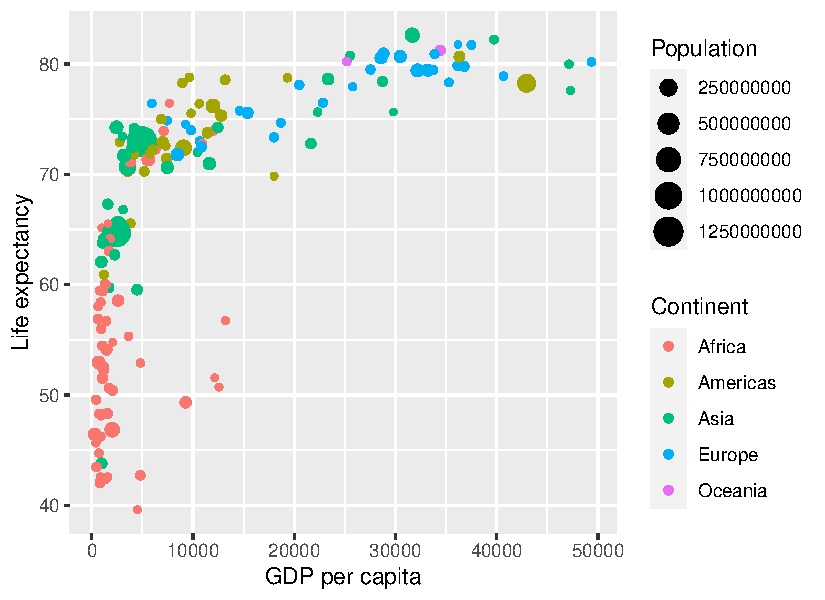
\includegraphics{02-visualization_files/figure-pdf/fig-gapminder-1.pdf}

}

\caption{\label{fig-gapminder}Life Expectancy over GDP per Capita in
2007}

\end{figure}

Let's view this plot through the grammar of graphics:

\begin{enumerate}
\def\labelenumi{\arabic{enumi}.}
\tightlist
\item
  The \texttt{data} variable \textbf{GDP per Capita} gets mapped to the
  \texttt{x}-position \texttt{aes}thetic of the points.
\item
  The \texttt{data} variable \textbf{Life Expectancy} gets mapped to the
  \texttt{y}-position \texttt{aes}thetic of the points.
\item
  The \texttt{data} variable \textbf{Population} gets mapped to the
  \texttt{size} \texttt{aes}thetic of the points.
\item
  The \texttt{data} variable \textbf{Continent} gets mapped to the
  \texttt{color} \texttt{aes}thetic of the points.
\end{enumerate}

We'll see shortly that \texttt{data} corresponds to the particular data
frame where our data is saved and a ``data variable'' corresponds to a
particular column in the data frame. Furthermore, the type of
\texttt{geom}etric object considered in this plot are points. That being
said, while in this example we are considering points, graphics are not
limited to just points. Other plots involve lines while others involve
bars.

Let's summarize the three essential components of the Grammar in
Table~\ref{tbl-summary-gapminder}.

\hypertarget{tbl-summary-gapminder}{}
\begin{longtable}[]{@{}lll@{}}
\caption{\label{tbl-summary-gapminder}Summary of Grammar of Graphics for
this plot}\tabularnewline
\toprule()
data variable & aes & geom \\
\midrule()
\endfirsthead
\toprule()
data variable & aes & geom \\
\midrule()
\endhead
GDP per Capita & x & point \\
Life Expectancy & y & point \\
Population & size & point \\
Continent & color & point \\
\bottomrule()
\end{longtable}

\hypertarget{other-components}{%
\subsection{Other components}\label{other-components}}

There are other components of the Grammar of Graphics we can control as
well. As you start to delve deeper into the Grammar of Graphics, you'll
start to encounter these topics more frequently. In this book however,
we'll keep things simple and only work with the two additional
components listed below:

\begin{itemize}
\tightlist
\item
  \texttt{facet}ing breaks up a plot into small multiples corresponding
  to the levels of another variable (Section~\ref{sec-facets})
\item
  \texttt{position} adjustments for barplots (Section~\ref{sec-geombar})
\end{itemize}

Other more complex components like \texttt{scales} and
\texttt{coord}inate systems are left for a more advanced text such as
\href{http://r4ds.had.co.nz/data-visualisation.html\#aesthetic-mappings}{R
for Data Science} (Grolemund and Wickham 2016). Generally speaking, the
Grammar of Graphics allows for a high degree of customization of plots
and also a consistent framework for easily updating and modifying them.

\hypertarget{ggplot2-package}{%
\subsection{ggplot2 package}\label{ggplot2-package}}

In this book, we will be using the \texttt{ggplot2} package for data
visualization, which is an implementation of the Grammar of Graphics for
R (Wickham et al. 2022). As we noted earlier, a lot of the previous
section was written in a computer code type font. This is because the
various components of the Grammar of Graphics are specified in the
\texttt{ggplot()} function included in the \texttt{ggplot2} package,
which expects at a minimum as arguments (i.e.~inputs):

\begin{itemize}
\tightlist
\item
  The data frame where the variables exist: the \texttt{data} argument.
\item
  The mapping of the variables to aesthetic attributes: the
  \texttt{mapping} argument which specifies the \texttt{aes}thetic
  attributes involved.
\end{itemize}

After we've specified these components, we then add \emph{layers} to the
plot using the \texttt{+} sign. The most essential layer to add to a
plot is the layer that specifies which type of \texttt{geom}etric object
we want the plot to involve: points, lines, bars, and others. Other
layers we can add to a plot include layers specifying the plot title,
axes labels, visual themes for the plots, and facets (which we'll see in
Section~\ref{sec-facets}.

Let's now put the theory of the Grammar of Graphics into practice.

\hypertarget{sec-five-ng}{%
\section{Five Named Graphs - The 5NG}\label{sec-five-ng}}

In order to keep things simple, we will only focus on five types of
graphics in this book, each with a commonly given name. We term these
``five named graphs'' the \textbf{5NG}:

\begin{enumerate}
\def\labelenumi{\arabic{enumi}.}
\tightlist
\item
  scatterplots
\item
  linegraphs
\item
  boxplots
\item
  histograms
\item
  barplots
\end{enumerate}

We will discuss some variations of these plots, but with this basic
repertoire of graphics in your toolbox you can visualize a wide array of
different variable types. Note that certain plots are only appropriate
for categorical variables and while others are only appropriate for
quantitative variables. You'll want to quiz yourself often as we go
along on which plot makes sense a given a particular problem or data
set.

\hypertarget{sec-scatterplots}{%
\section{5NG\#1: Scatterplots}\label{sec-scatterplots}}

The simplest of the 5NG are \emph{scatterplots}, also called bivariate
plots. They allow you to visualize the relationship between two
numerical variables. While you may already be familiar with
scatterplots, let's view them through the lens of the Grammar of
Graphics. Specifically, we will visualize the relationship between the
following two numerical variables in the \texttt{flights} data frame
included in the \texttt{nycflights13} package:

\begin{enumerate}
\def\labelenumi{\arabic{enumi}.}
\tightlist
\item
  \texttt{dep\_delay}: departure delay on the horizontal ``x'' axis and
\item
  \texttt{arr\_delay}: arrival delay on the vertical ``y'' axis
\end{enumerate}

for Alaska Airlines flights leaving NYC in 2013. This requires paring
down the data from all 336,776 flights that left NYC in 2013, to only
the 714 \emph{Alaska Airlines} flights that left NYC in 2013.

What this means computationally is: we'll take the \texttt{flights} data
frame, extract only the 714 rows corresponding to Alaska Airlines
flights, and save this in a new data frame called
\texttt{alaska\_flights}. Run the code below to do this:

\begin{Shaded}
\begin{Highlighting}[]
\NormalTok{alaska\_flights }\OtherTok{\textless{}{-}}\NormalTok{ flights }\SpecialCharTok{\%\textgreater{}\%} 
  \FunctionTok{filter}\NormalTok{(carrier }\SpecialCharTok{==} \StringTok{"AS"}\NormalTok{)}
\end{Highlighting}
\end{Shaded}

For now we suggest you ignore how this code works; we'll explain this in
detail in Chapter~\ref{sec-wrangling} when we cover data wrangling.
However, convince yourself that this code does what it is supposed to by
running \texttt{View(alaska\_flights)}: it creates a new data frame
\texttt{alaska\_flights} consisting of only the 714 Alaska Airlines
flights.

We'll see later in Chapter~\ref{sec-wrangling} on data wrangling that
this code uses the \texttt{dplyr} package for data wrangling to achieve
our goal: it takes the \texttt{flights} data frame and \texttt{filter}s
it to only return the rows where \texttt{carrier} is equal to
\texttt{"AS"}, Alaska Airlines' carrier code. Other examples of carrier
codes include ``AA'' for American Airlines and ``UA'' for United
Airlines. Recall from Section~\ref{sec-code} that testing for equality
is specified with \texttt{==} and not \texttt{=}. Fasten your seat belts
and sit tight for now however, we'll introduce these ideas more fully in
Chapter~\ref{sec-wrangling}.

\begin{tcolorbox}[enhanced jigsaw, coltitle=black, toprule=.15mm, bottomtitle=1mm, breakable, leftrule=.75mm, title={{🎯} Learning Check 2.1}, opacitybacktitle=0.6, colback=white, rightrule=.15mm, opacityback=0, toptitle=1mm, colbacktitle=quarto-callout-tip-color!10!white, colframe=quarto-callout-tip-color-frame, titlerule=0mm, arc=.35mm, bottomrule=.15mm, left=2mm]
Take a look at both the \texttt{flights} and \texttt{alaska\_flights}
data frames by running \texttt{View(flights)} and
\texttt{View(alaska\_flights)}. In what respect do these data frames
differ?
\end{tcolorbox}

\hypertarget{sec-geompoint}{%
\subsection{Scatterplots via geom\_point}\label{sec-geompoint}}

Let's now go over the code that will create the desired scatterplot,
keeping in mind our discussion on the Grammar of Graphics in
Section~\ref{sec-grammarofgraphics}. We'll be using the
\texttt{ggplot()} function included in the \texttt{ggplot2} package.

\begin{Shaded}
\begin{Highlighting}[]
\FunctionTok{ggplot}\NormalTok{(}\AttributeTok{data =}\NormalTok{ alaska\_flights, }\AttributeTok{mapping =} \FunctionTok{aes}\NormalTok{(}\AttributeTok{x =}\NormalTok{ dep\_delay, }\AttributeTok{y =}\NormalTok{ arr\_delay)) }\SpecialCharTok{+} 
  \FunctionTok{geom\_point}\NormalTok{()}
\end{Highlighting}
\end{Shaded}

Let's break this down piece-by-piece:

\begin{itemize}
\tightlist
\item
  Within the \texttt{ggplot()} function, we specify two of the
  components of the Grammar of Graphics as arguments (i.e.~inputs):

  \begin{enumerate}
  \def\labelenumi{\arabic{enumi}.}
  \tightlist
  \item
    The \texttt{data} frame to be \texttt{alaska\_flights} by setting
    \texttt{data\ =\ alaska\_flights}.
  \item
    The \texttt{aes}thetic \texttt{mapping} by setting
    \texttt{aes(x\ =\ dep\_delay,\ y\ =\ arr\_delay)}. Specifically:

    \begin{itemize}
    \tightlist
    \item
      the variable \texttt{dep\_delay} maps to the \texttt{x} position
      aesthetic
    \item
      the variable \texttt{arr\_delay} maps to the \texttt{y} position
      aesthetic
    \end{itemize}
  \end{enumerate}
\item
  We add a layer to the \texttt{ggplot()} function call using the
  \texttt{+} sign. The layer in question specifies the third component
  of the grammar: the \texttt{geom}etric object. In this case the
  geometric object are points, set by specifying \texttt{geom\_point()}.
\end{itemize}

After running the above code, you'll notice two outputs: a warning
message and the graphic shown in Figure~\ref{fig-noalpha}. Let's first
unpack the warning message:

\begin{verbatim}
Warning: Removed 5 rows containing missing values (geom_point).
\end{verbatim}

\begin{figure}

{\centering 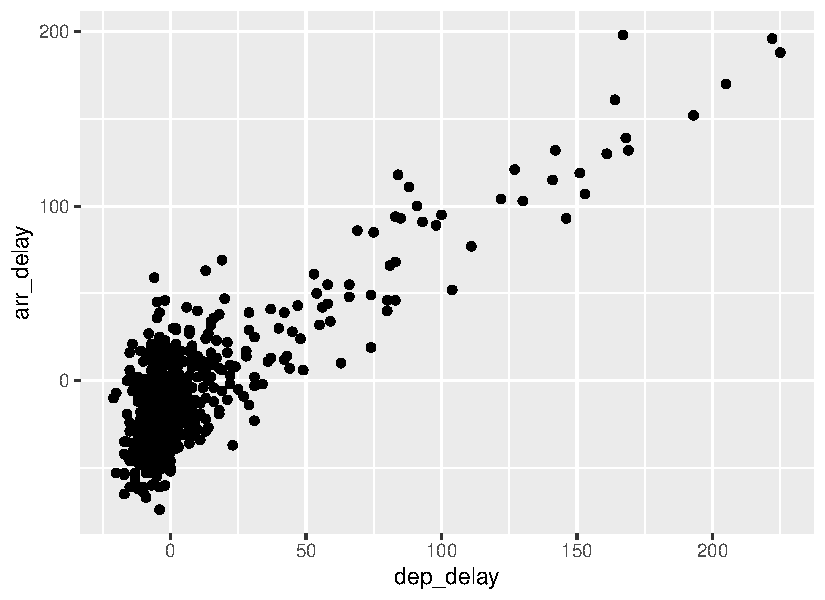
\includegraphics{02-visualization_files/figure-pdf/fig-noalpha-1.pdf}

}

\caption{\label{fig-noalpha}Arrival Delays vs Departure Delays for
Alaska Airlines flights from NYC in 2013}

\end{figure}

After running the above code, R returns a warning message alerting us to
the fact that 5 rows were ignored due to them being missing. For 5 rows
either the value for \texttt{dep\_delay} or \texttt{arr\_delay} or both
were missing (recorded in R as \texttt{NA}), and thus these rows were
ignored in our plot. Turning our attention to the resulting scatterplot
in Figure~\ref{fig-noalpha}, we see that a positive relationship exists
between \texttt{dep\_delay} and \texttt{arr\_delay}: as departure delays
increase, arrival delays tend to also increase. We also note the large
mass of points clustered near (0, 0).

Before we continue, let's consider a few more notes on the layers in the
above code that generated the scatterplot:

\begin{itemize}
\tightlist
\item
  Note that the \texttt{+} sign comes at the end of lines, and not at
  the beginning. You'll get an error in R if you put it at the
  beginning.
\item
  When adding layers to a plot, you are encouraged to start a new line
  after the \texttt{+} so that the code for each layer is on a new line.
  As we add more and more layers to plots, you'll see this will greatly
  improve the legibility of your code.
\item
  To stress the importance of adding layers in particular the layer
  specifying the \texttt{geom}etric object, consider
  Figure~\ref{fig-nolayers} where no layers are added. A not very useful
  plot!
\end{itemize}

\begin{Shaded}
\begin{Highlighting}[]
\FunctionTok{ggplot}\NormalTok{(}\AttributeTok{data =}\NormalTok{ alaska\_flights, }\AttributeTok{mapping =} \FunctionTok{aes}\NormalTok{(}\AttributeTok{x =}\NormalTok{ dep\_delay, }\AttributeTok{y =}\NormalTok{ arr\_delay))}
\end{Highlighting}
\end{Shaded}

\begin{figure}[H]

{\centering 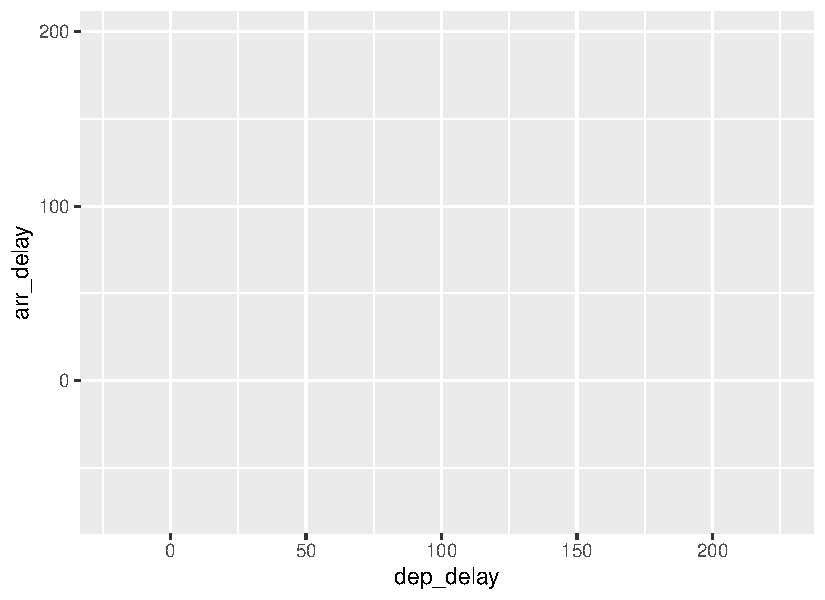
\includegraphics{02-visualization_files/figure-pdf/fig-nolayers-1.pdf}

}

\caption{\label{fig-nolayers}Plot with no layers}

\end{figure}

\begin{tcolorbox}[enhanced jigsaw, coltitle=black, toprule=.15mm, bottomtitle=1mm, breakable, leftrule=.75mm, title={{🎯} Learning Check 2.2}, opacitybacktitle=0.6, colback=white, rightrule=.15mm, opacityback=0, toptitle=1mm, colbacktitle=quarto-callout-tip-color!10!white, colframe=quarto-callout-tip-color-frame, titlerule=0mm, arc=.35mm, bottomrule=.15mm, left=2mm]
What are some practical reasons why \texttt{dep\_delay} and
\texttt{arr\_delay} have a positive relationship?
\end{tcolorbox}

\begin{tcolorbox}[enhanced jigsaw, coltitle=black, toprule=.15mm, bottomtitle=1mm, breakable, leftrule=.75mm, title={{🎯} Learning Check 2.3}, opacitybacktitle=0.6, colback=white, rightrule=.15mm, opacityback=0, toptitle=1mm, colbacktitle=quarto-callout-tip-color!10!white, colframe=quarto-callout-tip-color-frame, titlerule=0mm, arc=.35mm, bottomrule=.15mm, left=2mm]
What variables (not necessarily in the \texttt{flights} data frame)
would you expect to have a negative correlation (i.e.~a negative
relationship) with \texttt{dep\_delay}? Why? Remember that we are
focusing on numerical variables here.
\end{tcolorbox}

\begin{tcolorbox}[enhanced jigsaw, coltitle=black, toprule=.15mm, bottomtitle=1mm, breakable, leftrule=.75mm, title={{🎯} Learning Check 2.4}, opacitybacktitle=0.6, colback=white, rightrule=.15mm, opacityback=0, toptitle=1mm, colbacktitle=quarto-callout-tip-color!10!white, colframe=quarto-callout-tip-color-frame, titlerule=0mm, arc=.35mm, bottomrule=.15mm, left=2mm]
Why do you believe there is a cluster of points near (0, 0)? What does
(0, 0) correspond to in terms of the Alaskan flights?
\end{tcolorbox}

\begin{tcolorbox}[enhanced jigsaw, coltitle=black, toprule=.15mm, bottomtitle=1mm, breakable, leftrule=.75mm, title={{🎯} Learning Check 2.5}, opacitybacktitle=0.6, colback=white, rightrule=.15mm, opacityback=0, toptitle=1mm, colbacktitle=quarto-callout-tip-color!10!white, colframe=quarto-callout-tip-color-frame, titlerule=0mm, arc=.35mm, bottomrule=.15mm, left=2mm]
What are some other features of the plot that stand out to you?
\end{tcolorbox}

\begin{tcolorbox}[enhanced jigsaw, coltitle=black, toprule=.15mm, bottomtitle=1mm, breakable, leftrule=.75mm, title={{🎯} Learning Check 2.6}, opacitybacktitle=0.6, colback=white, rightrule=.15mm, opacityback=0, toptitle=1mm, colbacktitle=quarto-callout-tip-color!10!white, colframe=quarto-callout-tip-color-frame, titlerule=0mm, arc=.35mm, bottomrule=.15mm, left=2mm]
Create a new scatterplot using different variables in the
\texttt{alaska\_flights} data frame by modifying the example above.
\end{tcolorbox}

\hypertarget{sec-overplotting}{%
\subsection{Over-plotting}\label{sec-overplotting}}

The large mass of points near (0, 0) in Figure~\ref{fig-noalpha} can
cause some confusion as it is hard to tell the true number of points
that are plotted. This is the result of a phenomenon called
\emph{overplotting}. As one may guess, this corresponds to values being
plotted on top of each other \emph{over} and \emph{over} again. It is
often difficult to know just how many values are plotted in this way
when looking at a basic scatterplot as we have here. There are two
methods to address the issue of overplotting:

\begin{enumerate}
\def\labelenumi{\arabic{enumi}.}
\tightlist
\item
  By adjusting the transparency of the points.
\item
  By adding a little random ``jitter'', or random ``nudges'', to each of
  the points.
\end{enumerate}

\textbf{Method 1: Changing the transparency}

The first way of addressing overplotting is by changing the transparency
of the points by using the \texttt{alpha} argument in
\texttt{geom\_point()}. By default, this value is set to \texttt{1}. We
can change this to any value between \texttt{0} and \texttt{1}, where
\texttt{0} sets the points to be 100\% transparent and \texttt{1} sets
the points to be 100\% opaque. Note how the following code is identical
to the code in Section~\ref{sec-scatterplots} that created the
scatterplot with overplotting, but with \texttt{alpha\ =\ 0.2} added to
the \texttt{geom\_point()}:

\begin{Shaded}
\begin{Highlighting}[]
\FunctionTok{ggplot}\NormalTok{(}\AttributeTok{data =}\NormalTok{ alaska\_flights, }\AttributeTok{mapping =} \FunctionTok{aes}\NormalTok{(}\AttributeTok{x =}\NormalTok{ dep\_delay, }\AttributeTok{y =}\NormalTok{ arr\_delay)) }\SpecialCharTok{+} 
  \FunctionTok{geom\_point}\NormalTok{(}\AttributeTok{alpha =} \FloatTok{0.2}\NormalTok{)}
\end{Highlighting}
\end{Shaded}

\begin{figure}[H]

{\centering 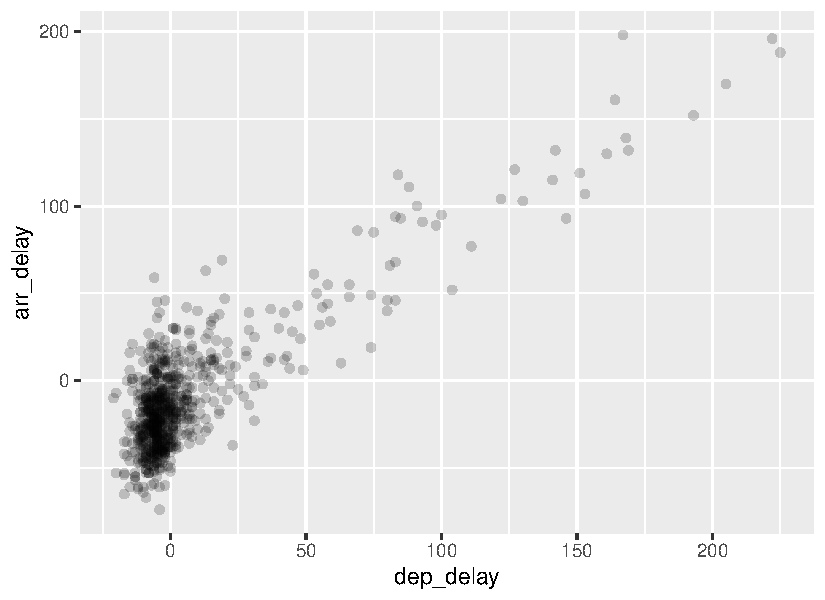
\includegraphics{02-visualization_files/figure-pdf/fig-alpha-1.pdf}

}

\caption{\label{fig-alpha}Delay scatterplot with alpha = 0.2}

\end{figure}

The key feature to note in Figure~\ref{fig-alpha} is that the
transparency of the points is cumulative: areas with a high-degree of
overplotting are darker, whereas areas with a lower degree are less
dark. Note furthermore that there is no \texttt{aes()} surrounding
\texttt{alpha\ =\ 0.2}. This is because we are not mapping a variable to
an aesthetic attribute, but rather merely changing the default setting
of \texttt{alpha}. In fact, you'll receive an error if you try to change
the second line above to read \texttt{geom\_point(aes(alpha\ =\ 0.2))}.

\textbf{Method 2: Jittering the points}

The second way of addressing overplotting is by \emph{jittering} all the
points, in other words give each point a small nudge in a random
direction. You can think of ``jittering'' as shaking the points around a
bit on the plot. Let's illustrate using a simple example first. Say we
have a data frame \texttt{jitter\_example} with 4 rows of identical
value 0 for both \texttt{x} and \texttt{y}:

\begin{verbatim}
# A tibble: 4 x 2
      x     y
  <dbl> <dbl>
1     0     0
2     0     0
3     0     0
4     0     0
\end{verbatim}

We display the resulting scatterplot in
Figure~\ref{fig-jitter-example-plot-1}; observe that the 4 points are
superimposed on top of each other. While we know there are 4 values
being plotted, this fact might not be apparent to others.

\begin{figure}

{\centering 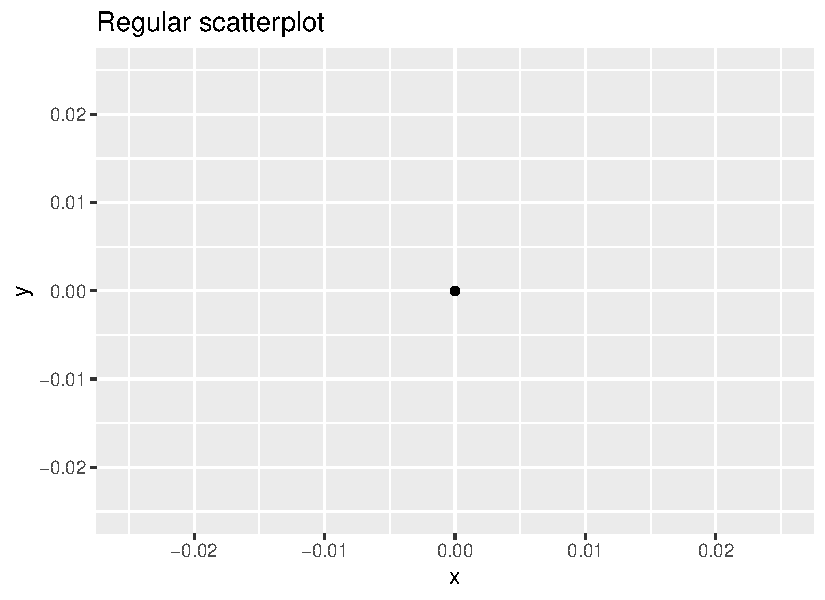
\includegraphics{02-visualization_files/figure-pdf/fig-jitter-example-plot-1-1.pdf}

}

\caption{\label{fig-jitter-example-plot-1}Regular scatterplot of jitter
example data}

\end{figure}

In Figure~\ref{fig-jitter-example-plot-2} we instead display a
\emph{jittered scatterplot} where each point is given a random
``nudge.'' It is now plainly evident that this plot involves four
points. Keep in mind that jittering is strictly a visualization tool;
even after creating a jittered scatterplot, the original values saved in
\texttt{jitter\_example} remain unchanged.

\begin{figure}

{\centering 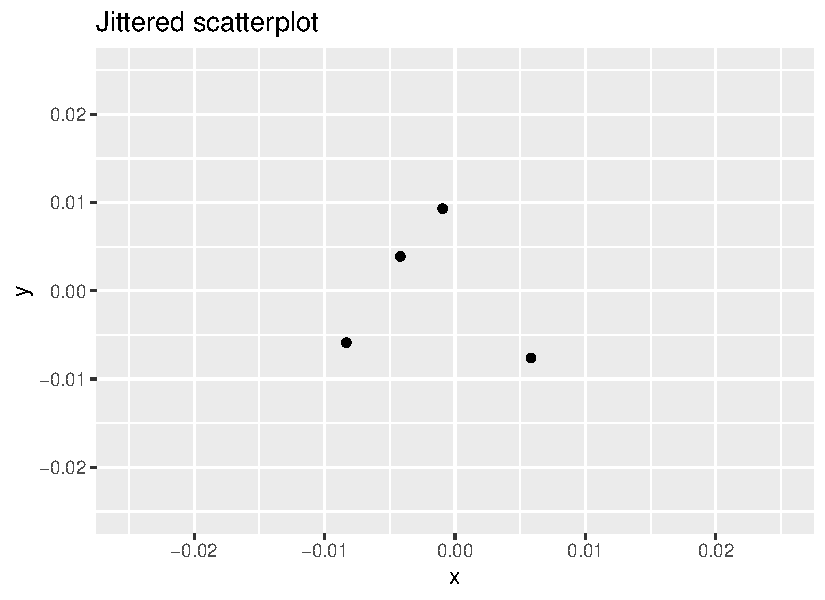
\includegraphics{02-visualization_files/figure-pdf/fig-jitter-example-plot-2-1.pdf}

}

\caption{\label{fig-jitter-example-plot-2}Jittered scatterplot of jitter
example data}

\end{figure}

To create a jittered scatterplot, instead of using
\texttt{geom\_point()}, we use \texttt{geom\_jitter()}. To specify how
much jitter to add, we adjust the \texttt{width} and \texttt{height}
arguments. This corresponds to how hard you'd like to shake the plot in
units corresponding to those for both the horizontal and vertical
variables (in this case minutes).

\begin{Shaded}
\begin{Highlighting}[]
\FunctionTok{ggplot}\NormalTok{(}\AttributeTok{data =}\NormalTok{ alaska\_flights, }\AttributeTok{mapping =} \FunctionTok{aes}\NormalTok{(}\AttributeTok{x =}\NormalTok{ dep\_delay, }\AttributeTok{y =}\NormalTok{ arr\_delay)) }\SpecialCharTok{+} 
  \FunctionTok{geom\_jitter}\NormalTok{(}\AttributeTok{width =} \DecValTok{30}\NormalTok{, }\AttributeTok{height =} \DecValTok{30}\NormalTok{)}
\end{Highlighting}
\end{Shaded}

\begin{figure}[H]

{\centering 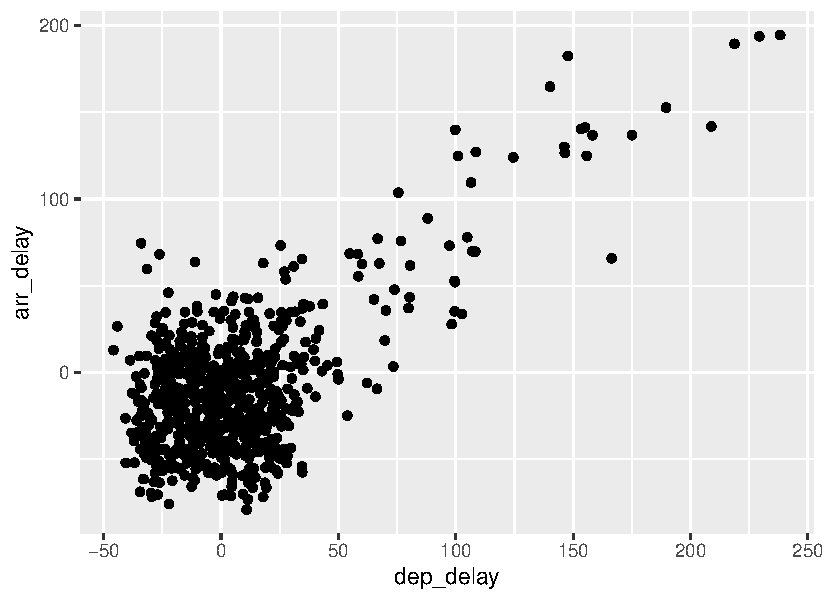
\includegraphics{02-visualization_files/figure-pdf/fig-jitter-1.pdf}

}

\caption{\label{fig-jitter}Jittered delay scatterplot}

\end{figure}

Observe how the above code is identical to the code that created the
scatterplot with overplotting in Subsection~\ref{sec-geompoint}, but
with \texttt{geom\_point()} replaced with \texttt{geom\_jitter()}.

The resulting plot in Figure~\ref{fig-jitter} helps us a little bit in
getting a sense for the overplotting, but with a relatively large data
set like this one (714 flights), it can be argued that changing the
transparency of the points by setting \texttt{alpha} proved more
effective. In terms of how much jitter one should add using the
\texttt{width} and \texttt{height} arguments, it is important to add
just enough jitter to break any overlap in points, but not so much that
we completely alter the overall pattern in points.

\begin{tcolorbox}[enhanced jigsaw, coltitle=black, toprule=.15mm, bottomtitle=1mm, breakable, leftrule=.75mm, title={{🎯} Learning Check 2.7}, opacitybacktitle=0.6, colback=white, rightrule=.15mm, opacityback=0, toptitle=1mm, colbacktitle=quarto-callout-tip-color!10!white, colframe=quarto-callout-tip-color-frame, titlerule=0mm, arc=.35mm, bottomrule=.15mm, left=2mm]
Why is setting the \texttt{alpha} argument value useful with
scatterplots? What further information does it give you that a regular
scatterplot cannot?
\end{tcolorbox}

\begin{tcolorbox}[enhanced jigsaw, coltitle=black, toprule=.15mm, bottomtitle=1mm, breakable, leftrule=.75mm, title={{🎯} Learning Check 2.8}, opacitybacktitle=0.6, colback=white, rightrule=.15mm, opacityback=0, toptitle=1mm, colbacktitle=quarto-callout-tip-color!10!white, colframe=quarto-callout-tip-color-frame, titlerule=0mm, arc=.35mm, bottomrule=.15mm, left=2mm]
After viewing the Figure~\ref{fig-alpha} above, give an approximate
range of arrival delays and departure delays that occur the most
frequently. How has that region changed compared to when you observed
the same plot without the \texttt{alpha\ =\ 0.2} set in
Figure~\ref{fig-noalpha}?
\end{tcolorbox}

\hypertarget{summary}{%
\subsection{Summary}\label{summary}}

Scatterplots display the relationship between two numerical variables.
They are among the most commonly used plots because they can provide an
immediate way to see the trend in one variable versus another. However,
if you try to create a scatterplot where either one of the two variables
is not numerical, you might get strange results. Be careful!

With medium to large data sets, you may need to play around with the
different modifications one can make to a scatterplot. This tweaking is
often a fun part of data visualization, since you'll have the chance to
see different relationships come about as you make subtle changes to
your plots.

\hypertarget{sec-linegraphs}{%
\section{5NG\#2: Linegraphs}\label{sec-linegraphs}}

The next of the five named graphs are linegraphs. Linegraphs show the
relationship between two numerical variables when the variable on the
x-axis, also called the \emph{explanatory} variable, is of a sequential
nature; in other words there is an inherent ordering to the variable.
The most common example of linegraphs have some notion of time on the
x-axis: hours, days, weeks, years, etc. Since time is sequential, we
connect consecutive observations of the variable on the y-axis with a
line. Linegraphs that have some notion of time on the x-axis are also
called \emph{time series} plots. Linegraphs should be avoided when there
is not a clear sequential ordering to the variable on the x-axis. Let's
illustrate linegraphs using another data set in the
\texttt{nycflights13} package: the \texttt{weather} data frame.

Let's get a sense for the \texttt{weather} data frame:

\begin{itemize}
\tightlist
\item
  Explore the \texttt{weather} data by running \texttt{View(weather)}.
\item
  Run \texttt{?weather} to bring up the help file.
\end{itemize}

We can see that there is a variable called \texttt{temp} of hourly
temperature recordings in Fahrenheit at weather stations near all three
airports in New York City: Newark (\texttt{origin} code \texttt{EWR}),
JFK, and La Guardia (\texttt{LGA}). Instead of considering hourly
temperatures for all days in 2013 for all three airports however, for
simplicity let's only consider hourly temperatures at only Newark
airport for the first 15 days in January.

Recall in Section~\ref{sec-scatterplots} we used the \texttt{filter()}
function to only choose the subset of rows of \texttt{flights}
corresponding to Alaska Airlines flights. We similarly use
\texttt{filter()} here, but by using the \texttt{\&} operator we only
choose the subset of rows of \texttt{weather} where

\begin{enumerate}
\def\labelenumi{\arabic{enumi}.}
\tightlist
\item
  The \texttt{origin} is \texttt{"EWR"} and
\item
  the \texttt{month} is January and
\item
  the \texttt{day} is between \texttt{1} and \texttt{15}
\end{enumerate}

\begin{Shaded}
\begin{Highlighting}[]
\NormalTok{early\_january\_weather }\OtherTok{\textless{}{-}}\NormalTok{ weather }\SpecialCharTok{\%\textgreater{}\%} 
  \FunctionTok{filter}\NormalTok{(origin }\SpecialCharTok{==} \StringTok{"EWR"} \SpecialCharTok{\&}\NormalTok{ month }\SpecialCharTok{==} \DecValTok{1} \SpecialCharTok{\&}\NormalTok{ day }\SpecialCharTok{\textless{}=} \DecValTok{15}\NormalTok{)}
\end{Highlighting}
\end{Shaded}

\begin{tcolorbox}[enhanced jigsaw, coltitle=black, toprule=.15mm, bottomtitle=1mm, breakable, leftrule=.75mm, title={{🎯} Learning Check 2.9}, opacitybacktitle=0.6, colback=white, rightrule=.15mm, opacityback=0, toptitle=1mm, colbacktitle=quarto-callout-tip-color!10!white, colframe=quarto-callout-tip-color-frame, titlerule=0mm, arc=.35mm, bottomrule=.15mm, left=2mm]
Take a look at both the \texttt{weather} and
\texttt{early\_january\_weather} data frames by running
\texttt{View(weather)} and \texttt{View(early\_january\_weather)}. In
what respect do these data frames differ?
\end{tcolorbox}

\begin{tcolorbox}[enhanced jigsaw, coltitle=black, toprule=.15mm, bottomtitle=1mm, breakable, leftrule=.75mm, title={{🎯} Learning Check 2.10}, opacitybacktitle=0.6, colback=white, rightrule=.15mm, opacityback=0, toptitle=1mm, colbacktitle=quarto-callout-tip-color!10!white, colframe=quarto-callout-tip-color-frame, titlerule=0mm, arc=.35mm, bottomrule=.15mm, left=2mm]
\texttt{View()} the \texttt{flights} data frame again. Why does the
\texttt{time\_hour} variable uniquely identify the hour of the
measurement whereas the \texttt{hour} variable does not?
\end{tcolorbox}

\hypertarget{sec-geomline}{%
\subsection{Linegraphs via geom\_line}\label{sec-geomline}}

Let's plot a linegraph of hourly temperatures in
\texttt{early\_january\_weather} by using \texttt{geom\_line()} instead
of \texttt{geom\_point()} like we did for scatterplots:

\begin{Shaded}
\begin{Highlighting}[]
\FunctionTok{ggplot}\NormalTok{(}\AttributeTok{data =}\NormalTok{ early\_january\_weather, }\AttributeTok{mapping =} \FunctionTok{aes}\NormalTok{(}\AttributeTok{x =}\NormalTok{ time\_hour, }\AttributeTok{y =}\NormalTok{ temp)) }\SpecialCharTok{+}
  \FunctionTok{geom\_line}\NormalTok{()}
\end{Highlighting}
\end{Shaded}

\begin{figure}[H]

{\centering 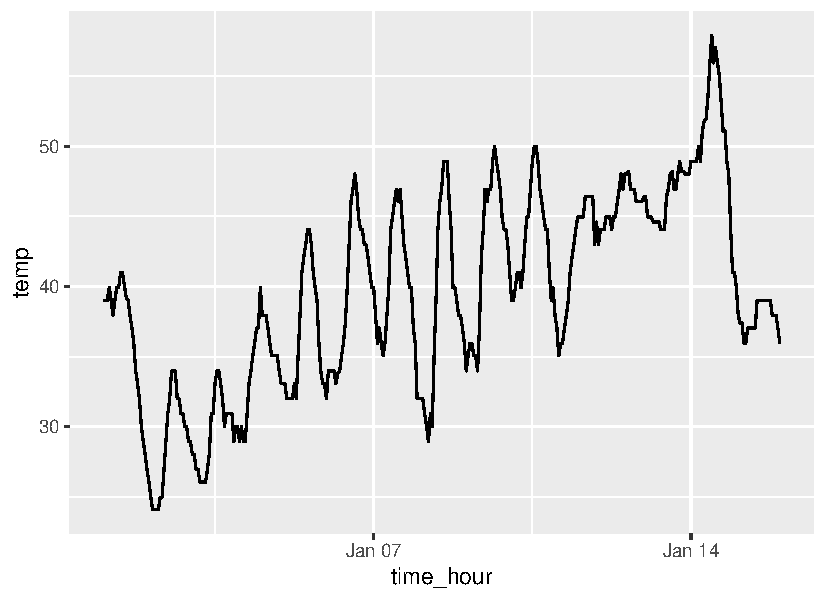
\includegraphics{02-visualization_files/figure-pdf/fig-hourlytemp-1.pdf}

}

\caption{\label{fig-hourlytemp}Hourly Temperature in Newark for January
1-15, 2013}

\end{figure}

Much as with the \texttt{ggplot()} code that created the scatterplot of
departure and arrival delays for Alaska Airlines flights in
Figure~\ref{fig-noalpha}, let's break down the above code piece-by-piece
in terms of the Grammar of Graphics:

\begin{itemize}
\tightlist
\item
  Within the \texttt{ggplot()} function call, we specify two of the
  components of the Grammar of Graphics as arguments:

  \begin{enumerate}
  \def\labelenumi{\arabic{enumi}.}
  \tightlist
  \item
    The \texttt{data} frame to be \texttt{early\_january\_weather} by
    setting \texttt{data\ =\ early\_january\_weather}
  \item
    The \texttt{aes}thetic mapping by setting
    \texttt{aes(x\ =\ time\_hour,\ y\ =\ temp)}. Specifically:

    \begin{itemize}
    \tightlist
    \item
      the variable \texttt{time\_hour} maps to the \texttt{x} position
      aesthetic.
    \item
      the variable \texttt{temp} maps to the \texttt{y} position
      aesthetic
    \end{itemize}
  \end{enumerate}
\item
  We add a layer to the \texttt{ggplot()} function call using the
  \texttt{+} sign. The layer in question specifies the third component
  of the grammar: the \texttt{geom}etric object in question. In this
  case the geometric object is a \texttt{line}, set by specifying
  \texttt{geom\_line()}.
\end{itemize}

\begin{tcolorbox}[enhanced jigsaw, coltitle=black, toprule=.15mm, bottomtitle=1mm, breakable, leftrule=.75mm, title={{🎯} Learning Check 2.11}, opacitybacktitle=0.6, colback=white, rightrule=.15mm, opacityback=0, toptitle=1mm, colbacktitle=quarto-callout-tip-color!10!white, colframe=quarto-callout-tip-color-frame, titlerule=0mm, arc=.35mm, bottomrule=.15mm, left=2mm]
Why should linegraphs be avoided when there is not a clear ordering of
the horizontal axis?
\end{tcolorbox}

\begin{tcolorbox}[enhanced jigsaw, coltitle=black, toprule=.15mm, bottomtitle=1mm, breakable, leftrule=.75mm, title={{🎯} Learning Check 2.12}, opacitybacktitle=0.6, colback=white, rightrule=.15mm, opacityback=0, toptitle=1mm, colbacktitle=quarto-callout-tip-color!10!white, colframe=quarto-callout-tip-color-frame, titlerule=0mm, arc=.35mm, bottomrule=.15mm, left=2mm]
Why are linegraphs frequently used when time is the explanatory variable
on the x-axis?
\end{tcolorbox}

\begin{tcolorbox}[enhanced jigsaw, coltitle=black, toprule=.15mm, bottomtitle=1mm, breakable, leftrule=.75mm, title={{🎯} Learning Check 2.13}, opacitybacktitle=0.6, colback=white, rightrule=.15mm, opacityback=0, toptitle=1mm, colbacktitle=quarto-callout-tip-color!10!white, colframe=quarto-callout-tip-color-frame, titlerule=0mm, arc=.35mm, bottomrule=.15mm, left=2mm]
Plot a time series of a variable other than \texttt{temp} for Newark
Airport in the first 15 days of January 2013.
\end{tcolorbox}

\hypertarget{summary-1}{%
\subsection{Summary}\label{summary-1}}

Linegraphs, just like scatterplots, display the relationship between two
numerical variables. However it is preferred to use linegraphs over
scatterplots when the variable on the x-axis (i.e.~the explanatory
variable) has an inherent ordering, like some notion of time.

\hypertarget{sec-histograms}{%
\section{5NG\#3: Histograms}\label{sec-histograms}}

Let's consider the \texttt{temp} variable in the \texttt{weather} data
frame once again, but unlike with the linegraphs in
Section~\ref{sec-linegraphs}, let's say we don't care about the
relationship of temperature to time, but rather we only care about how
the values of \texttt{temp} \emph{distribute}. In other words:

\begin{enumerate}
\def\labelenumi{\arabic{enumi}.}
\tightlist
\item
  What are the smallest and largest values?
\item
  What is the ``center'' value?
\item
  How do the values spread out?
\item
  What are frequent and infrequent values?
\end{enumerate}

One way to visualize this \emph{distribution} of this single variable
\texttt{temp} is to plot them on a horizontal line as we do in
Figure~\ref{fig-temp-on-line}:

\begin{figure}

{\centering 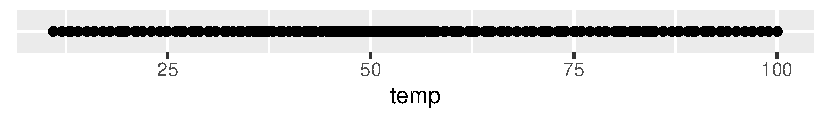
\includegraphics{02-visualization_files/figure-pdf/fig-temp-on-line-1.pdf}

}

\caption{\label{fig-temp-on-line}Plot of Hourly Temperature Recordings
from NYC in 2013}

\end{figure}

This gives us a general idea of how the values of \texttt{temp}
distribute: observe that temperatures vary from around 11°F up to 100°F.
Furthermore, there appear to be more recorded temperatures between 40°F
and 60°F than outside this range. However, because of the high degree of
overlap in the points, it's hard to get a sense of exactly how many
values are between, say, 50°F and 55°F.

What is commonly produced instead of the above plot is known as a
\emph{histogram}. A histogram is a plot that visualizes the
\emph{distribution} of a numerical value as follows:

\begin{enumerate}
\def\labelenumi{\arabic{enumi}.}
\item
  We first cut up the x-axis into a series of \emph{bins}, where each
  bin represents a range of values.
\item
  For each bin, we count the number of observations that fall in the
  range corresponding to that bin.
\item
  Then for each bin, we draw a bar whose height marks the corresponding
  count.
\end{enumerate}

Let's drill-down on an example of a histogram, shown in
@fig-histogramexample.

\begin{figure}

{\centering 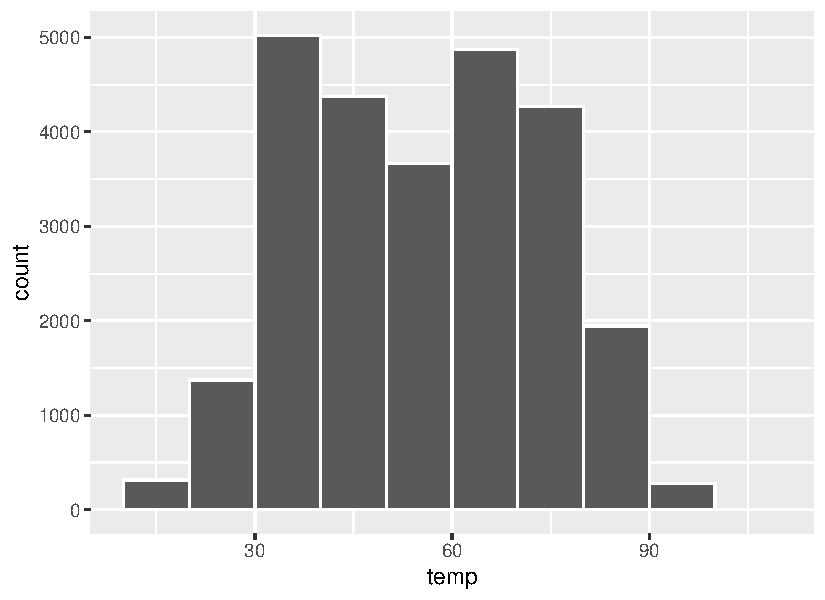
\includegraphics{02-visualization_files/figure-pdf/fig-histogramexample-1.pdf}

}

\caption{\label{fig-histogramexample}Example histogram}

\end{figure}

Observe that there are three bins of equal width between 30°F and 60°F,
thus we have three bins of width 10°F each: one bin for the 30-40°F
range, another bin for the 40-50°F range, and another bin for the
50-60°F range. Since:

\begin{enumerate}
\def\labelenumi{\arabic{enumi}.}
\tightlist
\item
  The bin for the 30-40°F range has a height of around 5000, this
  histogram is telling us that around 5000 of the hourly temperature
  recordings are between 30°F and 40°F.
\item
  The bin for the 40-50°F range has a height of around 4300, this
  histogram is telling us that around 4300 of the hourly temperature
  recordings are between 40°F and 50°F.
\item
  The bin for the 50-60°F range has a height of around 3500, this
  histogram is telling us that around 3500 of the hourly temperature
  recordings are between 50°F and 60°F.
\end{enumerate}

The remaining bins all have a similar interpretation.

\hypertarget{sec-geomhistogram}{%
\subsection{Histograms via geom\_histogram}\label{sec-geomhistogram}}

Let's now present the \texttt{ggplot()} code to plot your first
histogram! Unlike with scatterplots and linegraphs, there is now only
one variable being mapped in \texttt{aes()}: the single numerical
variable \texttt{temp}. The y-aesthetic of a histogram gets computed for
you automatically. Furthermore, the geometric object layer is now a
\texttt{geom\_histogram()}

\begin{Shaded}
\begin{Highlighting}[]
\FunctionTok{ggplot}\NormalTok{(}\AttributeTok{data =}\NormalTok{ weather, }\AttributeTok{mapping =} \FunctionTok{aes}\NormalTok{(}\AttributeTok{x =}\NormalTok{ temp)) }\SpecialCharTok{+}
  \FunctionTok{geom\_histogram}\NormalTok{()}
\end{Highlighting}
\end{Shaded}

\begin{verbatim}
`stat_bin()` using `bins = 30`. Pick better value with `binwidth`.
\end{verbatim}

\begin{verbatim}
Warning: Removed 1 rows containing non-finite values (stat_bin).
\end{verbatim}

\begin{figure}[H]

{\centering 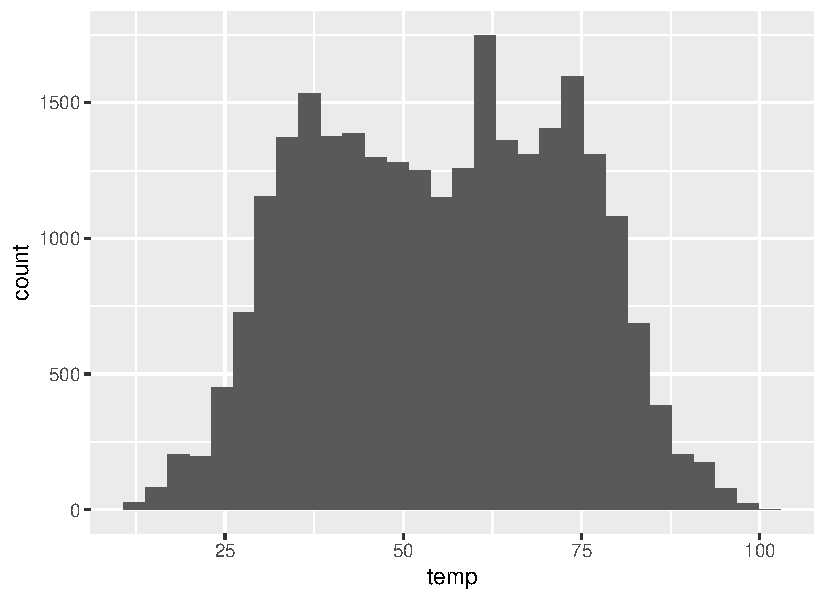
\includegraphics{02-visualization_files/figure-pdf/fig-weather-histogram-1.pdf}

}

\caption{\label{fig-weather-histogram}Histogram of hourly temperatures
at three NYC airports}

\end{figure}

Let's unpack the messages R sent us first. The first message is telling
us that the histogram was constructed using \texttt{bins\ =\ 30}, in
other words 30 equally spaced bins. This is known in computer
programming as a default value; unless you override this default number
of bins with a number you specify, R will choose 30 by default. We'll
see in the next section how to change this default number of bins. The
second message is telling us something similar to the warning message we
received when we ran the code to create a scatterplot of departure and
arrival delays for Alaska Airlines flights in Figure~\ref{fig-noalpha}:
that because one row has a missing \texttt{NA} value for \texttt{temp},
it was omitted from the histogram. R is just giving us a friendly heads
up that this was the case.

Now's let's unpack the resulting histogram in
Figure~\ref{fig-weather-histogram}. Observe that values less than 25°F
as well as values above 80°F are rather rare. However, because of the
large number of bins, its hard to get a sense for which range of
temperatures is covered by each bin; everything is one giant amorphous
blob. So let's add white vertical borders demarcating the bins by adding
a \texttt{color\ =\ "white"} argument to \texttt{geom\_histogram()}:

\begin{Shaded}
\begin{Highlighting}[]
\FunctionTok{ggplot}\NormalTok{(}\AttributeTok{data =}\NormalTok{ weather, }\AttributeTok{mapping =} \FunctionTok{aes}\NormalTok{(}\AttributeTok{x =}\NormalTok{ temp)) }\SpecialCharTok{+}
  \FunctionTok{geom\_histogram}\NormalTok{(}\AttributeTok{color =} \StringTok{"white"}\NormalTok{)}
\end{Highlighting}
\end{Shaded}

\begin{figure}[H]

{\centering 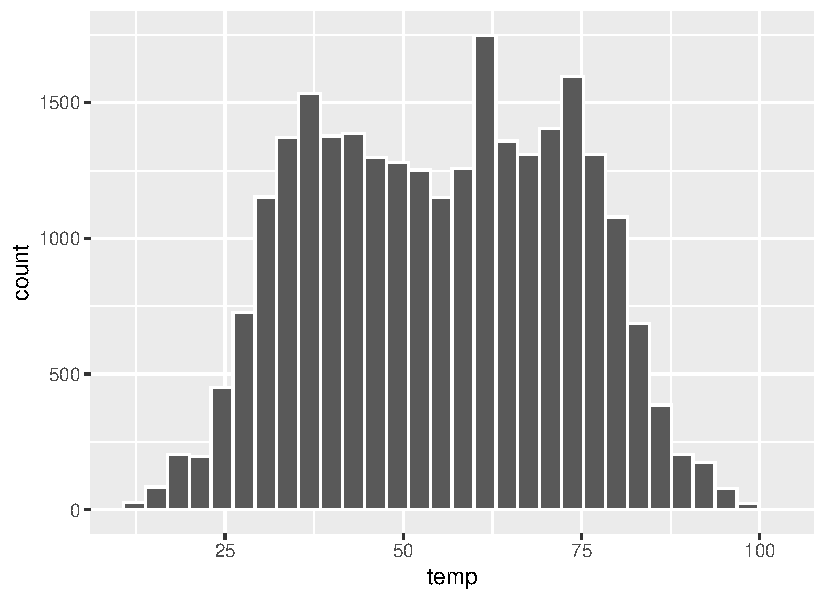
\includegraphics{02-visualization_files/figure-pdf/fig-weather-histogram-2-1.pdf}

}

\caption{\label{fig-weather-histogram-2}Histogram of hourly temperatures
at three NYC airports with white borders}

\end{figure}

We can now better associate ranges of temperatures to each of the bins.
We can also vary the color of the bars by setting the \texttt{fill}
argument. Run \texttt{colors()} to see all 657 possible choice of
colors!

\begin{Shaded}
\begin{Highlighting}[]
\FunctionTok{ggplot}\NormalTok{(}\AttributeTok{data =}\NormalTok{ weather, }\AttributeTok{mapping =} \FunctionTok{aes}\NormalTok{(}\AttributeTok{x =}\NormalTok{ temp)) }\SpecialCharTok{+}
  \FunctionTok{geom\_histogram}\NormalTok{(}\AttributeTok{color =} \StringTok{"white"}\NormalTok{, }\AttributeTok{fill =} \StringTok{"steelblue"}\NormalTok{)}
\end{Highlighting}
\end{Shaded}

\begin{figure}[H]

{\centering 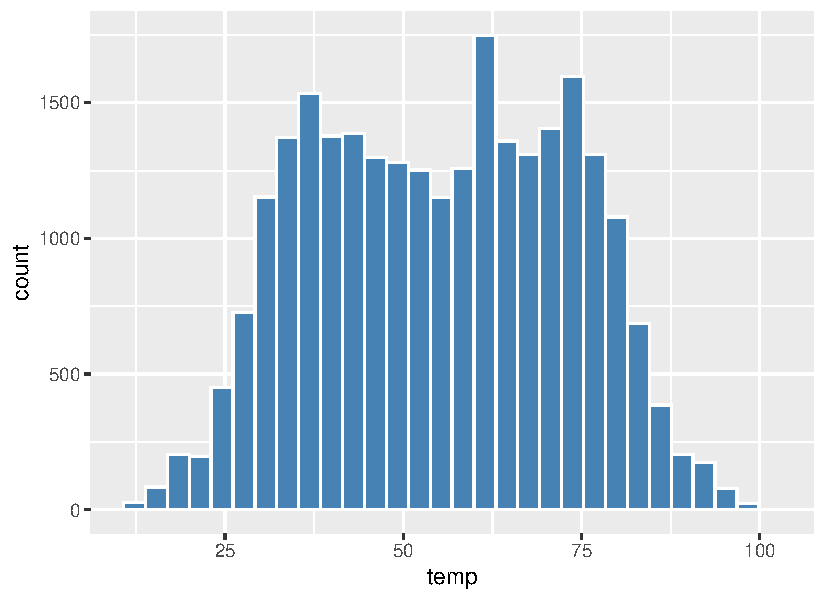
\includegraphics{02-visualization_files/figure-pdf/fig-weather-histogram-3-1.pdf}

}

\caption{\label{fig-weather-histogram-3}Histogram of hourly temperatures
at three NYC airports with white borders}

\end{figure}

\hypertarget{sec-adjustbins}{%
\subsection{Adjusting the bins}\label{sec-adjustbins}}

Observe in both Figure~\ref{fig-weather-histogram-2} and
Figure~\ref{fig-weather-histogram-3} that in the 50-75°F range there
appear to be roughly 8 bins. Thus each bin has width 25 divided by 8, or
roughly 3.12°F which is not a very easily interpretable range to work
with. Let's now adjust the number of bins in our histogram in one of two
methods:

\begin{enumerate}
\def\labelenumi{\arabic{enumi}.}
\tightlist
\item
  By adjusting the number of bins via the \texttt{bins} argument to
  \texttt{geom\_histogram()}.
\item
  By adjusting the width of the bins via the \texttt{binwidth} argument
  to \texttt{geom\_histogram()}.
\end{enumerate}

Using the first method, we have the power to specify how many bins we
would like to cut the x-axis up in. As mentioned in the previous
section, the default number of bins is 30. We can override this default,
to say 40 bins, as follows:

\begin{Shaded}
\begin{Highlighting}[]
\FunctionTok{ggplot}\NormalTok{(}\AttributeTok{data =}\NormalTok{ weather, }\AttributeTok{mapping =} \FunctionTok{aes}\NormalTok{(}\AttributeTok{x =}\NormalTok{ temp)) }\SpecialCharTok{+}
  \FunctionTok{geom\_histogram}\NormalTok{(}\AttributeTok{bins =} \DecValTok{40}\NormalTok{, }\AttributeTok{color =} \StringTok{"white"}\NormalTok{)}
\end{Highlighting}
\end{Shaded}

\begin{figure}[H]

{\centering 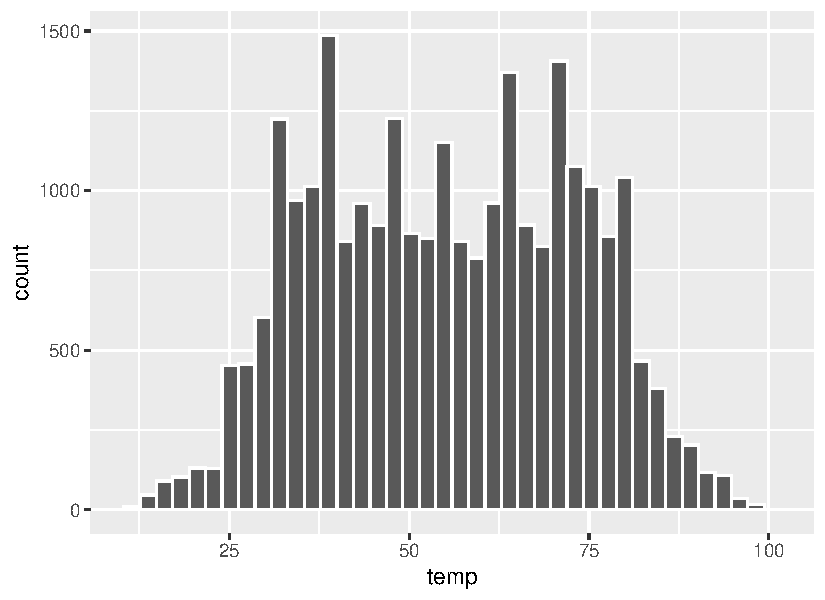
\includegraphics{02-visualization_files/figure-pdf/fig-hist-bins40-1.pdf}

}

\caption{\label{fig-hist-bins40}Histogram with 40 bins}

\end{figure}

Using the second method, instead of specifying the number of bins, we
specify the width of the bins by using the \texttt{binwidth} argument in
the \texttt{geom\_histogram()} layer. For example, let's set the width
of each bin to be 10°F.

\begin{Shaded}
\begin{Highlighting}[]
\FunctionTok{ggplot}\NormalTok{(}\AttributeTok{data =}\NormalTok{ weather, }\AttributeTok{mapping =} \FunctionTok{aes}\NormalTok{(}\AttributeTok{x =}\NormalTok{ temp)) }\SpecialCharTok{+}
  \FunctionTok{geom\_histogram}\NormalTok{(}\AttributeTok{binwidth =} \DecValTok{10}\NormalTok{, }\AttributeTok{color =} \StringTok{"white"}\NormalTok{)}
\end{Highlighting}
\end{Shaded}

\begin{figure}[H]

{\centering 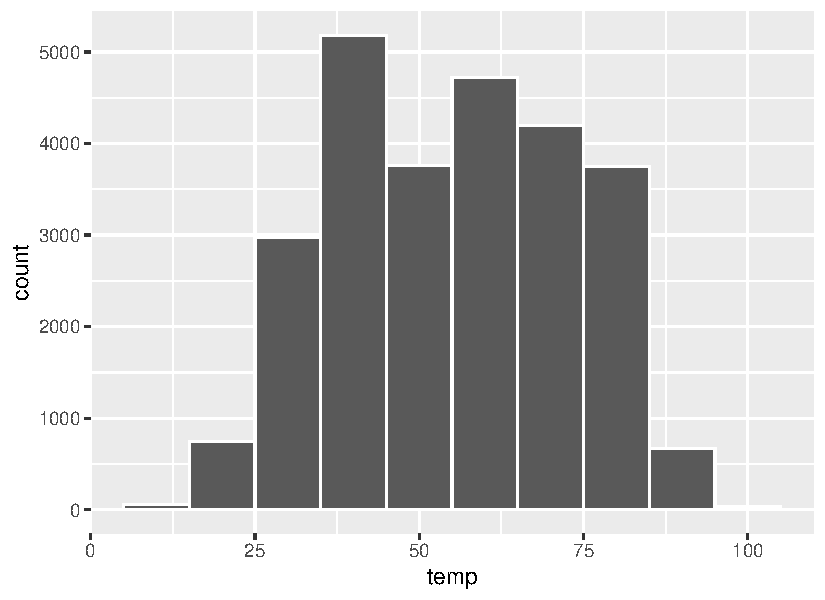
\includegraphics{02-visualization_files/figure-pdf/fig-hist-binwidth10-1.pdf}

}

\caption{\label{fig-hist-binwidth10}Histogram with binwidth 10}

\end{figure}

\begin{tcolorbox}[enhanced jigsaw, coltitle=black, toprule=.15mm, bottomtitle=1mm, breakable, leftrule=.75mm, title={{🎯} Learning Check 2.14}, opacitybacktitle=0.6, colback=white, rightrule=.15mm, opacityback=0, toptitle=1mm, colbacktitle=quarto-callout-tip-color!10!white, colframe=quarto-callout-tip-color-frame, titlerule=0mm, arc=.35mm, bottomrule=.15mm, left=2mm]
What does changing the number of bins from 30 to 40 tell us about the
distribution of temperatures?
\end{tcolorbox}

\begin{tcolorbox}[enhanced jigsaw, coltitle=black, toprule=.15mm, bottomtitle=1mm, breakable, leftrule=.75mm, title={{🎯} Learning Check 2.15}, opacitybacktitle=0.6, colback=white, rightrule=.15mm, opacityback=0, toptitle=1mm, colbacktitle=quarto-callout-tip-color!10!white, colframe=quarto-callout-tip-color-frame, titlerule=0mm, arc=.35mm, bottomrule=.15mm, left=2mm]
Would you classify the distribution of temperatures as symmetric or
skewed?
\end{tcolorbox}

\begin{tcolorbox}[enhanced jigsaw, coltitle=black, toprule=.15mm, bottomtitle=1mm, breakable, leftrule=.75mm, title={{🎯} Learning Check 2.16}, opacitybacktitle=0.6, colback=white, rightrule=.15mm, opacityback=0, toptitle=1mm, colbacktitle=quarto-callout-tip-color!10!white, colframe=quarto-callout-tip-color-frame, titlerule=0mm, arc=.35mm, bottomrule=.15mm, left=2mm]
What would you guess is the ``center'' value in this distribution? Why
did you make that choice?
\end{tcolorbox}

\begin{tcolorbox}[enhanced jigsaw, coltitle=black, toprule=.15mm, bottomtitle=1mm, breakable, leftrule=.75mm, title={{🎯} Learning Check 2.17}, opacitybacktitle=0.6, colback=white, rightrule=.15mm, opacityback=0, toptitle=1mm, colbacktitle=quarto-callout-tip-color!10!white, colframe=quarto-callout-tip-color-frame, titlerule=0mm, arc=.35mm, bottomrule=.15mm, left=2mm]
Is this data spread out greatly from the center or is it close? Why?
\end{tcolorbox}

\hypertarget{summary-2}{%
\subsection{Summary}\label{summary-2}}

Histograms, unlike scatterplots and linegraphs, present information on
only a single numerical variable. Specifically, they are visualizations
of the distribution of the numerical variable in question.

\hypertarget{sec-facets}{%
\section{Facets}\label{sec-facets}}

Before continuing the 5NG, let's briefly introduce a new concept called
\emph{faceting}. Faceting is used when we'd like to split a particular
visualization of variables by another variable. This will create
multiple copies of the same type of plot with matching x and y axes, but
whose content will differ.

For example, suppose we were interested in looking at how the histogram
of hourly temperature recordings at the three NYC airports we saw in
Section~\ref{sec-histograms} differed by month. We would ``split'' this
histogram by the 12 possible months in a given year, in other words plot
histograms of \texttt{temp} for each \texttt{month}. We do this by
adding \texttt{facet\_wrap(\textasciitilde{}\ month)} layer.

\begin{Shaded}
\begin{Highlighting}[]
\FunctionTok{ggplot}\NormalTok{(}\AttributeTok{data =}\NormalTok{ weather, }\AttributeTok{mapping =} \FunctionTok{aes}\NormalTok{(}\AttributeTok{x =}\NormalTok{ temp)) }\SpecialCharTok{+}
  \FunctionTok{geom\_histogram}\NormalTok{(}\AttributeTok{binwidth =} \DecValTok{5}\NormalTok{, }\AttributeTok{color =} \StringTok{"white"}\NormalTok{) }\SpecialCharTok{+}
  \FunctionTok{facet\_wrap}\NormalTok{(}\SpecialCharTok{\textasciitilde{}}\NormalTok{ month)}
\end{Highlighting}
\end{Shaded}

\begin{figure}[H]

{\centering 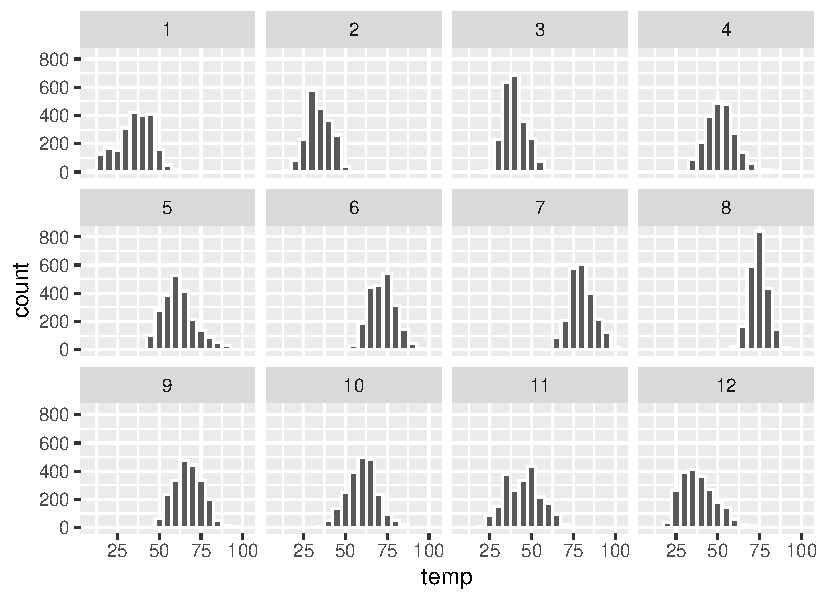
\includegraphics{02-visualization_files/figure-pdf/fig-facethistogram-1.pdf}

}

\caption{\label{fig-facethistogram}Faceted histogram}

\end{figure}

Note the use of the tilde \texttt{\textasciitilde{}} before
\texttt{month} in \texttt{facet\_wrap()}. The tilde is required and
you'll receive the error
\texttt{Error\ in\ as.quoted(facets)\ :\ object\ \textquotesingle{}month\textquotesingle{}\ not\ found}
if you don't include it before \texttt{month} here. We can also specify
the number of rows and columns in the grid by using the \texttt{nrow}
and \texttt{ncol} arguments inside of \texttt{facet\_wrap()}. For
example, say we would like our faceted plot to have 4 rows instead of 3.
Add the \texttt{nrow\ =\ 4} argument to
\texttt{facet\_wrap(\textasciitilde{}\ month)}

\begin{Shaded}
\begin{Highlighting}[]
\FunctionTok{ggplot}\NormalTok{(}\AttributeTok{data =}\NormalTok{ weather, }\AttributeTok{mapping =} \FunctionTok{aes}\NormalTok{(}\AttributeTok{x =}\NormalTok{ temp)) }\SpecialCharTok{+}
  \FunctionTok{geom\_histogram}\NormalTok{(}\AttributeTok{binwidth =} \DecValTok{5}\NormalTok{, }\AttributeTok{color =} \StringTok{"white"}\NormalTok{) }\SpecialCharTok{+}
  \FunctionTok{facet\_wrap}\NormalTok{(}\SpecialCharTok{\textasciitilde{}}\NormalTok{ month, }\AttributeTok{nrow =} \DecValTok{4}\NormalTok{)}
\end{Highlighting}
\end{Shaded}

\begin{figure}[H]

{\centering 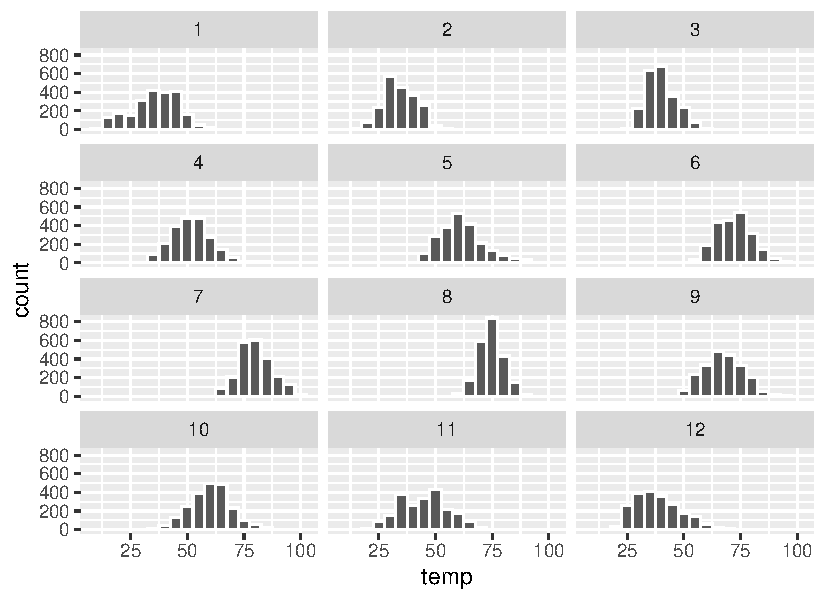
\includegraphics{02-visualization_files/figure-pdf/fig-facethistogram2-1.pdf}

}

\caption{\label{fig-facethistogram2}Faceted histogram with 4 instead of
3 rows}

\end{figure}

Observe in both Figure~\ref{fig-facethistogram} and
Figure~\ref{fig-facethistogram2} that as we might expect in the Northern
Hemisphere, temperatures tend to be higher in the summer months, while
they tend to be lower in the winter.

\begin{tcolorbox}[enhanced jigsaw, coltitle=black, toprule=.15mm, bottomtitle=1mm, breakable, leftrule=.75mm, title={{🎯} Learning Check 2.18}, opacitybacktitle=0.6, colback=white, rightrule=.15mm, opacityback=0, toptitle=1mm, colbacktitle=quarto-callout-tip-color!10!white, colframe=quarto-callout-tip-color-frame, titlerule=0mm, arc=.35mm, bottomrule=.15mm, left=2mm]
What other things do you notice about the faceted plot above? How does a
faceted plot help us see relationships between two variables?
\end{tcolorbox}

\begin{tcolorbox}[enhanced jigsaw, coltitle=black, toprule=.15mm, bottomtitle=1mm, breakable, leftrule=.75mm, title={{🎯} Learning Check 2.19}, opacitybacktitle=0.6, colback=white, rightrule=.15mm, opacityback=0, toptitle=1mm, colbacktitle=quarto-callout-tip-color!10!white, colframe=quarto-callout-tip-color-frame, titlerule=0mm, arc=.35mm, bottomrule=.15mm, left=2mm]
What do the numbers 1-12 correspond to in the plot above? What about 25,
50, 75, 100?
\end{tcolorbox}

\begin{tcolorbox}[enhanced jigsaw, coltitle=black, toprule=.15mm, bottomtitle=1mm, breakable, leftrule=.75mm, title={{🎯} Learning Check 2.20}, opacitybacktitle=0.6, colback=white, rightrule=.15mm, opacityback=0, toptitle=1mm, colbacktitle=quarto-callout-tip-color!10!white, colframe=quarto-callout-tip-color-frame, titlerule=0mm, arc=.35mm, bottomrule=.15mm, left=2mm]
For which types of data sets would these types of faceted plots not work
well in comparing relationships between variables? Give an example
describing the nature of these variables and other important
characteristics.
\end{tcolorbox}

\begin{tcolorbox}[enhanced jigsaw, coltitle=black, toprule=.15mm, bottomtitle=1mm, breakable, leftrule=.75mm, title={{🎯} Learning Check 2.21}, opacitybacktitle=0.6, colback=white, rightrule=.15mm, opacityback=0, toptitle=1mm, colbacktitle=quarto-callout-tip-color!10!white, colframe=quarto-callout-tip-color-frame, titlerule=0mm, arc=.35mm, bottomrule=.15mm, left=2mm]
Does the \texttt{temp} variable in the \texttt{weather} data set have a
lot of variability? Why do you say that?
\end{tcolorbox}

\hypertarget{sec-boxplots}{%
\section{5NG\#4: Boxplots}\label{sec-boxplots}}

While faceted histograms are one visualization that allows us to compare
distributions of a numerical variable split by another variable, another
visualization that achieves this same goal are \emph{side-by-side
boxplots}. A boxplot is constructed from the information provided in the
\emph{five-number summary} of a numerical variable (see
Appendix~\ref{sec-stat-background}). To keep things simple for now,
let's only consider hourly temperature recordings for the month of
November in Figure~\ref{fig-nov1}.

\begin{figure}

{\centering 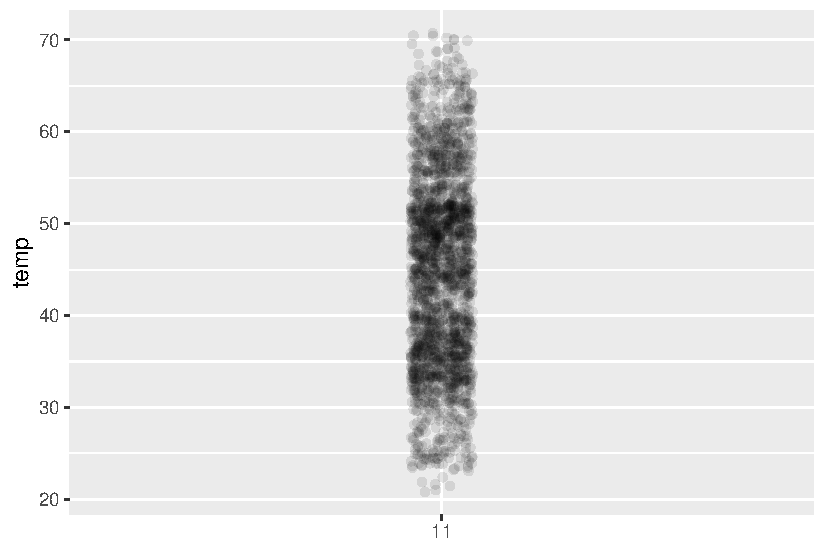
\includegraphics{02-visualization_files/figure-pdf/fig-nov1-1.pdf}

}

\caption{\label{fig-nov1}November temperatures}

\end{figure}

These 2141 observations have the following five-number summary:

\begin{enumerate}
\def\labelenumi{\arabic{enumi}.}
\tightlist
\item
  Minimum: 21.02°F
\item
  First quartile AKA 25\textsuperscript{th} percentile: 35.96°F
\item
  Median AKA second quartile AKA 50\textsuperscript{th} percentile:
  44.96°F
\item
  Third quartile AKA 75\textsuperscript{th} percentile: 51.98°F
\item
  Maximum: 71.06°F
\end{enumerate}

Let's mark these 5 values with dashed horizontal lines in
Figure~\ref{fig-nov2}.

\begin{figure}

{\centering 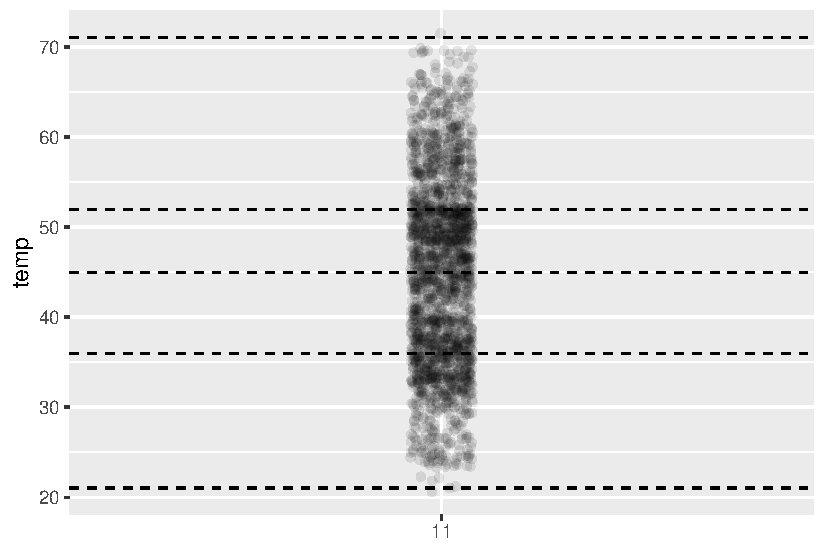
\includegraphics{02-visualization_files/figure-pdf/fig-nov2-1.pdf}

}

\caption{\label{fig-nov2}November temperatures}

\end{figure}

Let's add the boxplot underneath these points and dashed horizontal
lines in Figure~\ref{fig-nov3}.

\begin{figure}

{\centering 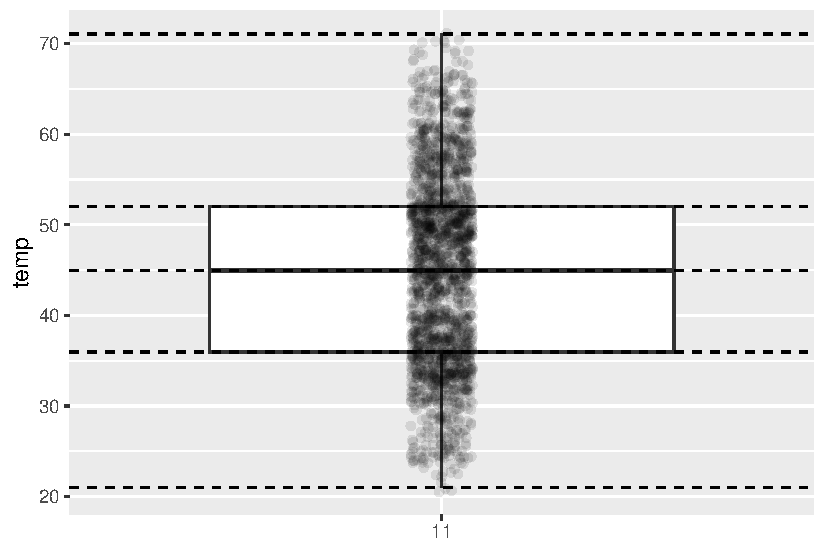
\includegraphics{02-visualization_files/figure-pdf/fig-nov3-1.pdf}

}

\caption{\label{fig-nov3}November temperatures}

\end{figure}

What the boxplot does summarize the 2141 points by emphasizing that:

\begin{enumerate}
\def\labelenumi{\arabic{enumi}.}
\item
  25\% of points (about 534 observations) fall below the bottom edge of
  the box, which is the first quartile of 35.96°F. In other words 25\%
  of observations were colder than 35.96°F.
\item
  25\% of points fall between the bottom edge of the box and the solid
  middle line, which is the median of 44.96°F. In other words 25\% of
  observations were between 35.96 and 44.96°F and 50\% of observations
  were colder than 44.96°F.
\item
  25\% of points fall between the solid middle line and the top edge of
  the box, which is the third quartile of 51.98°F. In other words 25\%
  of observations were between 44.96 and 51.98°F and 75\% of
  observations were colder than 51.98°F.
\item
  25\% of points fall over the top edge of the box. In other words 25\%
  of observations were warmer than 51.98°F.
\item
  The middle 50\% of points lie within the \emph{interquartile range}
  between the first and third quartile of 51.98 - 35.96 = 16.02°F.
\end{enumerate}

Lastly, for clarity's sake let's remove the points but keep the dashed
horizontal lines in Figure~\ref{fig-nov4}.

\begin{figure}

{\centering 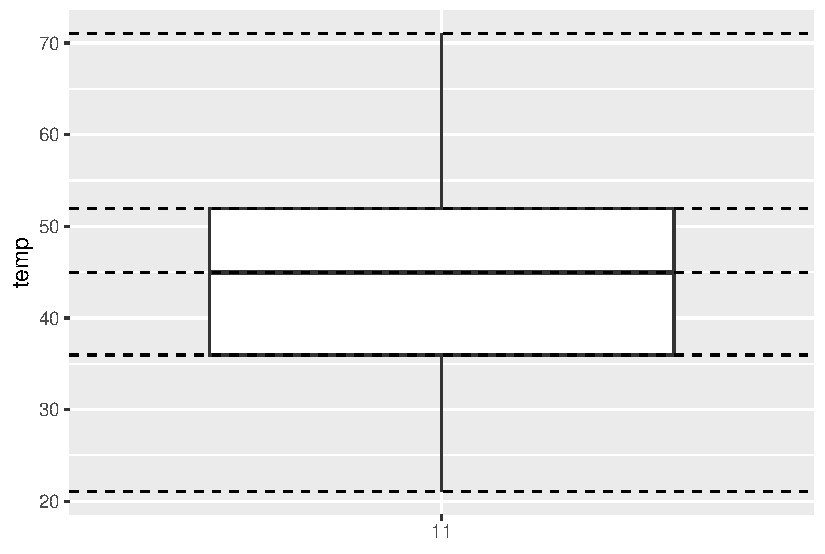
\includegraphics{02-visualization_files/figure-pdf/fig-nov4-1.pdf}

}

\caption{\label{fig-nov4}November temperatures}

\end{figure}

We can now better see the \emph{whiskers} of the boxplot. They stick out
from either end of the box all the way to the minimum and maximum
observed temperatures of 21.02°F and 71.06°F respectively. However, the
whiskers don't always extend to the smallest and largest observed
values. They in fact can extend no more than 1.5 \(\times\) the
interquartile range from either end of the box, in this case 1.5
\(\times\) 16.02°F = 24.03°F from either end of the box. Any observed
values outside this whiskers get marked with points called
\emph{outliers}, which we'll see in the next section.

\hypertarget{sec-geomboxplot}{%
\subsection{Boxplots via geom\_boxplot}\label{sec-geomboxplot}}

Let's now create a side-by-side boxplot of hourly temperatures split by
the 12 months as we did above with the faceted histograms. We do this by
mapping the \texttt{month} variable to the x-position aesthetic, the
\texttt{temp} variable to the y-position aesthetic, and by adding a
\texttt{geom\_boxplot()} layer:

\begin{Shaded}
\begin{Highlighting}[]
\FunctionTok{ggplot}\NormalTok{(}\AttributeTok{data =}\NormalTok{ weather, }\AttributeTok{mapping =} \FunctionTok{aes}\NormalTok{(}\AttributeTok{x =}\NormalTok{ month, }\AttributeTok{y =}\NormalTok{ temp)) }\SpecialCharTok{+}
  \FunctionTok{geom\_boxplot}\NormalTok{()}
\end{Highlighting}
\end{Shaded}

\begin{figure}[H]

{\centering 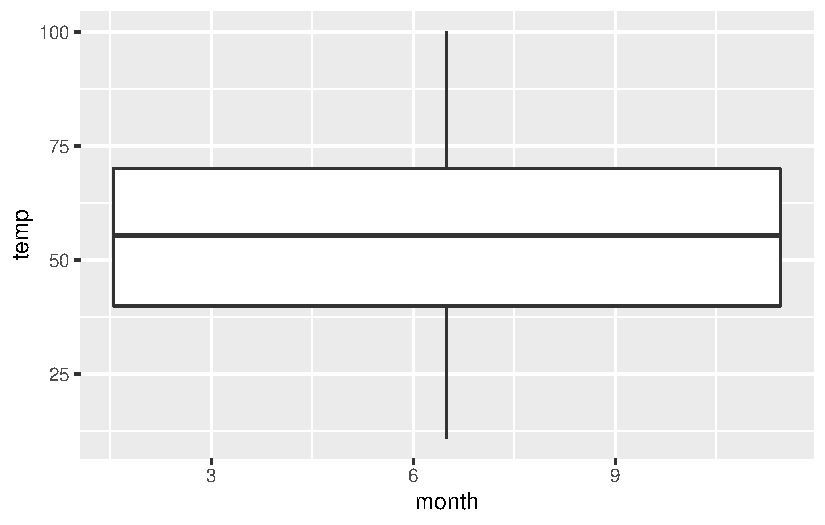
\includegraphics{02-visualization_files/figure-pdf/fig-badbox-1.pdf}

}

\caption{\label{fig-badbox}Invalid boxplot specification}

\end{figure}

\begin{verbatim}
Warning messages:
1: Continuous x aesthetic -- did you forget aes(group=...)? 
2: Removed 1 rows containing non-finite values (stat_boxplot). 
\end{verbatim}

Observe in Figure~\ref{fig-badbox} that this plot does not provide
information about temperature separated by month. The warning messages
clue us in as to why. The second warning message is identical to the
warning message when plotting a histogram of hourly temperatures: that
one of the values was recorded as \texttt{NA} missing. However, the
first warning message is telling us that we have a ``continuous'', or
numerical variable, on the x-position aesthetic. Boxplots however
require a categorical variable on the x-axis.

We can convert the numerical variable \texttt{month} into a categorical
variable by using the \texttt{factor()} function. So after applying
\texttt{factor(month)}, month goes from having numerical values 1, 2,
\ldots, 12 to having labels ``1'', ``2'', \ldots, ``12.''

\begin{Shaded}
\begin{Highlighting}[]
\FunctionTok{ggplot}\NormalTok{(}\AttributeTok{data =}\NormalTok{ weather, }\AttributeTok{mapping =} \FunctionTok{aes}\NormalTok{(}\AttributeTok{x =} \FunctionTok{factor}\NormalTok{(month), }\AttributeTok{y =}\NormalTok{ temp)) }\SpecialCharTok{+}
  \FunctionTok{geom\_boxplot}\NormalTok{()}
\end{Highlighting}
\end{Shaded}

\begin{figure}[H]

{\centering 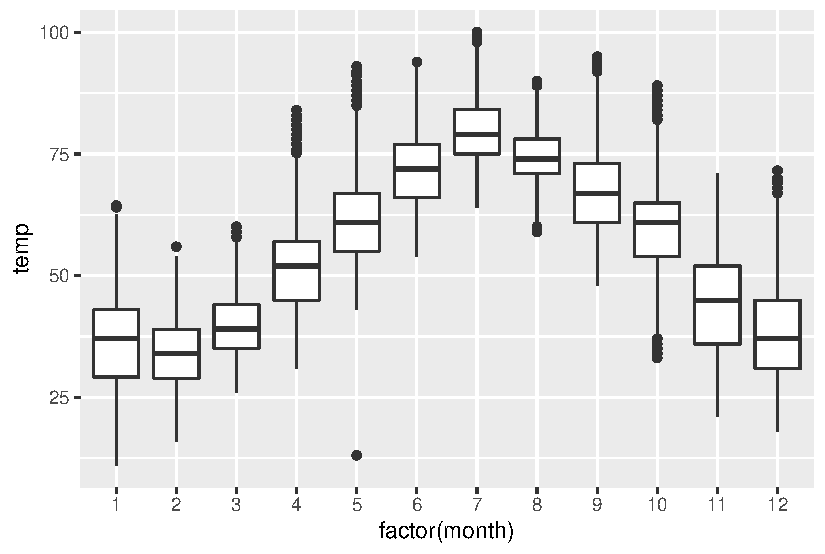
\includegraphics{02-visualization_files/figure-pdf/fig-monthtempbox-1.pdf}

}

\caption{\label{fig-monthtempbox}Temp by month boxplot}

\end{figure}

The resulting Figure~\ref{fig-monthtempbox} shows 12 separate ``box and
whiskers'' plots with the features we saw earlier focusing only on
November:

\begin{itemize}
\item
  The ``box'' portions of this visualization represent the
  1\textsuperscript{st} quartile, the median AKA the
  2\textsuperscript{nd} quartile, and the 3\textsuperscript{rd}
  quartile.
\item
  The ``length'' of each box, i.e.~the value of the
  3\textsuperscript{rd} quartile minus the value of the
  1\textsuperscript{st} quartile, is the \emph{interquartile range}. It
  is a measure of spread of the middle 50\% of values, with longer boxes
  indicating more variability.
\item
  The ``whisker'' portions of these plots extend out from the bottoms
  and tops of the boxes and represent points less than the
  25\textsuperscript{th} percentile and greater than the
  75\textsuperscript{th} percentiles respectively. They're set to extend
  out no more than \(1.5 \times IQR\) units away from either end of the
  boxes. We say ``no more than'' because the ends of the whiskers have
  to correspond to observed temperatures. The length of these whiskers
  show how the data outside the middle 50\% of values vary, with longer
  whiskers indicating more variability.
\item
  The dots representing values falling outside the whiskers are called
  \emph{outliers}. These can be thought of as anomalous values.
\end{itemize}

It is important to keep in mind that the definition of an outlier is
somewhat arbitrary and not absolute. In this case, they are defined by
the length of the whiskers, which are no more than \(1.5 \times IQR\)
units long. Looking at this plot we can see, as expected, that summer
months (6 through 8) have higher median temperatures as evidenced by the
higher solid lines in the middle of the boxes. We can easily compare
temperatures across months by drawing imaginary horizontal lines across
the plot. Furthermore, the height of the 12 boxes as quantified by the
interquartile ranges are informative too; they tell us about
variability, or spread, of temperatures recorded in a given month.

\begin{tcolorbox}[enhanced jigsaw, coltitle=black, toprule=.15mm, bottomtitle=1mm, breakable, leftrule=.75mm, title={{🎯} Learning Check 2.22}, opacitybacktitle=0.6, colback=white, rightrule=.15mm, opacityback=0, toptitle=1mm, colbacktitle=quarto-callout-tip-color!10!white, colframe=quarto-callout-tip-color-frame, titlerule=0mm, arc=.35mm, bottomrule=.15mm, left=2mm]
What does the dot at the bottom of the plot for May correspond to?
Explain what might have occurred in May to produce this point.
\end{tcolorbox}

\begin{tcolorbox}[enhanced jigsaw, coltitle=black, toprule=.15mm, bottomtitle=1mm, breakable, leftrule=.75mm, title={{🎯} Learning Check 2.23}, opacitybacktitle=0.6, colback=white, rightrule=.15mm, opacityback=0, toptitle=1mm, colbacktitle=quarto-callout-tip-color!10!white, colframe=quarto-callout-tip-color-frame, titlerule=0mm, arc=.35mm, bottomrule=.15mm, left=2mm]
Which months have the highest variability in temperature? What reasons
can you give for this?
\end{tcolorbox}

\begin{tcolorbox}[enhanced jigsaw, coltitle=black, toprule=.15mm, bottomtitle=1mm, breakable, leftrule=.75mm, title={{🎯} Learning Check 2.24}, opacitybacktitle=0.6, colback=white, rightrule=.15mm, opacityback=0, toptitle=1mm, colbacktitle=quarto-callout-tip-color!10!white, colframe=quarto-callout-tip-color-frame, titlerule=0mm, arc=.35mm, bottomrule=.15mm, left=2mm]
We looked at the distribution of the numerical variable \texttt{temp}
split by the numerical variable \texttt{month} that we converted to a
categorical variable using the \texttt{factor()} function. Why would a
boxplot of \texttt{temp} split by the numerical variable
\texttt{pressure} similarly converted to a categorical variable using
the \texttt{factor()} not be informative?
\end{tcolorbox}

\begin{tcolorbox}[enhanced jigsaw, coltitle=black, toprule=.15mm, bottomtitle=1mm, breakable, leftrule=.75mm, title={{🎯} Learning Check 2.25}, opacitybacktitle=0.6, colback=white, rightrule=.15mm, opacityback=0, toptitle=1mm, colbacktitle=quarto-callout-tip-color!10!white, colframe=quarto-callout-tip-color-frame, titlerule=0mm, arc=.35mm, bottomrule=.15mm, left=2mm]
Boxplots provide a simple way to identify outliers. Why may outliers be
easier to identify when looking at a boxplot instead of a faceted
histogram?
\end{tcolorbox}

\hypertarget{summary-3}{%
\subsection{Summary}\label{summary-3}}

Side-by-side boxplots provide us with a way to compare and contrast the
distribution of a quantitative variable across multiple levels of
another categorical variable. One can see where the median falls across
the different groups by looking at the center line in the boxes. To see
how spread out the variable is across the different groups, look at both
the width of the box and also how far the whiskers stretch out away from
the box. Outliers are even more easily identified when looking at a
boxplot than when looking at a histogram as they are marked with points.

\hypertarget{sec-geombar}{%
\section{5NG\#5: Barplots}\label{sec-geombar}}

Both histograms and boxplots are tools to visualize the distribution of
numerical variables. Another common task is visualize the distribution
of a categorical variable. This is a simpler task, as we are simply
counting different categories, also known as \emph{levels}, of a
categorical variable. Often the best way to visualize these different
counts, also known as \emph{frequencies}, is with a barplot (also known
as a barchart). One complication, however, is how your data is
represented: is the categorical variable of interest ``pre-counted'' or
not? For example, run the following code that manually creates two data
frames representing a collection of fruit: 3 apples and 2 oranges.

\begin{Shaded}
\begin{Highlighting}[]
\NormalTok{fruits }\OtherTok{\textless{}{-}} \FunctionTok{tibble}\NormalTok{(}
  \AttributeTok{fruit =} \FunctionTok{c}\NormalTok{(}\StringTok{"apple"}\NormalTok{, }\StringTok{"apple"}\NormalTok{, }\StringTok{"orange"}\NormalTok{, }\StringTok{"apple"}\NormalTok{, }\StringTok{"orange"}\NormalTok{)}
\NormalTok{  )}

\NormalTok{fruits\_counted }\OtherTok{\textless{}{-}} \FunctionTok{tibble}\NormalTok{(}
  \AttributeTok{fruit =} \FunctionTok{c}\NormalTok{(}\StringTok{"apple"}\NormalTok{, }\StringTok{"orange"}\NormalTok{),}
  \AttributeTok{number =} \FunctionTok{c}\NormalTok{(}\DecValTok{3}\NormalTok{, }\DecValTok{2}\NormalTok{)}
\NormalTok{  )}
\end{Highlighting}
\end{Shaded}

We see both the \texttt{fruits} and \texttt{fruits\_counted} data frames
represent the same collection of fruit. Whereas \texttt{fruits} just
lists the fruit individually\ldots{}

\begin{verbatim}
# A tibble: 5 x 1
  fruit 
  <chr> 
1 apple 
2 apple 
3 orange
4 apple 
5 orange
\end{verbatim}

\ldots{} \texttt{fruits\_counted} has a variable \texttt{number} which
represents pre-counted values of each fruit.

\begin{verbatim}
# A tibble: 2 x 2
  fruit  number
  <chr>   <dbl>
1 apple       3
2 orange      2
\end{verbatim}

Depending on how your categorical data is represented, you'll need to
use add a different \texttt{geom} layer to your \texttt{ggplot()} to
create a barplot, as we now explore.

\hypertarget{barplots-via-geom_bar-or-geom_col}{%
\subsection{Barplots via geom\_bar or
geom\_col}\label{barplots-via-geom_bar-or-geom_col}}

Let's generate barplots using these two different representations of the
same basket of fruit: 3 apples and 2 oranges. Using the \texttt{fruits}
data frame where all 5 fruits are listed individually in 5 rows, we map
the \texttt{fruit} variable to the x-position aesthetic and add a
\texttt{geom\_bar()} layer.

\begin{Shaded}
\begin{Highlighting}[]
\FunctionTok{ggplot}\NormalTok{(}\AttributeTok{data =}\NormalTok{ fruits, }\AttributeTok{mapping =} \FunctionTok{aes}\NormalTok{(}\AttributeTok{x =}\NormalTok{ fruit)) }\SpecialCharTok{+}
  \FunctionTok{geom\_bar}\NormalTok{()}
\end{Highlighting}
\end{Shaded}

\begin{figure}[H]

{\centering 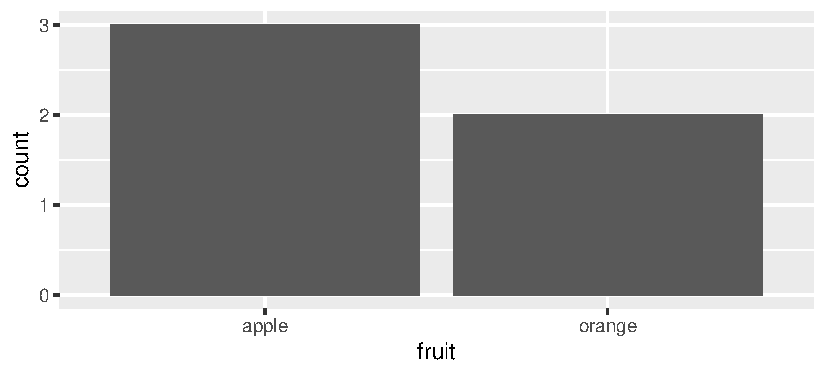
\includegraphics{02-visualization_files/figure-pdf/fig-geombar-1.pdf}

}

\caption{\label{fig-geombar}Barplot when counts are not pre-counted}

\end{figure}

However, using the \texttt{fruits\_counted} data frame where the fruit
have been ``pre-counted'', we map the \texttt{fruit} variable to the
x-position aesthetic as with \texttt{geom\_bar()}, but we also map the
\texttt{count} variable to the y-position aesthetic, and add a
\texttt{geom\_col()} layer.

\begin{Shaded}
\begin{Highlighting}[]
\FunctionTok{ggplot}\NormalTok{(}\AttributeTok{data =}\NormalTok{ fruits\_counted, }\AttributeTok{mapping =} \FunctionTok{aes}\NormalTok{(}\AttributeTok{x =}\NormalTok{ fruit, }\AttributeTok{y =}\NormalTok{ number)) }\SpecialCharTok{+}
  \FunctionTok{geom\_col}\NormalTok{()}
\end{Highlighting}
\end{Shaded}

\begin{figure}[H]

{\centering 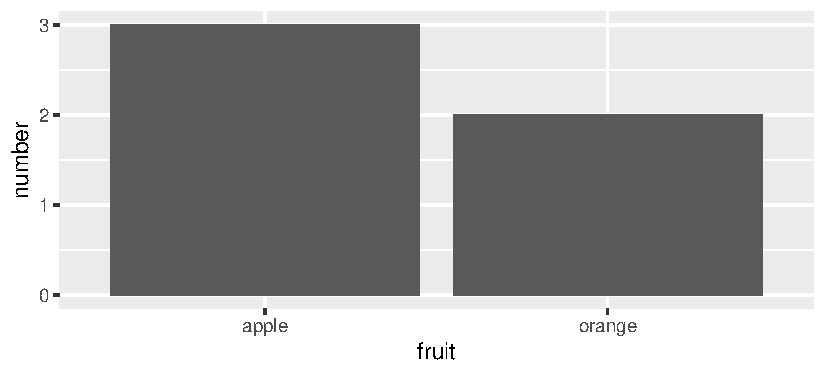
\includegraphics{02-visualization_files/figure-pdf/fig-geomcol-1.pdf}

}

\caption{\label{fig-geomcol}Barplot when counts are pre-counted}

\end{figure}

Compare the barplots in Figure~\ref{fig-geombar} and
Figure~\ref{fig-geomcol}. They are identical because they reflect count
of the same 5 fruit. However depending on how our data is saved, either
pre-counted or not, we must add a different \texttt{geom} layer. When
the categorical variable whose distribution you want to visualize is:

\begin{itemize}
\tightlist
\item
  Is not pre-counted in your data frame: use \texttt{geom\_bar()}.
\item
  Is pre-counted in your data frame, use \texttt{geom\_col()} with the
  y-position aesthetic mapped to the variable that has the counts.
\end{itemize}

Let's now go back to the \texttt{flights} data frame in the
\texttt{nycflights13} package and visualize the distribution of the
categorical variable \texttt{carrier}. In other words, let's visualize
the number of domestic flights out of the three New York City airports
each airline company flew in 2013. Recall from
Section~\ref{sec-exploredataframes} when you first explored the
\texttt{flights} data frame you saw that each row corresponds to a
flight. In other words the \texttt{flights} data frame is more like the
\texttt{fruits} data frame than the \texttt{fruits\_counted} data frame
above, and thus we should use \texttt{geom\_bar()} instead of
\texttt{geom\_col()} to create a barplot. Much like a
\texttt{geom\_histogram()}, there is only one variable in the
\texttt{aes()} aesthetic mapping: the variable \texttt{carrier} gets
mapped to the \texttt{x}-position.

\begin{Shaded}
\begin{Highlighting}[]
\FunctionTok{ggplot}\NormalTok{(}\AttributeTok{data =}\NormalTok{ flights, }\AttributeTok{mapping =} \FunctionTok{aes}\NormalTok{(}\AttributeTok{x =}\NormalTok{ carrier)) }\SpecialCharTok{+}
  \FunctionTok{geom\_bar}\NormalTok{()}
\end{Highlighting}
\end{Shaded}

\begin{figure}[H]

{\centering 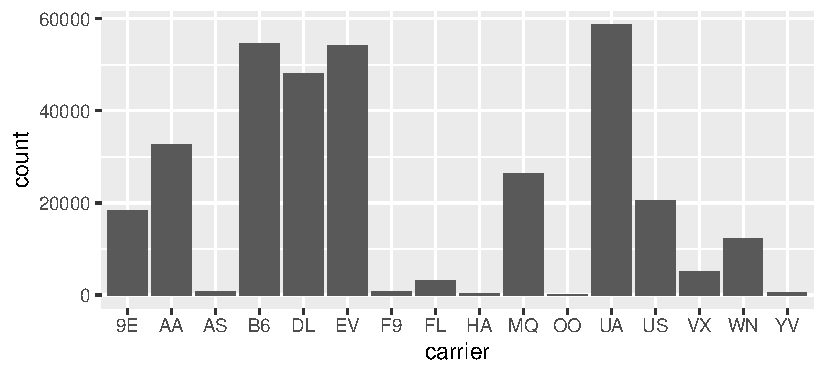
\includegraphics{02-visualization_files/figure-pdf/fig-flightsbar-1.pdf}

}

\caption{\label{fig-flightsbar}Number of flights departing NYC in 2013
by airline using \texttt{geom\_bar()}}

\end{figure}

Observe in Figure~\ref{fig-flightsbar} that United Air Lines
(\texttt{UA}), JetBlue Airways (\texttt{B6}), and ExpressJet Airlines
(\texttt{EV}) had the most flights depart New York City in 2013. If you
don't know which airlines correspond to which carrier codes, then run
\texttt{View(airlines)} to see a directory of airlines. For example: AA
is American Airlines; B6 is JetBlue Airways; DL is Delta Airlines; EV is
ExpressJet Airlines; MQ is Envoy Air; while UA is United Airlines.

Alternatively, say you had a data frame \texttt{flights\_counted} where
the number of flights for each \texttt{carrier} was pre-counted like in
Table~\ref{tbl-flights-counted}.

\hypertarget{tbl-flights-counted}{}
\begin{longtable}[]{@{}lr@{}}
\caption{\label{tbl-flights-counted}Number of flights pre-counted for
each carrier}\tabularnewline
\toprule()
carrier & number \\
\midrule()
\endfirsthead
\toprule()
carrier & number \\
\midrule()
\endhead
UA & 58665 \\
B6 & 54635 \\
EV & 54173 \\
DL & 48110 \\
AA & 32729 \\
MQ & 26397 \\
US & 20536 \\
9E & 18460 \\
WN & 12275 \\
VX & 5162 \\
FL & 3260 \\
AS & 714 \\
F9 & 685 \\
YV & 601 \\
HA & 342 \\
OO & 32 \\
\bottomrule()
\end{longtable}

In order to create a barplot visualizing the distribution of the
categorical variable \texttt{carrier} in this case, we would use
\texttt{geom\_col()} instead with \texttt{x} mapped to \texttt{carrier}
and \texttt{y} mapped to \texttt{number} as seen below. The resulting
barplot would be identical to Figure~\ref{fig-flightsbar}.

\begin{Shaded}
\begin{Highlighting}[]
\FunctionTok{ggplot}\NormalTok{(}\AttributeTok{data =}\NormalTok{ flights\_table, }\AttributeTok{mapping =} \FunctionTok{aes}\NormalTok{(}\AttributeTok{x =}\NormalTok{ carrier, }\AttributeTok{y =}\NormalTok{ number)) }\SpecialCharTok{+}
  \FunctionTok{geom\_col}\NormalTok{()}
\end{Highlighting}
\end{Shaded}

\begin{tcolorbox}[enhanced jigsaw, coltitle=black, toprule=.15mm, bottomtitle=1mm, breakable, leftrule=.75mm, title={{🎯} Learning Check 2.26}, opacitybacktitle=0.6, colback=white, rightrule=.15mm, opacityback=0, toptitle=1mm, colbacktitle=quarto-callout-tip-color!10!white, colframe=quarto-callout-tip-color-frame, titlerule=0mm, arc=.35mm, bottomrule=.15mm, left=2mm]
Why are histograms inappropriate for visualizing categorical variables?
\end{tcolorbox}

\begin{tcolorbox}[enhanced jigsaw, coltitle=black, toprule=.15mm, bottomtitle=1mm, breakable, leftrule=.75mm, title={{🎯} Learning Check 2.27}, opacitybacktitle=0.6, colback=white, rightrule=.15mm, opacityback=0, toptitle=1mm, colbacktitle=quarto-callout-tip-color!10!white, colframe=quarto-callout-tip-color-frame, titlerule=0mm, arc=.35mm, bottomrule=.15mm, left=2mm]
What is the difference between histograms and barplots?
\end{tcolorbox}

\begin{tcolorbox}[enhanced jigsaw, coltitle=black, toprule=.15mm, bottomtitle=1mm, breakable, leftrule=.75mm, title={{🎯} Learning Check 2.28}, opacitybacktitle=0.6, colback=white, rightrule=.15mm, opacityback=0, toptitle=1mm, colbacktitle=quarto-callout-tip-color!10!white, colframe=quarto-callout-tip-color-frame, titlerule=0mm, arc=.35mm, bottomrule=.15mm, left=2mm]
How many Envoy Air flights departed NYC in 2013?
\end{tcolorbox}

\begin{tcolorbox}[enhanced jigsaw, coltitle=black, toprule=.15mm, bottomtitle=1mm, breakable, leftrule=.75mm, title={{🎯} Learning Check 2.29}, opacitybacktitle=0.6, colback=white, rightrule=.15mm, opacityback=0, toptitle=1mm, colbacktitle=quarto-callout-tip-color!10!white, colframe=quarto-callout-tip-color-frame, titlerule=0mm, arc=.35mm, bottomrule=.15mm, left=2mm]
What was the seventh highest airline in terms of departed flights from
NYC in 2013? How could we better present the table to get this answer
quickly?
\end{tcolorbox}

\hypertarget{must-avoid-pie-charts}{%
\subsection{Must avoid pie charts!}\label{must-avoid-pie-charts}}

Unfortunately, one of the most common plots seen today for categorical
data is the pie chart. While they may seem harmless enough, they
actually present a problem in that humans are unable to judge angles
well. As Naomi Robbins describes in her book ``Creating More Effective
Graphs'' (Robbins 2013), we overestimate angles greater than 90 degrees
and we underestimate angles less than 90 degrees. In other words, it is
difficult for us to determine relative size of one piece of the pie
compared to another.

Let's examine the same data used in our previous barplot of the number
of flights departing NYC by airline in Figure~\ref{fig-flightsbar}, but
this time we will use a pie chart in Figure~\ref{fig-carrierpie}.

\begin{figure}

{\centering 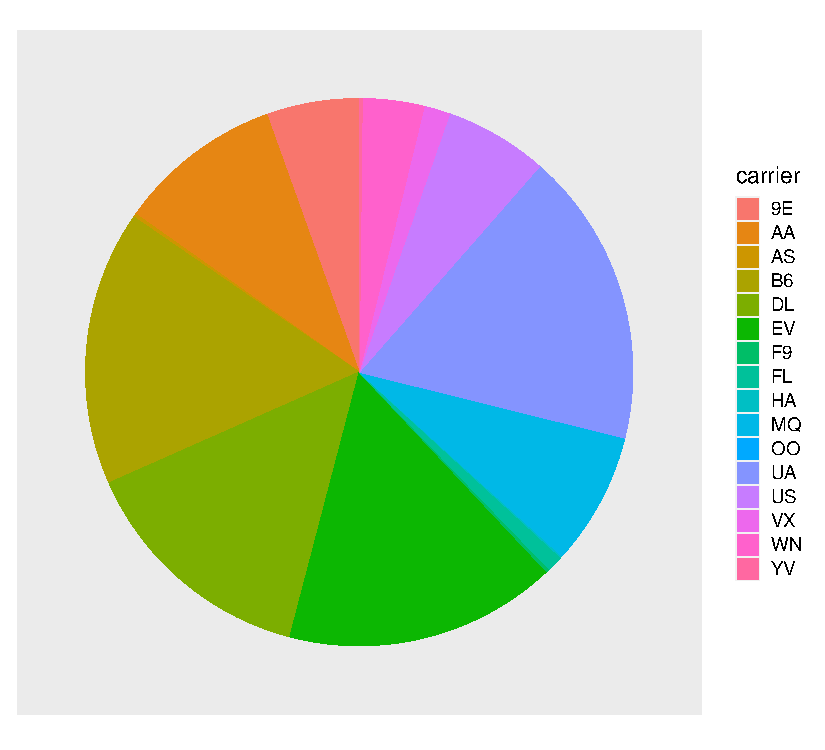
\includegraphics{02-visualization_files/figure-pdf/fig-carrierpie-1.pdf}

}

\caption{\label{fig-carrierpie}The dreaded pie chart}

\end{figure}

Try to answer the following questions:

\begin{itemize}
\tightlist
\item
  How much larger the portion of the pie is for ExpressJet Airlines
  (\texttt{EV}) compared to US Airways (\texttt{US}),
\item
  What the third largest carrier is in terms of departing flights, and
\item
  How many carriers have fewer flights than United Airlines
  (\texttt{UA})?
\end{itemize}

While it is quite difficult to answer these questions when looking at
the pie chart in Figure~\ref{fig-carrierpie}, we can much more easily
answer these questions using the barchart in Figure
Figure~\ref{fig-flightsbar}. This is true since barplots present the
information in a way such that comparisons between categories can be
made with single horizontal lines, whereas pie charts present the
information in a way such that comparisons between categories must be
made by comparing angles.

There may be one exception of a pie chart not to avoid courtesy Nathan
Yau at
\href{https://flowingdata.com/2008/09/19/pie-i-have-eaten-and-pie-i-have-not-eaten/}{FlowingData.com},
but we will leave this for the reader to decide:

\begin{figure}

{\centering 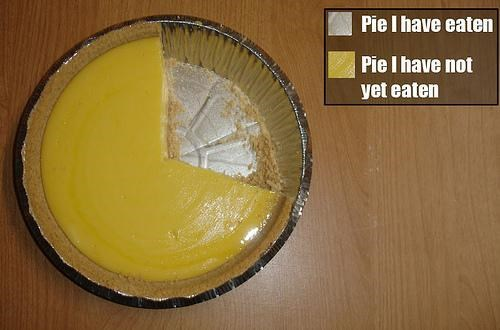
\includegraphics[width=3.79in,height=\textheight]{images/Pie-I-have-Eaten.jpg}

}

\caption{The only good pie chart}

\end{figure}

\begin{tcolorbox}[enhanced jigsaw, coltitle=black, toprule=.15mm, bottomtitle=1mm, breakable, leftrule=.75mm, title={{🎯} Learning Check 2.30}, opacitybacktitle=0.6, colback=white, rightrule=.15mm, opacityback=0, toptitle=1mm, colbacktitle=quarto-callout-tip-color!10!white, colframe=quarto-callout-tip-color-frame, titlerule=0mm, arc=.35mm, bottomrule=.15mm, left=2mm]
Why should pie charts be avoided and replaced by barplots?
\end{tcolorbox}

\begin{tcolorbox}[enhanced jigsaw, coltitle=black, toprule=.15mm, bottomtitle=1mm, breakable, leftrule=.75mm, title={{🎯} Learning Check 2.31}, opacitybacktitle=0.6, colback=white, rightrule=.15mm, opacityback=0, toptitle=1mm, colbacktitle=quarto-callout-tip-color!10!white, colframe=quarto-callout-tip-color-frame, titlerule=0mm, arc=.35mm, bottomrule=.15mm, left=2mm]
Why do you think people continue to use pie charts?
\end{tcolorbox}

\hypertarget{sec-two-categ-barplot}{%
\subsection{Two categorical variables}\label{sec-two-categ-barplot}}

Barplots are the go-to way to visualize the frequency of different
categories, or levels, of a single categorical variable. Another use of
barplots is to visualize the \emph{joint} distribution of two
categorical variables at the same time. Let's examine the \emph{joint}
distribution of outgoing domestic flights from NYC by \texttt{carrier}
and \texttt{origin}, or in other words the number of flights for each
\texttt{carrier} and \texttt{origin} combination. For example, the
number of WestJet flights from \texttt{JFK}, the number of WestJet
flights from \texttt{LGA}, the number of WestJet flights from
\texttt{EWR}, the number of American Airlines flights from \texttt{JFK},
and so on. Recall the \texttt{ggplot()} code that created the barplot of
\texttt{carrier} frequency in Figure~\ref{fig-flightsbar}:

\begin{Shaded}
\begin{Highlighting}[]
\FunctionTok{ggplot}\NormalTok{(}\AttributeTok{data =}\NormalTok{ flights, }\AttributeTok{mapping =} \FunctionTok{aes}\NormalTok{(}\AttributeTok{x =}\NormalTok{ carrier)) }\SpecialCharTok{+}
  \FunctionTok{geom\_bar}\NormalTok{()}
\end{Highlighting}
\end{Shaded}

\begin{figure}[H]

{\centering 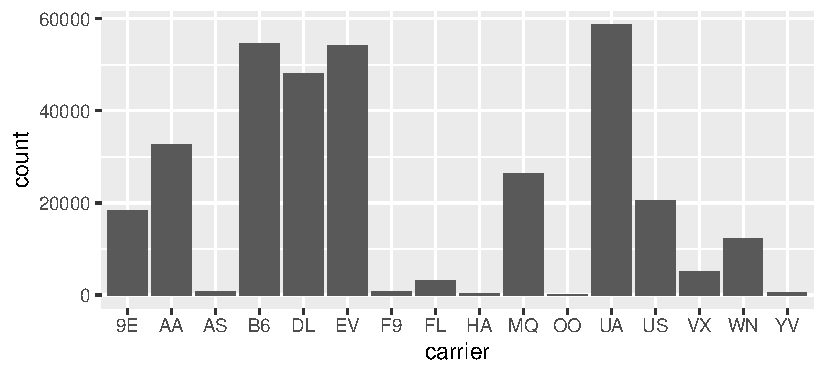
\includegraphics{02-visualization_files/figure-pdf/unnamed-chunk-43-1.pdf}

}

\end{figure}

We can now map the additional variable \texttt{origin} by adding a
\texttt{fill\ =\ origin} inside the \texttt{aes()} aesthetic mapping;
the \texttt{fill} aesthetic of any bar corresponds to the color used to
fill the bars.

\begin{Shaded}
\begin{Highlighting}[]
\FunctionTok{ggplot}\NormalTok{(}\AttributeTok{data =}\NormalTok{ flights, }\AttributeTok{mapping =} \FunctionTok{aes}\NormalTok{(}\AttributeTok{x =}\NormalTok{ carrier, }\AttributeTok{fill =}\NormalTok{ origin)) }\SpecialCharTok{+}
  \FunctionTok{geom\_bar}\NormalTok{()}
\end{Highlighting}
\end{Shaded}

\begin{figure}[H]

{\centering 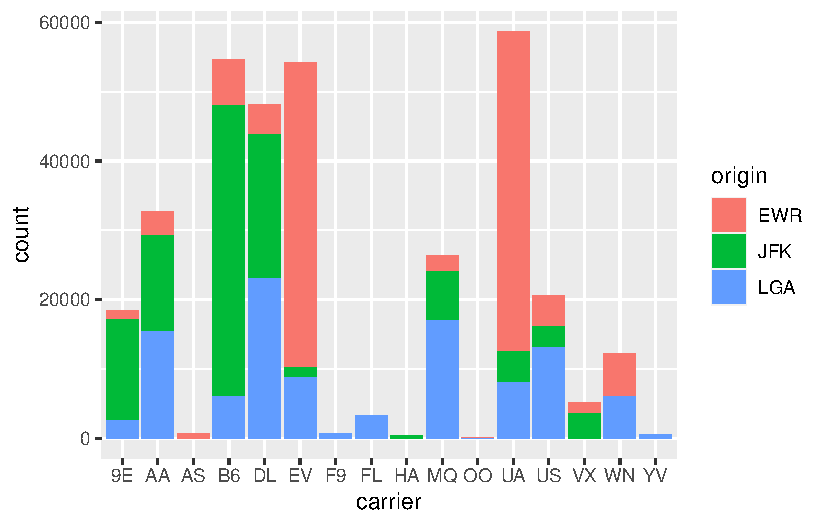
\includegraphics{02-visualization_files/figure-pdf/fig-flights-stacked-bar-1.pdf}

}

\caption{\label{fig-flights-stacked-bar}Stacked barplot comparing the
number of flights by carrier and origin}

\end{figure}

Figure~\ref{fig-flights-stacked-bar} is an example of a \emph{stacked
barplot}. While simple to make, in certain aspects it is not ideal. For
example, it is difficult to compare the heights of the different colors
between the bars, corresponding to comparing the number of flights from
each \texttt{origin} airport between the carriers.

Before we continue, let's address some common points of confusion
amongst new R users. First, note that \texttt{fill} is another aesthetic
mapping much like \texttt{x}-position; thus it must be included within
the parentheses of the \texttt{aes()} mapping. The following code, where
the \texttt{fill} aesthetic is specified outside the \texttt{aes()}
mapping will yield an error. This is a fairly common error that new
\texttt{ggplot} users make:

\begin{Shaded}
\begin{Highlighting}[]
\FunctionTok{ggplot}\NormalTok{(}\AttributeTok{data =}\NormalTok{ flights, }\AttributeTok{mapping =} \FunctionTok{aes}\NormalTok{(}\AttributeTok{x =}\NormalTok{ carrier), }\AttributeTok{fill =}\NormalTok{ origin) }\SpecialCharTok{+}
  \FunctionTok{geom\_bar}\NormalTok{()}
\end{Highlighting}
\end{Shaded}

Second, the \texttt{fill} aesthetic corresponds to the color used to
fill the bars, while the \texttt{color} aesthetic corresponds to the
color of the outline of the bars. Observe in
Figure~\ref{fig-flights-stacked-bar-color} that mapping \texttt{origin}
to \texttt{color} and not \texttt{fill} yields grey bars with different
colored outlines.

\begin{Shaded}
\begin{Highlighting}[]
\FunctionTok{ggplot}\NormalTok{(}\AttributeTok{data =}\NormalTok{ flights, }\AttributeTok{mapping =} \FunctionTok{aes}\NormalTok{(}\AttributeTok{x =}\NormalTok{ carrier, }\AttributeTok{color =}\NormalTok{ origin)) }\SpecialCharTok{+}
  \FunctionTok{geom\_bar}\NormalTok{()}
\end{Highlighting}
\end{Shaded}

\begin{figure}[H]

{\centering 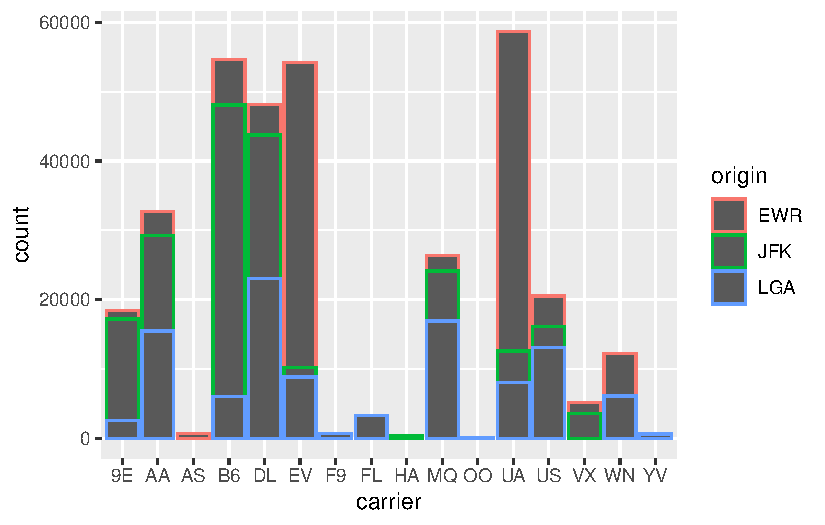
\includegraphics{02-visualization_files/figure-pdf/fig-flights-stacked-bar-color-1.pdf}

}

\caption{\label{fig-flights-stacked-bar-color}Stacked barplot with color
aesthetic used instead of fill}

\end{figure}

\begin{tcolorbox}[enhanced jigsaw, coltitle=black, toprule=.15mm, bottomtitle=1mm, breakable, leftrule=.75mm, title={{🎯} Learning Check 2.32}, opacitybacktitle=0.6, colback=white, rightrule=.15mm, opacityback=0, toptitle=1mm, colbacktitle=quarto-callout-tip-color!10!white, colframe=quarto-callout-tip-color-frame, titlerule=0mm, arc=.35mm, bottomrule=.15mm, left=2mm]
What kinds of questions are not easily answered by looking at the above
figure?
\end{tcolorbox}

\begin{tcolorbox}[enhanced jigsaw, coltitle=black, toprule=.15mm, bottomtitle=1mm, breakable, leftrule=.75mm, title={{🎯} Learning Check 2.33}, opacitybacktitle=0.6, colback=white, rightrule=.15mm, opacityback=0, toptitle=1mm, colbacktitle=quarto-callout-tip-color!10!white, colframe=quarto-callout-tip-color-frame, titlerule=0mm, arc=.35mm, bottomrule=.15mm, left=2mm]
What can you say, if anything, about the relationship between airline
and airport in NYC in 2013 in regards to the number of departing
flights?
\end{tcolorbox}

Another alternative to stacked barplots are \emph{side-by-side
barplots}, also known as a \emph{dodged barplot}. The code to created a
side-by-side barplot is identical to the code to create a stacked
barplot, but with a \texttt{position\ =\ "dodge"} argument added to
\texttt{geom\_bar()}. In other words, we are overriding the default
barplot type, which is a stacked barplot, and specifying it to be a
side-by-side barplot.

\begin{Shaded}
\begin{Highlighting}[]
\FunctionTok{ggplot}\NormalTok{(}\AttributeTok{data =}\NormalTok{ flights, }\AttributeTok{mapping =} \FunctionTok{aes}\NormalTok{(}\AttributeTok{x =}\NormalTok{ carrier, }\AttributeTok{fill =}\NormalTok{ origin)) }\SpecialCharTok{+}
  \FunctionTok{geom\_bar}\NormalTok{(}\AttributeTok{position =} \StringTok{"dodge"}\NormalTok{)}
\end{Highlighting}
\end{Shaded}

\begin{figure}[H]

{\centering 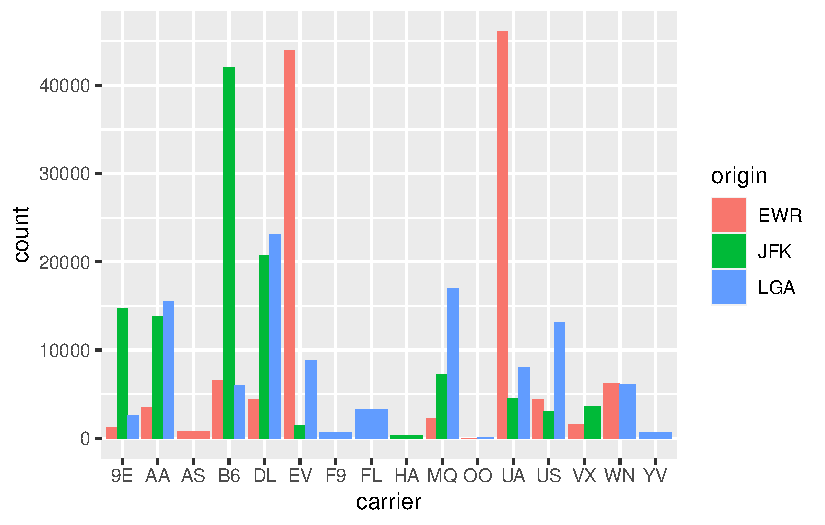
\includegraphics{02-visualization_files/figure-pdf/fig-flights-bar-dodge-1.pdf}

}

\caption{\label{fig-flights-bar-dodge}Side-by-side AKA dodged barplot
comparing the number of flights by carrier and origin}

\end{figure}

\begin{tcolorbox}[enhanced jigsaw, coltitle=black, toprule=.15mm, bottomtitle=1mm, breakable, leftrule=.75mm, title={{🎯} Learning Check 2.34}, opacitybacktitle=0.6, colback=white, rightrule=.15mm, opacityback=0, toptitle=1mm, colbacktitle=quarto-callout-tip-color!10!white, colframe=quarto-callout-tip-color-frame, titlerule=0mm, arc=.35mm, bottomrule=.15mm, left=2mm]
Why might the side-by-side (AKA dodged) barplot be preferable to a
stacked barplot in this case?
\end{tcolorbox}

\begin{tcolorbox}[enhanced jigsaw, coltitle=black, toprule=.15mm, bottomtitle=1mm, breakable, leftrule=.75mm, title={{🎯} Learning Check 2.35}, opacitybacktitle=0.6, colback=white, rightrule=.15mm, opacityback=0, toptitle=1mm, colbacktitle=quarto-callout-tip-color!10!white, colframe=quarto-callout-tip-color-frame, titlerule=0mm, arc=.35mm, bottomrule=.15mm, left=2mm]
What are the disadvantages of using a side-by-side (AKA dodged) barplot,
in general?
\end{tcolorbox}

Lastly, another type of barplot is a \emph{faceted barplot}. Recall in
Section~\ref{sec-facets} we visualized the distribution of hourly
temperatures at the 3 NYC airports \emph{split} by month using facets.
We apply the same principle to our barplot visualizing the frequency of
\texttt{carrier} split by \texttt{origin}: instead of mapping
\texttt{origin}

\begin{Shaded}
\begin{Highlighting}[]
\FunctionTok{ggplot}\NormalTok{(}\AttributeTok{data =}\NormalTok{ flights, }\AttributeTok{mapping =} \FunctionTok{aes}\NormalTok{(}\AttributeTok{x =}\NormalTok{ carrier)) }\SpecialCharTok{+}
  \FunctionTok{geom\_bar}\NormalTok{() }\SpecialCharTok{+}
  \FunctionTok{facet\_wrap}\NormalTok{(}\SpecialCharTok{\textasciitilde{}}\NormalTok{ origin, }\AttributeTok{ncol =} \DecValTok{1}\NormalTok{)}
\end{Highlighting}
\end{Shaded}

\begin{figure}[H]

{\centering \includegraphics{02-visualization_files/figure-pdf/fig-facet-bar-vert-1.pdf}

}

\caption{\label{fig-facet-bar-vert}Faceted barplot comparing the number
of flights by carrier and origin}

\end{figure}

\begin{tcolorbox}[enhanced jigsaw, coltitle=black, toprule=.15mm, bottomtitle=1mm, breakable, leftrule=.75mm, title={{🎯} Learning Check 2.36}, opacitybacktitle=0.6, colback=white, rightrule=.15mm, opacityback=0, toptitle=1mm, colbacktitle=quarto-callout-tip-color!10!white, colframe=quarto-callout-tip-color-frame, titlerule=0mm, arc=.35mm, bottomrule=.15mm, left=2mm]
Why is the faceted barplot preferred to the side-by-side and stacked
barplots in this case?
\end{tcolorbox}

\begin{tcolorbox}[enhanced jigsaw, coltitle=black, toprule=.15mm, bottomtitle=1mm, breakable, leftrule=.75mm, title={{🎯} Learning Check 2.37}, opacitybacktitle=0.6, colback=white, rightrule=.15mm, opacityback=0, toptitle=1mm, colbacktitle=quarto-callout-tip-color!10!white, colframe=quarto-callout-tip-color-frame, titlerule=0mm, arc=.35mm, bottomrule=.15mm, left=2mm]
What information about the different carriers at different airports is
more easily seen in the faceted barplot?
\end{tcolorbox}

\hypertarget{summary-4}{%
\subsection{Summary}\label{summary-4}}

Barplots are the preferred way of displaying the distribution of a
categorical variable, or in other words the frequency with which the
different categories called \emph{levels} occur. They are easy to
understand and make it easy to make comparisons across levels. When
trying to visualize two categorical variables, you have many options:
stacked barplots, side-by-side barplots, and faceted barplots. Depending
on what aspect of the joint distribution you are trying to emphasize,
you will need to make a choice between these three types of barplots.

\hypertarget{sec-data-vis-conclusion}{%
\section{Conclusion}\label{sec-data-vis-conclusion}}

\hypertarget{summary-table}{%
\subsection{Summary table}\label{summary-table}}

Let's recap all five of the Five Named Graphs (5NG) in
Table~\ref{tbl-viz-summary} summarizing their differences. Using these
5NG, you'll be able to visualize the distributions and relationships of
variables contained in a wide array of datasets. This will be even more
the case as we start to map more variables to more of each
\texttt{geom}etric object's \texttt{aes}thetic attribute options,
further unlocking the awesome power of the \texttt{ggplot2} package.

\hypertarget{tbl-viz-summary}{}
\begin{longtable}[]{@{}
  >{\raggedright\arraybackslash}p{(\columnwidth - 6\tabcolsep) * \real{0.0426}}
  >{\raggedright\arraybackslash}p{(\columnwidth - 6\tabcolsep) * \real{0.2730}}
  >{\raggedright\arraybackslash}p{(\columnwidth - 6\tabcolsep) * \real{0.3085}}
  >{\raggedright\arraybackslash}p{(\columnwidth - 6\tabcolsep) * \real{0.3759}}@{}}
\caption{\label{tbl-viz-summary}Summary of 5NG}\tabularnewline
\toprule()
\begin{minipage}[b]{\linewidth}\raggedright
Named graph
\end{minipage} & \begin{minipage}[b]{\linewidth}\raggedright
Shows
\end{minipage} & \begin{minipage}[b]{\linewidth}\raggedright
Geometric object
\end{minipage} & \begin{minipage}[b]{\linewidth}\raggedright
Notes
\end{minipage} \\
\midrule()
\endfirsthead
\toprule()
\begin{minipage}[b]{\linewidth}\raggedright
Named graph
\end{minipage} & \begin{minipage}[b]{\linewidth}\raggedright
Shows
\end{minipage} & \begin{minipage}[b]{\linewidth}\raggedright
Geometric object
\end{minipage} & \begin{minipage}[b]{\linewidth}\raggedright
Notes
\end{minipage} \\
\midrule()
\endhead
Scatterplot & Relationship between 2 numerical variables &
\texttt{geom\_point()} & \\
Linegraph & Relationship between 2 numerical variables &
\texttt{geom\_line()} & Used when there is a sequential order to
x-variable e.g.~time \\
Histogram & Distribution of 1 numerical variable &
\texttt{geom\_histogram()} & Facetted histograms show the distribution
of 1 numerical variable split by the values of another variable \\
Boxplot & Distribution of 1 numerical variable split by the values of
another variable & \texttt{geom\_boxplot()} & \\
Barplot & Distribution of 1 categorical variable & \texttt{geom\_bar()}
when counts are not pre-counted, \texttt{geom\_col()} when counts are
pre-counted & Stacked, side-by-side, and faceted barplots show the joint
distribution of 2 categorical variables \\
\bottomrule()
\end{longtable}

\hypertarget{argument-specification}{%
\subsection{Argument specification}\label{argument-specification}}

Run the following two segments of code. First this:

\begin{Shaded}
\begin{Highlighting}[]
\FunctionTok{ggplot}\NormalTok{(}\AttributeTok{data =}\NormalTok{ flights, }\AttributeTok{mapping =} \FunctionTok{aes}\NormalTok{(}\AttributeTok{x =}\NormalTok{ carrier)) }\SpecialCharTok{+}
  \FunctionTok{geom\_bar}\NormalTok{()}
\end{Highlighting}
\end{Shaded}

then this:

\begin{Shaded}
\begin{Highlighting}[]
\FunctionTok{ggplot}\NormalTok{(flights, }\FunctionTok{aes}\NormalTok{(}\AttributeTok{x =}\NormalTok{ carrier)) }\SpecialCharTok{+}
  \FunctionTok{geom\_bar}\NormalTok{()}
\end{Highlighting}
\end{Shaded}

You'll notice that that both code segments create the same barplot, even
though in the second segment we omitted the \texttt{data\ =} and
\texttt{mapping\ =} code argument names. This is because the
\texttt{ggplot()} by default assumes that the \texttt{data} argument
comes first and the \texttt{mapping} argument comes second. So as long
as you specify the data frame in question first and the \texttt{aes()}
mapping second, you can omit the explicit statement of the argument
names \texttt{data\ =} and \texttt{mapping\ =}.

Going forward for the rest of this book, all \texttt{ggplot()} will be
like the second segment above: with the \texttt{data\ =} and
\texttt{mapping\ =} explicit naming of the argument omitted and the
default ordering of arguments respected.

\hypertarget{additional-resources-1}{%
\subsection{Additional resources}\label{additional-resources-1}}

If you want to further unlock the power of the \texttt{ggplot2} package
for data visualization, we suggest you that you check out RStudio's
``Data Visualization with ggplot2'' cheatsheet. This cheatsheet
summarizes much more than what we've discussed in this chapter, in
particular the many more than the 5 \texttt{geom} geometric objects we
covered in this Chapter, while providing quick and easy to read visual
descriptions.

You can access this cheatsheet by going to the RStudio Menu Bar
-\textgreater{} Help -\textgreater{} Cheatsheets -\textgreater{} ``Data
Visualization with ggplot2'':

\begin{figure}

{\centering \includegraphics{images/ggplot_cheatsheet-1.png}

}

\caption{\label{fig-ggplot-cheatsheet}Data Visualization with ggplot2
cheatsheat}

\end{figure}

\hypertarget{sec-whats-to-come-3}{%
\subsection{What's to come}\label{sec-whats-to-come-3}}

Recall in Figure~\ref{fig-noalpha} in Section~\ref{sec-scatterplots} we
visualized the relationship between departure delay and arrival delay
for Alaska Airlines flights. This necessitated paring or filtering down
the \texttt{flights} data frame to a new data frame
\texttt{alaska\_flights} consisting of only \texttt{carrier\ ==\ AS}
flights first:

\begin{Shaded}
\begin{Highlighting}[]
\NormalTok{alaska\_flights }\OtherTok{\textless{}{-}}\NormalTok{ flights }\SpecialCharTok{\%\textgreater{}\%} 
  \FunctionTok{filter}\NormalTok{(carrier }\SpecialCharTok{==} \StringTok{"AS"}\NormalTok{)}

\FunctionTok{ggplot}\NormalTok{(}\AttributeTok{data =}\NormalTok{ alaska\_flights, }\AttributeTok{mapping =} \FunctionTok{aes}\NormalTok{(}\AttributeTok{x =}\NormalTok{ dep\_delay, }\AttributeTok{y =}\NormalTok{ arr\_delay)) }\SpecialCharTok{+} 
  \FunctionTok{geom\_point}\NormalTok{()}
\end{Highlighting}
\end{Shaded}

Furthermore recall in Figure~\ref{fig-hourlytemp} in
Section~\ref{sec-linegraphs} we visualized hourly temperature recordings
at Newark airport only for the first 15 days of January 2013. This
necessitated paring or fitlering down the \texttt{weather} data frame to
a new data frame \texttt{early\_january\_weather} consisting of hourly
temperature recordings only for \texttt{origin\ ==\ "EWR"},
\texttt{month\ ==\ 1}, and day less than or equal to \texttt{15} first:

\begin{Shaded}
\begin{Highlighting}[]
\NormalTok{early\_january\_weather }\OtherTok{\textless{}{-}}\NormalTok{ weather }\SpecialCharTok{\%\textgreater{}\%} 
  \FunctionTok{filter}\NormalTok{(origin }\SpecialCharTok{==} \StringTok{"EWR"} \SpecialCharTok{\&}\NormalTok{ month }\SpecialCharTok{==} \DecValTok{1} \SpecialCharTok{\&}\NormalTok{ day }\SpecialCharTok{\textless{}=} \DecValTok{15}\NormalTok{)}

\FunctionTok{ggplot}\NormalTok{(}\AttributeTok{data =}\NormalTok{ early\_january\_weather, }\AttributeTok{mapping =} \FunctionTok{aes}\NormalTok{(}\AttributeTok{x =}\NormalTok{ time\_hour, }\AttributeTok{y =}\NormalTok{ temp)) }\SpecialCharTok{+}
  \FunctionTok{geom\_line}\NormalTok{()}
\end{Highlighting}
\end{Shaded}

These two code segments were a preview of Chapter~\ref{sec-wrangling} on
data wrangling where we'll delve further into the \texttt{dplyr}
package. Data wrangling is the process of transforming and modifying
existing data with the intent of making it more appropriate for analysis
purposes. For example, the two code segments used the \texttt{filter()}
function to create new data frames (\texttt{alaska\_flights} and
\texttt{early\_january\_weather}) by choosing only a subset of rows of
existing data frames (\texttt{flights} and \texttt{weather}). In this
next chapter, we'll formally introduce the \texttt{filter()} and other
data wrangling functions as well as the \emph{pipe operator}
\texttt{\%\textgreater{}\%} which allows you to combine multiple data
wrangling actions into a single sequential \emph{chain} of actions. On
to Chapter~\ref{sec-wrangling} on data wrangling!

\hypertarget{sec-ex02}{%
\section{Exercises}\label{sec-ex02}}

\hypertarget{sec-ex02-conceptual}{%
\subsection{Conceptual}\label{sec-ex02-conceptual}}

\leavevmode\vadjust pre{\hypertarget{exr-ch02-c01}{}}%
\begin{exercise}[]\label{exr-ch02-c01}

Which of the following layers could be added to create one of the five
named graphs (5NG)? Select all that apply.

\begin{enumerate}
\def\labelenumi{\alph{enumi})}
\tightlist
\item
  \texttt{geom\_smooth()}
\item
  \texttt{geom\_line()}
\item
  \texttt{geom\_col()}
\item
  \texttt{geom\_box()}
\item
  \texttt{geom\_histogram()}
\item
  \texttt{facet\_wrap()}
\end{enumerate}

\end{exercise}

\leavevmode\vadjust pre{\hypertarget{exr-ch02-c02}{}}%
\begin{exercise}[]\label{exr-ch02-c02}

What layer is add to create a scatterplot?

\begin{enumerate}
\def\labelenumi{\alph{enumi})}
\tightlist
\item
  \texttt{geom\_line()}
\item
  \texttt{geom\_scatter()}
\item
  \texttt{geom\_jitter()}
\item
  \texttt{geom\_point()}
\item
  none of the above
\end{enumerate}

\end{exercise}

\leavevmode\vadjust pre{\hypertarget{exr-ch02-c03}{}}%
\begin{exercise}[]\label{exr-ch02-c03}

Which of the following options are solutions to overplotting? Select all
that apply.

\begin{enumerate}
\def\labelenumi{\alph{enumi})}
\tightlist
\item
  Changing the x and y variables
\item
  Changing the transparency
\item
  Changing the limits of the x and y axes
\item
  Plotting only some of the data
\item
  Jittering the points
\end{enumerate}

\end{exercise}

\leavevmode\vadjust pre{\hypertarget{exr-ch02-c04}{}}%
\begin{exercise}[]\label{exr-ch02-c04}

When is it useful to facet your data?

\begin{enumerate}
\def\labelenumi{\alph{enumi})}
\tightlist
\item
  When you want to see the shape of the entire distribution without
  separation
\item
  When you want to split a particular visualization of variables by
  another variable
\item
  When you are interested in looking at how your plot differs by year
  when year is a continuous variable
\item
  When you think your variables have incorrect data in them
\item
  When you have lots of missing values
\end{enumerate}

\end{exercise}

\leavevmode\vadjust pre{\hypertarget{exr-ch02-c05}{}}%
\begin{exercise}[]\label{exr-ch02-c05}

Consider the following dataset which counts the total number of career
wins for three NBA players. Which layer is added to visualize the
distribution of the number of wins each \texttt{player} had over their
career?

\begin{longtable}[]{@{}ll@{}}
\toprule()
player & num\_wins \\
\midrule()
\endhead
Kobe Bryant & 1057 \\
LeBron James & 1089 \\
Michael Jordan & 829 \\
\bottomrule()
\end{longtable}

\begin{enumerate}
\def\labelenumi{\alph{enumi})}
\tightlist
\item
  \texttt{geom\_bar()}
\item
  \texttt{geom\_col()}
\item
  all of the above
\item
  none of the above
\end{enumerate}

\end{exercise}

\leavevmode\vadjust pre{\hypertarget{exr-ch02-c06}{}}%
\begin{exercise}[]\label{exr-ch02-c06}

Which of the following graphs would be \textbf{MOST} useful for
comparing the distribution of weights for different species of cats?

\begin{enumerate}
\def\labelenumi{\alph{enumi})}
\tightlist
\item
  grouped boxplot
\item
  histogram
\item
  stacked barplot
\item
  scatterplot
\item
  faceted barplot
\end{enumerate}

\end{exercise}

\leavevmode\vadjust pre{\hypertarget{exr-ch02-c07}{}}%
\begin{exercise}[]\label{exr-ch02-c07}

Which of the following graphs would be \textbf{MOST} useful for
visualizing the daily weather temperatures in January for Chicago?

\begin{enumerate}
\def\labelenumi{\alph{enumi})}
\tightlist
\item
  scatterplot
\item
  linegraph
\item
  histogram
\item
  faceted scatterplot
\item
  grouped boxplot
\end{enumerate}

\end{exercise}

\leavevmode\vadjust pre{\hypertarget{exr-ch02-c08}{}}%
\begin{exercise}[]\label{exr-ch02-c08}

Which of the following graphs would be \textbf{MOST} useful for
visualizing the relationship between bank account balances and annual
incomes?

\begin{enumerate}
\def\labelenumi{\alph{enumi})}
\tightlist
\item
  faceted histogram
\item
  linegraph
\item
  scatterplot
\item
  stacked barplot
\item
  boxplot
\end{enumerate}

\end{exercise}

\leavevmode\vadjust pre{\hypertarget{exr-ch02-c09}{}}%
\begin{exercise}[]\label{exr-ch02-c09}

Which of the following graphs would be \textbf{MOST} useful for finding
outliers?

\begin{enumerate}
\def\labelenumi{\alph{enumi})}
\tightlist
\item
  scatterplot
\item
  linegraph
\item
  histogram
\item
  boxplot
\item
  barplot
\end{enumerate}

\end{exercise}

\leavevmode\vadjust pre{\hypertarget{exr-ch02-c10}{}}%
\begin{exercise}[]\label{exr-ch02-c10}

Below is a scatterplot of a fictional dataset depicting the amount of
money spent in a grocery store by the amount of time in the store.
Describe the relationship.

\includegraphics[width=\textwidth,height=2in]{images/exercises/ch02_scatter.png}

\end{exercise}

\leavevmode\vadjust pre{\hypertarget{exr-ch02-c11}{}}%
\begin{exercise}[]\label{exr-ch02-c11}

Describe the modality and skew of the histogram below.

\includegraphics[width=\textwidth,height=2in]{images/exercises/ch02_match_hist.png}

\end{exercise}

\leavevmode\vadjust pre{\hypertarget{exr-ch02-c12}{}}%
\begin{exercise}[]\label{exr-ch02-c12}

Match the histogram with the corresponding boxplot.

\includegraphics[width=\textwidth,height=2in]{images/exercises/ch02_match_hist.png}
\includegraphics[width=\textwidth,height=2in]{images/exercises/ch02_match_box.png}

\end{exercise}

\hypertarget{sec-ex02-application}{%
\subsection{Application}\label{sec-ex02-application}}

Use the \texttt{covid\_sub} dataset created below for the following
problem. The dataset is derived from the \texttt{covid\_states} dataset
in the \texttt{ISDSdatasets} package.

\begin{Shaded}
\begin{Highlighting}[]
\NormalTok{covid\_sub }\OtherTok{\textless{}{-}}\NormalTok{ covid\_states }\SpecialCharTok{\%\textgreater{}\%} 
  \FunctionTok{filter}\NormalTok{(}
\NormalTok{    state\_abbr }\SpecialCharTok{==} \StringTok{"IL"} \SpecialCharTok{|}\NormalTok{ state\_abbr }\SpecialCharTok{==} \StringTok{"FL"}\NormalTok{,}
\NormalTok{    date }\SpecialCharTok{\textgreater{}=} \StringTok{"2021{-}07{-}01"}\NormalTok{, date }\SpecialCharTok{\textless{}=} \StringTok{"2021{-}08{-}31"}\NormalTok{,}
\NormalTok{    wday }\SpecialCharTok{!=} \StringTok{"Sat"}\NormalTok{, wday }\SpecialCharTok{!=} \StringTok{"Sun"}
\NormalTok{    )}
\end{Highlighting}
\end{Shaded}

You will learn about data wrangling in the next Chapter. The code reads
as follows: take the dataset \texttt{covid\_states} and then subset the
data to only include observations in the states \texttt{"IL"} or
\texttt{"FL"}, and only include observations between July 1, 2021 and
August 31, 2021 (inclusive), and only observations not recorded on
Saturday, and observations not recorded on Sunday. Note: COVID reporting
was not done on weekends or holidays in these states.

\leavevmode\vadjust pre{\hypertarget{exr-ch02-app1}{}}%
\begin{exercise}[]\label{exr-ch02-app1}

Plot a linegraph of the number of new COVID cases from July to August
2021 for Illinois and Florida. Use the \texttt{color} aesthetic to have
separate lines for each state. Compare and describe the linegraph.

\end{exercise}

\begin{center}\rule{0.5\linewidth}{0.5pt}\end{center}

Use the \texttt{nba} dataset in the \texttt{ISDSdatasets} package for
exercises Exercise~\ref{exr-ch02-app2}, Exercise~\ref{exr-ch02-app3},
and Exercise~\ref{exr-ch02-app4}.

\leavevmode\vadjust pre{\hypertarget{exr-ch02-app2}{}}%
\begin{exercise}[]\label{exr-ch02-app2}

Describe and compare the number of wins and losses faceted by player
using a barplot.

\end{exercise}

\leavevmode\vadjust pre{\hypertarget{exr-ch02-app3}{}}%
\begin{exercise}[]\label{exr-ch02-app3}

Plot and describe the relationship between field goal percentage
(\texttt{fg\_percent}) and free throw percentage (\texttt{ft\_percent}).
Adjust for overplotting if need be.

\end{exercise}

\leavevmode\vadjust pre{\hypertarget{exr-ch02-app4}{}}%
\begin{exercise}[]\label{exr-ch02-app4}

Compare the center, spread, and shape of the distribution of
\texttt{pts} scored per game by \texttt{player} for regular season games
and playoff games. In other words, facet the plot of \texttt{pts} by
\texttt{player} based on \texttt{season}.

\end{exercise}

\hypertarget{sec-ex02-advanced}{%
\subsection{Advanced}\label{sec-ex02-advanced}}

Let's learn some advanced plotting features.

\leavevmode\vadjust pre{\hypertarget{exr-ch02-adv1}{}}%
\begin{exercise}[]\label{exr-ch02-adv1}

Start with your plot from Exercise~\ref{exr-ch02-app1}. Let's clean up
the graph a little by adding the following layers:

\begin{enumerate}
\def\labelenumi{\alph{enumi})}
\tightlist
\item
  add on \texttt{theme\_minimal()}
\item
  remove the x-axis label by setting \texttt{x\ =\ NULL} in the
  \texttt{labs()}
\item
  To make the x-axis text easier to read we will rotate it 45 degrees
  and horizontally align it on the right. Add the layer
  \texttt{theme(axis.text.x\ =\ element\_text(angle\ =\ ?,\ hjust\ =\ ?))}
  but replace the ? with the appropriate values.
\end{enumerate}

\end{exercise}

\leavevmode\vadjust pre{\hypertarget{exr-ch02-adv2}{}}%
\begin{exercise}[]\label{exr-ch02-adv2}

Use the \texttt{nba\_pct} dataset created below to plot the average free
throw percent for each player.

\begin{Shaded}
\begin{Highlighting}[]
\NormalTok{nba\_pct }\OtherTok{\textless{}{-}}\NormalTok{ nba }\SpecialCharTok{\%\textgreater{}\%} 
    \FunctionTok{group\_by}\NormalTok{(player) }\SpecialCharTok{\%\textgreater{}\%}
    \FunctionTok{summarize}\NormalTok{(}\AttributeTok{avg\_ft\_pct =} \FunctionTok{mean}\NormalTok{(ft\_percent, }\AttributeTok{na.rm =} \ConstantTok{TRUE}\NormalTok{))}
\end{Highlighting}
\end{Shaded}

\begin{enumerate}
\def\labelenumi{\alph{enumi})}
\tightlist
\item
  Change the y-axis label to percents by adding the following layer
  \texttt{scale\_y\_*(labels\ =\ scales::percent)}. Replace the * with
  the data type. May be useful to check the help documentation.
\item
  Reorder the x-axis from highest to lowest with the following layer:
  \texttt{scale\_x\_*(limits\ =\ c("Kobe\ Bryant",\ "Michael\ Jordan",\ "LeBron\ James"))}.
  Again replace the * with the appropriate data type.
\end{enumerate}

\end{exercise}

\hypertarget{sec-wrangling}{%
\chapter{Data Wrangling}\label{sec-wrangling}}

So far in our journey, we've seen how to look at data saved in data
frames using the \texttt{glimpse()} and \texttt{View()} functions in
Chapter~\ref{sec-getting-started} on and how to create data
visualizations using the \texttt{ggplot2} package in
Chapter~\ref{sec-viz}. In particular we studied what we term the ``five
named graphs'' (5NG):

\begin{enumerate}
\def\labelenumi{\arabic{enumi}.}
\tightlist
\item
  scatterplots via \texttt{geom\_point()}
\item
  linegraphs via \texttt{geom\_line()}
\item
  boxplots via \texttt{geom\_boxplot()}
\item
  histograms via \texttt{geom\_histogram()}
\item
  barplots via \texttt{geom\_bar()} or \texttt{geom\_col()}
\end{enumerate}

We created these visualizations using the ``Grammar of Graphics'', which
maps variables in a data frame to the aesthetic attributes of one the
above 5 \texttt{geom}etric objects. We can also control other aesthetic
attributes of the geometric objects such as the size and color as seen
in the Gapminder data example in Figure~\ref{fig-gapminder}.

Recall however in Section~\ref{sec-whats-to-come-3} we discussed that
for two of our visualizations we needed transformed/modified versions of
existing data frames. Recall for example the scatterplot of departure
and arrival delay \emph{only} for Alaska Airlines flights. In order to
create this visualization, we needed to first pare down the
\texttt{flights} data frame to a new data frame \texttt{alaska\_flights}
consisting of only \texttt{carrier\ ==\ "AS"} flights using the
\texttt{filter()} function.

\begin{Shaded}
\begin{Highlighting}[]
\NormalTok{alaska\_flights }\OtherTok{\textless{}{-}}\NormalTok{ flights }\SpecialCharTok{\%\textgreater{}\%} 
  \FunctionTok{filter}\NormalTok{(carrier }\SpecialCharTok{==} \StringTok{"AS"}\NormalTok{)}

\FunctionTok{ggplot}\NormalTok{(}\AttributeTok{data =}\NormalTok{ alaska\_flights, }\AttributeTok{mapping =} \FunctionTok{aes}\NormalTok{(}\AttributeTok{x =}\NormalTok{ dep\_delay, }\AttributeTok{y =}\NormalTok{ arr\_delay)) }\SpecialCharTok{+} 
  \FunctionTok{geom\_point}\NormalTok{()}
\end{Highlighting}
\end{Shaded}

In this chapter, we'll introduce a series of functions from the
\texttt{dplyr} package that will allow you to take a data frame and

\begin{enumerate}
\def\labelenumi{\arabic{enumi}.}
\item
  \texttt{filter()} its existing rows to only pick out a subset of them.
  For example, the \texttt{alaska\_flights} data frame above.
\item
  \texttt{summarize()} one of its columns/variables with a \emph{summary
  statistic}. Examples include the median and interquartile range of
  temperatures as we saw in Section~\ref{sec-boxplots} on boxplots.
\item
  \texttt{group\_by()} its rows. In other words assign different rows to
  be part of the same \emph{group} and report summary statistics for
  each group separately. For example, say perhaps you don't want a
  single overall average departure delay \texttt{dep\_delay} for all
  three \texttt{origin} airports combined, but rather three separate
  average departure delays, one for each of the three \texttt{origin}
  airports.
\item
  \texttt{mutate()} its existing columns/variables to create new ones.
  For example, convert hourly temperature recordings from °F to °C.
\item
  \texttt{arrange()} its rows. For example, sort the rows of
  \texttt{weather} in ascending or descending order of \texttt{temp}.
\item
  \texttt{join()} it with another data frame by matching along a ``key''
  variable. In other words, merge these two data frames together.
\end{enumerate}

Notice how we used \texttt{computer\ code} font to describe the actions
we want to take on our data frames. This is because the \texttt{dplyr}
package for data wrangling that we'll introduce in this chapter has
intuitively verb-named functions that are easy to remember.

We'll start by introducing the pipe operator
\texttt{\%\textgreater{}\%}, which allows you to combine multiple data
wrangling verb-named functions into a single sequential \emph{chain} of
actions.

\hypertarget{packages-needed-1}{%
\section*{Packages Needed}\label{packages-needed-1}}
\addcontentsline{toc}{section}{Packages Needed}

Let's load all the packages needed for this chapter (this assumes you've
already installed them). If needed, read Section~\ref{sec-packages} for
information on how to install and load R packages.

\begin{Shaded}
\begin{Highlighting}[]
\FunctionTok{library}\NormalTok{(dplyr)}
\FunctionTok{library}\NormalTok{(ggplot2)}
\FunctionTok{library}\NormalTok{(nycflights13)}
\end{Highlighting}
\end{Shaded}

\hypertarget{sec-piping}{%
\section{\texorpdfstring{The pipe operator:
\texttt{\%\textgreater{}\%}}{The pipe operator: \%\textgreater\%}}\label{sec-piping}}

Before we start data wrangling, let's first introduce a very nifty tool
that gets loaded along with the \texttt{dplyr} package: the pipe
operator \texttt{\%\textgreater{}\%}. Say you would like to perform a
hypothetical sequence of operations on a hypothetical data frame
\texttt{x} using hypothetical functions \texttt{f()}, \texttt{g()}, and
\texttt{h()}:

\begin{enumerate}
\def\labelenumi{\arabic{enumi}.}
\tightlist
\item
  Take \texttt{x} \emph{then}
\item
  Use \texttt{x} as an input to a function \texttt{f()} \emph{then}
\item
  Use the output of \texttt{f(x)} as an input to a function \texttt{g()}
  \emph{then}
\item
  Use the output of \texttt{g(f(x))} as an input to a function
  \texttt{h()}
\end{enumerate}

One way to achieve this sequence of operations is by using nesting
parentheses as follows:

\begin{Shaded}
\begin{Highlighting}[]
\FunctionTok{h}\NormalTok{(}\FunctionTok{g}\NormalTok{(}\FunctionTok{f}\NormalTok{(x)))}
\end{Highlighting}
\end{Shaded}

The above code isn't so hard to read since we are applying only three
functions: \texttt{f()}, then \texttt{g()}, then \texttt{h()}. However,
you can imagine that this can get progressively harder and harder to
read as the number of functions applied in your sequence increases. This
is where the pipe operator \texttt{\%\textgreater{}\%} comes in handy.
\texttt{\%\textgreater{}\%} takes one output of one function and then
``pipes'' it to be the input of the next function. Furthermore, a
helpful trick is to read \texttt{\%\textgreater{}\%} as ``then.'' For
example, you can obtain the same output as the above sequence of
operations as follows:

\begin{Shaded}
\begin{Highlighting}[]
\NormalTok{x }\SpecialCharTok{\%\textgreater{}\%} 
  \FunctionTok{f}\NormalTok{() }\SpecialCharTok{\%\textgreater{}\%} 
  \FunctionTok{g}\NormalTok{() }\SpecialCharTok{\%\textgreater{}\%} 
  \FunctionTok{h}\NormalTok{()}
\end{Highlighting}
\end{Shaded}

You would read this above sequence as:

\begin{enumerate}
\def\labelenumi{\arabic{enumi}.}
\tightlist
\item
  Take \texttt{x} \emph{then}
\item
  Use this output as the input to the next function \texttt{f()}
  \emph{then}
\item
  Use this output as the input to the next function \texttt{g()}
  \emph{then}
\item
  Use this output as the input to the next function \texttt{h()}
\end{enumerate}

So while both approaches above would achieve the same goal, the latter
is much more human-readable because you can read the sequence of
operations line-by-line. But what are the hypothetical \texttt{x},
\texttt{f()}, \texttt{g()}, and \texttt{h()}? Throughout this chapter on
data wrangling:

\begin{itemize}
\item
  The starting value \texttt{x} will be a data frame. For example:
  \texttt{flights}.
\item
  The sequence of functions, here \texttt{f()}, \texttt{g()}, and
  \texttt{h()}, will be a sequence of any number of the 6 data wrangling
  verb-named functions we listed in the introduction to this chapter.
  For example: \texttt{filter(carrier\ ==\ "AS")}.
\item
  The result will be the transformed/modified data frame that you want.
  For example: a data frame consisting of only the subset of rows in
  \texttt{flights} corresponding to Alaska Airlines flights.
\end{itemize}

Much like when adding layers to a \texttt{ggplot()} using the \texttt{+}
sign at the end of lines, you form a single \emph{chain} of data
wrangling operations by combining verb-named functions into a single
sequence with pipe operators \texttt{\%\textgreater{}\%} at the end of
lines. So continuing our example involving Alaska Airlines flights, we
form a chain using the pipe operator \texttt{\%\textgreater{}\%} and
save the resulting data frame in \texttt{alaska\_flights}:

\begin{Shaded}
\begin{Highlighting}[]
\NormalTok{alaska\_flights }\OtherTok{\textless{}{-}}\NormalTok{ flights }\SpecialCharTok{\%\textgreater{}\%} 
  \FunctionTok{filter}\NormalTok{(carrier }\SpecialCharTok{==} \StringTok{"AS"}\NormalTok{)}
\end{Highlighting}
\end{Shaded}

Keep in mind, there are many more advanced data wrangling functions than
just the 6 listed in the introduction to this chapter; you'll see some
examples of these in Section~\ref{sec-other-verbs}. However, just with
these 6 verb-named functions you'll be able to perform a broad array of
data wrangling tasks for the rest of this book.

\hypertarget{sec-filter}{%
\section{\texorpdfstring{\texttt{filter()}
rows}{filter() rows}}\label{sec-filter}}

\begin{figure}

{\centering \includegraphics{images/filter.png}

}

\caption{\label{fig-filter}Diagram of filter()}

\end{figure}

The \texttt{filter()} function here works much like the ``Filter''
option in Microsoft Excel; it allows you to specify criteria about the
values of a variable in your dataset and then filters out only those
rows that match that criteria. We begin by focusing only on flights from
New York City to Portland, Oregon. The \texttt{dest} code (or airport
code) for Portland, Oregon is \texttt{"PDX"}. Run the following and look
at the resulting spreadsheet to ensure that only flights heading to
Portland are chosen here:

\begin{Shaded}
\begin{Highlighting}[]
\NormalTok{portland\_flights }\OtherTok{\textless{}{-}}\NormalTok{ flights }\SpecialCharTok{\%\textgreater{}\%} 
  \FunctionTok{filter}\NormalTok{(dest }\SpecialCharTok{==} \StringTok{"PDX"}\NormalTok{)}

\FunctionTok{View}\NormalTok{(portland\_flights)}
\end{Highlighting}
\end{Shaded}

Note the following:

\begin{itemize}
\tightlist
\item
  The ordering of the commands:

  \begin{itemize}
  \tightlist
  \item
    Take the \texttt{flights} data frame \texttt{flights} \emph{then}
  \item
    \texttt{filter} the data frame so that only those where the
    \texttt{dest} equals \texttt{"PDX"} are included.
  \end{itemize}
\item
  We test for equality using the double equal sign \texttt{==} and not a
  single equal sign \texttt{=}. In other words
  \texttt{filter(dest\ =\ "PDX")} will yield an error. This is a
  convention across many programming languages. If you are new to
  coding, you'll probably forget to use the double equal sign
  \texttt{==} a few times before you get the hang of it.
\end{itemize}

You can use other mathematical operations beyond just \texttt{==} to
form criteria:

\begin{itemize}
\tightlist
\item
  \texttt{\textgreater{}} corresponds to ``greater than''
\item
  \texttt{\textless{}} corresponds to ``less than''
\item
  \texttt{\textgreater{}=} corresponds to ``greater than or equal to''
\item
  \texttt{\textless{}=} corresponds to ``less than or equal to''
\item
  \texttt{!=} corresponds to ``not equal to''. The \texttt{!} is used in
  many programming languages to indicate ``not''.
\end{itemize}

Furthermore, you can combine multiple criteria together using operators
that make comparisons:

\begin{itemize}
\tightlist
\item
  \texttt{\textbar{}} corresponds to ``or''
\item
  \texttt{\&} corresponds to ``and''
\end{itemize}

To see many of these in action, let's filter \texttt{flights} for all
rows that:

\begin{itemize}
\tightlist
\item
  Departed from JFK airport and
\item
  Were heading to Burlington, Vermont (\texttt{"BTV"}) or Seattle,
  Washington (\texttt{"SEA"}) and
\item
  Departed in the months of October, November, or December.
\end{itemize}

Run the following:

\begin{Shaded}
\begin{Highlighting}[]
\NormalTok{btv\_sea\_flights\_fall }\OtherTok{\textless{}{-}}\NormalTok{ flights }\SpecialCharTok{\%\textgreater{}\%} 
  \FunctionTok{filter}\NormalTok{(origin }\SpecialCharTok{==} \StringTok{"JFK"} \SpecialCharTok{\&}\NormalTok{ (dest }\SpecialCharTok{==} \StringTok{"BTV"} \SpecialCharTok{|}\NormalTok{ dest }\SpecialCharTok{==} \StringTok{"SEA"}\NormalTok{) }\SpecialCharTok{\&}\NormalTok{ month }\SpecialCharTok{\textgreater{}=} \DecValTok{10}\NormalTok{)}

\FunctionTok{View}\NormalTok{(btv\_sea\_flights\_fall)}
\end{Highlighting}
\end{Shaded}

Note that even though colloquially speaking one might say ``all flights
leaving Burlington, Vermont \emph{and} Seattle, Washington,'' in terms
of computer operations, we really mean ``all flights leaving Burlington,
Vermont \emph{or} leaving Seattle, Washington.'' For a given row in the
data, \texttt{dest} can be ``BTV'', ``SEA'', or something else, but not
``BTV'' and ``SEA'' at the same time. Furthermore, note the careful use
of parentheses around the
\texttt{dest\ ==\ "BTV"\ \textbar{}\ dest\ ==\ "SEA"}.

We can often skip the use of \texttt{\&} and just separate our
conditions with a comma. In other words the code above will return the
identical output \texttt{btv\_sea\_flights\_fall} as this code below:

\begin{Shaded}
\begin{Highlighting}[]
\NormalTok{btv\_sea\_flights\_fall }\OtherTok{\textless{}{-}}\NormalTok{ flights }\SpecialCharTok{\%\textgreater{}\%} 
  \FunctionTok{filter}\NormalTok{(origin }\SpecialCharTok{==} \StringTok{"JFK"}\NormalTok{, (dest }\SpecialCharTok{==} \StringTok{"BTV"} \SpecialCharTok{|}\NormalTok{ dest }\SpecialCharTok{==} \StringTok{"SEA"}\NormalTok{), month }\SpecialCharTok{\textgreater{}=} \DecValTok{10}\NormalTok{)}

\FunctionTok{View}\NormalTok{(btv\_sea\_flights\_fall)}
\end{Highlighting}
\end{Shaded}

Let's present another example that uses the \texttt{!} ``not'' operator
to pick rows that \emph{don't} match a criteria. As mentioned earlier,
the \texttt{!} can be read as ``not.'' Here we are filtering rows
corresponding to flights that didn't go to Burlington, VT or Seattle,
WA.

\begin{Shaded}
\begin{Highlighting}[]
\NormalTok{not\_BTV\_SEA }\OtherTok{\textless{}{-}}\NormalTok{ flights }\SpecialCharTok{\%\textgreater{}\%} 
  \FunctionTok{filter}\NormalTok{(}\SpecialCharTok{!}\NormalTok{(dest }\SpecialCharTok{==} \StringTok{"BTV"} \SpecialCharTok{|}\NormalTok{ dest }\SpecialCharTok{==} \StringTok{"SEA"}\NormalTok{))}

\FunctionTok{View}\NormalTok{(not\_BTV\_SEA)}
\end{Highlighting}
\end{Shaded}

Again, note the careful use of parentheses around the
\texttt{(dest\ ==\ "BTV"\ \textbar{}\ dest\ ==\ "SEA")}. If we didn't
use parentheses as follows:

\begin{Shaded}
\begin{Highlighting}[]
\NormalTok{flights }\SpecialCharTok{\%\textgreater{}\%} 
  \FunctionTok{filter}\NormalTok{(}\SpecialCharTok{!}\NormalTok{dest }\SpecialCharTok{==} \StringTok{"BTV"} \SpecialCharTok{|}\NormalTok{ dest }\SpecialCharTok{==} \StringTok{"SEA"}\NormalTok{)}
\end{Highlighting}
\end{Shaded}

We would be returning all flights not headed to \texttt{"BTV"} \emph{or}
those headed to \texttt{"SEA"}, which is an entirely different resulting
data frame.

Now say we have a large list of airports we want to filter for, say
\texttt{BTV}, \texttt{SEA}, \texttt{PDX}, \texttt{SFO}, and
\texttt{BDL}. We could continue to use the \texttt{\textbar{}} or
operator as so:

\begin{Shaded}
\begin{Highlighting}[]
\NormalTok{many\_airports }\OtherTok{\textless{}{-}}\NormalTok{ flights }\SpecialCharTok{\%\textgreater{}\%} 
  \FunctionTok{filter}\NormalTok{(dest }\SpecialCharTok{==} \StringTok{"BTV"} \SpecialCharTok{|}\NormalTok{ dest }\SpecialCharTok{==} \StringTok{"SEA"} \SpecialCharTok{|}\NormalTok{ dest }\SpecialCharTok{==} \StringTok{"PDX"} \SpecialCharTok{|}\NormalTok{ dest }\SpecialCharTok{==} \StringTok{"SFO"} \SpecialCharTok{|}\NormalTok{ dest }\SpecialCharTok{==} \StringTok{"BDL"}\NormalTok{)}

\FunctionTok{View}\NormalTok{(many\_airports)}
\end{Highlighting}
\end{Shaded}

but as we progressively include more airports, this will get unwieldy. A
slightly shorter approach uses the \texttt{\%in\%} operator:

\begin{Shaded}
\begin{Highlighting}[]
\NormalTok{many\_airports }\OtherTok{\textless{}{-}}\NormalTok{ flights }\SpecialCharTok{\%\textgreater{}\%} 
  \FunctionTok{filter}\NormalTok{(dest }\SpecialCharTok{\%in\%} \FunctionTok{c}\NormalTok{(}\StringTok{"BTV"}\NormalTok{, }\StringTok{"SEA"}\NormalTok{, }\StringTok{"PDX"}\NormalTok{, }\StringTok{"SFO"}\NormalTok{, }\StringTok{"BDL"}\NormalTok{))}

\FunctionTok{View}\NormalTok{(many\_airports)}
\end{Highlighting}
\end{Shaded}

What this code is doing is filtering \texttt{flights} for all flights
where \texttt{dest} is in the list of airports
\texttt{c("BTV",\ "SEA",\ "PDX",\ "SFO",\ "BDL")}. Recall from
Chapter~\ref{sec-getting-started} that the \texttt{c()} function
``combines'' or ``concatenates'' values in a vector of values. Both
outputs of \texttt{many\_airports} are the same, but as you can see the
latter takes much less time to code.

As a final note we point out that \texttt{filter()} should often be
among the first verbs you apply to your data. This cleans your dataset
to only those rows you care about, or put differently, it narrows down
the scope of your data frame to just the observations your care about.

\begin{tcolorbox}[enhanced jigsaw, coltitle=black, toprule=.15mm, bottomtitle=1mm, breakable, leftrule=.75mm, title={{🎯} Learning Check 3.1}, opacitybacktitle=0.6, colback=white, rightrule=.15mm, opacityback=0, toptitle=1mm, colbacktitle=quarto-callout-tip-color!10!white, colframe=quarto-callout-tip-color-frame, titlerule=0mm, arc=.35mm, bottomrule=.15mm, left=2mm]
What's another way of using the ``not'' operator \texttt{!} to filter
only the rows that are not going to Burlington VT nor Seattle WA in the
\texttt{flights} data frame? Test this out using the code above.
\end{tcolorbox}

\hypertarget{sec-summarize}{%
\section{\texorpdfstring{\texttt{summarize()}
variables}{summarize() variables}}\label{sec-summarize}}

The next common task when working with data is to return \emph{summary
statistics}: a single numerical value that summarizes a large number of
values, for example the mean/average or the median. Other examples of
summary statistics that might not immediately come to mind include the
sum, the smallest value AKA the minimum, the largest value AKA the
maximum, and the standard deviation; they are all summaries of a large
number of values.

\begin{figure}

{\centering \includegraphics{images/summarize1.png}

}

\caption{Summarize diagram from Data Wrangling with dplyr and tidyr
cheatsheet}

\end{figure}

\begin{figure}

{\centering \includegraphics{images/summary.png}

}

\caption{Another summarize diagram from Data Wrangling with dplyr and
tidyr}

\end{figure}

Let's calculate the mean and the standard deviation of the temperature
variable \texttt{temp} in the \texttt{weather} data frame included in
the \texttt{nycflights13} package (See
Appendix~\ref{sec-stat-background}). We'll do this in one step using the
\texttt{summarize()} function from the \texttt{dplyr} package and save
the results in a new data frame \texttt{summary\_temp} with
columns/variables \texttt{mean} and the \texttt{std\_dev}. Note you can
also use the UK spelling of \texttt{summarise()}.

The \texttt{weather} data frame's many rows will bow be collapsed into a
single row of just the summary values, in this case the mean and
standard deviation:

\begin{Shaded}
\begin{Highlighting}[]
\NormalTok{summary\_temp }\OtherTok{\textless{}{-}}\NormalTok{ weather }\SpecialCharTok{\%\textgreater{}\%} 
  \FunctionTok{summarize}\NormalTok{(}\AttributeTok{mean =} \FunctionTok{mean}\NormalTok{(temp), }\AttributeTok{std\_dev =} \FunctionTok{sd}\NormalTok{(temp))}

\NormalTok{summary\_temp}
\end{Highlighting}
\end{Shaded}

\begin{verbatim}
# A tibble: 1 x 2
   mean std_dev
  <dbl>   <dbl>
1    NA      NA
\end{verbatim}

Why are the values returned \texttt{NA}? As we saw in
Section~\ref{sec-geompoint} when creating the scatterplot of departure
and arrival delays for \texttt{alaska\_flights}, \texttt{NA} is how R
encodes \emph{missing values} where \texttt{NA} indicates ``not
available'' or ``not applicable.'' If a value for a particular row and a
particular column does not exist, \texttt{NA} is stored instead. Values
can be missing for many reasons. Perhaps the data was collected but
someone forgot to enter it? Perhaps the data was not collected at all
because it was too difficult? Perhaps there was an erroneous value that
someone entered that has been correct to read as missing? You'll often
encounter issues with missing values when working with real data.

Going back to our \texttt{summary\_temp} output above, by default any
time you try to calculate a summary statistic of a variable that has one
or more \texttt{NA} missing values in R, then \texttt{NA} is returned.
To work around this fact, you can set the \texttt{na.rm} argument to
\texttt{TRUE}, where \texttt{rm} is short for ``remove''; this will
ignore any \texttt{NA} missing values and only return the summary value
for all non-missing values.

The code below computes the mean and standard deviation of all
non-missing values of \texttt{temp}. Notice how the \texttt{na.rm=TRUE}
are used as arguments to the \texttt{mean()} and \texttt{sd()} functions
individually, and not to the \texttt{summarize()} function.

\begin{Shaded}
\begin{Highlighting}[]
\NormalTok{summary\_temp }\OtherTok{\textless{}{-}}\NormalTok{ weather }\SpecialCharTok{\%\textgreater{}\%} 
  \FunctionTok{summarize}\NormalTok{(}\AttributeTok{mean =} \FunctionTok{mean}\NormalTok{(temp, }\AttributeTok{na.rm =} \ConstantTok{TRUE}\NormalTok{), }
            \AttributeTok{std\_dev =} \FunctionTok{sd}\NormalTok{(temp, }\AttributeTok{na.rm =} \ConstantTok{TRUE}\NormalTok{))}

\NormalTok{summary\_temp}
\end{Highlighting}
\end{Shaded}

\begin{verbatim}
# A tibble: 1 x 2
   mean std_dev
  <dbl>   <dbl>
1  55.3    17.8
\end{verbatim}

However, one needs to be cautious whenever ignoring missing values as
we've done above. In the upcoming Learning Checks we'll consider the
possible ramifications of blindly sweeping rows with missing values
``under the rug.'' This is in fact why the \texttt{na.rm} argument to
any summary statistic function in R has is set to \texttt{FALSE} by
default; in other words, do not ignore rows with missing values by
default. R is alerting you to the presence of missing data and you
should by mindful of this missingness and any potential causes of this
missingness throughout your analysis.

What are other functions for summary statistics can we use inside the
\texttt{summarize()} verb? We can use any function in R that takes many
values and returns just one. Here are just a few:

\begin{itemize}
\item
  \texttt{mean()}: the mean AKA the average
\item
  \texttt{sd()}: the standard deviation, which is a measure of spread
\item
  \texttt{min()} and \texttt{max()}: the minimum and maximum values
  respectively
\item
  \texttt{IQR()}: Interquartile range
\item
  \texttt{sum()}: the sum
\item
  \texttt{n()}: a count of the number of rows/observations in each
  group. This particular summary function will make more sense when
  \texttt{group\_by()} is covered in Section~\ref{sec-groupby}.
\end{itemize}

\begin{tcolorbox}[enhanced jigsaw, coltitle=black, toprule=.15mm, bottomtitle=1mm, breakable, leftrule=.75mm, title={{🎯} Learning Check 3.2}, opacitybacktitle=0.6, colback=white, rightrule=.15mm, opacityback=0, toptitle=1mm, colbacktitle=quarto-callout-tip-color!10!white, colframe=quarto-callout-tip-color-frame, titlerule=0mm, arc=.35mm, bottomrule=.15mm, left=2mm]
Say a doctor is studying the effect of smoking on lung cancer for a
large number of patients who have records measured at five year
intervals. She notices that a large number of patients have missing data
points because the patient has died, so she chooses to ignore these
patients in her analysis. What is wrong with this doctor's approach?
\end{tcolorbox}

\begin{tcolorbox}[enhanced jigsaw, coltitle=black, toprule=.15mm, bottomtitle=1mm, breakable, leftrule=.75mm, title={{🎯} Learning Check 3.3}, opacitybacktitle=0.6, colback=white, rightrule=.15mm, opacityback=0, toptitle=1mm, colbacktitle=quarto-callout-tip-color!10!white, colframe=quarto-callout-tip-color-frame, titlerule=0mm, arc=.35mm, bottomrule=.15mm, left=2mm]
Modify the above \texttt{summarize()} function to create
\texttt{summary\_temp} to also use the \texttt{n()} summary function:
\texttt{summarize(count\ =\ n())}.

What does the returned value correspond to?
\end{tcolorbox}

\begin{tcolorbox}[enhanced jigsaw, coltitle=black, toprule=.15mm, bottomtitle=1mm, breakable, leftrule=.75mm, title={{🎯} Learning Check 3.4}, opacitybacktitle=0.6, colback=white, rightrule=.15mm, opacityback=0, toptitle=1mm, colbacktitle=quarto-callout-tip-color!10!white, colframe=quarto-callout-tip-color-frame, titlerule=0mm, arc=.35mm, bottomrule=.15mm, left=2mm]
Why doesn't the following code work?

\begin{Shaded}
\begin{Highlighting}[]
\NormalTok{summary\_temp }\OtherTok{\textless{}{-}}\NormalTok{ weather }\SpecialCharTok{\%\textgreater{}\%}   
  \FunctionTok{summarize}\NormalTok{(}\AttributeTok{mean =} \FunctionTok{mean}\NormalTok{(temp, }\AttributeTok{na.rm =} \ConstantTok{TRUE}\NormalTok{)) }\SpecialCharTok{\%\textgreater{}\%} 
  \FunctionTok{summarize}\NormalTok{(}\AttributeTok{std\_dev =} \FunctionTok{sd}\NormalTok{(temp, }\AttributeTok{na.rm =} \ConstantTok{TRUE}\NormalTok{))}
\end{Highlighting}
\end{Shaded}

\emph{Hiint:} Run the code line by line instead of all at once, and then
look at the data. In other words, run
\texttt{summary\_temp\ \textless{}-\ weather\ \%\textgreater{}\%\ summarize(mean\ =\ mean(temp,\ na.rm\ =\ TRUE))}
first.
\end{tcolorbox}

\hypertarget{sec-groupby}{%
\section{\texorpdfstring{\texttt{group\_by()}
rows}{group\_by() rows}}\label{sec-groupby}}

\begin{figure}

{\centering \includegraphics{images/group_summary.png}

}

\caption{Group by and summarize diagram from Data Wrangling with dplyr
and tidyr cheatsheet}

\end{figure}

Say instead of the a single mean temperature for the whole year, you
would like 12 mean temperatures, one for each of the 12 months
separately? In other words, we would like to compute the mean
temperature split by month AKA sliced by month AKA aggregated by month.
We can do this by ``grouping'' temperature observations by the values of
another variable, in this case by the 12 values of the variable
\texttt{month}. Run the following code:

\begin{Shaded}
\begin{Highlighting}[]
\NormalTok{summary\_monthly\_temp }\OtherTok{\textless{}{-}}\NormalTok{ weather }\SpecialCharTok{\%\textgreater{}\%} 
  \FunctionTok{group\_by}\NormalTok{(month) }\SpecialCharTok{\%\textgreater{}\%} 
  \FunctionTok{summarize}\NormalTok{(}\AttributeTok{mean =} \FunctionTok{mean}\NormalTok{(temp, }\AttributeTok{na.rm =} \ConstantTok{TRUE}\NormalTok{), }
            \AttributeTok{std\_dev =} \FunctionTok{sd}\NormalTok{(temp, }\AttributeTok{na.rm =} \ConstantTok{TRUE}\NormalTok{))}

\NormalTok{summary\_monthly\_temp}
\end{Highlighting}
\end{Shaded}

\begin{verbatim}
# A tibble: 12 x 3
   month  mean std_dev
   <int> <dbl>   <dbl>
 1     1  35.6   10.2 
 2     2  34.3    6.98
 3     3  39.9    6.25
 4     4  51.7    8.79
 5     5  61.8    9.68
 6     6  72.2    7.55
 7     7  80.1    7.12
 8     8  74.5    5.19
 9     9  67.4    8.47
10    10  60.1    8.85
11    11  45.0   10.4 
12    12  38.4    9.98
\end{verbatim}

This code is identical to the previous code that created
\texttt{summary\_temp}, but with an extra \texttt{group\_by(month)}
added before the \texttt{summarize()}. Grouping the \texttt{weather}
dataset by \texttt{month} and then applying the \texttt{summarize()}
functions yields a data frame that displays the mean and standard
deviation temperature split by the 12 months of the year.

It is important to note that the \texttt{group\_by()} function doesn't
change data frame by itself. Rather it changes the \emph{meta-data}, or
data about the data, specifically the group structure. It is only after
we apply the \texttt{summarize()} function that the data frame changes.
For example, let's consider the \texttt{diamonds} data frame included in
the \texttt{ggplot2} package. Run this code, specifically in the
console:

\begin{Shaded}
\begin{Highlighting}[]
\NormalTok{diamonds}
\end{Highlighting}
\end{Shaded}

\begin{verbatim}
# A tibble: 53,940 x 10
   carat cut       color clarity depth table price     x     y     z
   <dbl> <ord>     <ord> <ord>   <dbl> <dbl> <int> <dbl> <dbl> <dbl>
 1  0.23 Ideal     E     SI2      61.5    55   326  3.95  3.98  2.43
 2  0.21 Premium   E     SI1      59.8    61   326  3.89  3.84  2.31
 3  0.23 Good      E     VS1      56.9    65   327  4.05  4.07  2.31
 4  0.29 Premium   I     VS2      62.4    58   334  4.2   4.23  2.63
 5  0.31 Good      J     SI2      63.3    58   335  4.34  4.35  2.75
 6  0.24 Very Good J     VVS2     62.8    57   336  3.94  3.96  2.48
 7  0.24 Very Good I     VVS1     62.3    57   336  3.95  3.98  2.47
 8  0.26 Very Good H     SI1      61.9    55   337  4.07  4.11  2.53
 9  0.22 Fair      E     VS2      65.1    61   337  3.87  3.78  2.49
10  0.23 Very Good H     VS1      59.4    61   338  4     4.05  2.39
# ... with 53,930 more rows
\end{verbatim}

Observe that the first line of the output reads
\texttt{\#\ A\ tibble:\ 53,940\ x\ 10}. This is an example of meta-data,
in this case the number of observations/rows and variables/columns in
\texttt{diamonds}. The actual data itself are the subsequent table of
values.

Now let's pipe the \texttt{diamonds} data frame into
\texttt{group\_by(cut)}. Run this code, specifically in the console:

\begin{Shaded}
\begin{Highlighting}[]
\NormalTok{diamonds }\SpecialCharTok{\%\textgreater{}\%} 
  \FunctionTok{group\_by}\NormalTok{(cut)}
\end{Highlighting}
\end{Shaded}

\begin{verbatim}
# A tibble: 53,940 x 10
# Groups:   cut [5]
   carat cut       color clarity depth table price     x     y     z
   <dbl> <ord>     <ord> <ord>   <dbl> <dbl> <int> <dbl> <dbl> <dbl>
 1  0.23 Ideal     E     SI2      61.5    55   326  3.95  3.98  2.43
 2  0.21 Premium   E     SI1      59.8    61   326  3.89  3.84  2.31
 3  0.23 Good      E     VS1      56.9    65   327  4.05  4.07  2.31
 4  0.29 Premium   I     VS2      62.4    58   334  4.2   4.23  2.63
 5  0.31 Good      J     SI2      63.3    58   335  4.34  4.35  2.75
 6  0.24 Very Good J     VVS2     62.8    57   336  3.94  3.96  2.48
 7  0.24 Very Good I     VVS1     62.3    57   336  3.95  3.98  2.47
 8  0.26 Very Good H     SI1      61.9    55   337  4.07  4.11  2.53
 9  0.22 Fair      E     VS2      65.1    61   337  3.87  3.78  2.49
10  0.23 Very Good H     VS1      59.4    61   338  4     4.05  2.39
# ... with 53,930 more rows
\end{verbatim}

Observe that now there is additional meta-data:
\texttt{\#\ Groups:\ cut\ {[}5{]}} indicating that the grouping
structure meta-data has been set based on the 5 possible values AKA
levels of the categorical variable \texttt{cut}: \texttt{"Fair"},
\texttt{"Good"}, \texttt{"Very\ Good"}, \texttt{"Premium"},
\texttt{"Ideal"}. On the other hand observe that the data has not
changed: it is still a table of 53,940 \(\times\) 10 values.

Only by combining a \texttt{group\_by()} with another data wrangling
operation, in this case \texttt{summarize()} will the actual data be
transformed.

\begin{Shaded}
\begin{Highlighting}[]
\NormalTok{diamonds }\SpecialCharTok{\%\textgreater{}\%} 
  \FunctionTok{group\_by}\NormalTok{(cut) }\SpecialCharTok{\%\textgreater{}\%} 
  \FunctionTok{summarize}\NormalTok{(}\AttributeTok{avg\_price =} \FunctionTok{mean}\NormalTok{(price))}
\end{Highlighting}
\end{Shaded}

\begin{verbatim}
# A tibble: 5 x 2
  cut       avg_price
  <ord>         <dbl>
1 Fair          4359.
2 Good          3929.
3 Very Good     3982.
4 Premium       4584.
5 Ideal         3458.
\end{verbatim}

If we would like to remove this group structure meta-data, we can pipe
the resulting data frame into the \texttt{ungroup()} function. Observe
how the \texttt{\#\ Groups:\ cut\ {[}5{]}} meta-data is no longer
present. Run this code, specifically in the console:

\begin{Shaded}
\begin{Highlighting}[]
\NormalTok{diamonds }\SpecialCharTok{\%\textgreater{}\%} 
  \FunctionTok{group\_by}\NormalTok{(cut) }\SpecialCharTok{\%\textgreater{}\%} 
  \FunctionTok{ungroup}\NormalTok{()}
\end{Highlighting}
\end{Shaded}

\begin{verbatim}
# A tibble: 53,940 x 10
   carat cut       color clarity depth table price     x     y     z
   <dbl> <ord>     <ord> <ord>   <dbl> <dbl> <int> <dbl> <dbl> <dbl>
 1  0.23 Ideal     E     SI2      61.5    55   326  3.95  3.98  2.43
 2  0.21 Premium   E     SI1      59.8    61   326  3.89  3.84  2.31
 3  0.23 Good      E     VS1      56.9    65   327  4.05  4.07  2.31
 4  0.29 Premium   I     VS2      62.4    58   334  4.2   4.23  2.63
 5  0.31 Good      J     SI2      63.3    58   335  4.34  4.35  2.75
 6  0.24 Very Good J     VVS2     62.8    57   336  3.94  3.96  2.48
 7  0.24 Very Good I     VVS1     62.3    57   336  3.95  3.98  2.47
 8  0.26 Very Good H     SI1      61.9    55   337  4.07  4.11  2.53
 9  0.22 Fair      E     VS2      65.1    61   337  3.87  3.78  2.49
10  0.23 Very Good H     VS1      59.4    61   338  4     4.05  2.39
# ... with 53,930 more rows
\end{verbatim}

Let's now revisit \texttt{n()} thw counting summary function introduced
in the previous section. For example, suppose we'd like to count how
many flights departed each of the three airports in New York City:

\begin{Shaded}
\begin{Highlighting}[]
\NormalTok{by\_origin }\OtherTok{\textless{}{-}}\NormalTok{ flights }\SpecialCharTok{\%\textgreater{}\%} 
  \FunctionTok{group\_by}\NormalTok{(origin) }\SpecialCharTok{\%\textgreater{}\%} 
  \FunctionTok{summarize}\NormalTok{(}\AttributeTok{count =} \FunctionTok{n}\NormalTok{())}

\NormalTok{by\_origin}
\end{Highlighting}
\end{Shaded}

\begin{verbatim}
# A tibble: 3 x 2
  origin  count
  <chr>   <int>
1 EWR    120835
2 JFK    111279
3 LGA    104662
\end{verbatim}

We see that Newark (\texttt{"EWR"}) had the most flights departing in
2013 followed by \texttt{"JFK"} and lastly by LaGuardia
(\texttt{"LGA"}). Note there is a subtle but important difference
between \texttt{sum()} and \texttt{n()}; While \texttt{sum()} returns
the sum of a numerical variable, \texttt{n()} returns counts of the the
number of rows/observations.

\hypertarget{grouping-by-more-than-one-variable}{%
\subsection{Grouping by more than one
variable}\label{grouping-by-more-than-one-variable}}

You are not limited to grouping by one variable! Say you wanted to know
the number of flights leaving each of the three New York City airports
\emph{for each month}, we can also group by a second variable
\texttt{month}: \texttt{group\_by(origin,\ month)}. We see there are 36
rows to \texttt{by\_origin\_monthly} because there are 12 months for 3
airports (\texttt{EWR}, \texttt{JFK}, and \texttt{LGA}).

\begin{Shaded}
\begin{Highlighting}[]
\NormalTok{by\_origin\_monthly }\OtherTok{\textless{}{-}}\NormalTok{ flights }\SpecialCharTok{\%\textgreater{}\%} 
  \FunctionTok{group\_by}\NormalTok{(origin, month) }\SpecialCharTok{\%\textgreater{}\%} 
  \FunctionTok{summarize}\NormalTok{(}\AttributeTok{count =} \FunctionTok{n}\NormalTok{())}

\NormalTok{by\_origin\_monthly}
\end{Highlighting}
\end{Shaded}

\begin{verbatim}
# A tibble: 36 x 3
# Groups:   origin [3]
   origin month count
   <chr>  <int> <int>
 1 EWR        1  9893
 2 EWR        2  9107
 3 EWR        3 10420
 4 EWR        4 10531
 5 EWR        5 10592
 6 EWR        6 10175
 7 EWR        7 10475
 8 EWR        8 10359
 9 EWR        9  9550
10 EWR       10 10104
# ... with 26 more rows
\end{verbatim}

Why do we \texttt{group\_by(origin,\ month)} and not
\texttt{group\_by(origin)} and then \texttt{group\_by(month)}? Let's
investigate:

\begin{Shaded}
\begin{Highlighting}[]
\NormalTok{by\_origin\_monthly\_incorrect }\OtherTok{\textless{}{-}}\NormalTok{ flights }\SpecialCharTok{\%\textgreater{}\%} 
  \FunctionTok{group\_by}\NormalTok{(origin) }\SpecialCharTok{\%\textgreater{}\%} 
  \FunctionTok{group\_by}\NormalTok{(month) }\SpecialCharTok{\%\textgreater{}\%} 
  \FunctionTok{summarize}\NormalTok{(}\AttributeTok{count =} \FunctionTok{n}\NormalTok{())}

\NormalTok{by\_origin\_monthly\_incorrect}
\end{Highlighting}
\end{Shaded}

\begin{verbatim}
# A tibble: 12 x 2
   month count
   <int> <int>
 1     1 27004
 2     2 24951
 3     3 28834
 4     4 28330
 5     5 28796
 6     6 28243
 7     7 29425
 8     8 29327
 9     9 27574
10    10 28889
11    11 27268
12    12 28135
\end{verbatim}

What happened here is that the second \texttt{group\_by(month)} overrode
the group structure meta-data of the first \texttt{group\_by(origin)},
so that in the end we are only grouping by \texttt{month}. The lesson
here is if you want to \texttt{group\_by()} two or more variables, you
should include all these variables in a single \texttt{group\_by()}
function call.

\begin{tcolorbox}[enhanced jigsaw, coltitle=black, toprule=.15mm, bottomtitle=1mm, breakable, leftrule=.75mm, title={{🎯} Learning Check 3.5}, opacitybacktitle=0.6, colback=white, rightrule=.15mm, opacityback=0, toptitle=1mm, colbacktitle=quarto-callout-tip-color!10!white, colframe=quarto-callout-tip-color-frame, titlerule=0mm, arc=.35mm, bottomrule=.15mm, left=2mm]

\end{tcolorbox}

\textbf{(LC3.6)} Recall from Chapter~\ref{sec-viz} when we looked at
plots of temperatures by months in NYC. What does the standard deviation
column in the \texttt{summary\_monthly\_temp} data frame tell us about
temperatures in New York City throughout the year?

\begin{tcolorbox}[enhanced jigsaw, coltitle=black, toprule=.15mm, bottomtitle=1mm, breakable, leftrule=.75mm, title={{🎯} Learning Check 3.7}, opacitybacktitle=0.6, colback=white, rightrule=.15mm, opacityback=0, toptitle=1mm, colbacktitle=quarto-callout-tip-color!10!white, colframe=quarto-callout-tip-color-frame, titlerule=0mm, arc=.35mm, bottomrule=.15mm, left=2mm]
What code would be required to get the mean and standard deviation
temperature for each day in 2013 for NYC?
\end{tcolorbox}

\begin{tcolorbox}[enhanced jigsaw, coltitle=black, toprule=.15mm, bottomtitle=1mm, breakable, leftrule=.75mm, title={{🎯} Learning Check 3.8}, opacitybacktitle=0.6, colback=white, rightrule=.15mm, opacityback=0, toptitle=1mm, colbacktitle=quarto-callout-tip-color!10!white, colframe=quarto-callout-tip-color-frame, titlerule=0mm, arc=.35mm, bottomrule=.15mm, left=2mm]
Recreate \texttt{by\_monthly\_origin}, but instead of grouping via
\texttt{group\_by(origin,\ month)}, group variables in a different order
\texttt{group\_by(month,\ origin)}.

What differs in the resulting dataset?
\end{tcolorbox}

\begin{tcolorbox}[enhanced jigsaw, coltitle=black, toprule=.15mm, bottomtitle=1mm, breakable, leftrule=.75mm, title={{🎯} Learning Check 3.9}, opacitybacktitle=0.6, colback=white, rightrule=.15mm, opacityback=0, toptitle=1mm, colbacktitle=quarto-callout-tip-color!10!white, colframe=quarto-callout-tip-color-frame, titlerule=0mm, arc=.35mm, bottomrule=.15mm, left=2mm]
How could we identify how many flights left each of the three airports
for each \texttt{carrier}?
\end{tcolorbox}

\begin{tcolorbox}[enhanced jigsaw, coltitle=black, toprule=.15mm, bottomtitle=1mm, breakable, leftrule=.75mm, title={{🎯} Learning Check 3.10}, opacitybacktitle=0.6, colback=white, rightrule=.15mm, opacityback=0, toptitle=1mm, colbacktitle=quarto-callout-tip-color!10!white, colframe=quarto-callout-tip-color-frame, titlerule=0mm, arc=.35mm, bottomrule=.15mm, left=2mm]
How does the \texttt{filter} operation differ from a \texttt{group\_by}
followed by a \texttt{summarize}?
\end{tcolorbox}

\hypertarget{sec-mutate}{%
\section{\texorpdfstring{\texttt{mutate} existing
variables}{mutate existing variables}}\label{sec-mutate}}

\begin{figure}

{\centering \includegraphics{images/mutate.png}

}

\caption{Mutate diagram from Data Wrangling with dplyr and tidyr
cheatsheet}

\end{figure}

Another common transformation of data is to create/compute new variables
based on existing ones. For example, say you are more comfortable
thinking of temperature in degrees Celsius °C and not degrees Farenheit
°F. The formula to convert temperatures from °F to °C is:

\[
\text{temp in C} = \frac{\text{temp in F} - 32}{1.8}
\]

We can apply this formula to the \texttt{temp} variable using the
\texttt{mutate()} function, which takes existing variables and mutates
them to create new ones.

\begin{Shaded}
\begin{Highlighting}[]
\NormalTok{weather }\OtherTok{\textless{}{-}}\NormalTok{ weather }\SpecialCharTok{\%\textgreater{}\%} 
  \FunctionTok{mutate}\NormalTok{(}\AttributeTok{temp\_in\_C =}\NormalTok{ (temp}\DecValTok{{-}32}\NormalTok{)}\SpecialCharTok{/}\FloatTok{1.8}\NormalTok{)}

\FunctionTok{View}\NormalTok{(weather)}
\end{Highlighting}
\end{Shaded}

Note that we have overwritten the original \texttt{weather} data frame
with a new version that now includes the additional variable
\texttt{temp\_in\_C}. In other words, the \texttt{mutate()} command
outputs a new data frame which then gets saved over the original
\texttt{weather} data frame. Furthermore, note how in \texttt{mutate()}
we used \texttt{temp\_in\_C\ =\ (temp-32)/1.8} to create a new variable
\texttt{temp\_in\_C}.

Why did we overwrite the data frame \texttt{weather} instead of
assigning the result to a new data frame like \texttt{weather\_new}, but
on the other hand why did we \emph{not} overwrite \texttt{temp}, but
instead created a new variable called \texttt{temp\_in\_C}? As a rough
rule of thumb, as long as you are not losing original information that
you might need later, it's acceptable practice to overwrite existing
data frames. On the other hand, had we used
\texttt{mutate(temp\ =\ (temp-32)/1.8)} instead of
\texttt{mutate(temp\_in\_C\ =\ (temp-32)/1.8)}, we would have
overwritten the original variable \texttt{temp} and lost its values.

Let's compute average monthly temperatures in both °F and °C using the
similar \texttt{group\_by()} and \texttt{summarize()} code as in the
previous section.

\begin{Shaded}
\begin{Highlighting}[]
\NormalTok{summary\_monthly\_temp }\OtherTok{\textless{}{-}}\NormalTok{ weather }\SpecialCharTok{\%\textgreater{}\%} 
  \FunctionTok{group\_by}\NormalTok{(month) }\SpecialCharTok{\%\textgreater{}\%} 
  \FunctionTok{summarize}\NormalTok{(}
    \AttributeTok{mean\_temp\_in\_F =} \FunctionTok{mean}\NormalTok{(temp, }\AttributeTok{na.rm =} \ConstantTok{TRUE}\NormalTok{), }
    \AttributeTok{mean\_temp\_in\_C =} \FunctionTok{mean}\NormalTok{(temp\_in\_C, }\AttributeTok{na.rm =} \ConstantTok{TRUE}\NormalTok{)}
\NormalTok{    )}

\NormalTok{summary\_monthly\_temp}
\end{Highlighting}
\end{Shaded}

\begin{verbatim}
# A tibble: 12 x 3
   month mean_temp_in_F mean_temp_in_C
   <int>          <dbl>          <dbl>
 1     1           35.6           2.02
 2     2           34.3           1.26
 3     3           39.9           4.38
 4     4           51.7          11.0 
 5     5           61.8          16.6 
 6     6           72.2          22.3 
 7     7           80.1          26.7 
 8     8           74.5          23.6 
 9     9           67.4          19.7 
10    10           60.1          15.6 
11    11           45.0           7.22
12    12           38.4           3.58
\end{verbatim}

Let's consider another example. Passengers are often frustrated when
their flights depart late, but change their mood a bit if pilots can
make up some time during the flight to get them to their destination
close to the original arrival time. This is commonly referred to as
``gain'' and we will create this variable using the \texttt{mutate()}
function.

\begin{Shaded}
\begin{Highlighting}[]
\NormalTok{flights }\OtherTok{\textless{}{-}}\NormalTok{ flights }\SpecialCharTok{\%\textgreater{}\%} 
  \FunctionTok{mutate}\NormalTok{(}\AttributeTok{gain =}\NormalTok{ dep\_delay }\SpecialCharTok{{-}}\NormalTok{ arr\_delay)}
\end{Highlighting}
\end{Shaded}

Let's take a look at \texttt{dep\_delay}, \texttt{arr\_delay}, and the
resulting \texttt{gain} variables for the first 5 rows in our new
\texttt{flights} data frame:

\begin{verbatim}
# A tibble: 5 x 3
  dep_delay arr_delay  gain
      <dbl>     <dbl> <dbl>
1         2        11    -9
2         4        20   -16
3         2        33   -31
4        -1       -18    17
5        -6       -25    19
\end{verbatim}

The flight in the first row departed 2 minutes late but arrived 11
minutes late, so its ``gained time in the air'' is actually a loss of 9
minutes, hence its \texttt{gain} is \texttt{-9}. Contrast this to the
flight in the fourth row which departed a minute early
(\texttt{dep\_delay} of \texttt{-1}) but arrived 18 minutes early
(\texttt{arr\_delay} of \texttt{-18}), so its ``gained time in the air''
is 17 minutes, hence its \texttt{gain} is \texttt{+17}.

Let's look at summary measures of this \texttt{gain} variable and even
plot it in the form of a histogram:

\begin{Shaded}
\begin{Highlighting}[]
\NormalTok{gain\_summary }\OtherTok{\textless{}{-}}\NormalTok{ flights }\SpecialCharTok{\%\textgreater{}\%} 
  \FunctionTok{summarize}\NormalTok{(}
    \AttributeTok{min =} \FunctionTok{min}\NormalTok{(gain, }\AttributeTok{na.rm =} \ConstantTok{TRUE}\NormalTok{),}
    \AttributeTok{q1 =} \FunctionTok{quantile}\NormalTok{(gain, }\FloatTok{0.25}\NormalTok{, }\AttributeTok{na.rm =} \ConstantTok{TRUE}\NormalTok{),}
    \AttributeTok{median =} \FunctionTok{quantile}\NormalTok{(gain, }\FloatTok{0.5}\NormalTok{, }\AttributeTok{na.rm =} \ConstantTok{TRUE}\NormalTok{),}
    \AttributeTok{q3 =} \FunctionTok{quantile}\NormalTok{(gain, }\FloatTok{0.75}\NormalTok{, }\AttributeTok{na.rm =} \ConstantTok{TRUE}\NormalTok{),}
    \AttributeTok{max =} \FunctionTok{max}\NormalTok{(gain, }\AttributeTok{na.rm =} \ConstantTok{TRUE}\NormalTok{),}
    \AttributeTok{mean =} \FunctionTok{mean}\NormalTok{(gain, }\AttributeTok{na.rm =} \ConstantTok{TRUE}\NormalTok{),}
    \AttributeTok{sd =} \FunctionTok{sd}\NormalTok{(gain, }\AttributeTok{na.rm =} \ConstantTok{TRUE}\NormalTok{),}
    \AttributeTok{missing =} \FunctionTok{sum}\NormalTok{(}\FunctionTok{is.na}\NormalTok{(gain))}
\NormalTok{  )}

\NormalTok{gain\_summary}
\end{Highlighting}
\end{Shaded}

\begin{longtable}[]{@{}rrrrrrrr@{}}
\toprule()
min & q1 & median & q3 & max & mean & sd & missing \\
\midrule()
\endhead
-196 & -3 & 7 & 17 & 109 & 5.66 & 18 & 9430 \\
\bottomrule()
\end{longtable}

We've recreated the \texttt{summary} function we saw in
Chapter~\ref{sec-viz} here using the \texttt{summarize} function in
\texttt{dplyr}.

\begin{Shaded}
\begin{Highlighting}[]
\FunctionTok{ggplot}\NormalTok{(}\AttributeTok{data =}\NormalTok{ flights, }\AttributeTok{mapping =} \FunctionTok{aes}\NormalTok{(}\AttributeTok{x =}\NormalTok{ gain)) }\SpecialCharTok{+}
  \FunctionTok{geom\_histogram}\NormalTok{(}\AttributeTok{color =} \StringTok{"white"}\NormalTok{, }\AttributeTok{bins =} \DecValTok{20}\NormalTok{)}
\end{Highlighting}
\end{Shaded}

\begin{figure}[H]

{\centering \includegraphics{03-wrangling_files/figure-pdf/fig-hist-gain-variable-1.pdf}

}

\caption{\label{fig-hist-gain-variable}Histogram of gain variable}

\end{figure}

We can also create multiple columns at once and even refer to columns
that were just created in a new column. Hadley and Garrett produce one
such example in Chapter 5 of ``R for Data Science'' (Grolemund and
Wickham 2016):

\begin{Shaded}
\begin{Highlighting}[]
\NormalTok{flights }\OtherTok{\textless{}{-}}\NormalTok{ flights }\SpecialCharTok{\%\textgreater{}\%} 
  \FunctionTok{mutate}\NormalTok{(}
    \AttributeTok{gain =}\NormalTok{ dep\_delay }\SpecialCharTok{{-}}\NormalTok{ arr\_delay,}
    \AttributeTok{hours =}\NormalTok{ air\_time }\SpecialCharTok{/} \DecValTok{60}\NormalTok{,}
    \AttributeTok{gain\_per\_hour =}\NormalTok{ gain }\SpecialCharTok{/}\NormalTok{ hours}
\NormalTok{  )}
\end{Highlighting}
\end{Shaded}

\begin{tcolorbox}[enhanced jigsaw, coltitle=black, toprule=.15mm, bottomtitle=1mm, breakable, leftrule=.75mm, title={{🎯} Learning Check 3.11}, opacitybacktitle=0.6, colback=white, rightrule=.15mm, opacityback=0, toptitle=1mm, colbacktitle=quarto-callout-tip-color!10!white, colframe=quarto-callout-tip-color-frame, titlerule=0mm, arc=.35mm, bottomrule=.15mm, left=2mm]
What do positive values of the \texttt{gain} variable in
\texttt{flights} correspond to? What about negative values? And what
about a zero value?
\end{tcolorbox}

\begin{tcolorbox}[enhanced jigsaw, coltitle=black, toprule=.15mm, bottomtitle=1mm, breakable, leftrule=.75mm, title={{🎯} Learning Check 3.12}, opacitybacktitle=0.6, colback=white, rightrule=.15mm, opacityback=0, toptitle=1mm, colbacktitle=quarto-callout-tip-color!10!white, colframe=quarto-callout-tip-color-frame, titlerule=0mm, arc=.35mm, bottomrule=.15mm, left=2mm]
Could we create the \texttt{dep\_delay} and \texttt{arr\_delay} columns
by simply subtracting \texttt{dep\_time} from \texttt{sched\_dep\_time}
and similarly for arrivals? Try the code out and explain any differences
between the result and what actually appears in \texttt{flights}.
\end{tcolorbox}

\begin{tcolorbox}[enhanced jigsaw, coltitle=black, toprule=.15mm, bottomtitle=1mm, breakable, leftrule=.75mm, title={{🎯} Learning Check 3.13}, opacitybacktitle=0.6, colback=white, rightrule=.15mm, opacityback=0, toptitle=1mm, colbacktitle=quarto-callout-tip-color!10!white, colframe=quarto-callout-tip-color-frame, titlerule=0mm, arc=.35mm, bottomrule=.15mm, left=2mm]
What can we say about the distribution of \texttt{gain}? Describe it in
a few sentences using the plot and the \texttt{gain\_summary} data frame
values.
\end{tcolorbox}

\hypertarget{sec-arrange}{%
\section{\texorpdfstring{\texttt{arrange()} and sort
rows}{arrange() and sort rows}}\label{sec-arrange}}

One of the most common tasks people working with data would like to
perform is sort the data frame's rows in alphanumeric order of the
values in a variable/column. For example, when calculating a median by
hand requires you to first sort the data from the smallest to highest in
value and then identify the ``middle'' value. The \texttt{dplyr} package
has a function called \texttt{arrange()} that we will use to
sort/reorder a data frame's rows according to the values of the
specified variable. This is often used after we have used the
\texttt{group\_by()} and \texttt{summarize()} functions as we will see.

Let's suppose we were interested in determining the most frequent
destination airports for all domestic flights departing from New York
City in 2013:

\begin{Shaded}
\begin{Highlighting}[]
\NormalTok{freq\_dest }\OtherTok{\textless{}{-}}\NormalTok{ flights }\SpecialCharTok{\%\textgreater{}\%} 
  \FunctionTok{group\_by}\NormalTok{(dest) }\SpecialCharTok{\%\textgreater{}\%} 
  \FunctionTok{summarize}\NormalTok{(}\AttributeTok{num\_flights =} \FunctionTok{n}\NormalTok{())}

\NormalTok{freq\_dest}
\end{Highlighting}
\end{Shaded}

\begin{verbatim}
# A tibble: 105 x 2
   dest  num_flights
   <chr>       <int>
 1 ABQ           254
 2 ACK           265
 3 ALB           439
 4 ANC             8
 5 ATL         17215
 6 AUS          2439
 7 AVL           275
 8 BDL           443
 9 BGR           375
10 BHM           297
# ... with 95 more rows
\end{verbatim}

Observe that by default the rows of the resulting \texttt{freq\_dest}
data frame are sorted in alphabetical order of \texttt{dest}
destination. Say instead we would like to see the same data, but sorted
from the most to the least number of flights \texttt{num\_flights}
instead:

\begin{Shaded}
\begin{Highlighting}[]
\NormalTok{freq\_dest }\SpecialCharTok{\%\textgreater{}\%} 
  \FunctionTok{arrange}\NormalTok{(num\_flights)}
\end{Highlighting}
\end{Shaded}

\begin{verbatim}
# A tibble: 105 x 2
   dest  num_flights
   <chr>       <int>
 1 LEX             1
 2 LGA             1
 3 ANC             8
 4 SBN            10
 5 HDN            15
 6 MTJ            15
 7 EYW            17
 8 PSP            19
 9 JAC            25
10 BZN            36
# ... with 95 more rows
\end{verbatim}

This is actually giving us the opposite of what we are looking for: the
rows are sorted with the least frequent destination airports displayed
first. To switch the ordering to be descending instead of ascending we
use the \texttt{desc()} function, which is short for ``descending'':

\begin{Shaded}
\begin{Highlighting}[]
\NormalTok{freq\_dest }\SpecialCharTok{\%\textgreater{}\%} 
  \FunctionTok{arrange}\NormalTok{(}\FunctionTok{desc}\NormalTok{(num\_flights))}
\end{Highlighting}
\end{Shaded}

\begin{verbatim}
# A tibble: 105 x 2
   dest  num_flights
   <chr>       <int>
 1 ORD         17283
 2 ATL         17215
 3 LAX         16174
 4 BOS         15508
 5 MCO         14082
 6 CLT         14064
 7 SFO         13331
 8 FLL         12055
 9 MIA         11728
10 DCA          9705
# ... with 95 more rows
\end{verbatim}

In other words, \texttt{arrange()} sorts in ascending order by default
unless you override this default behavior by using \texttt{desc()}.

\hypertarget{sec-joins}{%
\section{\texorpdfstring{\texttt{join} data
frames}{join data frames}}\label{sec-joins}}

Another common data transformation task is ``joining'' or ``merging''
two different datasets. For example in the \texttt{flights} data frame
the variable \texttt{carrier} lists the carrier code for the different
flights. While the corresponding airline names for \texttt{"UA"} and
\texttt{"AA"} might be somewhat easy to guess (United and American
Airlines), what airlines have codes? \texttt{"VX"}, \texttt{"HA"}, and
\texttt{"B6"}? This information is provided in a separate data frame
\texttt{airlines}.

\begin{Shaded}
\begin{Highlighting}[]
\FunctionTok{View}\NormalTok{(airlines)}
\end{Highlighting}
\end{Shaded}

We see that in \texttt{airlines}, \texttt{carrier} is the carrier code
while \texttt{name} is the full name of the airline company. Using this
table, we can see that \texttt{"VX"}, \texttt{"HA"}, and \texttt{"B6"}
correspond to Virgin America, Hawaiian Airlines, and JetBlue
respectively. However, wouldn't it be nice to have all this information
in a single data frame instead of two separate data frames? We can do
this by ``joining'' i.e.~``merging'' the \texttt{flights} and
\texttt{airlines} data frames.

Note that the values in the variable \texttt{carrier} in the
\texttt{flights} data frame match the values in the variable
\texttt{carrier} in the \texttt{airlines} data frame. In this case, we
can use the variable \texttt{carrier} as a \emph{key variable} to match
the rows of the two data frames. Key variables are almost always
identification variables that uniquely identify the observational units.
This ensures that rows in both data frames are appropriately matched
during the join. Hadley and Garrett (Grolemund and Wickham 2016) created
the following diagram to help us understand how the different datasets
are linked by various key variables:

\begin{figure}

{\centering \includegraphics{images/relational-nycflights.png}

}

\caption{\label{fig-flights-key-diagram}Data relationships in
nycflights13 from R for Data Science}

\end{figure}

\hypertarget{matching-key-variable-names}{%
\subsection{Matching ``key'' variable
names}\label{matching-key-variable-names}}

In both the \texttt{flights} and \texttt{airlines} data frames, the key
variable we want to join/merge/match the rows of the two data frames by
have the same name: \texttt{carriers}. We make use of the
\texttt{inner\_join()} function to join the two data frames, where the
rows will be matched by the variable \texttt{carrier}.

\begin{Shaded}
\begin{Highlighting}[]
\NormalTok{flights\_joined }\OtherTok{\textless{}{-}}\NormalTok{ flights }\SpecialCharTok{\%\textgreater{}\%} 
  \FunctionTok{inner\_join}\NormalTok{(airlines, }\AttributeTok{by =} \StringTok{"carrier"}\NormalTok{)}

\FunctionTok{View}\NormalTok{(flights)}
\FunctionTok{View}\NormalTok{(flights\_joined)}
\end{Highlighting}
\end{Shaded}

Observe that the \texttt{flights} and \texttt{flights\_joined} data
frames are identical except that \texttt{flights\_joined} has an
additional variable \texttt{name} whose values correspond to the airline
company names drawn from the \texttt{airlines} data frame.

A visual representation of the \texttt{inner\_join()} is given below
(Grolemund and Wickham 2016). There are other types of joins available
(such as \texttt{left\_join()}, \texttt{right\_join()},
\texttt{outer\_join()}, and \texttt{anti\_join()}), but the
\texttt{inner\_join()} will solve nearly all of the problems you'll
encounter in this book.

\begin{figure}

{\centering \includegraphics{images/join-inner.png}

}

\caption{\label{fig-ij-diagram}Diagram of inner join from R for Data
Science}

\end{figure}

\hypertarget{sec-diff-key}{%
\subsection{Different ``key'' variable names}\label{sec-diff-key}}

Say instead you are interested in the destinations of all domestic
flights departing NYC in 2013 and ask yourself:

\begin{itemize}
\tightlist
\item
  ``What cities are these airports in?''
\item
  ``Is \texttt{"ORD"} Orlando?''
\item
  ``Where is \texttt{"FLL"}?
\end{itemize}

The \texttt{airports} data frame contains airport codes:

\begin{Shaded}
\begin{Highlighting}[]
\FunctionTok{View}\NormalTok{(airports)}
\end{Highlighting}
\end{Shaded}

However, considering the visual representation
(Figure~\ref{fig-flights-key-diagram}) of the relations between the
datasets \texttt{airports} and \texttt{flights}, we see that:

\begin{itemize}
\tightlist
\item
  the \texttt{airports} data frame the airport code is in the variable
  \texttt{faa}
\item
  the \texttt{flights} data frame the airport codes are in the variables
  \texttt{origin} and \texttt{dest}
\end{itemize}

We need to join these two data frames soo that we can identify the
destination cities. For example, our \texttt{inner\_join()} operation
will use the \texttt{by\ =\ c("dest"\ =\ "faa")} argument, which allows
us to join two data frames where the key variable has a different name:

\begin{Shaded}
\begin{Highlighting}[]
\NormalTok{flights\_with\_airport\_names }\OtherTok{\textless{}{-}}\NormalTok{  flights }\SpecialCharTok{\%\textgreater{}\%} 
  \FunctionTok{inner\_join}\NormalTok{(airports, }\AttributeTok{by =} \FunctionTok{c}\NormalTok{(}\StringTok{"dest"} \OtherTok{=} \StringTok{"faa"}\NormalTok{))}

\FunctionTok{View}\NormalTok{(flights\_with\_airport\_names)}
\end{Highlighting}
\end{Shaded}

Let's construct the sequence of commands that computes the number of
flights from NYC to each destination, but also includes information
about each destination airport:

\begin{Shaded}
\begin{Highlighting}[]
\NormalTok{named\_dests }\OtherTok{\textless{}{-}}\NormalTok{ flights }\SpecialCharTok{\%\textgreater{}\%}
  \FunctionTok{group\_by}\NormalTok{(dest) }\SpecialCharTok{\%\textgreater{}\%}
  \FunctionTok{summarize}\NormalTok{(}\AttributeTok{num\_flights =} \FunctionTok{n}\NormalTok{()) }\SpecialCharTok{\%\textgreater{}\%}
  \FunctionTok{arrange}\NormalTok{(}\FunctionTok{desc}\NormalTok{(num\_flights)) }\SpecialCharTok{\%\textgreater{}\%}
  \FunctionTok{inner\_join}\NormalTok{(airports, }\AttributeTok{by =} \FunctionTok{c}\NormalTok{(}\StringTok{"dest"} \OtherTok{=} \StringTok{"faa"}\NormalTok{)) }\SpecialCharTok{\%\textgreater{}\%}
  \FunctionTok{rename}\NormalTok{(}\AttributeTok{airport\_name =}\NormalTok{ name)}

\NormalTok{named\_dests}
\end{Highlighting}
\end{Shaded}

\begin{verbatim}
# A tibble: 101 x 9
   dest  num_flights airport_name             lat    lon   alt    tz dst   tzone
   <chr>       <int> <chr>                  <dbl>  <dbl> <dbl> <dbl> <chr> <chr>
 1 ORD         17283 Chicago Ohare Intl      42.0  -87.9   668    -6 A     Amer~
 2 ATL         17215 Hartsfield Jackson At~  33.6  -84.4  1026    -5 A     Amer~
 3 LAX         16174 Los Angeles Intl        33.9 -118.    126    -8 A     Amer~
 4 BOS         15508 General Edward Lawren~  42.4  -71.0    19    -5 A     Amer~
 5 MCO         14082 Orlando Intl            28.4  -81.3    96    -5 A     Amer~
 6 CLT         14064 Charlotte Douglas Intl  35.2  -80.9   748    -5 A     Amer~
 7 SFO         13331 San Francisco Intl      37.6 -122.     13    -8 A     Amer~
 8 FLL         12055 Fort Lauderdale Holly~  26.1  -80.2     9    -5 A     Amer~
 9 MIA         11728 Miami Intl              25.8  -80.3     8    -5 A     Amer~
10 DCA          9705 Ronald Reagan Washing~  38.9  -77.0    15    -5 A     Amer~
# ... with 91 more rows
\end{verbatim}

In case you didn't know, \texttt{"ORD"} is the airport code of Chicago
O'Hare airport and \texttt{"FLL"} is the main airport in Fort
Lauderdale, Florida, which we can now see in the \texttt{airport\_name}
variable in the resulting \texttt{named\_dests} data frame.

\hypertarget{multiple-key-variables}{%
\subsection{Multiple ``key'' variables}\label{multiple-key-variables}}

Say instead we are in a situation where we need to join by multiple
variables. For example, in Figure~\ref{fig-flights-key-diagram} above we
see that in order to join the \texttt{flights} and \texttt{weather} data
frames, we need more than one key variable: \texttt{year},
\texttt{month}, \texttt{day}, \texttt{hour}, and \texttt{origin}. This
is because the combination of these 5 variables act to uniquely identify
each observational unit in the \texttt{weather} data frame: hourly
weather recordings at each of the 3 NYC airports.

We achieve this by specifying a vector of key variables to join by using
the \texttt{c()} function for ``combine'' or ``concatenate'' that we saw
earlier:

\begin{Shaded}
\begin{Highlighting}[]
\NormalTok{flights\_weather\_joined }\OtherTok{\textless{}{-}}\NormalTok{ flights }\SpecialCharTok{\%\textgreater{}\%}
  \FunctionTok{inner\_join}\NormalTok{(weather, }\AttributeTok{by =} \FunctionTok{c}\NormalTok{(}\StringTok{"year"}\NormalTok{, }\StringTok{"month"}\NormalTok{, }\StringTok{"day"}\NormalTok{, }\StringTok{"hour"}\NormalTok{, }\StringTok{"origin"}\NormalTok{))}

\FunctionTok{View}\NormalTok{(flights\_weather\_joined)}
\end{Highlighting}
\end{Shaded}

\begin{tcolorbox}[enhanced jigsaw, coltitle=black, toprule=.15mm, bottomtitle=1mm, breakable, leftrule=.75mm, title={{🎯} Learning Check 3.14}, opacitybacktitle=0.6, colback=white, rightrule=.15mm, opacityback=0, toptitle=1mm, colbacktitle=quarto-callout-tip-color!10!white, colframe=quarto-callout-tip-color-frame, titlerule=0mm, arc=.35mm, bottomrule=.15mm, left=2mm]
Looking at Figure~\ref{fig-flights-key-diagram}, when joining
\texttt{flights} and \texttt{weather} (or, in other words, matching the
hourly weather values with each flight), why do we need to join by all
of \texttt{year}, \texttt{month}, \texttt{day}, \texttt{hour}, and
\texttt{origin}, and not just \texttt{hour}?
\end{tcolorbox}

\begin{tcolorbox}[enhanced jigsaw, coltitle=black, toprule=.15mm, bottomtitle=1mm, breakable, leftrule=.75mm, title={{🎯} Learning Check 3.15}, opacitybacktitle=0.6, colback=white, rightrule=.15mm, opacityback=0, toptitle=1mm, colbacktitle=quarto-callout-tip-color!10!white, colframe=quarto-callout-tip-color-frame, titlerule=0mm, arc=.35mm, bottomrule=.15mm, left=2mm]
What surprises you about the top 10 destinations from NYC in 2013?
\end{tcolorbox}

\hypertarget{normal-forms}{%
\subsection{Normal forms}\label{normal-forms}}

The data frames included in the \texttt{nycflights13} package are in a
form that minimizes redundancy of data. For example, the
\texttt{flights} data frame only saves the \texttt{carrier} code of the
airline company; it does not include the actual name of the airline. For
example the first row of \texttt{flights} has \texttt{carrier} equal to
\texttt{UA}, but does it does not include the airline name ``United Air
Lines Inc.'' The names of the airline companies are included in the
\texttt{name} variable of the \texttt{airlines} data frame. In order to
have the airline company name included in \texttt{flights}, we could
join these two data frames as follows:

\begin{Shaded}
\begin{Highlighting}[]
\NormalTok{joined\_flights }\OtherTok{\textless{}{-}}\NormalTok{ flights }\SpecialCharTok{\%\textgreater{}\%} 
  \FunctionTok{inner\_join}\NormalTok{(airlines, }\AttributeTok{by =} \StringTok{"carrier"}\NormalTok{)}

\FunctionTok{View}\NormalTok{(joined\_flights)}
\end{Highlighting}
\end{Shaded}

We are capable of performing this join because each of the data frames
have \emph{keys} in common to relate one to another: the
\texttt{carrier} variable in both the \texttt{flights} and
\texttt{airlines} data frames. The \emph{key} variable(s) that we join
are often \emph{identification variables} we mentioned previously.

This is an important property of what's known as \textbf{normal forms}
of data. The process of decomposing data frames into less redundant
tables without losing information is called \textbf{normalization}. More
information is available on
\href{https://en.wikipedia.org/wiki/Database_normalization}{Wikipedia}.

\begin{tcolorbox}[enhanced jigsaw, coltitle=black, toprule=.15mm, bottomtitle=1mm, breakable, leftrule=.75mm, title={{🎯} Learning Check 3.16}, opacitybacktitle=0.6, colback=white, rightrule=.15mm, opacityback=0, toptitle=1mm, colbacktitle=quarto-callout-tip-color!10!white, colframe=quarto-callout-tip-color-frame, titlerule=0mm, arc=.35mm, bottomrule=.15mm, left=2mm]
What are some advantages of data in normal forms? What are some
disadvantages?
\end{tcolorbox}

\hypertarget{sec-other-verbs}{%
\section{Other verbs}\label{sec-other-verbs}}

Here are some other useful data wrangling verbs that might come in
handy:

\begin{itemize}
\tightlist
\item
  \texttt{select()} only a subset of variables/columns
\item
  \texttt{rename()} variables/columns to have new names
\item
  Return only the \texttt{top\_n()} values of a variable
\end{itemize}

\hypertarget{sec-select}{%
\subsection{\texorpdfstring{\texttt{select()}
variables}{select() variables}}\label{sec-select}}

\begin{figure}

{\centering \includegraphics{images/select.png}

}

\caption{Select diagram from Data Wrangling with dplyr and tidyr
cheatsheet}

\end{figure}

We've seen that the \texttt{flights} data frame in the
\texttt{nycflights13} package contains 19 different variables. You can
identify the names of these 19 variables by running the
\texttt{glimpse()} function from the \texttt{dplyr} package:

\begin{Shaded}
\begin{Highlighting}[]
\FunctionTok{glimpse}\NormalTok{(flights)}
\end{Highlighting}
\end{Shaded}

However, say you only need two of these variables, say \texttt{carrier}
and \texttt{flight}. You can \texttt{select()} these two variables:

\begin{Shaded}
\begin{Highlighting}[]
\NormalTok{flights }\SpecialCharTok{\%\textgreater{}\%} 
  \FunctionTok{select}\NormalTok{(carrier, flight)}
\end{Highlighting}
\end{Shaded}

This function makes exploring data frames with a very large number of
variables easier for humans to process by restricting consideration to
only those we care about, like our example with \texttt{carrier} and
\texttt{flight} above. This might make viewing the dataset using the
\texttt{View()} spreadsheet viewer more digestible. However, as far as
the computer is concerned, it doesn't care how many additional variables
are in the data frame in question, so long as \texttt{carrier} and
\texttt{flight} are included.

Let's say instead you want to drop i.e deselect certain variables. For
example, take the variable \texttt{year} in the \texttt{flights} data
frame. This variable isn't quite a ``variable'' in the sense that all
the values are \texttt{2013} i.e.~it doesn't change. Say you want to
remove the \texttt{year} variable from the data frame; we can deselect
\texttt{year} by using the \texttt{-} sign:

\begin{Shaded}
\begin{Highlighting}[]
\NormalTok{flights\_no\_year }\OtherTok{\textless{}{-}}\NormalTok{ flights }\SpecialCharTok{\%\textgreater{}\%} 
  \FunctionTok{select}\NormalTok{(}\SpecialCharTok{{-}}\NormalTok{year)}

\FunctionTok{glimpse}\NormalTok{(flights\_no\_year)}
\end{Highlighting}
\end{Shaded}

Another way of selecting columns/variables is by specifying a range of
columns:

\begin{Shaded}
\begin{Highlighting}[]
\NormalTok{flight\_arr\_times }\OtherTok{\textless{}{-}}\NormalTok{ flights }\SpecialCharTok{\%\textgreater{}\%} 
  \FunctionTok{select}\NormalTok{(month}\SpecialCharTok{:}\NormalTok{day, arr\_time}\SpecialCharTok{:}\NormalTok{sched\_arr\_time)}

\NormalTok{flight\_arr\_times}
\end{Highlighting}
\end{Shaded}

The \texttt{select()} function can also be used to reorder columns in
combination with the \texttt{everything()} helper function. Let's
suppose we'd like the \texttt{hour}, \texttt{minute}, and
\texttt{time\_hour} variables, which appear at the end of the
\texttt{flights} dataset, to appear immediately after the \texttt{year},
\texttt{month}, and \texttt{day} variables while keeping the rest of the
variables. In the code below \texttt{everything()} picks up all
remaining variables.

\begin{Shaded}
\begin{Highlighting}[]
\NormalTok{flights\_reorder }\OtherTok{\textless{}{-}}\NormalTok{ flights }\SpecialCharTok{\%\textgreater{}\%} 
  \FunctionTok{select}\NormalTok{(year, month, day, hour, minute, time\_hour, }\FunctionTok{everything}\NormalTok{())}

\FunctionTok{glimpse}\NormalTok{(flights\_reorder)}
\end{Highlighting}
\end{Shaded}

Lastly, the helper functions \texttt{starts\_with()},
\texttt{ends\_with()}, and \texttt{contains()} can be used to select
variables/column that match those conditions. For example:

\begin{Shaded}
\begin{Highlighting}[]
\NormalTok{flights\_begin\_a }\OtherTok{\textless{}{-}}\NormalTok{ flights }\SpecialCharTok{\%\textgreater{}\%} 
  \FunctionTok{select}\NormalTok{(}\FunctionTok{starts\_with}\NormalTok{(}\StringTok{"a"}\NormalTok{))}

\NormalTok{flights\_begin\_a}
\end{Highlighting}
\end{Shaded}

\begin{Shaded}
\begin{Highlighting}[]
\NormalTok{flights\_delays }\OtherTok{\textless{}{-}}\NormalTok{ flights }\SpecialCharTok{\%\textgreater{}\%} 
  \FunctionTok{select}\NormalTok{(}\FunctionTok{ends\_with}\NormalTok{(}\StringTok{"delay"}\NormalTok{))}

\NormalTok{flights\_delays}
\end{Highlighting}
\end{Shaded}

\begin{Shaded}
\begin{Highlighting}[]
\NormalTok{flights\_time }\OtherTok{\textless{}{-}}\NormalTok{ flights }\SpecialCharTok{\%\textgreater{}\%} 
  \FunctionTok{select}\NormalTok{(}\FunctionTok{contains}\NormalTok{(}\StringTok{"time"}\NormalTok{))}

\NormalTok{flights\_time}
\end{Highlighting}
\end{Shaded}

\hypertarget{sec-rename}{%
\subsection{\texorpdfstring{\texttt{rename()}
variables}{rename() variables}}\label{sec-rename}}

Another useful function is \texttt{rename()}, which as you may have
guessed renames one column to another name. Suppose we want
\texttt{dep\_time} and \texttt{arr\_time} to be \texttt{departure\_time}
and \texttt{arrival\_time} instead in the \texttt{flights\_time} data
frame:

\begin{Shaded}
\begin{Highlighting}[]
\NormalTok{flights\_time }\OtherTok{\textless{}{-}}\NormalTok{ flights }\SpecialCharTok{\%\textgreater{}\%} 
  \FunctionTok{select}\NormalTok{(}\FunctionTok{contains}\NormalTok{(}\StringTok{"time"}\NormalTok{)) }\SpecialCharTok{\%\textgreater{}\%} 
  \FunctionTok{rename}\NormalTok{(}\AttributeTok{departure\_time =}\NormalTok{ dep\_time,}
         \AttributeTok{arrival\_time =}\NormalTok{ arr\_time)}

\FunctionTok{glimpse}\NormalTok{(flights\_time)}
\end{Highlighting}
\end{Shaded}

Note that in this case we used a single \texttt{=} sign within the
\texttt{rename()}, for example \texttt{departure\_time\ =\ dep\_time}.
This is because we are not testing for equality like we would using
\texttt{==}, but instead we want to assign a new variable
\texttt{departure\_time} to have the same values as \texttt{dep\_time}
and then delete the variable \texttt{dep\_time}. It's easy to forget if
the new name comes before or after the equals sign. I usually remember
this as ``New Before, Old After'' or NBOA.

\hypertarget{slice-data-by-a-variable}{%
\subsection{\texorpdfstring{\texttt{slice()} data by a
variable}{slice() data by a variable}}\label{slice-data-by-a-variable}}

We can return observations with maximum or minimum values of a variable
using the \texttt{slice\_mac()} or \texttt{slice\_min()}. For example,
we can get the observations the top 10 destination airports using the
example from Section~\ref{sec-diff-key}. Observe that we set the number
of values to return to \texttt{n\ =\ 10} and
\texttt{wt\ =\ num\_flights} to indicate that we want the rows of
corresponding to the top 10 values of \texttt{num\_flights}. See the
help file for \texttt{top\_n()} by running \texttt{?top\_n} for more
information.

\begin{Shaded}
\begin{Highlighting}[]
\NormalTok{named\_dests }\SpecialCharTok{\%\textgreater{}\%} 
  \FunctionTok{slice\_max}\NormalTok{(}\AttributeTok{n =} \DecValTok{10}\NormalTok{, }\AttributeTok{order\_by =}\NormalTok{  num\_flights)}

\NormalTok{named\_dests }\SpecialCharTok{\%\textgreater{}\%} 
  \FunctionTok{slice\_min}\NormalTok{(}\AttributeTok{n =} \DecValTok{10}\NormalTok{, }\AttributeTok{order\_by =}\NormalTok{  num\_flights)}
\end{Highlighting}
\end{Shaded}

\begin{tcolorbox}[enhanced jigsaw, coltitle=black, toprule=.15mm, bottomtitle=1mm, breakable, leftrule=.75mm, title={{🎯} Learning Check 3.17}, opacitybacktitle=0.6, colback=white, rightrule=.15mm, opacityback=0, toptitle=1mm, colbacktitle=quarto-callout-tip-color!10!white, colframe=quarto-callout-tip-color-frame, titlerule=0mm, arc=.35mm, bottomrule=.15mm, left=2mm]
What are some ways to select all three of the \texttt{dest},
\texttt{air\_time}, and \texttt{distance} variables from
\texttt{flights}? Give the code showing how to do this in at least three
different ways.
\end{tcolorbox}

\begin{tcolorbox}[enhanced jigsaw, coltitle=black, toprule=.15mm, bottomtitle=1mm, breakable, leftrule=.75mm, title={{🎯} Learning Check 3.18}, opacitybacktitle=0.6, colback=white, rightrule=.15mm, opacityback=0, toptitle=1mm, colbacktitle=quarto-callout-tip-color!10!white, colframe=quarto-callout-tip-color-frame, titlerule=0mm, arc=.35mm, bottomrule=.15mm, left=2mm]
How could one use \texttt{starts\_with}, \texttt{ends\_with}, and
\texttt{contains} to select columns from the \texttt{flights} data
frame? Provide three different examples in total: one for
\texttt{starts\_with}, one for \texttt{ends\_with}, and one for
\texttt{contains}.
\end{tcolorbox}

\begin{tcolorbox}[enhanced jigsaw, coltitle=black, toprule=.15mm, bottomtitle=1mm, breakable, leftrule=.75mm, title={{🎯} Learning Check 3.19}, opacitybacktitle=0.6, colback=white, rightrule=.15mm, opacityback=0, toptitle=1mm, colbacktitle=quarto-callout-tip-color!10!white, colframe=quarto-callout-tip-color-frame, titlerule=0mm, arc=.35mm, bottomrule=.15mm, left=2mm]
Why might we want to use the \texttt{select} function on a data frame?
\end{tcolorbox}

\begin{tcolorbox}[enhanced jigsaw, coltitle=black, toprule=.15mm, bottomtitle=1mm, breakable, leftrule=.75mm, title={{🎯} Learning Check 3.20}, opacitybacktitle=0.6, colback=white, rightrule=.15mm, opacityback=0, toptitle=1mm, colbacktitle=quarto-callout-tip-color!10!white, colframe=quarto-callout-tip-color-frame, titlerule=0mm, arc=.35mm, bottomrule=.15mm, left=2mm]
Create a new data frame that shows the top 5 airports with the largest
arrival delays from NYC in 2013.
\end{tcolorbox}

\hypertarget{sec-wrangling-conclusion}{%
\section{Conclusion}\label{sec-wrangling-conclusion}}

\hypertarget{summary-table-1}{%
\subsection{Summary table}\label{summary-table-1}}

Let's recap our data wrangling verbs in
Table~\ref{tbl-wrangle-summary-table}. Using these verbs and the pipe
\texttt{\%\textgreater{}\%} operator from Section~\ref{sec-piping},
you'll be able to write easily legible code to perform almost all the
data wrangling necessary for the rest of this book.

\hypertarget{tbl-wrangle-summary-table}{}
\begin{longtable}[]{@{}
  >{\raggedright\arraybackslash}p{(\columnwidth - 2\tabcolsep) * \real{0.1111}}
  >{\raggedright\arraybackslash}p{(\columnwidth - 2\tabcolsep) * \real{0.8889}}@{}}
\caption{\label{tbl-wrangle-summary-table}Summary of data wrangling
verbs}\tabularnewline
\toprule()
\begin{minipage}[b]{\linewidth}\raggedright
Verb
\end{minipage} & \begin{minipage}[b]{\linewidth}\raggedright
Data wrangling operation
\end{minipage} \\
\midrule()
\endfirsthead
\toprule()
\begin{minipage}[b]{\linewidth}\raggedright
Verb
\end{minipage} & \begin{minipage}[b]{\linewidth}\raggedright
Data wrangling operation
\end{minipage} \\
\midrule()
\endhead
\texttt{filter()} & Pick out a subset of rows \\
\texttt{summarize()} & Summarize many values to one using a summary
statistic function like \texttt{mean()}, \texttt{median()}, etc. \\
\texttt{group\_by()} & Add grouping structure to rows in data frame.
Note this does not change values in data frame, rather only the
meta-data \\
\texttt{mutate()} & Create new variables by mutating existing ones \\
\texttt{arrange()} & Arrange rows of a data variable in ascending
(default) or \texttt{desc}ending order \\
\texttt{inner\_join()} & Join/merge two data frames, matching rows by a
key variable \\
\bottomrule()
\end{longtable}

\begin{tcolorbox}[enhanced jigsaw, coltitle=black, toprule=.15mm, bottomtitle=1mm, breakable, leftrule=.75mm, title={{🎯} Learning Check 3.21}, opacitybacktitle=0.6, colback=white, rightrule=.15mm, opacityback=0, toptitle=1mm, colbacktitle=quarto-callout-tip-color!10!white, colframe=quarto-callout-tip-color-frame, titlerule=0mm, arc=.35mm, bottomrule=.15mm, left=2mm]

Let's now put your newly acquired data wrangling skills to the test!

An airline industry measure of a passenger airline's capacity is the
\href{https://en.wikipedia.org/wiki/Available_seat_miles}{available seat
miles}, which is equal to the number of seats available multiplied by
the number of miles or kilometers flown summed over all flights. So for
example say an airline had 2 flights using a plane with 10 seats that
flew 500 miles and 3 flights using a plane with 20 seats that flew 1000
miles, the available seat miles would be 2 \(\times\) 10 \(\times\) 500
\(+\) 3 \(\times\) 20 \(\times\) 1000 = 70,000 seat miles.

Using the datasets included in the \texttt{nycflights13} package,
compute the available seat miles for each airline sorted in descending
order. After completing all the necessary data wrangling steps, the
resulting data frame should have 16 rows (one for each airline) and 2
columns (airline name and available seat miles). Here are some hints:

\begin{enumerate}
\def\labelenumi{\arabic{enumi}.}
\item
  \textbf{Crucial}: Unless you are very confident in what you are doing,
  it is worthwhile to not start coding right away, but rather first
  sketch out on paper all the necessary data wrangling steps not using
  exact code, but rather high-level \emph{pseudocode} that is informal
  yet detailed enough to articulate what you are doing. This way you
  won't confuse \emph{what} you are trying to do (the algorithm) with
  \emph{how} you are going to do it (writing \texttt{dplyr} code).
\item
  Take a close look at all the datasets using the \texttt{View()}
  function: \texttt{flights}, \texttt{weather}, \texttt{planes},
  \texttt{airports}, and \texttt{airlines} to identify which variables
  are necessary to compute available seat miles.
\item
  Figure~\ref{fig-flights-key-diagram} above showing how the various
  datasets can be joined will also be useful.
\item
  Consider the data wrangling verbs in
  Table~\ref{tbl-wrangle-summary-table}) as your toolbox!
\end{enumerate}

\end{tcolorbox}

\hypertarget{additional-resources-2}{%
\subsection{Additional resources}\label{additional-resources-2}}

If you want to further unlock the power of the \texttt{dplyr} package
for data wrangling, we suggest you that you check out RStudio's ``Data
Transformation with dplyr'' cheatsheet. This cheatsheet summarizes much
more than what we've discussed in this chapter, in particular
more-intermediate level and advanced data wrangling functions, while
providing quick and easy to read visual descriptions.

You can access this cheatsheet by going to the RStudio Menu Bar
-\textgreater{} Help -\textgreater{} Cheatsheets -\textgreater{} ``Data
Transformation with dplyr'':

\begin{figure}

{\centering \includegraphics{images/dplyr_cheatsheet-1.png}

}

\caption{Data Transformation with dplyr cheatsheat}

\end{figure}

On top of data wrangling verbs and examples we presented in this
section, if you'd like to see more examples of using the \texttt{dplyr}
package for data wrangling check out
\href{http://r4ds.had.co.nz/transform.html}{Chapter 5} of Garrett
Grolemund and Hadley Wickham's and Garrett's book (Grolemund and Wickham
2016).

\hypertarget{whats-to-come}{%
\subsection{What's to come?}\label{whats-to-come}}

So far in this book, we've explored, visualized, and wrangled data saved
in data frames that are in spreadsheet-type format: rectangular with a
certain number of rows corresponding to observations and a certain
number of columns corresponding to variables describing the
observations.

We'll see in Chapter~\ref{sec-tidy} that there are actually two ways to
represent data in spreadsheet-type rectangular format: 1) ``wide''
format and 2) ``tall/narrow'' format also known in R circles as ``tidy''
format. While the distinction between ``tidy'' and non-``tidy''
formatted data is very subtle, it has very important implications for
whether or not we can use the \texttt{ggplot2} package for data
visualization and the \texttt{dplyr} package for data wrangling.

Furthermore, we've only explored, visualized, and wrangled data saved
within R packages. What if you have spreadsheet data saved in a
Microsoft Excel, Google Sheets, or ``Comma-Separated Values'' (CSV) file
that you would like to analyze? In Chapter~\ref{sec-tidy}, we'll show
you how to import this data into R using the \texttt{readr} package.

\hypertarget{sec-ex03}{%
\section{Exercises}\label{sec-ex03}}

\hypertarget{sec-ex03-conceptual}{%
\subsection{Conceptual}\label{sec-ex03-conceptual}}

\leavevmode\vadjust pre{\hypertarget{exr-ch03-c01}{}}%
\begin{exercise}[]\label{exr-ch03-c01}

Consider the sequence of operations \texttt{a(b(c(x)))}. Which of the
following would result in the output of this sequence?

\begin{enumerate}
\def\labelenumi{\alph{enumi})}
\tightlist
\item
  \texttt{x\ \%\textgreater{}\%\ a()\ \%\textgreater{}\%\ b()\ \%\textgreater{}\%\ c()}
\item
  \texttt{a()\ \%\textgreater{}\%\ b()\ \%\textgreater{}\%\ c()\ \%\textgreater{}\%\ x}
\item
  \texttt{x\ \%\textgreater{}\%\ c()\ \%\textgreater{}\%\ b()\ \%\textgreater{}\%\ a()}
\item
  \texttt{c()\ \%\textgreater{}\%\ b()\ \%\textgreater{}\%\ a()\ \%\textgreater{}\%\ x}
\item
  none of the above
\end{enumerate}

\end{exercise}

\leavevmode\vadjust pre{\hypertarget{exr-ch03-c02}{}}%
\begin{exercise}[]\label{exr-ch03-c02}

Match the definition with the function name.

\begin{enumerate}
\def\labelenumi{\alph{enumi})}
\item
  \texttt{top\_n()} ~ ~ ~ ~ c.~\texttt{mutate()} ~ ~ ~ ~ e.
  \texttt{group\_by()} ~ ~ ~ g. \texttt{filter()}
\item
  \texttt{select()} ~ ~ ~ d.~\texttt{arrange()} ~ ~ ~
  f.~\texttt{summarize()}

  \_\_\_ sort a data frame's rows based on a specified variable

  \_\_\_ only keep rows that match a criteria

  \_\_\_ create new variables based on existing ones
\end{enumerate}

\end{exercise}

\leavevmode\vadjust pre{\hypertarget{exr-ch03-c03}{}}%
\begin{exercise}[]\label{exr-ch03-c03}

How many rows and columns are outputted from the following code?

\begin{Shaded}
\begin{Highlighting}[]
\NormalTok{weather\_summary }\OtherTok{\textless{}{-}}\NormalTok{ weather }\SpecialCharTok{\%\textgreater{}\%}  
    \FunctionTok{group\_by}\NormalTok{(month)}\SpecialCharTok{\%\textgreater{}\%} 
    \FunctionTok{summarize}\NormalTok{(}\AttributeTok{min =} \FunctionTok{min}\NormalTok{(gain, }\AttributeTok{na.rm =} \ConstantTok{TRUE}\NormalTok{), }
            \AttributeTok{max =} \FunctionTok{max}\NormalTok{(gain, }\AttributeTok{na.rm =} \ConstantTok{TRUE}\NormalTok{),}
            \AttributeTok{mean =} \FunctionTok{mean}\NormalTok{(gain, }\AttributeTok{na.rm =} \ConstantTok{TRUE}\NormalTok{),  }
            \AttributeTok{sd =} \FunctionTok{sd}\NormalTok{(gain, }\AttributeTok{na.rm =} \ConstantTok{TRUE}\NormalTok{))}
\NormalTok{weather\_summary}
\end{Highlighting}
\end{Shaded}

\begin{enumerate}
\def\labelenumi{\alph{enumi}.}
\tightlist
\item
  12 rows and 4 columns
\item
  4 rows and 12 columns
\item
  1 row and 4 columns
\item
  4 rows and 1 column
\item
  16 rows and 1 column
\end{enumerate}

\end{exercise}

\leavevmode\vadjust pre{\hypertarget{exr-ch03-c04}{}}%
\begin{exercise}[]\label{exr-ch03-c04}

Why might we want to use the select function on a data frame?

\begin{enumerate}
\def\labelenumi{\alph{enumi})}
\tightlist
\item
  To make exploring a data frame easier by removing all variables except
  the variables of interest from the data frame object
\item
  To make exploring a data frame easier by sorting the rows in
  alphanumeric order
\item
  To make exploring a data frame easier by only outputting the variables
  of interest
\item
  To make exploring a data frame easier by filtering out only rows that
  match a specified criteria
\end{enumerate}

\end{exercise}

\leavevmode\vadjust pre{\hypertarget{exr-ch03-c05}{}}%
\begin{exercise}[]\label{exr-ch03-c05}

How would the mean of a distribution change if the (positive) maximum
value was doubled?

\begin{enumerate}
\def\labelenumi{\alph{enumi})}
\tightlist
\item
  increase
\item
  decrease
\item
  stay the same
\item
  not enough information
\end{enumerate}

\end{exercise}

\leavevmode\vadjust pre{\hypertarget{exr-ch03-c06}{}}%
\begin{exercise}[]\label{exr-ch03-c06}

The \_\_\_ are resistant to outliers/extreme values, whereas the \_\_\_
are not.

\begin{enumerate}
\def\labelenumi{\alph{enumi})}
\tightlist
\item
  mean and standard deviation; median and interquartile range
\item
  standard deviation and interquartile range; mean and median
\item
  median and interquartile range; mean and standard deviation
\item
  mean and median; standard deviation and interquartile range
\item
  median and standard deviation; mean and interquartile range
\end{enumerate}

\end{exercise}

\leavevmode\vadjust pre{\hypertarget{exr-ch03-c07}{}}%
\begin{exercise}[]\label{exr-ch03-c07}

Consider a unimodal left skewed distribution. Which of the following is
true?

\begin{enumerate}
\def\labelenumi{\alph{enumi})}
\tightlist
\item
  mean \textgreater{} median
\item
  mean \textless{} median
\item
  mean = median
\item
  not enough information
\end{enumerate}

\end{exercise}

\leavevmode\vadjust pre{\hypertarget{exr-ch03-c08}{}}%
\begin{exercise}[]\label{exr-ch03-c08}

Looking at Figure~\ref{fig-flights-key-diagram}, when joining flights
and weather (or, in other words, matching the hourly weather values with
each flight), why do we need to join by all of year, month, day, hour,
and origin, and not just hour?

\begin{enumerate}
\def\labelenumi{\alph{enumi})}
\tightlist
\item
  These key variables uniquely identify the observational units
\item
  These key variables provide a timestamp on when we accessed our data
\item
  These variables refer to multiple observational units simultaneously
\item
  These variables are not all necessary
\end{enumerate}

\end{exercise}

For Exercise~\ref{exr-ch03-c09} - Exercise~\ref{exr-ch03-c11} consider a
hypothetical dataset \texttt{blue\_line}. This dataset documents all
passenger train ride information on the Chicago blue line rail for one
week. The variables include \texttt{day} of travel, passenger
\texttt{gender}, passenger \texttt{age}, \texttt{duration} of ride, and
whether the ride was \texttt{roundtrip} (1) or not (0). The first few
observations are shown below.

\begin{longtable}[]{@{}lllll@{}}
\toprule()
day & gender & age & duration & roundtrip \\
\midrule()
\endhead
Monday & female & 23 & 33 & 1 \\
Thursday & male & 48 & 50 & 0 \\
Monday & female & 35 & 20 & 1 \\
Saturday & other & 26 & 42 & 1 \\
\ldots{} & \ldots{} & \ldots{} & \ldots{} & \ldots{} \\
\bottomrule()
\end{longtable}

\leavevmode\vadjust pre{\hypertarget{exr-ch03-c09}{}}%
\begin{exercise}[]\label{exr-ch03-c09}

Compute the average length of a train ride for each day of the week.

\begin{enumerate}
\def\labelenumi{\alph{enumi})}
\item
  \texttt{blue\_line\ \%\textgreater{}\%}
  \texttt{~~~summarize(mean\ =\ mean(duration))}
\item
  \texttt{blue\_line\ \%\textgreater{}\%}
  \texttt{~~~group\_by(day,\ duration)\ \%\textgreater{}\%}
  \texttt{~~~summarize(mean\ =\ mean(duration))}
\item
  \texttt{blue\_line\ \%\textgreater{}\%}
  \texttt{~~~summarize(mean\ =\ mean(duration))\ \%\textgreater{}\%}
  \texttt{~~~group\_by(day)}
\item
  \texttt{blue\_line\ \%\textgreater{}\%}
  \texttt{~~~group\_by(day)\ \%\textgreater{}\%}
  \texttt{~~~summarize(mean\ =\ mean(duration))}
\item
  none of the above
\end{enumerate}

\end{exercise}

\leavevmode\vadjust pre{\hypertarget{exr-ch03-c10}{}}%
\begin{exercise}[]\label{exr-ch03-c10}

The mean and standard deviation for \texttt{duration} of only female
passengers?

\begin{enumerate}
\def\labelenumi{\alph{enumi})}
\item
  \texttt{blue\_line\ \%\textgreater{}\%}
  \texttt{~~~select(gender\ ==\ "female")\ \%\textgreater{}\%}
  \texttt{~~~summarize(mean\ =\ mean(duration),\ sd\ =\ sd(duration))}
\item
  \texttt{blue\_line\ \%\textgreater{}\%}
  \texttt{~~~filter(gender)\ \%\textgreater{}\%}
  \texttt{~~~summarize(mean\ =\ mean(duration),\ sd\ =\ sd(duration))}
\item
  \texttt{blue\_line\ \%\textgreater{}\%}
  \texttt{~~~summarize(mean\ =\ mean(duration),\ sd\ =\ sd(duration))\ \%\textgreater{}\%}
  \texttt{~~~filter(gender\ ==\ "female")}
\item
  \texttt{blue\_line\ \%\textgreater{}\%}
  \texttt{~~~filter(gender\ ==\ "female")\ \%\textgreater{}\%}
  \texttt{~~~summarize(mean\ =\ mean(duration))\ \%\textgreater{}\%}
  \texttt{~~~summarize(sd\ =\ sd(duration))}
\item
  none of the above
\end{enumerate}

\end{exercise}

\leavevmode\vadjust pre{\hypertarget{exr-ch03-c11}{}}%
\begin{exercise}[]\label{exr-ch03-c11}

Which of the following will NOT count the number of passengers by
\texttt{gender} and \texttt{day}. Select all that apply.

\begin{enumerate}
\def\labelenumi{\alph{enumi})}
\item
  \texttt{blue\_line\ \%\textgreater{}\%}
  \texttt{~~~group\_by(gender)\ \%\textgreater{}\%}
  \texttt{~~~summarize(n\ =\ n(day))}
\item
  \texttt{blue\_line\ \%\textgreater{}\%}
  \texttt{~~~count(gender,\ day)}
\item
  \texttt{blue\_line\ \%\textgreater{}\%}
  \texttt{~~~group\_by(gender,\ day)\ \%\textgreater{}\%}
  \texttt{~~~summarize(n\ =\ n())}
\item
  \texttt{blue\_line\ \%\textgreater{}\%}
  \texttt{~~~group\_by(gender)\ \%\textgreater{}\%}
  \texttt{~~~count(day)}
\item
  \texttt{blue\_line\ \%\textgreater{}\%}
  \texttt{~~~group\_by(gender,\ day)\ \%\textgreater{}\%}
  \texttt{~~~summarize(n\ =\ sum(passengers))}
\end{enumerate}

\end{exercise}

\hypertarget{sec-ex03-application}{%
\subsection{Application}\label{sec-ex03-application}}

\leavevmode\vadjust pre{\hypertarget{exr-ch03-app1}{}}%
\begin{exercise}[]\label{exr-ch03-app1}

Recall our \texttt{nba} dataset that includes data from each game that
Michael Jordan, Kobe Bryant and Lebron James played. Compute the average
number of free throws made per game by each player.

\end{exercise}

\leavevmode\vadjust pre{\hypertarget{exr-ch03-app2}{}}%
\begin{exercise}[]\label{exr-ch03-app2}

Create a variable called \texttt{spread} calculated from
\texttt{pts\_tm} - \texttt{pts\_opp}. Using code, determine who played
the game with the largest win spread and how much they won by.

\end{exercise}

\leavevmode\vadjust pre{\hypertarget{exr-ch03-app3}{}}%
\begin{exercise}[]\label{exr-ch03-app3}

Using the \texttt{titanic} dataset, calculate the total revenue that the
ship received from passengers in each class. Store the output in an
object called \texttt{fare\_calc}. Print the contents such that the
total revenue is sorted from high to low.

\end{exercise}

\leavevmode\vadjust pre{\hypertarget{exr-ch03-app4}{}}%
\begin{exercise}[]\label{exr-ch03-app4}

Using the \texttt{covid\_states} dataset, calculate the total
\texttt{new\_confirmed}, \texttt{new\_deceased}, \texttt{new\_recovered}
and \texttt{new\_tested} for each state. Then join this summarized
dataset with the \texttt{covid\_dem} dataset, join the two datasets into
one dataset called \texttt{covid\_joined}.

\end{exercise}

\hypertarget{sec-ex03-advanced}{%
\subsection{Advanced}\label{sec-ex03-advanced}}

\leavevmode\vadjust pre{\hypertarget{exr-ch03-adv1}{}}%
\begin{exercise}[]\label{exr-ch03-adv1}

When you are using \texttt{filter}, you need to specify each criteria
separately. This can get repetitive if you are trying to filter on
multiple criteria for the same variable. Consider the
\texttt{covid\_states} dataset, what if we are interested in only the 4
most populous states? This would include \texttt{state\_abbr} CA, TX,
FL, and NY. Instead of listing \texttt{(state\_abbr\ ==\ "CA",}
\texttt{state\_abbr\ ==\ "TX",} \texttt{state\_abbr\ ==\ "FL",}
\texttt{state\_abbr\ ==\ "NY")} we can use the \texttt{\%in\%} function
to condense this.

Try typing \texttt{state\_abbr\ \%in\%} followed by the vector of states
within \texttt{filter} to subset the dataset. Call this new dataset
\texttt{covid\_pop}.

\end{exercise}

\leavevmode\vadjust pre{\hypertarget{exr-ch03-adv2}{}}%
\begin{exercise}[]\label{exr-ch03-adv2}

Using the \texttt{covid\_pop} dataset created in Problem 16, calculate
the total weekly \texttt{new\_confirmed} COVID cases in 2021 for each
state. Plot the total weekly cases to determine if the 4 states had a
similar trend.

When working with dates you will want to use the \texttt{lubridate}
package. Create a new variable \texttt{week} by using the function
\texttt{week(date)}.

\end{exercise}

\hypertarget{sec-tidy}{%
\chapter{Data Importing \& ``Tidy Data''}\label{sec-tidy}}

In Subsection~\ref{sec-programming-concepts} we introduced the concept
of a data frame: a rectangular spreadsheet-like representation of data
in R where the rows correspond to observations and the columns
correspond to variables describing each observation. In
Section~\ref{sec-nycflights13}, we started exploring our first data
frame: the \texttt{flights} data frame included in the
\texttt{nycflights13} package. In Chapter~\ref{sec-viz} we created
visualizations based on the data included in \texttt{flights} and other
data frames such as \texttt{weather}. In Chapter~\ref{sec-wrangling}, we
learned how to wrangle data, in other words take existing data frames
and transform/ modify them to suit our analysis goals.

In this final chapter of the ``Data Science via the tidyverse'' portion
of the book, we extend some of these ideas by discussing a type of data
formatting called ``tidy'' data. You will see that having data stored in
``tidy'' format is about more than what the colloquial definition of the
term ``tidy'' might suggest: having your data ``neatly organized.''
Instead, we define the term ``tidy'' in a more rigorous fashion,
outlining a set of rules by which data can be stored, and the
implications of these rules for analyses.

Although knowledge of this type of data formatting was not necessary for
our treatment of data visualization in Chapter~\ref{sec-viz} and data
wrangling in Chapter~\ref{sec-wrangling} since all the data was already
in ``tidy'' format, we'll now see this format is actually essential to
using the tools we covered in these two chapters. Furthermore, it will
also be useful for all subsequent chapters in this book when we cover
regression and statistical inference. First however, we'll show you how
to import spreadsheet data for use in R.

\hypertarget{packages-needed-2}{%
\section*{Packages Needed}\label{packages-needed-2}}
\addcontentsline{toc}{section}{Packages Needed}

Let's load all the packages needed for this chapter (this assumes you've
already installed them). If needed, read Section~\ref{sec-packages} for
information on how to install and load R packages.

\begin{Shaded}
\begin{Highlighting}[]
\FunctionTok{library}\NormalTok{(dplyr)}
\FunctionTok{library}\NormalTok{(ggplot2)}
\FunctionTok{library}\NormalTok{(readr)}
\FunctionTok{library}\NormalTok{(tidyr)}
\FunctionTok{library}\NormalTok{(nycflights13)}
\FunctionTok{library}\NormalTok{(fivethirtyeight)}
\end{Highlighting}
\end{Shaded}

\hypertarget{sec-csv}{%
\section{Importing data}\label{sec-csv}}

Up to this point, we've almost entirely used data stored inside of an R
package. Say instead you have your own data saved on your computer or
somewhere online? How can you analyze this data in R? Spreadsheet data
is often saved in one of the following formats:

\begin{itemize}
\item
  A \emph{Comma Separated Values} \texttt{.csv} file. You can think of a
  \texttt{.csv} file as a bare-bones spreadsheet where:

  \begin{itemize}
  \tightlist
  \item
    Each line in the file corresponds to one row of data/one
    observation.
  \item
    Values for each line are separated with commas. In other words, the
    values of different variables are separated by commas.
  \item
    The first line is often, but not always, a \emph{header} row
    indicating the names of the columns/variables.
  \end{itemize}
\item
  An Excel \texttt{.xlsx} file. This format is based on Microsoft's
  proprietary Excel software. As opposed to a bare-bones \texttt{.csv}
  files, \texttt{.xlsx} Excel files contain a lot of meta-data, or put
  more simply, data about the data. (Recall we saw a previous example of
  meta-data in Section~\ref{sec-groupby} when adding ``group structure''
  meta-data to a data frame by using the \texttt{group\_by()} verb.)
  Some examples of spreadsheet meta-data include the use of bold and
  italic fonts, colored cells, different column widths, and formula
  macros.
\item
  A \href{https://www.google.com/sheets/about/}{Google Sheets} file,
  which is a ``cloud'' or online-based way to work with a spreadsheet.
  Google Sheets allows you to download your data in both comma separated
  values \texttt{.csv} and Excel \texttt{.xlsx} formats however: go to
  the Google Sheets menu bar -\textgreater{} File -\textgreater{}
  Download as -\textgreater{} Select ``Microsoft Excel'' or
  ``Comma-separated values.''
\end{itemize}

We'll cover two methods for importing \texttt{.csv} and \texttt{.xlsx}
spreadsheet data in R: one using the R console and the other using
RStudio's graphical user interface, abbreviated a GUI.

\hypertarget{using-the-console}{%
\subsection{Using the console}\label{using-the-console}}

First, let's import a Comma Separated Values \texttt{.csv} file of data
directly off the internet. The \texttt{.csv} file
\texttt{dem\_score.csv} accessible at
\url{https://moderndive.com/data/dem_score.csv} contains ratings of the
level of democracy in different countries spanning 1952 to 1992. Let's
use the \texttt{read\_csv()} function from the \texttt{readr} package to
read it off the web, import it into R, and save it in a data frame
called \texttt{dem\_score}

\begin{Shaded}
\begin{Highlighting}[]
\FunctionTok{library}\NormalTok{(readr)}
\NormalTok{dem\_score }\OtherTok{\textless{}{-}} \FunctionTok{read\_csv}\NormalTok{(}\StringTok{"https://moderndive.com/data/dem\_score.csv"}\NormalTok{)}
\NormalTok{dem\_score}
\end{Highlighting}
\end{Shaded}

\begin{verbatim}
# A tibble: 96 x 10
   country    `1952` `1957` `1962` `1967` `1972` `1977` `1982` `1987` `1992`
   <chr>       <dbl>  <dbl>  <dbl>  <dbl>  <dbl>  <dbl>  <dbl>  <dbl>  <dbl>
 1 Albania        -9     -9     -9     -9     -9     -9     -9     -9      5
 2 Argentina      -9     -1     -1     -9     -9     -9     -8      8      7
 3 Armenia        -9     -7     -7     -7     -7     -7     -7     -7      7
 4 Australia      10     10     10     10     10     10     10     10     10
 5 Austria        10     10     10     10     10     10     10     10     10
 6 Azerbaijan     -9     -7     -7     -7     -7     -7     -7     -7      1
 7 Belarus        -9     -7     -7     -7     -7     -7     -7     -7      7
 8 Belgium        10     10     10     10     10     10     10     10     10
 9 Bhutan        -10    -10    -10    -10    -10    -10    -10    -10    -10
10 Bolivia        -4     -3     -3     -4     -7     -7      8      9      9
# ... with 86 more rows
\end{verbatim}

In this \texttt{dem\_score} data frame, the minimum value of
\texttt{-10} corresponds to a highly autocratic nation whereas a value
of \texttt{10} corresponds to a highly democratic nation. We'll revisit
the \texttt{dem\_score} data frame in a case study in the upcoming
Section~\ref{sec-case-study-tidy}.

Note that the \texttt{read\_csv()} function included in the
\texttt{readr} package is different than the \texttt{read.csv()}
function that comes installed with R by default. While the difference in
the names might seem near meaningless (an \texttt{\_} instead of a
\texttt{.}), the \texttt{read\_csv()} function is in our opinion easier
to use since it can more easily read data off the web and generally
imports data at a much faster speed.

\hypertarget{using-rstudios-interface}{%
\subsection{Using RStudio's interface}\label{using-rstudios-interface}}

Let's read in the exact same data saved in Excel format, but this time
via RStudio's graphical interface instead of via the R console. First
download the Excel file \texttt{dem\_score.xlsx} by clicking
\href{https://moderndive.com/data/dem_score.xlsx}{here}, then

\begin{enumerate}
\def\labelenumi{\arabic{enumi}.}
\tightlist
\item
  Go to the Files panel of RStudio.
\item
  Navigate to the directory i.e.~folder on your computer where the
  downloaded \texttt{dem\_score.xlsx} Excel file is saved.
\item
  Click on \texttt{dem\_score.xlsx}.
\item
  Click ``Import Dataset\ldots{}''
\end{enumerate}

At this point you should see an image like this:

\includegraphics{images/read_excel.png}

After clicking on the ``Import'' button on the bottom right RStudio,
RStudio will save this spreadsheet's data in a data frame called
\texttt{dem\_score} and display its contents in the spreadsheet viewer.
Furthermore, note in the bottom right of the above image there exists a
``Code Preview'': you can copy and paste this code to reload your data
again later automatically instead of repeating the above manual
point-and-click process.

\hypertarget{sec-tidy-data-ex}{%
\section{Tidy data}\label{sec-tidy-data-ex}}

Let's now switch gears and learn about the concept of ``tidy'' data
format by starting with a motivating example. Let's consider the
\texttt{drinks} data frame included in the \texttt{fivethirtyeight}
data. Run the following:

\begin{Shaded}
\begin{Highlighting}[]
\NormalTok{drinks}
\end{Highlighting}
\end{Shaded}

\begin{verbatim}
# A tibble: 193 x 5
   country           beer_servings spirit_servings wine_servings total_litres_~1
   <chr>                     <int>           <int>         <int>           <dbl>
 1 Afghanistan                   0               0             0             0  
 2 Albania                      89             132            54             4.9
 3 Algeria                      25               0            14             0.7
 4 Andorra                     245             138           312            12.4
 5 Angola                      217              57            45             5.9
 6 Antigua & Barbuda           102             128            45             4.9
 7 Argentina                   193              25           221             8.3
 8 Armenia                      21             179            11             3.8
 9 Australia                   261              72           212            10.4
10 Austria                     279              75           191             9.7
# ... with 183 more rows, and abbreviated variable name
#   1: total_litres_of_pure_alcohol
\end{verbatim}

After reading the help file by running \texttt{?drinks}, we see that
\texttt{drinks} is a data frame containing results from a survey of the
average number of servings of beer, spirits, and wine consumed for 193
countries. This data was originally reported on the data journalism
website FiveThirtyEight.com in Mona Chalabi's article
\href{https://fivethirtyeight.com/features/dear-mona-followup-where-do-people-drink-the-most-beer-wine-and-spirits/}{``Dear
Mona Followup: Where Do People Drink The Most Beer, Wine And Spirits?''}

Let's apply some of the data wrangling verbs we learned in
Chapter~\ref{sec-wrangling} on the \texttt{drinks} data frame. Let's

\begin{enumerate}
\def\labelenumi{\arabic{enumi}.}
\item
  \texttt{filter()} the \texttt{drinks} data frame to only consider 4
  countries (the United States, China, Italy, and Saudi Arabia) then
\item
  \texttt{select()} all columns except
  \texttt{total\_litres\_of\_pure\_alcohol} by using \texttt{-} sign,
  then
\item
  \texttt{rename()} the variables \texttt{beer\_servings},
  \texttt{spirit\_servings}, and \texttt{wine\_servings} to
  \texttt{beer}, \texttt{spirit}, and \texttt{wine} respectively
\end{enumerate}

and save the resulting data frame in \texttt{drinks\_smaller}.

\begin{Shaded}
\begin{Highlighting}[]
\NormalTok{drinks\_smaller }\OtherTok{\textless{}{-}}\NormalTok{ drinks }\SpecialCharTok{\%\textgreater{}\%} 
  \FunctionTok{filter}\NormalTok{(country }\SpecialCharTok{\%in\%} \FunctionTok{c}\NormalTok{(}\StringTok{"USA"}\NormalTok{, }\StringTok{"China"}\NormalTok{, }\StringTok{"Italy"}\NormalTok{, }\StringTok{"Saudi Arabia"}\NormalTok{)) }\SpecialCharTok{\%\textgreater{}\%} 
  \FunctionTok{select}\NormalTok{(}\SpecialCharTok{{-}}\NormalTok{total\_litres\_of\_pure\_alcohol) }\SpecialCharTok{\%\textgreater{}\%} 
  \FunctionTok{rename}\NormalTok{(}\AttributeTok{beer =}\NormalTok{ beer\_servings, }\AttributeTok{spirit =}\NormalTok{ spirit\_servings, }\AttributeTok{wine =}\NormalTok{ wine\_servings)}

\NormalTok{drinks\_smaller}
\end{Highlighting}
\end{Shaded}

\begin{verbatim}
# A tibble: 4 x 4
  country       beer spirit  wine
  <chr>        <int>  <int> <int>
1 China           79    192     8
2 Italy           85     42   237
3 Saudi Arabia     0      5     0
4 USA            249    158    84
\end{verbatim}

Using the \texttt{drinks\_smaller} data frame, how would we create the
side-by-side AKA dodged barplot in Figure~\ref{fig-drinks-smaller}?
Recall we saw barplots displaying two categorical variables in
Section~\ref{sec-two-categ-barplot}.

\begin{figure}

{\centering \includegraphics{04-tidy_files/figure-pdf/fig-drinks-smaller-1.pdf}

}

\caption{\label{fig-drinks-smaller}Alcohol consumption in 4 countries}

\end{figure}

Let's break down the Grammar of Graphics:

\begin{enumerate}
\def\labelenumi{\arabic{enumi}.}
\item
  The categorical variable \texttt{country} with four levels (China,
  Italy, Saudi Arabia, USA) would have to be mapped to the
  \texttt{x}-position of the bars.
\item
  The numerical variable \texttt{servings} would have to be mapped to
  the \texttt{y}-position of the bars, in other words the height of the
  bars.
\item
  The categorical variable \texttt{type} with three levels (beer,
  spirit, wine) who have to be mapped to the \texttt{fill} color of the
  bars.
\end{enumerate}

Observe however that \texttt{drinks\_smaller} has \emph{three separate
variables} for \texttt{beer}, \texttt{spirit}, and \texttt{wine},
whereas in order to recreate the side-by-side AKA dodged barplot in
Figure~\ref{fig-drinks-smaller} we would need a \emph{single variable}
\texttt{type} with three possible values: \texttt{beer},
\texttt{spirit}, and \texttt{wine}, which we would then map to the
\texttt{fill} aesthetic. In other words, for us to be able to create the
barplot in Figure~\ref{fig-drinks-smaller}, our data frame would have to
look like this:

\begin{Shaded}
\begin{Highlighting}[]
\NormalTok{drinks\_smaller\_tidy}
\end{Highlighting}
\end{Shaded}

\begin{verbatim}
# A tibble: 12 x 3
   country      type   servings
   <chr>        <chr>     <int>
 1 China        beer         79
 2 China        spirit      192
 3 China        wine          8
 4 Italy        beer         85
 5 Italy        spirit       42
 6 Italy        wine        237
 7 Saudi Arabia beer          0
 8 Saudi Arabia spirit        5
 9 Saudi Arabia wine          0
10 USA          beer        249
11 USA          spirit      158
12 USA          wine         84
\end{verbatim}

Let's compare the \texttt{drinks\_smaller\_tidy} with the
\texttt{drinks\_smaller} data frame from earlier:

\begin{Shaded}
\begin{Highlighting}[]
\NormalTok{drinks\_smaller}
\end{Highlighting}
\end{Shaded}

\begin{verbatim}
# A tibble: 4 x 4
  country       beer spirit  wine
  <chr>        <int>  <int> <int>
1 China           79    192     8
2 Italy           85     42   237
3 Saudi Arabia     0      5     0
4 USA            249    158    84
\end{verbatim}

Observe that while \texttt{drinks\_smaller} and
\texttt{drinks\_smaller\_tidy} are both rectangular in shape and contain
the same 12 numerical values (3 alcohol types \(\times\) 4 countries),
they are formatted differently. \texttt{drinks\_smaller} is formatted in
what's known as
\href{https://en.wikipedia.org/wiki/Wide_and_narrow_data}{``wide''}
format, whereas \texttt{drinks\_smaller\_tidy} is formatted in what's
known as
\href{https://en.wikipedia.org/wiki/Wide_and_narrow_data\#Narrow}{``long/narrow''}.
In the context of using R, long/narrow format is also known as ``tidy''
format. Furthermore, in order to use the \texttt{ggplot2} and
\texttt{dplyr} packages for data visualization and data wrangling, your
input data frames \emph{must} be in ``tidy'' format. So all non-``tidy''
data must be converted to ``tidy'' format first.

Before we show you how to convert non-``tidy'' data frames like
\texttt{drinks\_smaller} to ``tidy'' data frames like
\texttt{drinks\_smaller\_tidy}, let's go over the explicit definition of
``tidy'' data.

\hypertarget{definition-of-tidy-data}{%
\subsection{Definition of ``tidy'' data}\label{definition-of-tidy-data}}

You have surely heard the word ``tidy'' in your life:

\begin{itemize}
\item
  ``Tidy up your room!''
\item
  ``Please write your homework in a tidy way so that it is easier to
  grade and to provide feedback.''
\item
  Marie Kondo's best-selling book
  \href{https://www.amazon.com/Life-Changing-Magic-Tidying-Decluttering-Organizing/dp/1607747308/ref=sr_1_1?ie=UTF8\&qid=1469400636\&sr=8-1\&keywords=tidying+up}{\emph{The
  Life-Changing Magic of Tidying Up: The Japanese Art of Decluttering
  and Organizing}} and Netflix TV series
  \href{https://www.netflix.com/title/80209379}{\emph{Tidying Up with
  Marie Kondo}}.
\item
  ``I am not by any stretch of the imagination a tidy person, and the
  piles of unread books on the coffee table and by my bed have a
  plaintive, pleading quality to me - `Read me, please!'\,'' - Linda
  Grant
\end{itemize}

What does it mean for your data to be ``tidy''? While ``tidy'' has a
clear English meaning of ``organized'', ``tidy'' in the context of data
science using R means that your data follows a standardized format. We
will follow Hadley Wickham's definition of \emph{tidy data} here
(Wickham 2014):

\begin{quote}
A dataset is a collection of values, usually either numbers (if
quantitative) or strings AKA text data (if qualitative). Values are
organised in two ways. Every value belongs to a variable and an
observation. A variable contains all values that measure the same
underlying attribute (like height, temperature, duration) across units.
An observation contains all values measured on the same unit (like a
person, or a day, or a city) across attributes.

Tidy data is a standard way of mapping the meaning of a dataset to its
structure. A dataset is messy or tidy depending on how rows, columns and
tables are matched up with observations, variables and types. In
\emph{tidy data}:

\begin{enumerate}
\def\labelenumi{\arabic{enumi}.}
\tightlist
\item
  Each variable forms a column.
\item
  Each observation forms a row.
\item
  Each type of observational unit forms a table.
\end{enumerate}
\end{quote}

\begin{figure}

{\centering \includegraphics{images/tidy-1.png}

}

\caption{Tidy data graphic from
\href{http://r4ds.had.co.nz/tidy-data.html}{R for Data Science}}

\end{figure}

For example, say you have the following table of stock prices in
Table~\ref{tbl-non-tidy-stocks}:

\hypertarget{tbl-non-tidy-stocks}{}
\begin{longtable}[]{@{}
  >{\raggedright\arraybackslash}p{(\columnwidth - 6\tabcolsep) * \real{0.1618}}
  >{\raggedright\arraybackslash}p{(\columnwidth - 6\tabcolsep) * \real{0.2794}}
  >{\raggedright\arraybackslash}p{(\columnwidth - 6\tabcolsep) * \real{0.2794}}
  >{\raggedright\arraybackslash}p{(\columnwidth - 6\tabcolsep) * \real{0.2794}}@{}}
\caption{\label{tbl-non-tidy-stocks}Stock Prices (Non-Tidy
Format)}\tabularnewline
\toprule()
\begin{minipage}[b]{\linewidth}\raggedright
Date
\end{minipage} & \begin{minipage}[b]{\linewidth}\raggedright
Boeing Stock Price
\end{minipage} & \begin{minipage}[b]{\linewidth}\raggedright
Amazon Stock Price
\end{minipage} & \begin{minipage}[b]{\linewidth}\raggedright
Google Stock Price
\end{minipage} \\
\midrule()
\endfirsthead
\toprule()
\begin{minipage}[b]{\linewidth}\raggedright
Date
\end{minipage} & \begin{minipage}[b]{\linewidth}\raggedright
Boeing Stock Price
\end{minipage} & \begin{minipage}[b]{\linewidth}\raggedright
Amazon Stock Price
\end{minipage} & \begin{minipage}[b]{\linewidth}\raggedright
Google Stock Price
\end{minipage} \\
\midrule()
\endhead
2009-01-01 & \$173.55 & \$174.90 & \$174.34 \\
2009-01-02 & \$172.61 & \$171.42 & \$170.04 \\
\bottomrule()
\end{longtable}

Although the data are neatly organized in a rectangular spreadsheet-type
format, they are not in tidy format because while there are three
variables corresponding to three unique pieces of information (Date,
Stock Name, and Stock Price), there are not three columns. In ``tidy''
data format each variable should be its own column, as shown in
Table~\ref{tbl-tidy-stocks}). Notice that both tables present the same
information, but in different formats.

\hypertarget{tbl-tidy-stocks}{}
\begin{longtable}[]{@{}lll@{}}
\caption{\label{tbl-tidy-stocks}Stock Prices (Tidy
Format)}\tabularnewline
\toprule()
Date & Stock Name & Stock Price \\
\midrule()
\endfirsthead
\toprule()
Date & Stock Name & Stock Price \\
\midrule()
\endhead
2009-01-01 & Boeing & \$173.55 \\
2009-01-01 & Amazon & \$174.90 \\
2009-01-01 & Google & \$174.34 \\
2009-01-02 & Boeing & \$172.61 \\
2009-01-02 & Amazon & \$171.42 \\
2009-01-02 & Google & \$170.04 \\
\bottomrule()
\end{longtable}

Now we have the requisite three columns Date, Stock Name, and Stock
Price. On the other hand, consider the data in
Table~\ref{tbl-tidy-stocks-2}.

\hypertarget{tbl-tidy-stocks-2}{}
\begin{longtable}[]{@{}lll@{}}
\caption{\label{tbl-tidy-stocks-2}Date, Boeing Price, Weather
Data}\tabularnewline
\toprule()
Date & Boeing Price & Weather \\
\midrule()
\endfirsthead
\toprule()
Date & Boeing Price & Weather \\
\midrule()
\endhead
2009-01-01 & \$173.55 & Sunny \\
2009-01-02 & \$172.61 & Overcast \\
\bottomrule()
\end{longtable}

In this case, even though the variable ``Boeing Price'' occurs just like
in our non-``tidy'' data in Table~\ref{tbl-non-tidy-stocks}), the data
\emph{is} ``tidy'' since there are three variables corresponding to
three unique pieces of information: Date, Boeing stock price, and the
weather that particular day.

\begin{tcolorbox}[enhanced jigsaw, coltitle=black, toprule=.15mm, bottomtitle=1mm, breakable, leftrule=.75mm, title={{🎯} Learning Check 4.1}, opacitybacktitle=0.6, colback=white, rightrule=.15mm, opacityback=0, toptitle=1mm, colbacktitle=quarto-callout-tip-color!10!white, colframe=quarto-callout-tip-color-frame, titlerule=0mm, arc=.35mm, bottomrule=.15mm, left=2mm]
What are common characteristics of ``tidy'' data frames?
\end{tcolorbox}

\begin{tcolorbox}[enhanced jigsaw, coltitle=black, toprule=.15mm, bottomtitle=1mm, breakable, leftrule=.75mm, title={{🎯} Learning Check 4.2}, opacitybacktitle=0.6, colback=white, rightrule=.15mm, opacityback=0, toptitle=1mm, colbacktitle=quarto-callout-tip-color!10!white, colframe=quarto-callout-tip-color-frame, titlerule=0mm, arc=.35mm, bottomrule=.15mm, left=2mm]
What makes ``tidy'' data frames useful for organizing data?
\end{tcolorbox}

\hypertarget{converting-to-tidy-data}{%
\subsection{Converting to ``tidy'' data}\label{converting-to-tidy-data}}

In this book so far, you've only seen data frames that were already in
``tidy'' format. Furthermore for the rest of this book, you'll mostly
only see data frames that are already in ``tidy'' format as well. This
is not always the case however with data in the wild. If your original
data frame is in wide i.e.~non-``tidy'' format and you would like to use
the \texttt{ggplot2} package for data visualization or the
\texttt{dplyr} package for data wrangling, you will first have to
convert it to ``tidy'' format using the \texttt{pivot\_longer()}
function in the \texttt{tidyr} package (Wickham and Girlich 2022).

Going back to our \texttt{drinks\_smaller} data frame from earlier:

\begin{Shaded}
\begin{Highlighting}[]
\NormalTok{drinks\_smaller}
\end{Highlighting}
\end{Shaded}

\begin{verbatim}
# A tibble: 4 x 4
  country       beer spirit  wine
  <chr>        <int>  <int> <int>
1 China           79    192     8
2 Italy           85     42   237
3 Saudi Arabia     0      5     0
4 USA            249    158    84
\end{verbatim}

We convert it to ``tidy'' format by using the \texttt{pivot\_longer()}
function from the \texttt{tidyr} package as follows:

\begin{Shaded}
\begin{Highlighting}[]
\CommentTok{\# tidy drinks\_smaller}
\NormalTok{drinks\_smaller\_tidy }\OtherTok{\textless{}{-}}\NormalTok{ drinks\_smaller }\SpecialCharTok{\%\textgreater{}\%} 
  \FunctionTok{pivot\_longer}\NormalTok{(}
    \AttributeTok{cols =} \SpecialCharTok{{-}}\NormalTok{country, }
    \AttributeTok{names\_to =} \StringTok{"type"}\NormalTok{, }
    \AttributeTok{values\_to =} \StringTok{"servings"}
\NormalTok{  )}

\CommentTok{\# print}
\NormalTok{drinks\_smaller\_tidy}
\end{Highlighting}
\end{Shaded}

\begin{verbatim}
# A tibble: 12 x 3
   country      type   servings
   <chr>        <chr>     <int>
 1 China        beer         79
 2 China        spirit      192
 3 China        wine          8
 4 Italy        beer         85
 5 Italy        spirit       42
 6 Italy        wine        237
 7 Saudi Arabia beer          0
 8 Saudi Arabia spirit        5
 9 Saudi Arabia wine          0
10 USA          beer        249
11 USA          spirit      158
12 USA          wine         84
\end{verbatim}

We set the arguments to \texttt{pivot\_longer()} as follows:

\begin{enumerate}
\def\labelenumi{\arabic{enumi}.}
\item
  The first argument, \texttt{cols}, are the columns you either want to
  or don't want to tidy. Observe how we set this to \texttt{-country}
  indicating that we don't want to tidy the \texttt{country} variable in
  \texttt{drinks\_smaller} which leaves \texttt{beer}, \texttt{spirit},
  and \texttt{wine} to be tidied.
\item
  \texttt{names\_to} is the name of the column/variable in the new
  ``tidy'' frame that contains the column names of the original data
  frame that you want to tidy. Observe how we set
  \texttt{names\_to\ =\ "type"} and in the resulting
  \texttt{drinks\_smaller\_tidy} the column \texttt{type} contains the
  three types of alcohol \texttt{beer}, \texttt{spirit}, and
  \texttt{wine}.
\item
  \texttt{values\_to} is the name of the column/variable in the ``tidy''
  frame that contains the rows and columns of values in the original
  data frame you want to tidy. Observe how we set
  \texttt{values\_to\ =\ "servings"} and in the resulting
  \texttt{drinks\_smaller\_tidy} the column \texttt{servings} contains
  the 4 \(\times\) 3 = 12 numerical values.
\end{enumerate}

The first argument, \texttt{cols}, is a little nuanced, so let's
consider another example. Note the code below is very similar, but now
the first argument species which columns we'd want to tidy
\texttt{c(beer,\ spirit,\ wine)}, instead of the columns we don't want
to tidy \texttt{-country}. Note the use of \texttt{c()} to create a
vector of the columns in \texttt{drinks\_smaller} that we'd like to
tidy. If you run the code below, you'll see that the result is as
\texttt{drinks\_smaller\_tidy}.

\begin{Shaded}
\begin{Highlighting}[]
\CommentTok{\# tidy drinks\_smaller}
\NormalTok{drinks\_smaller }\SpecialCharTok{\%\textgreater{}\%} 
  \FunctionTok{pivot\_longer}\NormalTok{(}
    \AttributeTok{cols =} \FunctionTok{c}\NormalTok{(beer, spirit, wine),}
    \AttributeTok{names\_to =} \StringTok{"type"}\NormalTok{, }
    \AttributeTok{values\_to =} \StringTok{"servings"}
\NormalTok{    )}
\end{Highlighting}
\end{Shaded}

With our \texttt{drinks\_smaller\_tidy} ``tidy'' format data frame, we
can now produce a side-by-side AKA dodged barplot using
\texttt{geom\_col()} and not \texttt{geom\_bar()}, since we would like
to map the \texttt{servings} variable to the \texttt{y}-aesthetic of the
bars.

\begin{Shaded}
\begin{Highlighting}[]
\FunctionTok{ggplot}\NormalTok{(drinks\_smaller\_tidy, }\FunctionTok{aes}\NormalTok{(}\AttributeTok{x=}\NormalTok{country, }\AttributeTok{y=}\NormalTok{servings, }\AttributeTok{fill=}\NormalTok{type)) }\SpecialCharTok{+}
  \FunctionTok{geom\_col}\NormalTok{(}\AttributeTok{position =} \StringTok{"dodge"}\NormalTok{)}
\end{Highlighting}
\end{Shaded}

\begin{figure}[H]

{\centering \includegraphics{04-tidy_files/figure-pdf/unnamed-chunk-17-1.pdf}

}

\end{figure}

Converting ``wide'' format data to ``tidy'' format often confuses new R
users. The only way to learn to get comfortable with the
\texttt{pivot\_longer()} function is with practice, practice, and more
practice. For example, see the examples in the bottom of the help file
for \texttt{pivot\_longer()} by running \texttt{?pivot\_longer}. We'll
show another example of using \texttt{pivot\_longer()} to convert a
``wide'' formatted data frame to ``tidy'' format in
Section~\ref{sec-case-study-tidy}. For other examples of converting a
dataset into ``tidy'' format, check out the different functions
available for data tidying and a case study using data from the World
Health Organization in \href{http://r4ds.had.co.nz/tidy-data.html}{R for
Data Science} (Grolemund and Wickham 2016).

\begin{tcolorbox}[enhanced jigsaw, coltitle=black, toprule=.15mm, bottomtitle=1mm, breakable, leftrule=.75mm, title={{🎯} Learning Check 4.3}, opacitybacktitle=0.6, colback=white, rightrule=.15mm, opacityback=0, toptitle=1mm, colbacktitle=quarto-callout-tip-color!10!white, colframe=quarto-callout-tip-color-frame, titlerule=0mm, arc=.35mm, bottomrule=.15mm, left=2mm]
Take a look the \texttt{airline\_safety} data frame included in the
\texttt{fivethirtyeight} data. Run the following:

\begin{Shaded}
\begin{Highlighting}[]
\NormalTok{airline\_safety}
\end{Highlighting}
\end{Shaded}

After reading the help file by running \texttt{?airline\_safety}, we see
that \texttt{airline\_safety} is a data frame containing information on
different airlines companies' safety records. This data was originally
reported on the data journalism website FiveThirtyEight.com in Nate
Silver's article
\href{https://fivethirtyeight.com/features/should-travelers-avoid-flying-airlines-that-have-had-crashes-in-the-past/}{``Should
Travelers Avoid Flying Airlines That Have Had Crashes in the Past?''}.
Let's ignore the \texttt{incl\_reg\_subsidiaries} and
\texttt{avail\_seat\_km\_per\_week} variables for simplicity:

\begin{Shaded}
\begin{Highlighting}[]
\NormalTok{airline\_safety\_smaller }\OtherTok{\textless{}{-}}\NormalTok{ airline\_safety }\SpecialCharTok{\%\textgreater{}\%} 
  \FunctionTok{select}\NormalTok{(}\SpecialCharTok{{-}}\FunctionTok{c}\NormalTok{(incl\_reg\_subsidiaries, avail\_seat\_km\_per\_week))}

\NormalTok{airline\_safety\_smaller}
\end{Highlighting}
\end{Shaded}

\begin{verbatim}
# A tibble: 56 x 7
   airline               incidents_85_99 fatal~1 fatal~2 incid~3 fatal~4 fatal~5
   <chr>                           <int>   <int>   <int>   <int>   <int>   <int>
 1 Aer Lingus                          2       0       0       0       0       0
 2 Aeroflot                           76      14     128       6       1      88
 3 Aerolineas Argentinas               6       0       0       1       0       0
 4 Aeromexico                          3       1      64       5       0       0
 5 Air Canada                          2       0       0       2       0       0
 6 Air France                         14       4      79       6       2     337
 7 Air India                           2       1     329       4       1     158
 8 Air New Zealand                     3       0       0       5       1       7
 9 Alaska Airlines                     5       0       0       5       1      88
10 Alitalia                            7       2      50       4       0       0
# ... with 46 more rows, and abbreviated variable names
#   1: fatal_accidents_85_99, 2: fatalities_85_99, 3: incidents_00_14,
#   4: fatal_accidents_00_14, 5: fatalities_00_14
\end{verbatim}

This data frame is not in ``tidy'' format. How would you convert this
data frame to be in ``tidy'' format, in particular so that it has a
variable \texttt{incident\_type\_years} indicating the incident
type/year and a variable \texttt{count} of the counts?
\end{tcolorbox}

\hypertarget{nycflights13-package-1}{%
\subsection{\texorpdfstring{\texttt{nycflights13}
package}{nycflights13 package}}\label{nycflights13-package-1}}

Recall the \texttt{nycflights13} package with data about all domestic
flights departing from New York City in 2013 that we introduced in
Section~\ref{sec-nycflights13} and used extensively in
Chapter~\ref{sec-viz} on data visualization and
Chapter~\ref{sec-wrangling} on data wrangling. Let's revisit the
\texttt{flights} data frame by running \texttt{View(flights)}. We saw
that \texttt{flights} has a rectangular shape with each of its 336,776
rows corresponding to a flight and each of its 19 columns corresponding
to different characteristics/measurements of each flight. This matches
exactly with our definition of ``tidy'' data from above.

\begin{enumerate}
\def\labelenumi{\arabic{enumi}.}
\tightlist
\item
  Each variable forms a column.
\item
  Each observation forms a row.
\end{enumerate}

But what about the third property of ``tidy'' data?

\begin{quote}
\begin{enumerate}
\def\labelenumi{\arabic{enumi}.}
\setcounter{enumi}{2}
\tightlist
\item
  Each type of observational unit forms a table.
\end{enumerate}
\end{quote}

Recall that we also saw in Section~\ref{sec-exploredataframes} that the
observational unit for the \texttt{flights} data frame is an individual
flight. In other words, the rows of the \texttt{flights} data frame
refer to characteristics/measurements of individual flights. Also
included in the \texttt{nycflights13} package are other data frames with
their rows representing different observational units (Wickham 2021):

\begin{itemize}
\item
  \texttt{airlines}: translation between two letter IATA carrier codes
  and names (16 in total). i.e.~the observational unit is an airline
  company.
\item
  \texttt{planes}: construction information about each of 3,322 planes
  used. i.e.~the observational unit is an aircraft.
\item
  \texttt{weather}: hourly meteorological data (about 8705 observations)
  for each of the three NYC airports. i.e.~the observational unit is an
  hourly measurement.
\item
  \texttt{airports}: airport names and locations. i.e.~the observational
  unit is an airport.
\end{itemize}

The organization of the information into these five data frames follow
the third ``tidy'' data property: observations corresponding to the same
observational unit should be saved in the same table i.e.~data frame.
You could think of this property as the old English expression: ``birds
of a feather flock together.''

\hypertarget{sec-case-study-tidy}{%
\section{Case study: Democracy in Guatemala}\label{sec-case-study-tidy}}

In this section, we'll show you another example of how to convert a data
frame that isn't in ``tidy'' format i.e.~``wide'' format, to a data
frame that is in ``tidy'' format i.e.~``long/narrow'' format. We'll do
this using the \texttt{pivot\_longer()} function from the \texttt{tidyr}
package again. Furthermore, we'll make use of some of the
\texttt{ggplot2} data visualization and \texttt{dplyr} data wrangling
tools you learned in Chapters Chapter~\ref{sec-viz} and
Chapter~\ref{sec-wrangling}.

Let's use the \texttt{dem\_score} data frame we imported in
Section~\ref{sec-csv}, but focus on only data corresponding to
Guatemala.

\begin{Shaded}
\begin{Highlighting}[]
\NormalTok{guat\_dem }\OtherTok{\textless{}{-}}\NormalTok{ dem\_score }\SpecialCharTok{\%\textgreater{}\%} 
  \FunctionTok{filter}\NormalTok{(country }\SpecialCharTok{==} \StringTok{"Guatemala"}\NormalTok{)}

\NormalTok{guat\_dem}
\end{Highlighting}
\end{Shaded}

\begin{verbatim}
# A tibble: 1 x 10
  country   `1952` `1957` `1962` `1967` `1972` `1977` `1982` `1987` `1992`
  <chr>      <dbl>  <dbl>  <dbl>  <dbl>  <dbl>  <dbl>  <dbl>  <dbl>  <dbl>
1 Guatemala      2     -6     -5      3      1     -3     -7      3      3
\end{verbatim}

Now let's produce a \emph{time-series plot} showing how the democracy
scores have changed over the 40 years from 1952 to 1992 for Guatemala.
Recall that we saw time-series plot in Section~\ref{sec-linegraphs} on
creating linegraphs using \texttt{geom\_line()}. Let's lay out the
Grammar of Graphics we saw in Section~\ref{sec-grammarofgraphics}.

First we know we need to set \texttt{data\ =\ guat\_dem} and use a
\texttt{geom\_line()} layer, but what is the aesthetic mapping of
variables. We'd like to see how the democracy score has changed over the
years, so we need to map:

\begin{itemize}
\tightlist
\item
  \texttt{year} to the x-position aesthetic and
\item
  \texttt{democracy\_score} to the y-position aesthetic
\end{itemize}

Now we are stuck in a predicament, much like with our
\texttt{drinks\_smaller} example in sec-tidy-data-ex. We see that we
have a variable named \texttt{country}, but its only value is
\texttt{"Guatemala"}. We have other variables denoted by different year
values. Unfortunately, the \texttt{guat\_dem} data frame is not ``tidy''
and hence is not in the appropriate format to apply the Grammar of
Graphics and thus we cannot use the \texttt{ggplot2} package. We need to
take the values of the columns corresponding to years in
\texttt{guat\_dem} and convert them into a new ``key'' variable called
\texttt{year}. Furthermore, we'd like to take the democracy scores on
the inside of the table and turn them into a new ``value'' variable
called \texttt{democracy\_score}. Our resulting data frame will thus
have three columns: \texttt{country}, \texttt{year}, and
\texttt{democracy\_score}.

Recall that the \texttt{pivot\_longer()} function in the \texttt{tidyr}
package can complete this task for us:

\begin{Shaded}
\begin{Highlighting}[]
\NormalTok{guat\_dem\_tidy }\OtherTok{\textless{}{-}}\NormalTok{ guat\_dem }\SpecialCharTok{\%\textgreater{}\%} 
  \FunctionTok{pivot\_longer}\NormalTok{(}
    \AttributeTok{cols =} \SpecialCharTok{{-}}\NormalTok{country, }
    \AttributeTok{names\_to =} \StringTok{"year"}\NormalTok{, }
    \AttributeTok{values\_to =} \StringTok{"democracy\_score"}
\NormalTok{  ) }

\NormalTok{guat\_dem\_tidy}
\end{Highlighting}
\end{Shaded}

\begin{verbatim}
# A tibble: 9 x 3
  country   year  democracy_score
  <chr>     <chr>           <dbl>
1 Guatemala 1952                2
2 Guatemala 1957               -6
3 Guatemala 1962               -5
4 Guatemala 1967                3
5 Guatemala 1972                1
6 Guatemala 1977               -3
7 Guatemala 1982               -7
8 Guatemala 1987                3
9 Guatemala 1992                3
\end{verbatim}

We set the arguments to \texttt{pivot\_longer()} as follows:

\begin{enumerate}
\def\labelenumi{\arabic{enumi}.}
\item
  The first argument, \texttt{cols}, indicatesthe columns you either
  want to or don't want to tidy. Observe how we set this to
  \texttt{-country} indicating that we don't want to tidy the
  \texttt{country} variable in \texttt{guat\_dem} which leaves
  \texttt{1952} through \texttt{1992} to be tidied.
\item
  \texttt{names\_to} is the name of the column/variable in the new
  ``tidy'' frame that contains the column names of the original data
  frame that you want to tidy. Observe how we set
  \texttt{names\_to\ =\ "year"} and in the resulting
  \texttt{guat\_dem\_tidy} the column \texttt{year} contains the years
  where the Guatemala's democracy score were measured.
\item
  \texttt{values\_to} is the name of the column/variable in the ``tidy''
  frame that contains the rows and columns of values in the original
  data frame you want to tidy. Observe how we set
  \texttt{values\_to\ =\ "democracy\_score"} and in the resulting
  \texttt{guat\_dem\_tidy} the column \texttt{democracy\_score} contains
  the 1 \(\times\) 9 = 9 democracy scores.
\end{enumerate}

However, observe in the output for \texttt{guat\_dem\_tidy} that the
\texttt{year} variable is of type \texttt{chr} or character. Before we
can plot this variable on the x-axis, we need to convert it into a
numerical variable using the \texttt{as.numeric()} function within the
\texttt{mutate()} function, which we saw in Section~\ref{sec-mutate} on
mutating existing variables to create new ones.

\begin{Shaded}
\begin{Highlighting}[]
\NormalTok{guat\_dem\_tidy }\OtherTok{\textless{}{-}}\NormalTok{ guat\_dem\_tidy }\SpecialCharTok{\%\textgreater{}\%} 
  \FunctionTok{mutate}\NormalTok{(}\AttributeTok{year =} \FunctionTok{as.numeric}\NormalTok{(year))}
\end{Highlighting}
\end{Shaded}

We can now create the plot to show how the democracy score of Guatemala
changed from 1952 to 1992 using a \texttt{geom\_line()}:

\begin{Shaded}
\begin{Highlighting}[]
\FunctionTok{ggplot}\NormalTok{(guat\_dem\_tidy, }\FunctionTok{aes}\NormalTok{(}\AttributeTok{x =}\NormalTok{ year, }\AttributeTok{y =}\NormalTok{ democracy\_score)) }\SpecialCharTok{+}
  \FunctionTok{geom\_line}\NormalTok{() }\SpecialCharTok{+}
  \FunctionTok{labs}\NormalTok{(}
    \AttributeTok{x =} \StringTok{"Year"}\NormalTok{, }
    \AttributeTok{y =} \StringTok{"Democracy Score"}\NormalTok{,}
    \AttributeTok{title =} \StringTok{"Democracy score in Guatemala 1952{-}1992"}
\NormalTok{  )}
\end{Highlighting}
\end{Shaded}

\begin{figure}[H]

{\centering \includegraphics{04-tidy_files/figure-pdf/unnamed-chunk-23-1.pdf}

}

\end{figure}

\begin{tcolorbox}[enhanced jigsaw, coltitle=black, toprule=.15mm, bottomtitle=1mm, breakable, leftrule=.75mm, title={{🎯} Learning Check 4.4}, opacitybacktitle=0.6, colback=white, rightrule=.15mm, opacityback=0, toptitle=1mm, colbacktitle=quarto-callout-tip-color!10!white, colframe=quarto-callout-tip-color-frame, titlerule=0mm, arc=.35mm, bottomrule=.15mm, left=2mm]
Convert the \texttt{dem\_score} data frame into a tidy data frame and
assign the name of \texttt{dem\_score\_tidy} to the resulting
long-formatted data frame.
\end{tcolorbox}

\begin{tcolorbox}[enhanced jigsaw, coltitle=black, toprule=.15mm, bottomtitle=1mm, breakable, leftrule=.75mm, title={{🎯} Learning Check 4.5}, opacitybacktitle=0.6, colback=white, rightrule=.15mm, opacityback=0, toptitle=1mm, colbacktitle=quarto-callout-tip-color!10!white, colframe=quarto-callout-tip-color-frame, titlerule=0mm, arc=.35mm, bottomrule=.15mm, left=2mm]
Read in the life expectancy data stored at
\url{https://moderndive.com/data/le_mess.csv} and convert it to a tidy
data frame.
\end{tcolorbox}

\hypertarget{tidy-conclusion}{%
\section{Conclusion}\label{tidy-conclusion}}

\hypertarget{sec-tidyverse-package}{%
\subsection{\texorpdfstring{\texttt{tidyverse}
package}{tidyverse package}}\label{sec-tidyverse-package}}

Notice at the beginning of the chapter we loaded the following four
packages, which are among the four of the most frequently used R
packages for data science:

\begin{Shaded}
\begin{Highlighting}[]
\FunctionTok{library}\NormalTok{(dplyr)}
\FunctionTok{library}\NormalTok{(ggplot2)}
\FunctionTok{library}\NormalTok{(readr)}
\FunctionTok{library}\NormalTok{(tidyr)}
\end{Highlighting}
\end{Shaded}

There is a much quicker way to load these packages than by individually
loading them as we did above: by installing and loading the
\texttt{tidyverse} package. The \texttt{tidyverse} package acts as an
``umbrella'' package whereby installing/loading it will install/load
multiple packages at once for you. So after installing the
\texttt{tidyverse} package as you would a normal package, running this:

\begin{Shaded}
\begin{Highlighting}[]
\FunctionTok{library}\NormalTok{(tidyverse)}
\end{Highlighting}
\end{Shaded}

would be the same as running this:

\begin{Shaded}
\begin{Highlighting}[]
\FunctionTok{library}\NormalTok{(ggplot2)}
\FunctionTok{library}\NormalTok{(dplyr)}
\FunctionTok{library}\NormalTok{(tidyr)}
\FunctionTok{library}\NormalTok{(readr)}
\FunctionTok{library}\NormalTok{(purrr)}
\FunctionTok{library}\NormalTok{(tibble)}
\FunctionTok{library}\NormalTok{(stringr)}
\FunctionTok{library}\NormalTok{(forcats)}
\end{Highlighting}
\end{Shaded}

You've seen the first 4 of the these packages: \texttt{ggplot2} for data
visualization, \texttt{dplyr} for data wrangling, \texttt{tidyr} for
converting data to ``tidy'' format, and \texttt{readr} for importing
spreadsheet data into R. The remaining packages (\texttt{purrr},
\texttt{tibble}, \texttt{stringr}, and \texttt{forcats}) are left for a
more advanced book; check out \href{http://r4ds.had.co.nz/}{R for Data
Science} to learn about these packages.

The \texttt{tidyverse} ``umbrella'' package gets its name from the fact
that all functions in all its constituent packages are designed to that
all inputs/argument data frames are in ``tidy'' format and all output
data frames are in ``tidy'' format as well. This standardization of
input and output data frames makes transitions between the various
functions in these packages as seamless as possible.

\hypertarget{additional-resources-3}{%
\subsection{Additional resources}\label{additional-resources-3}}

If you want to learn more about using the \texttt{readr} and
\texttt{tidyr} package, we suggest you that you check out RStudio's
``Data Import'' cheatsheet. You can access this cheatsheet by going to
RStudio's
\href{https://www.rstudio.com/resources/cheatsheets/}{cheatsheet page}
and searching for ``Data Import Cheat Sheet''.

\begin{figure}

{\centering \includegraphics{images/import_cheatsheet-1.png}

}

\caption{Data Import cheatsheat}

\end{figure}

\hypertarget{whats-to-come-1}{%
\subsection{What's to come?}\label{whats-to-come-1}}

Congratulations! We've completed the ``Data Science via the tidyverse''
portion of this book! We'll now move to the ``data modeling'' portion in
Chapters -Chapter~\ref{sec-regression} and
-Chapter~\ref{sec-multiple-regression}, where you'll leverage your data
visualization and wrangling skills to model relationships between
different variables in data frames.

\part{Data Modeling}

\hypertarget{sec-regression}{%
\chapter{Basic Regression}\label{sec-regression}}

Now that we are equipped with data visualization skills from
Chapter~\ref{sec-viz}, an understanding of the ``tidy'' data format from
Chapter~\ref{sec-tidy}, and data wrangling skills from
Chapter~\ref{sec-wrangling}, we now proceed with data modeling. The
fundamental premise of data modeling is \emph{to make explicit the
relationship} between:

\begin{itemize}
\tightlist
\item
  an outcome variable \(y\), also called a dependent variable and
\item
  an explanatory/predictor variable \(x\), also called an independent
  variable or covariate.
\end{itemize}

Another way to state this is using mathematical terminology: we will
model the outcome variable \(y\) \emph{as a function} of the
explanatory/predictor variable \(x\). Why do we have two different
labels, explanatory and predictor, for the variable \(x\)? That's
because roughly speaking data modeling can be used for two purposes:

\begin{enumerate}
\def\labelenumi{\arabic{enumi}.}
\item
  \textbf{Modeling for prediction}: You want to predict an outcome
  variable \(y\) based on the information contained in a set of
  predictor variables. You don't care so much about understanding how
  all the variables relate and interact, but so long as you can make
  good predictions about \(y\), you're fine. For example, if we know
  many individuals' risk factors for lung cancer, such as smoking habits
  and age, can we predict whether or not they will develop lung cancer?
  Here we wouldn't care so much about distinguishing the degree to which
  the different risk factors contribute to lung cancer, but instead only
  on whether or not they could be put together to make reliable
  predictions.
\item
  \textbf{Modeling for explanation}: You want to explicitly describe the
  relationship between an outcome variable \(y\) and a set of
  explanatory variables, determine the significance of any found
  relationships, and have measures summarizing these. Continuing our
  example from above, we would now be interested in describing the
  individual effects of the different risk factors and quantifying the
  magnitude of these effects. One reason could be to design an
  intervention to reduce lung cancer cases in a population, such as
  targeting smokers of a specific age group with an advertisement for
  smoking cessation programs. In this book, we'll focus more on this
  latter purpose.
\end{enumerate}

Data modeling is used in a wide variety of fields, including statistical
inference, causal inference, artificial intelligence, and machine
learning. There are many techniques for data modeling, such as
tree-based models, neural networks and deep learning, and supervised
learning. In this chapter, we'll focus on one particular technique:
\emph{linear regression}, one of the most commonly-used and
easy-to-understand approaches to modeling. Recall our discussion in
Subsection~\ref{sec-exploredataframes} on numerical and categorical
variables. Linear regression involves:

\begin{itemize}
\tightlist
\item
  an outcome variable \(y\) that is \emph{numerical} and
\item
  explanatory variables \(x_i\) (e.g.~\(x_1, x_2, ...\)) that are either
  \emph{numerical} or \emph{categorical}.
\end{itemize}

With linear regression there is always only one numerical outcome
variable \(y\) but we have choices on both the number and the type of
explanatory variables to use. We're going to cover the following
regression scenarios:

\begin{itemize}
\tightlist
\item
  In this current chapter on basic regression, we'll always have only
  one explanatory variable.

  \begin{itemize}
  \tightlist
  \item
    In Section~\ref{sec-model1}, this explanatory variable will be a
    single numerical explanatory variable \(x\). This scenario is known
    as \emph{simple linear regression}.
  \item
    In Section~\ref{sec-model2}, this explanatory variable will be a
    categorical explanatory variable \(x\).
  \end{itemize}
\item
  In the next chapter, Chapter~\ref{sec-multiple-regression} on
  \emph{multiple regression}, we'll have more than one explanatory
  variable:

  \begin{itemize}
  \tightlist
  \item
    We'll focus on two numerical explanatory variables, \(x_1\) and
    \(x_2\), in Section~\ref{sec-model3}.
  \item
    We'll use one numerical and one categorical explanatory variable in
    Section~\ref{sec-model3}. We'll also introduce \emph{interaction
    models} here; there, the effect of one explanatory variable depends
    on the value of another.
  \end{itemize}
\end{itemize}

We'll study all four of these regression scenarios using real data, all
easily accessible via R packages!

\hypertarget{packages-needed-3}{%
\section*{Packages Needed}\label{packages-needed-3}}
\addcontentsline{toc}{section}{Packages Needed}

Let's now load all the packages needed for this chapter (this assumes
you've already installed them). In this chapter we introduce some new
packages:

\begin{enumerate}
\def\labelenumi{\arabic{enumi}.}
\item
  The \texttt{tidyverse} ``umbrella'' package. Recall from our
  discussion in Subsection~\ref{sec-tidyverse-package} that loading the
  \texttt{tidyverse} package by running \texttt{library(tidyverse)}
  loads the following commonly used data science packages all at once:

  \begin{itemize}
  \tightlist
  \item
    \texttt{ggplot2} for data visualization
  \item
    \texttt{dplyr} for data wrangling
  \item
    \texttt{tidyr} for converting data to ``tidy'' format
  \item
    \texttt{readr} for importing spreadsheet data into R
  \item
    As well as the more advanced \texttt{purrr}, \texttt{tibble},
    \texttt{stringr}, and \texttt{forcats} packages
  \end{itemize}
\item
  The \texttt{skimr} (Waring et al. 2022) package, which provides a
  simple-to-use function to quickly compute a wide array of
  commonly-used summary statistics.
\item
  The \texttt{gapminder} package, which provides excerpts of data
  available from \href{https://gapminder.org}{Gapminder.org}
\item
  The \texttt{moderndive} package, which includes data sets we will
  analyze
\end{enumerate}

If needed, read Section~\ref{sec-packages} for information on how to
install and load R packages.

\begin{Shaded}
\begin{Highlighting}[]
\FunctionTok{library}\NormalTok{(tidyverse)}
\FunctionTok{library}\NormalTok{(skimr)}
\FunctionTok{library}\NormalTok{(gapminder)}
\FunctionTok{library}\NormalTok{(moderndive)}
\end{Highlighting}
\end{Shaded}

\hypertarget{sec-model1}{%
\section{One numerical explanatory variable}\label{sec-model1}}

Why do some professors and instructors at universities and colleges get
high teaching evaluations from students while others don't? What factors
can explain these differences? Are there biases? These are questions
that are of interest to university/college administrators, as teaching
evaluations are among the many criteria considered in determining which
professors and instructors should get promotions. Researchers at the
University of Texas in Austin, Texas (UT Austin) tried to answer this
question: what factors can explain differences in instructor's teaching
evaluation scores? To this end, they collected information on
\(n = 463\) instructors. A full description of the study can be found at
\href{https://www.openintro.org/stat/data/?data=evals}{openintro.org}.

We'll keep things simple for now and try to explain differences in
instructor evaluation scores as a function of one numerical variable:
their ``beauty score.'' The specifics on how this score was calculated
will be described shortly.

Could it be that instructors with higher beauty scores also have higher
teaching evaluations? Could it be instead that instructors with higher
beauty scores tend to have lower teaching evaluations? Or could it be
there is no relationship between beauty score and teaching evaluations?

We'll achieve ways to address these questions by modeling the
relationship between these two variables with a particular kind of
linear regression called \emph{simple linear regression}. Simple linear
regression is the most basic form of linear regression. With it we have

\begin{enumerate}
\def\labelenumi{\arabic{enumi}.}
\item
  A numerical outcome variable \(y\). In this case, an instructor's
  teaching score.
\item
  A single numerical explanatory variable \(x\). In this case, an
  instructor's beauty score.
\end{enumerate}

\hypertarget{sec-model1EDA}{%
\subsection{Exploratory data analysis}\label{sec-model1EDA}}

A crucial step before doing any kind of modeling or analysis is
performing an \emph{exploratory data analysis}, or EDA, of all our data.
Exploratory data analysis can give you a sense of the distribution of
the data and whether there are outliers and/or missing values. Most
importantly, it can inform how to build your model. There are many
approaches to exploratory data analysis; here are three:

\begin{enumerate}
\def\labelenumi{\arabic{enumi}.}
\item
  Most fundamentally: just looking at the raw values, in a spreadsheet
  for example. While this may seem trivial, many people ignore this
  crucial step!
\item
  Computing summary statistics like means, medians, and standard
  deviations.
\item
  Creating data visualizations.
\end{enumerate}

Let's load the \texttt{evals} data (which is built into the
\texttt{moderndive} package), \texttt{select} only a subset of the
variables, and look at the raw values. Recall you can look at the raw
values by running \texttt{View()} in the console in RStudio to pop-up
the spreadsheet viewer with the data frame of interest as the argument
to \texttt{View()}. Here, however, we present only a snapshot of five
randomly chosen rows:

\begin{Shaded}
\begin{Highlighting}[]
\NormalTok{evals\_ch5 }\OtherTok{\textless{}{-}}\NormalTok{ evals }\SpecialCharTok{\%\textgreater{}\%}
  \FunctionTok{select}\NormalTok{(score, bty\_avg, age)}
\end{Highlighting}
\end{Shaded}

\begin{Shaded}
\begin{Highlighting}[]
\NormalTok{evals\_ch5 }\SpecialCharTok{\%\textgreater{}\%} 
  \FunctionTok{slice\_sample}\NormalTok{(}\AttributeTok{n =} \DecValTok{5}\NormalTok{)}
\end{Highlighting}
\end{Shaded}

\begin{longtable}[]{@{}rrr@{}}
\caption{Random sample of 5 instructors}\tabularnewline
\toprule()
score & bty\_avg & age \\
\midrule()
\endfirsthead
\toprule()
score & bty\_avg & age \\
\midrule()
\endhead
3.7 & 3.00 & 62 \\
4.7 & 4.33 & 46 \\
4.8 & 5.50 & 62 \\
2.8 & 2.00 & 62 \\
4.0 & 2.33 & 64 \\
\bottomrule()
\end{longtable}

While a full description of each of these variables can be found at
\href{https://www.openintro.org/stat/data/?data=evals}{openintro.org},
let's summarize what each of these variables represents.

\begin{enumerate}
\def\labelenumi{\arabic{enumi}.}
\item
  \texttt{score}: Numerical variable of the average teaching score based
  on students' evaluations between 1 and 5. This is the outcome variable
  \(y\) of interest.
\item
  \texttt{bty\_avg}: Numerical variable of average ``beauty'' rating
  based on a panel of 6 students' scores between 1 and 10. This is the
  numerical explanatory variable \(x\) of interest. Here 1 corresponds
  to a low beauty rating and 10 to a high beauty rating.
\item
  \texttt{age}: A numerical variable of age in years as an integer
  value.
\end{enumerate}

An alternative way to look at the raw data values is by choosing a
random sample of the rows in \texttt{evals\_ch5} by piping it into the
\texttt{slice\_sample()} function from the \texttt{dplyr} package. Here
we set the \texttt{n} argument to be \texttt{5}, indicating that we want
a random sample of 5 rows. We display the results in
Table~\ref{tbl-five-random-courses}. Note that due to the random nature
of the sampling, you will likely end up with a different subset of 5
rows.

\begin{Shaded}
\begin{Highlighting}[]
\NormalTok{evals\_ch5 }\SpecialCharTok{\%\textgreater{}\%}
  \FunctionTok{slice\_sample}\NormalTok{(}\AttributeTok{n =} \DecValTok{5}\NormalTok{)}
\end{Highlighting}
\end{Shaded}

\hypertarget{tbl-five-random-courses}{}
\begin{longtable}[]{@{}rrr@{}}
\caption{\label{tbl-five-random-courses}A random sample of 5 out of the
463 courses at UT Austin}\tabularnewline
\toprule()
score & bty\_avg & age \\
\midrule()
\endfirsthead
\toprule()
score & bty\_avg & age \\
\midrule()
\endhead
4.4 & 5.67 & 57 \\
3.1 & 7.00 & 33 \\
4.1 & 4.17 & 45 \\
5.0 & 4.33 & 46 \\
4.8 & 4.83 & 52 \\
\bottomrule()
\end{longtable}

Now that we've looked at the raw values in our \texttt{evals\_ch5} data
frame and got a preliminary sense of the data, let's move on to the next
common step in an exploratory data analysis: computing summary
statistics. Let's start by computing the mean and median of our
numerical outcome variable \texttt{score} and our numerical explanatory
variable ``beauty'' score denoted as \texttt{bty\_avg}. We'll do this by
using the \texttt{summarize()} function from \texttt{dplyr} along with
the \texttt{mean()} and \texttt{median()} summary functions we saw in
Section~\ref{sec-summarize}.

\begin{Shaded}
\begin{Highlighting}[]
\NormalTok{evals\_ch5 }\SpecialCharTok{\%\textgreater{}\%}
  \FunctionTok{summarize}\NormalTok{(}
    \AttributeTok{mean\_bty\_avg =} \FunctionTok{mean}\NormalTok{(bty\_avg),}
    \AttributeTok{mean\_score =} \FunctionTok{mean}\NormalTok{(score),}
    \AttributeTok{median\_bty\_avg =} \FunctionTok{median}\NormalTok{(bty\_avg), }
    \AttributeTok{median\_score =} \FunctionTok{median}\NormalTok{(score)}
\NormalTok{    )}
\end{Highlighting}
\end{Shaded}

\begin{verbatim}
# A tibble: 1 x 4
  mean_bty_avg mean_score median_bty_avg median_score
         <dbl>      <dbl>          <dbl>        <dbl>
1         4.42       4.17           4.33          4.3
\end{verbatim}

However, what if we want other summary statistics as well, such as the
standard deviation (a measure of spread), the minimum and maximum
values, and various percentiles? Typing out all these summary statistic
functions in \texttt{summarize()} would be long and tedious. Instead,
let's use the convenient \texttt{skim()} function from the
\texttt{skimr} package. This function takes in a data frame, ``skims''
it, and returns commonly used summary statistics. Let's take our
\texttt{evals\_ch5} data frame, \texttt{select()} only the outcome and
explanatory variables teaching \texttt{score} and \texttt{bty\_avg}, and
pipe them into the \texttt{skim()} function:

\begin{Shaded}
\begin{Highlighting}[]
\NormalTok{evals\_ch5 }\SpecialCharTok{\%\textgreater{}\%}
  \FunctionTok{select}\NormalTok{(score, bty\_avg) }\SpecialCharTok{\%\textgreater{}\%}
  \FunctionTok{skim}\NormalTok{()}
\end{Highlighting}
\end{Shaded}

\begin{verbatim}
── Data Summary ────────────────────────
                           Values    
Name                       Piped data
Number of rows             463       
Number of columns          2         
_______________________              
Column type frequency:               
  numeric                  2         
________________________             
Group variables            None      

── Variable type: numeric ──────────────────────────────────────────────────────
  skim_variable n_missing complete_rate mean    sd   p0  p25  p50 p75 p100 hist 
1 score                 0             1 4.17 0.544 2.3  3.8  4.3  4.6 5    ▁▁▅▇▇
2 bty_avg               0             1 4.42 1.53  1.67 3.17 4.33 5.5 8.17 ▃▇▇▃▂ 
\end{verbatim}

For our two numerical variables teaching \texttt{score} and ``beauty''
score \texttt{bty\_avg} it returns:

\begin{itemize}
\tightlist
\item
  \texttt{n\_missing}: the number of missing values
\item
  \texttt{complete\_rate}: the proportion of non-missing or complete
  values
\item
  \texttt{mean}: the average
\item
  \texttt{sd}: the standard deviation
\item
  \texttt{p0}: the 0\textsuperscript{th} percentile: the value at which
  0\% of observations are smaller than it (the \emph{minimum} value)
\item
  \texttt{p25}: the 25\textsuperscript{th} percentile: the value at
  which 25\% of observations are smaller than it (the
  \emph{1\textsuperscript{st} quartile})
\item
  \texttt{p50}: the 50\textsuperscript{th} percentile: the value at
  which 50\% of observations are smaller than it (the
  \emph{2\textsuperscript{nd}} quartile and more commonly called the
  \emph{median})
\item
  \texttt{p75}: the 75\textsuperscript{th} percentile: the value at
  which 75\% of observations are smaller than it (the
  \emph{3\textsuperscript{rd} quartile})
\item
  \texttt{p100}: the 100\textsuperscript{th} percentile: the value at
  which 100\% of observations are smaller than it (the \emph{maximum}
  value)
\end{itemize}

Looking at this output, we get an idea of how the values of both
variables distribute. For example, the mean teaching score was 4.17 out
of 5 whereas the mean ``beauty'' score was 4.42 out of 10. Furthermore,
the middle 50\% of teaching scores were between 3.80 and 4.6 (the first
and third quartiles) whereas the middle 50\% of ``beauty'' scores were
between 3.17 and 5.5 out of 10.

The \texttt{skim()} function only returns what are known as
\emph{univariate} summary statistics: functions that take a single
variable and return some numerical summary of that variable. However,
there also exist \emph{bivariate} summary statistics: functions that
take in two variables and return some summary of those two variables. In
particular, when the two variables are numerical, we can compute the
\emph{correlation coefficient}. Generally speaking, \emph{coefficients}
are quantitative expressions of a specific phenomenon. A
\emph{correlation coefficient} is a quantitative expression of the
\emph{strength of the linear relationship between two numerical
variables}. Its value ranges between -1 and 1 where:

\begin{itemize}
\tightlist
\item
  -1 indicates a perfect \emph{negative relationship}: As the value of
  one variable goes up, the value of the other variable tends to go down
  following along a straight line.
\item
  0 indicates no relationship: The values of both variables go up/down
  independently of each other.
\item
  +1 indicates a perfect \emph{positive relationship}: As the value of
  one variable goes up, the value of the other variable tends to go up
  as well in a linear fashion.
\end{itemize}

Figure~\ref{fig-correlation1} gives examples of different correlation
coefficient values for hypothetical numerical variables \(x\) and \(y\).
We see that while for a correlation coefficient of -0.75 there is still
a negative relationship between \(x\) and \(y\), it is not as strong as
the negative relationship between \(x\) and \(y\) when the correlation
coefficient is -1.

\begin{figure}

{\centering \includegraphics{05-regression_files/figure-pdf/fig-correlation1-1.pdf}

}

\caption{\label{fig-correlation1}Different correlation coefficients}

\end{figure}

The correlation coefficient is computed using the \texttt{cor()}
function, where the inputs to the function are the two numerical
variables for which we want to quantify the strength of the linear
relationship.

\begin{Shaded}
\begin{Highlighting}[]
\NormalTok{evals\_ch5 }\SpecialCharTok{\%\textgreater{}\%} 
  \FunctionTok{summarise}\NormalTok{(}\AttributeTok{correlation =} \FunctionTok{cor}\NormalTok{(score, bty\_avg))}
\end{Highlighting}
\end{Shaded}

\begin{verbatim}
# A tibble: 1 x 1
  correlation
        <dbl>
1       0.187
\end{verbatim}

You can also use the \texttt{cor()} function directly instead of using
it inside \texttt{summarise}, but you will need to use the \texttt{\$}
syntax to access the specific variables within a data frame (See
Subsection~\ref{sec-exploredataframes}):

\begin{Shaded}
\begin{Highlighting}[]
\FunctionTok{cor}\NormalTok{(}\AttributeTok{x =}\NormalTok{ evals\_ch5}\SpecialCharTok{$}\NormalTok{bty\_avg, }\AttributeTok{y =}\NormalTok{ evals\_ch5}\SpecialCharTok{$}\NormalTok{score)}
\end{Highlighting}
\end{Shaded}

\begin{verbatim}
[1] 0.187
\end{verbatim}

In our case, the correlation coefficient of 0.187 indicates that the
relationship between teaching evaluation score and beauty average is
``weakly positive.'' There is a certain amount of subjectivity in
interpreting correlation coefficients, especially those that aren't
close to -1, 0, and 1. For help developing such intuition and more
discussion on the correlation coefficient see {[}Subsection
-Section~\ref{sec-correlationcoefficient} below.

Let's now proceed by visualizing this data. Since both the
\texttt{score} and \texttt{bty\_avg} variables are numerical, a
scatterplot is an appropriate graph to visualize this data. Let's do
this using \texttt{geom\_point()} and set informative axes labels and
title and display the result in Figure~\ref{fig-numxplot1}.

\begin{Shaded}
\begin{Highlighting}[]
\FunctionTok{ggplot}\NormalTok{(evals\_ch5, }\FunctionTok{aes}\NormalTok{(}\AttributeTok{x =}\NormalTok{ bty\_avg, }\AttributeTok{y =}\NormalTok{ score)) }\SpecialCharTok{+}
  \FunctionTok{geom\_point}\NormalTok{() }\SpecialCharTok{+}
  \FunctionTok{labs}\NormalTok{(}\AttributeTok{x =} \StringTok{"Beauty Score"}\NormalTok{, }\AttributeTok{y =} \StringTok{"Teaching Score"}\NormalTok{, }
       \AttributeTok{title =} \StringTok{"Relationship of teaching and beauty scores"}\NormalTok{)}
\end{Highlighting}
\end{Shaded}

\begin{figure}[H]

{\centering \includegraphics{05-regression_files/figure-pdf/fig-numxplot1-1.pdf}

}

\caption{\label{fig-numxplot1}Instructor evaluation scores at UT Austin}

\end{figure}

Observe the following:

\begin{enumerate}
\def\labelenumi{\arabic{enumi}.}
\item
  Most ``beauty'' scores lie between 2 and 8.
\item
  Most teaching scores lie between 3 and 5.
\item
  Recall our earlier computation of the correlation coefficient, which
  describes the strength of the linear relationship between two
  numerical variables. Looking at Figure~\ref{fig-numxplot2}, it is not
  immediately apparent that these two variables are positively related.
  This is to be expected given the positive, but rather weak (close to
  0), correlation coefficient of 0.187.
\end{enumerate}

Before we continue, we bring to light an important fact about this
dataset: it suffers from \emph{overplotting}. Recall from the data
visualization Subsection~\ref{sec-overplotting} that overplotting occurs
when several points are stacked directly on top of each other thereby
obscuring the number of points. For example, let's focus on the 6 points
in the top-right of the plot with a beauty score of around 8 out of 10:
are there truly only 6 points, or are there many more just stacked on
top of each other? You can think of these as \emph{ties}. Let's break up
these ties with a little random ``jitter'' added to the points in
Figure~\ref{fig-numxplot2}.

\begin{figure}

{\centering \includegraphics{05-regression_files/figure-pdf/fig-numxplot2-1.pdf}

}

\caption{\label{fig-numxplot2}Instructor evaluation scores at UT Austin:
Jittered}

\end{figure}

Jittering adds a little random bump to each of the points to break up
these ties: just enough so you can distinguish them, but not so much
that the plot is overly altered. Furthermore, jittering is strictly a
visualization tool; it does not alter the original values in the
dataset.

Let's compare side-by-side the regular scatterplot in
Figure~\ref{fig-numxplot1} with the jittered scatterplot
Figure~\ref{fig-numxplot2}.

\begin{figure}

{\centering \includegraphics{05-regression_files/figure-pdf/fig-numxplot2-a-1.pdf}

}

\caption{\label{fig-numxplot2-a}Comparing regular and jittered
scatterplots}

\end{figure}

We make several further observations:

\begin{enumerate}
\def\labelenumi{\arabic{enumi}.}
\item
  Focusing our attention on the top-right of the plot again, as noted
  earlier where there seemed to only be 6 points in the regular
  scatterplot, we see there were in fact really 9 as seen in the
  jittered scatterplot.
\item
  A further interesting trend is that the jittering revealed a large
  number of instructors with beauty scores of between 3 and 4.5, towards
  the lower end of the beauty scale.
\end{enumerate}

To keep things simple in this chapter, we'll present regular
scatterplots rather than the jittered scatterplots, though we'll keep
the overplotting in mind whenever looking at such plots. Going back to
scatterplot in Figure~\ref{fig-numxplot1}, let's improve on it by adding
a ``regression line'' in Figure~\ref{fig-numxplot3}. This is easily done
by adding a new layer to the \texttt{ggplot} code that created
Figure~\ref{fig-numxplot2}: \texttt{+\ geom\_smooth(method\ =\ "lm")}. A
regression line is a ``best fitting'' line in that of all possible lines
you could draw on this plot, it is ``best'' in terms of some
mathematical criteria. We discuss the criteria for ``best'' in
Subsection~\ref{sec-leastsquares} below, but we suggest you read this
only after covering the concept of a \emph{residual} coming up in
Subsection~\ref{sec-model1points}.

\begin{Shaded}
\begin{Highlighting}[]
\FunctionTok{ggplot}\NormalTok{(evals\_ch5, }\FunctionTok{aes}\NormalTok{(}\AttributeTok{x =}\NormalTok{ bty\_avg, }\AttributeTok{y =}\NormalTok{ score)) }\SpecialCharTok{+}
  \FunctionTok{geom\_point}\NormalTok{() }\SpecialCharTok{+}
  \FunctionTok{labs}\NormalTok{(}
    \AttributeTok{x =} \StringTok{"Beauty Score"}\NormalTok{, }
    \AttributeTok{y =} \StringTok{"Teaching Score"}\NormalTok{, }
    \AttributeTok{title =} \StringTok{"Relationship of teaching and beauty scores"}
\NormalTok{    ) }\SpecialCharTok{+}  
  \FunctionTok{geom\_smooth}\NormalTok{(}\AttributeTok{method =} \StringTok{"lm"}\NormalTok{)}
\end{Highlighting}
\end{Shaded}

\begin{figure}[H]

{\centering \includegraphics{05-regression_files/figure-pdf/fig-numxplot3-1.pdf}

}

\caption{\label{fig-numxplot3}Regression line}

\end{figure}

When viewed on this plot, the regression line is a visual summary of the
relationship between two numerical variables, in our case the outcome
variable \texttt{score} and the explanatory variable \texttt{bty\_avg}.
The positive slope of the blue line is consistent with our observed
correlation coefficient of 0.187 suggesting that there is a positive
relationship between \texttt{score} and \texttt{bty\_avg}. We'll see
later however that while the correlation coefficient is not equal to the
slope of this line, they always have the same sign: positive or
negative.

What are the grey bands surrounding the blue line? These are
\emph{standard error} bands, which can be thought of as
error/uncertainty bands. Let's skip this idea for now and suppress these
grey bars by adding the argument \texttt{se\ =\ FALSE} to
\texttt{geom\_smooth(method\ =\ "lm")}. We'll introduce standard errors
when covering sampling distributions (Chapter~\ref{sec-sampling}). We
also will use standard errors to construct \emph{confidence intervals}
(Chapter~\ref{sec-confidence-int}) and conduct \emph{hypothesis tests}
(Chapter~\ref{sec-hypothesis-tests}). Standard errors are really
important!

\begin{Shaded}
\begin{Highlighting}[]
\FunctionTok{ggplot}\NormalTok{(evals\_ch5, }\FunctionTok{aes}\NormalTok{(}\AttributeTok{x =}\NormalTok{ bty\_avg, }\AttributeTok{y =}\NormalTok{ score)) }\SpecialCharTok{+}
  \FunctionTok{geom\_point}\NormalTok{() }\SpecialCharTok{+}
  \FunctionTok{labs}\NormalTok{(}
    \AttributeTok{x =} \StringTok{"Beauty Score"}\NormalTok{, }
    \AttributeTok{y =} \StringTok{"Teaching Score"}\NormalTok{, }
    \AttributeTok{title =} \StringTok{"Relationship of teaching and beauty scores"}
\NormalTok{    ) }\SpecialCharTok{+}
  \FunctionTok{geom\_smooth}\NormalTok{(}\AttributeTok{method =} \StringTok{"lm"}\NormalTok{, }\AttributeTok{se =} \ConstantTok{FALSE}\NormalTok{)}
\end{Highlighting}
\end{Shaded}

\begin{figure}[H]

{\centering \includegraphics{05-regression_files/figure-pdf/fig-numxplot4-1.pdf}

}

\caption{\label{fig-numxplot4}Regression line without error bands}

\end{figure}

\begin{tcolorbox}[enhanced jigsaw, coltitle=black, toprule=.15mm, bottomtitle=1mm, breakable, leftrule=.75mm, title={{🎯} Learning Check 5.1}, opacitybacktitle=0.6, colback=white, rightrule=.15mm, opacityback=0, toptitle=1mm, colbacktitle=quarto-callout-tip-color!10!white, colframe=quarto-callout-tip-color-frame, titlerule=0mm, arc=.35mm, bottomrule=.15mm, left=2mm]
Conduct a new exploratory data analysis with the same outcome variable
\(y\) being \texttt{score} but with \texttt{age} as the new explanatory
variable \(x\). Remember, this involves three things:

\begin{enumerate}
\def\labelenumi{\alph{enumi})}
\tightlist
\item
  Looking at the raw values.
\item
  Computing summary statistics of the variables of interest.
\item
  Creating informative visualizations.
\end{enumerate}

What can you say about the relationship between age and teaching scores
based on this exploration?
\end{tcolorbox}

\hypertarget{sec-model1table}{%
\subsection{Simple linear regression}\label{sec-model1table}}

You may recall from secondary school / high school algebra, in general,
the equation of a line is \(y = a + bx\), which is defined by two
coefficients. Recall we defined this earlier as ``quantitative
expressions of a specific property of a phenomenon.'' These two
coefficients are:

\begin{itemize}
\tightlist
\item
  the intercept coefficient \(a\), or the value of \(y\) when \(x = 0\),
  and
\item
  the slope coefficient \(b\), or the increase in \(y\) for every
  increase of one in \(x\).
\end{itemize}

However, when defining a line specifically for regression, like the blue
regression line in Figure~\ref{fig-numxplot4}, we use slightly different
notation: the equation of the regression line is
\(\widehat{y} = b_0 + b_1 \cdot x\) where

\begin{itemize}
\tightlist
\item
  the intercept coefficient is \(b_0\), or the value of \(\widehat{y}\)
  when \(x=0\), and
\item
  the slope coefficient \(b_1\), or the increase in \(\widehat{y}\) for
  every increase of one in \(x\).
\end{itemize}

Why do we put a ``hat'' on top of the \(y\)? It's a form of notation
commonly used in regression, which we'll introduce in the next
Subsection~\ref{sec-model1points} when we discuss \emph{fitted values}.
For now, let's ignore the hat and treat the equation of the line as you
would from secondary school / high school algebra recognizing the slope
and the intercept. We know looking at Figure~\ref{fig-numxplot4} that
the slope coefficient corresponding to \texttt{bty\_avg} should be
positive. Why? Because as \texttt{bty\_avg} increases, professors tend
to roughly have higher teaching evaluation \texttt{scores}. However,
what are the specific values of the intercept and slope coefficients?
Let's not worry about computing these by hand, but instead let the
computer do the work for us. Specifically, let's use R!

Let's get the value of the intercept and slope coefficients by
outputting something called the \emph{linear regression table}. We will
fit the linear regression model to the \texttt{data} using the
\texttt{lm()} function and save this to \texttt{score\_model}.
\texttt{lm} stands for ``linear model.'' When we say ``fit'', we are
saying find the best fitting line to this data.

The \texttt{lm()} function that ``fits'' the linear regression model is
typically used as
\texttt{lm(y\ \textasciitilde{}\ x,\ data\ =\ data\_frame\_name)} where:

\begin{itemize}
\item
  \texttt{y} is the outcome variable, followed by a tilde
  (\texttt{\textasciitilde{}}). This is likely the key to the left of
  ``1'' on your keyboard. In our case, \texttt{y} is set to
  \texttt{score}.
\item
  \texttt{x} is the explanatory variable. In our case, \texttt{x} is set
  to \texttt{bty\_avg}. We call the combination
  \texttt{y\ \textasciitilde{}\ x} a \emph{model formula}.
\item
  \texttt{data\_frame\_name} is the name of the data frame that contains
  the variables \texttt{y} and \texttt{x}. In our case,
  \texttt{data\_frame\_name} is the \texttt{evals\_ch5} data frame.
\end{itemize}

\begin{Shaded}
\begin{Highlighting}[]
\NormalTok{score\_model }\OtherTok{\textless{}{-}} \FunctionTok{lm}\NormalTok{(score }\SpecialCharTok{\textasciitilde{}}\NormalTok{ bty\_avg, }\AttributeTok{data =}\NormalTok{ evals\_ch5)}
\NormalTok{score\_model}
\end{Highlighting}
\end{Shaded}

\begin{verbatim}

Call:
lm(formula = score ~ bty_avg, data = evals_ch5)

Coefficients:
(Intercept)      bty_avg  
     3.8803       0.0666  
\end{verbatim}

This output is telling us that the \texttt{Intercept} coefficient
\(b_0\) of the regression line is 3.8803, and the slope coefficient for
\texttt{by\_avg} is 0.0666. Therefore the blue regression line in
Figure~\ref{fig-numxplot4} is

\[\widehat{\text{score}} = b_0 + b_{\text{bty avg}} \cdot\text{bty avg} = 3.8803 + 0.0666\cdot\text{ bty avg}\]

where

\begin{itemize}
\item
  The intercept coefficient \(b_0 = 3.8803\) means for instructors that
  had a hypothetical beauty score of 0, we would expect them to have on
  average a teaching score of 3.8803. In this case however, while the
  intercept has a mathematical interpretation when defining the
  regression line, there is no \emph{practical} interpretation since
  \texttt{score} is an average of a panel of 6 students' ratings from 1
  to 10, a \texttt{bty\_avg} of 0 would be impossible. Furthermore, no
  instructors had a beauty score anywhere near 0 in this data.
\item
  Of more interest is the slope coefficient associated with
  \texttt{bty\_avg}: \(b_{\text{bty avg}} = +0.0666\). This is a
  numerical quantity that summarizes the relationship between the
  outcome and explanatory variables. Note that the sign is positive,
  suggesting a positive relationship between beauty scores and teaching
  scores, meaning as beauty scores go up, so also do teaching scores go
  up. The slope's precise interpretation is:
\end{itemize}

\begin{quote}
For every increase of 1 unit in \texttt{bty\_avg}, there is an
\emph{associated} increase of, \emph{on average}, 0.0666 units of
\texttt{score}.
\end{quote}

\begin{tcolorbox}[enhanced jigsaw, coltitle=black, toprule=.15mm, bottomtitle=1mm, breakable, leftrule=.75mm, title=\textcolor{quarto-callout-important-color}{\faExclamation}\hspace{0.5em}{Important}, opacitybacktitle=0.6, colback=white, rightrule=.15mm, opacityback=0, toptitle=1mm, colbacktitle=quarto-callout-important-color!10!white, colframe=quarto-callout-important-color-frame, titlerule=0mm, arc=.35mm, bottomrule=.15mm, left=2mm]

\textbf{Such interpretations need be carefully worded:}

\begin{itemize}
\item
  We only stated that there is an \emph{associated} increase, and not
  necessarily a \emph{causal} increase. For example, perhaps it's not
  that beauty directly affects teaching scores, but instead younger
  instructors tend to be perceived as better teachers (perhaps because
  they are more energetic or use more modern techniques), and younger
  instructors are also perceived to be more beautiful. Avoiding such
  reasoning can be summarized by the adage ``correlation is not
  necessarily causation.'' In other words, just because two variables
  are correlated, it doesn't mean one directly causes the other. We
  discuss these ideas more in
  Subsection~\ref{sec-correlation-is-not-causation} and in
  Chapter~\ref{sec-causality}.
\item
  We say that this associated increase is \emph{on average} 0.0666 units
  of teaching \texttt{score} and not that the associated increase is
  \emph{exactly} 0.0666 units of \texttt{score} across all values of
  \texttt{bty\_avg}. This is because the slope is the average increase
  across all points as shown by the regression line in
  Figure~\ref{fig-numxplot4}.
\end{itemize}

\end{tcolorbox}

Now that we've learned how to compute the equation for the blue
regression line in Figure~\ref{fig-numxplot4} and interpreted all its
terms, let's take our modeling one step further. This time after fitting
the model using the \texttt{lm()}, let's get something called the
\emph{regression table} using the \texttt{summary()} function:

\begin{Shaded}
\begin{Highlighting}[]
\CommentTok{\# Fit regression model:}
\NormalTok{score\_model }\OtherTok{\textless{}{-}} \FunctionTok{lm}\NormalTok{(score }\SpecialCharTok{\textasciitilde{}}\NormalTok{ bty\_avg, }\AttributeTok{data =}\NormalTok{ evals\_ch5)}

\CommentTok{\# Get regression results:}
\FunctionTok{summary}\NormalTok{(score\_model)}
\end{Highlighting}
\end{Shaded}

\begin{verbatim}

Call:
lm(formula = score ~ bty_avg, data = evals_ch5)

Residuals:
   Min     1Q Median     3Q    Max 
-1.925 -0.369  0.142  0.398  0.931 

Coefficients:
            Estimate Std. Error t value             Pr(>|t|)    
(Intercept)   3.8803     0.0761   50.96 < 0.0000000000000002 ***
bty_avg       0.0666     0.0163    4.09             0.000051 ***
---
Signif. codes:  0 '***' 0.001 '**' 0.01 '*' 0.05 '.' 0.1 ' ' 1

Residual standard error: 0.535 on 461 degrees of freedom
Multiple R-squared:  0.035, Adjusted R-squared:  0.0329 
F-statistic: 16.7 on 1 and 461 DF,  p-value: 0.0000508
\end{verbatim}

Note how we took the output of the model fit saved in
\texttt{score\_model} and used it as an input to the subsequent
\texttt{summary()} function. The raw output of the \texttt{summary()}
function above gives lots of information about the regression model that
we won't cover in this introductory course (e.g., Multiple R-squared,
F-statistic, etc.). We will only consider the ``Coefficients'' section
of the output. We can print these relevant results only by accessing the
\texttt{coefficients} object stored in the summary results.

\begin{Shaded}
\begin{Highlighting}[]
\FunctionTok{summary}\NormalTok{(score\_model)}\SpecialCharTok{$}\NormalTok{coefficients}
\end{Highlighting}
\end{Shaded}

\hypertarget{tbl-numxplot4b}{}
\begin{longtable}[]{@{}lrrrr@{}}
\caption{\label{tbl-numxplot4b}Linear regression table}\tabularnewline
\toprule()
& Estimate & Std. Error & t value &
Pr(\textgreater\textbar t\textbar) \\
\midrule()
\endfirsthead
\toprule()
& Estimate & Std. Error & t value &
Pr(\textgreater\textbar t\textbar) \\
\midrule()
\endhead
(Intercept) & 3.880 & 0.076 & 50.96 & 0 \\
bty\_avg & 0.067 & 0.016 & 4.09 & 0 \\
\bottomrule()
\end{longtable}

For now since we are only using regression as an exploratory data
analysis tool, we will only focus on the ``Estimate'' column that
contains the estimates of the intercept and slope for the best fit line
for our data. The remaining three columns refer to statistical concepts
known as standard errors, t-statistics, and p-values, which we will
cover in Parts III and IV of the book when we talk about statistical
theory and inference.

\begin{tcolorbox}[enhanced jigsaw, coltitle=black, toprule=.15mm, bottomtitle=1mm, breakable, leftrule=.75mm, title={{🎯} Learning Check 5.2}, opacitybacktitle=0.6, colback=white, rightrule=.15mm, opacityback=0, toptitle=1mm, colbacktitle=quarto-callout-tip-color!10!white, colframe=quarto-callout-tip-color-frame, titlerule=0mm, arc=.35mm, bottomrule=.15mm, left=2mm]
Fit a new simple linear regression using
\texttt{lm(score\ \textasciitilde{}\ age,\ data\ =\ evals\_ch5)} where
\texttt{age} is the new explanatory variable \(x\). Get information
about the ``best-fitting'' line from the regression table by applying
the \texttt{summary()} function. How do the regression results match up
with the results from your exploratory data analysis above?
\end{tcolorbox}

\hypertarget{sec-model1points}{%
\subsection{Observed/fitted values and
residuals}\label{sec-model1points}}

We just saw how to get the value of the intercept and the slope of the
regression line from the regression table generated by
\texttt{summary()}. Now instead, say we want information on individual
points. In this case, we focus on one of the \(n = 463\) instructors in
this dataset, corresponding to a single row of \texttt{evals\_ch5}.

For example, say we are interested in the 21st instructor in this
dataset:

\begin{longtable}[]{@{}rrr@{}}
\caption{Data for 21st instructor}\tabularnewline
\toprule()
score & bty\_avg & age \\
\midrule()
\endfirsthead
\toprule()
score & bty\_avg & age \\
\midrule()
\endhead
4.9 & 7.33 & 31 \\
\bottomrule()
\end{longtable}

What is the value on the blue line corresponding to this instructor's
\texttt{bty\_avg} of 7.333? In Figure~\ref{fig-numxplot5} we mark three
values in particular corresponding to this instructor.

\begin{itemize}
\item
  Red circle: This is the \emph{observed value} \(y\) = 4.9 and
  corresponds to this instructor's actual teaching score.
\item
  Red square: This is the \emph{fitted value} \(\widehat{y}\) and
  corresponds to the value on the regression line for \(x\) = 7.333.
  This value is computed using the intercept and slope in the regression
  table above:
  \[\widehat{y} = b_0 + b_1 \cdot x = 3.88 + 0.067 * 7.333 = 4.369\]
\item
  Blue arrow: The length of this arrow is the \emph{residual} and is
  computed by subtracting the fitted value \(\widehat{y}\) from the
  observed value \(y\). The residual can be thought of as the error or
  ``lack of fit'' of the regression line. In the case of this
  instructor, it is \(y - \widehat{y}\) = 4.9 - 4.369 = 0.531. In other
  words, the model was off by 0.531 teaching score units for this
  instructor.
\end{itemize}

\begin{figure}

{\centering \includegraphics{05-regression_files/figure-pdf/fig-numxplot5-1.pdf}

}

\caption{\label{fig-numxplot5}Example of observed value, fitted value,
and residual}

\end{figure}

What if we want both

\begin{enumerate}
\def\labelenumi{\arabic{enumi}.}
\tightlist
\item
  the fitted value \(\widehat{y} = b_0 + b_1 \cdot x\) and
\item
  the residual \(y - \widehat{y}\)
\end{enumerate}

for not only the 21st instructor but for all 463 instructors in the
study? Recall that each instructor corresponds to one of the 463 rows in
the \texttt{evals\_ch5} data frame and also one of the 463 points in the
regression plot in Figure~\ref{fig-numxplot4}.

We could repeat the above calculations by hand 463 times, but that would
be tedious and time consuming. Instead, let's use our data wrangling
tools from Chapter~\ref{sec-wrangling} and the functions
\texttt{fitted()} and \texttt{residuals()} to create a data frame with
these values. Similar to the \texttt{summary()} function, the
\texttt{fitted()} and \texttt{residuals()} functions also take a model
object as their input. \texttt{fitted()} calculates all the
\emph{fitted} \(\hat{y}\) values by plugging in each observed \(x\)
value in the dataset into the regression equation, and
\texttt{residuals()} similarly calculates all the residuals
(\(y - \hat{y}\)) for each observation in the dataset. The following
code will store these new \(\hat{y}\) and residual variables, which we
will name \texttt{score\_hat} and \texttt{residual} respectively, along
with their corresponding \texttt{score} and \texttt{bty\_avg} values
from the original data \texttt{evals\_ch5}.

\begin{Shaded}
\begin{Highlighting}[]
\NormalTok{score\_model\_data }\OtherTok{\textless{}{-}}\NormalTok{ evals\_ch5 }\SpecialCharTok{\%\textgreater{}\%} 
  \FunctionTok{select}\NormalTok{(score, bty\_avg) }\SpecialCharTok{\%\textgreater{}\%} 
  \FunctionTok{mutate}\NormalTok{(}
    \AttributeTok{score\_hat =} \FunctionTok{fitted}\NormalTok{(score\_model),}
    \AttributeTok{residual =} \FunctionTok{residuals}\NormalTok{(score\_model)}
\NormalTok{    ) }\SpecialCharTok{\%\textgreater{}\%} 
  \FunctionTok{rownames\_to\_column}\NormalTok{(}\StringTok{"ID"}\NormalTok{)}
\end{Highlighting}
\end{Shaded}

Note that we also used the \texttt{rownames\_to\_column()} function from
the \texttt{tibble} package (part of the \texttt{tidyverse} suite) to
create a convenient ID column from the rownames. In the table below we
only present the results for the 21st through the 24th instructors.

\hypertarget{tbl-reg-points}{}
\begin{longtable}[]{@{}rrrrr@{}}
\caption{\label{tbl-reg-points}Regression points (for only 21st through
24th instructor)}\tabularnewline
\toprule()
ID & score & bty\_avg & score\_hat & residual \\
\midrule()
\endfirsthead
\toprule()
ID & score & bty\_avg & score\_hat & residual \\
\midrule()
\endhead
21 & 4.9 & 7.33 & 4.37 & 0.531 \\
22 & 4.6 & 7.33 & 4.37 & 0.231 \\
23 & 4.5 & 7.33 & 4.37 & 0.131 \\
24 & 4.4 & 5.50 & 4.25 & 0.153 \\
\bottomrule()
\end{longtable}

Let's recap what we're seeing in Table~\ref{tbl-reg-points} in terms of
the linear regression model (\texttt{score\_model}) that we fit to the
\texttt{evals\_ch5} data:

\begin{itemize}
\item
  The \texttt{ID} column represents the row number where this
  observation appears in the original \texttt{evals\_ch5} data
\item
  The \texttt{score} column represents the observed value of the outcome
  variable \(y\).
\item
  The \texttt{bty\_avg} column represents the values of the explanatory
  variable \(x\).
\item
  The \texttt{score\_hat} column represents the fitted values
  \(\widehat{y}\).
\item
  The \texttt{residual} column represents the residuals
  \(y - \widehat{y}\).
\end{itemize}

Just as we did for the 21st instructor in the \texttt{evals\_ch5}
dataset (in the first row of the table above), let's repeat the above
calculations for the 24th instructor in the \texttt{evals\_ch5} dataset
(in the fourth row of the table above):

\begin{itemize}
\item
  \texttt{score} = 4.4 is the observed value \(y\) for this instructor.
\item
  \texttt{bty\_avg} = 5.50 is the value of the explanatory variable
  \(x\) for this instructor.
\item
  \texttt{score\_hat} = 4.25 = 3.88 + 0.067 * \(x\) = 3.88 + 0.067 *
  5.50 is the fitted value \(\widehat{y}\) for this instructor.
\item
  \texttt{residual} = 0.153 = 4.4 - 4.25 is the value of the residual
  for this instructor. In other words, the model was off by 0.153
  teaching score units for this instructor.
\end{itemize}

More development of this idea appears in
Subsection~\ref{sec-leastsquares} and we encourage you to read that
section after you investigate residuals.

\hypertarget{sec-model2}{%
\section{One categorical explanatory variable}\label{sec-model2}}

It's an unfortunate truth that life expectancy is not the same across
various countries in the world; there are a multitude of factors that
are associated with how long people live. International development
agencies are very interested in studying these differences in the hope
of understanding where governments should allocate resources to address
this problem. In this section, we'll explore differences in life
expectancy in two ways:

\begin{enumerate}
\def\labelenumi{\arabic{enumi}.}
\item
  Differences between continents: Are there significant differences in
  life expectancy, on average, between the five continents of the world:
  Africa, the Americas, Asia, Europe, and Oceania?
\item
  Differences within continents: How does life expectancy vary within
  the world's five continents? For example, is the spread of life
  expectancy among the countries of Africa larger than the spread of
  life expectancy among the countries of Asia?
\end{enumerate}

To answer such questions, we'll study the \texttt{gapminder} dataset
from the \texttt{gapminder} package. Recall we mentioned this dataset in
Subsection~\ref{sec-gapminder} when we first introduced the ``Grammar of
Graphics'' (Chapter~\ref{sec-viz}). This dataset has international
development statistics such as life expectancy, GDP per capita, and
population by country (\(n\) = 142) for 5-year intervals between 1952
and 2007.

We'll use this data for linear regression again, but note that our
explanatory variable \(x\) is now categorical, and not numerical like
when we covered simple linear regression in Section~\ref{sec-model1}.
More precisely, we have:

\begin{enumerate}
\def\labelenumi{\arabic{enumi}.}
\item
  A numerical outcome variable \(y\). In this case, life expectancy.
\item
  A single categorical explanatory variable \(x\). In this case, the
  continent the country is part of.
\end{enumerate}

When the explanatory variable \(x\) is categorical, the concept of a
``best-fitting'' line is a little different than the one we saw
previously in Section~\ref{sec-model1} where the explanatory variable
\(x\) was numerical. We'll study these differences shortly in
{[}Subsection -Section~\ref{sec-model2table}, but first we conduct our
exploratory data analysis.

\hypertarget{sec-model2EDA}{%
\subsection{Exploratory data analysis}\label{sec-model2EDA}}

The data on the 142 countries can be found in the \texttt{gapminder}
data frame included in the \texttt{gapminder} package. However, to keep
things simple, let's \texttt{filter()} for only those observations/rows
corresponding to the year 2007. Additionally, let's \texttt{select()}
only the subset of the variables we'll consider in this chapter. We'll
save this data in a new data frame called \texttt{gapminder2007}:

\begin{Shaded}
\begin{Highlighting}[]
\FunctionTok{library}\NormalTok{(gapminder)}

\NormalTok{gapminder2007 }\OtherTok{\textless{}{-}}\NormalTok{ gapminder }\SpecialCharTok{\%\textgreater{}\%}
  \FunctionTok{filter}\NormalTok{(year }\SpecialCharTok{==} \DecValTok{2007}\NormalTok{) }\SpecialCharTok{\%\textgreater{}\%}
  \FunctionTok{select}\NormalTok{(country, lifeExp, continent, gdpPercap)}
\end{Highlighting}
\end{Shaded}

Recall from Section~\ref{sec-model1EDA} that there are three common
steps in an exploratory data analysis:

\begin{enumerate}
\def\labelenumi{\arabic{enumi}.}
\item
  Most crucially: Looking at the raw data values.
\item
  Computing summary statistics, like means, medians, and interquartile
  ranges.
\item
  Creating data visualizations.
\end{enumerate}

Let's perform the first common step in an exploratory data analysis:
looking at the raw data values. You can do this by using RStudio's
spreadsheet viewer or by using the \texttt{glimpse()} command as
introduced in Section~\ref{sec-exploredataframes} on exploring data
frames:

\begin{Shaded}
\begin{Highlighting}[]
\FunctionTok{glimpse}\NormalTok{(gapminder2007)}
\end{Highlighting}
\end{Shaded}

\begin{verbatim}
Rows: 142
Columns: 4
$ country   <fct> "Afghanistan", "Albania", "Algeria", "Angola", "Argentina", ~
$ lifeExp   <dbl> 43.8, 76.4, 72.3, 42.7, 75.3, 81.2, 79.8, 75.6, 64.1, 79.4, ~
$ continent <fct> Asia, Europe, Africa, Africa, Americas, Oceania, Europe, Asi~
$ gdpPercap <dbl> 975, 5937, 6223, 4797, 12779, 34435, 36126, 29796, 1391, 336~
\end{verbatim}

Observe that \texttt{Observations:\ 142} indicates that there are 142
rows/observations in \texttt{gapminder2007}, where each row corresponds
to one country. In other words, the \emph{observational unit} is an
individual country. Furthermore, observe that the variable
\texttt{continent} is of type \texttt{\textless{}fct\textgreater{}},
which stands for \emph{factor}, which is R's way of encoding categorical
variables.

A full description of all the variables included in \texttt{gapminder}
can be found by reading the associated help file (run
\texttt{?gapminder} in the console). However, let's fully describe the 4
variables we selected in \texttt{gapminder2007}:

\begin{enumerate}
\def\labelenumi{\arabic{enumi}.}
\item
  \texttt{country}: An identification text variable used to distinguish
  the 142 countries in the dataset.
\item
  \texttt{lifeExp}: A numerical variable of that country's life
  expectancy at birth. This is the outcome variable \(y\) of interest.
\item
  \texttt{continent}: A categorical variable with five levels. Here
  ``levels'' corresponds to the possible categories: Africa, Asia,
  Americas, Europe, and Oceania. This is the explanatory variable \(x\)
  of interest.
\item
  \texttt{gdpPercap}: A numerical variable of that country's GDP per
  capita in US inflation-adjusted dollars that we'll use as another
  outcome variable \(y\) in the Learning Check at the end of this
  subsection.
\end{enumerate}

Furthermore, let's look at a random sample of five out of the 142
countries in Table~\ref{tbl-model2-data-preview}. Again, note due to the
random nature of the sampling, you will likely end up with a different
subset of 5 rows.

\begin{Shaded}
\begin{Highlighting}[]
\NormalTok{gapminder2007 }\SpecialCharTok{\%\textgreater{}\%}
  \FunctionTok{slice\_sample}\NormalTok{(}\AttributeTok{n =} \DecValTok{5}\NormalTok{)}
\end{Highlighting}
\end{Shaded}

\hypertarget{tbl-model2-data-preview}{}
\begin{longtable}[]{@{}lrlr@{}}
\caption{\label{tbl-model2-data-preview}Random sample of 5 out of 142
countries}\tabularnewline
\toprule()
country & lifeExp & continent & gdpPercap \\
\midrule()
\endfirsthead
\toprule()
country & lifeExp & continent & gdpPercap \\
\midrule()
\endhead
Togo & 58.4 & Africa & 883 \\
Sao Tome and Principe & 65.5 & Africa & 1598 \\
Congo, Dem. Rep. & 46.5 & Africa & 278 \\
Lesotho & 42.6 & Africa & 1569 \\
Bulgaria & 73.0 & Europe & 10681 \\
\bottomrule()
\end{longtable}

Now that we've looked at the raw values in our \texttt{gapminder2007}
data frame and got a sense of the data, let's move on to computing
summary statistics. Let's once again apply the \texttt{skim()} function
from the \texttt{skimr} package. Recall from our previous EDA that this
function takes in a data frame, ``skims'' it, and returns commonly used
summary statistics. Let's take our \texttt{gapminder2007} data frame,
\texttt{select()} only the outcome and explanatory variables
\texttt{lifeExp} and \texttt{continent}, and pipe them into the
\texttt{skim()} function:

\begin{Shaded}
\begin{Highlighting}[]
\NormalTok{gapminder2007 }\SpecialCharTok{\%\textgreater{}\%}
  \FunctionTok{select}\NormalTok{(lifeExp, continent) }\SpecialCharTok{\%\textgreater{}\%}
  \FunctionTok{skim}\NormalTok{()}
\end{Highlighting}
\end{Shaded}

\begin{verbatim}
── Data Summary ────────────────────────
                           Values    
Name                       Piped data
Number of rows             142       
Number of columns          2         
_______________________              
Column type frequency:               
  factor                   1         
  numeric                  1         
________________________             
Group variables            None      

── Variable type: factor ───────────────────────────────────────────────────────────────────
  skim_variable n_missing complete_rate ordered n_unique top_counts                        
1 continent             0             1 FALSE          5 Afr: 52, Asi: 33, Eur: 30, Ame: 25

── Variable type: numeric ──────────────────────────────────────────────────────────────────
  skim_variable n_missing complete_rate mean   sd   p0  p25  p50  p75 p100 hist 
1 lifeExp               0             1 67.0 12.1 39.6 57.2 71.9 76.4 82.6 ▂▃▃▆▇
\end{verbatim}

The \texttt{skim()} output now reports summaries for categorical
variables (\texttt{Variable\ type:factor}) separately from the numerical
variables (\texttt{Variable\ type:numeric}). For the categorical
variable \texttt{continent}, it reports:

\begin{itemize}
\item
  \texttt{n\_missing} and \texttt{complete\_rate}, which are the number
  of missing and proportion of non-missing values, respectively.
\item
  \texttt{n\_unique}: The number of unique levels to this variable,
  corresponding to Africa, Asia, Americas, Europe, and Oceania. This
  refers to the how many countries are in the data for each continent.
\item
  \texttt{top\_counts}: In this case the top four counts:
  \texttt{Africa} has 52 countries, \texttt{Asia} has 33,
  \texttt{Europe} has 30, and \texttt{Americas} has 25. Not displayed is
  \texttt{Oceania} with 2 countries.
\end{itemize}

Turning our attention to the summary statistics of the numerical
variable \texttt{lifeExp}, we observe that the global median life
expectancy in 2007 was 71.94. Thus, half of the world's countries (71
countries) had a life expectancy less than 71.94. The mean life
expectancy of 67.01 is lower however. Why is the mean life expectancy
lower than the median?

We can answer this question by performing the last of the three common
steps in an exploratory data analysis: creating data visualizations.
Let's visualize the distribution of our outcome variable \(y\) =
\texttt{lifeExp} in Figure~\ref{fig-lifeExp2007hist}.

\begin{Shaded}
\begin{Highlighting}[]
\FunctionTok{ggplot}\NormalTok{(gapminder2007, }\FunctionTok{aes}\NormalTok{(}\AttributeTok{x =}\NormalTok{ lifeExp)) }\SpecialCharTok{+}
  \FunctionTok{geom\_histogram}\NormalTok{(}\AttributeTok{binwidth =} \DecValTok{5}\NormalTok{, }\AttributeTok{color =} \StringTok{"white"}\NormalTok{) }\SpecialCharTok{+}
  \FunctionTok{labs}\NormalTok{(}
    \AttributeTok{x =} \StringTok{"Life expectancy"}\NormalTok{, }
    \AttributeTok{y =} \StringTok{"Number of countries"}\NormalTok{,}
    \AttributeTok{title =} \StringTok{"Histogram of distribution of worldwide life expectancies"}
\NormalTok{    )}
\end{Highlighting}
\end{Shaded}

\begin{figure}[H]

{\centering \includegraphics{05-regression_files/figure-pdf/fig-lifeExp2007hist-1.pdf}

}

\caption{\label{fig-lifeExp2007hist}Histogram of Life Expectancy in
2007}

\end{figure}

We see that this data is \emph{left-skewed}, also known as
\emph{negatively} skewed: there are a few countries with low life
expectancy that are bringing down the mean life expectancy. However, the
median is less sensitive to the effects of such outliers; hence, the
median is greater than the mean in this case.

Remember, however, that we want to compare life expectancies both
between continents and within continents. In other words, our
visualizations need to incorporate some notion of the variable
\texttt{continent}. We can do this easily with a faceted histogram.
Recall from Section~\ref{sec-facets} that facets allow us to split a
visualization by the different values of another variable. We display
the resulting visualization in Figure~\ref{fig-catxplot0b} by adding a
\texttt{facet\_wrap(\textasciitilde{}\ continent,\ nrow\ =\ 2)} layer.

\begin{Shaded}
\begin{Highlighting}[]
\FunctionTok{ggplot}\NormalTok{(gapminder2007, }\FunctionTok{aes}\NormalTok{(}\AttributeTok{x =}\NormalTok{ lifeExp)) }\SpecialCharTok{+}
  \FunctionTok{geom\_histogram}\NormalTok{(}\AttributeTok{binwidth =} \DecValTok{5}\NormalTok{, }\AttributeTok{color =} \StringTok{"white"}\NormalTok{) }\SpecialCharTok{+}
  \FunctionTok{labs}\NormalTok{(}
    \AttributeTok{x =} \StringTok{"Life expectancy"}\NormalTok{,}
    \AttributeTok{y =} \StringTok{"Number of countries"}\NormalTok{,}
    \AttributeTok{title =} \StringTok{"Histogram of distribution of worldwide life expectancies"}\NormalTok{) }\SpecialCharTok{+}
  \FunctionTok{facet\_wrap}\NormalTok{(}\SpecialCharTok{\textasciitilde{}}\NormalTok{ continent, }\AttributeTok{nrow =} \DecValTok{2}\NormalTok{)}
\end{Highlighting}
\end{Shaded}

\begin{figure}

{\centering \includegraphics{05-regression_files/figure-pdf/fig-catxplot0b-1.pdf}

}

\caption{\label{fig-catxplot0b}Life expectancy in 2007}

\end{figure}

Observe that unfortunately the distribution of African life expectancies
is much lower than the other continents, while in Europe life
expectancies tend to be higher and furthermore do not vary as much. On
the other hand, both Asia and Africa have the most variation in life
expectancies. There is the least variation in Oceania, but keep in mind
that there are only two countries in Oceania: Australia and New Zealand.

Recall that an alternative method to visualize the distribution of a
numerical variable split by a categorical variable is by using a
side-by-side boxplot. We map the categorical variable \texttt{continent}
to the \(x\)-axis and the different life expectancies within each
continent on the \(y\)-axis in Figure~\ref{fig-catxplot1}.

\begin{Shaded}
\begin{Highlighting}[]
\FunctionTok{ggplot}\NormalTok{(gapminder2007, }\FunctionTok{aes}\NormalTok{(}\AttributeTok{x =}\NormalTok{ continent, }\AttributeTok{y =}\NormalTok{ lifeExp)) }\SpecialCharTok{+}
  \FunctionTok{geom\_boxplot}\NormalTok{() }\SpecialCharTok{+}
  \FunctionTok{labs}\NormalTok{(}
    \AttributeTok{x =} \StringTok{"Continent"}\NormalTok{, }
    \AttributeTok{y =} \StringTok{"Life expectancy (years)"}\NormalTok{,}
    \AttributeTok{title =} \StringTok{"Life expectancy by continent"}
\NormalTok{    )}
\end{Highlighting}
\end{Shaded}

\begin{figure}[H]

{\centering \includegraphics{05-regression_files/figure-pdf/fig-catxplot1-1.pdf}

}

\caption{\label{fig-catxplot1}Life expectancy in 2007}

\end{figure}

Some people prefer comparing the distributions of a numerical variable
between different levels of a categorical variable using a boxplot
instead of a faceted histogram. This is because we can make quick
comparisons between the categorical variable's levels with imaginary
horizontal lines. For example, observe in Figure~\ref{fig-catxplot1}
that we can quickly convince ourselves that Oceania has the highest
median life expectancies by drawing an imaginary horizontal line at
\(y\) = 80. Furthermore, as we observed in the faceted histogram in
Figure~\ref{fig-catxplot0b}, Africa and Asia have the largest variation
in life expectancy as evidenced by their large interquartile ranges (the
heights of the boxes).

It's important to remember however that the solid lines in the middle of
the boxes correspond to the medians (the middle value) rather than the
mean (the average). So for example, if you look at Asia, the solid line
denotes the median life expectancy of around 72 years. This tells us
that half of all countries in Asia have a life expectancy below 72 years
whereas half have a life expectancy above 72 years.

Let's compute the median and mean life expectancy for each continent
with a little more data wrangling and display the results in
Table~\ref{tbl-catxplot0}.

\begin{Shaded}
\begin{Highlighting}[]
\NormalTok{lifeExp\_by\_continent }\OtherTok{\textless{}{-}}\NormalTok{ gapminder2007 }\SpecialCharTok{\%\textgreater{}\%}
  \FunctionTok{group\_by}\NormalTok{(continent) }\SpecialCharTok{\%\textgreater{}\%}
  \FunctionTok{summarize}\NormalTok{(}\AttributeTok{median =} \FunctionTok{median}\NormalTok{(lifeExp), }\AttributeTok{mean =} \FunctionTok{mean}\NormalTok{(lifeExp))}
\end{Highlighting}
\end{Shaded}

\begin{table}

\caption{\label{tbl-catxplot0}\textbf{?(caption)}}\begin{minipage}[t]{\linewidth}
\subcaption{\label{tbl-catxplot0-1}Life expectancy by continent}

{\centering 

\begin{tabular}[t]{lrr}
\toprule
continent & median & mean\\
\midrule
Africa & 52.9 & 54.8\\
Americas & 72.9 & 73.6\\
Asia & 72.4 & 70.7\\
Europe & 78.6 & 77.6\\
Oceania & 80.7 & 80.7\\
\bottomrule
\end{tabular}

}

\end{minipage}%

\end{table}

Observe the order of the second column \texttt{median} life expectancy:
Africa is lowest, the Americas and Asia are next with similar medians,
then Europe, then Oceania. This ordering corresponds to the ordering of
the solid black lines inside the boxes in our side-by-side boxplot in
Figure~\ref{fig-catxplot1}.

Let's now turn our attention to the values in the third column
\texttt{mean}. Using Africa's mean life expectancy of 54.8 as a
\emph{baseline for comparison}, let's start making relative comparisons
to the life expectancies of the other four continents:

\begin{enumerate}
\def\labelenumi{\arabic{enumi}.}
\item
  The mean life expectancy of the Americas is 73.6 - 54.8 = 18.8 years
  higher.
\item
  The mean life expectancy of Asia is 70.7 - 54.8 = 15.9 years higher.
\item
  The mean life expectancy of Europe is 77.6 - 54.8 = 22.8 years higher.
\item
  The mean life expectancy of Oceania is 80.7 - 54.8 = 25.9 years
  higher.
\end{enumerate}

Let's put these values in
Table~\ref{tbl-continent-mean-life-expectancies}, which we'll revisit
later on in this section.

\hypertarget{tbl-continent-mean-life-expectancies}{}
\begin{longtable}[]{@{}lrr@{}}
\caption{\label{tbl-continent-mean-life-expectancies}Mean life
expectancy by continent and relative differences from mean for
Africa}\tabularnewline
\toprule()
continent & mean & Difference versus Africa \\
\midrule()
\endfirsthead
\toprule()
continent & mean & Difference versus Africa \\
\midrule()
\endhead
Africa & 54.8 & 0.0 \\
Americas & 73.6 & 18.8 \\
Asia & 70.7 & 15.9 \\
Europe & 77.6 & 22.8 \\
Oceania & 80.7 & 25.9 \\
\bottomrule()
\end{longtable}

\begin{tcolorbox}[enhanced jigsaw, coltitle=black, toprule=.15mm, bottomtitle=1mm, breakable, leftrule=.75mm, title={{🎯} Learning Check 5.3}, opacitybacktitle=0.6, colback=white, rightrule=.15mm, opacityback=0, toptitle=1mm, colbacktitle=quarto-callout-tip-color!10!white, colframe=quarto-callout-tip-color-frame, titlerule=0mm, arc=.35mm, bottomrule=.15mm, left=2mm]
Conduct a new exploratory data analysis with the same explanatory
variable \(x\) being \texttt{continent} but with \texttt{gdpPercap} as
the new outcome variable \(y\). Remember, this involves three things:

\begin{enumerate}
\def\labelenumi{\arabic{enumi}.}
\tightlist
\item
  Most crucially: Looking at the raw data values.
\item
  Computing summary statistics, such as means, medians, and
  interquartile ranges.
\item
  Creating data visualizations.
\end{enumerate}

What can you say about the differences in GDP per capita between
continents based on this exploration?
\end{tcolorbox}

\hypertarget{sec-model2table}{%
\subsection{Linear regression}\label{sec-model2table}}

In Subsection~\ref{sec-model1table} we introduced \emph{simple} linear
regression, which involves modeling the relationship between a numerical
outcome variable \(y\) as a function of a numerical explanatory variable
\(x\), in our life expectancy example, we now have a categorical
explanatory variable \(x\) \texttt{continent}. While we still can fit a
regression model, given our categorical explanatory variable we no
longer have a concept of a ``best-fitting'' line, but rather
``differences relative to a baseline for comparison.''

Before we fit our regression model, let's create a table similar to
Table~\ref{tbl-catxplot0}, but

\begin{enumerate}
\def\labelenumi{\arabic{enumi}.}
\item
  Report the mean life expectancy for each continent.
\item
  Report the difference in mean life expectancy \emph{relative} to
  Africa's mean life expectancy of 54.806 in the column ``mean vs
  Africa''; this column is simply the ``mean'' column minus 54.806.
\end{enumerate}

Think back to your observations from the eyeball test of
Figure~\ref{fig-catxplot1} at the end of the last subsection. The column
``mean vs Africa'' is the same idea of comparing a summary statistic to
a baseline for comparison, in this case the countries of Africa, but
using means instead of medians.

\hypertarget{tbl-continent-mean-life-expectancies-}{}
\begin{longtable}[]{@{}lrr@{}}
\caption{\label{tbl-continent-mean-life-expectancies-}Mean life
expectancy by continent}\tabularnewline
\toprule()
continent & mean & mean vs Africa \\
\midrule()
\endfirsthead
\toprule()
continent & mean & mean vs Africa \\
\midrule()
\endhead
Africa & 54.8 & 0.0 \\
Americas & 73.6 & 18.8 \\
Asia & 70.7 & 15.9 \\
Europe & 77.6 & 22.8 \\
Oceania & 80.7 & 25.9 \\
\bottomrule()
\end{longtable}

Now, let's use the \texttt{summary()} function again to get the
\emph{regression table} for the \texttt{gapminder2007} analysis:

\begin{Shaded}
\begin{Highlighting}[]
\NormalTok{lifeExp\_model }\OtherTok{\textless{}{-}} \FunctionTok{lm}\NormalTok{(lifeExp }\SpecialCharTok{\textasciitilde{}}\NormalTok{ continent, }\AttributeTok{data =}\NormalTok{ gapminder2007)}

\FunctionTok{summary}\NormalTok{(lifeExp\_model)}\SpecialCharTok{$}\NormalTok{coefficients}
\end{Highlighting}
\end{Shaded}

\hypertarget{tbl-catxplot4b}{}
\begin{longtable}[]{@{}lrrrr@{}}
\caption{\label{tbl-catxplot4b}Linear regression table}\tabularnewline
\toprule()
& Estimate & Std. Error & t value &
Pr(\textgreater\textbar t\textbar) \\
\midrule()
\endfirsthead
\toprule()
& Estimate & Std. Error & t value &
Pr(\textgreater\textbar t\textbar) \\
\midrule()
\endhead
(Intercept) & 54.8 & 1.02 & 53.45 & 0 \\
continentAmericas & 18.8 & 1.80 & 10.45 & 0 \\
continentAsia & 15.9 & 1.65 & 9.68 & 0 \\
continentEurope & 22.8 & 1.70 & 13.47 & 0 \\
continentOceania & 25.9 & 5.33 & 4.86 & 0 \\
\bottomrule()
\end{longtable}

Just as before, we're only interested in the ``Estimate'' column, but
unlike before, we now have 5 rows corresponding to 5 outputs in our
table: an intercept like before, but also \texttt{continentAmericas},
\texttt{continentAsia}, \texttt{continentEurope}, and
\texttt{continentOceania}. What are these values? First, we must
describe the equation for fitted value \(\widehat{y}\), which is a
little more complicated when the \(x\) explanatory variable is
categorical:

\[
\begin{aligned}
\widehat{\text{life exp}} &= b_0 + b_{\text{Amer}}\cdot\mathbb{1}_{\mbox{Amer}}(x) + b_{\text{Asia}}\cdot\mathbb{1}_{\mbox{Asia}}(x)
+ b_{\text{Euro}}\cdot\mathbb{1}_{\mbox{Euro}}(x) + b_{\text{Ocean}}\cdot\mathbb{1}_{\mbox{Ocean}}(x)\\
&= 54.8 + 18.8\cdot\mathbb{1}_{\mbox{Amer}}(x) + 15.9\cdot\mathbb{1}_{\mbox{Asia}}(x)
+ 22.8\cdot\mathbb{1}_{\mbox{Euro}}(x) + 25.9\cdot\mathbb{1}_{\mbox{Ocean}}(x)
\end{aligned}
\]

Let's break this down. First, \(\mathbb{1}_{A}(x)\) is what's known in
mathematics as an ``indicator function'' that takes one of two possible
values:

\[
\mathbb{1}_{A}(x) = \left\{
\begin{array}{ll}
1 & \text{if } x \text{ is in } A \\
0 & \text{otherwise} \end{array}
\right.
\]

In a statistical modeling context this is also known as a ``dummy
variable''. In our case, let's consider the first such indicator
variable:

\[
\mathbb{1}_{\mbox{Amer}}(x) = \left\{
\begin{array}{ll}
1 & \text{if } \text{country } x \text{ is in the Americas} \\
0 & \text{otherwise}\end{array}
\right.
\]

Now let's interpret the terms in the estimate column of the regression
table. First \(b_0 =\) \texttt{intercept\ =\ 54.8} corresponds to the
mean life expectancy for countries in Africa, since for country \(x\) in
Africa we have the following equation:

\[
\begin{aligned}
\widehat{\text{life exp}} &= b_0 + b_{\text{Amer}}\cdot\mathbb{1}_{\mbox{Amer}}(x) + b_{\text{Asia}}\cdot\mathbb{1}_{\mbox{Asia}}(x)
+ b_{\text{Euro}}\cdot\mathbb{1}_{\mbox{Euro}}(x) + b_{\text{Ocean}}\cdot\mathbb{1}_{\mbox{Ocean}}(x)\\
&= 54.8 + 18.8\cdot\mathbb{1}_{\mbox{Amer}}(x) + 15.9\cdot\mathbb{1}_{\mbox{Asia}}(x)
+ 22.8\cdot\mathbb{1}_{\mbox{Euro}}(x) + 25.9\cdot\mathbb{1}_{\mbox{Ocean}}(x)\\
&= 54.8 + 18.8\cdot 0 + 15.9\cdot 0 + 22.8\cdot 0 + 25.9\cdot 0\\
&= 54.8
\end{aligned}
\]

Meaning, all four of the indicator variables are equal to 0. Recall we
stated earlier that we would treat Africa as the baseline for comparison
group. Furthermore, this value corresponds to the group mean life
expectancy for all African countries in
Table~\ref{tbl-continent-mean-life-expectancies}.

Next, \(b_{\text{Amer}}\) = \texttt{continentAmericas\ =\ 18.8} is the
difference in mean life expectancy of countries in the Americas relative
to Africa, or in other words, on average countries in the Americas had
life expectancy 18.8 years greater. The fitted value yielded by this
equation is:

\[
\begin{aligned}
\widehat{\text{life exp}} &= b_0 + b_{\text{Amer}}\cdot\mathbb{1}_{\mbox{Amer}}(x) + b_{\text{Asia}}\cdot\mathbb{1}_{\mbox{Asia}}(x)
+ b_{\text{Euro}}\cdot\mathbb{1}_{\mbox{Euro}}(x) + b_{\text{Ocean}}\cdot\mathbb{1}_{\mbox{Ocean}}(x)\\
&= 54.8 + 18.8\cdot\mathbb{1}_{\mbox{Amer}}(x) + 15.9\cdot\mathbb{1}_{\mbox{Asia}}(x)
+ 22.8\cdot\mathbb{1}_{\mbox{Euro}}(x) + 25.9\cdot\mathbb{1}_{\mbox{Ocean}}(x)\\
&= 54.8 + 18.8\cdot 1 + 15.9\cdot 0 + 22.8\cdot 0 + 25.9\cdot 0\\
&= 54.8 + 18.8\\
&= 73.6
\end{aligned}
\]

i.e.~in this case, only the indicator function
\(\mathbb{1}_{\mbox{Amer}}(x)\) is equal to 1, but all others are 0.
Recall that 73.6 corresponds to the group mean life expectancy for all
countries in the Americas in
Table~\ref{tbl-continent-mean-life-expectancies}.

Similarly, \(b_{\text{Asia}}\) = \texttt{continentAsia\ =\ 15.9} is the
difference in mean life expectancy of Asian countries relative to Africa
countries, or in other words, on average countries in the Asia had life
expectancy 15.9 years greater than Africa. The fitted value yielded by
this equation is:

\[
\begin{aligned}
\widehat{\text{life exp}} &= b_0 + b_{\text{Amer}}\cdot\mathbb{1}_{\mbox{Amer}}(x) + b_{\text{Asia}}\cdot\mathbb{1}_{\mbox{Asia}}(x)
+ b_{\text{Euro}}\cdot\mathbb{1}_{\mbox{Euro}}(x) + b_{\text{Ocean}}\cdot\mathbb{1}_{\mbox{Ocean}}(x)\\
&= 54.8 + 18.8\cdot\mathbb{1}_{\mbox{Amer}}(x) + 15.9\cdot\mathbb{1}_{\mbox{Asia}}(x)
+ 22.8\cdot\mathbb{1}_{\mbox{Euro}}(x) + 25.9\cdot\mathbb{1}_{\mbox{Ocean}}(x)\\
&= 54.8 + 18.8\cdot 0 + 15.9\cdot 1 + 22.8\cdot 0 + 25.9\cdot 0\\
&= 54.8 + 15.9\\
&= 70.7
\end{aligned}
\]

Meaning, in this case, only the indicator function
\(\mathbb{1}_{\mbox{Asia}}(x)\) is equal to 1, but all others are 0.
Recall that 70.7 corresponds to the group mean life expectancy for all
countries in Asia in Table~\ref{tbl-continent-mean-life-expectancies}.
The same logic applies to \(b_{\text{Euro}} = 22.8\) and
\(b_{\text{Ocean}} = 25.9\); they correspond to the ``offset'' in mean
life expectancy for countries in Europe and Oceania, relative to the
mean life expectancy of the baseline group for comparison of African
countries.

Let's generalize this idea a bit. If we fit a linear regression model
using a categorical explanatory variable \(x\) that has \(k\) levels, a
regression model will return an intercept and \(k - 1\) ``slope''
coefficients. When \(x\) is a numerical explanatory variable the
interpretation is of a ``slope'' coefficient, but when \(x\) is
categorical the meaning is a little trickier. They are \emph{offsets}
relative to the baseline.

In our case, since there are \(k = 5\) continents, the regression model
returns an intercept corresponding to the baseline for comparison Africa
and \(k - 1 = 4\) slope coefficients corresponding to the Americas,
Asia, Europe, and Oceania. Africa was chosen as the baseline by R for no
other reason than it is first alphabetically of the 5 continents. You
can manually specify which continent to use as baseline instead of the
default choice of whichever comes first alphabetically, but we leave
that to a more advanced course. (The \texttt{forcats} package is
particularly nice for doing this and we encourage you to explore using
it.)

\begin{tcolorbox}[enhanced jigsaw, coltitle=black, toprule=.15mm, bottomtitle=1mm, breakable, leftrule=.75mm, title={{🎯} Learning Check 5.4}, opacitybacktitle=0.6, colback=white, rightrule=.15mm, opacityback=0, toptitle=1mm, colbacktitle=quarto-callout-tip-color!10!white, colframe=quarto-callout-tip-color-frame, titlerule=0mm, arc=.35mm, bottomrule=.15mm, left=2mm]
Fit a new linear regression using
\texttt{lm(gdpPercap\ \textasciitilde{}\ continent,\ data\ =\ gapminder2007)}
where \texttt{gdpPercap} is the new outcome variable \(y\). Get
information about the ``best-fitting'' line from the regression table by
applying the \texttt{summary()} function. How do the regression results
match up with the results from your exploratory data analysis above?
\end{tcolorbox}

\hypertarget{sec-model2points}{%
\subsection{Observed/fitted values and
residuals}\label{sec-model2points}}

Recall in Subsection~\ref{sec-model1points} we defined the following
three concepts:

\begin{enumerate}
\def\labelenumi{\arabic{enumi}.}
\item
  Observed values \(y\), or the observed value of the outcome variable
\item
  Fitted values \(\widehat{y}\), or the value on the regression line for
  a given \(x\) value
\item
  Residuals \(y - \widehat{y}\), or the error between the observed value
  and the fitted value
\end{enumerate}

Let's use similar code (from Subsection~\ref{sec-model1points}) to
obtain these values for the \texttt{lifeExp\_model} fit to the
\texttt{gapminder2007} dataset:

\begin{Shaded}
\begin{Highlighting}[]
\NormalTok{lifeExp\_model\_data }\OtherTok{\textless{}{-}}\NormalTok{ gapminder2007 }\SpecialCharTok{\%\textgreater{}\%} 
  \FunctionTok{select}\NormalTok{(country, lifeExp, continent) }\SpecialCharTok{\%\textgreater{}\%} 
  \FunctionTok{mutate}\NormalTok{(}
    \AttributeTok{lifeExp\_hat =} \FunctionTok{fitted}\NormalTok{(lifeExp\_model),}
    \AttributeTok{residual =} \FunctionTok{residuals}\NormalTok{(lifeExp\_model)}
\NormalTok{    )}
\end{Highlighting}
\end{Shaded}

\hypertarget{tbl-lifeExp-reg-points}{}
\begin{longtable}[]{@{}lrlrr@{}}
\caption{\label{tbl-lifeExp-reg-points}Regression points (First 10 out
of 142 countries)}\tabularnewline
\toprule()
country & lifeExp & continent & lifeExp\_hat & residual \\
\midrule()
\endfirsthead
\toprule()
country & lifeExp & continent & lifeExp\_hat & residual \\
\midrule()
\endhead
Afghanistan & 43.8 & Asia & 70.7 & -26.900 \\
Albania & 76.4 & Europe & 77.6 & -1.226 \\
Algeria & 72.3 & Africa & 54.8 & 17.495 \\
Angola & 42.7 & Africa & 54.8 & -12.075 \\
Argentina & 75.3 & Americas & 73.6 & 1.712 \\
Australia & 81.2 & Oceania & 80.7 & 0.515 \\
Austria & 79.8 & Europe & 77.6 & 2.180 \\
Bahrain & 75.6 & Asia & 70.7 & 4.907 \\
Bangladesh & 64.1 & Asia & 70.7 & -6.666 \\
Belgium & 79.4 & Europe & 77.6 & 1.792 \\
\bottomrule()
\end{longtable}

Observe in Table~\ref{tbl-lifeExp-reg-points} that \texttt{lifeExp\_hat}
contains the fitted values \(\hat{y} = \widehat{lifeExp}\). If you look
closely, there are only 5 possible values for \texttt{lifeExp\_hat}.
These correspond to the five mean life expectancies for the 5 continents
that we displayed in Table~\ref{tbl-continent-mean-life-expectancies}
and computed using the ``Estimate'' column of the regression results in
@tbl-catxplot4b.

The \texttt{residual} column is simply \(y - \widehat{y}\) =
\texttt{lifeexp\ -\ lifeexp\_hat}. These values can be interpreted as
that particular country's deviation from the mean life expectancy of the
respective continent's mean. For example, the first row of Table
@ref(tab:lifeExp-reg-points) corresponds to Afghanistan, and the
residual of \(y - \widehat{y} = 43.8 - 70.7 = -26.9\) is telling us that
Afghanistan's life expectancy is a whopping 26.9 years lower than the
mean life expectancy of all Asian countries. This can in part be
explained by the many years of war that country has suffered.

\begin{tcolorbox}[enhanced jigsaw, coltitle=black, toprule=.15mm, bottomtitle=1mm, breakable, leftrule=.75mm, title={{🎯} Learning Check 5.5}, opacitybacktitle=0.6, colback=white, rightrule=.15mm, opacityback=0, toptitle=1mm, colbacktitle=quarto-callout-tip-color!10!white, colframe=quarto-callout-tip-color-frame, titlerule=0mm, arc=.35mm, bottomrule=.15mm, left=2mm]
Using either the sorting functionality of RStudio's spreadsheet viewer
or using the data wrangling tools you learned in
Chapter~\ref{sec-wrangling}, identify the five countries with the five
smallest (most negative) residuals? What do these negative residuals say
about their life expectancy relative to their continents?
\end{tcolorbox}

\begin{tcolorbox}[enhanced jigsaw, coltitle=black, toprule=.15mm, bottomtitle=1mm, breakable, leftrule=.75mm, title={{🎯} Learning Check 5.6}, opacitybacktitle=0.6, colback=white, rightrule=.15mm, opacityback=0, toptitle=1mm, colbacktitle=quarto-callout-tip-color!10!white, colframe=quarto-callout-tip-color-frame, titlerule=0mm, arc=.35mm, bottomrule=.15mm, left=2mm]
Repeat this process, but identify the five countries with the five
largest (most positive) residuals. What do these positive residuals say
about their life expectancy relative to their continents?
\end{tcolorbox}

\hypertarget{related-topics}{%
\section{Related topics}\label{related-topics}}

\hypertarget{sec-correlationcoefficient}{%
\subsection{Correlation coefficient}\label{sec-correlationcoefficient}}

Let's re-plot Figure~\ref{fig-correlation1}, but now consider a broader
range of correlation coefficient values in
Figure~\ref{fig-correlation2}.

\begin{figure}

{\centering \includegraphics{05-regression_files/figure-pdf/fig-correlation2-1.pdf}

}

\caption{\label{fig-correlation2}Different Correlation Coefficients}

\end{figure}

As we suggested in Subsection~\ref{sec-model1EDA}, interpreting
coefficients that are not close to the extreme values of -1 and 1 can be
subjective. To help develop your sense of correlation coefficients, we
suggest you play the following 80's-style video game called ``Guess the
correlation'' at \url{http://guessthecorrelation.com/}.

\hypertarget{sec-correlation-is-not-causation}{%
\subsection{Correlation is not necessarily
causation}\label{sec-correlation-is-not-causation}}

You'll note throughout this chapter we've been very cautious in making
statements of the ``associated effect'' of explanatory variables on the
outcome variables, for example our statement from
Subsection~\ref{sec-model1table} that ``for every increase of 1 unit in
\texttt{bty\_avg}, there is an \emph{associated} increase of, \emph{on
average}, 18.802 units of \texttt{score}.'' We stay this because we are
careful not to make \emph{causal} statements. So while beauty score
\texttt{bty\_avg} is positively correlated with teaching \texttt{score},
does it directly cause effects on teaching score.

For example, let's say an instructor has their \texttt{bty\_avg}
reevaluated, but only after taking steps to try to boost their beauty
score. Does this mean that they will suddenly be a better instructor? Or
will they suddenly get higher teaching scores? Maybe?

Here is another example, a not-so-great medical doctor goes through
their medical records and finds that patients who slept with their shoes
on tended to wake up more with headaches. So this doctor declares
``Sleeping with shoes on cause headaches!''

\begin{figure}

{\centering \includegraphics{images/flowcharts/flowchart.010-cropped.png}

}

\caption{\label{fig-sleep-shoes-on}Does sleeping with shoes on cause
headaches?}

\end{figure}

However as some of you might have guessed, if someone is sleeping with
their shoes on it's probably because they are intoxicated. Furthermore,
drinking more tends to cause more hangovers, and hence more headaches.

In this instance, alcohol is what's known as a
\emph{confounding/lurking} variable. It ``lurks'' behind the scenes,
confounding or making less apparent, the causal effect (if any) of
``sleeping with shoes on'' with waking up with a headache. We can
summarize this notion in Figure~\ref{fig-moderndive-figure-causal-graph}
with a \emph{causal graph} where:

\begin{itemize}
\tightlist
\item
  Y: Is an \emph{outcome} variable, here ``waking up with a headache.''
\item
  X: Is a \emph{treatment} variable whose causal effect we are
  interested in, here ``sleeping with shoes on.''
\end{itemize}

\begin{figure}

{\centering \includegraphics{images/flowcharts/flowchart.009-cropped.png}

}

\caption{\label{fig-moderndive-figure-causal-graph}Causal graph}

\end{figure}

So for example, many such studies use regression modeling where the
outcome variable is set to Y and the explanatory/predictor variable is
X, much as you've started learning how to do in this chapter. However,
Figure~\ref{fig-moderndive-figure-causal-graph} also includes a third
variable with arrows pointing at both X and Y.

\begin{itemize}
\tightlist
\item
  Z: Is a \emph{confounding} variable that affects both X \& Y, thus
  ``confounding'' their relationship.
\end{itemize}

So as we said, alcohol will both cause people to be more likely to sleep
with their shoes on as well as more likely to wake up with a headache.
Thus when evaluating what causes one to wake up with a headache, its
hard to tease out the effect of sleeping with shoes on versus just the
alcohol. Thus our model needs to also use Z as an explanatory/predictor
variable as well, in other words our doctor needs to take into account
who had been drinking the night before. We'll start covering multiple
regression models that allows us to incorporate more than one variable
in the next chapter.

Establishing causation is a tricky problem and frequently takes either
carefully designed experiments or methods to control for the effects of
potential confounding variables. Both these approaches attempt either to
remove all confounding variables or take them into account as best they
can, and only focus on the behavior of an outcome variable in the
presence of the levels of the other variable(s). Be careful as you read
studies to make sure that the writers aren't falling into this fallacy
of correlation implying causation. If you spot one, you may want to send
them a link to
\href{http://www.tylervigen.com/spurious-correlations}{Spurious
Correlations}.

\hypertarget{sec-leastsquares}{%
\subsection{Best-fitting line}\label{sec-leastsquares}}

Regression lines are also known as ``best-fitting'' lines. But what do
we mean by ``best''? Let's unpack the criteria that is used in
regression to determine ``best.'' Recall Figure~\ref{fig-numxplot4},
where for an instructor with a beauty score of \(x = 7.333\) we mark the
\emph{observed value} \(y\) with a circle, the \emph{fitted value}
\(\widehat{y}\) with a square, and the \emph{residual}
\(y - \widehat{y}\) with an arrow.

We re-display Figure~\ref{fig-numxplot4} in the top-left plot of
Figure~\ref{fig-best-fitting-line}. Furthermore, let's repeat this for
three more arbitrarily chosen course's instructors:

\begin{enumerate}
\def\labelenumi{\arabic{enumi}.}
\item
  A course whose instructor had a ``beauty'' score \(x\) = 2.333 and
  teaching score \(y\) = 2.7. The residual in this case is
  \(2.7 - 4.036 = -1.336\), which we mark with a new arrow in the
  top-right plot.
\item
  A course whose instructor had a ``beauty'' score \(x = 3.667\) and
  teaching score \(y = 4.4\). The residual in this case is
  \(4.4 - 4.125 = 0.2753\), which we mark with a new arrow in the
  bottom-left plot.
\item
  A course whose instructor had a ``beauty'' score \(x = 6\) and
  teaching score \(y = 3.8\). The residual in this case is
  \(3.8 - 4.28 = -0.4802\), which we mark with a new arrow in the
  bottom-right plot.
\end{enumerate}

\begin{figure}

{\centering \includegraphics{05-regression_files/figure-pdf/fig-best-fitting-line-1.pdf}

}

\caption{\label{fig-best-fitting-line}Example of observed value, fitted
value, and residual}

\end{figure}

Now say we repeated this process of computing residuals for all 463
courses' instructors, then we squared all the residuals, and then we
summed them. We call this quantity the \emph{sum of squared residuals}
and it is a measure of the \emph{lack of fit} of a model. Larger values
of the sum of squared residuals indicate a bigger lack of fit. This
corresponds to a worse fitting model.

If the regression line fits all the points perfectly, then the sum of
squared residuals is 0. This is because if the regression line fits all
the points perfectly, then the fitted value \(\widehat{y}\) equals the
observed value \(y\) in all cases, and hence the residual
\(y-\widehat{y}\) = 0 in all cases, and the sum of even a large number
of 0's is still 0.

Furthermore, of all possible lines we can draw through the cloud of 463
points, the regression line minimizes this value. In other words, the
regression and its corresponding fitted values \(\widehat{y}\) minimizes
the sum of the squared residuals:

\[
\sum_{i=1}^{n}(y_i - \widehat{y}_i)^2
\]

Let's use our data wrangling tools from Chapter~\ref{sec-wrangling} to
compute the sum of squared residuals exactly:

\begin{Shaded}
\begin{Highlighting}[]
\CommentTok{\# Fit regression model:}
\NormalTok{score\_model }\OtherTok{\textless{}{-}} \FunctionTok{lm}\NormalTok{(score }\SpecialCharTok{\textasciitilde{}}\NormalTok{ bty\_avg, }\AttributeTok{data =}\NormalTok{ evals\_ch5)}

\CommentTok{\# Get regression points:}
\NormalTok{score\_model\_data }\OtherTok{\textless{}{-}}\NormalTok{ evals\_ch5 }\SpecialCharTok{\%\textgreater{}\%} 
  \FunctionTok{select}\NormalTok{(score, bty\_avg) }\SpecialCharTok{\%\textgreater{}\%} 
  \FunctionTok{mutate}\NormalTok{(}
    \AttributeTok{score\_hat =} \FunctionTok{fitted}\NormalTok{(score\_model),}
    \AttributeTok{residual =} \FunctionTok{residuals}\NormalTok{(score\_model)}
\NormalTok{    ) }\SpecialCharTok{\%\textgreater{}\%} 
  \FunctionTok{rownames\_to\_column}\NormalTok{(}\StringTok{"ID"}\NormalTok{)}

\CommentTok{\# Compute sum of squared residuals}
\NormalTok{score\_model\_data }\SpecialCharTok{\%\textgreater{}\%}
  \FunctionTok{mutate}\NormalTok{(}\AttributeTok{squared\_residuals =}\NormalTok{ residual}\SpecialCharTok{\^{}}\DecValTok{2}\NormalTok{) }\SpecialCharTok{\%\textgreater{}\%}
  \FunctionTok{summarize}\NormalTok{(}\AttributeTok{sum\_of\_squared\_residuals =} \FunctionTok{sum}\NormalTok{(squared\_residuals))}
\end{Highlighting}
\end{Shaded}

\begin{verbatim}
# A tibble: 1 x 1
  sum_of_squared_residuals
                     <dbl>
1                     132.
\end{verbatim}

Any other straight line drawn in the figure would yield a sum of squared
residuals greater than 132. This is a mathematically guaranteed fact
that you can prove using calculus and linear algebra. That's why
alternative names for the linear regression line are the
\emph{best-fitting line} as well as the \emph{least-squares line}. Why
do we square the residuals (i.e.~the arrow lengths)? We do this so that
both positive and negative deviations of the same amount are treated
equally.

\hypertarget{sec-basic-reg-conclusion}{%
\section{Conclusion}\label{sec-basic-reg-conclusion}}

\hypertarget{sec-additional-resources-basic-regression}{%
\subsection{Additional
resources}\label{sec-additional-resources-basic-regression}}

As we suggested in Subsection~\ref{sec-model1EDA}, interpreting
coefficients that are not close to the extreme values of -1, 0, and 1
can be somewhat subjective. To help develop your sense of correlation
coefficients, we suggest you play the following 80's-style video game
called ``Guess the correlation'' at
\url{http://guessthecorrelation.com/}.

\hypertarget{whats-to-come-2}{%
\subsection{What's to come?}\label{whats-to-come-2}}

In this chapter, you've studied the term \emph{basic regression}, where
you fit models that only have one explanatory variable. In
Chapter~\ref{sec-multiple-regression}, we'll study \emph{multiple
regression}, where our regression models can now have more than one
explanatory variable! In particular, we'll consider two scenarios:
regression models with one numerical and one categorical explanatory
variable and regression models with two numerical explanatory variables.
This will allow you to construct more sophisticated and more powerful
models, all in the hopes of better explaining your outcome variable
\(y\).

\hypertarget{sec-ex05}{%
\section{Exercises}\label{sec-ex05}}

\hypertarget{sec-ex05-conceptual}{%
\subsection{Conceptual}\label{sec-ex05-conceptual}}

\leavevmode\vadjust pre{\hypertarget{exr-ch05-c01}{}}%
\begin{exercise}[]\label{exr-ch05-c01}

Match the following graph with the most appropriate correlation
coefficient.

\includegraphics[width=\textwidth,height=1.5in]{images/cor_-0.7.png}

\begin{enumerate}
\def\labelenumi{\alph{enumi})}
\tightlist
\item
  -1
\item
  -0.9
\item
  -0.7
\item
  -0.4
\item
  None of the above, it is a positive association
\end{enumerate}

\end{exercise}

\leavevmode\vadjust pre{\hypertarget{exr-ch05-c02}{}}%
\begin{exercise}[]\label{exr-ch05-c02}

What is the most appropriate correlation between an hourly employees
paycheck and the number of hours worked?

\begin{enumerate}
\def\labelenumi{\alph{enumi})}
\tightlist
\item
  Exactly -1
\item
  Between -1 and 0
\item
  About 0
\item
  Between 0 and 1
\item
  Exactly 1
\end{enumerate}

\end{exercise}

\leavevmode\vadjust pre{\hypertarget{exr-ch05-c03}{}}%
\begin{exercise}[]\label{exr-ch05-c03}

What is the most appropriate correlation between the distance up a
mountain and temperature?

\begin{enumerate}
\def\labelenumi{\alph{enumi})}
\tightlist
\item
  Exactly -1
\item
  Between -1 and 0
\item
  About 0
\item
  Between 0 and 1
\item
  Exactly 1
\end{enumerate}

\end{exercise}

\leavevmode\vadjust pre{\hypertarget{exr-ch05-c04}{}}%
\begin{exercise}[]\label{exr-ch05-c04}

Select all that apply to complete the following statement: The variable
x is also called the \_\_\_\_

\begin{enumerate}
\def\labelenumi{\alph{enumi})}
\tightlist
\item
  explanatory variable
\item
  predictor variable
\item
  outcome variable
\item
  independent variable
\item
  dependent variable
\item
  covariate
\end{enumerate}

\end{exercise}

\leavevmode\vadjust pre{\hypertarget{exr-ch05-c05}{}}%
\begin{exercise}[]\label{exr-ch05-c05}

Select all that apply to complete the following statement: The variable
y is also called the \_\_\_\_

\begin{enumerate}
\def\labelenumi{\alph{enumi})}
\tightlist
\item
  explanatory variable
\item
  predictor variable
\item
  outcome variable
\item
  independent variable
\item
  dependent variable
\item
  covariate
\end{enumerate}

\end{exercise}

\leavevmode\vadjust pre{\hypertarget{exr-ch05-c06}{}}%
\begin{exercise}[]\label{exr-ch05-c06}

Consider the regression line \(\hat{y}=5.25+3.86x\). Which of the
following does \(5.25\) refer to? Select all that apply.

\begin{enumerate}
\def\labelenumi{\alph{enumi})}
\tightlist
\item
  slope coefficient
\item
  the increase in \(\hat{y}\) for every increase of 1 in \(x\)
\item
  \(b_0\)
\item
  \(b_1\)
\item
  the value of \(\hat{y}\) when \(x=0\)
\item
  intercept
\end{enumerate}

\end{exercise}

\leavevmode\vadjust pre{\hypertarget{exr-ch05-c07}{}}%
\begin{exercise}[]\label{exr-ch05-c07}

Consider the regression line \(\hat{y}=5.25+3.86x\). Which of the
following is the correct interpretation of 3.86?

\begin{enumerate}
\def\labelenumi{\alph{enumi})}
\tightlist
\item
  For every increase of 1 unit in y, there is an associated increase of
  3.86 units of x.
\item
  For every increase of 1 unit in x, there is an associated increase of
  3.86 units of y.
\item
  For every increase of 1 unit in y, there is an associated increase of,
  on average, 3.86 units of x.
\item
  For every increase of 1 unit in x, there is an associated increase of,
  on average, 3.86 units of y.
\item
  For every increase of 1 unit in y, there is a causal increase of, on
  average, 3.86 units of x.
\item
  For every increase of 1 unit in x, there is a causal increase of, on
  average, 3.86 units of y.
\end{enumerate}

\end{exercise}

\leavevmode\vadjust pre{\hypertarget{exr-ch05-c08}{}}%
\begin{exercise}[]\label{exr-ch05-c08}

The residual is the difference between the observed value and the
predicted value. This can be thought of as the error in prediction from
the regression line.

\begin{enumerate}
\def\labelenumi{\alph{enumi})}
\tightlist
\item
  TRUE
\item
  FALSE
\end{enumerate}

\end{exercise}

\leavevmode\vadjust pre{\hypertarget{exr-ch05-c09}{}}%
\begin{exercise}[]\label{exr-ch05-c09}

If a linear regression model \(y ~ x\) is fitted where \(x\) is a
categorical variable, then \(b_1\) is the mean of the baseline.

\begin{enumerate}
\def\labelenumi{\alph{enumi})}
\tightlist
\item
  TRUE
\item
  FALSE
\end{enumerate}

\end{exercise}

\leavevmode\vadjust pre{\hypertarget{exr-ch05-c10}{}}%
\begin{exercise}[]\label{exr-ch05-c10}

The regression line minimizes the following equation
\(\sum_{i=0}^{n}(y_i-\hat{y}_i)\)

\begin{enumerate}
\def\labelenumi{\alph{enumi})}
\tightlist
\item
  TRUE
\item
  FALSE
\end{enumerate}

\end{exercise}

\leavevmode\vadjust pre{\hypertarget{exr-ch05-c11}{}}%
\begin{exercise}[]\label{exr-ch05-c11}

An ice cream company employee explores a data set with information on
shark attacks and ice cream sales, and notices a positive correlation
between these two variables. The employee concludes that an increase in
shark attacks will help them sell more ice cream. Is this conclusion
correct?

\begin{enumerate}
\def\labelenumi{\alph{enumi})}
\tightlist
\item
  Yes, the positive correlation shows that an increase in shark attacks
  causes ice cream sales to improve.
\item
  Yes, the positive correlation shows that an increase in ice cream
  sales causes shark attacks to increase.
\item
  No, the positive correlation shows that an increase in ice cream sales
  causes shark attacks to increase.
\item
  No, the positive correlation does not necessarily imply causation.
\end{enumerate}

\end{exercise}

\hypertarget{sec-ex05-application}{%
\subsection{Application}\label{sec-ex05-application}}

The application exercises use datasets from the \texttt{ISDSdatasets}
package.

\leavevmode\vadjust pre{\hypertarget{exr-ch05-app1}{}}%
\begin{exercise}[]\label{exr-ch05-app1}

Using the \texttt{covid\_states} dataset\ldots{}

\begin{enumerate}
\def\labelenumi{\alph{enumi})}
\tightlist
\item
  Conduct an exploratory data analysis. That is, use the \texttt{skim}
  function to describe the number of variables, observations, any
  missingness issues, and any potential problematic features.
\item
  Calculate the correlation between \texttt{new\_tested} and
  \texttt{new\_confirmed}.
\item
  Plot the relationship of \texttt{new\_confirmed} by
  \texttt{new\_tested}. Add the line of best fit to the scatterplot.
\item
  Fit a linear regression model to predict \texttt{new\_confirmed} based
  on \texttt{new\_tested}. What is the equation of the line?
\item
  Interpret the intercept and slope in the context of the problem.
\item
  If 20,000 people are tested for COVID, how many people do we expect to
  have COVID?
\end{enumerate}

\end{exercise}

\leavevmode\vadjust pre{\hypertarget{exr-ch05-app2}{}}%
\begin{exercise}[]\label{exr-ch05-app2}

Using the \texttt{nba} dataset, fit a simple linear regression model to
predict total team points using the total points the player scored.

\begin{enumerate}
\def\labelenumi{\alph{enumi})}
\tightlist
\item
  What is the correlation between \texttt{pts\_tm} and \texttt{pts}.
\item
  Plot the relationship and line of best fit.
\item
  What is the equation of the line of best fit?
\item
  Interpret the intercept and slope in the context of the problem.
\item
  If a player scored 50 points, what is the predicted team's score?
\end{enumerate}

\end{exercise}

\leavevmode\vadjust pre{\hypertarget{exr-ch05-app3}{}}%
\begin{exercise}[]\label{exr-ch05-app3}

Using the \texttt{titanic} dataset, fit a linear regression model to
determine if the port that the passenger embarked on can predict the
cost of the passenger's ticket.

\begin{enumerate}
\def\labelenumi{\alph{enumi})}
\tightlist
\item
  What is the model equation?
\item
  Interpret the intercept in the context of the problem.
\item
  Which port, on average, had the highest ticket cost?
\item
  Which passenger did the model predict the worst?
\end{enumerate}

\end{exercise}

\hypertarget{sec-ex05-advanced}{%
\subsection{Advanced}\label{sec-ex05-advanced}}

\leavevmode\vadjust pre{\hypertarget{exr-ch05-adv1}{}}%
\begin{exercise}[]\label{exr-ch05-adv1}

The \texttt{summary} function and the \texttt{lm} function contain many
values relevant to our analysis, including residuals and fitted values
stored in the \texttt{lm} function and residuals, coefficients,
R-squared and adjusted R-squared values all stored in the
\texttt{summary} function.

Sometimes, it can be useful to extract these values directly from the
result of the functions. These values can be accessed using the \$
operator that we learned about in Chapter~\ref{sec-getting-started}.

Using the model from Exercise~\ref{exr-ch05-app1}\ldots{}

\begin{enumerate}
\def\labelenumi{\alph{enumi})}
\tightlist
\item
  extract the \texttt{coefficients} directly from the model
\item
  extract the \texttt{r.squared} from the summary. This represents the
  proportion of variance in the dependent variable that can be explained
  by the independent variables. You will learn about this in detail in
  higher level regression courses.
\end{enumerate}

\end{exercise}

\hypertarget{sec-multiple-regression}{%
\chapter{Multiple Regression}\label{sec-multiple-regression}}

In Chapter~\ref{sec-regression} we introduced ideas related to modeling
for explanation, in particular that the goal of modeling is to make
explicit the relationship between some outcome variable \(y\) and some
explanatory variable \(x\). While there are many approaches to modeling,
we focused on one particular technique: \emph{linear regression}, one of
the most commonly-used and easy-to-understand approaches to modeling.
Furthermore to keep things simple we only considered models with one
explanatory \(x\) variable that was either numerical in
Section~\ref{sec-model1} or categorical in Section~\ref{sec-model2}.

In this chapter on multiple regression, we'll start considering models
that include more than one explanatory variable \(x\). You can imagine
when trying to model a particular outcome variable, like teaching
evaluation scores as in Section~\ref{sec-model1} or life expectancy as
in Section~\ref{sec-model2}, that it would be useful to include more
than just one explanatory variable's worth of information.

Since our regression models will now consider more than one explanatory
variable, the interpretation of the associated effect of any one
explanatory variable must be made in conjunction with the other
explanatory variables included in your model. Let's begin!

\hypertarget{needed-packages}{%
\subsection*{Needed packages}\label{needed-packages}}
\addcontentsline{toc}{subsection}{Needed packages}

Let's load all the packages needed for this chapter (this assumes you've
already installed them). Recall from our discussion in
Subsection~\ref{sec-tidyverse-package} that loading the
\texttt{tidyverse} package by running \texttt{library(tidyverse)} loads
the following commonly used data science packages all at once:

\begin{itemize}
\tightlist
\item
  \texttt{ggplot2} for data visualization
\item
  \texttt{dplyr} for data wrangling
\item
  \texttt{tidyr} for converting data to ``tidy'' format
\item
  \texttt{readr} for importing spreadsheet data into R
\item
  As well as the more advanced \texttt{purrr}, \texttt{tibble},
  \texttt{stringr}, and \texttt{forcats} packages
\end{itemize}

If needed, read Section~\ref{sec-packages} for information on how to
install and load R packages.

\begin{Shaded}
\begin{Highlighting}[]
\FunctionTok{library}\NormalTok{(tidyverse)}
\FunctionTok{library}\NormalTok{(moderndive)}
\FunctionTok{library}\NormalTok{(skimr)}
\FunctionTok{library}\NormalTok{(ISLR)}
\end{Highlighting}
\end{Shaded}

\hypertarget{sec-model3}{%
\section{Two numerical explanatory variables}\label{sec-model3}}

Let's first consider a \emph{multiple regression} model with two
numerical explanatory variables. The dataset we'll use is from
\href{http://www-bcf.usc.edu/~gareth/ISL/}{``An Introduction to
Statistical Learning with Applications in R (ISLR)''}, an
intermediate-level textbook on statistical and machine learning. Its
accompanying \texttt{ISLR} R package contains the datasets that the
authors apply various machine learning methods to.

One frequently used dataset in this book is the \texttt{Credit} dataset,
where the outcome variable of interest is the credit card debt of 400
individuals. Other variables like income, credit limit, credit rating,
and age are included as well. Note that the \texttt{Credit} data is not
based on real individuals' financial information, but rather is a
simulated dataset used for educational purposes.

In this section, we'll fit a regression model where we have

\begin{enumerate}
\def\labelenumi{\arabic{enumi}.}
\tightlist
\item
  A numerical outcome variable \(y\), the cardholder's credit card debt
\item
  Two explanatory variables:

  \begin{enumerate}
  \def\labelenumii{\arabic{enumii}.}
  \tightlist
  \item
    One numerical explanatory variable \(x_1\), the cardholder's credit
    limit
  \item
    Another numerical explanatory variable \(x_2\), the cardholder's
    income (in thousands of dollars).
  \end{enumerate}
\end{enumerate}

\hypertarget{sec-model3EDA}{%
\subsection{Exploratory data analysis}\label{sec-model3EDA}}

Let's load the \texttt{Credit} dataset,\index{R packages!ISLR!Credit}
but to keep things simple let's \texttt{select()} only the subset of the
variables we'll consider in this chapter, and save this data in a new
data frame called \texttt{credit\_ch6}. Notice our slightly different
use of the \texttt{select()} verb here than we introduced in
Subsection~\ref{sec-select}. For example, we'll select the
\texttt{Balance} variable from \texttt{Credit} but then save it with a
new variable name \texttt{debt}. We do this because here the term
``debt'' is a little more interpretable than ``balance.''

\begin{Shaded}
\begin{Highlighting}[]
\FunctionTok{library}\NormalTok{(ISLR)}
\NormalTok{credit\_ch6 }\OtherTok{\textless{}{-}}\NormalTok{ Credit }\SpecialCharTok{\%\textgreater{}\%}
  \FunctionTok{as\_tibble}\NormalTok{() }\SpecialCharTok{\%\textgreater{}\%} 
  \FunctionTok{select}\NormalTok{(}\AttributeTok{debt =}\NormalTok{ Balance, }\AttributeTok{credit\_limit =}\NormalTok{ Limit, }
         \AttributeTok{income =}\NormalTok{ Income, }\AttributeTok{credit\_rating =}\NormalTok{ Rating, }\AttributeTok{age =}\NormalTok{ Age)}
\end{Highlighting}
\end{Shaded}

Recall the three common steps in an exploratory data analysis we saw in
Subsection~\ref{sec-model1EDA}:

\begin{enumerate}
\def\labelenumi{\arabic{enumi}.}
\tightlist
\item
  Looking at the raw data values.
\item
  Computing summary statistics.
\item
  Creating data visualizations.
\end{enumerate}

Let's begin by looking at the raw values either in RStudio's spreadsheet
viewer or by using the \texttt{glimpse()} function from the
\texttt{dplyr} package. You can observe the effect of our use of
\texttt{select()} to keep and rename the relevant variables.

\begin{Shaded}
\begin{Highlighting}[]
\FunctionTok{glimpse}\NormalTok{(credit\_ch6)}
\end{Highlighting}
\end{Shaded}

\begin{verbatim}
Rows: 400
Columns: 5
$ debt          <int> 333, 903, 580, 964, 331, 1151, 203, 872, 279, 1350, 1407~
$ credit_limit  <int> 3606, 6645, 7075, 9504, 4897, 8047, 3388, 7114, 3300, 68~
$ income        <dbl> 14.9, 106.0, 104.6, 148.9, 55.9, 80.2, 21.0, 71.4, 15.1,~
$ credit_rating <int> 283, 483, 514, 681, 357, 569, 259, 512, 266, 491, 589, 1~
$ age           <int> 34, 82, 71, 36, 68, 77, 37, 87, 66, 41, 30, 64, 57, 49, ~
\end{verbatim}

Furthermore, let's look at a random sample of five out of the 400 credit
card holders in Table~\ref{tbl-model3-data-preview}. Once again, note
that due to the random nature of the sampling, you will likely end up
with a different subset of five rows.

\begin{Shaded}
\begin{Highlighting}[]
\FunctionTok{set.seed}\NormalTok{(}\DecValTok{9}\NormalTok{)}
\NormalTok{credit\_ch6 }\SpecialCharTok{\%\textgreater{}\%}
  \FunctionTok{sample\_n}\NormalTok{(}\AttributeTok{size =} \DecValTok{5}\NormalTok{)}
\end{Highlighting}
\end{Shaded}

\hypertarget{tbl-model3-data-preview}{}
\begin{longtable}[]{@{}rrrrr@{}}
\caption{\label{tbl-model3-data-preview}Random sample of 5 credit card
holders.}\tabularnewline
\toprule()
debt & credit\_limit & income & credit\_rating & age \\
\midrule()
\endfirsthead
\toprule()
debt & credit\_limit & income & credit\_rating & age \\
\midrule()
\endhead
1259 & 8376 & 123.3 & 610 & 89 \\
227 & 6033 & 108.0 & 449 & 64 \\
467 & 4534 & 32.8 & 333 & 44 \\
846 & 7576 & 94.2 & 527 & 44 \\
436 & 4866 & 45.0 & 347 & 30 \\
\bottomrule()
\end{longtable}

Now that we've looked at the raw values in our \texttt{credit\_ch6} data
frame and have a sense of the data, let's move on to the next common
step in an exploratory data analysis: computing summary statistics. As
we did in our exploratory data analyses in
Subsections~\ref{sec-model1EDA} and \ref{sec-model2EDA} from the
previous chapter, let's use the \texttt{skim()} function from the
\texttt{skimr} package, being sure to only \texttt{select()} the
variables of interest in our model:\index{R packages!skimr!skim()}

\begin{Shaded}
\begin{Highlighting}[]
\NormalTok{credit\_ch6 }\SpecialCharTok{\%\textgreater{}\%} 
  \FunctionTok{select}\NormalTok{(debt, credit\_limit, income) }\SpecialCharTok{\%\textgreater{}\%} 
  \FunctionTok{skim}\NormalTok{()}
\end{Highlighting}
\end{Shaded}

\begin{verbatim}
Skim summary statistics
 n obs: 400 
 n variables: 3 
── Variable type:integer ───────────────────────────────────────────────────────
  variable missing complete   n    mean      sd  p0     p25    p50     p75  p100
credit_limit     0      400 400 4735.6  2308.2  855 3088    4622.5 5872.75 13913
         debt    0      400 400  520.01  459.76   0   68.75  459.5  863     1999
── Variable type:numeric ───────────────────────────────────────────────────────
 variable missing complete   n  mean    sd    p0   p25   p50   p75   p100
   income       0      400 400 45.22 35.24 10.35 21.01 33.12 57.47 186.63
\end{verbatim}

Observe the summary statistics for the outcome variable \texttt{debt}:
the mean and median credit card debt are \$520.01 and \$459.50
respectively and that 25\% of card holders had debts of \$68.75 or less.
Let's now look at one of the explanatory variables
\texttt{credit\_limit}: the mean and median credit card limit are
\$4735.6 and \$4622.50 respectively while 75\% of card holders had
incomes of \$57,470 or less.

Since our outcome variable \texttt{debt} and the explanatory variables
\texttt{credit\_limit} and \texttt{income} are numerical, we can compute
the correlation coefficient between the different possible pairs of
these variables. First, we can run the \texttt{cor()} command as seen in
Subsections~\ref{sec-model1EDA} twice, once for each explanatory
variable:

\begin{Shaded}
\begin{Highlighting}[]
\FunctionTok{cor}\NormalTok{(credit\_ch6}\SpecialCharTok{$}\NormalTok{debt, credit\_ch6}\SpecialCharTok{$}\NormalTok{credit\_limit)}

\FunctionTok{cor}\NormalTok{(credit\_ch6}\SpecialCharTok{$}\NormalTok{debt, credit\_ch6}\SpecialCharTok{$}\NormalTok{income)}
\end{Highlighting}
\end{Shaded}

Or we can simultaneously compute them by returning a \emph{correlation
matrix} which we display in Table~\ref{tbl-model3-correlation}.
\index{correlation (coefficient)} We can read off the correlation
coefficient for any pair of variables by looking them up in the
appropriate row/column combination.

\begin{Shaded}
\begin{Highlighting}[]
\NormalTok{credit\_ch6 }\SpecialCharTok{\%\textgreater{}\%}
  \FunctionTok{select}\NormalTok{(debt, credit\_limit, income) }\SpecialCharTok{\%\textgreater{}\%} 
  \FunctionTok{cor}\NormalTok{()}
\end{Highlighting}
\end{Shaded}

\hypertarget{tbl-model3-correlation}{}
\begin{longtable}[]{@{}lrrr@{}}
\caption{\label{tbl-model3-correlation}Correlation coefficients between
credit card debt, credit limit, and income.}\tabularnewline
\toprule()
& debt & credit\_limit & income \\
\midrule()
\endfirsthead
\toprule()
& debt & credit\_limit & income \\
\midrule()
\endhead
debt & 1.000 & 0.862 & 0.464 \\
credit\_limit & 0.862 & 1.000 & 0.792 \\
income & 0.464 & 0.792 & 1.000 \\
\bottomrule()
\end{longtable}

For example, the correlation coefficient of:

\begin{enumerate}
\def\labelenumi{\arabic{enumi}.}
\tightlist
\item
  \texttt{debt} with itself is 1 as we would expect based on the
  definition of the correlation coefficient.
\item
  \texttt{debt} with \texttt{credit\_limit} is 0.862. This indicates a
  strong positive linear relationship, which makes sense as only
  individuals with large credit limits can accrue large credit card
  debts.
\item
  \texttt{debt} with \texttt{income} is 0.464. This is suggestive of
  another positive linear relationship, although not as strong as the
  relationship between \texttt{debt} and \texttt{credit\_limit}.
\item
  As an added bonus, we can read off the correlation coefficient between
  the two explanatory variables of \texttt{credit\_limit} and
  \texttt{income} as 0.792.
\end{enumerate}

We say there is a high degree of \emph{collinearity}\index{collinearity}
between the \texttt{credit\_limit} and \texttt{income} explanatory
variables. Collinearity (or multicollinearity) is a phenomenon where one
explanatory variable in a multiple regression model is highly correlated
with another.

So in our case since \texttt{credit\_limit} and \texttt{income} are
highly correlated, if we knew someone's \texttt{credit\_limit}, we could
make pretty good guesses about their \texttt{income} as well. Thus,
these two variables provide somewhat redundant information. However,
we'll leave discussion on how to work with collinear explanatory
variables to a more intermediate-level book on regression modeling.

Let's visualize the relationship of the outcome variable with each of
the two explanatory variables in two separate plots in
Figure~\ref{fig-2numxplot1}.

\begin{Shaded}
\begin{Highlighting}[]
\FunctionTok{ggplot}\NormalTok{(credit\_ch6, }\FunctionTok{aes}\NormalTok{(}\AttributeTok{x =}\NormalTok{ credit\_limit, }\AttributeTok{y =}\NormalTok{ debt)) }\SpecialCharTok{+}
  \FunctionTok{geom\_point}\NormalTok{() }\SpecialCharTok{+}
  \FunctionTok{labs}\NormalTok{(}\AttributeTok{x =} \StringTok{"Credit limit (in $)"}\NormalTok{, }\AttributeTok{y =} \StringTok{"Credit card debt (in $)"}\NormalTok{, }
       \AttributeTok{title =} \StringTok{"Debt and credit limit"}\NormalTok{) }\SpecialCharTok{+}
  \FunctionTok{geom\_smooth}\NormalTok{(}\AttributeTok{method =} \StringTok{"lm"}\NormalTok{, }\AttributeTok{se =} \ConstantTok{FALSE}\NormalTok{)}
  
\FunctionTok{ggplot}\NormalTok{(credit\_ch6, }\FunctionTok{aes}\NormalTok{(}\AttributeTok{x =}\NormalTok{ income, }\AttributeTok{y =}\NormalTok{ debt)) }\SpecialCharTok{+}
  \FunctionTok{geom\_point}\NormalTok{() }\SpecialCharTok{+}
  \FunctionTok{labs}\NormalTok{(}\AttributeTok{x =} \StringTok{"Income (in $1000)"}\NormalTok{, }\AttributeTok{y =} \StringTok{"Credit card debt (in $)"}\NormalTok{, }
       \AttributeTok{title =} \StringTok{"Debt and income"}\NormalTok{) }\SpecialCharTok{+}
  \FunctionTok{geom\_smooth}\NormalTok{(}\AttributeTok{method =} \StringTok{"lm"}\NormalTok{, }\AttributeTok{se =} \ConstantTok{FALSE}\NormalTok{)}
\end{Highlighting}
\end{Shaded}

\begin{verbatim}
`geom_smooth()` using formula 'y ~ x'
`geom_smooth()` using formula 'y ~ x'
\end{verbatim}

\begin{figure}

{\centering \includegraphics{06-multiple-regression_files/figure-pdf/fig-2numxplot1-1.pdf}

}

\caption{\label{fig-2numxplot1}Relationship between credit card debt and
credit limit/income.}

\end{figure}

Observe there is a positive relationship between credit limit and credit
card debt: as credit limit increases so also does credit card debt. This
is consistent with the strongly positive correlation coefficient of
0.862 we computed earlier. In the case of income, the positive
relationship doesn't appear as strong, given the weakly positive
correlation coefficient of 0.464.

However, the two plots in Figure~\ref{fig-2numxplot1} only focus on the
relationship of the outcome variable with each of the two explanatory
variables \emph{separately}. To visualize the \emph{joint} relationship
of all three variables simultaneously, we need a 3-dimensional (3D)
scatterplot as seen in Figure~\ref{fig-3D-scatterplot}. Each of the 400
observations in the \texttt{credit\_ch6} data frame are marked with a
point where

\begin{enumerate}
\def\labelenumi{\arabic{enumi}.}
\tightlist
\item
  The numerical outcome variable \(y\) \texttt{debt} is on the vertical
  axis
\item
  The two numerical explanatory variables, \(x_1\) \texttt{income} and
  \(x_2\) \texttt{credit\_limit}, are on the two axes that form the
  bottom plane.
\end{enumerate}

\begin{figure}

{\centering \includegraphics{images/credit_card_balance_regression_plane.png}

}

\caption{\label{fig-3D-scatterplot}3D scatterplot and regression plane}

\end{figure}

Furthermore, we also include the \emph{regression
plane}\index{regression plane}. Recall from
Subsection~\ref{sec-leastsquares} that regression lines are
``best-fitting'' in that of all possible lines we can draw through a
cloud of points, the regression line minimizes the \emph{sum of squared
residuals}\index{sum of squared residuals}. This concept also extends to
models with two numerical explanatory variables. The difference is
instead of a ``best-fitting'' line, we now have a ``best-fitting'' plane
that similarly minimizes the sum of squared residuals. Head to
\href{https://beta.rstudioconnect.com/connect/\#/apps/3214/}{here} to
open an interactive version of this plot in your browser.

\begin{tcolorbox}[enhanced jigsaw, coltitle=black, toprule=.15mm, bottomtitle=1mm, breakable, leftrule=.75mm, title={{🎯} Learning Check 6.1}, opacitybacktitle=0.6, colback=white, rightrule=.15mm, opacityback=0, toptitle=1mm, colbacktitle=quarto-callout-tip-color!10!white, colframe=quarto-callout-tip-color-frame, titlerule=0mm, arc=.35mm, bottomrule=.15mm, left=2mm]
\textbf{(LC6.2)} Conduct a new exploratory data analysis with the same
outcome variable \(y\) being \texttt{debt} but with
\texttt{credit\_rating} and \texttt{age} as the new explanatory
variables \(x_1\) and \(x_2\). Remember, this involves three things:

\begin{enumerate}
\def\labelenumi{\arabic{enumi}.}
\tightlist
\item
  Most crucially: Looking at the raw data values.
\item
  Computing summary statistics, such as means, medians, and
  interquartile ranges.
\item
  Creating data visualizations.
\end{enumerate}

What can you say about the relationship between a credit card holder's
debt and their credit rating and age?
\end{tcolorbox}

\hypertarget{sec-model3table}{%
\subsection{Regression plane}\label{sec-model3table}}

Let's now fit a regression model and get the regression table
corresponding to the regression plane in
Figure~\ref{fig-3D-scatterplot}. We'll consider a model fit with a
formula of the form \texttt{y\ \textasciitilde{}\ x1\ +\ x2}, where
\texttt{x1} and \texttt{x2} represent our two explanatory variables
\texttt{credit\_limit} and \texttt{income}.

Just like we did in Chapter~\ref{sec-regression}, let's get the
regression table for this model using our two-step process and display
the results in Table~\ref{tbl-model3-table-output}.

\begin{enumerate}
\def\labelenumi{\arabic{enumi}.}
\tightlist
\item
  We first ``fit'' the linear regression model using the
  \texttt{lm(y\ \textasciitilde{}\ x1\ +\ x2,\ data)} function and save
  it in \texttt{debt\_model}.
\item
  We get the regression table by applying the \texttt{summary()}
  function to \texttt{debt\_model}.
\end{enumerate}

\begin{Shaded}
\begin{Highlighting}[]
\CommentTok{\# Fit regression model:}
\NormalTok{debt\_model }\OtherTok{\textless{}{-}} \FunctionTok{lm}\NormalTok{(debt }\SpecialCharTok{\textasciitilde{}}\NormalTok{ credit\_limit }\SpecialCharTok{+}\NormalTok{ income, }\AttributeTok{data =}\NormalTok{ credit\_ch6)}
\CommentTok{\# Get regression table:}
\FunctionTok{summary}\NormalTok{(debt\_model)}\SpecialCharTok{$}\NormalTok{coefficients}
\end{Highlighting}
\end{Shaded}

\hypertarget{tbl-model3-table-output}{}
\begin{longtable}[]{@{}lrrrr@{}}
\caption{\label{tbl-model3-table-output}Multiple regression
table}\tabularnewline
\toprule()
& Estimate & Std. Error & t value &
Pr(\textgreater\textbar t\textbar) \\
\midrule()
\endfirsthead
\toprule()
& Estimate & Std. Error & t value &
Pr(\textgreater\textbar t\textbar) \\
\midrule()
\endhead
(Intercept) & -385.179 & 19.465 & -19.8 & 0 \\
credit\_limit & 0.264 & 0.006 & 45.0 & 0 \\
income & -7.663 & 0.385 & -19.9 & 0 \\
\bottomrule()
\end{longtable}

Let's interpret the three values in the \texttt{Estimate} column. First,
the \texttt{Intercept} value is -\$385.179. This intercept represents
the credit card debt for an individual who has \texttt{credit\_limit} of
\$0 and \texttt{income} of \$0. In our data however, the intercept has
limited practical interpretation since no individuals had
\texttt{credit\_limit} or \texttt{income} values of \$0. Rather, the
intercept is used to situate the regression plane in 3D space.

Second, the \texttt{credit\_limit} value is \$0.264. Taking into account
all the other explanatory variables in our model, for every increase of
one dollar in \texttt{credit\_limit}, there is an associated increase of
on average \$0.26 in credit card debt. Just as we did in
Section~\ref{sec-model1table}, we are cautious to \emph{not} imply
causality as we saw in Section~\ref{sec-correlation-is-not-causation}
that ``correlation is not necessarily causation.'' We do this merely
stating there was an \emph{associated} increase.

Furthermore, we preface our interpretation with the statement ``taking
into account all the other explanatory variables in our model.'' Here,
by all other explanatory variables we mean \texttt{income}. We do this
to emphasize that we are now jointly interpreting the associated effect
of multiple explanatory variables in the same model at the same time.

Third, \texttt{income} = -\$7.663. Taking into account all the other
explanatory variables in our model, for every increase of one unit in
the variable \texttt{income}, in other words \$1000 in actual income,
there is an associated decrease of on average \$7.663 in credit card
debt.

Putting these results together, the equation of the regression plane
that gives us fitted values \(\widehat{y}\) = \(\widehat{\text{debt}}\)
is:

\[
\begin{aligned}
\widehat{y} &= b_0 + b_1 \cdot x_1 +  b_2 \cdot x_2\\
\widehat{\text{debt}} &= b_0 + b_{\text{limit}} \cdot \text{limit} + b_{\text{income}} \cdot \text{income}\\
&= -385.179 + 0.264 \cdot\text{limit} - 7.663 \cdot\text{income}
\end{aligned}
\]

Recall in the right-hand plot of Figure~\ref{fig-2numxplot1} that when
plotting the relationship between \texttt{debt} and \texttt{income} in
isolation, there appeared to be a \emph{positive} relationship. In the
last discussed multiple regression however, when \emph{jointly} modeling
the relationship between \texttt{debt}, \texttt{credit\_limit}, and
\texttt{income}, there appears to be a \emph{negative} relationship of
\texttt{debt} and \texttt{income} as evidenced by the negative slope for
\texttt{income} of -\$7.663. What explains these contradictory results?
A phenomenon known as \emph{Simpson's Paradox}\index{Simpson's Paradox},
whereby overall trends that exist in aggregate either disappear or
reverse when the data are broken down into groups. In
Section~\ref{sec-simpsonsparadox} we elaborate on this idea by looking
at the relationship between \texttt{credit\_limit} and credit card
\texttt{debt}, but split along different \texttt{income} brackets.

\begin{tcolorbox}[enhanced jigsaw, coltitle=black, toprule=.15mm, bottomtitle=1mm, breakable, leftrule=.75mm, title={{🎯} Learning Check 6.3}, opacitybacktitle=0.6, colback=white, rightrule=.15mm, opacityback=0, toptitle=1mm, colbacktitle=quarto-callout-tip-color!10!white, colframe=quarto-callout-tip-color-frame, titlerule=0mm, arc=.35mm, bottomrule=.15mm, left=2mm]
\textbf{(LC6.4)} Fit a new simple linear regression using
\texttt{lm(debt\ \textasciitilde{}\ credit\_rating\ +\ age,\ data\ =\ credit\_ch6)}
where \texttt{credit\_rating} and \texttt{age} are the new numerical
explanatory variables \(x_1\) and \(x_2\). Get information about the
``best-fitting'' regression plane from the regression table by applying
the \texttt{summary()} function. How do the regression results match up
with the results from your previous exploratory data analysis?
\end{tcolorbox}

\hypertarget{sec-model3points}{%
\subsection{Observed/fitted values and
residuals}\label{sec-model3points}}

Let's also compute all fitted values and residuals for our regression
model using the code from Section~\ref{sec-model1points} and present
only the first 10 rows of output in Table~\ref{tbl-model3-points-table}.
Remember that the coordinates of each of the points in our 3D
scatterplot in Figure~\ref{fig-3D-scatterplot} can be found in the
\texttt{income}, \texttt{credit\_limit}, and \texttt{debt} columns. The
fitted values on the regression plane are found in the
\texttt{debt\_hat} column and are computed using our equation for the
regression plane in the previous section:

\[
\begin{aligned}
\widehat{y} = \widehat{\text{debt}} &= -385.179 + 0.264 \cdot \text{limit} - 7.663 \cdot \text{income}
\end{aligned}
\]

\begin{Shaded}
\begin{Highlighting}[]
\NormalTok{debt\_model\_data }\OtherTok{\textless{}{-}}\NormalTok{ credit\_ch6 }\SpecialCharTok{\%\textgreater{}\%} 
  \FunctionTok{select}\NormalTok{(debt, credit\_limit, income) }\SpecialCharTok{\%\textgreater{}\%} 
  \FunctionTok{mutate}\NormalTok{(}\AttributeTok{debt\_hat =} \FunctionTok{fitted}\NormalTok{(debt\_model),}
         \AttributeTok{residual =} \FunctionTok{residuals}\NormalTok{(debt\_model)) }\SpecialCharTok{\%\textgreater{}\%} 
  \FunctionTok{rownames\_to\_column}\NormalTok{(}\StringTok{"ID"}\NormalTok{)}
\end{Highlighting}
\end{Shaded}

\hypertarget{tbl-model3-points-table}{}
\begin{longtable}[]{@{}lrrrrr@{}}
\caption{\label{tbl-model3-points-table}Regression points (First 10
credit card holders out of 400).}\tabularnewline
\toprule()
ID & debt & credit\_limit & income & debt\_hat & residual \\
\midrule()
\endfirsthead
\toprule()
ID & debt & credit\_limit & income & debt\_hat & residual \\
\midrule()
\endhead
1 & 333 & 3606 & 14.9 & 454 & -120.8 \\
2 & 903 & 6645 & 106.0 & 559 & 344.3 \\
3 & 580 & 7075 & 104.6 & 683 & -103.4 \\
4 & 964 & 9504 & 148.9 & 986 & -21.7 \\
5 & 331 & 4897 & 55.9 & 481 & -150.0 \\
6 & 1151 & 8047 & 80.2 & 1127 & 23.6 \\
7 & 203 & 3388 & 21.0 & 349 & -146.4 \\
8 & 872 & 7114 & 71.4 & 948 & -76.0 \\
9 & 279 & 3300 & 15.1 & 371 & -92.2 \\
10 & 1350 & 6819 & 71.1 & 873 & 477.3 \\
\bottomrule()
\end{longtable}

Let's interpret these results for the third card holder. Our regression
model tells us that for a person with a \texttt{credit\_limit} of
\$7,075 and an \texttt{income} of \$104,600, we would expect them to
have credit card \texttt{debt} of \$683, on average. We calculated this
number by plugging into our regression equation:

\[
\begin{aligned}
\widehat{y} = \widehat{\text{debt}} &= -385.179 + 0.264 \cdot \text{limit} - 7.663 \cdot \text{income} \\
&= -385.179 + 0.264(7075) - 7.663(104.6) \\
&= 683
\end{aligned}
\]

However, this person had an actual credit card \texttt{debt} of \$580,
so the residual for this observation is
\(y - \widehat{y} = \$580 - \$683.37 = -\$103.37\). Note that
Table~\ref{tbl-model3-points-table} presents rounded values for
\texttt{debt\_hat} and \texttt{residual}.

\hypertarget{sec-model4}{%
\section{One numerical \& one categorical explanatory
variable}\label{sec-model4}}

Let's revisit the instructor evaluation data from UT Austin we
introduced in Section~\ref{sec-model1}. We studied the relationship
between teaching evaluation scores as given by students and ``beauty''
scores. The variable teaching \texttt{score} was the numerical outcome
variable \(y\) and the variable ``beauty'' score (\texttt{bty\_avg}) was
the numerical explanatory \(x\) variable.

In this section, we are going to consider a different model. Our outcome
variable will still be teaching score, but now we'll now include two
different explanatory variables: age and gender. Could it be that
instructors who are older receive better teaching evaluations from
students? Or could it instead be that younger instructors receive better
evaluations? Are there differences in evaluations given by students for
instructors of different genders? We'll answer these questions by
modeling the relationship between these variables using \emph{multiple
regression},\index{regression!multiple linear} where we have:

\begin{enumerate}
\def\labelenumi{\arabic{enumi}.}
\tightlist
\item
  A numerical outcome variable \(y\), the instructor's teaching score,
  and
\item
  Two explanatory variables:

  \begin{enumerate}
  \def\labelenumii{\arabic{enumii}.}
  \tightlist
  \item
    A numerical explanatory variable \(x_1\), the instructor's age
  \item
    A categorical explanatory variable \(x_2\), the instructor's
    (binary) gender.
  \end{enumerate}
\end{enumerate}

\hypertarget{sec-model4EDA}{%
\subsection{Exploratory data analysis}\label{sec-model4EDA}}

Recall that data on the 463 courses at UT Austin can be found in the
\texttt{evals} data frame included in the \texttt{moderndive} package.
However, to keep things simple, let's \texttt{select()} only the subset
of the variables we'll consider in this chapter, and save this data in a
new data frame called \texttt{evals\_ch6}. Note that these are different
than the variables chosen in Chapter~\ref{sec-regression}.

\begin{Shaded}
\begin{Highlighting}[]
\NormalTok{evals\_ch6 }\OtherTok{\textless{}{-}}\NormalTok{ evals }\SpecialCharTok{\%\textgreater{}\%}
  \FunctionTok{select}\NormalTok{(ID, score, age, gender)}
\end{Highlighting}
\end{Shaded}

Let's first look at the raw data values by either looking at
\texttt{evals\_ch6} using RStudio's spreadsheet viewer or by using the
\texttt{glimpse()} function:

\begin{Shaded}
\begin{Highlighting}[]
\FunctionTok{glimpse}\NormalTok{(evals\_ch6)}
\end{Highlighting}
\end{Shaded}

\begin{verbatim}
Rows: 463
Columns: 4
$ ID     <int> 1, 2, 3, 4, 5, 6, 7, 8, 9, 10, 11, 12, 13, 14, 15, 16, 17, 18, ~
$ score  <dbl> 4.7, 4.1, 3.9, 4.8, 4.6, 4.3, 2.8, 4.1, 3.4, 4.5, 3.8, 4.5, 4.6~
$ age    <int> 36, 36, 36, 36, 59, 59, 59, 51, 51, 40, 40, 40, 40, 40, 40, 40,~
$ gender <fct> female, female, female, female, male, male, male, male, male, f~
\end{verbatim}

Let's also display a random sample of 5 rows of the 463 rows
corresponding to different courses in
Table~\ref{tbl-model4-data-preview}. Remember due to the random nature
of the sampling, you will likely end up with a different subset of 5
rows.

\begin{Shaded}
\begin{Highlighting}[]
\NormalTok{evals\_ch6 }\SpecialCharTok{\%\textgreater{}\%}
  \FunctionTok{sample\_n}\NormalTok{(}\AttributeTok{size =} \DecValTok{5}\NormalTok{)}
\end{Highlighting}
\end{Shaded}

\hypertarget{tbl-model4-data-preview}{}
\begin{longtable}[]{@{}rrrl@{}}
\caption{\label{tbl-model4-data-preview}A random sample of 5 out of the
463 courses at UT Austin}\tabularnewline
\toprule()
ID & score & age & gender \\
\midrule()
\endfirsthead
\toprule()
ID & score & age & gender \\
\midrule()
\endhead
129 & 3.7 & 62 & male \\
109 & 4.7 & 46 & female \\
28 & 4.8 & 62 & male \\
434 & 2.8 & 62 & male \\
330 & 4.0 & 64 & male \\
\bottomrule()
\end{longtable}

Now that we've looked at the raw values in our \texttt{evals\_ch6} data
frame and have a sense of the data, let's compute summary statistics.

\begin{Shaded}
\begin{Highlighting}[]
\NormalTok{evals\_ch6 }\SpecialCharTok{\%\textgreater{}\%} 
  \FunctionTok{select}\NormalTok{(score, age, gender) }\SpecialCharTok{\%\textgreater{}\%} 
  \FunctionTok{skim}\NormalTok{()}
\end{Highlighting}
\end{Shaded}

\begin{verbatim}
Skim summary statistics
 n obs: 463 
 n variables: 3 
── Variable type:factor ────────────────────────────────────────────────────────
 variable missing complete   n n_unique                top_counts ordered
   gender       0      463 463        2 mal: 268, fem: 195, NA: 0   FALSE
── Variable type:integer ───────────────────────────────────────────────────────
 variable missing complete   n  mean  sd p0 p25 p50 p75 p100
      age       0      463 463 48.37 9.8 29  42  48  57   73
── Variable type:numeric ───────────────────────────────────────────────────────
 variable missing complete   n mean   sd  p0 p25 p50 p75 p100
    score       0      463 463 4.17 0.54 2.3 3.8 4.3 4.6    5
\end{verbatim}

Observe for example that we have no missing data, that there are 268
courses taught by male instructors and 195 courses taught by female
instructors, and that the average instructor age is 48.37. Recall
however that each row of our data represents a particular course and
that the same instructor often teaches more than one course. Therefore
the average age of the unique instructors may differ.

Furthermore, let's compute the correlation coefficient between our two
numerical variables: \texttt{score} and \texttt{age}. Recall from
Section~\ref{sec-model1EDA} that correlation coefficients only exist
between numerical variables. We observe that they are ``weakly
negatively'' correlated.

\begin{Shaded}
\begin{Highlighting}[]
\NormalTok{evals\_ch6 }\SpecialCharTok{\%\textgreater{}\%} 
  \FunctionTok{summarize}\NormalTok{(}\AttributeTok{correlation =} \FunctionTok{cor}\NormalTok{(score, age))}
\end{Highlighting}
\end{Shaded}

\begin{verbatim}
# A tibble: 1 x 1
  correlation
        <dbl>
1      -0.107
\end{verbatim}

Let's now perform the last of the three common steps in an exploratory
data analysis: creating data visualizations. Given that the outcome
variable \texttt{score} and explanatory variable \texttt{age} are both
numerical, we'll use a scatterplot to display their relationship. How
can we incorporate the categorical variable \texttt{gender} however? By
\texttt{mapping} the variable \texttt{gender} to the \texttt{color}
aesthetic, thereby creating a \emph{colored} scatterplot. The following
code is similar to the code that created the scatterplot of teaching
score over ``beauty'' score in Figure~\ref{fig-numxplot1}, but with
\texttt{color\ =\ gender} added to the \texttt{aes()}thetic mapping.

\begin{Shaded}
\begin{Highlighting}[]
\FunctionTok{ggplot}\NormalTok{(evals\_ch6, }\FunctionTok{aes}\NormalTok{(}\AttributeTok{x =}\NormalTok{ age, }\AttributeTok{y =}\NormalTok{ score, }\AttributeTok{color =}\NormalTok{ gender)) }\SpecialCharTok{+}
  \FunctionTok{geom\_point}\NormalTok{() }\SpecialCharTok{+}
  \FunctionTok{labs}\NormalTok{(}\AttributeTok{x =} \StringTok{"Age"}\NormalTok{, }\AttributeTok{y =} \StringTok{"Teaching Score"}\NormalTok{, }\AttributeTok{color =} \StringTok{"Gender"}\NormalTok{) }\SpecialCharTok{+}
  \FunctionTok{geom\_smooth}\NormalTok{(}\AttributeTok{method =} \StringTok{"lm"}\NormalTok{, }\AttributeTok{se =} \ConstantTok{FALSE}\NormalTok{)}
\end{Highlighting}
\end{Shaded}

\begin{figure}

{\centering \includegraphics{06-multiple-regression_files/figure-pdf/fig-numxcatxplot1-1.pdf}

}

\caption{\label{fig-numxcatxplot1}Colored scatterplot of relationship of
teaching and beauty scores.}

\end{figure}

In the resulting Figure~\ref{fig-numxcatxplot1}, observe that
\texttt{ggplot()} assigns a default color scheme to the points and to
the lines associated with the two levels of \texttt{gender}:
\texttt{female} and \texttt{male}. Furthermore the
\texttt{geom\_smooth(method\ =\ "lm",\ se\ =\ FALSE)} layer
automatically fits a different regression line for each group.

We notice some interesting trends. First, there are almost no women
faculty over the age of 60 as evidenced by lack of darker-colored dots
above \(x\) = 60. Second, while both regression lines are negatively
sloped with age (i.e.~older instructors tend to have lower scores), the
slope for age for the female instructors is \emph{more} negative. In
other words, female instructors are paying a harsher penalty for their
age than the male instructors.

\hypertarget{sec-model4interactiontable}{%
\subsection{Interaction model}\label{sec-model4interactiontable}}

Let's now quantify the relationship of our outcome variable \(y\) and
the two explanatory variables using one type of multiple regression
model known as an \emph{interaction model}. \index{interaction model}
We'll explain where the term ``interaction'' comes from at the end of
this section.

In particular, we'll write out the equation of the two regression lines
in Figure~\ref{fig-numxcatxplot1} using the values from a regression
table. Before we do this however, let's go over a brief refresher of
regression when you have a categorical explanatory variable \(x\).

Recall in Section~\ref{sec-model2table} we fit a regression model for
countries' life expectancies as a function of which continent the
country was in. In other words, we had a numerical outcome variable
\(y\) = \texttt{lifeExp} and a categorical explanatory variable \(x\) =
\texttt{continent} which had 5 levels: \texttt{Africa},
\texttt{Americas}, \texttt{Asia}, \texttt{Europe}, and \texttt{Oceania}.
Let's re-display the regression table you saw in
Table~\ref{tbl-catxplot4b}:

\begin{longtable}[]{@{}lrrrr@{}}
\caption{Linear regression table}\tabularnewline
\toprule()
& Estimate & Std. Error & t value &
Pr(\textgreater\textbar t\textbar) \\
\midrule()
\endfirsthead
\toprule()
& Estimate & Std. Error & t value &
Pr(\textgreater\textbar t\textbar) \\
\midrule()
\endhead
(Intercept) & 54.8 & 1.02 & 53.45 & 0 \\
continentAmericas & 18.8 & 1.80 & 10.45 & 0 \\
continentAsia & 15.9 & 1.65 & 9.68 & 0 \\
continentEurope & 22.8 & 1.70 & 13.47 & 0 \\
continentOceania & 25.9 & 5.33 & 4.86 & 0 \\
\bottomrule()
\end{longtable}

Recall our interpretation of the \texttt{Estimate} column. Since
\texttt{Africa} was the ``baseline for comparison'' group, the
\texttt{Intercept} term corresponds to the mean life expectancy for all
countries in Africa of 54.8 years. The other four values of
\texttt{Estimate} correspond to ``offsets'' relative to the baseline
group. So, for example, the ``offset'' corresponding to the Americas is
+18.8 as compared to the baseline for comparison group Africa. In other
words, the average life expectancy for countries in the Americas is 18.8
years \emph{higher}. Thus the mean life expectancy for all countries in
the Americas is 54.8 + 18.8 = 73.6. The same interpretation holds for
Asia, Europe, and Oceania.

Going back to our multiple regression model for teaching \texttt{score}
using \texttt{age} and \texttt{gender} in
Figure~\ref{fig-numxcatxplot1}, we generate the regression table using
the same two-step approach from Chapter~\ref{sec-regression}: we first
``fit'' the model using the \texttt{lm()} ``linear model'' function and
then we apply the \texttt{summary()} function. This time however, our
model formula won't be of the form \texttt{y\ \textasciitilde{}\ x}, but
rather of the form
\texttt{y\ \textasciitilde{}\ x1\ +\ x2\ +\ x1\ *\ x2}. In other words,
we include a \emph{main effect} for each of our two explanatory
variables \texttt{x1} and \texttt{x2}, as well as an \emph{interaction
term} \texttt{x1\ *\ x2}. In terms of the general mathematical equation,
an interaction model with two explanatory variables is of the form:

\[\widehat{y} = b_0 + b_1 \cdot x_1 + b_2 \cdot x_2 + b_{1,2} \cdot x_1 \cdot x_2\]

\begin{Shaded}
\begin{Highlighting}[]
\CommentTok{\# Fit regression model:}
\NormalTok{score\_model\_interaction }\OtherTok{\textless{}{-}} \FunctionTok{lm}\NormalTok{(score }\SpecialCharTok{\textasciitilde{}}\NormalTok{ age }\SpecialCharTok{+}\NormalTok{ gender }\SpecialCharTok{+}\NormalTok{ age }\SpecialCharTok{*}\NormalTok{ gender, }\AttributeTok{data =}\NormalTok{ evals\_ch6)}
\CommentTok{\# Get regression table:}
\FunctionTok{summary}\NormalTok{(score\_model\_interaction)}\SpecialCharTok{$}\NormalTok{coefficients}
\end{Highlighting}
\end{Shaded}

\hypertarget{tbl-regtable-interaction}{}
\begin{longtable}[]{@{}lrrrr@{}}
\caption{\label{tbl-regtable-interaction}Regression table for
interaction model.}\tabularnewline
\toprule()
& Estimate & Std. Error & t value &
Pr(\textgreater\textbar t\textbar) \\
\midrule()
\endfirsthead
\toprule()
& Estimate & Std. Error & t value &
Pr(\textgreater\textbar t\textbar) \\
\midrule()
\endhead
(Intercept) & 4.883 & 0.205 & 23.80 & 0.000 \\
age & -0.018 & 0.004 & -3.92 & 0.000 \\
gendermale & -0.446 & 0.265 & -1.68 & 0.094 \\
age:gendermale & 0.014 & 0.006 & 2.45 & 0.015 \\
\bottomrule()
\end{longtable}

Looking at the regression table output in
Table~\ref{tbl-regtable-interaction}, we see there are four rows of
values in the \texttt{Estimate} column that correspond to the 4
estimated components of the model: \(b_0, \ b_1, \ b_2,\) and
\(b_{1,2}\). Note that we chose to use the notation \(b_{1,2}\) to make
it clear this is the coefficient for the interaction term between
\(x_1\) and \(x_2\), but we could have easily decided to denote this as
\(b_3\) instead. While it is not immediately apparent, using these four
values we can write out the equations of both lines in
Figure~\ref{fig-numxcatxplot1}.

First, since the word \texttt{female} comes alphabetically before
\texttt{male}, female instructors are the ``baseline for comparison''
group. Therefore \texttt{Intercept} is the intercept \emph{for only the
female instructors}. This holds similarly for \texttt{age}. It is the
slope for age \emph{for only the female instructors}. Thus the
darker-colored regression line in Figure~\ref{fig-numxcatxplot1} has an
intercept of 4.883 and slope for age of -0.018. Remember that for this
particular data, while the intercept has a mathematical interpretation,
it has no \emph{practical} interpretation since there can't be any
instructors with age zero.

What about the intercept and slope for age of the male instructors
(i.e.~the lighter-colored line in Figure~\ref{fig-numxcatxplot1})? This
is where our notion of ``offsets'' comes into play once again. The value
for \texttt{gendermale} of -0.446 is not the intercept for the male
instructors, but rather the \emph{offset}\index{offset} in intercept for
male instructors relative to female instructors. Therefore, the
intercept for the male instructors is \texttt{Intercept\ +\ gendermale}
= 4.883 + (-0.446) = 4.883 - 0.446 = 4.437.

Similarly, \texttt{age:gendermale} = 0.014 is not the slope for age for
the male instructors, but rather the \emph{offset} in slope for the male
instructors. Therefore, the slope for age for the male instructors is
\texttt{age\ +\ age:gendermale} = -0.018 + 0.014 = -0.004. Therefore the
lighter-colored regression line in Figure~\ref{fig-numxcatxplot1} has
intercept 4.437 and slope for age of -0.004.

Let's summarize these values in Table~\ref{tbl-interaction-summary} and
focus on the two slopes for age:

\hypertarget{tbl-interaction-summary}{}
\begin{longtable}[]{@{}lrr@{}}
\caption{\label{tbl-interaction-summary}Comparison of intercepts and
slopes for interaction model.}\tabularnewline
\toprule()
Gender & Intercept & Slope for age \\
\midrule()
\endfirsthead
\toprule()
Gender & Intercept & Slope for age \\
\midrule()
\endhead
Female instructors & 4.883 & -0.018 \\
Male instructors & 4.437 & -0.004 \\
\bottomrule()
\end{longtable}

Since the slope for age for the female instructors was -0.018, it means
that on average, a female instructor who is a year older would have a
teaching score that is 0.018 units \emph{lower}. For the male
instructors however, the corresponding associated decrease was on
average only 0.004 units. While both slopes for age were negative, the
slope for age for the female instructors is \emph{more negative}. This
is consistent with our observation from Figure~\ref{fig-numxcatxplot1},
that this model is suggesting that age impacts teaching scores for
female instructors more than for male instructors.

Let's now write the equation for our regression lines, which we can use
to compute our fitted values \(\widehat{y} = \widehat{\text{score}}\).

\[
\begin{aligned}
\widehat{y} = \widehat{\text{score}} &= b_0 + b_{\mbox{age}} \cdot \mbox{age} + b_{\mbox{male}} \cdot \mathbb{1}_{\mbox{is male}}(x) + b_{\mbox{age,male}} \cdot \mbox{age} \cdot \mathbb{1}_{\mbox{is male}}\\
&= 4.883 -0.018 \cdot \mbox{age} - 0.446 \cdot \mathbb{1}_{\mbox{is male}}(x) + 0.014 \cdot \mbox{age} \cdot \mathbb{1}_{\mbox{is male}}
\end{aligned}
\]

Whoa! That's even more daunting than the equation you saw for the life
expectancy as a function of continent in Section~\ref{sec-model2table}!
However if you recall what an ``indicator function'' AKA ``dummy
variable'' does, the equation simplifies greatly. In the previous
equation, we have one indicator function of interest:

\[
\mathbb{1}_{\mbox{is male}}(x) = \left\{
\begin{array}{ll}
1 & \text{if } \text{instructor } x \text{ is male} \\
0 & \text{otherwise}\end{array}
\right.
\]

Second, let's match coefficients in the previous equation with values in
the \texttt{Estimate} column in our regression table in
Table~\ref{tbl-regtable-interaction}:

\begin{enumerate}
\def\labelenumi{\arabic{enumi}.}
\tightlist
\item
  \(b_0\) is the \texttt{Intercept} = 4.883 for the female instructors
\item
  \(b_{\mbox{age}}\) is the slope for \texttt{age} = -0.018 for the
  female instructors
\item
  \(b_{\mbox{male}}\) is the offset in intercept for the male
  instructors
\item
  \(b_{\mbox{age,male}}\) is the offset in slope for age for the male
  instructors
\end{enumerate}

Let's put this all together and compute the fitted value
\(\widehat{y} = \widehat{\text{score}}\) for female instructors. Since
for female instructors \(\mathbb{1}_{\mbox{is male}}(x)\) = 0, the
previous equation becomes

\[
\begin{aligned}
\widehat{y} = \widehat{\text{score}} &= 4.883 - 0.018   \cdot \mbox{age} - 0.446 \cdot 0 + 0.014 \cdot \mbox{age} \cdot 0\\
&= 4.883 - 0.018    \cdot \mbox{age} - 0 + 0\\
&= 4.883 - 0.018    \cdot \mbox{age}\\
\end{aligned}
\]

which is the equation of the darker-colored regression line in
Figure~\ref{fig-numxcatxplot1} corresponding to the female instructors
in Table~\ref{tbl-interaction-summary}. Correspondingly, since for male
instructors \(\mathbb{1}_{\mbox{is male}}(x)\) = 1, the previous
equation becomes

\[
\begin{aligned}
\widehat{y} = \widehat{\text{score}} &= 4.883 - 0.018   \cdot \mbox{age} - 0.446 + 0.014 \cdot \mbox{age}\\
&= (4.883 - 0.446) + (- 0.018 + 0.014) * \mbox{age}\\
&= 4.437 - 0.004    \cdot \mbox{age}\\
\end{aligned}
\]

which is the equation of the lighter-colored regression line in
Figure~\ref{fig-numxcatxplot1} corresponding to the male instructors in
Table~\ref{tbl-interaction-summary}.

Phew! That was a lot of arithmetic! Don't fret however, this is as hard
as modeling will get in this book. If you're still a little unsure about
using indicator functions and using categorical explanatory variables in
a regression model, we \emph{highly} suggest you re-read
Section~\ref{sec-model2table}. This involves only a single categorical
explanatory variable and thus is much simpler.

Before we end this section, we explain why we refer to this type of
model as an ``interaction model.'' The \(b_{\mbox{age,male}}\) term in
the equation for the fitted value \(\widehat{y}\) =
\(\widehat{\text{score}}\) is what's known in statistical modeling as an
``interaction effect.'' The interaction term corresponds to the
\texttt{age:gendermale} = 0.014 in the final row of the regression table
in Table~\ref{tbl-regtable-interaction}.

We say there is an interaction effect if the associated effect of one
variable \emph{depends on the value of another variable}. In other
words, the two variables are ``interacting'' with each other. In our
case, the associated effect of the variable age \emph{depends} on the
value of the other variable gender. This was evidenced by the difference
in slopes for age of +0.014 of male instructors relative to female
instructors. \index{regression!multiple linear!interactions model}

Another way of thinking about interaction effects on teaching scores is
as follows. For a given instructor at UT Austin, there might be an
associated effect of their age \emph{by itself}, there might be an
associated effect of their gender \emph{by itself}, but when age and
gender are considered \emph{together} there might an \emph{additional
effect} above and beyond the two individual effects.

\hypertarget{sec-model4table}{%
\subsection{Parallel slopes model}\label{sec-model4table}}

When creating regression models with one numerical and one categorical
explanatory variable, we are not just limited to interaction models as
we just saw. Another type of model we can use is known as a
\emph{parallel slopes} model.\index{parallel slopes model} Unlike
interaction models where the regression lines can have different
intercepts and different slopes, parallel slopes models still allow for
different intercepts but \emph{force} all lines to have the same slope.
The resulting regression lines are thus parallel. We can think of a
parallel slopes model as a restricted case of the interaction model
where we've forced \(b_{1,2}\), the coefficient of the interaction term
\(x_{1} \cdot x_2\), to be zero. Therefore, the mathematical equation
for a parallel slopes model with two explanatory variables is of the
form:

\[
\begin{aligned}
\widehat{y} = \widehat{\text{score}} &= b_0 + b_{1} \cdot x_1 + b_{2} \cdot x_2 + b_{1,2} \cdot x_1 \cdot x_2\\
&= b_0 + b_{1} \cdot x_1 + b_{2} \cdot x_2 + 0 \cdot x_1 \cdot x_2\\
&= b_0 + b_{1} \cdot x_1 + b_{2} \cdot x_2
\end{aligned}
\]

Unfortunately, the \texttt{ggplot2} package does not have a convenient
way to plot a parallel slopes model, so we just display it for you in
Figure~\ref{fig-numxcatx-parallel} but leave the code for a more
advanced data visualization class.

\begin{figure}

{\centering \includegraphics{06-multiple-regression_files/figure-pdf/fig-numxcatx-parallel-1.pdf}

}

\caption{\label{fig-numxcatx-parallel}Parallel slopes model of
relationship of score with age and gender.}

\end{figure}

Observe in Figure~\ref{fig-numxcatx-parallel} that we have parallel
lines corresponding to the female and male instructors respectively:
here they have the same negative slope. This is different from the
interaction model displayed in Figure~\ref{fig-numxcatxplot1}, which
allowed \texttt{male} and \texttt{female} to have different slopes.
Figure~\ref{fig-numxcatx-parallel} is telling us that instructors who
are older will tend to receive lower teaching scores than instructors
who are younger. Furthermore, since the lines are parallel, the
associated penalty for aging is assumed to be the same for both female
and male instructors.

However, observe also in Figure~\ref{fig-numxcatx-parallel} that these
two lines have different intercepts as evidenced by the fact that the
lighter-colored line corresponding to the male instructors is higher
than the darker-colored line corresponding to the female instructors.
This is telling us that irrespective of age, female instructors tended
to receive lower teaching scores than male instructors.

In order to obtain the precise numerical values of the two intercepts
and the single common slope, we once again ``fit'' the model using the
\texttt{lm()} ``linear model'' function and then apply the
\texttt{summary()} function. Our model formula this time is of the form
\texttt{y\ \textasciitilde{}\ x1\ +\ x2}, where \texttt{x1} and
\texttt{x2} represent the two predictor variables, \texttt{age} and
\texttt{gender}, but we do not include the extra interaction term
\texttt{x1\ *\ x2}.

\begin{Shaded}
\begin{Highlighting}[]
\CommentTok{\# Fit regression model:}
\NormalTok{score\_model\_parallel\_slopes }\OtherTok{\textless{}{-}} \FunctionTok{lm}\NormalTok{(score }\SpecialCharTok{\textasciitilde{}}\NormalTok{ age }\SpecialCharTok{+}\NormalTok{ gender, }\AttributeTok{data =}\NormalTok{ evals\_ch6)}
\CommentTok{\# Get regression table:}
\FunctionTok{summary}\NormalTok{(score\_model\_parallel\_slopes)}\SpecialCharTok{$}\NormalTok{coefficients}
\end{Highlighting}
\end{Shaded}

\hypertarget{tbl-regtable-parallel-slopes}{}
\begin{longtable}[]{@{}lrrrr@{}}
\caption{\label{tbl-regtable-parallel-slopes}Regression table for
parallel slopes model.}\tabularnewline
\toprule()
& Estimate & Std. Error & t value &
Pr(\textgreater\textbar t\textbar) \\
\midrule()
\endfirsthead
\toprule()
& Estimate & Std. Error & t value &
Pr(\textgreater\textbar t\textbar) \\
\midrule()
\endhead
(Intercept) & 4.484 & 0.125 & 35.79 & 0.000 \\
age & -0.009 & 0.003 & -3.28 & 0.001 \\
gendermale & 0.191 & 0.052 & 3.63 & 0.000 \\
\bottomrule()
\end{longtable}

Looking at the regression table output in
Table~\ref{tbl-regtable-parallel-slopes}, we see there are three rows of
values in the \texttt{Estimate} column. Similar to what we did in
Section~\ref{sec-model4interactiontable}, using these three values we
can write out the equations of both lines in
Figure~\ref{fig-numxcatx-parallel}.

Again, since the word \texttt{female} comes alphabetically before
\texttt{male}, female instructors are the ``baseline for comparison''
group. Therefore, \texttt{Intercept} is the intercept \emph{for only the
female instructors}. Thus the red regression line in
Figure~\ref{fig-numxcatx-parallel} has an intercept of 4.484.

Remember, the value for \texttt{gendermale} of 0.191 is not the
intercept for the male instructors, but rather the \emph{offset} in
intercept for male instructors relative to female instructors.
Therefore, the intercept for male instructors is
\texttt{Intercept\ +\ gendermale} = \(4.484 + 0.191 = 4.675\). In other
words, in Figure~\ref{fig-numxcatx-parallel} the darker-colored
regression line corresponding to the female instructors has an intercept
of 4.484 while the lighter-colored regression line corresponding to the
male instructors has an intercept of 4.675. Once again, since there
aren't any instructors of age 0, the intercepts only have a mathematical
interpretation but no practical one.

Unlike in Table~\ref{tbl-regtable-interaction} however, we now only have
a single slope for age of -0.009. This is because the model specifies
that both the female and male instructors have a common slope for age.
\index{regression!multiple linear!parallel slopes model} This is telling
us that an instructor who is a year older than another instructor
received a teaching score that is on average 0.018 units \emph{lower}.
This penalty for aging applies equally for both female and male
instructors.

Let's summarize these values in Table~\ref{tbl-parallel-slopes-summary},
noting the different intercepts but common slopes:

\hypertarget{tbl-parallel-slopes-summary}{}
\begin{longtable}[]{@{}lrr@{}}
\caption{\label{tbl-parallel-slopes-summary}Comparison of intercepts and
slope for parallel slopes model.}\tabularnewline
\toprule()
Gender & Intercept & Slope for age \\
\midrule()
\endfirsthead
\toprule()
Gender & Intercept & Slope for age \\
\midrule()
\endhead
Female instructors & 4.484 & -0.009 \\
Male instructors & 4.675 & -0.009 \\
\bottomrule()
\end{longtable}

Recall that the common slope occurs because we chose not to include the
interaction term \(\mbox{age} \cdot \mathbb{1}_{\mbox{is male}}\) in our
model. This is equivalent to assuming \(b_{age,male} = 0\) and therefore
not allowing there to be an ``offset'' in slope for males.

Let's now write the equation for our parallel slopes regression lines,
which we can use to compute our fitted values
\(\widehat{y} = \widehat{\text{score}}\).

\[
\begin{aligned}
\widehat{y} = \widehat{\text{score}} &= b_0 + b_{\mbox{age}} \cdot \mbox{age} + b_{\mbox{male}} \cdot \mathbb{1}_{\mbox{is male}}(x)\\
&= 4.484 -0.009 \cdot \mbox{age} + 0.191 \cdot \mathbb{1}_{\mbox{is male}}(x) 
\end{aligned}
\]

Let's put this all together and compute the fitted value
\(\widehat{y} = \widehat{\text{score}}\) for female instructors. Since
for female instructors the indicator function
\(\mathbb{1}_{\mbox{is male}}(x)\) = 0, the previous equation becomes

\[
\begin{aligned}
\widehat{y} = \widehat{\text{score}} &= 4.484 -0.009    \cdot \mbox{age} + 0.191 \cdot 0\\
&= 4.484 -0.009 \cdot \mbox{age}
\end{aligned}
\]

which is the equation of the darker-colored regression line in
Figure~\ref{fig-numxcatx-parallel} corresponding to the female
instructors. Correspondingly, since for male instructors the indicator
function \(\mathbb{1}_{\mbox{is male}}(x)\) = 1, the previous equation
becomes

\[
\begin{aligned}
\widehat{y} = \widehat{\text{score}} &= 4.484 -0.009    \cdot \mbox{age} + 0.191 \cdot 1\\
&= (4.484 + 0.191) - 0.009 \cdot \mbox{age}\\
&= 4.67 -0.009 \cdot \mbox{age}
\end{aligned}
\]

which is the equation of the lighter-colored regression line in
Figure~\ref{fig-numxcatx-parallel} corresponding to the male
instructors.

Great! We've considered both an interaction model and a parallel slopes
model for our data. Let's compare the visualizations for both models
side-by-side in Figure~\ref{fig-numxcatx-comparison}.

\begin{figure}

{\centering \includegraphics{06-multiple-regression_files/figure-pdf/fig-numxcatx-comparison-1.pdf}

}

\caption{\label{fig-numxcatx-comparison}Comparison of interaction and
parallel slopes models}

\end{figure}

At this point, you might be asking yourself: ``Why would we ever use a
parallel slopes model?'' Looking at the left-hand plot in
Figure~\ref{fig-numxcatx-comparison}, the two lines definitely do not
appear to be parallel, so why would we \emph{force} them to be parallel?
For this data, we agree! It can easily be argued that the interaction
model is more appropriate. However, in the upcoming
Section~\ref{sec-model-selection} on model selection, we'll present an
example where it can be argued that the case for a parallel slopes model
might be stronger.

\hypertarget{sec-model4points}{%
\subsection{Observed/fitted values and
residuals}\label{sec-model4points}}

For brevity's sake, in this section we'll only compute the observed
values, fitted values, and residuals for the interaction model which we
saved in \texttt{score\_model\_interaction}. You'll have an opportunity
to study these values for the parallel slopes model in the upcoming
Learning Check.

Say you have a professor who is female and is 36 years old. What fitted
value \(\widehat{y}\) = \(\widehat{\text{score}}\) would our model
yield? Say you have another professor who is male and is 59 years old.
What would their fitted value \(\widehat{y}\) be?

We answer this question visually first by finding the intersection of
the darker-colored regression line and the vertical line at \(x\) = age
= 36. We mark this value with a large darker-colored dot in
Figure~\ref{fig-fitted-values}. Similarly, we can identify the fitted
value \(\widehat{y}\) = \(\widehat{\text{score}}\) for the male
instructor by finding the intersection of the lighter-colored regression
line and the vertical line at \(x\) = age = 59. We mark this value with
a large lighter-colored dot in Figure~\ref{fig-fitted-values}.

\begin{figure}

{\centering \includegraphics{06-multiple-regression_files/figure-pdf/fig-fitted-values-1.pdf}

}

\caption{\label{fig-fitted-values}Fitted values for two new professors}

\end{figure}

What are these two values of \(\widehat{y}\) =
\(\widehat{\text{score}}\) precisely? We can use the equations of the
two regression lines we computed in
Section~\ref{sec-model4interactiontable}, which in turn were based on
values from the regression table in
Table~\ref{tbl-regtable-interaction}:

\begin{itemize}
\tightlist
\item
  For all female instructors:
  \(\widehat{y} = \widehat{\text{score}} = 4.883 - 0.018 \cdot \mbox{age}\)
\item
  For all male instructors:
  \(\widehat{y} = \widehat{\text{score}} = 4.437 - 0.004 \cdot \mbox{age}\)
\end{itemize}

So our fitted values would be: 4.883 - 0.018 \(\cdot\) 36 = 4.25 and
4.437 - 0.004 \(\cdot\) 59 = 4.20 respectively.

Now what if we want the fitted values not just for the instructors of
these two courses, but for the instructors of all 463 courses included
in the \texttt{evals\_ch6} data frame? Doing this by hand would be long
and tedious! This is where our data wrangling code from
Section~\ref{sec-model1points} can help: it will quickly automate this
for all 463 courses. We present a preview of just the first 10 rows out
of 463 in Table~\ref{tbl-model4-points-table}.

\begin{Shaded}
\begin{Highlighting}[]
\NormalTok{score\_model\_interaction\_data }\OtherTok{\textless{}{-}}\NormalTok{ evals\_ch6 }\SpecialCharTok{\%\textgreater{}\%} 
  \FunctionTok{select}\NormalTok{(score, age, gender) }\SpecialCharTok{\%\textgreater{}\%} 
  \FunctionTok{mutate}\NormalTok{(}\AttributeTok{score\_hat =} \FunctionTok{fitted}\NormalTok{(score\_model\_interaction),}
         \AttributeTok{residual =} \FunctionTok{residuals}\NormalTok{(score\_model\_interaction)) }\SpecialCharTok{\%\textgreater{}\%} 
  \FunctionTok{rownames\_to\_column}\NormalTok{(}\StringTok{"ID"}\NormalTok{)}
\NormalTok{score\_model\_interaction\_data}
\end{Highlighting}
\end{Shaded}

\hypertarget{tbl-model4-points-table}{}
\begin{longtable}[]{@{}lrrlrr@{}}
\caption{\label{tbl-model4-points-table}Regression points (First 10 out
of 463 courses)}\tabularnewline
\toprule()
ID & score & age & gender & score\_hat & residual \\
\midrule()
\endfirsthead
\toprule()
ID & score & age & gender & score\_hat & residual \\
\midrule()
\endhead
1 & 4.7 & 36 & female & 4.25 & 0.448 \\
2 & 4.1 & 36 & female & 4.25 & -0.152 \\
3 & 3.9 & 36 & female & 4.25 & -0.352 \\
4 & 4.8 & 36 & female & 4.25 & 0.548 \\
5 & 4.6 & 59 & male & 4.20 & 0.399 \\
6 & 4.3 & 59 & male & 4.20 & 0.099 \\
7 & 2.8 & 59 & male & 4.20 & -1.401 \\
8 & 4.1 & 51 & male & 4.23 & -0.133 \\
9 & 3.4 & 51 & male & 4.23 & -0.833 \\
10 & 4.5 & 40 & female & 4.18 & 0.318 \\
\bottomrule()
\end{longtable}

In fact, it turns out that the female instructor of age 36 taught the
first four courses, while the male instructor taught the next 3. The
resulting \(\widehat{y}\) = \(\widehat{\text{score}}\) fitted values are
in the \texttt{score\_hat} column. The residuals \(y-\widehat{y}\) are
displayed in the \texttt{residuals} column. Notice for example the first
and fourth courses the female instructor of age 36 taught had positive
residuals, indicating that the actual teaching score they received from
students was more than their fitted score of 4.25. On the other hand,
the second and third course this instructor taught had negative
residuals, indicating that the actual teaching score they received from
students was less than their fitted score of 4.25.

\begin{tcolorbox}[enhanced jigsaw, coltitle=black, toprule=.15mm, bottomtitle=1mm, breakable, leftrule=.75mm, title={{🎯} Learning Check 6.5}, opacitybacktitle=0.6, colback=white, rightrule=.15mm, opacityback=0, toptitle=1mm, colbacktitle=quarto-callout-tip-color!10!white, colframe=quarto-callout-tip-color-frame, titlerule=0mm, arc=.35mm, bottomrule=.15mm, left=2mm]
\textbf{(LC6.6)} Compute the observed values, fitted values, and
residuals not for the interaction model as we just did, but rather for
the parallel slopes model we saved in
\texttt{score\_model\_parallel\_slopes}.
\end{tcolorbox}

\hypertarget{related-topics-1}{%
\section{Related topics}\label{related-topics-1}}

\hypertarget{sec-model-selection}{%
\subsection{Model selection}\label{sec-model-selection}}

When do we use an interaction model versus a parallel slopes model?
Recall in Sections~\ref{sec-model4interactiontable} and
-Section~\ref{sec-model4table} we fit both interaction and parallel
slopes models for the outcome variable \(y\) (teaching score) using a
numerical explanatory variable \(x_1\) (age) and a categorical
explanatory variable \(x_2\) (gender). We compared these models in
Figure~\ref{fig-numxcatx-comparison}, which we display again now.

\begin{verbatim}
`geom_smooth()` using formula 'y ~ x'
\end{verbatim}

\begin{figure}

{\centering \includegraphics{06-multiple-regression_files/figure-pdf/fig-recall-parallel-vs-interaction-1.pdf}

}

\caption{\label{fig-recall-parallel-vs-interaction}Previously seen
comparison of interaction and parallel slopes models}

\end{figure}

A lot of you might have asked yourselves: ``Why would I force the lines
to have parallel slopes (as seen in the right-hand plot) when they
clearly have different slopes (as seen in the left-hand plot).''

The answer lies in a philosophical principle known as ``Occam's Razor.''
It states that ``all other things being equal, simpler solutions are
more likely to be correct than complex ones.'' When viewed in a modeling
framework, Occam's Razor \index{Occam's Razor} can be restated as ``all
other things being equal, simpler models are to be preferred over
complex ones.'' In other words, we should only favor the more complex
model if the additional complexity is \emph{warranted}.

Let's revisit the equations for the regression line for both the
interaction and parallel slopes model:

\[
\begin{aligned}
\text{Interaction} &: \widehat{y} = \widehat{\text{score}} = b_0 + b_{\mbox{age}} \cdot \mbox{age} + b_{\mbox{male}} \cdot \mathbb{1}_{\mbox{is male}}(x) + \\
& \qquad b_{\mbox{age,male}} \cdot \mbox{age} \cdot \mathbb{1}_{\mbox{is male}}\\
\text{Parallel slopes} &: \widehat{y} = \widehat{\text{score}} = b_0 + b_{\mbox{age}} \cdot \mbox{age} + b_{\mbox{male}} \cdot \mathbb{1}_{\mbox{is male}}(x)
\end{aligned}
\]

The interaction model is ``more complex'' in that there is an additional
\(b_{\mbox{age,male}} \cdot \mbox{age} \cdot \mathbb{1}_{\mbox{is male}}\)
element to the equation not present for the parallel slopes model. Or
viewed alternatively, the regression table for the interaction model in
Table~\ref{tbl-regtable-interaction} has \emph{four} rows, whereas the
regression table for the parallel slopes model in
Table~\ref{tbl-regtable-parallel-slopes} has \emph{three} rows. The
question becomes: ``Is this additional complexity warranted?'' In this
case, it can be argued that this additional complexity is warranted, as
evidenced by the clear x-shaped pattern of the two regression lines in
the left-hand plot of Figure~\ref{fig-recall-parallel-vs-interaction}.

However, let's consider an example where the additional complexity might
\emph{not} be warranted. Let's consider the \texttt{MA\_schools} data
which contains 2017 data on Massachusetts public high schools provided
by the Massachusetts Department of Education; read the help file for
this data by running \texttt{?MA\_schools} if you would like more
details on this data included in the \texttt{moderndive} package.

Let's model the numerical outcome variable \(y\), average SAT math score
for that high school, as a function of two explanatory variables:

\begin{enumerate}
\def\labelenumi{\arabic{enumi}.}
\tightlist
\item
  A numerical explanatory variable \(x_1\), the percentage of that high
  school's student body that are economically disadvantaged and
\item
  A categorical explanatory variable \(x_2\), the school size as
  measured by enrollment: small (13-341 students), medium (342-541
  students), and large (542-4264 students).
\end{enumerate}

Figure~\ref{fig-numxcatx-comparison-2} visualizes both the interaction
and parallel slopes models.

\begin{figure}

{\centering \includegraphics{06-multiple-regression_files/figure-pdf/fig-numxcatx-comparison-2-1.pdf}

}

\caption{\label{fig-numxcatx-comparison-2}Comparison of interaction and
parallel slopes models for MA schools}

\end{figure}

Look closely at the left-hand plot of
Figure~\ref{fig-numxcatx-comparison-2} corresponding to an interaction
model. While the slopes are indeed different, they do not differ
\emph{by much}. In other words, they are nearly identical. Now compare
the left-hand plot with the right-hand plot corresponding to a parallel
slopes model. The two models don't appear all that different. Therefore
in this case, it can be argued that the additional complexity of the
interaction model is \emph{not warranted}. Thus following Occam's Razor,
we should prefer the ``simpler'' parallel slopes model.

Let's explicitly define what ``simpler'' means in this case. Let's
compare the regression tables for the interaction and parallel slopes
models in Tables~\ref{tbl-model2-interaction} and
-Table~\ref{tbl-model2-parallel-slopes}.

\begin{Shaded}
\begin{Highlighting}[]
\NormalTok{model\_2\_interaction }\OtherTok{\textless{}{-}} \FunctionTok{lm}\NormalTok{(average\_sat\_math }\SpecialCharTok{\textasciitilde{}}\NormalTok{ perc\_disadvan }\SpecialCharTok{*}\NormalTok{ size, }
                          \AttributeTok{data =}\NormalTok{ MA\_schools)}
\FunctionTok{summary}\NormalTok{(model\_2\_interaction)}\SpecialCharTok{$}\NormalTok{coefficients}
\end{Highlighting}
\end{Shaded}

\hypertarget{tbl-model2-interaction}{}
\begin{longtable}[]{@{}
  >{\raggedright\arraybackslash}p{(\columnwidth - 8\tabcolsep) * \real{0.3472}}
  >{\raggedleft\arraybackslash}p{(\columnwidth - 8\tabcolsep) * \real{0.1250}}
  >{\raggedleft\arraybackslash}p{(\columnwidth - 8\tabcolsep) * \real{0.1528}}
  >{\raggedleft\arraybackslash}p{(\columnwidth - 8\tabcolsep) * \real{0.1111}}
  >{\raggedleft\arraybackslash}p{(\columnwidth - 8\tabcolsep) * \real{0.2639}}@{}}
\caption{\label{tbl-model2-interaction}Interaction model regression
table}\tabularnewline
\toprule()
\begin{minipage}[b]{\linewidth}\raggedright
\end{minipage} & \begin{minipage}[b]{\linewidth}\raggedleft
Estimate
\end{minipage} & \begin{minipage}[b]{\linewidth}\raggedleft
Std. Error
\end{minipage} & \begin{minipage}[b]{\linewidth}\raggedleft
t value
\end{minipage} & \begin{minipage}[b]{\linewidth}\raggedleft
Pr(\textgreater\textbar t\textbar)
\end{minipage} \\
\midrule()
\endfirsthead
\toprule()
\begin{minipage}[b]{\linewidth}\raggedright
\end{minipage} & \begin{minipage}[b]{\linewidth}\raggedleft
Estimate
\end{minipage} & \begin{minipage}[b]{\linewidth}\raggedleft
Std. Error
\end{minipage} & \begin{minipage}[b]{\linewidth}\raggedleft
t value
\end{minipage} & \begin{minipage}[b]{\linewidth}\raggedleft
Pr(\textgreater\textbar t\textbar)
\end{minipage} \\
\midrule()
\endhead
(Intercept) & 594.327 & 13.288 & 44.726 & 0.000 \\
perc\_disadvan & -2.932 & 0.294 & -9.961 & 0.000 \\
sizemedium & -17.764 & 15.827 & -1.122 & 0.263 \\
sizelarge & -13.293 & 13.813 & -0.962 & 0.337 \\
perc\_disadvan:sizemedium & 0.146 & 0.371 & 0.393 & 0.694 \\
perc\_disadvan:sizelarge & 0.189 & 0.323 & 0.586 & 0.559 \\
\bottomrule()
\end{longtable}

\begin{Shaded}
\begin{Highlighting}[]
\NormalTok{model\_2\_parallel\_slopes }\OtherTok{\textless{}{-}} \FunctionTok{lm}\NormalTok{(average\_sat\_math }\SpecialCharTok{\textasciitilde{}}\NormalTok{ perc\_disadvan }\SpecialCharTok{+}\NormalTok{ size, }
                              \AttributeTok{data =}\NormalTok{ MA\_schools)}
\FunctionTok{summary}\NormalTok{(model\_2\_parallel\_slopes)}\SpecialCharTok{$}\NormalTok{coefficients}
\end{Highlighting}
\end{Shaded}

\hypertarget{tbl-model2-parallel-slopes}{}
\begin{longtable}[]{@{}lrrrr@{}}
\caption{\label{tbl-model2-parallel-slopes}Parallel slopes regression
table}\tabularnewline
\toprule()
& Estimate & Std. Error & t value &
Pr(\textgreater\textbar t\textbar) \\
\midrule()
\endfirsthead
\toprule()
& Estimate & Std. Error & t value &
Pr(\textgreater\textbar t\textbar) \\
\midrule()
\endhead
(Intercept) & 588.19 & 7.607 & 77.325 & 0.000 \\
perc\_disadvan & -2.78 & 0.106 & -26.120 & 0.000 \\
sizemedium & -11.91 & 7.535 & -1.581 & 0.115 \\
sizelarge & -6.36 & 6.923 & -0.919 & 0.359 \\
\bottomrule()
\end{longtable}

Observe how the regression table for the interaction model has 2 more
rows (6 versus 4). This reflects the additional ``complexity'' of the
interaction model over the parallel slopes model.

Furthermore, note in Table~\ref{tbl-model2-interaction} how the
\emph{offsets for the slopes} \texttt{perc\_disadvan:sizemedium} being
0.146 and \texttt{perc\_disadvan:sizelarge} being 0.189 are small
relative to the \emph{slope for the baseline group} of small schools. In
other words, all three slopes are similarly negative: \(-2.932\) for
small schools, \(-2.786\) \((= -2.932 + 0.146)\) for medium schools, and
\(-2.743\) \((= -2.932 + 0.146)\) for large schools. These results are
suggesting that irrespective of school size, the relationship between
average math SAT scores and the percent of the student body that is
economically disadvantaged is similar and, alas, quite negative.

What you have just performed is a rudimentary \emph{model
selection}\index{model selection}: choosing which model fits data best
among a set of candidate models. While the model selection you just
performed was in somewhat qualitative fashion, more statistically
rigorous methods exist. If you're curious, take a course on multiple
regression or statistical/machine learning!

\hypertarget{sec-correlationcoefficient2}{%
\subsection{Correlation coefficient}\label{sec-correlationcoefficient2}}

Recall from Table~\ref{tbl-model3-correlation} that the correlation
coefficient\index{correlation (coefficient)} between \texttt{income} in
thousands of dollars and credit card \texttt{debt} was 0.464. What if
instead we looked at the correlation coefficient between \texttt{income}
and credit card \texttt{debt}, but where \texttt{income} was in dollars
and not thousands of dollars? This can be done by multiplying
\texttt{income} by 1000.

\begin{Shaded}
\begin{Highlighting}[]
\NormalTok{credit\_ch6 }\SpecialCharTok{\%\textgreater{}\%} 
  \FunctionTok{select}\NormalTok{(debt, income) }\SpecialCharTok{\%\textgreater{}\%} 
  \FunctionTok{mutate}\NormalTok{(}\AttributeTok{income =}\NormalTok{ income }\SpecialCharTok{*} \DecValTok{1000}\NormalTok{) }\SpecialCharTok{\%\textgreater{}\%} 
  \FunctionTok{cor}\NormalTok{()}
\end{Highlighting}
\end{Shaded}

\hypertarget{tbl-cor-credit-2}{}
\begin{longtable}[]{@{}lrr@{}}
\caption{\label{tbl-cor-credit-2}Correlation between income (in dollars)
and credit card debt}\tabularnewline
\toprule()
& debt & income \\
\midrule()
\endfirsthead
\toprule()
& debt & income \\
\midrule()
\endhead
debt & 1.000 & 0.464 \\
income & 0.464 & 1.000 \\
\bottomrule()
\end{longtable}

We see it is the same! We say that the correlation coefficient is
\emph{invariant to linear transformations}! In other words, the
correlation between \(x\) and \(y\) will be the same as the correlation
between \(a\cdot x + b\) and \(y\) for any numerical values \(a\) and
\(b\).

\hypertarget{sec-simpsonsparadox}{%
\subsection{Simpson's Paradox}\label{sec-simpsonsparadox}}

Recall in Section~\ref{sec-model3}, we saw the two seemingly
contradictory results when studying the relationship between credit card
debt and income. On the one hand, the right hand plot of
Figure~\ref{fig-2numxplot1} suggested that the relationship between
credit card debt and income was \emph{positive}. We re-display this plot
in Figure~\ref{fig-2numxplot1-repeat}.

\begin{verbatim}
`geom_smooth()` using formula 'y ~ x'
\end{verbatim}

\begin{figure}

{\centering \includegraphics{06-multiple-regression_files/figure-pdf/fig-2numxplot1-repeat-1.pdf}

}

\caption{\label{fig-2numxplot1-repeat}Relationship between credit card
debt and income.}

\end{figure}

On the other hand, the multiple regression table in
Table~\ref{tbl-model3-table-output} suggested that the relationship
between debt and income was \emph{negative}. We re-display this table in
Table~\ref{tbl-model3-table-output-repeat}.

\hypertarget{tbl-model3-table-output-repeat}{}
\begin{longtable}[]{@{}
  >{\raggedright\arraybackslash}p{(\columnwidth - 12\tabcolsep) * \real{0.1912}}
  >{\raggedleft\arraybackslash}p{(\columnwidth - 12\tabcolsep) * \real{0.1324}}
  >{\raggedleft\arraybackslash}p{(\columnwidth - 12\tabcolsep) * \real{0.1471}}
  >{\raggedleft\arraybackslash}p{(\columnwidth - 12\tabcolsep) * \real{0.1471}}
  >{\raggedleft\arraybackslash}p{(\columnwidth - 12\tabcolsep) * \real{0.1176}}
  >{\raggedleft\arraybackslash}p{(\columnwidth - 12\tabcolsep) * \real{0.1324}}
  >{\raggedleft\arraybackslash}p{(\columnwidth - 12\tabcolsep) * \real{0.1324}}@{}}
\caption{\label{tbl-model3-table-output-repeat}Multiple regression
table}\tabularnewline
\toprule()
\begin{minipage}[b]{\linewidth}\raggedright
term
\end{minipage} & \begin{minipage}[b]{\linewidth}\raggedleft
estimate
\end{minipage} & \begin{minipage}[b]{\linewidth}\raggedleft
std\_error
\end{minipage} & \begin{minipage}[b]{\linewidth}\raggedleft
statistic
\end{minipage} & \begin{minipage}[b]{\linewidth}\raggedleft
p\_value
\end{minipage} & \begin{minipage}[b]{\linewidth}\raggedleft
lower\_ci
\end{minipage} & \begin{minipage}[b]{\linewidth}\raggedleft
upper\_ci
\end{minipage} \\
\midrule()
\endfirsthead
\toprule()
\begin{minipage}[b]{\linewidth}\raggedright
term
\end{minipage} & \begin{minipage}[b]{\linewidth}\raggedleft
estimate
\end{minipage} & \begin{minipage}[b]{\linewidth}\raggedleft
std\_error
\end{minipage} & \begin{minipage}[b]{\linewidth}\raggedleft
statistic
\end{minipage} & \begin{minipage}[b]{\linewidth}\raggedleft
p\_value
\end{minipage} & \begin{minipage}[b]{\linewidth}\raggedleft
lower\_ci
\end{minipage} & \begin{minipage}[b]{\linewidth}\raggedleft
upper\_ci
\end{minipage} \\
\midrule()
\endhead
intercept & -385.179 & 19.465 & -19.8 & 0 & -423.446 & -346.912 \\
credit\_limit & 0.264 & 0.006 & 45.0 & 0 & 0.253 & 0.276 \\
income & -7.663 & 0.385 & -19.9 & 0 & -8.420 & -6.906 \\
\bottomrule()
\end{longtable}

Observe how the slope for income is -7.663 and, most importantly for
now, it is negative. This contradicts our observation in
Figure~\ref{fig-2numxplot1-repeat} that the relationship is positive.
How can this be? Recall the interpretation of the slope for
\texttt{income} in the context of a multiple regression model:
\emph{taking into account all the other explanatory variables in our
model}, for every increase of one unit in income (i.e.~\$1000), there is
an associated decrease of on average \$7.663 in debt.

In other words, while in \emph{isolation} the relationship between debt
and income may be positive, when taking into account credit limit as
well, this relationship becomes negative. These seemingly paradoxical
results are due to a phenomenon aptly named
\href{https://en.wikipedia.org/wiki/Simpson\%27s_paradox}{\emph{Simpson's
Paradox}}\index{Simpson's Paradox}. Simpson's Paradox occurs when trends
that exist for the data in aggregate either disappear or reverse when
the data are broken down into groups.

Let's show how Simpson's Paradox manifests itself in the
\texttt{credit\_ch6} data. Let's first visualize the distribution of the
numerical explanatory variable credit limit with a histogram in
Figure~\ref{fig-credit-limit-quartiles}.

\begin{figure}

{\centering \includegraphics{06-multiple-regression_files/figure-pdf/fig-credit-limit-quartiles-1.pdf}

}

\caption{\label{fig-credit-limit-quartiles}Histogram of credit limits
and brackets.}

\end{figure}

The vertical dashed lines are the \emph{quartiles} that cut up the
variable credit limit into four equally-sized groups. Let's think of
these quartiles as converting our numerical variable credit limit into a
categorical variable ``credit limit bracket'' with four levels. This
means

\begin{enumerate}
\def\labelenumi{\arabic{enumi}.}
\tightlist
\item
  25\% of credit limits were between \$0 and \$3088. Let's assign these
  100 people to the ``low'' credit limit bracket.
\item
  25\% of credit limits were between \$3088 and \$4622. Let's assign
  these 100 people to the ``medium-low'' credit limit bracket.
\item
  25\% of credit limits were between \$4622 and \$5873. Let's assign
  these 100 people to the ``medium-high'' credit limit bracket.
\item
  25\% of credit limits were over \$5873. Let's assign these 100 people
  to the ``high'' credit limit bracket.
\end{enumerate}

Now in Figure~\ref{fig-2numxplot4} let's re-display two versions of the
scatterplot of debt and income from Figure~\ref{fig-2numxplot1-repeat},
but with a slight twist:

\begin{enumerate}
\def\labelenumi{\arabic{enumi}.}
\tightlist
\item
  The left-hand plot shows the regular scatterplot and the single
  regression line, just as you saw previously.
\item
  The right-hand plot shows the \emph{colored scatterplot}, where the
  color aesthetic is mapped to ``credit limit bracket.'' Furthermore,
  there are now four separate regression lines.
\item
  In other words, the location of the 400 points are the same in both
  scatterplots, but the right-hand plot shows an additional variable of
  information: credit limit bracket.
\end{enumerate}

\begin{verbatim}
`geom_smooth()` using formula 'y ~ x'
`geom_smooth()` using formula 'y ~ x'
\end{verbatim}

\begin{figure}

{\centering \includegraphics{06-multiple-regression_files/figure-pdf/fig-2numxplot4-1.pdf}

}

\caption{\label{fig-2numxplot4}Relationship between credit card debt and
income by credit limit bracket}

\end{figure}

The left-hand plot of Figure~\ref{fig-2numxplot4} focuses on the
relationship between debt and income in \emph{aggregate}. It is
suggesting that overall there exists a positive relationship between
debt and income. However, the right-hand plot of
Figure~\ref{fig-2numxplot4} focuses on the relationship between debt and
income \emph{broken down by credit limit bracket}. In other words, we
focus on four \emph{separate} relationships between debt and income: one
for the ``low'' credit limit bracket, one for the ``medium-low'' credit
limit bracket, and so on.

Observe in the right-hand plot that the relationship between debt and
income is clearly negative for the ``medium-low'' and ``medium-high''
credit limit brackets, while the relationship is somewhat flat for the
``low'' credit limit bracket. The only credit limit bracket where the
relationship remains positive is for the ``high'' credit limit bracket.
However, this relationship is less positive than in the relationship in
aggregate, since the slope is shallower than the slope of the regression
line in the left-hand plot.

In this example of Simpson's Paradox, the credit limit is a
\emph{confounding variable} of the relationship between credit card debt
and income\index{confounding variable} as we defined in
Section~\ref{sec-correlation-is-not-causation}. Thus, the credit limit
needs to be accounted for in any appropriate model for the relationship
between debt and income.

\hypertarget{sec-multi-reg-conclusion}{%
\section{Conclusion}\label{sec-multi-reg-conclusion}}

\hypertarget{whats-to-come-3}{%
\subsection{What's to come?}\label{whats-to-come-3}}

Congratulations! We've completed the ``Data modeling'' portion of this
book. We're ready to proceed to the next part of the book: ``Statistical
Theory.'' These chapters will lay the foundation for key ideas in
statistics such as randomization (Chapter~\ref{sec-causality}),
populations and samples (Chapter~\ref{sec-populations}), and sampling
distributions (Chapter~\ref{sec-sampling}).

In Parts I and II of the book, we've been focusing only on exploratory
data analysis and exploring relationships that exist \emph{in our
observed dataset}. Once we've established some of the statistical theory
in Part III, we will be able to move beyond exploratory data analysis
and into ``statistical inference'' in Part IV, where we will learn how
(and when it is appropirate) to make inferences about statistical
relationships \emph{in a population beyond our dataset}.

\hypertarget{sec-ex06}{%
\section{Exercises}\label{sec-ex06}}

\hypertarget{sec-ex06-conceptual}{%
\subsection{Conceptual}\label{sec-ex06-conceptual}}

\leavevmode\vadjust pre{\hypertarget{exr-ch06-c01}{}}%
\begin{exercise}[]\label{exr-ch06-c01}

In modeling a numerical and a categorical variable, the parallel slopes
model and the interaction model are very similar. Which type of model
should you choose?

\begin{enumerate}
\def\labelenumi{\alph{enumi})}
\tightlist
\item
  Simple linear regression model. Since the two models are similar, we
  don't need both the categorical variable and the numerical variable.
\item
  The interaction model. Since the two models are very similar, the
  additional complexity of the parallel slopes model isn't necessary
\item
  The parallel slopes model. Since two models are very similar, the
  additional complexity of the interaction model isn't necessary
\item
  The interaction model. Since two models are very similar, the offsets
  of the slopes are rather large so the interaction model fits best.
\item
  The parallel slopes model. Since two models are very similar, the
  offsets of the slopes are rather large so the parallel slopes model
  fits best.
\end{enumerate}

\end{exercise}

\leavevmode\vadjust pre{\hypertarget{exr-ch06-c02}{}}%
\begin{exercise}[]\label{exr-ch06-c02}

The correlation between variable \(y\) and variable \(z\) is 0.47.
Consider variable h where \(h = 6.4y - 2.1\). What is the correlation
between variables \(h\) and \(z\)?

\begin{enumerate}
\def\labelenumi{\alph{enumi})}
\tightlist
\item
  -0.89
\item
  0.23
\item
  6.4
\item
  0.47
\item
  -2.1
\item
  none of the above
\end{enumerate}

\end{exercise}

\leavevmode\vadjust pre{\hypertarget{exr-ch06-c03}{}}%
\begin{exercise}[]\label{exr-ch06-c03}

An interaction effect exists if the associated effect of one variable is
independent of the value of another variable.

\begin{enumerate}
\def\labelenumi{\alph{enumi})}
\tightlist
\item
  True
\item
  False
\end{enumerate}

\end{exercise}

\leavevmode\vadjust pre{\hypertarget{exr-ch06-c04}{}}%
\begin{exercise}[]\label{exr-ch06-c04}

An example of simpson's paradox is when you see a trend in several
separate groups of data, but when you combine these groups, the trend
changes or disappears.

\begin{enumerate}
\def\labelenumi{\alph{enumi})}
\tightlist
\item
  True
\item
  False
\end{enumerate}

\end{exercise}

\leavevmode\vadjust pre{\hypertarget{exr-ch06-c05}{}}%
\begin{exercise}[]\label{exr-ch06-c05}

Why does Simpson's Paradox occur? Select all that apply.

\begin{enumerate}
\def\labelenumi{\alph{enumi})}
\tightlist
\item
  Splitting up your data can result in unequal balance in representation
  of some groups compared to others.
\item
  Splitting up your data always results in Simpson's Paradox.
\item
  Simpson's Paradox is the result of data aggregation and develops new
  trends when groups are combined in the correct manner.
\item
  Splitting up your data by a confounding variable can allow you to see
  trends in the data that were hidden in the aggregated version of the
  data.
\end{enumerate}

\end{exercise}

\hypertarget{sec-ex06-application}{%
\subsection{Application}\label{sec-ex06-application}}

The application exercises use datasets from the \texttt{ISDSdatasets}
package.

\leavevmode\vadjust pre{\hypertarget{exr-ch06-app1}{}}%
\begin{exercise}[]\label{exr-ch06-app1}

Using the \texttt{covid\_states} dataset, predict
\texttt{new\_confirmed} using \texttt{new\_recovered} and
\texttt{new\_deceased}.

\end{exercise}

\leavevmode\vadjust pre{\hypertarget{exr-ch06-app2}{}}%
\begin{exercise}[]\label{exr-ch06-app2}

Using the \texttt{covid\_states} and the \texttt{covid\_dem} datasets,
predict \texttt{new\_confirmed} using \texttt{population} and
\texttt{new\_tested}.

\end{exercise}

\leavevmode\vadjust pre{\hypertarget{exr-ch06-app3}{}}%
\begin{exercise}[]\label{exr-ch06-app3}

Consider the \texttt{nba} dataset. It is known that teams tend to play
better on their home courts, so the variable \texttt{location} is likely
useful in predicting total points scored by a team (\texttt{pts\_tm}).
Additionally we assume that the number of points scored by the star
player (\texttt{pts}) likely impacts the team's total points scored.

Use a parallel slopes model to predict the total points scored by the
team using \texttt{location} and \texttt{pts}. Plot the resulting model
and interpret the coefficients.

\end{exercise}

\leavevmode\vadjust pre{\hypertarget{exr-ch06-app4}{}}%
\begin{exercise}[]\label{exr-ch06-app4}

Using the same variables from Exercise~\ref{exr-ch06-app3}, this time
fit an interaction model to predict the total points scored by the team.
Plot the resulting model and interpret the coefficients.

\end{exercise}

\hypertarget{sec-ex06-advanced}{%
\subsection{Advanced}\label{sec-ex06-advanced}}

\leavevmode\vadjust pre{\hypertarget{exr-ch06-adv1}{}}%
\begin{exercise}[]\label{exr-ch06-adv1}

A lot of times analysts will compare model performance using what is
called the ``mean squared error'' (MSE). This is calculated by first
squaring each residual, then take the mean of those squared residuals.
The model with the lower MSE is generally considered ``better''.

Determine if the model in Exercise~\ref{exr-ch06-app3} or
Exercise~\ref{exr-ch06-app4} is better using the MSE as the evaluation
criteria.

\end{exercise}

\leavevmode\vadjust pre{\hypertarget{exr-ch06-adv2}{}}%
\begin{exercise}[]\label{exr-ch06-adv2}

Using any two variables from the \texttt{nba} dataset, build a model to
predict \texttt{pts\_tm} that has a better MSE than the ones reported in
Exercise~\ref{exr-ch06-app3}.

\end{exercise}

\part{Statistical Theory}

\hypertarget{sec-causality}{%
\chapter{Randomization and Causality}\label{sec-causality}}

In this chapter we kick off the third segment of this book: statistical
theory. Up until this point, we have focused only on descriptive
statistics and exploring the data we have in hand. Very often the data
available to us is \textbf{observational data} -- data that is collected
via a survey in which nothing is manipulated or via a log of data (e.g.,
scraped from the web). As a result, any relationship we observe is
limited to our specific sample of data, and the relationships are
considered \textbf{associational}. In this chapter we introduce the idea
of making inferences through a discussion of \textbf{causality} and
\textbf{randomization}.

\hypertarget{needed-packages-1}{%
\subsection*{Needed Packages}\label{needed-packages-1}}
\addcontentsline{toc}{subsection}{Needed Packages}

Let's load all the packages needed for this chapter (this assumes you've
already installed them). If needed, read Section~\ref{sec-packages} for
information on how to install and load R packages.

\begin{Shaded}
\begin{Highlighting}[]
\FunctionTok{library}\NormalTok{(tidyverse)}
\end{Highlighting}
\end{Shaded}

\hypertarget{sec-causal-questions}{%
\section{Causal Questions}\label{sec-causal-questions}}

What if we wanted to understand not just if X is associated with Y, but
if X \textbf{causes} Y? Examples of causal questions include:

\begin{itemize}
\tightlist
\item
  Does \emph{smoking} cause \emph{cancer}?
\item
  Do \emph{after school programs} improve student \emph{test scores}?
\item
  Does \emph{exercise} make people \emph{happier}?
\item
  Does exposure to \emph{abstinence only education} lead to lower
  \emph{pregnancy rates}?
\item
  Does \emph{breastfeeding} increase baby \emph{IQs}?
\end{itemize}

Importantly, note that while these are all causal questions, they do not
all directly use the word \emph{cause}. Other words that imply causality
include:

\begin{itemize}
\tightlist
\item
  Improve
\item
  Increase / decrease
\item
  Lead to
\item
  Make
\end{itemize}

In general, the tell-tale sign that a question is causal is if the
analysis is used to make an argument for changing a procedure, policy,
or practice.

\hypertarget{sec-randomized-experiments}{%
\section{Randomized experiments}\label{sec-randomized-experiments}}

The gold standard for understanding causality is the \textbf{randomized
experiment}. For the sake of this chapter, we will focus on experiments
in which people are randomized to one of two conditions: treatment or
control. Note, however, that this is just one scenario; for example,
schools, offices, countries, states, households, animals, cars, etc. can
all be randomized as well, and can be randomized to more than two
conditions.

What do we mean by random? Be careful here, as the word ``random'' is
used colloquially differently than it is statistically. When we use the
word \textbf{random} in this context, we mean:

\begin{itemize}
\tightlist
\item
  Every person (or unit) has some chance (i.e., a non-zero probability)
  of being selected into the treatment or control group.
\item
  The selection is based upon a \textbf{random process} (e.g., names out
  of a hat, a random number generator, rolls of dice, etc.)
\end{itemize}

In practice, a randomized experiment involves several steps.

\begin{enumerate}
\def\labelenumi{\arabic{enumi}.}
\tightlist
\item
  Half of the sample of people is randomly assigned to the treatment
  group (T), and the other half is assigned to the control group (C).
\item
  Those in the treatment group receive a treatment (e.g., a drug) and
  those in the control group receive something else (e.g., business as
  usual, a placebo).
\item
  Outcomes (Y) in the two groups are observed for all people.
\item
  The effect of the treatment is calculated using a simple regression
  model,
\end{enumerate}

\[\hat{y} = b_0 + b_1T \]

where \(T\) equals 1 when the individual is in the treatment group and 0
when they are in the control group. Note that using the notation
introduced in Section~\ref{sec-model2table}, this would be the same as
writing \(\hat{y} = b_0 + b_1\mathbb{1}_{\mbox{Trt}}(x)\). We will stick
with the \(T\) notation for now, because this is more common in
randomized experiments in practice.

For this simple regression model, \(b_1 = \bar{y}_T - \bar{y}_C\) is the
observed ``treatment effect'', where \(\bar{y}_T\) is the average of the
outcomes in the treatment group and \(\bar{y}_C\) is the average in the
control group. This means that the ``treatment effect'' is simply the
difference between the treatment and control group averages.

\hypertarget{random-processes-in-r}{%
\subsection{Random processes in R}\label{random-processes-in-r}}

There are several functions in R that mimic random processes. You have
already seen one example in Chapters~\ref{sec-regression} and
\ref{sec-multiple-regression} when we used \texttt{sample\_n} to
randomly select a specifized number of rows from a dataset. The function
\texttt{rbernoulli()} is another example, which allows us to mimic the
results of a series of random coin flips. The first argument in the
\texttt{rbernoulli()} function, \texttt{n}, specifies the number of
trials (in this case, coin flips), and the argument \texttt{p} specifies
the probability of ``success'''' for each trial. In our coin flip
example, we can define ``success'' to be when the coin lands on heads.
If we're using a fair coin then the probability it lands on heads is
50\%, so \texttt{p\ =\ 0.5}.

Sometimes a random process can give results that don't \emph{look}
random. For example, even though any given coin flip has a 50\% chance
of landing on heads, it's possible to observe many tails in a row, just
due to chance. In the example below, 10 coin flips resulted in only 3
heads, and the first 7 flips were tails. Note that TRUE corresponds to
the notion of ``success'', so here TRUE = heads and FALSE = tails.

\begin{Shaded}
\begin{Highlighting}[]
\NormalTok{coin\_flips }\OtherTok{\textless{}{-}} \FunctionTok{rbernoulli}\NormalTok{(}\AttributeTok{n =} \DecValTok{10}\NormalTok{, }\AttributeTok{p =} \FloatTok{0.5}\NormalTok{)}
\NormalTok{coin\_flips}
\end{Highlighting}
\end{Shaded}

\begin{verbatim}
 [1] FALSE FALSE FALSE FALSE FALSE FALSE  TRUE FALSE  TRUE  TRUE
\end{verbatim}

Importantly, just because the results don't \emph{look} random, does not
mean that the results \emph{aren't} random. If we were to repeat this
random process, we will get a different set of random results.

\begin{Shaded}
\begin{Highlighting}[]
\NormalTok{coin\_flips2 }\OtherTok{\textless{}{-}} \FunctionTok{rbernoulli}\NormalTok{(}\AttributeTok{n =} \DecValTok{10}\NormalTok{, }\AttributeTok{p =} \FloatTok{0.5}\NormalTok{)}
\NormalTok{coin\_flips2}
\end{Highlighting}
\end{Shaded}

\begin{verbatim}
 [1]  TRUE  TRUE FALSE  TRUE FALSE FALSE  TRUE FALSE FALSE  TRUE
\end{verbatim}

Random processes can appear unstable, particularly if they are done only
a small number of times (e.g.~only 10 coin flips), but if we were to
conduct the coin flip procedure thousands of times, we would expect the
results to stabilize and see on average 50\% heads.

\begin{Shaded}
\begin{Highlighting}[]
\NormalTok{coin\_flips3 }\OtherTok{\textless{}{-}} \FunctionTok{rbernoulli}\NormalTok{(}\AttributeTok{n =} \DecValTok{100000}\NormalTok{, }\AttributeTok{p =} \FloatTok{0.5}\NormalTok{)}
\NormalTok{coin\_flips3 }\SpecialCharTok{\%\textgreater{}\%} 
  \FunctionTok{as\_tibble}\NormalTok{() }\SpecialCharTok{\%\textgreater{}\%} 
  \FunctionTok{count}\NormalTok{(value) }\SpecialCharTok{\%\textgreater{}\%} 
  \FunctionTok{mutate}\NormalTok{(}\AttributeTok{percent =} \DecValTok{100} \SpecialCharTok{*}\NormalTok{ n}\SpecialCharTok{/}\FunctionTok{sum}\NormalTok{(n))}
\end{Highlighting}
\end{Shaded}

\begin{verbatim}
# A tibble: 2 x 3
  value     n percent
  <lgl> <int>   <dbl>
1 FALSE 49879    49.9
2 TRUE  50121    50.1
\end{verbatim}

Often times when running a randomized experiment in practice, you want
to ensure that exactly half of your participants end up in the treatment
group. In this case, you don't want to flip a coin for each participant,
because just by chance, you could end up with 63\% of people in the
treatment group, for example. Instead, you can imagine each participant
having an ID number, which is then randomly sorted or shuffled. You
could then assign the first half of the randomly sorted ID numbers to
the treatment group, for example. R has many ways of mimicing this type
of random assignment process as well, such as the \texttt{randomizr}
package.

\hypertarget{sec-omitted-variables}{%
\section{Omitted variables}\label{sec-omitted-variables}}

In a randomized experiment, we showed in
Section~\ref{sec-randomized-experiments} that we can calculate the
estimated causal effect (\(b_1\)) of a treatment using a simple
regression model.

Why can't we use the same model to determine causality with
observational data? Recall our discussion from
Section~\ref{sec-correlation-is-not-causation}. We have to be very
careful not to make unwarranted causal claims from observational data,
because there may be an \textbf{omitted variable} (Z), also known as a
\textbf{confounder}:

\includegraphics{images/confounder.png}

Here are some examples:

\begin{itemize}
\tightlist
\item
  There is a positive relationship between sales of ice cream (X) from
  street vendors and crime (Y). Does this mean that eating ice cream
  causes increased crime? No.~The omitted variable is the season and
  weather (Z). That is, there is a positive relationship between warm
  weather (Z) and ice cream consumption (X) and between warm weather (Z)
  and crime (Y).
\item
  Students that play an instrument (X) have higher grades (Y) than those
  that do not. Does this mean that playing an instrument causes improved
  academic outcomes? No.~Some omitted variables here could be family
  socio-economic status and student motivation. That is, there is a
  positive relationship between student motivation (and a family with
  resources) (Z) and likelihood of playing an instrument (X) and between
  motivation / resources and student grades (Y).
\item
  Countries that eat a lot of chocolate (X) also win the most Nobel
  Prizes (Y). Does this mean that higher chocolate consumption leads to
  more Nobel Prizes? No.~The omitted variable here is a country's wealth
  (Z). Wealthier countries win more Nobel Prizes and also consume more
  chocolate.
\end{itemize}

Examples of associations that are misinterpreted as causal relationships
abound. To see more examples, check out this website:
https://www.tylervigen.com/spurious-correlations.

\hypertarget{the-magic-of-randomization}{%
\section{The magic of randomization}\label{the-magic-of-randomization}}

If omitted variables / confounders are such a threat to determining
causality in observational data, why aren't they also a threat in
randomized experiments?

The answer is simple: \textbf{randomization}. Because people are
randomized to treatment and control groups, on average there is no
difference between these two groups on any characteristics \emph{other
than their treatment}.

This means that before the treatment is given, on average the two groups
(T and C) are equivalent to one another on every observed \emph{and}
unobserved variable. For example, the two groups should be similar in
all \textbf{pre-treatment} variables: age, gender, motivation levels,
heart disease, math ability, etc. Thus, when the treatment is assigned
and implemented, any differences between outcomes \emph{can be
attributed to the treatment}.

\hypertarget{sec-ed-data}{%
\subsection{Randomization Example}\label{sec-ed-data}}

Let's see the magic of randomization in action. Imagine that we have a
promising new curriculum for teaching math to Kindergarteners, and we
want to know whether or not the curriculum is effective. Let's explore
how a randomized experiment would help us test this. First, we'll load
in a dataset called \texttt{ed\_data}. This data originally came from
the Early Childhood Longitudinal Study (ECLS) program but has been
adapted for this example. Let's take a look at the data.

\begin{Shaded}
\begin{Highlighting}[]
\NormalTok{ed\_data }\OtherTok{\textless{}{-}} \FunctionTok{read\_csv}\NormalTok{(}\StringTok{"https://docs.google.com/spreadsheets/d/e/2PACX{-}1vTQ9AvbzZ2DBIRmh5h\_NJLpC\_b4u8{-}bwTeeMxwSbGX22eBkKDt7JWMqnuBpAVad6{-}OXteFcjBY4dGqf/pub?gid=300215043\&single=true\&output=csv"}\NormalTok{)}

\FunctionTok{glimpse}\NormalTok{(ed\_data)}
\end{Highlighting}
\end{Shaded}

\begin{verbatim}
Rows: 335
Columns: 10
$ ID           <dbl> 1, 2, 3, 4, 5, 6, 7, 8, 9, 10, 11, 12, 13, 14, 15, 16, 17~
$ FEMALE       <dbl> 0, 1, 1, 1, 1, 0, 1, 0, 1, 0, 1, 1, 1, 1, 0, 1, 0, 1, 0, ~
$ MINORITY     <dbl> 0, 0, 0, 0, 0, 0, 0, 0, 1, 0, 0, 0, 0, 0, 1, 0, 0, 1, 0, ~
$ MOM_ED       <chr> "Some college", "Vocational/technical program", "Some col~
$ DAD_ED       <chr> "Vocational/technical program", "Some college", "Bachelor~
$ SES_CONT     <dbl> -0.27, -0.03, 0.48, -0.03, -0.66, 1.53, 0.20, 0.07, -0.32~
$ READ_pre     <dbl> 27.4, 32.5, 48.2, 43.9, 36.1, 95.8, 33.8, 33.1, 32.2, 44.~
$ MATH_pre     <dbl> 18.7, 30.6, 31.6, 31.4, 24.2, 49.8, 27.1, 27.4, 25.1, 41.~
$ Trt_rand     <dbl> 1, 0, 0, 0, 1, 1, 0, 0, 1, 1, 1, 0, 0, 0, 0, 0, 0, 1, 0, ~
$ Trt_non_rand <dbl> 1, 1, 0, 1, 1, 0, 1, 1, 1, 0, 0, 1, 0, 0, 0, 1, 0, 1, 0, ~
\end{verbatim}

It includes information on 335 Kindergarten students: indicator
variables for whether they are female or minority students, information
on their parents' highest level of education, a continuous measure of
the their socio-economic status (SES), and their reading and math
scores. For our purposes, we will assume that these are all
\textbf{pre-treatment variables} that are measured on students at the
beginning of the year, before we conduct our (hypothetical) randomized
experiment. We also have included two variables \texttt{Trt\_rand} and
\texttt{Trt\_non\_rand} for demonstration purposes, which we will
describe below.

In order to conduct our randomized experiment, we could randomly assign
half of the Kindergarteners to the treatment group to recieve the new
curriculum, and the other half of the students to the control group to
recieve the ``business as usual'' curriculum. \texttt{Trt\_rand} is the
result of this \emph{random assignment}, and is an indicator variable
for whether the student is in the treatment group
(\texttt{Trt\_rand\ ==\ 1}) or the control group
(\texttt{Trt\_rand\ ==\ 0}). By inspecting this variable, we can see
that 167 students were assigned to treatment and 168 were assigned to
control.

\begin{Shaded}
\begin{Highlighting}[]
\NormalTok{ed\_data }\SpecialCharTok{\%\textgreater{}\%} 
  \FunctionTok{count}\NormalTok{(Trt\_rand)}
\end{Highlighting}
\end{Shaded}

\begin{verbatim}
# A tibble: 2 x 2
  Trt_rand     n
     <dbl> <int>
1        0   168
2        1   167
\end{verbatim}

Remember that because this treatment assignment was \textbf{random}, we
don't expect a student's treatment status to be correlated with any of
their other pre-treatment characteristics. In other words, students in
the treatment and control groups should look approximately the same
\emph{on average}. Looking at the means of all the numeric variables by
treatment group, we can see that this is true in our example. Note how
the \texttt{summarise\_if} function is working here; if a variable in
the dataset is numeric, then it is summarized by calculating its
\texttt{mean}.

\begin{Shaded}
\begin{Highlighting}[]
\NormalTok{ed\_data }\SpecialCharTok{\%\textgreater{}\%} 
  \FunctionTok{group\_by}\NormalTok{(Trt\_rand) }\SpecialCharTok{\%\textgreater{}\%} 
  \FunctionTok{summarise\_if}\NormalTok{(is.numeric, mean) }\SpecialCharTok{\%\textgreater{}\%} 
  \FunctionTok{select}\NormalTok{(}\SpecialCharTok{{-}}\FunctionTok{c}\NormalTok{(ID, Trt\_non\_rand))}
\end{Highlighting}
\end{Shaded}

\begin{verbatim}
# A tibble: 2 x 6
  Trt_rand FEMALE MINORITY SES_CONT READ_pre MATH_pre
     <dbl>  <dbl>    <dbl>    <dbl>    <dbl>    <dbl>
1        0  0.542    0.327    0.296     46.8     39.0
2        1  0.569    0.293    0.320     48.2     39.9
\end{verbatim}

Both the treatment and control groups appear to be approximately the
same on average on the observed characteristics of gender, minority
status, SES, and pre-treatment reading and math scores. Note that since
\texttt{FEMALE} is coded as 0 - 1, the ``mean'' is simply the proportion
of students in the dataset that are female. The same is true for
\texttt{MINORITY}.

In our hypothetical randomized experiment, after randomizing students
into the treatment and control groups, we would then implement the
appropriate (new or business as usual) math curriculum throughout the
school year. We would then measure student math scores again at the end
of the year, and if we observed that the treatment group was scoring
higher (or lower) on average than the control group, we could attribute
that difference entirely to the new curriculum. We would not have to
worry about other omitted variables being the cause of the difference in
test scores, because randomization ensured that the two groups were
equivalent on average on \emph{all} pre-treatment characteristics, both
observed and unobserved.

In comparison, in an observational study, the two groups are not
equivalent on these pre-treatment variables. In the same example above,
let us imagine where instead of being randomly assigned to treatment,
instead students with lower SES are assigned to the new specialized
curriculum (\texttt{Trt\_non\_rand\ =\ 1}), and those with higher SES
are assigned to the business as usual curriculum
(\texttt{Trt\_non\_rand\ =\ 0}). The indicator variable
\texttt{Trt\_non\_rand} is the result of this non-random treatment group
assignment process.

In this case, the table of comparisons between the two groups looks
quite different:

\begin{Shaded}
\begin{Highlighting}[]
\NormalTok{ed\_data }\SpecialCharTok{\%\textgreater{}\%} 
  \FunctionTok{group\_by}\NormalTok{(Trt\_non\_rand) }\SpecialCharTok{\%\textgreater{}\%} 
  \FunctionTok{summarise\_if}\NormalTok{(is.numeric, mean) }\SpecialCharTok{\%\textgreater{}\%} 
  \FunctionTok{select}\NormalTok{(}\SpecialCharTok{{-}}\FunctionTok{c}\NormalTok{(ID, Trt\_rand))}
\end{Highlighting}
\end{Shaded}

\begin{verbatim}
# A tibble: 2 x 6
  Trt_non_rand FEMALE MINORITY SES_CONT READ_pre MATH_pre
         <dbl>  <dbl>    <dbl>    <dbl>    <dbl>    <dbl>
1            0  0.565    0.226    0.912     51.7     43.6
2            1  0.545    0.395   -0.300     43.3     35.3
\end{verbatim}

There are somewhat large differences between the treatment and control
group on several pre-treatment variables in addition to SES (e.g.~\%
minority, and reading and math scores). Notice that the two groups still
appear to be balanced in terms of gender. This is because gender is in
general not associated with SES. However, minority status and test
scores are both correlated with SES, so assigning treatment based on SES
(instead of via a random process) results in an imbalance on those other
pre-treatment variables. Therefore, if we observed differences in test
scores at the end of the year, it would be difficult to disambiguate
whether the differences were caused by the intervention or due to some
of these other pre-treatment differences.

\hypertarget{estimating-the-treatment-effect}{%
\subsection{Estimating the treatment
effect}\label{estimating-the-treatment-effect}}

Imagine that the truth about this new curriculum is that it raises
student math scores by 10 points, on average. We can use R to mimic this
process and randomly generate post-test scores that raise the treatment
group's math scores by 10 points on average, but leave the control group
math scores largely unchanged. Note that we will never know the true
treatment effect in real life - the treatment effect is what we're
trying to estimate; this is for demonstration purposes only.

We use another random process function in R, \texttt{rnorm()} to
generate these random post-test scores. Don't worry about understanding
exactly how the code below works, just note that in both the
\texttt{Trt\_rand} and \texttt{Trt\_non\_rand} case, we are creating
post-treatment math scores that increase a student's score by 10 points
on average, if they received the new curriculum.

\begin{Shaded}
\begin{Highlighting}[]
\NormalTok{ed\_data }\OtherTok{\textless{}{-}}\NormalTok{ ed\_data }\SpecialCharTok{\%\textgreater{}\%} 
  \FunctionTok{mutate}\NormalTok{(}\AttributeTok{MATH\_post\_trt\_rand =} 
           \FunctionTok{case\_when}\NormalTok{(Trt\_rand }\SpecialCharTok{==} \DecValTok{1} \SpecialCharTok{\textasciitilde{}}\NormalTok{ MATH\_pre }\SpecialCharTok{+} \FunctionTok{rnorm}\NormalTok{(}\DecValTok{1}\NormalTok{, }\DecValTok{10}\NormalTok{, }\DecValTok{2}\NormalTok{), }
\NormalTok{                     Trt\_rand }\SpecialCharTok{==} \DecValTok{0} \SpecialCharTok{\textasciitilde{}}\NormalTok{ MATH\_pre }\SpecialCharTok{+} \FunctionTok{rnorm}\NormalTok{(}\DecValTok{1}\NormalTok{, }\DecValTok{0}\NormalTok{, }\DecValTok{2}\NormalTok{)),}
         \AttributeTok{MATH\_post\_trt\_non\_rand =} 
           \FunctionTok{case\_when}\NormalTok{(Trt\_non\_rand }\SpecialCharTok{==} \DecValTok{1} \SpecialCharTok{\textasciitilde{}}\NormalTok{ MATH\_pre }\SpecialCharTok{+} \FunctionTok{rnorm}\NormalTok{(}\DecValTok{1}\NormalTok{, }\DecValTok{10}\NormalTok{, }\DecValTok{2}\NormalTok{), }
\NormalTok{                     Trt\_non\_rand }\SpecialCharTok{==} \DecValTok{0} \SpecialCharTok{\textasciitilde{}}\NormalTok{ MATH\_pre }\SpecialCharTok{+} \FunctionTok{rnorm}\NormalTok{(}\DecValTok{1}\NormalTok{, }\DecValTok{0}\NormalTok{, }\DecValTok{2}\NormalTok{)))}
\end{Highlighting}
\end{Shaded}

By looking at the first 10 rows of this data in
Table~\ref{tbl-post-scores}, we can convince ourselves that both the
\texttt{MATH\_post\_trt\_rand} and \texttt{MATH\_post\_trt\_non\_rand}
scores reflect this truth that the treatment raises test scores by 10
points, on average. For example, we see that for student 1, they were
assigned to the treatment group in both scenarios and their test scores
increased from about 18 to about 28. Student 2, however, was only
assigned to treatment in the second scenario, and their test scores
increased from about 31 to 41, but in the first scenario since they did
not receive the treatment, their score stayed at about 31. Remember that
here we are showing two hypothetical scenarios that could have occurred
for these students - one if they were part of a randomized experiment
and one where they were part of an observational study - but in real
life, the study would only be conducted one way on the students and not
both.

\begin{Shaded}
\begin{Highlighting}[]
\NormalTok{ed\_data }\SpecialCharTok{\%\textgreater{}\%} 
  \FunctionTok{select}\NormalTok{(ID, MATH\_pre, Trt\_rand, }
\NormalTok{         MATH\_post\_trt\_rand, Trt\_non\_rand, }
\NormalTok{         MATH\_post\_trt\_non\_rand) }\SpecialCharTok{\%\textgreater{}\%} 
  \FunctionTok{filter}\NormalTok{(ID }\SpecialCharTok{\textless{}=} \DecValTok{10}\NormalTok{)}
\end{Highlighting}
\end{Shaded}

\hypertarget{tbl-post-scores}{}
\begin{longtable}[]{@{}
  >{\raggedleft\arraybackslash}p{(\columnwidth - 10\tabcolsep) * \real{0.0395}}
  >{\raggedleft\arraybackslash}p{(\columnwidth - 10\tabcolsep) * \real{0.1184}}
  >{\raggedleft\arraybackslash}p{(\columnwidth - 10\tabcolsep) * \real{0.1184}}
  >{\raggedleft\arraybackslash}p{(\columnwidth - 10\tabcolsep) * \real{0.2500}}
  >{\raggedleft\arraybackslash}p{(\columnwidth - 10\tabcolsep) * \real{0.1711}}
  >{\raggedleft\arraybackslash}p{(\columnwidth - 10\tabcolsep) * \real{0.3026}}@{}}
\caption{\label{tbl-post-scores}Math scores for first 10 students, under
random and non-random treatment assignment scenarios}\tabularnewline
\toprule()
\begin{minipage}[b]{\linewidth}\raggedleft
ID
\end{minipage} & \begin{minipage}[b]{\linewidth}\raggedleft
MATH\_pre
\end{minipage} & \begin{minipage}[b]{\linewidth}\raggedleft
Trt\_rand
\end{minipage} & \begin{minipage}[b]{\linewidth}\raggedleft
MATH\_post\_trt\_rand
\end{minipage} & \begin{minipage}[b]{\linewidth}\raggedleft
Trt\_non\_rand
\end{minipage} & \begin{minipage}[b]{\linewidth}\raggedleft
MATH\_post\_trt\_non\_rand
\end{minipage} \\
\midrule()
\endfirsthead
\toprule()
\begin{minipage}[b]{\linewidth}\raggedleft
ID
\end{minipage} & \begin{minipage}[b]{\linewidth}\raggedleft
MATH\_pre
\end{minipage} & \begin{minipage}[b]{\linewidth}\raggedleft
Trt\_rand
\end{minipage} & \begin{minipage}[b]{\linewidth}\raggedleft
MATH\_post\_trt\_rand
\end{minipage} & \begin{minipage}[b]{\linewidth}\raggedleft
Trt\_non\_rand
\end{minipage} & \begin{minipage}[b]{\linewidth}\raggedleft
MATH\_post\_trt\_non\_rand
\end{minipage} \\
\midrule()
\endhead
1 & 18.7 & 1 & 28.4 & 1 & 28.9 \\
2 & 30.6 & 0 & 31.2 & 1 & 40.8 \\
3 & 31.6 & 0 & 32.2 & 0 & 31.3 \\
4 & 31.4 & 0 & 32.0 & 1 & 41.6 \\
5 & 24.2 & 1 & 34.0 & 1 & 34.4 \\
6 & 49.8 & 1 & 59.5 & 0 & 49.5 \\
7 & 27.1 & 0 & 27.7 & 1 & 37.3 \\
8 & 27.4 & 0 & 27.9 & 1 & 37.5 \\
9 & 25.1 & 1 & 34.9 & 1 & 35.3 \\
10 & 41.9 & 1 & 51.6 & 0 & 41.6 \\
\bottomrule()
\end{longtable}

Let's examine how students in each group performed on the post-treatment
math assessment on average in the first scenario where they were
randomly assigned (i.e.~using \texttt{Trt\_rand} and
\texttt{MATH\_post\_trt\_rand}).

\begin{Shaded}
\begin{Highlighting}[]
\NormalTok{ed\_data }\SpecialCharTok{\%\textgreater{}\%} 
  \FunctionTok{group\_by}\NormalTok{(Trt\_rand) }\SpecialCharTok{\%\textgreater{}\%} 
  \FunctionTok{summarise}\NormalTok{(}\AttributeTok{post\_trt\_rand\_avg =} \FunctionTok{mean}\NormalTok{(MATH\_post\_trt\_rand))}
\end{Highlighting}
\end{Shaded}

\begin{verbatim}
# A tibble: 2 x 2
  Trt_rand post_trt_rand_avg
     <dbl>             <dbl>
1        0              39.6
2        1              49.6
\end{verbatim}

Remember that in a randomized experiment, we calculate the treatment
effect by simply taking the difference in the group averages
(i.e.~\(\bar{y}_T - \bar{y}_C\)), so here our estimated treatment effect
is \(49.6 - 39.6 = 10.0\). Recall that we said this could be estimated
using the simple linear regression model \(\hat{y} = b_0 + b_1T\). We
can fit this model in R to verify that our estimated treatment effect is
\(b_1 = 10.0\).

\begin{Shaded}
\begin{Highlighting}[]
\NormalTok{fit }\OtherTok{\textless{}{-}} \FunctionTok{lm}\NormalTok{(MATH\_post\_trt\_rand }\SpecialCharTok{\textasciitilde{}}\NormalTok{ Trt\_rand, }\AttributeTok{data =}\NormalTok{ ed\_data)}
\NormalTok{fit}
\end{Highlighting}
\end{Shaded}

\begin{verbatim}

Call:
lm(formula = MATH_post_trt_rand ~ Trt_rand, data = ed_data)

Coefficients:
(Intercept)     Trt_rand  
       39.6         10.0  
\end{verbatim}

Let's also look at the post-treatment test scores by group for the
non-randomized experiment case.

\begin{Shaded}
\begin{Highlighting}[]
\NormalTok{ed\_data }\SpecialCharTok{\%\textgreater{}\%} 
  \FunctionTok{group\_by}\NormalTok{(Trt\_non\_rand) }\SpecialCharTok{\%\textgreater{}\%} 
  \FunctionTok{summarise}\NormalTok{(}\AttributeTok{post\_trt\_non\_rand\_avg =} \FunctionTok{mean}\NormalTok{(MATH\_post\_trt\_non\_rand))}
\end{Highlighting}
\end{Shaded}

\begin{verbatim}
# A tibble: 2 x 2
  Trt_non_rand post_trt_non_rand_avg
         <dbl>                 <dbl>
1            0                  43.3
2            1                  45.5
\end{verbatim}

\begin{Shaded}
\begin{Highlighting}[]
\NormalTok{fit1\_non\_rand }\OtherTok{\textless{}{-}} \FunctionTok{lm}\NormalTok{(MATH\_post\_trt\_non\_rand }\SpecialCharTok{\textasciitilde{}}\NormalTok{ Trt\_non\_rand, }\AttributeTok{data =}\NormalTok{ ed\_data)}
\FunctionTok{summary}\NormalTok{(fit1\_non\_rand)}\SpecialCharTok{$}\NormalTok{coefficients}
\end{Highlighting}
\end{Shaded}

\begin{verbatim}
             Estimate Std. Error t value  Pr(>|t|)
(Intercept)     43.31      0.871   49.69 4.37e-156
Trt_non_rand     2.18      1.234    1.76  7.89e-02
\end{verbatim}

Note that even though the treatment raised student scores by 10 points
on average, in the observational case we estimate the treatment effect
is \emph{much} smaller. This is because treatment was confounded with
SES and other pre-treatment variables, so we could not obtain an
accurate estimate of the treatment effect.

\hypertarget{if-you-know-z-what-about-multiple-regression}{%
\section{If you know Z, what about multiple
regression?}\label{if-you-know-z-what-about-multiple-regression}}

In the previous sections, we made clear that you cannot calculate the
causal effect of a treatment using a \emph{simple} linear regression
model unless you have random assignment. What about a \emph{multiple}
regression model?

The answer here is more complicated. We'll give you an overview, but
note that this is a tiny sliver of an introduction and that there is an
entire \emph{field} of methods devoted to this problem. The field is
called \textbf{causal inference methods} and focuses on the conditions
under and methods in which you can calculate causal effects in
observational studies.

Recall, we said before that in an observational study, the reason you
can't attribute causality between X and Y is because the relationship is
\textbf{confounded} by an omitted variable Z. What if we included Z in
the model (making it no longer omitted), as in:

\[\hat{y} = b_0 + b_1T + b_2Z\]

As we learned in Chapter~\ref{sec-multiple-regression}, we can now
interpret the coefficient \(b_1\) as \textbf{the estimated effect of the
treatment on outcomes, holding constant (or adjusting for) Z}.

Importantly, the relationship between T and Y, adjusting for Z can be
similar or different than the relationship between T and Y alone. In
advance, you simply cannot know one from the other.

Let's again look at our model \texttt{fit1\_non\_rand} that looked at
the relationship between treatment and math scores, and compare it to a
model that adjusts for the confounding variable SES.

\begin{Shaded}
\begin{Highlighting}[]
\NormalTok{fit1\_non\_rand }\OtherTok{\textless{}{-}} \FunctionTok{lm}\NormalTok{(MATH\_post\_trt\_non\_rand }\SpecialCharTok{\textasciitilde{}}\NormalTok{ Trt\_non\_rand, }\AttributeTok{data =}\NormalTok{ ed\_data)}
\FunctionTok{summary}\NormalTok{(fit1\_non\_rand)}\SpecialCharTok{$}\NormalTok{coefficients}
\NormalTok{fit2\_non\_rand }\OtherTok{\textless{}{-}} \FunctionTok{lm}\NormalTok{(MATH\_post\_trt\_non\_rand }\SpecialCharTok{\textasciitilde{}}\NormalTok{ Trt\_non\_rand }\SpecialCharTok{+}\NormalTok{ SES\_CONT, }\AttributeTok{data =}\NormalTok{ ed\_data)}
\FunctionTok{summary}\NormalTok{(fit2\_non\_rand)}\SpecialCharTok{$}\NormalTok{coefficients}
\end{Highlighting}
\end{Shaded}

\begin{verbatim}
             Estimate Std. Error t value  Pr(>|t|)
(Intercept)     43.31      0.871   49.69 4.37e-156
Trt_non_rand     2.18      1.234    1.76  7.89e-02
\end{verbatim}

\begin{verbatim}
             Estimate Std. Error t value Pr(>|t|)
(Intercept)     38.22       1.49   25.73        0
Trt_non_rand     8.93       2.02    4.43        0
SES_CONT         5.57       1.34    4.17        0
\end{verbatim}

The two models give quite different indications of how effective the
treatment is. In the first model, the estimate of the treatment effect
is 2.176, but in the second model once we control for SES, the estimate
is 8.931. Again, this is because in our non-random assignment scenario,
treatment status was confounded with SES.

Importantly, in the randomized experiment case, controlling for
confounders using a multiple regression model is \textbf{not} necessary
- again, because of the randomization. Let's look at the same two models
using the data from the experimental case (i.e.~using \texttt{Trt\_rand}
and \texttt{MATH\_post\_trt\_rand}).

\begin{Shaded}
\begin{Highlighting}[]
\NormalTok{fit1\_rand\_exp }\OtherTok{\textless{}{-}} \FunctionTok{lm}\NormalTok{(MATH\_post\_trt\_rand }\SpecialCharTok{\textasciitilde{}}\NormalTok{ Trt\_rand, }\AttributeTok{data =}\NormalTok{ ed\_data)}
\FunctionTok{summary}\NormalTok{(fit1\_rand\_exp)}\SpecialCharTok{$}\NormalTok{coefficients}
\end{Highlighting}
\end{Shaded}

\begin{verbatim}
            Estimate Std. Error t value  Pr(>|t|)
(Intercept)     39.6      0.928   42.65 5.46e-137
Trt_rand        10.0      1.314    7.64  2.26e-13
\end{verbatim}

\begin{Shaded}
\begin{Highlighting}[]
\NormalTok{fit2\_rand\_exp }\OtherTok{\textless{}{-}} \FunctionTok{lm}\NormalTok{(MATH\_post\_trt\_rand }\SpecialCharTok{\textasciitilde{}}\NormalTok{ Trt\_rand }\SpecialCharTok{+}\NormalTok{ SES\_CONT, }\AttributeTok{data =}\NormalTok{ ed\_data)}
\FunctionTok{summary}\NormalTok{(fit2\_rand\_exp)}\SpecialCharTok{$}\NormalTok{coefficients}
\end{Highlighting}
\end{Shaded}

\begin{verbatim}
            Estimate Std. Error t value  Pr(>|t|)
(Intercept)    37.68      0.883   42.67 7.98e-137
Trt_rand        9.89      1.205    8.21  5.11e-15
SES_CONT        6.37      0.798    7.98  2.37e-14
\end{verbatim}

We can see that both models give estimates of the treatment effect that
are roughly the same (10.044 and 9.891), regardless of whether or not we
control for SES. This is because randomization ensured that the
treatment and control group were balanced on all pre-treatment
characteristics - including SES, so there is no need to control for them
in a multiple regression model.

\hypertarget{what-if-you-dont-know-z}{%
\section{What if you don't know Z?}\label{what-if-you-dont-know-z}}

In the observational case, if you \emph{know} the process through which
people are assigned to or select treatment then the above multiple
regression approach can get you pretty close to the causal effect of the
treatment on the outcomes. This is what happened in our
\texttt{fit2\_non\_rand} model above where we knew treatment was
determined by SES, and so we controlled for it in our model.

But this is \textbf{rarely} the case. In most studies, selection of
treatment is \textbf{not based on a single variable}. That is, before
treatment occurs, those that will ultimately receive the treatment and
those that do not might differ in a myriad of ways. For example,
students that play instruments may not only come from families with more
resources and have higher motivation, but may also play fewer sports,
already be great readers, have a natural proclivity for music, or come
from a musical family. As an analyst, it is typically very difficult --
if not impossible -- to know how and why some people selected a
treatment and others did not.

Without randomization, here is the best approach:

\begin{enumerate}
\def\labelenumi{\arabic{enumi}.}
\tightlist
\item
  Remember: your goal is to approximate a random experiment. You want
  the two groups to be similar on any and all variables that are related
  to uptake of the treatment and the outcome.
\item
  Think about the treatment selection process. Why would people choose
  to play an instrument (or not)? Attend an after-school program (or
  not)? Be part of a sorority or fraternity (or not)?
\item
  Look for variables in your data that you can use in a multiple
  regression to control for these other possible confounders. Pay
  attention to how your estimate of the treatment impact changes as you
  add these into your model (often it will decrease).
\item
  State very clearly the assumptions you are making, the variables you
  have controlled for, and the possible other variables you were unable
  to control for. Be tentative in your conclusions and make clear their
  limitations -- that this work is suggestive and that future research
  -- a randomized experiment -- would be more definitive.
\end{enumerate}

\hypertarget{sec-causality-conclusion}{%
\section{Conclusion}\label{sec-causality-conclusion}}

In this chapter we've focused on the role of randomization in our
ability to make inferences -- here about causation. As you will see in
the next few chapters, randomization is also important for making
inferences from outcomes observed in a sample to their values in a
population. But the importance of randomization goes even deeper than
this -- one could say that \textbf{randomization is at the core of
inferential statistics}.

In situations in which treatment is \textbf{randomly assigned} or a
sample is \textbf{randomly selected} from a population, as a result of
\textbf{knowing this mechanism}, we are able to imagine and explore
alternative realities -- what we will call \textbf{counter-factual
thinking} (Chapter~\ref{sec-sampling}) -- and form ways of understanding
when ``effects'' are likely (or unlikely) to be found simply by chance
-- what we will call \textbf{proof by stochastic contradiction}
(Chapter~\ref{sec-pvalues}).

Finally, we would be remiss to end this chapter without including this
XKCD comic, which every statistician loves:

\includegraphics{images/causation.png}

\hypertarget{sec-ex07}{%
\section{Exercises}\label{sec-ex07}}

\hypertarget{sec-ex07-conceptual}{%
\subsection{Conceptual}\label{sec-ex07-conceptual}}

\leavevmode\vadjust pre{\hypertarget{exr-ch07-c01}{}}%
\begin{exercise}[]\label{exr-ch07-c01}

\end{exercise}

\hypertarget{sec-ex07-application}{%
\subsection{Application}\label{sec-ex07-application}}

The application exercises use datasets from the \texttt{ISDSdatasets}
package.

\leavevmode\vadjust pre{\hypertarget{exr-ch07-app1}{}}%
\begin{exercise}[]\label{exr-ch07-app1}

\end{exercise}

\hypertarget{sec-ex07-advanced}{%
\subsection{Advanced}\label{sec-ex07-advanced}}

\leavevmode\vadjust pre{\hypertarget{exr-ch07-adv1}{}}%
\begin{exercise}[]\label{exr-ch07-adv1}

\end{exercise}

\hypertarget{sec-populations}{%
\chapter{Populations and Generalizability}\label{sec-populations}}

In this chapter we will continue our discussion of statistical theory,
by learning about \textbf{samples} and \textbf{populations}. Until now,
this book has focused on how to analyze data in a sample. In many
instances, your goal is not to understand insights and trends in the
sample but instead to make inferences from such insights and trends
observed to trends in a larger population. This chapter provides a broad
overview of the concepts of samples and populations and the links
between them. In Chapter~\ref{sec-sampling} we will provide a more
theoretical connection between these two based on the theory of repeated
samples and properties of sampling distributions.

\hypertarget{needed-packages-2}{%
\subsection*{Needed packages}\label{needed-packages-2}}
\addcontentsline{toc}{subsection}{Needed packages}

Let's load all the packages needed for this chapter (this assumes you've
already installed them). If needed, read Section~\ref{sec-packages} for
information on how to install and load R packages.

\begin{Shaded}
\begin{Highlighting}[]
\FunctionTok{library}\NormalTok{(tidyverse)}
\FunctionTok{library}\NormalTok{(skimr)}
\FunctionTok{library}\NormalTok{(ggplot2movies)}
\end{Highlighting}
\end{Shaded}

\hypertarget{terminology}{%
\section{Terminology \& Notation}\label{terminology}}

In Parts I and II of this book, you were provided with sample data,
methods for exploring this data visually, and methods for summarizing
trends in this data. These methods are what we call \textbf{descriptive
statistics}, as they are focused on describing the observed sample.

In science and policy, the goal of analysis is typically not just to
understand trends in a sample but instead to make inferences from this
sample to trends in a population. For example, in order to understand
the relationship between party affiliation and voting, you might conduct
a poll in a sample of 100 (or 1,000) voters by mail, phone-call, or by
stopping them on the street. Or, in order to determine if a new drug
effectively reduces high blood pressure, you might conduct a randomized
experiment in a sample of 200 patients experiencing high blood pressure.

Why not use population data instead? While a \textbf{census} of every
person (or unit) in a population would be ideal, it's not hard to see
that doing so is costly in many regards --- financially and in terms of
time and personnel.

In order to understand the relationship between samples and populations,
we begin by providing some vocabulary and notation that we will use
throughout the remainder of the book.

\begin{enumerate}
\def\labelenumi{\arabic{enumi}.}
\item
  \textbf{Population}: A population is a collection of individuals or
  units about which we are interested. We mathematically denote the
  population's size (i.e.~the total number of individuals or units)
  using upper-case \(N\).
\item
  \textbf{Sample}: A sample is a collection of individuals or units from
  a population. These are the individuals or units about which we have
  (or will collect) data. We mathematically denote the sample's size,
  the number of people or units we have (or will collect) data on, using
  lower-case \(n\).
\item
  \textbf{Population parameter}: A population parameter is a numerical
  value that summarizes the population. \emph{In almost all cases the
  population parameter is unknown, but we wish to know it.} Population
  parameters are typically denoted mathematically using Greek letters.
  For example, you may want to know the population mean, which is
  typically written as \(\mu\) (pronounced ``mu''). Or, you might want
  to know the population proportion, which is typically written as
  \(\pi\) (pronounced ``pi''). Population size, \(N\), is a case where
  we do not follow the Greek letter convention to denote a population
  parameter.
\item
  \textbf{Sample statistic / estimate }: A sample statistic is a
  numerical value that summarizes the sample and can be used to estimate
  an unknown population parameter. It is common for a sample statistic
  to sometimes be called an estimate or \textbf{point estimate}. These
  are sometimes denoted mathematically using Roman letters (that
  correspond to Greek letters) or via inclusion of a ``hat'' above the
  population parameter (called hat-notation). For example, the
  population proportion \(\pi\) can be estimated using a sample
  proportion which is denoted with \(\hat{\pi}\) or \(p\). The
  population mean \(\mu\) can be estimated using the sample mean which
  is denoted \(\hat{\mu}\) or \(\overline{x}\). Obviously
  \(\overline{x}\) doesn't follow either the Greek letter or
  hat-notation conventions, but it is the standard notation for the
  sample mean.
\item
  \textbf{Census}: A census is an exhaustive collection of a measurement
  on all \(N\) individuals or units in the population in order to
  compute the exact value of a population parameter for the given
  measure.
\item
  \textbf{Random sampling}: Random sampling is the act of using a random
  procedure to select individuals or units from a population that we
  will collect measurements on. Random sampling is extremely useful when
  we don't have the means to perform a census. Here ``random'' means
  that every individual or unit in the population has a chance of being
  selected and that the process of selection is uncorrelated with the
  data itself. For example, a random procedure might involve rolling
  dice, selecting slips of paper out of a hat, or using a random number
  generator.
\end{enumerate}

The first two of these definitions makes clear that the data you have in
hand (sample) is being used to make inferences to a larger set of data
you don't have (population). Definitions 3 and 4 refine these further,
focusing on the specific numbers you wish you knew (population
parameter) and the ones you are able to calculate using your data
(estimate / sample statistic). Definitions 5 and 6 refer to how a sample
is related to a population --- either they are the same (census) or the
mechanism through which they are related needs to be clear (random
sampling).

The goal is to use data in the sample to make \textbf{inferences} to a
value in the population. The act of ``inferring'' is to deduce or
conclude (information) from evidence and reasoning. \textbf{Statistical
inference} is the theory, methods, and practice of forming judgments
about the parameters of a population and the reliability of statistical
relationships, typically on the basis of random sampling (Wikipedia). In
other words, statistical inference is the act of inference via sampling.

Table~\ref{tbl-parameters-table} gives some common population parameters
we might be interested in and their corresponding estimators that we use
to calculate estimates from our sample data. Note that we have used many
of these estimators in Parts I and II of the book when we calculated
summary statistics to describe our data (e.g.~mean, standard deviation,
correlation, regression coefficients). The next few chapters will help
establish the statistical theory and conditions under which we can use
these estimators to infer things about their corresponding population
parameters.

\hypertarget{tbl-parameters-table}{}
\begin{longtable}[]{@{}
  >{\raggedright\arraybackslash}p{(\columnwidth - 8\tabcolsep) * \real{0.1591}}
  >{\raggedright\arraybackslash}p{(\columnwidth - 8\tabcolsep) * \real{0.1591}}
  >{\raggedright\arraybackslash}p{(\columnwidth - 8\tabcolsep) * \real{0.2197}}
  >{\raggedright\arraybackslash}p{(\columnwidth - 8\tabcolsep) * \real{0.2576}}
  >{\raggedright\arraybackslash}p{(\columnwidth - 8\tabcolsep) * \real{0.2045}}@{}}
\caption{\label{tbl-parameters-table}Population Parameters and Sample
Statistics}\tabularnewline
\toprule()
\begin{minipage}[b]{\linewidth}\raggedright
Statistic
\end{minipage} & \begin{minipage}[b]{\linewidth}\raggedright
Population parameter
\end{minipage} & \begin{minipage}[b]{\linewidth}\raggedright
Parameter pronunciation
\end{minipage} & \begin{minipage}[b]{\linewidth}\raggedright
Estimator - Roman letter notation
\end{minipage} & \begin{minipage}[b]{\linewidth}\raggedright
Estimator - ``hat'' notation
\end{minipage} \\
\midrule()
\endfirsthead
\toprule()
\begin{minipage}[b]{\linewidth}\raggedright
Statistic
\end{minipage} & \begin{minipage}[b]{\linewidth}\raggedright
Population parameter
\end{minipage} & \begin{minipage}[b]{\linewidth}\raggedright
Parameter pronunciation
\end{minipage} & \begin{minipage}[b]{\linewidth}\raggedright
Estimator - Roman letter notation
\end{minipage} & \begin{minipage}[b]{\linewidth}\raggedright
Estimator - ``hat'' notation
\end{minipage} \\
\midrule()
\endhead
Proportion & \(\pi\) & ``pi'' & \(p\) & \(\widehat{\pi}\) \\
Mean & \(\mu\) & ``mu'' & \(\overline{x}\) & \(\widehat{\mu}\) \\
Standard deviation & \(\sigma\) & ``sigma'' & \(s\) &
\(\hat{\sigma}\) \\
Correlation & \(\rho\) & ``rho'' & \(r\) & \(\hat{\rho}\) \\
Regression intercept & \(\beta_0\) & ``beta zero'' or ``beta nought'' &
\(b_0\) & \(\widehat{\beta}_0\) \\
Regression slope & \(\beta_1\) & ``beta one'' & \(b_1\) &
\(\widehat{\beta}_1\) \\
\bottomrule()
\end{longtable}

\begin{center}\rule{0.5\linewidth}{0.5pt}\end{center}

\hypertarget{sample-selection}{%
\section{Populations \& Sampling}\label{sample-selection}}

Recall that a population is a collection of individuals or observations
that you would like to make inferences about. Some examples of
populations are:

\begin{itemize}
\tightlist
\item
  Citizens of voting age (18 or older) in the United States.
\item
  Students in public elementary schools in Texas.
\item
  Private hospitals receiving Medicaid funding in California.
\item
  Fish in Lake Michigan.
\end{itemize}

In each case, the definition of the population includes clear inclusion
/ exclusion criteria. These help to clarify where inferences are
appropriate to be made and where they are not.

In order to select a sample from a population, a \textbf{population
frame} must be created. A population frame includes a list of all
possible individuals or observations within the population. Sometimes
this frame is difficult to make - and the result is that the population
frame may not be exactly the same as the population. For example, for
the above populations, population frames might be:

\begin{itemize}
\tightlist
\item
  A list of phone numbers registered to individuals in the United
  States. (Once contacted, only those that are citizens 18 and older
  would be able to be included.)
\item
  A list of public elementary \emph{schools} (not students), available
  for the prior year in the Texas public education state longitudinal
  data system.
\item
  A list of private hospitals made available from the state of
  California government in a database collected every five years. (Once
  contacted, only those receiving \textgreater{} \$0 Medicaid would be
  included).
\item
  Areas of Lake Michigan where it is possible to fish (e.g, excluding
  coves).
\end{itemize}

When this population frame differs from the population,
\textbf{undercoverage} can occur - i.e., there are parts of the
population that may not be able to be studied. For example, citizens
over 18 without phone numbers would have a 0\% chance of being included
in the sample even though they are part of the population of interest.
It is important in research to make this clear and to understand how
these differences might impact results.

Once a population frame is defined, a \textbf{sampling} process is
developed that, based upon a random procedure, allows for making clear
inferences from the sample to the population. There are many possible
sampling procedures, some of which include:

\begin{itemize}
\tightlist
\item
  \textbf{Simple random sampling}: Individuals or observations are
  selected randomly from the population, each having an equal chance of
  being selected.
\item
  \textbf{Random sampling with unequal probability}: Individuals or
  observations are selected randomly, but the probability of selection
  varies proportional to size or some other relevant characteristic.
\item
  \textbf{Cluster sampling}: In order to reach individuals or
  observations, first clusters are selected (e.g.~schools,
  neighborhoods, hospitals, etc.), and then within these clusters,
  individuals or observations are randomly selected.
\item
  \textbf{Stratified sampling}: In order to represent the population
  well, first the population is divided into sub-groups (strata) that
  are similar to one another, and then within these sub-groups (strata),
  individuals or observations are randomly selected.
\end{itemize}

Observations or clusters can be selected with \textbf{equal probability}
or \textbf{unequal probability} --- the most important feature is that
the probability of being selected is \emph{known} and defined in
\emph{advance} of selection. In the above examples, these procedures
might be used:

\begin{itemize}
\tightlist
\item
  \textbf{Simple random sampling}: Phone numbers are randomly selected
  with equal probability.
\item
  \textbf{Cluster sampling}: First schools (clusters) are randomly
  selected with unequal probability (e.g., larger schools have a bigger
  chance of being selected), and then within those schools selected,
  students are randomly selected with equal probability.
\item
  \textbf{Random sampling with unequal probability}: Hospitals are
  selected randomly with unequal probability (e.g., larger hospitals
  have a bigger chance of being selected).
\item
  \textbf{Stratified sampling}: Lake Michigan is geographically divided
  into four regions (strata): those nearby to the shore in urban areas,
  those nearby the shore in non-urban areas, those in the middle north,
  and those in the middle south. It is expected that the number and
  kinds of fish differ across these regions. Within each region, fish
  are selected randomly based upon a catch-and-release procedure.
\end{itemize}

In all of these cases, because the sample is selected randomly from the
population, estimates from the sample can be used to make inferences
regarding values of the population parameters. For example, a sample
mean calculated in a random sample of a population can be used to make
inferences regarding the value of the population mean. Without this
random selection, these inferences would be unwarranted.

Finally, note that in the examples and data we use in this book and
course, we focus on \textbf{random sampling with equal probabilities of
selection} (i.e.~simple random sampling). Methods to account for
clustering, stratification, and unequal selection probabilities require
use of weights and, sometimes, more complicated models. Courses on
survey sampling, regression, and hierarchical linear models will provide
more background and details on these cases.

\begin{center}\rule{0.5\linewidth}{0.5pt}\end{center}

\hypertarget{movie-example}{%
\section{Movies Example}\label{movie-example}}

\hypertarget{research-question}{%
\subsection{Research question}\label{research-question}}

Perhaps we are interested in studying films from the 20th century. For
example, say we want to answer the question: ``What percentage of movies
from the 20th century pass the Bechdel Test?'' The Bechdel Test is a
measure of the representation of women in fiction. For a movie to pass
the Bechdel Test it must meet three criteria:

\begin{enumerate}
\def\labelenumi{\arabic{enumi}.}
\tightlist
\item
  The movie must have at least two {[}named{]} women in it\ldots{}
\item
  who talk to each other\ldots{}
\item
  about something besides a man.
\end{enumerate}

Determining whether a film meets this criteria requires you to watch and
pay attention to the dialogue in its entirety. It's not hard to imagine
why doing this for the whole population of movies is not feasible,
because there are tens of thousands of them. You must take a
\emph{sample}. But how do you choose your sample in such a way that you
can be confident that your results will generalize to the whole
population of movies?

Let's discuss how we might go about developing a sampling plan to tackle
this question, using the terminology from \textbf{?@sec-terminology} and
\textbf{?@sec-sample-selection}.

\hypertarget{population-of-interest}{%
\subsection{Population of interest}\label{population-of-interest}}

Our research question specifies that we are interested in the results of
the Bechdel test for movies in the 20th century. Note that the earliest
movies were all silent films, and dialogue in movies did not become the
norm until the 1930s. This means that movies prior to the 1930s are
irrelevant in terms of the Bechdel test. Therefore, we can define our
\textbf{population} of interest to be all movies released between 1930
and 1999. The \textbf{population parameter} we are interested in is
\(\pi\), the proportion of movies in this population that pass the
Bechdel test.

\hypertarget{development-of-population-frame}{%
\subsection{Development of population
frame}\label{development-of-population-frame}}

We must develop a \textbf{population frame} that includes a list of all
movies in our population of interest. Thankfully, the IMDb database
functions as a \textbf{census} of movies, and that data is available in
a dataset called \texttt{movies} in the \texttt{ggplot2movies} package.
It includes 24 variables with information on 58788 movies and their
ratings by users on IMDb. For now, we'll look at a smaller subset of
just 4 of these variables: the title of the movie, the year it was
released, its length in minutes, and its average rating on IMDb (out of
10 stars). The full dataset contains information on movies released from
1893 to 2005, so we should filter only the rows for the years relevant
to our population of interest. Let's take a look at this data.

\begin{Shaded}
\begin{Highlighting}[]
\NormalTok{movies\_30\_99 }\OtherTok{\textless{}{-}}\NormalTok{ movies }\SpecialCharTok{\%\textgreater{}\%} 
  \FunctionTok{select}\NormalTok{(title, year, length, rating) }\SpecialCharTok{\%\textgreater{}\%} 
  \FunctionTok{filter}\NormalTok{(year }\SpecialCharTok{\textgreater{}=} \DecValTok{1930} \SpecialCharTok{\&}\NormalTok{ year }\SpecialCharTok{\textless{}=} \DecValTok{1999}\NormalTok{)}
\FunctionTok{skim}\NormalTok{(movies\_30\_99)}
\end{Highlighting}
\end{Shaded}

\begin{verbatim}
Skim summary statistics
 n obs: 46522 
 n variables: 4 

── Variable type:character ────────────────────────────────────────────────────────────────────────────
 variable missing complete     n min max empty n_unique
    title       0    46522 46522   1 110     0    44761

── Variable type:integer ──────────────────────────────────────────────────────────────────────────────
 variable missing complete     n    mean    sd   p0  p25  p50  p75 p100
   length       0    46522 46522   84.38 44.72    1   76   90  100 5220
     year       0    46522 46522 1971.94 20.73 1930 1955 1975 1991 1999

── Variable type:numeric ──────────────────────────────────────────────────────────────────────────────
 variable missing complete     n mean   sd p0 p25 p50 p75 p100
   rating       0    46522 46522 5.84 1.53  1 4.9   6 6.9  9.9
\end{verbatim}

How well does this population frame match our population of interest?
Should we be concerned about \emph{undercoverage} here? The
\href{https://cran.r-project.org/web/packages/ggplot2movies/ggplot2movies.pdf}{documentation}
for the \texttt{ggplot2movies} package indicates that ``movies were
selected for inclusion if they had a known length and had been rated by
at least one imdb user.'' This means that any movies that don't meet
these critera will not appear in our population frame and therefore have
no chance of ending up in our sample. We can acknowledge this potential
source of undercoverage, but movies excluded by these criteria are not
likely to be of interest for our question anyway, so we don't need to be
too concerned in this scenario.

When we skimmed the data, we saw that one movie is as short as 1 minute
and one is as long as 5220 minutes. Perhaps we feel like this list
includes films that we would not classify as ``standard movies,'' so in
order to eliminate some of these extremes, we decide to narrow our
population of interest to any films that are at least 1 hour in length,
but at most 3.5 hours in length.

\begin{Shaded}
\begin{Highlighting}[]
\NormalTok{movies\_30\_99 }\OtherTok{\textless{}{-}}\NormalTok{ movies\_30\_99 }\SpecialCharTok{\%\textgreater{}\%} 
  \FunctionTok{filter}\NormalTok{(length }\SpecialCharTok{\textgreater{}=} \DecValTok{60} \SpecialCharTok{\&}\NormalTok{ length }\SpecialCharTok{\textless{}=} \DecValTok{210}\NormalTok{)}

\FunctionTok{skim}\NormalTok{(movies\_30\_99)}
\end{Highlighting}
\end{Shaded}

\begin{verbatim}
Skim summary statistics
 n obs: 39123 
 n variables: 4 

── Variable type:character ────────────────────────────────────────────────────────────────────────────
 variable missing complete     n min max empty n_unique
    title       0    39123 39123   1 105     0    37740

── Variable type:integer ──────────────────────────────────────────────────────────────────────────────
 variable missing complete     n    mean    sd   p0  p25  p50  p75 p100
   length       0    39123 39123   95.33 18.51   60   85   93  103  210
     year       0    39123 39123 1973.4  19.7  1930 1958 1977 1991 1999

── Variable type:numeric ──────────────────────────────────────────────────────────────────────────────
 variable missing complete     n mean   sd p0 p25 p50 p75 p100
   rating       0    39123 39123 5.75 1.51  1 4.8 5.9 6.8  9.9
\end{verbatim}

This is an example of how data in a population frame can actually help
you to think more critically about your population of interest. Seeing
the range of movies that are included in the frame prompted us to
realize we were interested in something more specific than just ``all
movies,'' and therefore we can refine our definition and create
additional inclusion criteria. Note that as a researcher or analyst
sometimes you have to make decisions about your data that seem somewhat
arbitrary, but so long as you document each decision and are explicit
and transparent about your inclusion criteria, you (and others) will be
able to determine with clarity what kinds of generalizations can be made
from your eventual results.

Let's list all of our inclusion criteria. Our population frame includes
movies that:

\begin{enumerate}
\def\labelenumi{\arabic{enumi}.}
\tightlist
\item
  are included in the IMDb database
\item
  were released between 1930 and 1999
\item
  have a known length between 60 and 210 minutes
\item
  were rated by at least one IMDb user
\end{enumerate}

This results in a population of size \(N =\) 39123 movies.

\hypertarget{sampling-plan}{%
\subsection{Sampling plan}\label{sampling-plan}}

Now that we've solidified our population of interest and our population
frame, we can establish a sampling plan for how to take a random sample
from this population. Perhaps we decide it is feasible for our research
team to watch and record data on 500 movies, so we decide to draw a
sample of \(n = 500\). We will demonstrate 3 different random sampling
plans, but note that in real life you will make a decision about the
most appropriate and feasible plan and only draw one random sample.

\textbf{Simple random sampling}

Let's start by drawing a simple random sample, where each of the 39123
movies have an equal probability of ending up in our sample. We can
accomplish this in R using the \texttt{sample\_n()} function.

\begin{Shaded}
\begin{Highlighting}[]
\NormalTok{movies\_SRS }\OtherTok{\textless{}{-}}\NormalTok{ movies\_30\_99 }\SpecialCharTok{\%\textgreater{}\%} 
  \FunctionTok{sample\_n}\NormalTok{(}\DecValTok{500}\NormalTok{)}
\FunctionTok{glimpse}\NormalTok{(movies\_SRS)}
\end{Highlighting}
\end{Shaded}

\begin{verbatim}
Rows: 500
Columns: 4
$ title  <chr> "Anne of Green Gables", "Dark Age", "Tevya", "Cyclone on Horseb~
$ year   <int> 1934, 1987, 1939, 1941, 1985, 1967, 1964, 1970, 1971, 1958, 198~
$ length <int> 78, 91, 93, 60, 105, 98, 100, 102, 87, 78, 120, 122, 91, 87, 78~
$ rating <dbl> 7.1, 4.5, 6.4, 5.6, 6.7, 4.6, 5.2, 3.4, 6.1, 3.5, 7.6, 6.8, 3.3~
\end{verbatim}

\textbf{Stratified sampling with unequal probability}

Perhaps we expect movies within a particular decade to be more similar
to each other than to movies in other decades. In this case, we could
take a \emph{stratified sample} (instead of a simple random sample),
where the population is partitioned into sub-groups (i.e.~strata) by
decade, and a random sample is taken within each decade. In order to
accomplish this in R, let's first create a new decade variable and then
use \texttt{group\_by()} in combination with \texttt{sample\_n()} to
take an independent random sample for each decade. Note that since there
are 7 decades, we can sample 71 movies from each decade in order to end
up with approximately 500 movies total in our sample (\(7 * 71 = 497\))

\begin{Shaded}
\begin{Highlighting}[]
\NormalTok{movies\_30\_99 }\OtherTok{\textless{}{-}}\NormalTok{ movies\_30\_99 }\SpecialCharTok{\%\textgreater{}\%} 
  \FunctionTok{mutate}\NormalTok{(}\AttributeTok{decade =} \FunctionTok{floor}\NormalTok{(year }\SpecialCharTok{/} \DecValTok{10}\NormalTok{) }\SpecialCharTok{*} \DecValTok{10}\NormalTok{) }

\NormalTok{movies\_strata }\OtherTok{\textless{}{-}}\NormalTok{ movies\_30\_99 }\SpecialCharTok{\%\textgreater{}\%} 
  \FunctionTok{group\_by}\NormalTok{(decade) }\SpecialCharTok{\%\textgreater{}\%} 
  \FunctionTok{sample\_n}\NormalTok{(}\DecValTok{71}\NormalTok{)}

\FunctionTok{glimpse}\NormalTok{(movies\_strata)}
\end{Highlighting}
\end{Shaded}

\begin{verbatim}
Rows: 497
Columns: 5
Groups: decade [7]
$ title  <chr> "Broken Lullaby", "Bonnie Scotland", "Charlie Chan at the Circu~
$ year   <int> 1932, 1935, 1936, 1938, 1938, 1935, 1934, 1938, 1933, 1938, 193~
$ length <int> 76, 80, 72, 93, 90, 67, 73, 66, 62, 63, 92, 78, 82, 80, 79, 63,~
$ rating <dbl> 7.2, 6.7, 7.1, 6.5, 6.9, 4.5, 5.9, 5.9, 6.8, 6.4, 5.9, 6.9, 7.4~
$ decade <dbl> 1930, 1930, 1930, 1930, 1930, 1930, 1930, 1930, 1930, 1930, 193~
\end{verbatim}

Note that because there were not an equal number of movies per decade in
the population, sampling a fixed number of movies per decade (e.g.~71)
is actually an example of sampling with \emph{unequal probabilities}.
For example, since there were only 2863 movies in the 1930s, each movie
from this decade had a \(71 / 2863 * 100 =\) 2.48\% chance of being
selected, but movies from the 1990s only had a \(71 / 10788 * 100 =\)
0.658\% chance of being selected. Table~\ref{tbl-strata-probs} shows the
selection probabilities for each strata.

\begin{Shaded}
\begin{Highlighting}[]
\NormalTok{movies\_30\_99 }\SpecialCharTok{\%\textgreater{}\%} 
  \FunctionTok{count}\NormalTok{(decade) }\SpecialCharTok{\%\textgreater{}\%} 
  \FunctionTok{mutate}\NormalTok{(}\AttributeTok{prob =} \DecValTok{71} \SpecialCharTok{/}\NormalTok{ n)}
\end{Highlighting}
\end{Shaded}

\hypertarget{tbl-strata-probs}{}
\begin{longtable}[]{@{}rrr@{}}
\caption{\label{tbl-strata-probs}Selection probability by
decade}\tabularnewline
\toprule()
decade & n & prob \\
\midrule()
\endfirsthead
\toprule()
decade & n & prob \\
\midrule()
\endhead
1930 & 2863 & 0.025 \\
1940 & 3226 & 0.022 \\
1950 & 4271 & 0.017 \\
1960 & 4782 & 0.015 \\
1970 & 5841 & 0.012 \\
1980 & 7352 & 0.010 \\
1990 & 10788 & 0.007 \\
\bottomrule()
\end{longtable}

\textbf{Stratified sampling with equal probability}

We could instead decide to draw a stratified sample with equal
probabilities. Since overall we want a sample with \(n = 500\), and we
have a population of size \(N =\) 39123, we can choose to sample
\(500 / 39123 *100 = 1.28\%\) of the movies from each strata. Using the
function \texttt{sample\_frac()} instead of \texttt{sample\_n()} allows
us to do this.

\begin{Shaded}
\begin{Highlighting}[]
\NormalTok{movies\_strata\_equal }\OtherTok{\textless{}{-}}\NormalTok{ movies\_30\_99 }\SpecialCharTok{\%\textgreater{}\%} 
  \FunctionTok{group\_by}\NormalTok{(decade) }\SpecialCharTok{\%\textgreater{}\%} 
  \FunctionTok{mutate}\NormalTok{(}\AttributeTok{N\_strata =} \FunctionTok{n}\NormalTok{()) }\SpecialCharTok{\%\textgreater{}\%} \CommentTok{\#needed for later calculations}
  \FunctionTok{sample\_frac}\NormalTok{(}\FloatTok{0.0128}\NormalTok{)}
\end{Highlighting}
\end{Shaded}

Table~\ref{tbl-strata-probs-equal} shows the number of movies that were
sampled per strata, \texttt{n\_strata}. These numbers are proportional
to the total number of movies in that decade in the population
\texttt{N\_strata}. This results in each movie in the population having
equal probability of selection into the sample.

\begin{Shaded}
\begin{Highlighting}[]
\NormalTok{movies\_strata\_equal }\SpecialCharTok{\%\textgreater{}\%} 
  \FunctionTok{group\_by}\NormalTok{(decade) }\SpecialCharTok{\%\textgreater{}\%} 
  \FunctionTok{summarise}\NormalTok{(}\AttributeTok{n\_strata =} \FunctionTok{n}\NormalTok{(), }\AttributeTok{N\_strata =} \FunctionTok{unique}\NormalTok{(N\_strata), }
            \AttributeTok{prob =}\NormalTok{ n\_strata }\SpecialCharTok{/}\NormalTok{ N\_strata)}
\end{Highlighting}
\end{Shaded}

\hypertarget{tbl-strata-probs-equal}{}
\begin{longtable}[]{@{}rrrr@{}}
\caption{\label{tbl-strata-probs-equal}Stratified sampling with equal
probabilities (i.e.~proportional to stratum size)}\tabularnewline
\toprule()
decade & n\_strata & N\_strata & prob \\
\midrule()
\endfirsthead
\toprule()
decade & n\_strata & N\_strata & prob \\
\midrule()
\endhead
1930 & 37 & 2863 & 0.013 \\
1940 & 41 & 3226 & 0.013 \\
1950 & 55 & 4271 & 0.013 \\
1960 & 61 & 4782 & 0.013 \\
1970 & 75 & 5841 & 0.013 \\
1980 & 94 & 7352 & 0.013 \\
1990 & 138 & 10788 & 0.013 \\
\bottomrule()
\end{longtable}

Once we have our sample of \(n\) movies, we could then begin data
collection. For each movie, we would record whether or not it passed the
Bechdel test. We would then calculate our \textbf{point estimate}
\(\hat{\pi}\), the proportion of movies \emph{in our sample} that pass
the Bechdel test, which serves as our estimate of the population
proportion \(\pi\). Recall that we mentioned in
\textbf{?@sec-sample-selection} that using a more complicated sampling
method, such as stratified sampling, also requires a more complicated
formula for computing point estimates. In the simple random sampling
case, however, we calculate the sample proportion in exactly the way you
would expect: \(\hat{\pi} = \frac{x}{n}\), where \(x\) is the number of
movies in the sample passing the test, and \(n\) is the sample size.

In the next few chapters we will discuss how much uncertainty we would
expect there to be in our estimate \(\hat{\pi}\) due to the fact that we
are only observing a sample and not the whole population.

\hypertarget{samples}{%
\section{Samples from Unclear Populations}\label{samples}}

As an analyst, you will often encounter samples of data that come from
unspecified or unclear populations. For example, you:

\begin{itemize}
\tightlist
\item
  developed a survey regarding relationship preferences on SurveyMonkey
  and then promoted completing this survey on Facebook. Now you have a
  sample of \(n = 200\) completed surveys - but what population do they
  come from?
\item
  conducted an experiment in a psychology lab. The experiment is
  advertised to students in Introductory Psychology courses and in
  fliers around campus. You now have a sample of \(n = 50\) participants
  in the experiment - but what population do they come from?
\item
  scraped some data off the web regarding movie reviews on Rotten
  Tomatoes. You now have a huge sample of \(n = 10,000\) reviews by
  people - but what population do these reviews come from?
\end{itemize}

In these situations, statistically you do two things:

\begin{enumerate}
\def\labelenumi{\arabic{enumi}.}
\item
  You can assume that the sample you have is a random sample from some
  population. You can thus make inferences to this larger population
  using the sampling theory we will develop in the next chapters.
\item
  You need to define as clearly as you can what population this sample
  is from. This involves using clear inclusion / exclusion criteria.
\end{enumerate}

Finally, keep in mind that \textbf{no study generalizes everywhere}. It
is your job as analyst to make clear where results might be useful for
making inferences and where they may not. To do this requires describing
characteristics of the sample clearly when interpreting results and
making inferences. In general:

\begin{itemize}
\tightlist
\item
  Ask: Do the results apply to all individuals or observations? If not,
  think through how the results might be dependent upon the types of
  individuals or observations in your sample.
\item
  Report clearly the characteristics that might affect interpretation
  and inferences (e.g., race, ethnicity, gender, age, education).
\item
  Report clearly how the data was generated. Was it from on online
  survey? Report this. Was it from a lab study advertised in a college?
  Report this.
\end{itemize}

\begin{center}\rule{0.5\linewidth}{0.5pt}\end{center}

\hypertarget{causality-vs.-generalizability}{%
\section{Causality
vs.~Generalizability}\label{causality-vs.-generalizability}}

In Chapter~\ref{sec-causality} we talked about the process of
\emph{random assignment} (e.g.~in randomized experiments), and in this
chapter we talked about the process of \emph{random sampling}. These two
types of randomization processes are at the core of inferential
statistics:

\begin{itemize}
\tightlist
\item
  Random assignment allows us to make \emph{causal} claims
\item
  Random sampling allows us to make \emph{generalizable} claims
\end{itemize}

The ideal experiment would have both \emph{random assignment} and
\emph{random sampling} so that you could have a \emph{casual} conclusion
that is \emph{generalizable} to the whole population. Figure
@ref(fig:RA-RS) shows a 2 X 2 table of the possible experiment and
observational study types and the conclusions that can be drawn from
each.

\begin{figure}

{\centering \includegraphics[width=1.1\textwidth,height=\textheight]{images/RA_vs_RS.png}

}

\caption{Random Assignment vs.~Random Sampling}

\end{figure}

Let's give an example of each.

\begin{itemize}
\tightlist
\item
  \textbf{Random assignment + random sampling}

  \begin{itemize}
  \tightlist
  \item
    You take a random sample of students at your university to
    participate in your study on exercise and stress. You randomly
    assign half of the participants to a prescribed workout regimen of
    30 minutes of cardio per day. You collect data on the stress levels
    in all participants via surveys and biomarkers such as cortisol.
    Your results can validly conclude that any differences in stress
    between the two groups were \emph{caused} by the excersize regimen
    because it was randomly assigned, and those conclusions can be
    \emph{generalized} to the whole student body because it was a random
    sample.
  \end{itemize}
\item
  \textbf{Random assignment only}

  \begin{itemize}
  \tightlist
  \item
    You advertise your study on campus and ask volunteers to
    participate. Once you have recruited enough participants, you
    randomly assign half of them to the exercise treatment. Your results
    can validly conclude that the effects of exercise on stress are
    \emph{causal} because you used random assignment, but you cannot
    generalize beyond your sample because you did not use random
    sampling. There could be characteristics about those that
    volunteered to particpate that influence how effective the treatment
    is likely to be as compared to those who chose not to participate.
  \end{itemize}
\item
  \textbf{Random sampling only}

  \begin{itemize}
  \tightlist
  \item
    You take a random sample of students at the university to
    participate in your study. You collect data on their exercise habits
    and their stress. If your data indicates a negative relationship
    between exercise and stress (i.e.~as exercise increases, stress
    decreases), you can conclude that relationship is
    \emph{generalizable} to the whole student body, but you cannot claim
    that increased exercise \emph{caused} reduced stress. There could be
    confounding characteristics about students who choose to exercise
    more that also reduce their stress (e.g.~better sleep or nutrition
    habits).
  \end{itemize}
\item
  \textbf{Neither random assignment nor random sampling}

  \begin{itemize}
  \tightlist
  \item
    You advertise your study on campus and ask volunteers to
    participate. You collect data on their exercise habits and their
    stress. If your data indicates a negative relationship between
    exercise and stress, you can only validly conclude that the
    relationship is \emph{associational} and true for \emph{your sample
    only}. There may differences between people in your sample who
    choose to exercise and those who do not, as well as differences
    between people who volunteered to participate in your study and
    those who did not.
  \end{itemize}
\end{itemize}

In Chapter~\ref{sec-causality} we demonstrated the magic of
randomization and why randomized experiments allow you to make causal
claims. In this chapter we have introduced you to the idea that random
sampling allows you to make \emph{generalizable} claims from your sample
to a population, but in Chapter~\ref{sec-sampling} we will introduce and
demonstrate the statistical theory for \emph{why} this is true.

\hypertarget{sec-ex08}{%
\section{Exercises}\label{sec-ex08}}

\hypertarget{sec-ex08-conceptual}{%
\subsection{Conceptual}\label{sec-ex08-conceptual}}

\leavevmode\vadjust pre{\hypertarget{exr-ch08-c01}{}}%
\begin{exercise}[]\label{exr-ch08-c01}

\end{exercise}

\hypertarget{sec-ex08-application}{%
\subsection{Application}\label{sec-ex08-application}}

The application exercises use datasets from the \texttt{ISDSdatasets}
package.

\leavevmode\vadjust pre{\hypertarget{exr-ch08-app1}{}}%
\begin{exercise}[]\label{exr-ch08-app1}

\end{exercise}

\hypertarget{sec-ex08-advanced}{%
\subsection{Advanced}\label{sec-ex08-advanced}}

\leavevmode\vadjust pre{\hypertarget{exr-ch08-adv1}{}}%
\begin{exercise}[]\label{exr-ch08-adv1}

\end{exercise}

\hypertarget{sec-sampling}{%
\chapter{Sampling Distributions}\label{sec-sampling}}

In Chapter~\ref{sec-populations} we introduced inferential statistics by
discussing several ways to take a \emph{random sample} from a population
and that estimates calculated from random samples can be used to make
inferences regarding parameter values in populations. In this chapter we
focus on how these inferences can be made using the theory of
\textbf{repeated sampling}.

\hypertarget{needed-packages-3}{%
\subsection*{Needed packages}\label{needed-packages-3}}
\addcontentsline{toc}{subsection}{Needed packages}

Let's load all the packages needed for this chapter (this assumes you've
already installed them). If needed, read Section~\ref{sec-packages} for
information on how to install and load R packages.

\begin{Shaded}
\begin{Highlighting}[]
\FunctionTok{library}\NormalTok{(tidyverse)}
\FunctionTok{library}\NormalTok{(moderndive)}
\FunctionTok{library}\NormalTok{(skimr)}
\FunctionTok{library}\NormalTok{(dslabs)}
\FunctionTok{library}\NormalTok{(UsingR)}
\end{Highlighting}
\end{Shaded}

\hypertarget{sec-parametric}{%
\section{Distributions}\label{sec-parametric}}

Recall from Section~\ref{sec-histograms} that histograms allow us to
visualize the \emph{distribution} of a numerical variable: where the
values center, how they vary, and the shape in terms of modality and
symmetry/skew. Figure~\ref{fig-distribution} shows examples of some
common distribution shapes.

\begin{figure}

{\centering \includegraphics{images/distribution.png}

}

\caption{\label{fig-distribution}Common distribution shapes}

\end{figure}

When you visualize your population or sample data in a histogram, often
times it will follow what is called a parametric distribution. Or simply
put, a distribution with a fixed set of parameters. There are many known
discrete and continuous distributions, however we will only focus on
three common distributions:

\begin{itemize}
\tightlist
\item
  Normal distribution
\item
  T-distribution
\item
  Chi-squared distribution.
\end{itemize}

\hypertarget{normal-distribution}{%
\subsection{Normal Distribution}\label{normal-distribution}}

The \textbf{Normal Distribution} is the most common and important of all
distributions. It is characterized by two parameters: \(\mu\), which
determines the center of the distribution, and \(\sigma\) which
determines the spread. In Figure~\ref{fig-samplingdistribution-virtual},
the solid- and dashed-line curves have the same standard deviation
(i.e.~\(\sigma = 1\)), so they have identical spread, but they have
different means, so the dashed curve is simply shifted to the right to
be centered at \(\mu = 2\). On the other hand, the solid- and
dotted-line curves are centered around the same value
(i.e.~\(\mu = 0\)), but the dotted curve has a larger standard deviation
and is therefore more spread out. The solid line is a special case of
the Normal distribution called the \textbf{Standard Normal
distribution}, which has mean 0 and standard deviation 1. Importantly,
for all possible values of \(\mu\) and \(\sigma\), the Normal
distribution is \textbf{symmetric} and \textbf{unimodal}.

\begin{figure}

{\centering \includegraphics{09-sampling-distributions_files/figure-pdf/fig-normaldist-1.pdf}

}

\caption{\label{fig-normaldist}Normal distribution}

\end{figure}

Normally distributed random variables arise naturally in many contexts.
For examples, IQ, birth weight, height, shoe size, SAT scores, and the
sum of two dice all tend to be Normally distributed. Let's consider the
birth weight of babies from the \texttt{babies} data frame included in
the \texttt{UsingR} package. We will use a histogram to visualize the
distribution of weight for babies. Note that it is often difficult to
obtain population data, for the sake of this example let's assume we
have the entire population.

\begin{Shaded}
\begin{Highlighting}[]
\NormalTok{babies }\SpecialCharTok{\%\textgreater{}\%}
  \FunctionTok{summarize}\NormalTok{(}\AttributeTok{mean\_weight =} \FunctionTok{mean}\NormalTok{(wt),}
            \AttributeTok{sd\_weight =} \FunctionTok{sd}\NormalTok{(wt))}
\end{Highlighting}
\end{Shaded}

\begin{verbatim}
# A tibble: 1 x 2
  mean_weight sd_weight
        <dbl>     <dbl>
1        120.      18.2
\end{verbatim}

\begin{Shaded}
\begin{Highlighting}[]
\FunctionTok{ggplot}\NormalTok{(babies, }\FunctionTok{aes}\NormalTok{(}\AttributeTok{x=}\NormalTok{wt))}\SpecialCharTok{+}
  \FunctionTok{geom\_histogram}\NormalTok{(}\AttributeTok{bins=}\DecValTok{30}\NormalTok{, }\AttributeTok{color=}\StringTok{"white"}\NormalTok{)}\SpecialCharTok{+}
  \FunctionTok{labs}\NormalTok{(}\AttributeTok{title =} \StringTok{"Distribution of Birth Weight in Ounces"}\NormalTok{, }\AttributeTok{x=}\StringTok{"weight"}\NormalTok{)}\SpecialCharTok{+}
  \FunctionTok{theme\_classic}\NormalTok{()}\SpecialCharTok{+}
  \FunctionTok{theme}\NormalTok{(}\AttributeTok{plot.title =} \FunctionTok{element\_text}\NormalTok{(}\AttributeTok{hjust =} \FloatTok{0.5}\NormalTok{))}
\end{Highlighting}
\end{Shaded}

\begin{figure}[H]

{\centering \includegraphics{09-sampling-distributions_files/figure-pdf/unnamed-chunk-5-1.pdf}

}

\end{figure}

Visually we can see that the distribution is bell-shaped, that is,
unimodal and approximately symmetric. It clearly resembles a Normal
distribution from the shape aspect with a mean weight of 119.6 ounces
and standard deviation of 18.2 ounces. However, not all bell shaped
distributions are Normally distributed.

The Normal distribution has a very convenient property that says
approximately 68\%, 95\%, and 99.7\% of data fall within 1, 2, and 3
standard deviations of the mean, respectively. How can we confirm that
the disbursement of birth weights adheres to this property? That would
be difficult to visually check with a histogram. We could manually
calculate the actual proportion of data that is within one, two, and
three standard deviations of the mean, however that can be tedious.
Luckily, a convenient tool exists for confirming that the disbursement
of data is Normally distributed called a QQ plot, or quantile-quantile
plot. A QQ plot is a scatterplot created by plotting two sets of
quantiles (percentiles) against one another. That is, it plots the
quantiles from our sample data against the theoretical quantiles of a
Normal distribution. If the data really is Normally distributed, the
sample (data) quantiles should match-up with the theoretical quantiles.
The data should match up with theory! Graphically we should see the
points fall along the line of identity, where data matches theory. Let's
see if the QQ plot of birth weights suggest that the distribution is
Normal.

\begin{Shaded}
\begin{Highlighting}[]
\FunctionTok{ggplot}\NormalTok{(babies, }\FunctionTok{aes}\NormalTok{(}\AttributeTok{sample =}\NormalTok{ wt)) }\SpecialCharTok{+}
  \FunctionTok{geom\_qq}\NormalTok{(}\AttributeTok{shape =} \DecValTok{21}\NormalTok{) }\SpecialCharTok{+}
  \FunctionTok{geom\_qq\_line}\NormalTok{() }\SpecialCharTok{+}
  \FunctionTok{labs}\NormalTok{(}
    \AttributeTok{title =} \StringTok{"Normal Q{-}Q Plot"}\NormalTok{, }
    \AttributeTok{x =} \StringTok{"Theoretical Quantiles"}\NormalTok{,}
    \AttributeTok{y =} \StringTok{"Sample Quantiles"}
\NormalTok{    ) }\SpecialCharTok{+}
  \FunctionTok{theme\_minimal}\NormalTok{() }\SpecialCharTok{+}
  \FunctionTok{theme}\NormalTok{(}\AttributeTok{plot.title =} \FunctionTok{element\_text}\NormalTok{(}\AttributeTok{hjust =} \FloatTok{0.5}\NormalTok{))}
\end{Highlighting}
\end{Shaded}

\begin{figure}[H]

{\centering \includegraphics{09-sampling-distributions_files/figure-pdf/unnamed-chunk-6-1.pdf}

}

\end{figure}

The points in the QQ plot appear to fall along the line of identity, for
the most part. Notice points at each end deviate slightly from the line
at the. Meaning sample quartiles deviate more from theoretical quartiles
at the tails. The QQ plot is suggesting that our sample data has more
extreme data in the tails than an exact Normal distribution would
suggest. Similar to a histogram this is a visual check and not an
airtight proof. Given that our birth weight data is unimodal, symmetric,
and the points of the QQ plot fall close enough to the line of identity,
we can say the data is approximately Normally distributed. It is common
to drop the approximately and say Normally distributed.

\hypertarget{empirical-rule}{%
\subsection{Empirical Rule}\label{empirical-rule}}

\begin{figure}

{\centering \includegraphics{images/empirical_rule.png}

}

\caption{\label{fig-empirical-rule2}Empirical Rule: property of the
Normal Distribution}

\end{figure}

The property that approximately 68\%, 95\%, and 99.7\% of data falls
within 1, 2, and 3 standard deviations of the mean, respectively is
known as the Empirical Rule. Figure~\ref{fig-empirical-rule2} displays
this phenomenon. Note this is a property of the Normal distribution in
general, for all values of \(\mu\) and \(\sigma\).

If you were to plot the distribution of a Normally distributed random
variable, this means you would expect:

\begin{itemize}
\tightlist
\item
  Approximately 68\% of values to fall between \(\mu-\sigma\) and
  \(\mu+\sigma\)
\item
  Approximately 95\% of values to fall between \(\mu-2\sigma\) and
  \(\mu+2\sigma\)
\item
  Approximately 99.7\% of values to fall between \(\mu-3\sigma\) and
  \(\mu+3\sigma\)
\end{itemize}

Let's continue to consider our birth weight data from the
\texttt{babies} data set. We calculated above a mean \(\mu= 119.6\)
ounces and standard deviation \(\sigma=18.2\) ounces. Remember, we are
assuming this is population data for this example. Using the empirical
rule we expect 68\% of data to fall between 101.4 and 137.8 ounces; 95\%
of data to fall between 83.2 and 155.6 ounces; and 99.7\% of data to
fall between 65 and 174.2 ounces. It is important to note that the total
area under the distribution curve is 1 or 100\%.

We can validate the empirical rule by comparing it to the actual values.

\begin{Shaded}
\begin{Highlighting}[]
\NormalTok{babies }\SpecialCharTok{\%\textgreater{}\%} 
  \FunctionTok{mutate}\NormalTok{(}\AttributeTok{observed\_1\_sd =} \FunctionTok{ifelse}\NormalTok{(}\FloatTok{101.4} \SpecialCharTok{\textless{}}\NormalTok{ wt }\SpecialCharTok{\&}\NormalTok{ wt}\SpecialCharTok{\textless{}} \FloatTok{137.8}\NormalTok{ ,}\DecValTok{1}\NormalTok{,}\DecValTok{0}\NormalTok{),}
         \AttributeTok{observed\_2\_sd =} \FunctionTok{ifelse}\NormalTok{(}\FloatTok{83.2} \SpecialCharTok{\textless{}}\NormalTok{ wt }\SpecialCharTok{\&}\NormalTok{ wt}\SpecialCharTok{\textless{}} \FloatTok{155.6}\NormalTok{ ,}\DecValTok{1}\NormalTok{,}\DecValTok{0}\NormalTok{),}
         \AttributeTok{observed\_3\_sd =} \FunctionTok{ifelse}\NormalTok{(}\DecValTok{65} \SpecialCharTok{\textless{}}\NormalTok{ wt }\SpecialCharTok{\&}\NormalTok{ wt}\SpecialCharTok{\textless{}} \FloatTok{174.2}\NormalTok{ ,}\DecValTok{1}\NormalTok{,}\DecValTok{0}\NormalTok{)) }\SpecialCharTok{\%\textgreater{}\%} 
  \CommentTok{\# calculate actual proportion within 1, 2, and 3 sd}
  \FunctionTok{summarise}\NormalTok{(}\AttributeTok{actual\_1\_sd =} \FunctionTok{mean}\NormalTok{(observed\_1\_sd),}
            \AttributeTok{actual\_2\_sd =} \FunctionTok{mean}\NormalTok{(observed\_2\_sd),}
            \AttributeTok{actual\_3\_sd =} \FunctionTok{mean}\NormalTok{(observed\_3\_sd))}
\end{Highlighting}
\end{Shaded}

\begin{verbatim}
# A tibble: 1 x 3
  actual_1_sd actual_2_sd actual_3_sd
        <dbl>       <dbl>       <dbl>
1       0.697       0.947       0.994
\end{verbatim}

We can see that the actual proportion of data within 1 standard
deviation is 69.6\% compared to the expected 68\%; within 2 standard
deviations is 94.7\% compared to the expected 95\%; within 3 standard
deviations is 99.4\% compared to the expected 99.7\%. Since all
proportions are reasonably close, we find that the empirical rule is a
very convenient approximation.

\hypertarget{standardization}{%
\subsection{Standardization}\label{standardization}}

A special case of the Normal distribution is called the \textbf{Standard
Normal distribution}, which has mean 0 and standard deviation 1. Any
Normally distributed random variable can be \textbf{standardized}, or in
other words converted into a Standard Normal distribution using the
formula:

\[STAT = \frac{x-\mu}{\sigma}.\]

Figure~\ref{fig-standardization1} demonstrates the relationship between
a Normally distributed random variable, \(X\), and its standardized
statistic.

\begin{figure}

{\centering \includegraphics{images/standardization.png}

}

\caption{\label{fig-standardization1}Converting normally distributed
data to standard normal.}

\end{figure}

In some literature, STAT is called a Z-score or test statistic.
Standardization is a useful statistical tool as it allows us to put
measures that are on different scales all onto the same scale. For
example, if we have a STAT value of 2.5, we know it will fall fairly far
out in the right tail of the distribution. Or if we have a STAT value of
-0.5, we know it falls slightly to the left of center. This is displayed
in Figure~\ref{fig-STAT-values}.

\begin{figure}

{\centering \includegraphics{09-sampling-distributions_files/figure-pdf/fig-STAT-values-1.pdf}

}

\caption{\label{fig-STAT-values}N(0,1) example values: STAT = -0.5, STAT
= 2.5}

\end{figure}

Continuing our example of babies birth weight, let's observe the
relationship between weight and the standardized statistic, STAT.

\begin{figure}

{\centering \includegraphics{images/standardization2.png}

}

\caption{\label{fig-standardization2}Standardized birth weight
distribution.}

\end{figure}

What if we wanted to know the percent of babies that weigh less than 95
ounces at birth? Start by converting the value 95 to STAT.

\[STAT = \frac{x-\mu}{\sigma} = \frac{95-119.6}{18.2}= -1.35\] Meaning
that 95 ounces is 1.35 standard deviations below the mean. The
standardized statistic already gives us an idea for a range of babies
that weight less than 95 ounces because it falls somewhere between -2
and -1 standard deviations. Based on the empirical rule we know this
probability should be between 2.5\% and 16\%, see
Figure~\ref{fig-standardization3} for details.

\begin{figure}

{\centering \includegraphics{images/standardization3.png}

}

\caption{\label{fig-standardization3}Standardized birth weight
distribution.}

\end{figure}

We can calculate the exact probability of a baby weighing less than 95
ounces using the \texttt{pnorm()} function.

\begin{Shaded}
\begin{Highlighting}[]
\FunctionTok{pnorm}\NormalTok{(}\AttributeTok{q=}\DecValTok{95}\NormalTok{, }\AttributeTok{mean=}\FloatTok{119.6}\NormalTok{, }\AttributeTok{sd=}\FloatTok{18.2}\NormalTok{)}
\end{Highlighting}
\end{Shaded}

\begin{verbatim}
[1] 0.0882
\end{verbatim}

\begin{Shaded}
\begin{Highlighting}[]
\FunctionTok{pnorm}\NormalTok{(}\AttributeTok{q=}\SpecialCharTok{{-}}\FloatTok{1.35}\NormalTok{, }\AttributeTok{mean=}\DecValTok{0}\NormalTok{, }\AttributeTok{sd=}\DecValTok{1}\NormalTok{)}
\end{Highlighting}
\end{Shaded}

\begin{verbatim}
[1] 0.0885
\end{verbatim}

There is an 8.8\% chance a baby weights less than 95 ounces. Notice that
you can use either the data value or standardized value, the two
functions give you the same results and any difference is simply due to
rounding. By default, \texttt{pnorm()} calculates the area less than or
to the left of a specified value.

What if instead we want to calculate a value based on a percent. For
example, 25\% of babies weigh less than what weight? This is essentially
the reverse of our previous question.

\begin{figure}

{\centering \includegraphics{images/standardization4.png}

}

\caption{\label{fig-standardization4}Standardized birth weight
distribution.}

\end{figure}

We will use the function \texttt{qnorm()}.

\begin{Shaded}
\begin{Highlighting}[]
\FunctionTok{qnorm}\NormalTok{(}\AttributeTok{p=}\FloatTok{0.25}\NormalTok{, }\AttributeTok{mean=}\FloatTok{119.6}\NormalTok{, }\AttributeTok{sd=}\FloatTok{18.2}\NormalTok{)}
\end{Highlighting}
\end{Shaded}

\begin{verbatim}
[1] 107
\end{verbatim}

\begin{Shaded}
\begin{Highlighting}[]
\FunctionTok{qnorm}\NormalTok{(}\AttributeTok{p=}\FloatTok{0.25}\NormalTok{, }\AttributeTok{mean=}\DecValTok{0}\NormalTok{, }\AttributeTok{sd=}\DecValTok{1}\NormalTok{)}
\end{Highlighting}
\end{Shaded}

\begin{verbatim}
[1] -0.674
\end{verbatim}

This returns the weight of 107.3 or STAT of -0.67. Meaning 25\% of
babies weigh less than 107.3 ounces or in other words are 0.67 standard
deviations below the mean. Notice by default in \texttt{qnorm()} you are
specifying the area less than or to the left of the value. If you need
to calculate the area greater than a value or use a probability that is
greater than a value, you can specify the upper tail by adding on the
statement \texttt{lower.tail=FALSE}.

\hypertarget{t-distribution}{%
\subsection{T-Distribution}\label{t-distribution}}

The \textbf{t-distribution} is a type of probability distribution that
arises while sampling a normally distributed population when the sample
size is small and the standard deviation of the population is unknown.
The \textbf{t-distribution} (denoted \(t(df)\)) depends on one
parameter, \(df\), and has a mean of 0 and a standard deviation of
\(\sqrt{\frac{df}{df-2}}\). Degrees of freedom are dependent on the
sample size and statistic (e.g.~\(df = n - 1\)).

In general, the t-distribution has the same shape as the Standard Normal
distribution (symmetric, unimodal), but it has \textbf{heavier tails}.
As sample size increases (and therefore degrees of freedom increases),
the t-distribution becomes a very close approximation to the Normal
distribution.

\begin{figure}

{\centering \includegraphics{09-sampling-distributions_files/figure-pdf/fig-t-dist-1.pdf}

}

\caption{\label{fig-t-dist}t-distribution with example 95\% cutoff
values}

\end{figure}

Because the exact shape of the t-distribution depends on the sample
size, we can't define one nice rule like the Empirical Rule to know
which ``cutoff'' values correspond to 95\% of the data, for example. If
\(df = 30\), for example, it can be shown that 95\% of the data will
fall between -2.04 and 2.04, but if \(df = 2\), 95\% of the data will
fall between -4.3 and 4.3. This is what we mean by the t-distribution
having ``heavier tails''; more of the observations fall farther out in
the tails of the distribution, compared to the Normal distribution.

Similar to the Normal distribution we can calculate probabilities and
test statistics from a t-distribution using the \texttt{pt()} and
\texttt{qt()} function, respectively. You must specify the \texttt{df}
parameter which recall is a function of sample size, \(n\), and
dependent on the statistic. We will learn more about the \texttt{df} of
different statistics in Section~\ref{sec-commonstat}.

\hypertarget{normal-vs-t}{%
\subsection{Normal vs T}\label{normal-vs-t}}

The Normal distribution and t-distribution are very closely related, how
do we know when to use which one? The t-distribution is used when the
standard deviation of the population, \(\sigma\), is unknown. The normal
distribution is used when the population standard deviation, \(\sigma\),
is known. The fatter tail in the t-distribution allows us to take into
account the uncertainty in not knowing the true population standard
deviation.

\hypertarget{chi-squared-distribution}{%
\subsection{Chi-squared Distribution}\label{chi-squared-distribution}}

The Chi-squared distribution is unimodal but skewed right. The
Chi-squared distribution depends on one parameter \(df\).

\begin{figure}

{\centering \includegraphics{09-sampling-distributions_files/figure-pdf/unnamed-chunk-12-1.pdf}

}

\end{figure}

\hypertarget{sec-repeat-sample}{%
\section{Repeated Sampling}\label{sec-repeat-sample}}

A vast majority of the time we do not have data for the entire
population of interest. Instead we take a sample from the population and
use this sample to make generalizations and inferences about the
population. How certain can we be that our sample estimate is close to
the true population? In order to answer that question we must first
delve into a theoretical framework, and use the theory of repeated
sampling to develop the Cental Limit Theorem (CLT) and confidence
intervals for our estimates.

\hypertarget{sec-theory}{%
\subsection{Theory of Repeated Samples}\label{sec-theory}}

Imagine that you want to know the average age of individuals at a
football game, so you take a random sample of \(n=100\) people. In this
sample, you find the average age is \(\bar{x} = 28.2\). This average age
is an \textbf{estimate} of the population average age \(\mu\). Does this
mean that the population mean is \(\mu = 28.2\)? The sample was selected
randomly, so inferences are straightforward, right?

It's not this simple! Statisticians approach this problem by focusing
not on the sample in hand, but instead on \emph{possible other samples}.
We will call this \textbf{counter-factual thinking}. This means that in
order to understand the relationship between a sample estimate we are
able to compute in our data and the population parameter, we have to
understand \emph{how results might differ if instead of our sample, we
had another possible (equally likely) sample}. That is,

\begin{itemize}
\tightlist
\item
  How would our estimate of the average age change if instead of these
  \(n = 100\) individuals we had randomly selected a \emph{different}
  \(n = 100\) individuals?
\end{itemize}

While it is not possible to travel back in time for this particular
question, we could instead generate a way to study this exact question
by creating a \textbf{simulation}. We will discuss simulations further
in Subsections~\ref{sec-sampling-activity} and
\ref{sec-sampling-simulation} and actually conduct one, but for now,
let's just do a thought experiment. Imagine that we create a
hypothetical situation in which we \emph{know} the outcome (e.g., age)
for every individual or observation in a population. As a result, we
know what the population parameter value is (e.g., \(\mu = 32.4\)). Then
we would randomly select a sample of \(n = 100\) observations and
calculate the sample mean (e.g.~\(\bar{x} = 28.2\)). And then we could
\textbf{repeat} this sampling process -- each time selecting a different
possible sample of \(n = 100\) -- many, many, many times (e.g.,
\(10,000\) different samples of \(n = 100\)), each time calculating the
sample mean. At the end of this process, we would then have many
different estimates of the population mean, each equally likely.

We do this type of simulation in order to understand how close any one
sample's estimate is to the true population mean. For example, it may be
that we are usually within \(\pm 2\) years? Or maybe \(\pm 5\) years? We
can ask further questions, like: on average, is the sample mean the same
as the population mean?

It is important to emphasize here that this process is
\emph{theoretical}. In real life, you do not know the values for all
individuals or observations in a population. (If you did, why sample?)
And in real life, you will not take repeated samples. Instead, you will
have in front of you a \textbf{single sample} that you will need to use
to make inferences to a population. What simulation exercises provide
are properties that can help you understand \emph{how far off the sample
estimate you have in hand might be for the population parameter you care
about}.

\hypertarget{sec-sampling-activity}{%
\subsection{Sampling Activity}\label{sec-sampling-activity}}

In the previous section, we provided an overview of repeated sampling
and why the theoretical exercise is useful for understanding how to make
inferences. This way of thinking, however, can be hard in the abstract.

\textbf{What proportion of this bowl's balls are red?}

In this section, we provide a concrete example, based upon a classroom
activity completed in an introductory statistics class with 33 students.
In the class, there is a large bowl of balls that contains red and white
balls. \textbf{Importantly, we know that 37.5\% of the balls are red
(someone counted this!).}

\begin{figure}

{\centering \includegraphics{images/sampling_bowl_1.jpg}

}

\caption{\label{fig-sampling-exercise-1}A bowl with red and white
balls.}

\end{figure}

The goal of the activity is to understand what would happen if we didn't
actually count all of the red balls (a census), but instead estimated
the proportion that are red based upon a smaller random sample (e.g., n
= 50).

\textbf{Taking one random sample}

We begin by taking a random sample of n = 50 balls. To do so, we insert
a shovel into the bowl, as seen in Figure~\ref{fig-sampling-exercise-2}.

\begin{figure}

{\centering \includegraphics{images/sampling_bowl_2.jpg}

}

\caption{\label{fig-sampling-exercise-2}Inserting a shovel into the
bowl.}

\end{figure}

Using the shovel, we remove a number of balls as seen in
Figure~\ref{fig-sampling-exercise-3}.

\begin{figure}

{\centering \includegraphics{images/sampling_bowl_3_cropped.jpg}

}

\caption{\label{fig-sampling-exercise-3}Fifty balls from the bowl.}

\end{figure}

Observe that 17 of the balls are red. There are a total of 5 x 10 = 50
balls, and thus 0.34 = 34\% of the shovel's balls are red. We can view
the proportion of balls that are red \emph{in this shovel} as a guess of
the proportion of balls that are red \emph{in the entire bowl}. While
not as exact as doing an exhaustive count, our guess of 34\% took much
less time and energy to obtain.

\textbf{Everyone takes a random sample (i.e., repeating this 33 times)}

In our random sample, we estimated the proportion of red balls to be
34\%. But what if we were to have gotten a different random sample?
Would we remove exactly 17 red balls again? In other words, would our
guess at the proportion of the bowl's balls that are red be exactly 34\%
again? Maybe? What if we repeated this exercise several times? Would we
obtain exactly 17 red balls each time? In other words, would our guess
at the proportion of the bowl's balls that are red be exactly 34\% every
time? Surely not.

To explore this, every student in the introductory statistics class
repeated the same activity. Each person:

\begin{itemize}
\tightlist
\item
  Used the shovel to remove 50 balls,
\item
  Counted the number of red balls,
\item
  Used this number to compute the proportion of the 50 balls they
  removed that are red,
\item
  Returned the balls into the bowl, and
\item
  Mixed the contents of the bowl a little to not let a previous group's
  results influence the next group's set of results.
\end{itemize}

\begin{longtable}[]{@{}
  >{\raggedright\arraybackslash}p{(\columnwidth - 4\tabcolsep) * \real{0.3333}}
  >{\raggedright\arraybackslash}p{(\columnwidth - 4\tabcolsep) * \real{0.3333}}
  >{\raggedright\arraybackslash}p{(\columnwidth - 4\tabcolsep) * \real{0.3333}}@{}}
\toprule()
\endhead
\includegraphics{images/sampling/tactile_2_a.jpg} &
\includegraphics{images/sampling/tactile_2_b.jpg} &
\includegraphics{images/sampling/tactile_2_c.jpg} \\
\bottomrule()
\end{longtable}

However, before returning the balls into the bowl, they are going to
mark the proportion of the 50 balls they removed that are red in a
histogram as seen in Figure~\ref{fig-sampling-exercise-4}.

\begin{figure}

{\centering \includegraphics{images/sampling/tactile_3_a.jpg}

}

\caption{\label{fig-sampling-exercise-4}Constructing a histogram of
proportions.}

\end{figure}

Recall from Section~\ref{sec-histograms} that histograms allow us to
visualize the \emph{distribution} of a numerical variable: where the
values center and in particular how they vary. The resulting hand-drawn
histogram can be seen in Figure~\ref{fig-sampling-exercise-5}.

\begin{figure}

{\centering \includegraphics{images/sampling/tactile_3_c.jpg}

}

\caption{\label{fig-sampling-exercise-5}Hand-drawn histogram of 33
proportions.}

\end{figure}

Observe the following about the histogram in
Figure~\ref{fig-sampling-exercise-5}:

\begin{itemize}
\tightlist
\item
  At the low end, one group removed 50 balls from the bowl with
  proportion between 0.20 = 20\% and 0.25 = 25\%
\item
  At the high end, another group removed 50 balls from the bowl with
  proportion between 0.45 = 45\% and 0.5 = 50\% red.
\item
  However the most frequently occurring proportions were between 0.30 =
  30\% and 0.35 = 35\% red, right in the middle of the distribution.
\item
  The shape of this distribution is somewhat bell-shaped.
\end{itemize}

Let's construct this same hand-drawn histogram in R using your data
visualization skills that you honed in Chapter~\ref{sec-viz}. Each of
the 33 student's proportion red is saved in a data frame
\texttt{tactile\_prop\_red} which is included in the \texttt{moderndive}
package you loaded earlier.

\begin{Shaded}
\begin{Highlighting}[]
\NormalTok{tactile\_prop\_red}
\FunctionTok{View}\NormalTok{(tactile\_prop\_red)}
\end{Highlighting}
\end{Shaded}

Let's display only the first 10 out of 33 rows of
\texttt{tactile\_prop\_red}'s contents in Table~\ref{tbl-tactilered}.

\hypertarget{tbl-tactilered}{}
\begin{longtable}[]{@{}lrrr@{}}
\caption{\label{tbl-tactilered}First 10 out of 33 groups' proportion of
50 balls that are red.}\tabularnewline
\toprule()
student & replicate & red\_balls & prop\_red \\
\midrule()
\endfirsthead
\toprule()
student & replicate & red\_balls & prop\_red \\
\midrule()
\endhead
Ilyas & 1 & 21 & 0.42 \\
Morgan & 2 & 17 & 0.34 \\
Martin & 3 & 21 & 0.42 \\
Clark & 4 & 21 & 0.42 \\
Riddhi & 5 & 18 & 0.36 \\
Andrew & 6 & 19 & 0.38 \\
Julia & 7 & 19 & 0.38 \\
Rachel & 8 & 11 & 0.22 \\
Daniel & 9 & 15 & 0.30 \\
Josh & 10 & 17 & 0.34 \\
\bottomrule()
\end{longtable}

Observe for each \texttt{student} we have their names, the number of
\texttt{red\_balls} they obtained, and the corresponding proportion out
of 50 balls that were red named \texttt{prop\_red}. Observe, we also
have a variable \texttt{replicate} enumerating each of the 33 students;
we chose this name because each row can be viewed as one instance of a
replicated activity: using the shovel to remove 50 balls and computing
the proportion of those balls that are red.

We visualize the distribution of these 33 proportions using a
\texttt{geom\_histogram()} with \texttt{binwidth\ =\ 0.05} in
Figure~\ref{fig-samplingdistribution-tactile}, which is appropriate
since the variable \texttt{prop\_red} is numerical. This
computer-generated histogram matches our hand-drawn histogram from the
earlier Figure~\ref{fig-sampling-exercise-5}.

\begin{Shaded}
\begin{Highlighting}[]
\FunctionTok{ggplot}\NormalTok{(tactile\_prop\_red, }\FunctionTok{aes}\NormalTok{(}\AttributeTok{x =}\NormalTok{ prop\_red)) }\SpecialCharTok{+}
  \FunctionTok{geom\_histogram}\NormalTok{(}\AttributeTok{binwidth =} \FloatTok{0.05}\NormalTok{, }\AttributeTok{boundary =} \FloatTok{0.4}\NormalTok{, }\AttributeTok{color =} \StringTok{"white"}\NormalTok{) }\SpecialCharTok{+}
  \FunctionTok{labs}\NormalTok{(}\AttributeTok{x =} \StringTok{"Proportion of 50 balls that were red"}\NormalTok{, }
       \AttributeTok{title =} \StringTok{"Distribution of 33 proportions red"}\NormalTok{) }
\end{Highlighting}
\end{Shaded}

\begin{figure}

{\centering \includegraphics{09-sampling-distributions_files/figure-pdf/fig-samplingdistribution-tactile-1.pdf}

}

\caption{\label{fig-samplingdistribution-tactile}Distribution of 33
proportions based on 33 samples of size 50}

\end{figure}

\textbf{What are we doing here?}

We just worked through a \textbf{thought experiment} in which we
imagined 33 different realities that could have occurred. In each, a
different random sample of size 50 balls was selected and the proportion
of balls that were red was calculated, providing an \textbf{estimate of
the true proportion} of balls that are red in the entire bowl. We then
compared these estimates to the true parameter value.

We found that there is variation in these estimates -- what we call
\textbf{sampling variability} -- and that while the estimates are
somewhat near to the population parameter, they are not typically equal
to the population parameter value. That is, in some of these realities,
the sample estimate was larger than the population value, while in
others, the sample estimate was smaller.

But why did we do this? It may seem like a strange activity, since we
already know the value of the population proportion. Why do we need to
imagine these other realities? By understanding how close (or far) a
sample estimate can be from a population parameter \textbf{in a
situation when we know the true value of the parameter}, we are able to
deduce properties of the estimator more generally, which we can use in
real-life situations in which we do not know the value of the population
parameter and have to estimate it.

Unfortunately, the thought exercise we just completed wasn't very
precise -- certainly there are more than 33 possible alternative
realities and samples that we could have drawn. Put another way, if we
really want to understand properties of an estimator, we need to repeat
this activity \textbf{thousands} of times. Doing this by hand -- as
illustrated in this section -- would take forever. For this reason, in
Section~\ref{sec-sampling-simulation} we'll extend the hands-on sampling
activity we just performed by using a \emph{computer simulation}.

Using a computer, not only will we be able to repeat the hands-on
activity a very large number of times, but it will also allow us to use
shovels with different numbers of slots than just 50. The purpose of
these simulations is to develop an understanding of two key concepts
relating to repeated sampling: understanding the concept of
\textbf{sampling variation} and the role that \textbf{sample size} plays
in this variation.

\hypertarget{sec-sampling-simulation}{%
\subsection{Computer simulation}\label{sec-sampling-simulation}}

In the previous Section~\ref{sec-sampling-activity}, we began imagining
other realities and the other possible samples we could have gotten
other than our own. To do so, we read about an activity in which a
physical bowl of balls and a physical shovel were used by 33 members of
a statistics class. We began with this approach so that we could develop
a firm understanding of the root ideas behind the theory of repeated
sampling.

In this section, we'll extend this activity to include 10,000 other
realities and possible samples using a computer. We focus on 10,000
hypothetical samples since it is enough to get a strong understanding of
the properties of an estimator, while remaining computationally simple
to implement.

\textbf{Using the virtual shovel once}

Let's start by performing the virtual analogue of the tactile sampling
simulation we performed in Section~\ref{sec-sampling-activity}. We first
need a virtual analogue of the bowl seen in
Figure~\ref{fig-sampling-exercise-1}. To this end, we included a data
frame \texttt{bowl} in the \texttt{moderndive} package whose rows
correspond exactly with the contents of the actual bowl.

\begin{Shaded}
\begin{Highlighting}[]
\NormalTok{bowl}
\end{Highlighting}
\end{Shaded}

\begin{verbatim}
# A tibble: 2,400 x 2
   ball_ID color
     <int> <chr>
 1       1 white
 2       2 white
 3       3 white
 4       4 red  
 5       5 white
 6       6 white
 7       7 red  
 8       8 white
 9       9 red  
10      10 white
# ... with 2,390 more rows
\end{verbatim}

Observe in the output that \texttt{bowl} has 2400 rows, telling us that
the bowl contains 2400 equally-sized balls. The first variable
\texttt{ball\_ID} is used merely as an ``identification variable'' for
this data frame; none of the balls in the actual bowl are marked with
numbers. The second variable \texttt{color} indicates whether a
particular virtual ball is red or white. View the contents of the bowl
in RStudio's data viewer and scroll through the contents to convince
yourselves that \texttt{bowl} is indeed a virtual version of the actual
bowl in Figure~\ref{fig-sampling-exercise-1}.

Now that we have a virtual analogue of our bowl, we now need a virtual
analogue for the shovel seen in Figure~\ref{fig-sampling-exercise-2};
we'll use this virtual shovel to generate our virtual random samples of
50 balls. We're going to use the \texttt{rep\_sample\_n()} function
included in the \texttt{moderndive} package. This function allows us to
take \texttt{rep}eated, or \texttt{rep}licated, \texttt{samples} of size
\texttt{n}. Run the following and explore \texttt{virtual\_shovel}'s
contents in the RStudio viewer.

\begin{Shaded}
\begin{Highlighting}[]
\NormalTok{virtual\_shovel }\OtherTok{\textless{}{-}}\NormalTok{ bowl }\SpecialCharTok{\%\textgreater{}\%} 
  \FunctionTok{rep\_sample\_n}\NormalTok{(}\AttributeTok{size =} \DecValTok{50}\NormalTok{)}
\FunctionTok{View}\NormalTok{(virtual\_shovel)}
\end{Highlighting}
\end{Shaded}

Let's display only the first 10 out of 50 rows of
\texttt{virtual\_shovel}'s contents in Table~\ref{tbl-virtual-shovel}.

\hypertarget{tbl-virtual-shovel}{}
\begin{longtable}[]{@{}rrr@{}}
\caption{\label{tbl-virtual-shovel}First 10 sampled balls of 50 in
virtual sample}\tabularnewline
\toprule()
replicate & ball\_ID & color \\
\midrule()
\endfirsthead
\toprule()
replicate & ball\_ID & color \\
\midrule()
\endhead
1 & 1970 & white \\
1 & 842 & red \\
1 & 2287 & white \\
1 & 599 & white \\
1 & 108 & white \\
1 & 846 & red \\
1 & 390 & red \\
1 & 344 & white \\
1 & 910 & white \\
1 & 1485 & white \\
\bottomrule()
\end{longtable}

The \texttt{ball\_ID} variable identifies which of the balls from
\texttt{bowl} are included in our sample of 50 balls and \texttt{color}
denotes its color. However what does the \texttt{replicate} variable
indicate? In \texttt{virtual\_shovel}'s case, \texttt{replicate} is
equal to 1 for all 50 rows. This is telling us that these 50 rows
correspond to a first repeated/replicated use of the shovel, in our case
our first sample. We'll see below when we ``virtually'' take 10,000
samples, \texttt{replicate} will take values between 1 and 10,000.
Before we do this, let's compute the proportion of balls in our virtual
sample of size 50 that are red using the \texttt{dplyr} data wrangling
verbs you learned in Chapter~\ref{sec-wrangling}. Let's breakdown the
steps individually:

First, for each of our 50 sampled balls, identify if it is red using a
test for equality using \texttt{==}. For every row where
\texttt{color\ ==\ "red"}, the Boolean \texttt{TRUE} is returned and for
every row where \texttt{color} is not equal to \texttt{"red"}, the
Boolean \texttt{FALSE} is returned. Let's create a new Boolean variable
\texttt{is\_red} using the \texttt{mutate()} function from
Section~\ref{sec-mutate}:

\begin{Shaded}
\begin{Highlighting}[]
\NormalTok{virtual\_shovel }\SpecialCharTok{\%\textgreater{}\%} 
  \FunctionTok{mutate}\NormalTok{(}\AttributeTok{is\_red =}\NormalTok{ (color }\SpecialCharTok{==} \StringTok{"red"}\NormalTok{))}
\end{Highlighting}
\end{Shaded}

\begin{verbatim}
# A tibble: 50 x 4
# Groups:   replicate [1]
   replicate ball_ID color is_red
       <int>   <int> <chr> <lgl> 
 1         1    1970 white FALSE 
 2         1     842 red   TRUE  
 3         1    2287 white FALSE 
 4         1     599 white FALSE 
 5         1     108 white FALSE 
 6         1     846 red   TRUE  
 7         1     390 red   TRUE  
 8         1     344 white FALSE 
 9         1     910 white FALSE 
10         1    1485 white FALSE 
# ... with 40 more rows
\end{verbatim}

Second, we compute the number of balls out of 50 that are red using the
\texttt{summarize()} function. Recall from Section~\ref{sec-summarize}
that \texttt{summarize()} takes a data frame with many rows and returns
a data frame with a single row containing summary statistics that you
specify, like \texttt{mean()} and \texttt{median()}. In this case we use
the \texttt{sum()}:

\begin{Shaded}
\begin{Highlighting}[]
\NormalTok{virtual\_shovel }\SpecialCharTok{\%\textgreater{}\%} 
  \FunctionTok{mutate}\NormalTok{(}\AttributeTok{is\_red =}\NormalTok{ (color }\SpecialCharTok{==} \StringTok{"red"}\NormalTok{)) }\SpecialCharTok{\%\textgreater{}\%} 
  \FunctionTok{summarize}\NormalTok{(}\AttributeTok{num\_red =} \FunctionTok{sum}\NormalTok{(is\_red))  }
\end{Highlighting}
\end{Shaded}

\begin{verbatim}
# A tibble: 1 x 2
  replicate num_red
      <int>   <int>
1         1      12
\end{verbatim}

Why does this work? Because R treats \texttt{TRUE} like the number
\texttt{1} and \texttt{FALSE} like the number \texttt{0}. So summing the
number of \texttt{TRUE}'s and \texttt{FALSE}'s is equivalent to summing
\texttt{1}'s and \texttt{0}'s, which in the end counts the number of
balls where \texttt{color} is \texttt{red}. In our case, 12 of the 50
balls were red.

Third and last, we compute the proportion of the 50 sampled balls that
are red by dividing \texttt{num\_red} by 50:

\begin{Shaded}
\begin{Highlighting}[]
\NormalTok{virtual\_shovel }\SpecialCharTok{\%\textgreater{}\%} 
  \FunctionTok{mutate}\NormalTok{(}\AttributeTok{is\_red =}\NormalTok{ color }\SpecialCharTok{==} \StringTok{"red"}\NormalTok{) }\SpecialCharTok{\%\textgreater{}\%} 
  \FunctionTok{summarize}\NormalTok{(}\AttributeTok{num\_red =} \FunctionTok{sum}\NormalTok{(is\_red)) }\SpecialCharTok{\%\textgreater{}\%} 
  \FunctionTok{mutate}\NormalTok{(}\AttributeTok{prop\_red =}\NormalTok{ num\_red }\SpecialCharTok{/} \DecValTok{50}\NormalTok{)}
\end{Highlighting}
\end{Shaded}

\begin{verbatim}
# A tibble: 1 x 3
  replicate num_red prop_red
      <int>   <int>    <dbl>
1         1      12     0.24
\end{verbatim}

In other words, this ``virtual'' sample's balls were 24\% red. Let's
make the above code a little more compact and succinct by combining the
first \texttt{mutate()} and the \texttt{summarize()} as follows:

\begin{Shaded}
\begin{Highlighting}[]
\NormalTok{virtual\_shovel }\SpecialCharTok{\%\textgreater{}\%} 
  \FunctionTok{summarize}\NormalTok{(}\AttributeTok{num\_red =} \FunctionTok{sum}\NormalTok{(color }\SpecialCharTok{==} \StringTok{"red"}\NormalTok{)) }\SpecialCharTok{\%\textgreater{}\%} 
  \FunctionTok{mutate}\NormalTok{(}\AttributeTok{prop\_red =}\NormalTok{ num\_red }\SpecialCharTok{/} \DecValTok{50}\NormalTok{)}
\end{Highlighting}
\end{Shaded}

\begin{verbatim}
# A tibble: 1 x 3
  replicate num_red prop_red
      <int>   <int>    <dbl>
1         1      12     0.24
\end{verbatim}

Great! 24\% of \texttt{virtual\_shovel}'s 50 balls were red! So based on
this particular sample, our guess at the proportion of the
\texttt{bowl}'s balls that are red is 24\%. But remember from our
earlier tactile sampling activity that if we repeated this sampling, we
would not necessarily obtain a sample of 50 balls with 24\% of them
being red again; there will likely be some variation. In fact in
Table~\ref{tbl-tactilered} we displayed 33 such proportions based on 33
tactile samples and then in Figure~\ref{fig-sampling-exercise-5} we
visualized the distribution of the 33 proportions in a histogram. Let's
now perform the virtual analogue of having 10,000 students use the
sampling shovel!

\textbf{Using the virtual shovel 10,000 times}

Recall that in our tactile sampling exercise in
Subsection~\ref{sec-sampling-activity} we had 33 students each use the
shovel, yielding 33 samples of size 50 balls, which we then used to
compute 33 proportions. In other words we repeated/replicated using the
shovel 33 times. We can perform this repeated/replicated sampling
virtually by once again using our virtual shovel function
\texttt{rep\_sample\_n()}, but by adding the \texttt{reps\ =\ 10000}
argument, indicating we want to repeat the sampling 10,000 times. Be
sure to scroll through the contents of \texttt{virtual\_samples} in
RStudio's viewer.

\begin{Shaded}
\begin{Highlighting}[]
\NormalTok{virtual\_samples }\OtherTok{\textless{}{-}}\NormalTok{ bowl }\SpecialCharTok{\%\textgreater{}\%} 
  \FunctionTok{rep\_sample\_n}\NormalTok{(}\AttributeTok{size =} \DecValTok{50}\NormalTok{, }\AttributeTok{reps =} \DecValTok{10000}\NormalTok{)}
\FunctionTok{View}\NormalTok{(virtual\_samples)}
\end{Highlighting}
\end{Shaded}

Observe that while the first 50 rows of \texttt{replicate} are equal to
\texttt{1}, the next 50 rows of \texttt{replicate} are equal to
\texttt{2}. This is telling us that the first 50 rows correspond to the
first sample of 50 balls while the next 50 correspond to the second
sample of 50 balls. This pattern continues for all
\texttt{reps\ =\ 10000} replicates and thus \texttt{virtual\_samples}
has 10,000 \(\times\) 50 = 500,000 rows.

Let's now take the data frame \texttt{virtual\_samples} with 10,000
\(\times\) 50 = 500,000 rows corresponding to 10,000 samples of size 50
balls and compute the resulting 10,000 proportions red. We'll use the
same \texttt{dplyr} verbs as we did in the previous section, but this
time with an additional \texttt{group\_by()} of the \texttt{replicate}
variable. Recall from Section~\ref{sec-groupby} that by assigning the
grouping variable ``meta-data'' before \texttt{summarizing()}, we'll
obtain 10,000 different proportions red:

\begin{Shaded}
\begin{Highlighting}[]
\NormalTok{virtual\_prop\_red }\OtherTok{\textless{}{-}}\NormalTok{ virtual\_samples }\SpecialCharTok{\%\textgreater{}\%} 
  \FunctionTok{group\_by}\NormalTok{(replicate) }\SpecialCharTok{\%\textgreater{}\%} 
  \FunctionTok{summarize}\NormalTok{(}\AttributeTok{red =} \FunctionTok{sum}\NormalTok{(color }\SpecialCharTok{==} \StringTok{"red"}\NormalTok{)) }\SpecialCharTok{\%\textgreater{}\%} 
  \FunctionTok{mutate}\NormalTok{(}\AttributeTok{prop\_red =}\NormalTok{ red }\SpecialCharTok{/} \DecValTok{50}\NormalTok{)}
\FunctionTok{View}\NormalTok{(virtual\_prop\_red)}
\end{Highlighting}
\end{Shaded}

Let's display only the first 10 out of 10,000 rows of
\texttt{virtual\_prop\_red}'s contents in Table~\ref{tbl-tactilered}. As
one would expect, there is variation in the resulting \texttt{prop\_red}
proportions red for the first 10 out 10,000 repeated/replicated samples.

\hypertarget{tbl-virtualred}{}
\begin{longtable}[]{@{}rrr@{}}
\caption{\label{tbl-virtualred}First 10 out of 33 virtual proportion of
50 balls that are red.}\tabularnewline
\toprule()
replicate & red & prop\_red \\
\midrule()
\endfirsthead
\toprule()
replicate & red & prop\_red \\
\midrule()
\endhead
1 & 23 & 0.46 \\
2 & 19 & 0.38 \\
3 & 18 & 0.36 \\
4 & 19 & 0.38 \\
5 & 15 & 0.30 \\
6 & 21 & 0.42 \\
7 & 21 & 0.42 \\
8 & 16 & 0.32 \\
9 & 24 & 0.48 \\
10 & 14 & 0.28 \\
\bottomrule()
\end{longtable}

Let's visualize the distribution of these 10,000 proportions red based
on 10,000 virtual samples using a histogram with
\texttt{binwidth\ =\ 0.05} in
Figure~\ref{fig-samplingdistribution-virtual}.

\begin{Shaded}
\begin{Highlighting}[]
\FunctionTok{ggplot}\NormalTok{(virtual\_prop\_red, }\FunctionTok{aes}\NormalTok{(}\AttributeTok{x =}\NormalTok{ prop\_red)) }\SpecialCharTok{+}
  \FunctionTok{geom\_histogram}\NormalTok{(}\AttributeTok{binwidth =} \FloatTok{0.05}\NormalTok{, }\AttributeTok{boundary =} \FloatTok{0.4}\NormalTok{, }\AttributeTok{color =} \StringTok{"white"}\NormalTok{) }\SpecialCharTok{+}
  \FunctionTok{labs}\NormalTok{(}\AttributeTok{x =} \StringTok{"Proportion of 50 balls that were red"}\NormalTok{, }
       \AttributeTok{title =} \StringTok{"Distribution of 10,000 proportions red"}\NormalTok{) }
\end{Highlighting}
\end{Shaded}

\begin{figure}

{\centering \includegraphics{09-sampling-distributions_files/figure-pdf/fig-samplingdistribution-virtual-1.pdf}

}

\caption{\label{fig-samplingdistribution-virtual}Distribution of 10,000
proportions based on 10,000 samples of size 50}

\end{figure}

Observe that every now and then, we obtain proportions as low as between
20\% and 25\%, and others as high as between 55\% and 60\%. These are
rare however. However, the most frequently occurring proportions red out
of 50 balls were between 35\% and 40\%. Why do we have these differences
in proportions red? Because of \emph{sampling variation}.

As a wrap up to this section, let's reflect now on what we learned.
First, we began with a situation in which we know the right answer --
that the true proportion of red balls in the bowl (population) is 0.375
-- and then we \textbf{simulated} drawing a random sample of size n = 50
balls and \textbf{estimating} the proportion of balls that are red from
this sample. We then \textbf{repeated} this simulation another 9,999
times, each time randomly selecting a different sample and estimating
the population proportion from the sample data. At the end, we collected
10,000 estimates of the proportion of balls that are red in the bowl
(population) and created a histogram showing the distribution of these
estimates. Just as in the case with the 33 samples of balls selected
randomly by students (in Section 9.2), the resulting distribution
indicates that there is \textbf{sampling variability} -- that is, that
some of the estimates are bigger and others smaller than the true
proportion. In the next section, we will continue this discussion,
providing new language and concepts for summarizing this distribution.

\hypertarget{sec-properties_s}{%
\section{Properties of Sampling Distributions}\label{sec-properties_s}}

In the previous sections, you were introduced to \textbf{sampling
distributions} via both an example of a hands-on activity and one using
computer simulation. In both cases, you explored the idea that the
sample you see in your data is one of many, many possible samples of
data that you could observe. To do so, you conducted a thought
experiment in which you began with a population parameter (the
proportion of red balls) that you knew, and then simulated 10,000
different hypothetical random samples of the same size that you used to
calculate 10,000 estimates of the population proportion. At the end, you
produced a histogram of these estimated values.

The histogram you produced is formally called a \textbf{sampling
distribution}. While this is a nice visualization, it is not
particularly helpful to summarize this only with a figure. For this
reason, statisticians summarize the sampling distribution by answering
three questions:

\begin{enumerate}
\def\labelenumi{\arabic{enumi}.}
\tightlist
\item
  How can you characterize its distribution? (Also: Is it a known
  distribution?)
\item
  What is the average value in this distribution? How does that compare
  to the population parameter?
\item
  What is the standard deviation of this distribution? What range of
  values are likely to occur in samples of size \(n\)?
\end{enumerate}

Hopefully you were able to see that in
Figure~\ref{fig-samplingdistribution-virtual} that the sampling
distribution of \(\hat{\pi}\) follows a Normal distribution. As a result
of the Central Limit Theorem (CLT), when sample sizes are large, most
sampling distributions will be approximated well by a Normal
Distribution. We will discuss the CLT further in Section~\ref{sec-clt}.

Throughout this section, it is imperative that you remember that this is
a theoretical exercise. By beginning with a situation in which we know
the right answer, we will be able to deduce properties of estimators
that we can leverage in cases in which we do not know the right answer
(i.e., when you are conducting actual data analyses!).

\hypertarget{sec-bias}{%
\subsection{Mean of the sampling distribution}\label{sec-bias}}

If we were to summarize a dataset beyond the distribution, the first
statistic we would likely report is the mean of the distribution. This
is true with sampling distributions as well. With sampling
distributions, however, we do not simply want to know what the mean is
-- we want to know how similar or different this is from the population
parameter value that the sample statistic is estimating. Any difference
in these two values is called \textbf{bias}. That is:

\[Bias = Average \ \ value \ \ of \ \ sampling \ \ distribution - True \ \ population \ \ parameter \ \ value\]

\begin{itemize}
\tightlist
\item
  A sample statistic is a \textbf{biased estimator} of a population
  parameter if its average value is more or less than the population
  parameter it is meant to estimate.
\item
  A sample statistic is an \textbf{unbiased estimator} of a population
  parameter if in the average sample it equals the population parameter
  value.
\end{itemize}

We can calculate the mean of our simulated sampling distribution of
proportion of red balls \(\hat{\pi}\) and compare it to the true
population proportion \(\pi\).

\begin{Shaded}
\begin{Highlighting}[]
\CommentTok{\#mean of sampling distribution of pi\_hat}
\NormalTok{virtual\_prop\_red }\SpecialCharTok{\%\textgreater{}\%} 
  \FunctionTok{summarize}\NormalTok{(}\AttributeTok{mean\_pi\_hat =} \FunctionTok{mean}\NormalTok{(prop\_red))}
\end{Highlighting}
\end{Shaded}

\begin{verbatim}
# A tibble: 1 x 1
  mean_pi_hat
        <dbl>
1       0.375
\end{verbatim}

\begin{Shaded}
\begin{Highlighting}[]
\CommentTok{\#true population proportion}
\NormalTok{bowl }\SpecialCharTok{\%\textgreater{}\%} 
  \FunctionTok{summarize}\NormalTok{(}\AttributeTok{pi =} \FunctionTok{sum}\NormalTok{(color }\SpecialCharTok{==} \StringTok{"red"}\NormalTok{) }\SpecialCharTok{/} \FunctionTok{n}\NormalTok{())}
\end{Highlighting}
\end{Shaded}

\begin{verbatim}
# A tibble: 1 x 1
     pi
  <dbl>
1 0.375
\end{verbatim}

Here we see that \(\hat{\pi}=\) 0.375, which is a good approximation to
the true proportion of red balls in the bowl (\(\pi =\) 0.375). This is
because the sample proportion
\(\hat{\pi} = \frac{\# \  of \ successes}{\# \ of \ trials}\) is an
unbiased estimator of the population proportion \(\pi\).

The difficulty with introducing this idea of bias in an introductory
course is that most statistics used at this level (e.g., proportions,
means, regression coefficients) are unbiased. Examples of biased
statistics are more common in more complex models. One example, however,
that illustrates this bias concept is that of sample variance estimator.

Recall that we have used \emph{standard deviation} as a summary
statistic for how spread out data is. \textbf{Variance} is simply
standard deviation \emph{squared}, and thus it is also a measure of
spread. The sample standard deviation is usually denoted by the letter
\(s\), and sample variance by \(s^2\). These are estimators for the
population standard deviation (denoted \(\sigma\)) and the population
variance (denoted \(\sigma^2\)). We estimate the sample variance using
\(s^2= \frac{\sum_{i = 1}^n(x_i - \bar{x})^2}{(n-1)}\), where \(n\) is
the sample size (check out \textbf{?@sec-appendixA}) if you are
unfamiliar with the \(\sum\) notation and using subscripts \(i\)). When
we use the \texttt{sd()} function in R, it is using the square root of
this function in the background:
\(s= \sqrt{s^2} = \sqrt{\frac{\sum_{i = 1}^n(x_i - \bar{x})^2}{(n-1)}}\).
Until now, we have simply used this estimator without reason. You might
ask: why is this divided by \(n – 1\) instead of simply by \(n\) like
the formula for the mean (i.e.~\(\frac{\sum x_i}{n}\))? To see why,
let's look at an example.

The \texttt{gapminder} dataset in the \texttt{dslabs} package has life
expectancy data on 185 countries in 2016. We will consider these 185
countries to be our population. The true variance of life expectancy in
this population is \(\sigma^2 = 57.5\).

\begin{Shaded}
\begin{Highlighting}[]
\FunctionTok{data}\NormalTok{(}\StringTok{"gapminder"}\NormalTok{, }\AttributeTok{package =} \StringTok{"dslabs"}\NormalTok{)}
\NormalTok{gapminder\_2016 }\OtherTok{\textless{}{-}} \FunctionTok{filter}\NormalTok{(gapminder, year }\SpecialCharTok{==} \DecValTok{2016}\NormalTok{)}
\NormalTok{gapminder\_2016 }\SpecialCharTok{\%\textgreater{}\%} 
  \FunctionTok{summarize}\NormalTok{(}\AttributeTok{sigma2 =} \FunctionTok{var}\NormalTok{(life\_expectancy))}
\end{Highlighting}
\end{Shaded}

\begin{verbatim}
  sigma2
1   57.5
\end{verbatim}

Let's draw 10,000 repeated samples of n = 5 countries from this
population. The data for the first 2 samples (replicates) is shown in
Table~\ref{tbl-s2-bias}.

\begin{Shaded}
\begin{Highlighting}[]
\NormalTok{samples }\OtherTok{\textless{}{-}} \FunctionTok{rep\_sample\_n}\NormalTok{(gapminder\_2016, }\AttributeTok{size =} \DecValTok{5}\NormalTok{, }\AttributeTok{reps =} \DecValTok{10000}\NormalTok{) }\SpecialCharTok{\%\textgreater{}\%} 
  \FunctionTok{select}\NormalTok{(replicate, country, year, life\_expectancy, continent, region)}
\end{Highlighting}
\end{Shaded}

\hypertarget{tbl-s2-bias}{}
\begin{longtable}[]{@{}
  >{\raggedleft\arraybackslash}p{(\columnwidth - 10\tabcolsep) * \real{0.1493}}
  >{\raggedright\arraybackslash}p{(\columnwidth - 10\tabcolsep) * \real{0.1642}}
  >{\raggedleft\arraybackslash}p{(\columnwidth - 10\tabcolsep) * \real{0.0746}}
  >{\raggedleft\arraybackslash}p{(\columnwidth - 10\tabcolsep) * \real{0.2388}}
  >{\raggedright\arraybackslash}p{(\columnwidth - 10\tabcolsep) * \real{0.1493}}
  >{\raggedright\arraybackslash}p{(\columnwidth - 10\tabcolsep) * \real{0.2239}}@{}}
\caption{\label{tbl-s2-bias}Life expectancy data for 2 out of 10,000
samples of size n = 5 countries}\tabularnewline
\toprule()
\begin{minipage}[b]{\linewidth}\raggedleft
replicate
\end{minipage} & \begin{minipage}[b]{\linewidth}\raggedright
country
\end{minipage} & \begin{minipage}[b]{\linewidth}\raggedleft
year
\end{minipage} & \begin{minipage}[b]{\linewidth}\raggedleft
life\_expectancy
\end{minipage} & \begin{minipage}[b]{\linewidth}\raggedright
continent
\end{minipage} & \begin{minipage}[b]{\linewidth}\raggedright
region
\end{minipage} \\
\midrule()
\endfirsthead
\toprule()
\begin{minipage}[b]{\linewidth}\raggedleft
replicate
\end{minipage} & \begin{minipage}[b]{\linewidth}\raggedright
country
\end{minipage} & \begin{minipage}[b]{\linewidth}\raggedleft
year
\end{minipage} & \begin{minipage}[b]{\linewidth}\raggedleft
life\_expectancy
\end{minipage} & \begin{minipage}[b]{\linewidth}\raggedright
continent
\end{minipage} & \begin{minipage}[b]{\linewidth}\raggedright
region
\end{minipage} \\
\midrule()
\endhead
1 & Gambia & 2016 & 68.2 & Africa & Western Africa \\
1 & Guyana & 2016 & 67.2 & Americas & South America \\
1 & Kenya & 2016 & 65.2 & Africa & Eastern Africa \\
1 & Moldova & 2016 & 74.2 & Europe & Eastern Europe \\
1 & Senegal & 2016 & 65.6 & Africa & Western Africa \\
2 & Djibouti & 2016 & 64.5 & Africa & Eastern Africa \\
2 & Aruba & 2016 & 75.8 & Americas & Caribbean \\
2 & Bhutan & 2016 & 73.0 & Asia & Southern Asia \\
2 & Lebanon & 2016 & 79.1 & Asia & Western Asia \\
2 & Cape Verde & 2016 & 73.1 & Africa & Western Africa \\
\bottomrule()
\end{longtable}

We can then calculate the variance for each sample (replicate) using two
different formulas:

\begin{enumerate}
\def\labelenumi{\arabic{enumi}.}
\item
  \(s_n^2= \frac{\sum(x_i - \bar{x})^2}{n}\)
\item
  \(s^2= \frac{\sum(x_i - \bar{x})^2}{(n-1)}\)
\end{enumerate}

\begin{Shaded}
\begin{Highlighting}[]
\NormalTok{n }\OtherTok{\textless{}{-}} \DecValTok{5}
\NormalTok{variances }\OtherTok{\textless{}{-}}\NormalTok{ samples }\SpecialCharTok{\%\textgreater{}\%} 
  \FunctionTok{group\_by}\NormalTok{(replicate) }\SpecialCharTok{\%\textgreater{}\%} 
  \FunctionTok{summarise}\NormalTok{(}\AttributeTok{s2\_n =} \FunctionTok{sum}\NormalTok{((life\_expectancy }\SpecialCharTok{{-}} \FunctionTok{mean}\NormalTok{(life\_expectancy))}\SpecialCharTok{\^{}}\DecValTok{2}\NormalTok{) }\SpecialCharTok{/}\NormalTok{ n, }
            \AttributeTok{s2 =} \FunctionTok{sum}\NormalTok{((life\_expectancy }\SpecialCharTok{{-}} \FunctionTok{mean}\NormalTok{(life\_expectancy))}\SpecialCharTok{\^{}}\DecValTok{2}\NormalTok{) }\SpecialCharTok{/}\NormalTok{ (n }\SpecialCharTok{{-}} \DecValTok{1}\NormalTok{))}
\end{Highlighting}
\end{Shaded}

\hypertarget{tbl-s2-bias-2}{}
\begin{longtable}[]{@{}rrr@{}}
\caption{\label{tbl-s2-bias-2}Sample variances of life expectancy for
first 10 samples}\tabularnewline
\toprule()
replicate & s2\_n & s2 \\
\midrule()
\endfirsthead
\toprule()
replicate & s2\_n & s2 \\
\midrule()
\endhead
1 & 10.54 & 13.2 \\
2 & 23.47 & 29.3 \\
3 & 38.71 & 48.4 \\
4 & 9.59 & 12.0 \\
5 & 18.16 & 22.7 \\
6 & 72.46 & 90.6 \\
7 & 59.76 & 74.7 \\
8 & 34.65 & 43.3 \\
9 & 27.85 & 34.8 \\
10 & 13.32 & 16.6 \\
\bottomrule()
\end{longtable}

Table~\ref{tbl-s2-bias-2} shows the results for the first 10 samples.
Let's look at the average of \(s_n^2\) and \(s^2\) across all 10,000
samples.

\begin{Shaded}
\begin{Highlighting}[]
\NormalTok{variances }\SpecialCharTok{\%\textgreater{}\%}  
  \FunctionTok{summarize}\NormalTok{(}\AttributeTok{mean\_s2\_n =} \FunctionTok{mean}\NormalTok{(s2\_n),}
            \AttributeTok{mean\_s2   =} \FunctionTok{mean}\NormalTok{(s2))}
\end{Highlighting}
\end{Shaded}

\begin{verbatim}
# A tibble: 1 x 2
  mean_s2_n mean_s2
      <dbl>   <dbl>
1      45.9    57.4
\end{verbatim}

Remember that the true value of the variance in this population is
\(\sigma^2 = 57.5\). We can see that \(s_n^2\) is biased; on average it
is equal to 45.913. By dividing by \(n – 1\) instead of \(n\), however,
the bias is removed; the average value of \(s^2\) = 57.391. Therefore we
use \(s^2= \frac{\sum(x_i - \bar{x})^2}{(n-1)}\) as our usual estimator
for \(\sigma^2\) because it is unbiased.

In Figure~\ref{fig-s2-bias-3} we visualize the sampling distribution of
\(s_n^2\) and \(s^2\). The black dotted line corresponds to the
population variance (\(\sigma^2\)), and we can see that the mean of the
\(s^2\)s line up with it very well (blue vertical line), but on average
the \(s_n^2\)s are an underestimate (red vertical line).

\begin{Shaded}
\begin{Highlighting}[]
\FunctionTok{ggplot}\NormalTok{(variances) }\SpecialCharTok{+} 
  \FunctionTok{geom\_histogram}\NormalTok{(}\FunctionTok{aes}\NormalTok{(}\AttributeTok{x =}\NormalTok{ s2\_n, }\AttributeTok{fill =} \StringTok{"red"}\NormalTok{), }\AttributeTok{color =} \StringTok{"white"}\NormalTok{, }\AttributeTok{alpha =} \FloatTok{0.5}\NormalTok{) }\SpecialCharTok{+}
  \FunctionTok{geom\_histogram}\NormalTok{(}\FunctionTok{aes}\NormalTok{(}\AttributeTok{x =}\NormalTok{ s2, }\AttributeTok{fill =} \StringTok{"blue"}\NormalTok{), }\AttributeTok{color =} \StringTok{"white"}\NormalTok{, }\AttributeTok{alpha =} \FloatTok{0.5}\NormalTok{) }\SpecialCharTok{+}
  \FunctionTok{geom\_vline}\NormalTok{(}\AttributeTok{xintercept =} \FunctionTok{mean}\NormalTok{(variances}\SpecialCharTok{$}\NormalTok{s2\_n), }\AttributeTok{color =} \StringTok{"red"}\NormalTok{, }\AttributeTok{size =} \DecValTok{1}\NormalTok{) }\SpecialCharTok{+}
  \FunctionTok{geom\_vline}\NormalTok{(}\AttributeTok{xintercept =} \FunctionTok{mean}\NormalTok{(variances}\SpecialCharTok{$}\NormalTok{s2), }\AttributeTok{color =} \StringTok{"blue"}\NormalTok{, }\AttributeTok{size =} \DecValTok{1}\NormalTok{) }\SpecialCharTok{+}
  \FunctionTok{geom\_vline}\NormalTok{(}\AttributeTok{xintercept =} \FunctionTok{var}\NormalTok{(gapminder\_2016}\SpecialCharTok{$}\NormalTok{life\_expectancy), }\AttributeTok{linetype =} \DecValTok{2}\NormalTok{, }\AttributeTok{size =} \DecValTok{1}\NormalTok{) }\SpecialCharTok{+}
  \FunctionTok{scale\_fill\_manual}\NormalTok{(}\AttributeTok{name=}\StringTok{"Estimator"}\NormalTok{, }\AttributeTok{values =} \FunctionTok{c}\NormalTok{(}\StringTok{\textquotesingle{}blue\textquotesingle{}} \OtherTok{=} \StringTok{\textquotesingle{}blue\textquotesingle{}}\NormalTok{, }\StringTok{\textquotesingle{}red\textquotesingle{}} \OtherTok{=} \StringTok{\textquotesingle{}red\textquotesingle{}}\NormalTok{), }
          \AttributeTok{labels =} \FunctionTok{expression}\NormalTok{(s}\SpecialCharTok{\^{}}\DecValTok{2}\NormalTok{, s[n]}\SpecialCharTok{\^{}}\DecValTok{2}\NormalTok{)) }\SpecialCharTok{+}
  \FunctionTok{xlab}\NormalTok{(}\StringTok{"Sample variance estimate"}\NormalTok{) }\SpecialCharTok{+}
  \FunctionTok{ylab}\NormalTok{(}\StringTok{"Number of samples"}\NormalTok{)}
\end{Highlighting}
\end{Shaded}

\begin{figure}[H]

{\centering \includegraphics{09-sampling-distributions_files/figure-pdf/fig-s2-bias-3-1.pdf}

}

\caption{\label{fig-s2-bias-3}Sample variance estimates for 10,000
samples of size n = 5}

\end{figure}

Notice that the sampling distribution of the sample variance shown in
Figure~\ref{fig-s2-bias-3} is not Normal but rather is skewed right; in
fact, it follows a chi-square distribution with \(n-1\) degrees of
freedom.

\hypertarget{sec-precision}{%
\subsection{Standard deviation of the sampling
distribution}\label{sec-precision}}

In Subsection~\ref{sec-bias} we mentioned that one desirable
characteristic of an estimator is that it be \textbf{unbiased}. Another
desirable characteristic of an estimator is that it be \textbf{precise}.
An estimator is \emph{precise} when the estimate is close to the average
of its sampling distribution in most samples. In other words, the
estimates do not vary greatly from one (theoretical) sample to another.

If we were analyzing a dataset in general, we might characterize this
precision by a measure of the distribution's spread, such as the
standard deviation. We can do this with sampling distributions, too. The
\textbf{standard error} of an estimator is the standard deviation of its
sampling distribution:

\begin{itemize}
\tightlist
\item
  A \emph{large} standard error means that an estimate (e.g., in the
  sample you have) may be far from the average of its sampling
  distribution. This means the estimate is \emph{imprecise}.
\item
  A \emph{small} standard error means an estimate (e.g., in the sample
  you have) is likely to be close to the average of its sampling
  distribution. This means the estimate is \emph{precise}.
\end{itemize}

In statistics, we prefer estimators that are precise over those that are
not. Again, this is tricky to understand at an introductory level, since
nearly all sample statistics at this level can be proven to be the most
precise estimators (out of all possible estimators) of the population
parameters they are estimating. In more complex models, however, there
are often competing estimators, and statisticians spend time studying
the behavior of these estimators in comparison to one another.

Figure~\ref{fig-bias-precision} illustrates the concepts of bias and
precision. Note that an estimator can be precise but also biased. That
is, all of the estimates tend to be close to one another (i.e.~the
sampling distribution has a small standard error), but they are centered
around the wrong average value. Conversely, it's possible for an
estimator to be unbiased (i.e.~it's centered around the true population
parameter value) but imprecise (i.e.~large standard error, the estimates
vary quite a bit from one (theoretical) sample to another). Most of the
estimators you use in this class (e.g.~\(\bar{x}, s^2, \hat{\pi}\)) are
both precise and unbiased, which is clearly the preferred set of
characteristics.

\begin{figure}

{\centering \includegraphics{images/bias-precision.png}

}

\caption{\label{fig-bias-precision}Bias vs.~Precision}

\end{figure}

\hypertarget{sec-conf}{%
\subsection{Confusing concepts}\label{sec-conf}}

On one level, sampling distributions should seem straightforward and
like simple extensions to methods you've learned already in this course.
That is, just like sample data you have in front of you, we can
summarize these sampling distributions in terms of their shape
(distribution), mean (bias), and standard deviation (standard error).
But this similarity to data analysis is exactly what makes this tricky.

It is imperative to remember that \textbf{sampling distributions are
inherently theoretical constructs}:

\begin{itemize}
\tightlist
\item
  Even if your estimator is unbiased, the number you see in your data
  (the value of the estimator) may \emph{not} be the value of the
  parameter in the population.
\item
  The \textbf{standard deviation} is a measure of spread in your data.
  The \textbf{standard error} is a property of an estimator across
  repeated samples.
\item
  The \textbf{distribution} of a variable is something you can directly
  examine in your data. The \textbf{sampling distribution} is a property
  of an estimator across repeated samples.
\end{itemize}

Remember, a sample statistic is a tool we use to estimate a parameter
value in a population. The sampling distribution tells us how good this
tool is: Does it work on average (bias)? Does it work most of the time
(standard error)? Does it tend to over- or under- estimate
(distribution)?

\hypertarget{sec-commonstat}{%
\section{Common statistics and their theoretical
distributions}\label{sec-commonstat}}

In the previous sections, we demonstrated that every statistic has a
sampling distribution and that this distribution is used to make
inferences between a statistic (estimate) calculated in a sample and its
unknown (parameter) value in the population. For example, you now know
that the sample mean's sampling distribution is a normal distribution
and that the sample variance's sampling distribution is a chi-squared
distribution.

\hypertarget{standard-errors-based-on-theory}{%
\subsection{Standard Errors based on
Theory}\label{standard-errors-based-on-theory}}

In Subsection~\ref{sec-precision} we explained that the standard error
gives you a sense of how far from the average value an estimate might be
in an observed sample. In simulations, you could see that a wide
distribution meant a large standard error, while a narrow distribution
meant a small standard error. We could see this relationship by
beginning with a case in which we knew the right answer (e.g., the
population mean) and then simulating random samples of the same size,
estimating this parameter in each possible sample.

But we can be more precise than this. Using mathematical properties of
the normal distribution, a formula can be derived for this standard
error. For example, for the sample mean, the standard error is,
\[SE(\bar{x}) = \frac{\sigma}{\sqrt{n}} = \frac{s}{\sqrt{n}},\] where
\(s = \sqrt{\frac{\sum (x_i – \bar{x})^2}{n – 1}}\) is the sample
standard deviation.

Note that this standard error is a function of both the spread of the
underlying data (the \(x_i\)'s) and the sample size (\(n\)). We will
discuss more about the role of sample size in Section~\ref{sec-size}.

In Table~\ref{tbl-SE-table-ch-9} we provide properties of some
estimators, including their standard errors, for many common statistics.
Note that this is not exhaustive -- there are many more estimators in
the world of statistics, but the ones listed here are common and provide
a solid introduction.

\hypertarget{tbl-SE-table-ch-9}{}
\begin{longtable}[]{@{}
  >{\raggedright\arraybackslash}p{(\columnwidth - 10\tabcolsep) * \real{0.1268}}
  >{\raggedright\arraybackslash}p{(\columnwidth - 10\tabcolsep) * \real{0.1024}}
  >{\raggedright\arraybackslash}p{(\columnwidth - 10\tabcolsep) * \real{0.1756}}
  >{\raggedright\arraybackslash}p{(\columnwidth - 10\tabcolsep) * \real{0.0439}}
  >{\raggedright\arraybackslash}p{(\columnwidth - 10\tabcolsep) * \real{0.4439}}
  >{\raggedright\arraybackslash}p{(\columnwidth - 10\tabcolsep) * \real{0.1073}}@{}}
\caption{\label{tbl-SE-table-ch-9}Properties of Sample
Statistics}\tabularnewline
\toprule()
\begin{minipage}[b]{\linewidth}\raggedright
Statistic
\end{minipage} & \begin{minipage}[b]{\linewidth}\raggedright
Population parameter
\end{minipage} & \begin{minipage}[b]{\linewidth}\raggedright
Estimator
\end{minipage} & \begin{minipage}[b]{\linewidth}\raggedright
Biased?
\end{minipage} & \begin{minipage}[b]{\linewidth}\raggedright
SE of estimator
\end{minipage} & \begin{minipage}[b]{\linewidth}\raggedright
Sampling distribution
\end{minipage} \\
\midrule()
\endfirsthead
\toprule()
\begin{minipage}[b]{\linewidth}\raggedright
Statistic
\end{minipage} & \begin{minipage}[b]{\linewidth}\raggedright
Population parameter
\end{minipage} & \begin{minipage}[b]{\linewidth}\raggedright
Estimator
\end{minipage} & \begin{minipage}[b]{\linewidth}\raggedright
Biased?
\end{minipage} & \begin{minipage}[b]{\linewidth}\raggedright
SE of estimator
\end{minipage} & \begin{minipage}[b]{\linewidth}\raggedright
Sampling distribution
\end{minipage} \\
\midrule()
\endhead
Proportion & \(\pi\) & \(\widehat{\pi}\) & Unbiased &
\(\sqrt{\frac{\hat{\pi}(1-\hat{\pi})}{n}}\) & Normal \\
Mean & \(\mu\) & \(\overline{x}\) or \(\widehat{\mu}\) & Unbiased &
\(\frac{s}{\sqrt{n}}\) & T/Normal \\
Difference in proportions & \(\pi_1 -\pi_2\) &
\(\widehat{\pi}_1 - \widehat{\pi}_2\) & Unbiased &
\(\sqrt{\frac{\hat{\pi}_1(1-\hat{\pi}_1)}{n_1} + \frac{\hat{\pi}_2(1 - \hat{\pi}_2)}{n_2}}\)
& Normal \\
Difference in means & \(\mu_1 - \mu_2\) &
\(\overline{x}_1 - \overline{x}_2\) & Unbiased &
\(\sqrt{\frac{s_1^2}{n_1} + \frac{s_2^2}{n_2}}\) & T/Normal \\
Regression intercept & \(\beta_0\) & \(b_0\) or \(\widehat{\beta}_0\) &
Unbiased & \(\sqrt{s_y^2[\frac{1}{n} + \frac{\bar{x}^2}{(n-1)s_x^2}]}\)
& T/Normal \\
Regression slope & \(\beta_1\) & \(b_1\) or \(\widehat{\beta}_1\) &
Unbiased & \(\sqrt{\frac{s_y^2}{(n-1)s_x^2}}\) & T/Normal \\
\bottomrule()
\end{longtable}

Recall if the population standard deviation is unknown, we use \(s\) and
the sampling distribution is the t-distribution. If the population
standard deviation is known we replace the \(s\)'s in these formulas
with \(\sigma's\) and the sampling distribution is the Normal
distribution.

The fact that there is a formula for this standard error means that we
can know properties of the sampling distribution \textbf{without having
to do a simulation} and can use this knowledge to make inferences. For
example, let's pretend we're estimating a population mean, which we
don't know. To do so, we take a random sample of the population and
estimate the mean (\(\bar{x} = 5.2\)) and standard deviation
(\(s = 2.1\)) based upon \(n = 10\) observations. Now, looking at
Table~\ref{tbl-SE-table-ch-9}, we know that the sample mean:

\begin{itemize}
\tightlist
\item
  Is an unbiased estimate of the population mean (so, on average, we get
  the right answer),
\item
  That the sampling distribution is a t-distribution, and that
\item
  The standard error (spread) of this distribution can be calculated as
  \(SE(\bar{x}) = \frac{\sigma}{\sqrt{n}} = \frac{s}{\sqrt{n}} = \frac{2.1}{\sqrt{10}} = 0.664\).
\end{itemize}

At this point, this is all you know, but in
Chapters~\ref{sec-confidence-int} - \ref{sec-hypothesis-tests}, we will
put these properties to good use.

\hypertarget{sec-size}{%
\section{Sample Size and Sampling Distributions}\label{sec-size}}

Let's return to our football stadium thought experiment. Let's say you
could estimate the average age of fans by selecting a sample of
\(n = 10\) or by selecting a sample of \(n = 100\). Which would be
better? Why? A larger sample will certainly cost more -- is this worth
it? What about a sample of \(n = 500\)? Is that worth it?

This question of appropriate sample size drives much of statistics. For
example, you might be conducting an experiment in a psychology lab and
ask: how many participants do I need to estimate this treatment effect
precisely? Or you might be conducting a survey and need to know: how
many respondents do I need in order to estimate the relationship between
income and education well?

These questions are inherently about how sample size affects sampling
distributions, in general, and in particular, how sample size affects
standard errors (precision).

\hypertarget{sec-eg1}{%
\subsection{Sampling balls with different sized shovels}\label{sec-eg1}}

Returning to our ball example, now say instead of just one shovel, you
had three choices of shovels to extract a sample of balls with.

\begin{longtable}[]{@{}
  >{\centering\arraybackslash}p{(\columnwidth - 4\tabcolsep) * \real{0.3333}}
  >{\centering\arraybackslash}p{(\columnwidth - 4\tabcolsep) * \real{0.3333}}
  >{\centering\arraybackslash}p{(\columnwidth - 4\tabcolsep) * \real{0.3333}}@{}}
\toprule()
\begin{minipage}[b]{\linewidth}\centering
A shovel with 25 slots
\end{minipage} & \begin{minipage}[b]{\linewidth}\centering
A shovel with 50 slots
\end{minipage} & \begin{minipage}[b]{\linewidth}\centering
A shovel with 100 slots
\end{minipage} \\
\midrule()
\endhead
\includegraphics[width=\textwidth,height=1.7in]{images/sampling/shovel_025.jpg}
&
\includegraphics[width=\textwidth,height=1.7in]{images/sampling/shovel_050.jpg}
&
\includegraphics[width=\textwidth,height=1.7in]{images/sampling/shovel_100.jpg} \\
\bottomrule()
\end{longtable}

If your goal was still to estimate the proportion of the bowl's balls
that were red, which shovel would you choose? In our experience, most
people would choose the shovel with 100 slots since it has the biggest
sample size and hence would yield the ``best'' guess of the proportion
of the bowl's 2400 balls that are red. Using our newly developed tools
for virtual sampling simulations, let's unpack the effect of having
different sample sizes! In other words, let's use
\texttt{rep\_sample\_n()} with \texttt{size\ =\ 25},
\texttt{size\ =\ 50}, and \texttt{size\ =\ 100}, while keeping the
number of repeated/replicated samples at 10,000:

\begin{enumerate}
\def\labelenumi{\arabic{enumi}.}
\tightlist
\item
  Virtually use the appropriate shovel to generate 10,000 samples with
  \texttt{size} balls.
\item
  Compute the resulting 10,000 replicates of the proportion of the
  shovel's balls that are red.
\item
  Visualize the distribution of these 10,000 proportion red using a
  histogram.
\end{enumerate}

Run each of the following code segments individually and then compare
the three resulting histograms.

\begin{Shaded}
\begin{Highlighting}[]
\CommentTok{\# Segment 1: sample size = 25 {-}{-}{-}{-}{-}{-}{-}{-}{-}{-}{-}{-}{-}{-}{-}{-}{-}{-}{-}{-}{-}{-}{-}{-}{-}{-}{-}{-}{-}{-}}
\CommentTok{\# 1.a) Virtually use shovel 10,000 times}
\NormalTok{virtual\_samples\_25 }\OtherTok{\textless{}{-}}\NormalTok{ bowl }\SpecialCharTok{\%\textgreater{}\%} 
  \FunctionTok{rep\_sample\_n}\NormalTok{(}\AttributeTok{size =} \DecValTok{25}\NormalTok{, }\AttributeTok{reps =} \DecValTok{10000}\NormalTok{)}

\CommentTok{\# 1.b) Compute resulting 10,000 replicates of proportion red}
\NormalTok{virtual\_prop\_red\_25 }\OtherTok{\textless{}{-}}\NormalTok{ virtual\_samples\_25 }\SpecialCharTok{\%\textgreater{}\%} 
  \FunctionTok{group\_by}\NormalTok{(replicate) }\SpecialCharTok{\%\textgreater{}\%} 
  \FunctionTok{summarize}\NormalTok{(}\AttributeTok{red =} \FunctionTok{sum}\NormalTok{(color }\SpecialCharTok{==} \StringTok{"red"}\NormalTok{)) }\SpecialCharTok{\%\textgreater{}\%} 
  \FunctionTok{mutate}\NormalTok{(}\AttributeTok{prop\_red =}\NormalTok{ red }\SpecialCharTok{/} \DecValTok{25}\NormalTok{)}

\CommentTok{\# 1.c) Plot distribution via a histogram}
\FunctionTok{ggplot}\NormalTok{(virtual\_prop\_red\_25, }\FunctionTok{aes}\NormalTok{(}\AttributeTok{x =}\NormalTok{ prop\_red)) }\SpecialCharTok{+}
  \FunctionTok{geom\_histogram}\NormalTok{(}\AttributeTok{binwidth =} \FloatTok{0.05}\NormalTok{, }\AttributeTok{boundary =} \FloatTok{0.4}\NormalTok{, }\AttributeTok{color =} \StringTok{"white"}\NormalTok{) }\SpecialCharTok{+}
  \FunctionTok{labs}\NormalTok{(}\AttributeTok{x =} \StringTok{"Proportion of 25 balls that were red"}\NormalTok{, }\AttributeTok{title =} \StringTok{"25"}\NormalTok{) }

\CommentTok{\# Segment 2: sample size = 50 {-}{-}{-}{-}{-}{-}{-}{-}{-}{-}{-}{-}{-}{-}{-}{-}{-}{-}{-}{-}{-}{-}{-}{-}{-}{-}{-}{-}{-}{-}}
\CommentTok{\# 2.a) Virtually use shovel 10,000 times}
\NormalTok{virtual\_samples\_50 }\OtherTok{\textless{}{-}}\NormalTok{ bowl }\SpecialCharTok{\%\textgreater{}\%} 
  \FunctionTok{rep\_sample\_n}\NormalTok{(}\AttributeTok{size =} \DecValTok{50}\NormalTok{, }\AttributeTok{reps =} \DecValTok{10000}\NormalTok{)}

\CommentTok{\# 2.b) Compute resulting 10,000 replicates of proportion red}
\NormalTok{virtual\_prop\_red\_50 }\OtherTok{\textless{}{-}}\NormalTok{ virtual\_samples\_50 }\SpecialCharTok{\%\textgreater{}\%} 
  \FunctionTok{group\_by}\NormalTok{(replicate) }\SpecialCharTok{\%\textgreater{}\%} 
  \FunctionTok{summarize}\NormalTok{(}\AttributeTok{red =} \FunctionTok{sum}\NormalTok{(color }\SpecialCharTok{==} \StringTok{"red"}\NormalTok{)) }\SpecialCharTok{\%\textgreater{}\%} 
  \FunctionTok{mutate}\NormalTok{(}\AttributeTok{prop\_red =}\NormalTok{ red }\SpecialCharTok{/} \DecValTok{50}\NormalTok{)}

\CommentTok{\# 2.c) Plot distribution via a histogram}
\FunctionTok{ggplot}\NormalTok{(virtual\_prop\_red\_50, }\FunctionTok{aes}\NormalTok{(}\AttributeTok{x =}\NormalTok{ prop\_red)) }\SpecialCharTok{+}
  \FunctionTok{geom\_histogram}\NormalTok{(}\AttributeTok{binwidth =} \FloatTok{0.05}\NormalTok{, }\AttributeTok{boundary =} \FloatTok{0.4}\NormalTok{, }\AttributeTok{color =} \StringTok{"white"}\NormalTok{) }\SpecialCharTok{+}
  \FunctionTok{labs}\NormalTok{(}\AttributeTok{x =} \StringTok{"Proportion of 50 balls that were red"}\NormalTok{, }\AttributeTok{title =} \StringTok{"50"}\NormalTok{)  }

\CommentTok{\# Segment 3: sample size = 100 {-}{-}{-}{-}{-}{-}{-}{-}{-}{-}{-}{-}{-}{-}{-}{-}{-}{-}{-}{-}{-}{-}{-}{-}{-}{-}{-}{-}{-}{-}}
\CommentTok{\# 3.a) Virtually using shovel with 100 slots 10,000 times}
\NormalTok{virtual\_samples\_100 }\OtherTok{\textless{}{-}}\NormalTok{ bowl }\SpecialCharTok{\%\textgreater{}\%} 
  \FunctionTok{rep\_sample\_n}\NormalTok{(}\AttributeTok{size =} \DecValTok{100}\NormalTok{, }\AttributeTok{reps =} \DecValTok{10000}\NormalTok{)}

\CommentTok{\# 3.b) Compute resulting 10,000 replicates of proportion red}
\NormalTok{virtual\_prop\_red\_100 }\OtherTok{\textless{}{-}}\NormalTok{ virtual\_samples\_100 }\SpecialCharTok{\%\textgreater{}\%} 
  \FunctionTok{group\_by}\NormalTok{(replicate) }\SpecialCharTok{\%\textgreater{}\%} 
  \FunctionTok{summarize}\NormalTok{(}\AttributeTok{red =} \FunctionTok{sum}\NormalTok{(color }\SpecialCharTok{==} \StringTok{"red"}\NormalTok{)) }\SpecialCharTok{\%\textgreater{}\%} 
  \FunctionTok{mutate}\NormalTok{(}\AttributeTok{prop\_red =}\NormalTok{ red }\SpecialCharTok{/} \DecValTok{100}\NormalTok{)}

\CommentTok{\# 3.c) Plot distribution via a histogram}
\FunctionTok{ggplot}\NormalTok{(virtual\_prop\_red\_100, }\FunctionTok{aes}\NormalTok{(}\AttributeTok{x =}\NormalTok{ prop\_red)) }\SpecialCharTok{+}
  \FunctionTok{geom\_histogram}\NormalTok{(}\AttributeTok{binwidth =} \FloatTok{0.05}\NormalTok{, }\AttributeTok{boundary =} \FloatTok{0.4}\NormalTok{, }\AttributeTok{color =} \StringTok{"white"}\NormalTok{) }\SpecialCharTok{+}
  \FunctionTok{labs}\NormalTok{(}\AttributeTok{x =} \StringTok{"Proportion of 100 balls that were red"}\NormalTok{, }\AttributeTok{title =} \StringTok{"100"}\NormalTok{) }
\end{Highlighting}
\end{Shaded}

For easy comparison, we present the three resulting histograms in a
single row with matching x and y axes in
Figure~\ref{fig-comparing-sampling-distributions}. What do you observe?

\begin{figure}

{\centering \includegraphics{09-sampling-distributions_files/figure-pdf/fig-comparing-sampling-distributions-1.pdf}

}

\caption{\label{fig-comparing-sampling-distributions}Comparing the
distributions of proportion red for different sample sizes}

\end{figure}

Observe that as the sample size increases, the spread of the 10,000
replicates of the proportion red decreases. In other words, as the
sample size increases, there are less differences due to sampling
variation and the distribution centers more tightly around the same
value. Eyeballing Figure~\ref{fig-comparing-sampling-distributions},
things appear to center tightly around roughly 40\%.

We can be numerically explicit about the amount of spread in our 3 sets
of 10,000 values of \texttt{prop\_red} by computing the standard
deviation for each of the three sampling distributions. For all three
sample sizes, let's compute the standard deviation of the 10,000
proportions red by running the following data wrangling code that uses
the \texttt{sd()} summary function.

\begin{Shaded}
\begin{Highlighting}[]
\CommentTok{\# n = 25}
\NormalTok{virtual\_prop\_red\_25 }\SpecialCharTok{\%\textgreater{}\%} 
  \FunctionTok{summarize}\NormalTok{(}\AttributeTok{SE =} \FunctionTok{sd}\NormalTok{(prop\_red))}
\CommentTok{\# n = 50}
\NormalTok{virtual\_prop\_red\_50 }\SpecialCharTok{\%\textgreater{}\%} 
  \FunctionTok{summarize}\NormalTok{(}\AttributeTok{SE =} \FunctionTok{sd}\NormalTok{(prop\_red))}
\CommentTok{\# n = 100}
\NormalTok{virtual\_prop\_red\_100 }\SpecialCharTok{\%\textgreater{}\%} 
  \FunctionTok{summarize}\NormalTok{(}\AttributeTok{SE =} \FunctionTok{sd}\NormalTok{(prop\_red))}
\end{Highlighting}
\end{Shaded}

Let's compare these 3 measures of spread of the distributions in
Table~\ref{tbl-comparing-n}.

\hypertarget{tbl-comparing-n}{}
\begin{longtable}[]{@{}rr@{}}
\caption{\label{tbl-comparing-n}Comparing standard error of proportion
red for 3 different shovels.}\tabularnewline
\toprule()
Number of slots in shovel & Standard error of proportion red \\
\midrule()
\endfirsthead
\toprule()
Number of slots in shovel & Standard error of proportion red \\
\midrule()
\endhead
25 & 0.098 \\
50 & 0.068 \\
100 & 0.047 \\
\bottomrule()
\end{longtable}

As we observed visually in
Figure~\ref{fig-comparing-sampling-distributions}, as the sample size
increases our numerical measure of spread (i.e.~our standard error)
decreases; there is less variation in our proportions red. In other
words, as the sample size increases, our guesses at the true proportion
of the bowl's balls that are red get more consistent and precise.
Remember that because we are computing the standard deviation of an
estimator \(\hat{\pi}\)'s sampling distribution, we call this the
\textbf{standard error} of \(\hat{\pi}\).

Overall, this simulation shows that compared to a smaller sample size
(e.g., \(n = 10\)), with a larger sample size (e.g., \(n = 100\)), the
sampling distribution has less spread and a smaller standard error. This
means that an estimate from a larger sample is likely closer to the
population parameter value than one from a smaller sample.

Note that this is exactly what we would expect by looking at the
standard error formulas in Table~\ref{tbl-SE-table-ch-9}. Sample size
\(n\) appears in some form on the denominator in each formula, and we
know by simple arithmetic that dividing by a larger number causes the
calculation to result in a smaller value. Therefore it is a general
mathematical property that increasing sample size will decrease the
standard error.

\hypertarget{sec-clt}{%
\section{Central Limit Theorem (CLT)}\label{sec-clt}}

There is a very useful result in statistics called the \textbf{Central
Limit Theorem} which tells us that the sampling distribution of the
sample mean is well approximated by the normal distribution. While not
all variables follow a normal distribution, many estimators have
sampling distributions that are normal. We have already seen this to be
true with the sample proportion.

More formally, the CLT tells us that
\[\bar{x} \sim N(mean = \mu, SE = \frac{\sigma}{\sqrt{n}}),\] where
\(\mu\) is the population mean of X, \(\sigma\) is the population
standard deviation of X, and \(n\) is the sample size.

Note that we if we standardize the sample mean, it will follow the
standard normal distribution. That is:
\[STAT = \frac{\bar{x} - \mu}{\frac{\sigma}{\sqrt{n}}} \sim N(0,1)\].

\hypertarget{clt-conditions}{%
\subsection{CLT conditions}\label{clt-conditions}}

Certain conditions must be met for the CLT to apply:

\textbf{Independence}: Sampled observations must be independent. This is
difficult to verify, but is more likely if

\begin{itemize}
\tightlist
\item
  random sampling / assignment is used, and
\item
  Sample size n \textless{} 10\% of the population
\end{itemize}

\textbf{Sample size / skew}: Either the population distribution is
normal, or if the population distribution is skewed, the sample size is
large.

\begin{itemize}
\tightlist
\item
  the more skewed the population distribution, the larger sample size we
  need for the CLT to apply
\item
  for moderately skewed distributions n \textgreater{} 30 is a widely
  used rule of thumb.
\end{itemize}

This is also difficult to verify for the population, but we can check it
using the sample data, and assume that the sample mirrors the
population.

\hypertarget{sec-clt-example}{%
\subsection{CLT example}\label{sec-clt-example}}

Let's return to the \texttt{gapminder} dataset, this time looking at the
variable \texttt{infant\_mortality}. We'll first subset our data to only
include the year 2015, and we'll exclude the 7 countries that have
missing data for \texttt{infant\_mortality}.
Figure~\ref{fig-infant-mortality} shows the distribution of
\texttt{infant\_mortality}, which is skewed right.

\begin{Shaded}
\begin{Highlighting}[]
\FunctionTok{data}\NormalTok{(}\StringTok{"gapminder"}\NormalTok{, }\AttributeTok{package =} \StringTok{"dslabs"}\NormalTok{) }
\NormalTok{gapminder\_2015 }\OtherTok{\textless{}{-}}\NormalTok{ gapminder }\SpecialCharTok{\%\textgreater{}\%} 
  \FunctionTok{filter}\NormalTok{(year }\SpecialCharTok{==} \DecValTok{2015}\NormalTok{, }\SpecialCharTok{!}\FunctionTok{is.na}\NormalTok{(infant\_mortality))}
\FunctionTok{ggplot}\NormalTok{(gapminder\_2015) }\SpecialCharTok{+}
  \FunctionTok{geom\_histogram}\NormalTok{(}\FunctionTok{aes}\NormalTok{(}\AttributeTok{x =}\NormalTok{ infant\_mortality), }\AttributeTok{color =} \StringTok{"black"}\NormalTok{)  }\SpecialCharTok{+}
  \FunctionTok{xlab}\NormalTok{(}\StringTok{"Infant mortality per 1,000 live births"}\NormalTok{) }\SpecialCharTok{+}
  \FunctionTok{ylab}\NormalTok{(}\StringTok{"Number of countries"}\NormalTok{)}
\end{Highlighting}
\end{Shaded}

\begin{figure}[H]

{\centering \includegraphics{09-sampling-distributions_files/figure-pdf/fig-infant-mortality-1.pdf}

}

\caption{\label{fig-infant-mortality}Infant mortality rates per 1,000
live births across 178 countries in 2015}

\end{figure}

Let's run 3 simulations where we take 10,000 samples of size \(n = 5\),
\(n = 30\) and \(n = 100\) and plot the sampling distribution of the
mean for each.

\begin{Shaded}
\begin{Highlighting}[]
\NormalTok{sample\_5 }\OtherTok{\textless{}{-}} \FunctionTok{rep\_sample\_n}\NormalTok{(gapminder\_2015, }\AttributeTok{size =} \DecValTok{5}\NormalTok{, }\AttributeTok{reps =} \DecValTok{10000}\NormalTok{) }\SpecialCharTok{\%\textgreater{}\%} 
  \FunctionTok{group\_by}\NormalTok{(replicate) }\SpecialCharTok{\%\textgreater{}\%} 
  \FunctionTok{summarise}\NormalTok{(}\AttributeTok{mean\_infant\_mortality =} \FunctionTok{mean}\NormalTok{(infant\_mortality)) }\SpecialCharTok{\%\textgreater{}\%} 
  \FunctionTok{mutate}\NormalTok{(}\AttributeTok{n =} \DecValTok{5}\NormalTok{)}

\NormalTok{sample\_30 }\OtherTok{\textless{}{-}} \FunctionTok{rep\_sample\_n}\NormalTok{(gapminder\_2015, }\AttributeTok{size =} \DecValTok{30}\NormalTok{, }\AttributeTok{reps =} \DecValTok{10000}\NormalTok{) }\SpecialCharTok{\%\textgreater{}\%} 
  \FunctionTok{group\_by}\NormalTok{(replicate) }\SpecialCharTok{\%\textgreater{}\%} 
  \FunctionTok{summarise}\NormalTok{(}\AttributeTok{mean\_infant\_mortality =} \FunctionTok{mean}\NormalTok{(infant\_mortality)) }\SpecialCharTok{\%\textgreater{}\%} 
  \FunctionTok{mutate}\NormalTok{(}\AttributeTok{n =} \DecValTok{30}\NormalTok{)}

\NormalTok{sample\_100 }\OtherTok{\textless{}{-}} \FunctionTok{rep\_sample\_n}\NormalTok{(gapminder\_2015, }\AttributeTok{size =} \DecValTok{100}\NormalTok{, }\AttributeTok{reps =} \DecValTok{10000}\NormalTok{) }\SpecialCharTok{\%\textgreater{}\%} 
  \FunctionTok{group\_by}\NormalTok{(replicate) }\SpecialCharTok{\%\textgreater{}\%} 
  \FunctionTok{summarise}\NormalTok{(}\AttributeTok{mean\_infant\_mortality =} \FunctionTok{mean}\NormalTok{(infant\_mortality)) }\SpecialCharTok{\%\textgreater{}\%} 
  \FunctionTok{mutate}\NormalTok{(}\AttributeTok{n =} \DecValTok{100}\NormalTok{)}

\NormalTok{all\_samples }\OtherTok{\textless{}{-}} \FunctionTok{bind\_rows}\NormalTok{(sample\_5, sample\_30, sample\_100)}

\FunctionTok{ggplot}\NormalTok{(all\_samples) }\SpecialCharTok{+}
  \FunctionTok{geom\_histogram}\NormalTok{(}\FunctionTok{aes}\NormalTok{(}\AttributeTok{x =}\NormalTok{ mean\_infant\_mortality), }\AttributeTok{color =} \StringTok{"white"}\NormalTok{, }\AttributeTok{bins =} \DecValTok{50}\NormalTok{) }\SpecialCharTok{+}
  \FunctionTok{facet\_wrap}\NormalTok{(}\SpecialCharTok{\textasciitilde{}}\NormalTok{n, }\AttributeTok{ncol =} \DecValTok{1}\NormalTok{, }\AttributeTok{scales =} \StringTok{"free\_y"}\NormalTok{) }\SpecialCharTok{+}
  \FunctionTok{xlab}\NormalTok{(}\StringTok{"Mean infant mortality"}\NormalTok{) }\SpecialCharTok{+}
  \FunctionTok{ylab}\NormalTok{(}\StringTok{"Number of samples"}\NormalTok{)}
\end{Highlighting}
\end{Shaded}

\begin{figure}[H]

{\centering \includegraphics{09-sampling-distributions_files/figure-pdf/fig-infant-mortality-2-1.pdf}

}

\caption{\label{fig-infant-mortality-2}Sampling distributions of the
mean infant mortality for various sample sizes}

\end{figure}

Figure~\ref{fig-infant-mortality-2} shows that for samples of size
\(n = 5\), the sampling distribution is still skewed slightly right.
However, with even a moderate sample size of \(n = 30\), the Central
Limit Theorem kicks in, and we see that the sampling distribution of the
mean (\(\bar{x}\)) is normal, even though the underlying data was
skewed. We again see that the standard error of the estimate decreases
as the sample size increases.

Overall, this simulation shows that not only might the precision of an
estimate differ as a result of a larger sample size, but also the
sampling distribution might be different for a smaller sample size
(e.g., \(n = 5\)) than for a larger sample size (e.g., \(n=100\)).

\hypertarget{conclusion}{%
\section{Conclusion}\label{conclusion}}

In this chapter, you've been introduced to the \textbf{theory of
repeated sampling} that undergirds our ability to connect estimates from
samples to parameters from populations that we wish to know about. In
order to make these inferences, we need to understand how our results
might change if -- in a different reality -- a different random sample
was collected, or, more generally, how our results might differ across
the many, many possible random samples we could have drawn. This led us
to simulate the \textbf{sampling distribution} for our estimator of the
population proportion.

You also learned that statisticians summarize this sampling distribution
in three ways. We showed that for the population proportion:

\begin{enumerate}
\def\labelenumi{\arabic{enumi}.}
\tightlist
\item
  The sampling distribution of the sample proportion is symmetric,
  unimodal, and follows a \textbf{normal distribution} (when n = 50),
\item
  The sample proportion is an \textbf{unbiased estimate} of the
  population proportion, and
\item
  The sample proportion does not always equal the population proportion,
  i.e., there is some \textbf{sampling variability}, making it not
  uncommon to see values of the sample proportion larger or smaller than
  the population proportion.
\end{enumerate}

In the next section of the book, we will build upon this theoretical
foundation, developing approaches -- based upon these properties -- that
we can use to make inferences from the sample we have to the population
we wish to know about.

\hypertarget{sec-ex09}{%
\section{Exercises}\label{sec-ex09}}

\hypertarget{sec-ex09-conceptual}{%
\subsection{Conceptual}\label{sec-ex09-conceptual}}

\leavevmode\vadjust pre{\hypertarget{exr-ch09-c01}{}}%
\begin{exercise}[]\label{exr-ch09-c01}

\end{exercise}

\hypertarget{sec-ex09-application}{%
\subsection{Application}\label{sec-ex09-application}}

The application exercises use datasets from the \texttt{ISDSdatasets}
package.

\leavevmode\vadjust pre{\hypertarget{exr-ch09-app1}{}}%
\begin{exercise}[]\label{exr-ch09-app1}

\end{exercise}

\hypertarget{sec-ex09-advanced}{%
\subsection{Advanced}\label{sec-ex09-advanced}}

\leavevmode\vadjust pre{\hypertarget{exr-ch09-adv1}{}}%
\begin{exercise}[]\label{exr-ch09-adv1}

\end{exercise}

\part{Statistical Inference}

\hypertarget{sec-confidence-int}{%
\chapter{Confidence Intervals}\label{sec-confidence-int}}

In Chapter~\ref{sec-sampling}, we developed a theory of repeated
samples. But what does this mean for your data analysis? If you only
have one sample in front of you, how are you supposed to understand
properties of the sampling distribution and your estimators? In this
chapter we use the mathematical theory we introduced in
Sections~\ref{sec-commonstat} - \ref{sec-clt} to tackle this question.

\hypertarget{needed-packages-4}{%
\subsection*{Needed Packages}\label{needed-packages-4}}
\addcontentsline{toc}{subsection}{Needed Packages}

Let's load all the packages needed for this chapter (this assumes you've
already installed them). If needed, read Section~\ref{sec-packages} for
information on how to install and load R packages.

\begin{Shaded}
\begin{Highlighting}[]
\FunctionTok{library}\NormalTok{(tidyverse)}
\FunctionTok{library}\NormalTok{(moderndive)}
\FunctionTok{library}\NormalTok{(dslabs)}
\FunctionTok{library}\NormalTok{(infer)}
\FunctionTok{library}\NormalTok{(janitor)}
\end{Highlighting}
\end{Shaded}

\hypertarget{combining-an-estimate-with-its-precision}{%
\section{Combining an estimate with its
precision}\label{combining-an-estimate-with-its-precision}}

A \textbf{confidence interval} gives a range of plausible values for a
parameter. It allows us to combine an estimate (e.g.~\(\bar{x}\)) with a
measure of its precision (i.e.~its standard error). Confidence intervals
depend on a specified confidence level (e.g.~90\%, 95\%, 99\%), with
higher confidence levels corresponding to wider confidence intervals and
lower confidence levels corresponding to narrower confidence intervals.

Usually we don't just begin sections with a definition, but
\emph{confidence intervals} are simple to define and play an important
role in the sciences and any field that uses data.

You can think of a confidence interval as playing the role of a net when
fishing. Using a single point-estimate to estimate an unknown parameter
is like trying to catch a fish in a murky lake with a single spear, and
using a confidence interval is like fishing with a net. We can throw a
spear where we saw a fish, but we will probably miss. If we toss a net
in that area, we have a good chance of catching the fish. Analogously,
if we report a point estimate, we probably won't hit the exact
population parameter, but if we report a range of plausible values based
around our statistic, we have a good shot at catching the parameter.

\hypertarget{sampling-distributions-of-standardized-statistics}{%
\subsection{Sampling distributions of standardized
statistics}\label{sampling-distributions-of-standardized-statistics}}

In order to construct a confidence interval, we need to know the
sampling distribution of a \emph{standardized} statistic. We can
standardize an estimate by subtracting its mean and dividing by its
standard error:

\[STAT = \frac{Estimate - Mean(Estimate)}{SE(Estimate)}\]

While we have seen that the sampling distribution of many common
estimators are normally distributed (see Table~\ref{tbl-SE-table-ch-9}),
this is not always the case for the \emph{standardized estimate}
computed by \(STAT\). This is because the standard errors of many
estimators, which appear on the denominator of \(STAT\), are a function
of an additional estimated quantity -- the sample variance \(s^2\). When
this is the case, the sampling distribution for \textbf{STAT is a
t-distribution with a specified degrees of freedom (df)}.
Table~\ref{tbl-samp-dist-table-ch-10} shows the distribution of the
standardized statistics for many of the common statistics we have seen
previously.

\hypertarget{tbl-samp-dist-table-ch-10}{}
\begin{longtable}[]{@{}
  >{\raggedright\arraybackslash}p{(\columnwidth - 8\tabcolsep) * \real{0.0935}}
  >{\raggedright\arraybackslash}p{(\columnwidth - 8\tabcolsep) * \real{0.0755}}
  >{\raggedright\arraybackslash}p{(\columnwidth - 8\tabcolsep) * \real{0.1295}}
  >{\raggedright\arraybackslash}p{(\columnwidth - 8\tabcolsep) * \real{0.5288}}
  >{\raggedright\arraybackslash}p{(\columnwidth - 8\tabcolsep) * \real{0.1727}}@{}}
\caption{\label{tbl-samp-dist-table-ch-10}Properties of Sample
Statistics}\tabularnewline
\toprule()
\begin{minipage}[b]{\linewidth}\raggedright
Statistic
\end{minipage} & \begin{minipage}[b]{\linewidth}\raggedright
Population parameter
\end{minipage} & \begin{minipage}[b]{\linewidth}\raggedright
Estimator
\end{minipage} & \begin{minipage}[b]{\linewidth}\raggedright
Standardized statistic
\end{minipage} & \begin{minipage}[b]{\linewidth}\raggedright
Sampling distribution of standardized statistic
\end{minipage} \\
\midrule()
\endfirsthead
\toprule()
\begin{minipage}[b]{\linewidth}\raggedright
Statistic
\end{minipage} & \begin{minipage}[b]{\linewidth}\raggedright
Population parameter
\end{minipage} & \begin{minipage}[b]{\linewidth}\raggedright
Estimator
\end{minipage} & \begin{minipage}[b]{\linewidth}\raggedright
Standardized statistic
\end{minipage} & \begin{minipage}[b]{\linewidth}\raggedright
Sampling distribution of standardized statistic
\end{minipage} \\
\midrule()
\endhead
Proportion & \(\pi\) & \(\widehat{\pi}\) &
\(\frac{\hat{\pi} - \pi}{\sqrt{\frac{\hat{\pi}(1-\hat{\pi})}{n}}}\) &
\(N(0,1)\) \\
Mean & \(\mu\) & \(\overline{x}\) or \(\widehat{\mu}\) &
\(\frac{\bar{x} - \mu}{\frac{s}{\sqrt{n}}}\) & \(t(df = n-1)\) \\
Difference in proportions & \(\pi_1 -\pi_2\) &
\(\widehat{\pi}_1 - \widehat{\pi}_2\) &
\(\frac{(\hat{\pi}_1 - \hat{\pi}_2) - {(\pi_1 - \pi_2)}}{\sqrt{\frac{\hat{\pi}_1(1-\hat{\pi}_1)}{n_1} + \frac{\hat{\pi}_2(1 - \hat{\pi}_2)}{n_2}}}\)
& \(N(0,1)\) \\
Difference in means & \(\mu_1 - \mu_2\) &
\(\overline{x}_1 - \overline{x}_2\) &
\(\frac{(\bar{x}_1 - \bar{x}_2) - (\mu_1 - \mu_2)}{\sqrt{\frac{s_1^2}{n_1} + \frac{s_2^2}{n_2}}}\)
& \(t(df = min(n_1 - 1, n_2 - 1))\) \\
Regression intercept & \(\beta_0\) & \(b_0\) or \(\widehat{\beta}_0\) &
\(\frac{b_0 - \hat{\beta}_0}{\sqrt{s_y^2[\frac{1}{n} + \frac{\bar{x}^2}{(n-1)s_x^2}]}}\)
& \(t(df = n-2)\) \\
Regression slope & \(\beta_1\) & \(b_1\) or \(\widehat{\beta}_1\) &
\(\frac{b_1 - \beta_1}{\sqrt{\frac{s_y^2}{(n-1)s_x^2}}}\) &
\(t(df = n-2)\) \\
\bottomrule()
\end{longtable}

If in fact the population standard variance was known and didn't have to
be estimated, we could replace the \(s^2\)'s in these formulas with
\(\sigma^2\)'s, and the sampling distribution of \(STAT\) would follow a
\(N(0,1)\) distribution.

\hypertarget{confidence-interval-with-the-normal-distribution}{%
\subsection{Confidence Interval with the Normal
distribution}\label{confidence-interval-with-the-normal-distribution}}

If the sampling distribution of a standardized statistic is normally
distributed, then we can use properties of the standard normal
distribution to create a confidence interval. Recall that in the
standard normal distribution:

\begin{itemize}
\tightlist
\item
  90\% of values are between -1.645 and +1.645.
\item
  95\% of the values are between -1.96 and +1.96.
\item
  99\% of values are between -2.575 and +2.575
\end{itemize}

\begin{figure}

{\centering \includegraphics{10-confidence-intervals_files/figure-pdf/fig-N-CIs-1.pdf}

}

\caption{\label{fig-N-CIs}N(0,1) 95\% cutoff values}

\end{figure}

Using this, we can define a 95\% confidence interval for a population
parameter as,

\[Estimate \ \pm 1.96*SE(Estimate),\] or written in interval notation as

\[[Estimate \ \ – \ 1.96*SE(Estimate),\ \ \ Estimate + 1.96*SE(Estimate)]\]

For example, a 95\% confidence interval for the population mean \(\mu\)
can be constructed based upon the sample mean as,
\[[\bar{x} - 1.96\frac{\sigma}{\sqrt{n}}, \ \bar{x} + 1.96\frac{\sigma}{\sqrt{n}}],\]
when the population standard deviation is known. We will show later on
in this section how to construct a confidence interval for the mean
using a t-distribution when the population standard deviation is
unknown.

Let's return to our football fan example. Imagine that we have data on
the population of 40,000 fans, their ages and whether or not they are
cheering for the home team. This simulated data exists in the data frame
\texttt{football\_fans}.

\begin{Shaded}
\begin{Highlighting}[]
\NormalTok{football\_fans }\OtherTok{\textless{}{-}} \FunctionTok{data.frame}\NormalTok{(}\AttributeTok{home\_fan =} \FunctionTok{rbinom}\NormalTok{(}\DecValTok{40000}\NormalTok{, }\DecValTok{1}\NormalTok{, }\FloatTok{0.91}\NormalTok{),}
                            \AttributeTok{age =} \FunctionTok{rnorm}\NormalTok{(}\DecValTok{40000}\NormalTok{, }\DecValTok{30}\NormalTok{, }\DecValTok{8}\NormalTok{)) }\SpecialCharTok{\%\textgreater{}\%}
  \FunctionTok{mutate}\NormalTok{(}\AttributeTok{age =} \FunctionTok{case\_when}\NormalTok{(age }\SpecialCharTok{\textless{}} \DecValTok{0} \SpecialCharTok{\textasciitilde{}} \DecValTok{0}\NormalTok{,}
\NormalTok{                         age }\SpecialCharTok{\textgreater{}=}\DecValTok{0} \SpecialCharTok{\textasciitilde{}}\NormalTok{ age))}
\end{Highlighting}
\end{Shaded}

We see that the average age in this population is \(\mu =\) 30.064 and
the standard deviation is \(\sigma =\) 8.017.

\begin{Shaded}
\begin{Highlighting}[]
\NormalTok{football\_fans }\SpecialCharTok{\%\textgreater{}\%} 
  \FunctionTok{summarize}\NormalTok{(}\AttributeTok{mu =} \FunctionTok{mean}\NormalTok{(age),}
            \AttributeTok{sigma =} \FunctionTok{sd}\NormalTok{(age))}
\end{Highlighting}
\end{Shaded}

\begin{verbatim}
    mu sigma
1 30.1  8.02
\end{verbatim}

Let's take a sample of 100 fans from this population and compute the
average age, \(\bar{x}\) and its standard error \(SE(\bar{x})\).

\begin{Shaded}
\begin{Highlighting}[]
\NormalTok{sample\_100\_fans }\OtherTok{\textless{}{-}}\NormalTok{ football\_fans }\SpecialCharTok{\%\textgreater{}\%} 
  \FunctionTok{sample\_n}\NormalTok{(}\DecValTok{100}\NormalTok{)}

\NormalTok{mean\_age\_stats }\OtherTok{\textless{}{-}}\NormalTok{ sample\_100\_fans }\SpecialCharTok{\%\textgreater{}\%} 
  \FunctionTok{summarize}\NormalTok{(}\AttributeTok{n =} \FunctionTok{n}\NormalTok{(),}
            \AttributeTok{xbar =} \FunctionTok{mean}\NormalTok{(age),}
            \AttributeTok{sigma =} \FunctionTok{sd}\NormalTok{(football\_fans}\SpecialCharTok{$}\NormalTok{age),}
            \AttributeTok{SE\_xbar =}\NormalTok{ sigma}\SpecialCharTok{/}\FunctionTok{sqrt}\NormalTok{(n))}
\NormalTok{mean\_age\_stats}
\end{Highlighting}
\end{Shaded}

\begin{verbatim}
    n xbar sigma SE_xbar
1 100 29.7  8.02   0.802
\end{verbatim}

Because the population standard deviation is known and therefore the
standarized mean follows a \(N(0,1)\) distribution, we can construct a
95\% confidence interval for \(\bar{x}\) by

\[29.7 \pm 1.96*\frac{8.02}{\sqrt{100}},\]

which results in the interval \([28.1, 31.3]\).

\begin{Shaded}
\begin{Highlighting}[]
\NormalTok{CI }\OtherTok{\textless{}{-}}\NormalTok{ mean\_age\_stats }\SpecialCharTok{\%\textgreater{}\%} 
  \FunctionTok{summarize}\NormalTok{(}\AttributeTok{lower =}\NormalTok{ xbar }\SpecialCharTok{{-}} \FloatTok{1.96}\SpecialCharTok{*}\NormalTok{SE\_xbar,}
            \AttributeTok{upper =}\NormalTok{ xbar }\SpecialCharTok{+} \FloatTok{1.96}\SpecialCharTok{*}\NormalTok{SE\_xbar)}
\NormalTok{CI}
\end{Highlighting}
\end{Shaded}

\begin{verbatim}
  lower upper
1  28.1  31.3
\end{verbatim}

A few properties are worth keeping in mind:

\begin{itemize}
\tightlist
\item
  This interval is \emph{symmetric}. This symmetry follows from the fact
  that the normal distribution is a symmetric distribution. \emph{If the
  sampling distribution does not follow the normal or t-distributions,
  the confidence interval may not be symmetric}.
\item
  The multiplier 1.96 used in this interval corresponding to 95\% comes
  directly from properties of the normal distribution. \emph{If the
  sampling distribution is not normal, this multiplier might be
  different}. For example, this multiplier is \emph{larger} when the
  distribution has heavy tails, as with the t-distribution. The
  multiplier will also be different if you want to use a level of
  confidence other than 95\%. We will discuss this further in the next
  section.
\item
  Rather than simply reporting our sample mean \(\bar{x} = 29.7\) as a
  single value, reporting a range of values via a confidence interval
  takes into account the uncertainty associated with the fact that we
  are observing a random sample and not the whole population. We saw in
  Chapter~\ref{sec-sampling} that there is \emph{sampling variation}
  inherent in taking random samples, and that (even unbiased) estimates
  will not be exactly equal to the population parameter in every sample.
  We know how much uncertainty/sampling variation to account for in our
  confidence intervals because we have known formulas for the sampling
  distributions of our estimators that tell us how much we expect these
  estimates to vary across repeated samples.
\end{itemize}

\hypertarget{general-form-for-constructing-a-confidence-interval}{%
\subsection{General Form for Constructing a Confidence
Interval}\label{general-form-for-constructing-a-confidence-interval}}

In general, we construct a confidence interval using what we know about
an estimator's standardized sampling distribution. Above, we used the
multiplier 1.96 because we know that
\(\frac{\bar{x} - \mu}{\frac{\sigma}{\sqrt{n}}}\) follows a standard
Normal distribution, and we wanted our ``level of confidence'' to be
95\%. Note that the multiplier in a confidence interval, often called a
\textbf{critical value}, is simply a cutoff value from either the \(t\)
or standard normal distribution that corresponds to the desired level of
confidence for the interval (e.g.~90\%, 95\%, 99\%).

In general, a confidence interval is of the form:

\[\text{Estimate} \pm \text{Critical Value} * SE(\text{Estimate})\]

In order to construct a confidence interval you need to:

\begin{enumerate}
\def\labelenumi{\arabic{enumi}.}
\tightlist
\item
  Calculate the estimate from your sample
\item
  Calculate the standard error of your estimate (using formulas found in
  Table~\ref{tbl-SE-table-ch-9})
\item
  Determine the appropriate sampling distribution for your standardized
  estimate (usually \(t(df)\) or \(N(0,1)\). Refer to
  Table~\ref{tbl-samp-dist-table-ch-10})
\item
  Determine your desired level of confidence (e.g.~90\%, 95\%, 99\%)
\item
  Use 3 and 4 to determine the correct critical value
\end{enumerate}

\hypertarget{finding-critical-values}{%
\subsection{Finding critical values}\label{finding-critical-values}}

Suppose we have a sample of \(n = 20\) and are using a t-distribution to
construct a 95\% confidence interval for the mean. Remember that the
t-distribution is characterized by its degrees of freedom; here the
appropriate degrees of freedom are \(df = n - 1 = 19\). We can find the
appropriate critical value using the \texttt{qt()} function in R. Recall
that in order for 95\% of the data to fall in the middle, this means
that 2.5\% of the data must fall in each tail, respectively. We
therefore want to find the critical value that has a probability of
0.025 to the \emph{left} (i.e.~in the \emph{lower tail}).

\begin{Shaded}
\begin{Highlighting}[]
\FunctionTok{qt}\NormalTok{(}\AttributeTok{p =}\NormalTok{ .}\DecValTok{025}\NormalTok{, }\AttributeTok{df =} \DecValTok{19}\NormalTok{, }\AttributeTok{lower.tail =} \ConstantTok{TRUE}\NormalTok{)}
\end{Highlighting}
\end{Shaded}

\begin{verbatim}
[1] -2.09
\end{verbatim}

Note that because the t-distribution is symmetric, we know that the
upper cutoff value will be +2.09 and therefore it's not necessary to
calculate it separately. For demonstration purposes, however, we'll show
how to calculate it in two ways in R: by specifying that we want the
value that gives 2.5\% in the upper tail
(i.e.~\texttt{lower.tail\ =\ FALSE}) or by specifying that we want the
value that gives 97.5\% in the lower tail. Note these two are logically
equivalent.

\begin{Shaded}
\begin{Highlighting}[]
\FunctionTok{qt}\NormalTok{(}\AttributeTok{p =}\NormalTok{ .}\DecValTok{025}\NormalTok{, }\AttributeTok{df =} \DecValTok{19}\NormalTok{, }\AttributeTok{lower.tail =} \ConstantTok{FALSE}\NormalTok{)}
\end{Highlighting}
\end{Shaded}

\begin{verbatim}
[1] 2.09
\end{verbatim}

\begin{Shaded}
\begin{Highlighting}[]
\FunctionTok{qt}\NormalTok{(}\AttributeTok{p =}\NormalTok{ .}\DecValTok{975}\NormalTok{, }\AttributeTok{df =} \DecValTok{19}\NormalTok{, }\AttributeTok{lower.tail =} \ConstantTok{TRUE}\NormalTok{)}
\end{Highlighting}
\end{Shaded}

\begin{verbatim}
[1] 2.09
\end{verbatim}

Importantly, changing the degrees of freedom (by having a different
sample size) will change the critical value for the t-distribution. For
example, if instead we have \(n = 50\), the correct critical value would
be \(\pm 2.01\). The larger the sample size for the t-distribution, the
closer the critical value gets to the corresponding critical value in
the N(0,1) distribution (in the 95\% case, 1.96).

\begin{Shaded}
\begin{Highlighting}[]
\FunctionTok{qt}\NormalTok{(}\AttributeTok{p =}\NormalTok{ .}\DecValTok{025}\NormalTok{, }\AttributeTok{df =} \DecValTok{49}\NormalTok{)}
\end{Highlighting}
\end{Shaded}

\begin{verbatim}
[1] -2.01
\end{verbatim}

Recall that the critical values for 99\%, 95\%, and 90\% confidence
intervals for the \(N(0,1)\) are given by \(\pm 2.575, \pm 1.96,\)and
\(\pm 1.645\) respectively. These are likely numbers you will memorize
from using frequently, but they can also be calculated using the
\texttt{rnorm()} function in R.

\begin{Shaded}
\begin{Highlighting}[]
\FunctionTok{qnorm}\NormalTok{(.}\DecValTok{005}\NormalTok{) }\CommentTok{\#99\% (i.e. 0.5\% in each tail)}
\end{Highlighting}
\end{Shaded}

\begin{verbatim}
[1] -2.58
\end{verbatim}

\begin{Shaded}
\begin{Highlighting}[]
\FunctionTok{qnorm}\NormalTok{(.}\DecValTok{025}\NormalTok{) }\CommentTok{\#95\% (i.e. 2.5\% in each tail)}
\end{Highlighting}
\end{Shaded}

\begin{verbatim}
[1] -1.96
\end{verbatim}

\begin{Shaded}
\begin{Highlighting}[]
\FunctionTok{qnorm}\NormalTok{(.}\DecValTok{05}\NormalTok{) }\CommentTok{\#90\% (i.e. 5\% in each tail)}
\end{Highlighting}
\end{Shaded}

\begin{verbatim}
[1] -1.64
\end{verbatim}

\hypertarget{example}{%
\subsection{Example}\label{example}}

Returning to our football fans example, let's assume we don't know the
true population standard deviation \(\sigma\), but instead we have to
estimate it by \(s\), the standard deviation calculated in our sample.
This means we need to calculate \(SE(\bar{x})\) using
\(\frac{s}{\sqrt{n}}\) instead of \(\frac{\sigma}{\sqrt{n}}\).

\begin{Shaded}
\begin{Highlighting}[]
\NormalTok{mean\_age\_stats\_unknown\_sd }\OtherTok{\textless{}{-}}\NormalTok{ sample\_100\_fans }\SpecialCharTok{\%\textgreater{}\%} 
  \FunctionTok{summarize}\NormalTok{(}\AttributeTok{n =} \FunctionTok{n}\NormalTok{(),}
            \AttributeTok{xbar =} \FunctionTok{mean}\NormalTok{(age),}
            \AttributeTok{s =} \FunctionTok{sd}\NormalTok{(age),}
            \AttributeTok{SE\_xbar =}\NormalTok{ s}\SpecialCharTok{/}\FunctionTok{sqrt}\NormalTok{(n))}
\NormalTok{mean\_age\_stats\_unknown\_sd}
\end{Highlighting}
\end{Shaded}

\begin{verbatim}
    n xbar    s SE_xbar
1 100 29.7 7.78   0.778
\end{verbatim}

In this case, we should use the t-distribution to construct our
confidence interval because - refering back to
Table~\ref{tbl-samp-dist-table-ch-10} - we know
\(\frac{\bar{x} - \mu}{\frac{s}{\sqrt{n}}} \sim t(df = n-1)\). Recall
that we took a sample of size \(n = 100\), so our degrees of freedom
here are \(df = 99\), and the appropriate critical value for a 95\%
confidence interval is -1.984.

\begin{Shaded}
\begin{Highlighting}[]
\FunctionTok{qt}\NormalTok{(}\AttributeTok{p =}\NormalTok{ .}\DecValTok{025}\NormalTok{, }\AttributeTok{df =} \DecValTok{99}\NormalTok{)}
\end{Highlighting}
\end{Shaded}

\begin{verbatim}
[1] -1.98
\end{verbatim}

Therefore, our confidence interval is given by

\[29.7 \pm 1.98*\frac{7.78}{\sqrt{100}},\]

which results in the interval \([28.1, 31.2]\).

\begin{Shaded}
\begin{Highlighting}[]
\NormalTok{CI }\OtherTok{\textless{}{-}}\NormalTok{ mean\_age\_stats\_unknown\_sd }\SpecialCharTok{\%\textgreater{}\%} 
  \FunctionTok{summarize}\NormalTok{(}\AttributeTok{lower =}\NormalTok{ xbar }\SpecialCharTok{{-}} \FloatTok{1.98}\SpecialCharTok{*}\NormalTok{SE\_xbar,}
            \AttributeTok{upper =}\NormalTok{ xbar }\SpecialCharTok{+} \FloatTok{1.98}\SpecialCharTok{*}\NormalTok{SE\_xbar)}
\NormalTok{CI}
\end{Highlighting}
\end{Shaded}

\begin{verbatim}
  lower upper
1  28.1  31.2
\end{verbatim}

\hypertarget{interpreting-a-confidence-interval}{%
\section{Interpreting a Confidence
Interval}\label{interpreting-a-confidence-interval}}

Like many statistics, while a confidence interval is fairly
straightforward to construct, it is very easy to interpret incorrectly.
In fact, many researchers -- statisticians included -- get the
interpretation of confidence intervals wrong. This goes back to the idea
of \textbf{counterfactual thinking} that we introduced previously: a
confidence interval is a property of a population and estimator, not a
particular sample. It asks: if I constructed this interval in every
possible sample, in what percentage of samples would I correctly include
the true population parameter? For a 99\% confidence interval, this
answer is 99\% of samples; for a 95\% confidence interval, the answer is
95\% of samples, etc.

To see this, let's return to the football fans example and consider the
sampling distribution of the sample mean age. Recall that we have
population data for all 40,000 fans. Below we take 10,000 repeated
samples of size 100 and display the sampling distribution of the sample
mean in Figure~\ref{fig-samp-dist-mean}. Recall that the true population
mean is 30.064

\begin{Shaded}
\begin{Highlighting}[]
\NormalTok{samples\_football\_fans }\OtherTok{\textless{}{-}}\NormalTok{ football\_fans }\SpecialCharTok{\%\textgreater{}\%} 
  \FunctionTok{rep\_sample\_n}\NormalTok{(}\AttributeTok{size =}  \DecValTok{100}\NormalTok{, }\AttributeTok{reps =} \DecValTok{10000}\NormalTok{)}

\NormalTok{samp\_means\_football\_fans }\OtherTok{\textless{}{-}}\NormalTok{ samples\_football\_fans }\SpecialCharTok{\%\textgreater{}\%} 
  \FunctionTok{group\_by}\NormalTok{(replicate) }\SpecialCharTok{\%\textgreater{}\%} 
  \FunctionTok{summarise}\NormalTok{(}\AttributeTok{xbar =} \FunctionTok{mean}\NormalTok{(age),}
            \AttributeTok{sigma =} \FunctionTok{sd}\NormalTok{(football\_fans}\SpecialCharTok{$}\NormalTok{age),}
            \AttributeTok{n =} \FunctionTok{n}\NormalTok{(),}
            \AttributeTok{SE\_xbar =}\NormalTok{ sigma }\SpecialCharTok{/} \FunctionTok{sqrt}\NormalTok{(n))}

\NormalTok{samp\_dist\_plot }\OtherTok{\textless{}{-}} 
  \FunctionTok{ggplot}\NormalTok{(samp\_means\_football\_fans) }\SpecialCharTok{+}
    \FunctionTok{geom\_histogram}\NormalTok{(}\FunctionTok{aes}\NormalTok{(}\AttributeTok{x =}\NormalTok{ xbar), }\AttributeTok{color =} \StringTok{"white"}\NormalTok{) }\SpecialCharTok{+}
    \FunctionTok{geom\_vline}\NormalTok{(}\AttributeTok{xintercept =} \FunctionTok{mean}\NormalTok{(football\_fans}\SpecialCharTok{$}\NormalTok{age), }\AttributeTok{color =} \StringTok{"blue"}\NormalTok{)}
\NormalTok{samp\_dist\_plot}
\end{Highlighting}
\end{Shaded}

\begin{figure}[H]

{\centering \includegraphics{10-confidence-intervals_files/figure-pdf/fig-samp-dist-mean-1.pdf}

}

\caption{\label{fig-samp-dist-mean}Sampling Distribution of Average Age
of Fans at a Football Game}

\end{figure}

Assume that the sample we actually observed was
\texttt{replicate\ =\ 77}, which had \(\bar{x} =\) 29.7. If we used this
sample mean to construct a 95\% confidence interval, the population mean
would be in this interval, right? Figure~\ref{fig-samp-dist-mean-2}
shows a confidence interval shaded around \(\bar{x} =\) 29.7, which is
indicated by the red line. This confidence interval successfully
includes the true population mean.

\begin{Shaded}
\begin{Highlighting}[]
\NormalTok{CI }\OtherTok{\textless{}{-}}\NormalTok{ samp\_means\_football\_fans }\SpecialCharTok{\%\textgreater{}\%} 
  \FunctionTok{filter}\NormalTok{(replicate }\SpecialCharTok{==} \DecValTok{77}\NormalTok{) }\SpecialCharTok{\%\textgreater{}\%} 
  \FunctionTok{summarize}\NormalTok{(}\AttributeTok{lower =}\NormalTok{ xbar }\SpecialCharTok{{-}} \FloatTok{1.96}\SpecialCharTok{*}\NormalTok{SE\_xbar,}
            \AttributeTok{upper =}\NormalTok{ xbar }\SpecialCharTok{+} \FloatTok{1.96}\SpecialCharTok{*}\NormalTok{SE\_xbar)}
\NormalTok{CI}
\end{Highlighting}
\end{Shaded}

\begin{verbatim}
# A tibble: 1 x 2
  lower upper
  <dbl> <dbl>
1  28.1  31.2
\end{verbatim}

\begin{Shaded}
\begin{Highlighting}[]
\NormalTok{xbar }\OtherTok{\textless{}{-}}\NormalTok{ samp\_means\_football\_fans }\SpecialCharTok{\%\textgreater{}\%} 
  \FunctionTok{filter}\NormalTok{(replicate }\SpecialCharTok{==} \DecValTok{77}\NormalTok{) }\SpecialCharTok{\%\textgreater{}\%} 
  \FunctionTok{select}\NormalTok{(xbar) }\SpecialCharTok{\%\textgreater{}\%} 
  \FunctionTok{as.numeric}\NormalTok{()}

\NormalTok{samp\_dist\_plot }\SpecialCharTok{+}
  \FunctionTok{shade\_ci}\NormalTok{(CI) }\SpecialCharTok{+}
  \FunctionTok{geom\_vline}\NormalTok{(}\AttributeTok{xintercept =}\NormalTok{ xbar, }\AttributeTok{color =} \StringTok{"red"}\NormalTok{)}
\end{Highlighting}
\end{Shaded}

\begin{figure}[H]

{\centering \includegraphics{10-confidence-intervals_files/figure-pdf/fig-samp-dist-mean-2-1.pdf}

}

\caption{\label{fig-samp-dist-mean-2}Confidence Interval shaded for an
observed sample mean of 29.8}

\end{figure}

Assume now that we were unlucky and drew a sample with a mean far from
the population mean. One such case is \texttt{replicate\ =} 545, which
had \(\bar{x} =\) 32.3. In this case, is the population mean in this
interval? Figure~\ref{fig-samp-dist-mean-3} displays this scenario.

\begin{Shaded}
\begin{Highlighting}[]
\NormalTok{CI }\OtherTok{\textless{}{-}}\NormalTok{ samp\_means\_football\_fans }\SpecialCharTok{\%\textgreater{}\%} 
  \FunctionTok{filter}\NormalTok{(replicate }\SpecialCharTok{==} \DecValTok{545}\NormalTok{) }\SpecialCharTok{\%\textgreater{}\%} 
  \FunctionTok{summarize}\NormalTok{(}\AttributeTok{lower =}\NormalTok{ xbar }\SpecialCharTok{{-}} \FloatTok{1.96}\SpecialCharTok{*}\NormalTok{SE\_xbar,}
            \AttributeTok{upper =}\NormalTok{ xbar }\SpecialCharTok{+} \FloatTok{1.96}\SpecialCharTok{*}\NormalTok{SE\_xbar)}
\NormalTok{CI}
\end{Highlighting}
\end{Shaded}

\begin{verbatim}
# A tibble: 1 x 2
  lower upper
  <dbl> <dbl>
1  30.7  33.8
\end{verbatim}

\begin{Shaded}
\begin{Highlighting}[]
\NormalTok{xbar }\OtherTok{\textless{}{-}}\NormalTok{ samp\_means\_football\_fans }\SpecialCharTok{\%\textgreater{}\%} 
  \FunctionTok{filter}\NormalTok{(replicate }\SpecialCharTok{==} \DecValTok{545}\NormalTok{) }\SpecialCharTok{\%\textgreater{}\%} 
  \FunctionTok{select}\NormalTok{(xbar) }\SpecialCharTok{\%\textgreater{}\%} 
  \FunctionTok{as.numeric}\NormalTok{()}

\NormalTok{samp\_dist\_plot }\SpecialCharTok{+}
  \FunctionTok{shade\_ci}\NormalTok{(CI) }\SpecialCharTok{+}
  \FunctionTok{geom\_vline}\NormalTok{(}\AttributeTok{xintercept =}\NormalTok{ xbar, }\AttributeTok{color =} \StringTok{"red"}\NormalTok{)}
\end{Highlighting}
\end{Shaded}

\begin{figure}[H]

{\centering \includegraphics{10-confidence-intervals_files/figure-pdf/fig-samp-dist-mean-3-1.pdf}

}

\caption{\label{fig-samp-dist-mean-3}Confidence Interval shaded for an
observed sample mean of 32.3}

\end{figure}

In this case, the confidence interval does not include the true
population mean. Importantly, remember that in real life we only have
the data in front of us from one sample. \emph{We don't know what the
population mean is}, and we don't know if our estimate is the value near
to the mean (Figure~\ref{fig-samp-dist-mean-2}) or far from the mean
(Figure~\ref{fig-samp-dist-mean-3}). Also recall \texttt{replicate\ =}
545 was a legitimate random sample drawn from the population of 40,000
football fans. Just by chance, it is possible to observe a sample mean
that is far from the true population mean.

We could compute 95\% confidence intervals for all 10,000 of our
repeated samples, and we would expect approximately 95\% of them to
contain the true mean; this is the definition of what it means to be
``95\% confident'' in statistics. Another way to think about it, when
constructing 95\% confidence intervals, we expect that we'll only end up
with an ``unlucky'' sample- that is, a sample whose mean is far enough
from the population mean such that the confidence interval doesn't
capture it - just 5\% of the time.

For each of our 10,000 samples, let's create a new variable
\texttt{captured\_95} to indicate whether the true population mean
\(\mu\) is captured between the lower and upper values of the confidence
interval for the given sample. Let's look at the results for the first 5
samples.

\begin{Shaded}
\begin{Highlighting}[]
\NormalTok{mu }\OtherTok{\textless{}{-}}\NormalTok{ football\_fans }\SpecialCharTok{\%\textgreater{}\%} 
  \FunctionTok{summarize}\NormalTok{(}\FunctionTok{mean}\NormalTok{(age)) }\SpecialCharTok{\%\textgreater{}\%} 
  \FunctionTok{as.numeric}\NormalTok{()}

\NormalTok{CIs\_football\_fans }\OtherTok{\textless{}{-}}\NormalTok{ samp\_means\_football\_fans }\SpecialCharTok{\%\textgreater{}\%} 
  \FunctionTok{mutate}\NormalTok{(}\AttributeTok{lower =}\NormalTok{ xbar }\SpecialCharTok{{-}} \FloatTok{1.96}\SpecialCharTok{*}\NormalTok{SE\_xbar,}
         \AttributeTok{upper =}\NormalTok{ xbar }\SpecialCharTok{+} \FloatTok{1.96}\SpecialCharTok{*}\NormalTok{SE\_xbar,}
         \AttributeTok{captured\_95 =}\NormalTok{ lower }\SpecialCharTok{\textless{}=}\NormalTok{ mu }\SpecialCharTok{\&}\NormalTok{ mu }\SpecialCharTok{\textless{}=}\NormalTok{ upper)}
\NormalTok{CIs\_football\_fans }\SpecialCharTok{\%\textgreater{}\%} 
  \FunctionTok{slice}\NormalTok{(}\DecValTok{1}\SpecialCharTok{:}\DecValTok{5}\NormalTok{)}
\end{Highlighting}
\end{Shaded}

\begin{verbatim}
# A tibble: 5 x 8
  replicate  xbar sigma     n SE_xbar lower upper captured_95
      <int> <dbl> <dbl> <int>   <dbl> <dbl> <dbl> <lgl>      
1         1  30.7  8.02   100   0.802  29.2  32.3 TRUE       
2         2  29.7  8.02   100   0.802  28.2  31.3 TRUE       
3         3  29.5  8.02   100   0.802  28.0  31.1 TRUE       
4         4  30.7  8.02   100   0.802  29.1  32.2 TRUE       
5         5  30.2  8.02   100   0.802  28.6  31.7 TRUE       
\end{verbatim}

We see that each of the first 5 confidence intervals do contain \(\mu\).
Let's look across all 10,000 confidence intervals (from our 10,000
repeated samples), and see what proportion contain \(\mu\).

\begin{Shaded}
\begin{Highlighting}[]
\NormalTok{CIs\_football\_fans }\SpecialCharTok{\%\textgreater{}\%} 
  \FunctionTok{summarize}\NormalTok{(}\FunctionTok{sum}\NormalTok{(captured\_95)}\SpecialCharTok{/}\FunctionTok{n}\NormalTok{())}
\end{Highlighting}
\end{Shaded}

\begin{verbatim}
# A tibble: 1 x 1
  `sum(captured_95)/n()`
                   <dbl>
1                  0.951
\end{verbatim}

In fact, 95.06\% of the 10,000 do capture the true mean. If we were to
take an infinite number of repeated samples, we would see this number
approach exactly 95\%.

For visualization purposes, we'll take a smaller subset of 100 of these
confidence intervals and display the results in Figure~\ref{fig-CI-fig}.
In this smaller subset, 96 of the 100 95\% confidence intervals contain
the true population mean.

\begin{Shaded}
\begin{Highlighting}[]
\NormalTok{CI\_subset }\OtherTok{\textless{}{-}} \FunctionTok{sample\_n}\NormalTok{(CIs\_football\_fans, }\DecValTok{100}\NormalTok{) }\SpecialCharTok{\%\textgreater{}\%} 
  \FunctionTok{mutate}\NormalTok{(}\AttributeTok{replicate\_id =} \FunctionTok{seq}\NormalTok{(}\DecValTok{1}\SpecialCharTok{:}\DecValTok{100}\NormalTok{))}

\FunctionTok{ggplot}\NormalTok{(CI\_subset) }\SpecialCharTok{+}
  \FunctionTok{geom\_point}\NormalTok{(}\FunctionTok{aes}\NormalTok{(}\AttributeTok{x =}\NormalTok{ xbar, }\AttributeTok{y =}\NormalTok{ replicate\_id, }\AttributeTok{color =}\NormalTok{ captured\_95)) }\SpecialCharTok{+}
  \FunctionTok{geom\_segment}\NormalTok{(}\FunctionTok{aes}\NormalTok{(}\AttributeTok{y =}\NormalTok{ replicate\_id, }\AttributeTok{yend =}\NormalTok{ replicate\_id, }\AttributeTok{x =}\NormalTok{ lower, }\AttributeTok{xend =}\NormalTok{ upper, }
                   \AttributeTok{color =}\NormalTok{ captured\_95)) }\SpecialCharTok{+}
  \FunctionTok{labs}\NormalTok{(}\AttributeTok{x =} \FunctionTok{expression}\NormalTok{(}\StringTok{"Age"}\NormalTok{),}
       \AttributeTok{y =} \StringTok{"Replicate ID"}\NormalTok{,}
       \AttributeTok{title =} \FunctionTok{expression}\NormalTok{(}\FunctionTok{paste}\NormalTok{(}\StringTok{"95\% percentile{-}based confidence intervals for "}\NormalTok{, }
\NormalTok{                             mu, }\AttributeTok{sep =} \StringTok{""}\NormalTok{))) }\SpecialCharTok{+}
  \FunctionTok{scale\_color\_manual}\NormalTok{(}\AttributeTok{values =} \FunctionTok{c}\NormalTok{(}\StringTok{"blue"}\NormalTok{, }\StringTok{"orange"}\NormalTok{)) }\SpecialCharTok{+} 
  \FunctionTok{geom\_vline}\NormalTok{(}\AttributeTok{xintercept =}\NormalTok{ mu, }\AttributeTok{color =} \StringTok{"red"}\NormalTok{) }
\end{Highlighting}
\end{Shaded}

\begin{figure}[H]

{\centering \includegraphics{10-confidence-intervals_files/figure-pdf/fig-CI-fig-1.pdf}

}

\caption{\label{fig-CI-fig}Confidence Interval for Average Age from 100
repeated samples of size 100}

\end{figure}

What if we instead constructed 90\% confidence intervals? That is, we
instead used 1.645 as our critical value instead of 1.96.

\begin{Shaded}
\begin{Highlighting}[]
\NormalTok{CIs\_90\_football\_fans }\OtherTok{\textless{}{-}}\NormalTok{ samp\_means\_football\_fans }\SpecialCharTok{\%\textgreater{}\%} 
  \FunctionTok{mutate}\NormalTok{(}\AttributeTok{lower =}\NormalTok{ xbar }\SpecialCharTok{{-}} \FloatTok{1.645}\SpecialCharTok{*}\NormalTok{SE\_xbar,}
         \AttributeTok{upper =}\NormalTok{ xbar }\SpecialCharTok{+} \FloatTok{1.645}\SpecialCharTok{*}\NormalTok{SE\_xbar,}
         \AttributeTok{captured\_90 =}\NormalTok{ lower }\SpecialCharTok{\textless{}=}\NormalTok{ mu }\SpecialCharTok{\&}\NormalTok{ mu }\SpecialCharTok{\textless{}=}\NormalTok{ upper)}

\NormalTok{CIs\_90\_football\_fans }\SpecialCharTok{\%\textgreater{}\%} 
  \FunctionTok{summarize}\NormalTok{(}\FunctionTok{sum}\NormalTok{(captured\_90)}\SpecialCharTok{/}\FunctionTok{n}\NormalTok{())}
\end{Highlighting}
\end{Shaded}

\begin{verbatim}
# A tibble: 1 x 1
  `sum(captured_90)/n()`
                   <dbl>
1                  0.901
\end{verbatim}

As expected, when we use the 90\% critical value, approximately 90\% of
the confidence intervals contain the true mean. Note that because we are
using a smaller multiplier (1.645 vs.~1.96), our intervals are
\emph{narrower}, which makes it more likely that some of our intervals
will not capture the true mean. Think back to the fishing analogy: you
will probably capture the fish fewer times when using a small net versus
a large net.

\hypertarget{margin-of-error-and-width-of-an-interval}{%
\section{Margin of Error and Width of an
Interval}\label{margin-of-error-and-width-of-an-interval}}

Recall that we said in general, a confidence interal is of the form:

\[\text{Estimate} \pm \text{Critical Value} * SE(\text{Estimate})\]

The second element of the confidence interval
(\(\text{Critical Value} * SE(\text{Estimate}\)) is often called the
\textbf{margin of error}. Therefore, another general way of writing the
confidence interval is

\[\text{Estimate} \pm \text{Margin of Error}\]

Note that as the \emph{margin of error} decreases, the \emph{width of
the interval} also decreases. But what makes the margin of error
decrease? We've already discussed one way: by decreasing the level of
confidence. That is, using a lower confidence level (e.g.~90\% instead
of 95\%) will decrease the critical value (e.g.~1.645 instead of 1.96)
and thus result in a smaller margin of error and narrower confidence
interval.

There is a trade-off here between the width of an interval and the level
of confidence. In general we might think narrower intervals are
preferrable to wider ones, but by narrowing your interval, you are
increasing the chance that your interval will not capture the true mean.
That is, a 90\% confidence interval is narrower than a 95\% confidence
interval, but it has a 10\% chance of missing the mean as opposed to
just a 5\% chance of missing it. The trade-off in the other direction is
this: a 99\% confidence level has a higher chance of capturing the true
mean, but it might be too wide of an interval to be practically useful.
This Garfield comic demonstrates how there are drawbacks to using a
higher-confidence (and therefore wider) interval.

\includegraphics{images/garfield_comic.png}

A second way you can decrease the margin of error is by \emph{increasing
sample size}. Recall that all of our formulas for standard errors
involve \(n\) on the denominator (see Table~\ref{tbl-SE-table-ch-9}), so
by increasing sample size on the denominator, we decrease our standard
error. We also saw this demonstrated via simulations in
Section~\ref{sec-size}. Because our margin of error formula involves
standard error, increasing the sample size decreases the standard error
and thus decreases the margin of error. This fits with our intuition
that having more infomation (i.e.~a larger sample size) will give us a
more precise estimate (i.e.~a narrower confidence interval) of the
parameter we're interested in.

\hypertarget{sec-one-prop-ci}{%
\section{Example: One proportion}\label{sec-one-prop-ci}}

Let's revisit our exercise of trying to estimate the proportion of red
balls in the bowl from Chapter~\ref{sec-sampling}. We are now interested
in determining a confidence interval for population parameter \(\pi\),
the proportion of balls that are red out of the total \(N = 2400\) red
and white balls.

We will use the first sample reported from Ilyas and Yohan in
Subsection~\ref{sec-sampling-activity} for our point estimate. They
observed 21 red balls out of the 50 in their shovel. This data is stored
in the \texttt{tactile\_shovel1} data frame in the \texttt{moderndive}
package.

\begin{Shaded}
\begin{Highlighting}[]
\NormalTok{tactile\_shovel1}
\end{Highlighting}
\end{Shaded}

\begin{verbatim}
# A tibble: 50 x 1
   color
   <chr>
 1 white
 2 red  
 3 red  
 4 red  
 5 red  
 6 red  
 7 red  
 8 white
 9 red  
10 white
# ... with 40 more rows
\end{verbatim}

\hypertarget{observed-statistic}{%
\subsection{Observed Statistic}\label{observed-statistic}}

We can use our data wrangling tools to compute the proportion that are
red in this data.

\begin{Shaded}
\begin{Highlighting}[]
\NormalTok{prop\_red\_stats }\OtherTok{\textless{}{-}}\NormalTok{ tactile\_shovel1 }\SpecialCharTok{\%\textgreater{}\%} 
  \FunctionTok{summarize}\NormalTok{(}\AttributeTok{n =} \FunctionTok{n}\NormalTok{(),}
            \AttributeTok{pi\_hat =} \FunctionTok{sum}\NormalTok{(color }\SpecialCharTok{==} \StringTok{"red"}\NormalTok{) }\SpecialCharTok{/}\NormalTok{ n,}
            \AttributeTok{SE\_pi\_hat =} \FunctionTok{sqrt}\NormalTok{(pi\_hat}\SpecialCharTok{*}\NormalTok{(}\DecValTok{1}\SpecialCharTok{{-}}\NormalTok{pi\_hat)}\SpecialCharTok{/}\NormalTok{n))}
\NormalTok{prop\_red\_stats}
\end{Highlighting}
\end{Shaded}

\begin{verbatim}
# A tibble: 1 x 3
      n pi_hat SE_pi_hat
  <int>  <dbl>     <dbl>
1    50   0.42    0.0698
\end{verbatim}

As shown in Table~\ref{tbl-samp-dist-table-ch-10}, the appropriate
distribution for a confidence interval of \(\hat{\pi}\) is \(N(0,1)\),
so we can use the critical value 1.96 to construct a 95\% confidence
interval.

\begin{Shaded}
\begin{Highlighting}[]
\NormalTok{CI }\OtherTok{\textless{}{-}}\NormalTok{ prop\_red\_stats }\SpecialCharTok{\%\textgreater{}\%} 
  \FunctionTok{summarize}\NormalTok{(}\AttributeTok{lower =}\NormalTok{ pi\_hat }\SpecialCharTok{{-}} \FloatTok{1.96}\SpecialCharTok{*}\NormalTok{SE\_pi\_hat,}
            \AttributeTok{upper =}\NormalTok{ pi\_hat }\SpecialCharTok{+} \FloatTok{1.96}\SpecialCharTok{*}\NormalTok{SE\_pi\_hat)}
\NormalTok{CI}
\end{Highlighting}
\end{Shaded}

\begin{verbatim}
# A tibble: 1 x 2
  lower upper
  <dbl> <dbl>
1 0.283 0.557
\end{verbatim}

We are 95\% confident that the true proportion of red balls in the bowl
is between 0.283 and 0.557. Recall that if we were to construct many,
many 95\% confidence intervals across repeated samples, 95\% of them
would contain the true mean; so there is a 95\% chance that our one
confidence interval (from our one observed sample) does contain the true
mean.

\hypertarget{example-comparing-two-proportions}{%
\section{Example: Comparing two
proportions}\label{example-comparing-two-proportions}}

If you see someone else yawn, are you more likely to yawn? In an
\href{http://www.discovery.com/tv-shows/mythbusters/mythbusters-database/yawning-contagious/}{episode}
of the show \emph{Mythbusters}, they tested the myth that yawning is
contagious. The snippet from the show is available to view in the United
States on the Discovery Network website
\href{https://www.discovery.com/tv-shows/mythbusters/videos/is-yawning-contagious}{here}.
More information about the episode is also available on IMDb
\href{https://www.imdb.com/title/tt0768479/}{here}.

Fifty adults who thought they were being considered for an appearance on
the show were interviewed by a show recruiter (``confederate'') who
either yawned or did not. Participants then sat by themselves in a large
van and were asked to wait. While in the van, the Mythbusters watched
via hidden camera to see if the unaware participants yawned. The data
frame containing the results is available at \texttt{mythbusters\_yawn}
in the \texttt{moderndive} package. Let's check it out.

\begin{Shaded}
\begin{Highlighting}[]
\NormalTok{mythbusters\_yawn}
\end{Highlighting}
\end{Shaded}

\begin{verbatim}
# A tibble: 50 x 3
    subj group   yawn 
   <int> <chr>   <chr>
 1     1 seed    yes  
 2     2 control yes  
 3     3 seed    no   
 4     4 seed    yes  
 5     5 seed    no   
 6     6 control no   
 7     7 seed    yes  
 8     8 control no   
 9     9 control no   
10    10 seed    no   
# ... with 40 more rows
\end{verbatim}

\begin{itemize}
\tightlist
\item
  The participant ID is stored in the \texttt{subj} variable with values
  of 1 to 50.
\item
  The \texttt{group} variable is either \texttt{"seed"} for when a
  confederate was trying to influence the participant or
  \texttt{"control"} if a confederate did not interact with the
  participant.
\item
  The \texttt{yawn} variable is either \texttt{"yes"} if the participant
  yawned or \texttt{"no"} if the participant did not yawn.
\end{itemize}

We can use the \texttt{janitor} package to get a glimpse into this data
in a table format:

\begin{Shaded}
\begin{Highlighting}[]
\NormalTok{mythbusters\_yawn }\SpecialCharTok{\%\textgreater{}\%} 
  \FunctionTok{tabyl}\NormalTok{(group, yawn) }\SpecialCharTok{\%\textgreater{}\%} 
  \FunctionTok{adorn\_percentages}\NormalTok{() }\SpecialCharTok{\%\textgreater{}\%} 
  \FunctionTok{adorn\_pct\_formatting}\NormalTok{() }\SpecialCharTok{\%\textgreater{}\%} 
  \CommentTok{\# To show original counts}
  \FunctionTok{adorn\_ns}\NormalTok{()}
\end{Highlighting}
\end{Shaded}

\begin{verbatim}
   group         no        yes
 control 75.0% (12) 25.0%  (4)
    seed 70.6% (24) 29.4% (10)
\end{verbatim}

We are interested in comparing the proportion of those that yawned after
seeing a seed versus those that yawned with no seed interaction. We'd
like to see if the difference between these two proportions is
significantly larger than 0. If so, we'd have evidence to support the
claim that yawning is contagious based on this study.

We can make note of some important details in how we're formulating this
problem:

\begin{itemize}
\tightlist
\item
  The response variable we are interested in calculating proportions for
  is \texttt{yawn}
\item
  We are calling a \texttt{success} having a \texttt{yawn} value of
  \texttt{"yes"}.
\item
  We want to compare the proportion of yeses by \texttt{group}.
\end{itemize}

To summarize, we are looking to examine the relationship between yawning
and whether or not the participant saw a seed yawn or not.

\hypertarget{compute-the-point-estimate}{%
\subsection{Compute the point
estimate}\label{compute-the-point-estimate}}

Note that the parameter we are interested in here is \(\pi_1 - \pi_2\),
which we will estimate by \(\hat{\pi_1} - \hat{\pi_2}\). Recall that the
standard error is given by
\(\sqrt{\frac{\hat{\pi}_1(1-\hat{\pi}_1)}{n_1} + \frac{\hat{\pi}_2(1 - \hat{\pi}_2)}{n_2}} = \sqrt{Var(\hat{\pi}_1) + Var(\hat{\pi}_2)}\).
We can use \texttt{group\_by()} to calculate \(\hat{\pi}\) for each
group (i.e.~\(\hat{\pi}_1\) and \(\hat{\pi}_2\)) as well as the
corresponding variance components for each group
(i.e.~\(Var(\hat{\pi}_1)\) and \(Var(\hat{\pi}_2)\)).

\begin{Shaded}
\begin{Highlighting}[]
\NormalTok{prop\_yes\_stats }\OtherTok{\textless{}{-}}\NormalTok{ mythbusters\_yawn }\SpecialCharTok{\%\textgreater{}\%} 
  \FunctionTok{group\_by}\NormalTok{(group) }\SpecialCharTok{\%\textgreater{}\%} 
  \FunctionTok{summarize}\NormalTok{(}\AttributeTok{n =} \FunctionTok{n}\NormalTok{(),}
            \AttributeTok{pi\_hat =} \FunctionTok{sum}\NormalTok{(yawn }\SpecialCharTok{==} \StringTok{"yes"}\NormalTok{)}\SpecialCharTok{/}\NormalTok{n,}
            \AttributeTok{var\_pi\_hat =}\NormalTok{ pi\_hat}\SpecialCharTok{*}\NormalTok{(}\DecValTok{1}\SpecialCharTok{{-}}\NormalTok{pi\_hat)}\SpecialCharTok{/}\NormalTok{n) }
\NormalTok{prop\_yes\_stats}
\end{Highlighting}
\end{Shaded}

\begin{verbatim}
# A tibble: 2 x 4
  group       n pi_hat var_pi_hat
  <chr>   <int>  <dbl>      <dbl>
1 control    16  0.25     0.0117 
2 seed       34  0.294    0.00611
\end{verbatim}

We can then combine these estimates to obtain estimates for
\(\hat{\pi_1} - \hat{\pi_2}\) and \(SE(\hat{\pi_1} - \hat{\pi_2})\),
which are needed for our confidence interval.

\begin{Shaded}
\begin{Highlighting}[]
\NormalTok{diff\_prop\_yes\_stats }\OtherTok{\textless{}{-}}\NormalTok{ prop\_yes\_stats }\SpecialCharTok{\%\textgreater{}\%} 
  \FunctionTok{summarize}\NormalTok{(}\AttributeTok{diff\_in\_props =} \FunctionTok{diff}\NormalTok{(pi\_hat),}
            \AttributeTok{SE\_diff =} \FunctionTok{sqrt}\NormalTok{(}\FunctionTok{sum}\NormalTok{(var\_pi\_hat))) }

\NormalTok{diff\_prop\_yes\_stats}
\end{Highlighting}
\end{Shaded}

\begin{verbatim}
# A tibble: 1 x 2
  diff_in_props SE_diff
          <dbl>   <dbl>
1        0.0441   0.134
\end{verbatim}

This \texttt{diff\_in\_props} value represents the proportion of those
that yawned after seeing a seed yawn (0.2941) minus the proportion of
those that yawned with not seeing a seed (0.25). Using the \(N(0,1)\)
distribution, we can construct the following 95\% confidence interval.

\begin{Shaded}
\begin{Highlighting}[]
\NormalTok{CI }\OtherTok{\textless{}{-}}\NormalTok{ diff\_prop\_yes\_stats }\SpecialCharTok{\%\textgreater{}\%} 
  \FunctionTok{summarize}\NormalTok{(}\AttributeTok{lower =}\NormalTok{ diff\_in\_props }\SpecialCharTok{{-}} \FloatTok{1.96}\SpecialCharTok{*}\NormalTok{SE\_diff,}
            \AttributeTok{upper =}\NormalTok{ diff\_in\_props }\SpecialCharTok{+} \FloatTok{1.96}\SpecialCharTok{*}\NormalTok{SE\_diff)}
\NormalTok{CI}
\end{Highlighting}
\end{Shaded}

\begin{verbatim}
# A tibble: 1 x 2
   lower upper
   <dbl> <dbl>
1 -0.218 0.306
\end{verbatim}

The confidence interval shown here includes the value of 0. We'll see in
Chapter~\ref{sec-hypothesis-tests} further what this means in terms of
this difference being statistically significant or not, but let's
examine a bit here first. The range of plausible values for the
difference in the proportion of those that yawned with and without a
seed is between -0.218 and 0.306.

Therefore, we are not sure which proportion is larger. If the confidence
interval was entirely above zero, we would be relatively sure (about
``95\% confident'') that the seed group had a higher proportion of
yawning than the control group. We, therefore, have evidence via this
confidence interval suggesting that the conclusion from the Mythbusters
show that ``yawning is contagious'' being ``confirmed'' is not
statistically appropriate.

\hypertarget{sec-ex10}{%
\section{Exercises}\label{sec-ex10}}

\hypertarget{sec-ex10-conceptual}{%
\subsection{Conceptual}\label{sec-ex10-conceptual}}

\leavevmode\vadjust pre{\hypertarget{exr-ch10-c01}{}}%
\begin{exercise}[]\label{exr-ch10-c01}

\end{exercise}

\hypertarget{sec-ex10-application}{%
\subsection{Application}\label{sec-ex10-application}}

The application exercises use datasets from the \texttt{ISDSdatasets}
package.

\leavevmode\vadjust pre{\hypertarget{exr-ch10-app1}{}}%
\begin{exercise}[]\label{exr-ch10-app1}

\end{exercise}

\hypertarget{sec-ex10-advanced}{%
\subsection{Advanced}\label{sec-ex10-advanced}}

\leavevmode\vadjust pre{\hypertarget{exr-ch10-adv1}{}}%
\begin{exercise}[]\label{exr-ch10-adv1}

\end{exercise}

\hypertarget{sec-pvalues}{%
\chapter{P-values}\label{sec-pvalues}}

In Chapter~\ref{sec-confidence-int}, we covered how to construct and
interpret confidence intervals, which use the theory of repeated samples
to make inferences from a sample (your data) to a population. To do so,
we used counterfactual thinking that underpins statistical reasoning,
wherein making inferences requires you to imagine alternative versions
of your data that you might have under other possible samples selected
in the same way. In this chapter, we extend this counterfactual
reasoning to imagine other possible samples you might have seen if you
knew the trend in the population. This way of thinking will lead us to
define p-values.

\hypertarget{packages-needed-4}{%
\subsection*{Packages Needed}\label{packages-needed-4}}
\addcontentsline{toc}{subsection}{Packages Needed}

Let's load all the packages needed for this chapter (this assumes you've
already installed them). If needed, read Section~\ref{sec-packages} for
information on how to install and load R packages.

\begin{Shaded}
\begin{Highlighting}[]
\FunctionTok{library}\NormalTok{(tidyverse)}
\FunctionTok{library}\NormalTok{(moderndive)}
\FunctionTok{library}\NormalTok{(infer)}
\FunctionTok{library}\NormalTok{(ggplot2movies)}
\end{Highlighting}
\end{Shaded}

\hypertarget{sec-proof-by-contradiction}{%
\section{Stochastic Proof by
Contradiction}\label{sec-proof-by-contradiction}}

In many scientific pursuits, the goal is not simply to estimate a
population parameter. Instead, the goal is often to understand if there
is a difference between two groups in the population or if there is a
relationship between two (or more) variables in the population. For
example, we might want to know if average SAT scores differ between men
and women, or if there is a relationship between education and income in
the population in the United States.

Let's take the difference in means between two groups as a motivating
example. In order to prove that there is a difference between average
SAT scores for men and women, we might proceed with what is in math
called a proof by contradiction. Here, however, this proof is
probabilistic (aka stochastic).

\textbf{Stochastic Proof by Contradiction}:

There are three steps in a Proof by Contradiction. In order to
illustrate these, assume we wish to prove that there is a relationship
between X and Y.

\begin{enumerate}
\def\labelenumi{\arabic{enumi}.}
\tightlist
\item
  Negate the conclusion: Begin by assuming the opposite -- that there is
  no relationship between X and Y.
\item
  Analyze the consequences of this premise: If there is no relationship
  between X and Y in the population, what would the sampling
  distribution of the estimate of the relationship between X and Y look
  like?
\item
  Look for a contradiction: Compare the relationship between X and Y
  observed in your sample to this sampling distribution. How (un)likely
  is this observed relationship?
\end{enumerate}

If likelihood of the observed relationship is small (given your
assumption of no relationship), then this is evidence that there is in
fact a relationship between X and Y in the population.

\hypertarget{repeated-samples-the-null-hypothesis-and-p-values}{%
\section{Repeated samples, the null hypothesis, and
p-values}\label{repeated-samples-the-null-hypothesis-and-p-values}}

\hypertarget{null-hypothesis}{%
\subsection{Null hypothesis}\label{null-hypothesis}}

In the example of asking if there is a difference in SAT scores between
men and women, you will note that in order to prove that there is a
difference, we begin by assuming that there is not a difference (Step
1). We call this the null hypothesis -- it is the hypothesis we are
attempting to disprove. The most common null hypotheses are:

\begin{itemize}
\tightlist
\item
  A parameter is 0 in the population (e.g.~some treatment effect
  \(\theta = 0\))
\item
  There is no difference between two or more groups in the population
  (e.g.~\(\mu_1 - \mu_2 = 0\))
\item
  There is no relationship between two variables in the population
  (e.g.~\(\beta_1\))
\item
  The population parameter is equal to some norm known or assumed by
  previous data or literature (e.g.~\(\pi = 0.5\) or
  \(\mu = \mu_{norm}\))
\end{itemize}

Importantly, this hypothesis is about the value or relationship in the
population, not the sample. (This is a very easy mistake to make).
Remember, you have data in your sample, so you know without a doubt if
there is a difference or relationship in your data (that is your
estimate). What you do not know is if there is a difference or
relationship in the population. Once a null hypothesis is determined,
the next step is to determine what the sampling distribution of the
estimator would be if this null hypothesis were true (Step 2). We can
determine what this null distribution would look like, just as we've
done with sampling distributions more generally: using mathematical
theory and formulas for known distributions.

\hypertarget{p-values}{%
\subsection{P-values}\label{p-values}}

Once the distribution of the sample statistic under the null hypothesis
is determined, to complete the stochastic proof by contradiction, you
simply need to ask: Given this distribution, how likely is it that I
would have drawn a random sample in which the estimated value is this
extreme or more extreme?

This is the \textbf{p-value}: The probability of your observing an
estimate as extreme as the one you observed if the null hypothesis is
true. If this p-value is small, it means that this data is unlikely to
occur under the null hypothesis, and thus the null hypothesis is
unlikely to be true. (See, proof by contradiction!)

\begin{figure}

{\centering \includegraphics{images/p-value-figure.png}

}

\caption{\label{fig-p-value-diagram}P-value diagram}

\end{figure}

In general, in order to estimate a p-value, you first need to
standardize your sample statistic. This standardization makes it easier
to determine the sampling distribution under the null hypothesis.

Standardization is conducted using the following formula:

\[t\_stat = \frac{Estimate - Null \ \ value}{SE(Estimate)}\]

Note this is just a special case of the previous standardization formula
we've seen before, where here we're plugging in the ``null value'' for
the mean of the estimate. The null value refers to the value of the
population parameter assumed by the null hypothesis. As we mentioned, in
many cases the null value is zero. That is, we begin the proof by
contradiction by assuming there is no relationship, no differences
between groups, etc. in the population.

This standardized statistic \(t\_stat\) is then used to determine the
sampling distribution under the null hypothesis and the p-value based
upon the observed value.

\hypertarget{p-value-and-null-distribution-example}{%
\section{P-value and Null Distribution
Example}\label{p-value-and-null-distribution-example}}

\hypertarget{sec-imdb}{%
\subsection{IMDB data}\label{sec-imdb}}

The \texttt{movies} dataset in the \texttt{ggplot2movies} package
contains information on 58,788 movies that have been rated by users of
IMDB.com.

\begin{Shaded}
\begin{Highlighting}[]
\NormalTok{movies}
\end{Highlighting}
\end{Shaded}

\begin{verbatim}
# A tibble: 58,788 x 24
   title     year length budget rating votes    r1    r2    r3    r4    r5    r6
   <chr>    <int>  <int>  <int>  <dbl> <int> <dbl> <dbl> <dbl> <dbl> <dbl> <dbl>
 1 $         1971    121     NA    6.4   348   4.5   4.5   4.5   4.5  14.5  24.5
 2 $1000 a~  1939     71     NA    6      20   0    14.5   4.5  24.5  14.5  14.5
 3 $21 a D~  1941      7     NA    8.2     5   0     0     0     0     0    24.5
 4 $40,000   1996     70     NA    8.2     6  14.5   0     0     0     0     0  
 5 $50,000~  1975     71     NA    3.4    17  24.5   4.5   0    14.5  14.5   4.5
 6 $pent     2000     91     NA    4.3    45   4.5   4.5   4.5  14.5  14.5  14.5
 7 $windle   2002     93     NA    5.3   200   4.5   0     4.5   4.5  24.5  24.5
 8 '15'      2002     25     NA    6.7    24   4.5   4.5   4.5   4.5   4.5  14.5
 9 '38       1987     97     NA    6.6    18   4.5   4.5   4.5   0     0     0  
10 '49-'17   1917     61     NA    6      51   4.5   0     4.5   4.5   4.5  44.5
# ... with 58,778 more rows, and 12 more variables: r7 <dbl>, r8 <dbl>,
#   r9 <dbl>, r10 <dbl>, mpaa <chr>, Action <int>, Animation <int>,
#   Comedy <int>, Drama <int>, Documentary <int>, Romance <int>, Short <int>
\end{verbatim}

We'll focus on a random sample of 68 movies that are classified as
either ``action'' or ``romance'' movies but not both. We disregard
movies that are classified as both so that we can assign all 68 movies
into either category. Furthermore, since the original \texttt{movies}
dataset was a little messy, we provided a pre-wrangled version of our
data in the \texttt{movies\_sample} data frame included in the
\texttt{moderndive} package (you can look at the code to do this data
wrangling
\href{https://github.com/moderndive/moderndive/blob/master/data-raw/process_data_sets.R\#L14}{here}):

\begin{Shaded}
\begin{Highlighting}[]
\NormalTok{movies\_sample}
\end{Highlighting}
\end{Shaded}

\begin{verbatim}
# A tibble: 68 x 4
   title                     year rating genre  
   <chr>                    <int>  <dbl> <chr>  
 1 Underworld                1985    3.1 Action 
 2 Love Affair               1932    6.3 Romance
 3 Junglee                   1961    6.8 Romance
 4 Eversmile, New Jersey     1989    5   Romance
 5 Search and Destroy        1979    4   Action 
 6 Secreto de Romelia, El    1988    4.9 Romance
 7 Amants du Pont-Neuf, Les  1991    7.4 Romance
 8 Illicit Dreams            1995    3.5 Action 
 9 Kabhi Kabhie              1976    7.7 Romance
10 Electric Horseman, The    1979    5.8 Romance
# ... with 58 more rows
\end{verbatim}

The variables include the \texttt{title} and \texttt{year} the movie was
filmed. Furthermore, we have a numerical variable \texttt{rating}, which
is the IMDB rating out of 10 stars, and a binary categorical variable
\texttt{genre} indicating if the movie was an \texttt{Action} or
\texttt{Romance} movie. We are interested in whether there is a
difference in average ratings between the \texttt{Action} and
\texttt{Romance} genres.

That is, our parameter of interest is \(\mu_1 - \mu_2\), which we
estimate by \(\bar{x}_1 - \bar{x}_2\).

We start by assuming there is no difference, therefore our null value is
\(\mu_1 - \mu_2 = 0\). We want to calculate \(t\_stat\) for this
scenario:

\[t\_stat = \frac{Estimate - Null \ \ value}{SE(Estimate)} = \frac{(\bar{x}_1 - \bar{x}_2) - 0}{\sqrt{\frac{s_1^2}{n_1} + \frac{s_2^2}{n_2}}}\]

Let's compute all the necessary values from our sample data. We need:
the number of movies (\texttt{n}), the mean rating (\texttt{xbar}), and
the standard deviation (\texttt{s}) split by the binary variable
\texttt{genre}. We'll also calculate \(\frac{s_i^2}{n_i}\) for each
group (\texttt{var\_xbar}), which is needed to calculate the denominator
of \(t\_stat\).

\begin{Shaded}
\begin{Highlighting}[]
\NormalTok{genre\_mean\_stats }\OtherTok{\textless{}{-}}\NormalTok{ movies\_sample }\SpecialCharTok{\%\textgreater{}\%} 
  \FunctionTok{group\_by}\NormalTok{(genre) }\SpecialCharTok{\%\textgreater{}\%} 
  \FunctionTok{summarize}\NormalTok{(}\AttributeTok{n =} \FunctionTok{n}\NormalTok{(), }
            \AttributeTok{xbar =} \FunctionTok{mean}\NormalTok{(rating), }
            \AttributeTok{s =} \FunctionTok{sd}\NormalTok{(rating),}
            \AttributeTok{var\_xbar =}\NormalTok{ s}\SpecialCharTok{\^{}}\DecValTok{2}\SpecialCharTok{/}\NormalTok{n)}
\NormalTok{genre\_mean\_stats}
\end{Highlighting}
\end{Shaded}

\begin{verbatim}
# A tibble: 2 x 5
  genre       n  xbar     s var_xbar
  <chr>   <int> <dbl> <dbl>    <dbl>
1 Action     32  5.28  1.36   0.0579
2 Romance    36  6.32  1.61   0.0720
\end{verbatim}

So we have 36 movies with an average rating of 6.32 stars out of 10 and
32 movies with a sample mean rating of 5.28 stars out of 10. The
difference in these average ratings is thus 6.32 - 5.28 = 1.05. And the
standard error of this difference is 0.36. Our resulting
\texttt{t\_stat} is 2.906.

\begin{Shaded}
\begin{Highlighting}[]
\NormalTok{genre\_mean\_stats }\SpecialCharTok{\%\textgreater{}\%} 
  \FunctionTok{summarize}\NormalTok{(}\AttributeTok{diff\_in\_means =} \FunctionTok{diff}\NormalTok{(xbar),}
            \AttributeTok{SE\_diff =} \FunctionTok{sqrt}\NormalTok{(}\FunctionTok{sum}\NormalTok{(var\_xbar)),}
            \AttributeTok{t\_stat =}\NormalTok{ diff\_in\_means }\SpecialCharTok{/}\NormalTok{ SE\_diff) }
\end{Highlighting}
\end{Shaded}

\begin{verbatim}
# A tibble: 1 x 3
  diff_in_means SE_diff t_stat
          <dbl>   <dbl>  <dbl>
1          1.05   0.360   2.91
\end{verbatim}

There appears to be an edge of 1.05 stars in romance movie ratings. The
question is however, are these results indicative of a true difference
for all romance and action movies? Or could this difference be
attributable to chance and sampling variation? Computing a p-value for
this t-statistic can help us to answer this.

\hypertarget{p-values-using-formulas}{%
\subsection{p-values using formulas}\label{p-values-using-formulas}}

Recall from Chapter~\ref{sec-confidence-int} that even though the
sampling distribution of many estimators are normally distributed, the
standardized statistic \(t\_stat\) computed above often follows a
\(t(df)\) distribution because the formula for the standard error of
many estimators involves an additional estimated quantity, \(s^2\), when
the population variance is unknown. Recall that (differences in)
proportions still follow the \(N(0,1)\) distribution because they do not
require \(s^2\) to be estimated. An abbreviated version of
Table~\ref{tbl-samp-dist-table-ch-10} with the relevant degrees of
freedom for the t-distribution is given below:

\begin{longtable}[]{@{}
  >{\raggedright\arraybackslash}p{(\columnwidth - 6\tabcolsep) * \real{0.1719}}
  >{\raggedright\arraybackslash}p{(\columnwidth - 6\tabcolsep) * \real{0.3281}}
  >{\raggedright\arraybackslash}p{(\columnwidth - 6\tabcolsep) * \real{0.2188}}
  >{\raggedright\arraybackslash}p{(\columnwidth - 6\tabcolsep) * \real{0.2812}}@{}}
\toprule()
\begin{minipage}[b]{\linewidth}\raggedright
Statistics
\end{minipage} & \begin{minipage}[b]{\linewidth}\raggedright
Population parameter
\end{minipage} & \begin{minipage}[b]{\linewidth}\raggedright
Estimator
\end{minipage} & \begin{minipage}[b]{\linewidth}\raggedright
t-distribution df
\end{minipage} \\
\midrule()
\endhead
Mean & \(\mu\) & \(\bar{x}\) & \(n – 1\) \\
Difference in means & \(\mu_1 -\mu_2\) & \(\bar{x}_1 - \bar{x}_2\) &
\(\approx min(n_1 -1, n_2 – 1)^*\) \\
Regression intercept & \(\beta_0\) & \(b_0\) & \(n - k - 1\) \\
Regression slope & \(\beta_1\) & \(b_1\) & \(n - k - 1\) \\
\bottomrule()
\end{longtable}

Note that for difference in means, the exact degrees of freedom formula
is much more complicated. We use \(min(n_1 -1, n_2 – 1)\) as a
conservative approximation when doing computations manually. For the
regression parameters, \(k\) is equal to the number of predictors in the
model. So for a model with one predictor, \(k = 1\) and the degrees of
freedom would be \(n - 1 - 1 = n - 2\).

\textbf{Caveat}: It is important to note that the t-distribution is
often referred to as a ``small sample'' distribution. That is because
once the degrees of freedom are large enough (when the sample size is
large), the t-distribution is actually quite similar to the normal
distribution as we have seen previously. For analysis purposes, however,
you don't need to determine when to use one or the other as your
sampling distribution: unless dealing with proportions, you can always
use the t-distribution instead of the Normal distribution.

We can calculate a p-value by asking: Assuming the null distribution,
what is the probability that we will see a \(t\_stat\) value as extreme
as the one from our data? Typically, we want to calculate what is called
a ``two-sided'' p-value, which calculates the probability that you would
observe a \(t\_stat\) value as extreme as the one observed \emph{in
either direction}. That is, we are interested in values of \(t\_stat\)
that are as large \emph{in magnitude} as the one we observed, in both
the positive and negative directions. For example, if we observe a
\(t\_stat\) value of 2.0, the appropriate two-sided p-value is
represented by the probability shaded in Figure~\ref{fig-t-two-tail}.

\begin{figure}

{\centering \includegraphics{11-p-values_files/figure-pdf/fig-t-two-tail-1.pdf}

}

\caption{\label{fig-t-two-tail}2*pt(-2, df = 99)}

\end{figure}

We can calculate this probability using the \texttt{pt()}function in R,
where we plug in the appropriate degrees of freedom and our
\texttt{t\_stat} value as the quantile. Remember there is a default
argument \texttt{lower.tail\ =\ TRUE} in the \texttt{pt()} function,
which means it returns the probability \emph{to the left} of the
\texttt{t\_stat} value you enter. Because the t-distribution is
symmetric, you can simply multiply the probability in the lower tail by
two to get the probability of falling in either tail. The p-value
implied by Figure~\ref{fig-t-two-tail} would therefore be calculated by
\texttt{2*pt(-2,\ df\ =\ 99)}. Note that in general if you have positive
\texttt{t\_stat} value, you will want to either use
\texttt{2*pt(-t\_stat,\ 99)} or
\texttt{2*pt(t\_stat,\ 99,\ lower.tail\ =\ FALSE)}. A general form that
will always work regardless of the sign of \texttt{t\_stat} is to use
\texttt{2*pt(-abs(t\_stat),\ 99)}, where \texttt{abs()} is the absolute
value function.

In our IMDB movies example, we observe \texttt{t\_stat\ =\ 2.91}, and we
want to know what the probability of observing a \(t\_stat\) value
\emph{as large in magnitude} as this would be under the null
distribution. Note our approximate
\(df = min(n_1 - 1, n_2 - 1) = min(36 - 1, 32 - 1) = 31\), so our
p-value is given by \texttt{2*pt(-2.91,\ 31)} = 0.007. This tells us
that if the null distribution is true (i.e.~if there is no true
difference between average ratings of romance and action movies on
IMDB), we would only observe a difference as large as we did 0.7\% of
the time. This provides evidence - via proof by contradiction - that the
null distribution is likely false; that is, there is likely a true
difference in average ratings of romance and action movies on IMDB.

\hypertarget{sec-t-test}{%
\subsection{\texorpdfstring{p-values using
\texttt{t.test}}{p-values using t.test}}\label{sec-t-test}}

There is a convenient function in R called \texttt{t.test} that will
conduct the above calculations for you, including \(t\_stat\) and its
\(p-value\). For a difference in means like the IMDB example,
\texttt{t.test} requires two arguments \texttt{x} and \texttt{y} that
are numeric vectors of data values for each group you are comparing. In
this example, \texttt{x} would be the ratings for romance movies and
\texttt{y} would be the ratings for action movies. We can create these
two vectors by using \texttt{filter()} on our \texttt{movies\_sample}
data.

\begin{Shaded}
\begin{Highlighting}[]
\NormalTok{romance }\OtherTok{\textless{}{-}}\NormalTok{ movies\_sample }\SpecialCharTok{\%\textgreater{}\%} 
  \FunctionTok{filter}\NormalTok{(genre }\SpecialCharTok{==} \StringTok{"Romance"}\NormalTok{)}

\NormalTok{action }\OtherTok{\textless{}{-}}\NormalTok{ movies\_sample }\SpecialCharTok{\%\textgreater{}\%} 
  \FunctionTok{filter}\NormalTok{(genre }\SpecialCharTok{==} \StringTok{"Action"}\NormalTok{) }

\NormalTok{movies\_t.test }\OtherTok{\textless{}{-}} \FunctionTok{t.test}\NormalTok{(}\AttributeTok{x =}\NormalTok{ romance}\SpecialCharTok{$}\NormalTok{rating, }\AttributeTok{y =}\NormalTok{ action}\SpecialCharTok{$}\NormalTok{rating)}
\NormalTok{movies\_t.test}
\end{Highlighting}
\end{Shaded}

\begin{verbatim}

    Welch Two Sample t-test

data:  romance$rating and action$rating
t = 3, df = 66, p-value = 0.005
alternative hypothesis: true difference in means is not equal to 0
95 percent confidence interval:
 0.328 1.767
sample estimates:
mean of x mean of y 
     6.32      5.28 
\end{verbatim}

We see that \texttt{t.test} returns the same values for
\(\bar{x}_1 = 6.32\) and \(\bar{x}_2 = 5.28\) that we saw before. The
output shows a rounded value for \(t\_stat\) as \(t = 3\), but we can
access the unrounded value using \texttt{movies\_t.test\$statistic} and
find that it gives the same value \(t\_stat = 2.91\).

\begin{Shaded}
\begin{Highlighting}[]
\NormalTok{movies\_t.test}\SpecialCharTok{$}\NormalTok{statistic}
\end{Highlighting}
\end{Shaded}

\begin{verbatim}
   t 
2.91 
\end{verbatim}

Note the degrees of freedom in \texttt{movies\_t.test} are different due
to the fact that \texttt{t.test} is able to use the more complicated
exact formula for degrees of freedom, whereas we used the conservative
approximate formula \(df = min(n_1 - 1, n_2 - 1)\). Using
\texttt{t.test} gives a p-value of 0.005, which is similar to the value
we computed using formulas above 0.007. Again, the p-values here will
not match exactly due to the different degrees of freedom.

\hypertarget{sec-pvalues-regression}{%
\subsection{p-values using regression}\label{sec-pvalues-regression}}

We can also use a regression model to estimate the difference between
means. We can fit the model \[\widehat{rating} = b_0 + b_1*genre,\]
where \texttt{action} is the reference category (because it comes before
\texttt{romance} in alphabetical order). Recalling what we learned in
Section~\ref{sec-model2}, \(b_0\) is interpreted as the average rating
for \texttt{action} movies, and \(b_1\) is the \emph{offset} in average
rating for \texttt{romance} movies, relative to \texttt{action} movies.
That is, \(b_1 = \bar{x}_{romance} - \bar{x}_{action}\), which is
exactly the estimate we're interested in. Let's fit this model and take
a look at its summary output.

\begin{Shaded}
\begin{Highlighting}[]
\NormalTok{movies\_model }\OtherTok{\textless{}{-}} \FunctionTok{lm}\NormalTok{(rating }\SpecialCharTok{\textasciitilde{}}\NormalTok{ genre, }\AttributeTok{data =}\NormalTok{ movies\_sample)}
\FunctionTok{summary}\NormalTok{(movies\_model)}
\end{Highlighting}
\end{Shaded}

\begin{verbatim}

Call:
lm(formula = rating ~ genre, data = movies_sample)

Residuals:
   Min     1Q Median     3Q    Max 
-4.022 -1.135  0.101  1.078  3.278 

Coefficients:
             Estimate Std. Error t value            Pr(>|t|)    
(Intercept)     5.275      0.265   19.92 <0.0000000000000002 ***
genreRomance    1.047      0.364    2.88              0.0054 ** 
---
Signif. codes:  0 '***' 0.001 '**' 0.01 '*' 0.05 '.' 0.1 ' ' 1

Residual standard error: 1.5 on 66 degrees of freedom
Multiple R-squared:  0.111, Adjusted R-squared:  0.098 
F-statistic: 8.28 on 1 and 66 DF,  p-value: 0.0054
\end{verbatim}

The coefficient for \(b_1\) (labeled \texttt{genreRomance}) does in fact
give the estimate of the difference in means that we've seen already.
Note that you now know how to interpret the other three columns in the
regression output: \texttt{Std.\ Error} gives the standard error of the
estimate in the corresponding row, \texttt{t-value} gives the
\(t\_stat\) value for the standardized estimate, and
\texttt{Pr(\textgreater{}\textbar{}t\textbar{})} gives the two-sided
p-value for the corresponding \(t\_stat\).

One important caveat is that when using the regression framework to
estimate the difference between means, the regression model imposes an
additional assumption on the data: that the variances are equal in both
groups. The usual standard error formula for a difference in means is
\(\sqrt{\frac{s_1^2}{n_1} + \frac{s_2^2}{n_2}}\), which allows there to
be different variances in each group (i.e.~\(s_1^2\) and \(s_2^2\) don't
have to be equal). A regression model assumes they are equal, however,
and only estimates one variance component that is pooled across all the
data points. Doing so increases the degrees of freedom to
\(df = n - 2\). You should always be careful to consider whether or not
equal variances is a reasonable assumption. In general, an equal
variance assumption is usually valid when random assignment has been
used to assign the two groups being compared. In the movies example,
genres were not randomly assigned, but \(s_1\) and \(s_2\) were similar
(1.36 vs.~1.61), so this is a somewhat reasonable assumption.

\hypertarget{sec-ride-share}{%
\section{Example: Ride-share prices}\label{sec-ride-share}}

Imagine you work for a ride share company, which we will call company A,
and you want to know how your competitor's prices compare to yours. We
will call your competitor company B. Because you work for company A, you
have access to all of the company's data and know that the average price
for a ride is \(\mu_A = \$19.50\). However, you are only able to obtain
a random sample of data on 100 rides from company B. Let's load in this
sample data and take a look at it.

\begin{Shaded}
\begin{Highlighting}[]
\NormalTok{rides\_B }\OtherTok{\textless{}{-}} \FunctionTok{read\_csv}\NormalTok{(}\StringTok{"https://docs.google.com/spreadsheets/d/e/2PACX{-}1vQpOEBZ5zXfOnoIeRxql4X1{-}djLqCZRkNg4X1yqhdYXCqm\_exyaeYDgWaj4KJ2FgpqPZPoDvD71gYEr/pub?gid=0\&single=true\&output=csv"}\NormalTok{)}

\FunctionTok{glimpse}\NormalTok{(rides\_B)}
\end{Highlighting}
\end{Shaded}

\begin{verbatim}
Rows: 100
Columns: 2
$ price    <dbl> 16.75, 18.97, 20.95, 7.41, 24.60, 20.75, 22.73, 15.21, 24.14,~
$ duration <dbl> 16.3, 13.5, 21.1, 22.4, 18.9, 25.1, 38.1, 21.8, 26.1, 15.6, 2~
\end{verbatim}

We want to know whether or not \(\mu_{\text{B}} = \$19.50\), so we
estimate \(\mu_{\text{B}}\) by \(\bar{x}_{\text{B}}\). We find that in
our sample, the average company B ride price is \(\$20.30\).

\begin{Shaded}
\begin{Highlighting}[]
\NormalTok{rides\_B }\SpecialCharTok{\%\textgreater{}\%} 
  \FunctionTok{summarize}\NormalTok{(}\AttributeTok{xbar =} \FunctionTok{mean}\NormalTok{(price))}
\end{Highlighting}
\end{Shaded}

\begin{verbatim}
# A tibble: 1 x 1
   xbar
  <dbl>
1  20.3
\end{verbatim}

This is higher than the A population average of \(\$19.50\), but is this
indicative of a true difference in average prices, or is this just the
result of sampling variation and the fact we're only observing 100 data
points? Let's compute a t-statistic and p-value to help answer this
question.

\hypertarget{using-formulas}{%
\subsection{Using formulas}\label{using-formulas}}

Note, we begin by assuming that company B also has a population average
of \$19.50, and we will examine whether our data seem to be consistent
with that null hypothesis. That is, we start with the null hypothesis
that \(\mu_{\text{B}} = \$19.50\). Note that this is a null hypothesis
of the type \(\mu = \mu_{norm}\), where we have a specific null value we
want to compare our sample to. If this null hypothesis is true, we
expect the t-statistic \(\frac{\bar{x} - 19.50}{\frac{s}{\sqrt{n}}}\) to
follow a t-distribution with \(df = n - 1 = 99\). Let's compute this
t-statistic for the values in our sample and compare it to this known
sampling distribution.

\begin{Shaded}
\begin{Highlighting}[]
\NormalTok{rides\_B }\SpecialCharTok{\%\textgreater{}\%} 
  \FunctionTok{summarize}\NormalTok{(}\AttributeTok{xbar =} \FunctionTok{mean}\NormalTok{(price),}
            \AttributeTok{s =} \FunctionTok{sd}\NormalTok{(price),}
            \AttributeTok{n =} \FunctionTok{n}\NormalTok{(),}
            \AttributeTok{SE =}\NormalTok{ s}\SpecialCharTok{/}\FunctionTok{sqrt}\NormalTok{(n),}
            \AttributeTok{t\_stat =}\NormalTok{ (xbar }\SpecialCharTok{{-}} \FloatTok{19.50}\NormalTok{)}\SpecialCharTok{/}\NormalTok{SE)}
\end{Highlighting}
\end{Shaded}

\begin{verbatim}
# A tibble: 1 x 5
   xbar     s     n    SE t_stat
  <dbl> <dbl> <int> <dbl>  <dbl>
1  20.3  5.18   100 0.518   1.53
\end{verbatim}

\begin{figure}

{\centering \includegraphics{11-p-values_files/figure-pdf/fig-B-fig-1.pdf}

}

\caption{\label{fig-B-fig}t-statistic for average price of Uber rides (n
= 100)}

\end{figure}

By looking at Figure~\ref{fig-B-fig} and computing the p-value using
\texttt{pt()}, we see that if company B does in fact have the same true
population average price as company A (i.e.~if
\(\mu_{\text{B}} = \$19.50\)), we would expect to observe an average
price as large or larger than the one we did
(i.e.~\(\bar{x}_{\text{B}} = 20.3\)) about 13\% of the time.

\begin{Shaded}
\begin{Highlighting}[]
\DecValTok{2}\SpecialCharTok{*}\FunctionTok{pt}\NormalTok{(}\SpecialCharTok{{-}}\FloatTok{1.53}\NormalTok{, }\AttributeTok{df =} \DecValTok{99}\NormalTok{)}
\end{Highlighting}
\end{Shaded}

\begin{verbatim}
[1] 0.129
\end{verbatim}

\hypertarget{using-t.test}{%
\subsection{\texorpdfstring{Using
\texttt{t.test}}{Using t.test}}\label{using-t.test}}

Let's compute the same information using \texttt{t.test}. Note in this
case, we are only concerned with one mean (rather than a difference in
two group means), so we only need to specify \texttt{x}. There is a
default argument in \texttt{t.test} that sets the null value
\texttt{mu\ =\ 0}, which we need to change to \texttt{mu\ =\ 19.5}.
Let's run \texttt{t.test} on this data and examine the results.

\begin{Shaded}
\begin{Highlighting}[]
\NormalTok{rides\_t.test }\OtherTok{\textless{}{-}} \FunctionTok{t.test}\NormalTok{(rides\_B}\SpecialCharTok{$}\NormalTok{price, }\AttributeTok{mu =} \FloatTok{19.5}\NormalTok{)}
\NormalTok{rides\_t.test}
\end{Highlighting}
\end{Shaded}

\begin{verbatim}

    One Sample t-test

data:  rides_B$price
t = 2, df = 99, p-value = 0.1
alternative hypothesis: true mean is not equal to 19.5
95 percent confidence interval:
 19.3 21.3
sample estimates:
mean of x 
     20.3 
\end{verbatim}

\begin{Shaded}
\begin{Highlighting}[]
\NormalTok{rides\_t.test}\SpecialCharTok{$}\NormalTok{stderr}
\end{Highlighting}
\end{Shaded}

\begin{verbatim}
[1] 0.518
\end{verbatim}

\begin{Shaded}
\begin{Highlighting}[]
\NormalTok{rides\_t.test}\SpecialCharTok{$}\NormalTok{statistic}
\end{Highlighting}
\end{Shaded}

\begin{verbatim}
   t 
1.53 
\end{verbatim}

\begin{Shaded}
\begin{Highlighting}[]
\NormalTok{rides\_t.test}\SpecialCharTok{$}\NormalTok{p.value}
\end{Highlighting}
\end{Shaded}

\begin{verbatim}
[1] 0.13
\end{verbatim}

\texttt{t.test} gives all the same values we saw when using the formulas
to calculate these quantities ``by hand.''

\hypertarget{using-regression}{%
\subsection{Using regression}\label{using-regression}}

We can use a regression model with an \emph{intercept only} to estimate
the mean of a single variable. In this case, our model would be
\(\widehat{price} = b_0\). In order to specify this in R, we simply put
a \texttt{1} on the right hand side of the tilde instead of specifying
any predictor variables. Let's look at the results of this model.

\begin{Shaded}
\begin{Highlighting}[]
\NormalTok{ride\_model }\OtherTok{\textless{}{-}} \FunctionTok{lm}\NormalTok{(price }\SpecialCharTok{\textasciitilde{}} \DecValTok{1}\NormalTok{, }\AttributeTok{data =}\NormalTok{ rides\_B)}
\FunctionTok{summary}\NormalTok{(ride\_model)}
\end{Highlighting}
\end{Shaded}

\begin{verbatim}

Call:
lm(formula = price ~ 1, data = rides_B)

Residuals:
    Min      1Q  Median      3Q     Max 
-12.878  -3.789   0.315   3.934  10.873 

Coefficients:
            Estimate Std. Error t value            Pr(>|t|)    
(Intercept)   20.292      0.518    39.1 <0.0000000000000002 ***
---
Signif. codes:  0 '***' 0.001 '**' 0.01 '*' 0.05 '.' 0.1 ' ' 1

Residual standard error: 5.18 on 99 degrees of freedom
\end{verbatim}

We see that this model gives the correct estimate \(\bar{x}_B = 20.3\),
standard error \(SE(\bar{x}_B) = 0.518\), and degrees of freedom
\(n - 1 = 99\). But what's going on with the very large t-value of 39.1?
In a regression framework, the model always assumes the null value is
zero and therefore the \texttt{t\_stat} is computed as
\(\frac{Estimate - 0}{SE(Estimate)}\). We could use the model output for
\(\bar{x}, SE(\bar{x})\), and \(df\) to compute the correct t-value and
p-value ourselves by subtracting off the null value of 19.5, similar to
when we did the calculations via formulas. Alternatively, we could get
the regression model to report the correct t-value and p-value by first
\emph{centering} our variable around the null value.

\begin{Shaded}
\begin{Highlighting}[]
\NormalTok{rides\_B }\OtherTok{\textless{}{-}}\NormalTok{ rides\_B }\SpecialCharTok{\%\textgreater{}\%} 
  \FunctionTok{mutate}\NormalTok{(}\AttributeTok{price\_centered =}\NormalTok{ price }\SpecialCharTok{{-}} \FloatTok{19.5}\NormalTok{)}

\NormalTok{ride\_model\_2 }\OtherTok{\textless{}{-}} \FunctionTok{lm}\NormalTok{(price\_centered }\SpecialCharTok{\textasciitilde{}} \DecValTok{1}\NormalTok{, }\AttributeTok{data =}\NormalTok{ rides\_B)}
\FunctionTok{summary}\NormalTok{(ride\_model\_2)}
\end{Highlighting}
\end{Shaded}

\begin{verbatim}

Call:
lm(formula = price_centered ~ 1, data = rides_B)

Residuals:
    Min      1Q  Median      3Q     Max 
-12.878  -3.789   0.315   3.934  10.873 

Coefficients:
            Estimate Std. Error t value Pr(>|t|)
(Intercept)    0.792      0.518    1.53     0.13

Residual standard error: 5.18 on 99 degrees of freedom
\end{verbatim}

This results in the correct t-value of 1.53 and a p-value of 0.13. Note
that the Estimate column is now reporting
\(\bar{x}_B - 19.5 = 20.292 - 19.5 = 0.792\).

\hypertarget{interpretation-of-p-values}{%
\section{Interpretation of p-values}\label{interpretation-of-p-values}}

Like many statistical concepts, p-values are often misunderstood and
misinterpreted. Remember, a p-value is the probability that you would
observe data as extreme as the data you do if, in fact, the null
hypothesis is true. As Wikipedia notes:

\begin{itemize}
\tightlist
\item
  The p-value is not the probability that the null hypothesis is true,
  or the probability that the alternative hypothesis is false.
\item
  The p-value is not the probability that the observed effects were
  produced by random chance alone.
\item
  The p-value does not indicate the size or importance of the observed
  effect.
\end{itemize}

Finally, remember that the p-value is a probabilistic attempt at making
a proof by contradiction. Unlike in math, this is not a definitive
proof. For example, if the p-value is 0.10, this means that if the null
hypothesis is true, there is a 10\% chance that you would observe an
effect as large as the one in your sample. Depending upon if you are a
glass-half-empty or glass-half-full kind of person, this could be seen
as large or small:

\begin{itemize}
\tightlist
\item
  ``Only 10\% chance is small, which is unlikely. This must mean that
  the null hypothesis is not true,'' or
\item
  ``But we don't know that for sure: in 10\% of possible samples, this
  does occur just by chance. The null hypothesis could be true.''
\end{itemize}

This will be important to keep in mind as we move towards using p-values
for decision making in Chapter~\ref{sec-hypothesis-tests}.

\hypertarget{sec-ex11}{%
\section{Exercises}\label{sec-ex11}}

\hypertarget{sec-ex11-conceptual}{%
\subsection{Conceptual}\label{sec-ex11-conceptual}}

\leavevmode\vadjust pre{\hypertarget{exr-ch11-c01}{}}%
\begin{exercise}[]\label{exr-ch11-c01}

\end{exercise}

\hypertarget{sec-ex11-application}{%
\subsection{Application}\label{sec-ex11-application}}

The application exercises use datasets from the \texttt{ISDSdatasets}
package.

\leavevmode\vadjust pre{\hypertarget{exr-ch11-app1}{}}%
\begin{exercise}[]\label{exr-ch11-app1}

\end{exercise}

\hypertarget{sec-ex11-advanced}{%
\subsection{Advanced}\label{sec-ex11-advanced}}

\leavevmode\vadjust pre{\hypertarget{exr-ch11-adv1}{}}%
\begin{exercise}[]\label{exr-ch11-adv1}

\end{exercise}

\hypertarget{sec-hypothesis-tests}{%
\chapter{Hypothesis tests}\label{sec-hypothesis-tests}}

In Chapter~\ref{sec-pvalues}, we introduced the p-value, which provides
analysts with a probability (between 0 and 1) that the observed data
would be found if the null hypothesis were true. Readers familiar with
the use of statistics may have noticed, however, that
Chapter~\ref{sec-pvalues} did not refer to any criteria (e.g., p
\textless{} .05) or use the phrase ``statistically significant''. This
is because the concept of a p-value is distinct from the use of a
p-value to make a decision. In this chapter, we introduce hypothesis
testing, which can be used for just this purpose.

\hypertarget{packages-needed-5}{%
\subsection*{Packages Needed}\label{packages-needed-5}}
\addcontentsline{toc}{subsection}{Packages Needed}

Let's load all the packages needed for this chapter (this assumes you've
already installed them). If needed, read Section~\ref{sec-packages} for
information on how to install and load R packages.

\begin{Shaded}
\begin{Highlighting}[]
\FunctionTok{library}\NormalTok{(tidyverse)}
\FunctionTok{library}\NormalTok{(moderndive)}
\FunctionTok{library}\NormalTok{(infer)}
\end{Highlighting}
\end{Shaded}

\hypertarget{sec-decision-making}{%
\section{Decision making}\label{sec-decision-making}}

Remember that a p-value is a probabilistic proof by contradiction. It
might show that the chance that the observed data would occur under the
null hypothesis is 2\%, 20\%, or 50\%. But at what level is the evidence
enough that we would decide that the null hypothesis must not be true?

Conventional wisdom is to use \(p < 0.05\) as this threshold, where
\(p\) denotes the p-value. But as many have pointed out -- particularly
in the current `replication crisis' era -- this threshold is arbitrary.
Why is 5\% considered small enough? Why not 0.5\%? Why not 0.05\%?
Decisions regarding these thresholds require substantive knowledge of a
field, the role of statistics in science, and some important trade-offs,
which we will introduce next.

\hypertarget{sec-trade-offs}{%
\section{Decision making trade-offs}\label{sec-trade-offs}}

Imagine that you've been invited to a party, and you are trying to
decide if you should go. On the one hand, the party might be a good
time, and you'd be happy that you went. On the other hand, it might not
be that much fun and you'd be unhappy that you went. In advance, you
don't know which kind of party it will be. How do you decide? We can
formalize this decision making in terms of a 2x2 table crossing your
decision (left) with information about the party (top):

\hypertarget{tbl-party-table}{}
\begin{longtable}[]{@{}
  >{\raggedright\arraybackslash}p{(\columnwidth - 4\tabcolsep) * \real{0.2286}}
  >{\raggedright\arraybackslash}p{(\columnwidth - 4\tabcolsep) * \real{0.3857}}
  >{\raggedright\arraybackslash}p{(\columnwidth - 4\tabcolsep) * \real{0.3857}}@{}}
\caption{\label{tbl-party-table}Party decision making}\tabularnewline
\toprule()
\begin{minipage}[b]{\linewidth}\raggedright
-
\end{minipage} & \begin{minipage}[b]{\linewidth}\raggedright
Party is fun
\end{minipage} & \begin{minipage}[b]{\linewidth}\raggedright
Party is not fun
\end{minipage} \\
\midrule()
\endfirsthead
\toprule()
\begin{minipage}[b]{\linewidth}\raggedright
-
\end{minipage} & \begin{minipage}[b]{\linewidth}\raggedright
Party is fun
\end{minipage} & \begin{minipage}[b]{\linewidth}\raggedright
Party is not fun
\end{minipage} \\
\midrule()
\endhead
\textbf{Go to party} & Great decision! & Type I error (wasted time) \\
\textbf{Stay home} & Type II error (missed out) & Great decision! \\
\bottomrule()
\end{longtable}

As you can see from this table, there are 4 possible combinations. If
you decide to go to the party and it is in fact fun, you're happy. If
you decide to stay home and you hear from your friends that it was
terrible, you're happy. But in the other two cases you are \emph{not
happy}:

\begin{itemize}
\tightlist
\item
  Type I error: You decide to go to the party and the party is lame.
  You've now wasted your time and are unhappy.
\item
  Type II error: You decide to forgo the party and stay home, but you
  later hear that the party was awesome. You've now missed out and are
  unhappy.
\end{itemize}

In life, we often have to make decisions like this. In making these
decisions, there are trade-offs. Perhaps you are the type of person that
has FOMO -- in that case, you may really want to minimize your Type II
error, but at the expense of attending some boring parties and wasting
your time (a higher Type I error). Or perhaps you are risk averse and
hate wasting time -- in which case you want to minimize your Type I
error, at the expense of missing out on some really great parties (a
higher Type II error).

There are a few important points here:

\begin{itemize}
\tightlist
\item
  When making a decision, you cannot know in advance what the actual
  outcome will be.
\item
  Sometimes your decision will be the right one. Ideally, you'd like
  this to be most of the time.
\item
  But, sometimes your decision will be the wrong one. Importantly, you
  cannot minimize both Type I and II errors at the same time. One will
  be minimized at the expense of the other.
\item
  Depending upon the context, you may decide that minimizing Type I or
  II errors is more important to you.
\end{itemize}

These features of decision-making play out again and again in life. In
the next sections, we provide two common examples, one in medicine, the
other in law.

\hypertarget{sec-medicine}{%
\subsection{Medicine}\label{sec-medicine}}

Imagine that you might be pregnant and take a pregnancy test. This test
is based upon levels of HcG in your urine, and when these levels are
``high enough'' (determined by the pregnancy test maker), the test will
tell you that you are pregnant (+). If the levels are not ``high
enough'', the test will tell you that you are not pregnant (-).
Depending upon how the test determines ``high enough'' levels of HcG,
however, the test might be wrong. To see how, examine the following
table.

\hypertarget{tbl-medicine-table}{}
\begin{longtable}[]{@{}
  >{\raggedright\arraybackslash}p{(\columnwidth - 4\tabcolsep) * \real{0.1571}}
  >{\raggedright\arraybackslash}p{(\columnwidth - 4\tabcolsep) * \real{0.4286}}
  >{\raggedright\arraybackslash}p{(\columnwidth - 4\tabcolsep) * \real{0.4143}}@{}}
\caption{\label{tbl-medicine-table}Pregnancy test decision
making}\tabularnewline
\toprule()
\begin{minipage}[b]{\linewidth}\raggedright
-
\end{minipage} & \begin{minipage}[b]{\linewidth}\raggedright
Pregnant
\end{minipage} & \begin{minipage}[b]{\linewidth}\raggedright
Not pregnant
\end{minipage} \\
\midrule()
\endfirsthead
\toprule()
\begin{minipage}[b]{\linewidth}\raggedright
-
\end{minipage} & \begin{minipage}[b]{\linewidth}\raggedright
Pregnant
\end{minipage} & \begin{minipage}[b]{\linewidth}\raggedright
Not pregnant
\end{minipage} \\
\midrule()
\endhead
\textbf{Test +} & Correct & Type I error: False Positive \\
\textbf{Test -} & Type II error: False Negative & Correct \\
\bottomrule()
\end{longtable}

As the table notes, in two of the cases, the test correctly determines
that you are either pregnant or not pregnant. But there are also two
cases in which the test (a decision) is incorrect:

\begin{itemize}
\tightlist
\item
  Type I error: False Positive. In this case, the test tells you that
  you are pregnant when in fact you are not. This would occur if the
  level of HcG required to indicate positive is too low.
\item
  Type II error: False Negative. In this case, the test tells you that
  you are not pregnant but you actually are. This would occur if the
  level of HcG required to indicate positive is too high.
\end{itemize}

When a pregnancy test manufacturer develops the test, they have to pay
attention to these two possible error types and think through the
trade-offs of each. For example, if they wanted to minimize the Type II
error (False Negative), they could just create a test that always tells
people they are pregnant (i.e., HcG \textgreater= 0). Conversely, if
they wanted to minimize the Type I error (False Positive), they could
set the HcG level to be very high, so that it only detects pregnancy for
those that are 6 months pregnant. Of course, the trade-off here is that
certainly many who took the test would actually be pregnant, and yet the
test would tell them otherwise.

In developing these tests, which do you think test manufacturers focus
on minimizing: Type I or II errors?

\hypertarget{sec-law}{%
\subsection{Law}\label{sec-law}}

Imagine that you are on the jury of a criminal trial. You are presented
with evidence that a crime has been committed and must make a decision
regarding the guilt of the defendant. But you were not there when the
crime was committed, so it is impossible to know with 100\% accuracy
that your decision is correct. Instead, you again encounter this 2x2
table:

\hypertarget{tbl-law-table}{}
\begin{longtable}[]{@{}
  >{\raggedright\arraybackslash}p{(\columnwidth - 4\tabcolsep) * \real{0.2660}}
  >{\raggedright\arraybackslash}p{(\columnwidth - 4\tabcolsep) * \real{0.3936}}
  >{\raggedright\arraybackslash}p{(\columnwidth - 4\tabcolsep) * \real{0.3404}}@{}}
\caption{\label{tbl-law-table}Criminal trial decision
making}\tabularnewline
\toprule()
\begin{minipage}[b]{\linewidth}\raggedright
-
\end{minipage} & \begin{minipage}[b]{\linewidth}\raggedright
Guilty
\end{minipage} & \begin{minipage}[b]{\linewidth}\raggedright
Innocent
\end{minipage} \\
\midrule()
\endfirsthead
\toprule()
\begin{minipage}[b]{\linewidth}\raggedright
-
\end{minipage} & \begin{minipage}[b]{\linewidth}\raggedright
Guilty
\end{minipage} & \begin{minipage}[b]{\linewidth}\raggedright
Innocent
\end{minipage} \\
\midrule()
\endhead
\textbf{``Guilty'' verdict} & Correct & Type I error: Wrongly
Convicted \\
\textbf{``Not Guilty'' verdict} & Type II error: Insufficient Evidence &
Correct \\
\bottomrule()
\end{longtable}

As the table notes, in two of the cases, the jury correctly determines
that the defendant is either guilty or not. But there are also two cases
in which the jury's decision is incorrect:

\begin{itemize}
\tightlist
\item
  Type I error: Wrongly Convicted. In this case, the jury decides that
  the defendant is guilty when in fact they are not. This might be
  because evidence that was presented was falsified or because
  prejudices and discrimination affect how the jury perceives the
  defendant.
\item
  Type II error: Insufficient Evidence. In this case, the jury decides
  that the defendant is ``not guilty'' when in fact they are. This is
  typically because there is insufficient evidence.
\end{itemize}

In the US court system, the assumption is supposed to be that a
defendant is innocent until proven guilty, meaning that a high burden of
proof is required to find a defendant guilty. This means that the system
is designed to have a low Type I error. The trade-off implicit in this
is that the Type II error may be higher -- that is, that because the
burden of proof is high, some perpetrators will ``get off''. (Note, of
course, that we're describing the ideal; as the
\href{https://www.innocenceproject.org}{Innocence Project's work} shows,
Type I errors are more common than we'd like, particularly among racial
minorities).

\hypertarget{commonalities}{%
\subsection{Commonalities}\label{commonalities}}

Before connecting these to statistical decision making, it's interesting
to note that in all three of the cases we've introduced here -- party
attendance, medicine, and law -- the minimization of Type I error is
often primary. That is, we'd prefer a decision rule that doesn't send us
to parties we don't like, doesn't tell us we are pregnant when we
aren't, and doesn't wrongfully convict people of crimes. This is not to
say Type II error doesn't matter, but that it is often seen as secondary
to Type I.

\hypertarget{sec-ht}{%
\section{Hypothesis test: Decision making in statistics}\label{sec-ht}}

The same sort of decision making problems face statistics as well: based
on some p-value criterion, we could either reject the null hypothesis or
not. And either the null hypothesis is true, or it is not -- in which
case some \emph{alternative} hypothesis must be true.

This is the first time we have mentioned an \textbf{alternative
hypothesis}. This hypothesis is what we are seeking evidence to prove
when we are conducting what is called a \textbf{hypothesis test}:

\hypertarget{tbl-ht-table}{}
\begin{longtable}[]{@{}
  >{\raggedright\arraybackslash}p{(\columnwidth - 4\tabcolsep) * \real{0.4048}}
  >{\raggedright\arraybackslash}p{(\columnwidth - 4\tabcolsep) * \real{0.3095}}
  >{\raggedright\arraybackslash}p{(\columnwidth - 4\tabcolsep) * \real{0.2857}}@{}}
\caption{\label{tbl-ht-table}Hypothesis test decision
making}\tabularnewline
\toprule()
\begin{minipage}[b]{\linewidth}\raggedright
-
\end{minipage} & \begin{minipage}[b]{\linewidth}\raggedright
Alternative Model is True
\end{minipage} & \begin{minipage}[b]{\linewidth}\raggedright
Null Model is True
\end{minipage} \\
\midrule()
\endfirsthead
\toprule()
\begin{minipage}[b]{\linewidth}\raggedright
-
\end{minipage} & \begin{minipage}[b]{\linewidth}\raggedright
Alternative Model is True
\end{minipage} & \begin{minipage}[b]{\linewidth}\raggedright
Null Model is True
\end{minipage} \\
\midrule()
\endhead
\textbf{Reject Null Hypothesis} & Correct & \(\alpha =\) Type I error \\
\textbf{Do Not Reject Null Hypothesis} & \(\beta =\) Type II error &
Correct \\
\bottomrule()
\end{longtable}

There is a lot of new information here to define: * We \textbf{reject}
the null hypothesis if the p-value is smaller than some threshold (i.e.,
p \textless{} threshold). * We \textbf{do not reject} the null
hypothesis if the p-value is larger than this threshold (i.e., p
\textgreater{} threshold). * The \textbf{null model} is as we've defined
it in Chapter~\ref{sec-pvalues}. In most cases it is that there is no
effect, no difference, or no relationship. (Other null hypotheses are
possible, these are just the most common.) * The \textbf{alternative
model} is a model we are seeking evidence to prove is correct. For
example, the alternative model may be that there is an average non-zero
difference between men and women's SAT scores. Or that there is a
correlation between income and education. Specifying an alternative can
be tricky -- usually this is based both on substantive knowledge and
findings from prior studies.

Just as in the other decision-making context, there are two cases in
which these decisions are correct, and two cases in which they are not:

\begin{itemize}
\tightlist
\item
  \(\boldsymbol{\alpha} =\) \textbf{Type I error:} The test rejects the
  null hypothesis (because p \textless{} threshold), yet the null
  hypothesis is actually true. For example, the test indicates that
  there is a relationship between education and income when in fact
  there is not.
\item
  \(\boldsymbol{\beta =}\) \textbf{Type II error:} The test does not
  reject the null hypothesis (because p \textgreater{} threshold), but
  the alternative hypothesis is actually true. For example, the test
  indicates that there is not enough evidence to indicate a relationship
  between education and income, yet in fact there is a relationship.
\end{itemize}

Just as in your social life, medicine, and law, these two error types
are in conflict with one another. A test that minimizes Type I error
completely (by setting the threshold to 0) \emph{never} rejects the null
hypothesis, thus maximizing the Type II error. And vice versa, a test
that minimizes Type II error completely (by setting the threshold to 1)
\emph{always} rejects the null hypothesis, thus maximizing the Type I
error.

In science, these values have been somewhat arbitrarily set as:

\begin{itemize}
\tightlist
\item
  \(\boldsymbol{\alpha} =\) \textbf{Type I error:} set the threshold to
  0.05. Thus, finding that there is a 5\% or smaller chance under the
  null hypothesis that a sample would produce a result this extreme is
  deemed sufficient evidence to decide the null hypothesis is not true.
\item
  \(\boldsymbol{\beta =}\) \textbf{Type II error:} 0.20. That is, we are
  willing to accept that there is a 20\% chance that we do not reject
  the null hypothesis when in fact the alternative hypothesis is true.
\end{itemize}

This use of a threshold for rejecting a null hypothesis gives rise to
some important language:

\begin{itemize}
\tightlist
\item
  When \(p < 0.05\) (or whatever \(\alpha\) threshold is used), we say
  that we \textbf{reject the null hypothesis}. This is often referred to
  as a ``statistically significant'' effect.
\item
  When \(p > 0.05\) (or whatever \(\alpha\) threshold is used), we say
  that we \textbf{do not have enough evidence to reject the null
  hypothesis}. Note that it is not appropriate to say that we
  \emph{accept} the null hypothesis.
\end{itemize}

Finally, there is one more piece of vocabulary that is important:

\begin{itemize}
\tightlist
\item
  \textbf{Power} = 1 -- Type II error = \(1-\beta\).
\end{itemize}

\textbf{Power} is the probability that we will reject the null
hypothesis when in fact it is false. For example, if our Type II error
is 0.20, then we can say our test has 80\% power for rejecting the null
hypothesis when the alternative hypothesis is true. Conversely, if a
study has not been designed well, it may be \textbf{under-powered} to
detect an effect that is substantively important. The power of a
hypothesis test depends on:

\begin{itemize}
\tightlist
\item
  The magnitude of the effect (e.g.~how big the true parameter value is
  in the population)
\item
  Sample size (n)
\item
  The type I error rate (\(\alpha\))
\item
  Sometimes other sample statistics
\end{itemize}

\hypertarget{sec-two-tailed}{%
\section{Conducting Hypothesis Tests}\label{sec-two-tailed}}

In practice, conducting a hypothesis test is straightforward:

\begin{itemize}
\tightlist
\item
  Specify your null and alternative hypotheses based upon your research
  question
\item
  Specify an \(\alpha\) level based upon the Type I error rate you are
  willing to tolerate in the context of your research question
\item
  Determine the sampling distribution of the relevant estimator based
  upon the null hypothesis
\item
  Compute the test-statistic value observed in your data
\item
  Calculate a p-value
\item
  Reject the null hypothesis if the p-value is less than your
  pre-defined threshold \(\alpha\).
\end{itemize}

This last point is important -- for the hypothesis test to be valid,
\textbf{you must pre-specify your threshold, not after you have seen the
p-value in your data.}

\hypertarget{sec-ht-activity}{%
\subsection{Promotions Example}\label{sec-ht-activity}}

Let's consider a study that investigated gender discrimination in the
workplace that was published in the ``Journal of Applied Psychology'' in
1974. This data is also used in the
\href{https://www.openintro.org/}{OpenIntro} series of statistics
textbooks. Study participants included 48 male bank supervisors who
attended a management institute at University of North Carolina in 1972.
The supervisors were asked to assume the hypothetical role of a
personnel director at the bank. Each supervisor was given a job
candidate's personnel file and asked to decide whether or not the
candidate should be promoted to a manager position at the bank.

Each of the personnel files given to the supervisors were identical
except that half of them indicated that the candidate was female and
half indicated the candidate was male. Personnel files were randomly
distributed to the 48 supervisors. Because only the candidate's gender
varied from file to file, and the files were randomly assigned to study
participants, the researchers were able to isolate the effect of gender
on promotion rates.

The \texttt{moderndive} package contains the data on the 48 candidates
in the \texttt{promotions} data frame. Let's explore this data first:

\begin{Shaded}
\begin{Highlighting}[]
\NormalTok{promotions}
\end{Highlighting}
\end{Shaded}

\begin{verbatim}
# A tibble: 48 x 3
      id decision gender
   <int> <fct>    <fct> 
 1     1 promoted male  
 2     2 promoted male  
 3     3 promoted male  
 4     4 promoted male  
 5     5 promoted male  
 6     6 promoted male  
 7     7 promoted male  
 8     8 promoted male  
 9     9 promoted male  
10    10 promoted male  
# ... with 38 more rows
\end{verbatim}

The variable \texttt{id} acts as an identification variable for all 48
rows, the \texttt{decision} variable indicates whether the candidate was
selected for promotion or not, while the \texttt{gender} variable
indicates the gender of the candidate indicated on the personnel file.
Recall that this data does not pertain to 24 actual men and 24 actual
women, but rather 48 identical personnel files of which 24 were
indicated to be male candidates and 24 were indicated to be female
candidates.

Let's perform an exploratory data analysis of the relationship between
the two categorical variables \texttt{decision} and \texttt{gender}.
Recall that we saw in Section~\ref{sec-two-categ-barplot} that one way
we can visualize such a relationship is using a stacked barplot.

\begin{Shaded}
\begin{Highlighting}[]
\FunctionTok{ggplot}\NormalTok{(promotions, }\FunctionTok{aes}\NormalTok{(}\AttributeTok{x =}\NormalTok{ gender, }\AttributeTok{fill =}\NormalTok{ decision)) }\SpecialCharTok{+}
  \FunctionTok{geom\_bar}\NormalTok{() }\SpecialCharTok{+}
  \FunctionTok{labs}\NormalTok{(}\AttributeTok{x =} \StringTok{"Gender on personnel file"}\NormalTok{)}
\end{Highlighting}
\end{Shaded}

\begin{figure}[H]

{\centering \includegraphics{12-hypothesis-tests_files/figure-pdf/fig-promotions-barplot-1.pdf}

}

\caption{\label{fig-promotions-barplot}Barplot of relationship between
gender and promotion decision.}

\end{figure}

Observe in Figure~\ref{fig-promotions-barplot} that it appears that
female personnel files were much less likely to be accepted for
promotion (even though they were identical to the male personnel files).
Let's quantify these promotion rates by computing the proportion of
personnel files accepted for promotion for each group using the
\texttt{dplyr} package for data wrangling:

\begin{Shaded}
\begin{Highlighting}[]
\NormalTok{promotion\_props }\OtherTok{\textless{}{-}}\NormalTok{ promotions }\SpecialCharTok{\%\textgreater{}\%}
  \FunctionTok{group\_by}\NormalTok{(gender) }\SpecialCharTok{\%\textgreater{}\%}
  \FunctionTok{summarize}\NormalTok{(}\AttributeTok{n =} \FunctionTok{n}\NormalTok{(),}
            \AttributeTok{num\_promoted =} \FunctionTok{sum}\NormalTok{(decision }\SpecialCharTok{==} \StringTok{"promoted"}\NormalTok{),}
            \AttributeTok{pi\_hat =}\NormalTok{ num\_promoted }\SpecialCharTok{/}\NormalTok{ n)}
\NormalTok{promotion\_props}
\end{Highlighting}
\end{Shaded}

\begin{verbatim}
# A tibble: 2 x 4
  gender     n num_promoted pi_hat
  <fct>  <int>        <int>  <dbl>
1 male      24           21  0.875
2 female    24           14  0.583
\end{verbatim}

So of the 24 male files, 21 were selected for promotion, for a
proportion of 21/24 = 0.875 = 87.5\%. On the other hand, of the 24
female files, 14 were selected for promotion, for a proportion of 14/24
= 0.583 = 58.3\%. Comparing these two rates of promotion, it appears
that males were selected for promotion at a rate 0.875 - 0.583 = 0.292 =
29.2 percentage points higher than females.

The question is however, does this provide \emph{conclusive} evidence
that there is gender discrimination in this context? Could a difference
in promotion rates of 29.2\% still occur by chance, even in a
hypothetical world where no gender-based discrimination existed? To
answer this question, we can conduct the following hypothesis test:

\[H_0: \pi_m = \pi_f\]

\[H_A: \pi_m \neq \pi_f,\]

where \(\pi_f\) is the proportion of female files selected for promotion
and \(\pi_m\) is the proportion of male files selected for promotion.
Here the null hypothesis corresponds to the scenario in which there is
\emph{no gender discrimination}; that is, males and females are promoted
at identical rates. We will specify this test ahead of time to have
\(\alpha = 0.05\). That is, we are comfortable with a 5\% Type I error
rate, and we will reject the null hypothesis if \(p < 0.05\).

Note the null hypothesis can be rewritten as

\[H_0: \pi_m - \pi_f = 0\] by subtracting \(\pi_f\) from both sides.
Therefore, the population parameter we are interested in estimating is
\(\pi_m - \pi_f\).

Recall from Chapter~\ref{sec-pvalues} that we calculate the standardized
statistic under the null hypothesis by subtracting the null value from
the estimate and dividing by the standard error. Within the context of
hypothesis tests, where we are actually \emph{testing} the null
hypothesis to make a decision (rather than simply computing a p-value),
we usually refer to the t-statistic as a \emph{test-statistic}.

\[test\_stat = \frac{Estimate - Null \ \ value}{SE(Estimate)}\]

In this example, we have
\[test\_stat = \frac{(\hat{\pi}_m - \hat{\pi}_f) - 0}{\sqrt{\frac{\pi_m(1-\pi_m)}{n_m} + \frac{\pi_f(1-\pi_f)}{n_f}}}\]
Because our null hypothesis states \(\pi_m - \pi_f = 0\), we plug in 0
for our null value. In the hypothesis test context, because we are
assuming \(\pi_m = \pi_f\), we can use all of the data to compute one
\emph{pooled} proportion to plug in for \(\pi_m\) and \(\pi_f\) in the
standard error formula instead of using separate estimates
\(\hat{\pi}_m\) and \(\hat{\pi}_f\). This pooled estimate, which we will
denote \(\hat{\pi}_0\) can be calculated by
\[\hat{\pi}_0 = \frac{\# \ of \ successes_1 + \# of successes_2}{n_1 + n_2}.\]
Therefore, the test statistic is computed by
\[test\_stat = \frac{(\hat{\pi}_m - \hat{\pi}_f) - (\pi_m - \pi_f)}{\sqrt{\frac{\hat{\pi}_0(1-\hat{\pi}_0)}{n_m} + \frac{\hat{\pi}_0(1-\hat{\pi}_0)}{n_f}}}=\frac{(\hat{\pi}_m - \hat{\pi}_f) - 0}{\sqrt{\frac{\hat{\pi}_0(1-\hat{\pi}_0)}{n_m} + \frac{\hat{\pi}_0(1-\hat{\pi}_0)}{n_f}}}\]

Think about this intuition for a second: since we are working under the
hypothesis that the two parameters \(\pi_m\) and \(\pi_f\) are equal, it
is more efficient to use \emph{all} of the information to estimate
\emph{one} parameter than to use half of the data to estimate \(\pi_m\)
and the other half of the data to estimate \(\pi_f\).

In the promotions example,
\[\hat{\pi}_0 = \frac{21 + 14}{24 + 24} = 0.729.\] We can compute the
test statistic with the following code.

\begin{Shaded}
\begin{Highlighting}[]
\NormalTok{estimates }\OtherTok{\textless{}{-}}\NormalTok{ promotion\_props }\SpecialCharTok{\%\textgreater{}\%} 
  \FunctionTok{summarize}\NormalTok{(}\AttributeTok{diff\_pi\_hat =} \FunctionTok{abs}\NormalTok{(}\FunctionTok{diff}\NormalTok{(pi\_hat)),}
            \AttributeTok{pi\_0 =} \FunctionTok{sum}\NormalTok{(num\_promoted)}\SpecialCharTok{/}\FunctionTok{sum}\NormalTok{(n),}
            \AttributeTok{SE =} \FunctionTok{sqrt}\NormalTok{(pi\_0}\SpecialCharTok{*}\NormalTok{(}\DecValTok{1}\SpecialCharTok{{-}}\NormalTok{pi\_0)}\SpecialCharTok{/}\DecValTok{24} \SpecialCharTok{+}\NormalTok{ pi\_0}\SpecialCharTok{*}\NormalTok{(}\DecValTok{1}\SpecialCharTok{{-}}\NormalTok{pi\_0)}\SpecialCharTok{/}\DecValTok{24}\NormalTok{)) }
\NormalTok{estimates}
\end{Highlighting}
\end{Shaded}

\begin{verbatim}
# A tibble: 1 x 3
  diff_pi_hat  pi_0    SE
        <dbl> <dbl> <dbl>
1       0.292 0.729 0.128
\end{verbatim}

\begin{Shaded}
\begin{Highlighting}[]
\NormalTok{estimates }\SpecialCharTok{\%\textgreater{}\%} 
  \FunctionTok{transmute}\NormalTok{(}\AttributeTok{test\_stat =}\NormalTok{ diff\_pi\_hat}\SpecialCharTok{/}\NormalTok{SE)}
\end{Highlighting}
\end{Shaded}

\begin{verbatim}
# A tibble: 1 x 1
  test_stat
      <dbl>
1      2.27
\end{verbatim}

Our test statistic is equal to 2.27, which we can now use to compute our
p-value. Recall from Table~\ref{tbl-samp-dist-table-ch-10} that the
standardized statistic for a difference in proportions follows a N(0,1)
distribution, so we can use \texttt{pnorm()} to compute the p-value.

\begin{Shaded}
\begin{Highlighting}[]
\NormalTok{p\_value }\OtherTok{\textless{}{-}} \DecValTok{2}\SpecialCharTok{*}\FunctionTok{pnorm}\NormalTok{(}\FloatTok{2.27}\NormalTok{, }\AttributeTok{lower.tail =} \ConstantTok{FALSE}\NormalTok{)}
\NormalTok{p\_value}
\end{Highlighting}
\end{Shaded}

\begin{verbatim}
[1] 0.0232
\end{verbatim}

\begin{figure}

{\centering \includegraphics{12-hypothesis-tests_files/figure-pdf/fig-promotions-p-value-1.pdf}

}

\caption{\label{fig-promotions-p-value}P-value for Promotions Hypothesis
Test}

\end{figure}

Note that we set \texttt{lower.tail\ =\ FALSE} so that it gives us the
probability in the upper tail of the distribution to the right of our
observed test-statistic, and we multiply by 2 because we are conducting
a two-sided hypothesis test (and the N(0,1) distribution is symmetric).
The p-value = 0.02 is represented by the shaded region in
Figure~\ref{fig-promotions-p-value}.

We could also find the p-value using the function called
\texttt{prop.test()}, similar to \texttt{t.test()}, which will perform
all of the above calculations for us when dealing with proportions.
\texttt{prop.test()} needs you to specify \texttt{x}, a vector (or
column) of data containing the number of successes (in this case
promotions) for each group, and \texttt{n}, a vector (or column) of data
containing the total number of trials per group. Recall that we computed
this information in \texttt{promotion\_props}. There is a something
called the Yates' continuity correction that is applied by default to
tests of proportions in \texttt{prop.test()}, but because we did not use
this correction when conducting the test ``by hand'', we will override
this default by setting \texttt{correct\ =\ FALSE} for now. Let's see
\texttt{prop.test()} in action on our promotions data.

\begin{Shaded}
\begin{Highlighting}[]
\NormalTok{promotion\_test }\OtherTok{\textless{}{-}} \FunctionTok{prop.test}\NormalTok{(}\AttributeTok{x =}\NormalTok{ promotion\_props}\SpecialCharTok{$}\NormalTok{num\_promoted, }
                            \AttributeTok{n =}\NormalTok{ promotion\_props}\SpecialCharTok{$}\NormalTok{n, }
                            \AttributeTok{correct =} \ConstantTok{FALSE}\NormalTok{)}
\NormalTok{promotion\_test}
\end{Highlighting}
\end{Shaded}

\begin{verbatim}

    2-sample test for equality of proportions without continuity
    correction

data:  promotion_props$num_promoted out of promotion_props$n
X-squared = 5, df = 1, p-value = 0.02
alternative hypothesis: two.sided
95 percent confidence interval:
 0.0542 0.5292
sample estimates:
prop 1 prop 2 
 0.875  0.583 
\end{verbatim}

Note that \texttt{prop.test()} returns values for \(\hat{\pi}_m\)
(\texttt{prop\ 1}) and \(\hat{\pi}_f\) (\texttt{prop\ 2}), a 95\%
confidence interval, and a p-value for a \texttt{two.sided} alternative
hypothesis. We can verify that this returns the same p-value of 0.023.

\begin{Shaded}
\begin{Highlighting}[]
\NormalTok{promotion\_test}\SpecialCharTok{$}\NormalTok{p.value}
\end{Highlighting}
\end{Shaded}

\begin{verbatim}
[1] 0.023
\end{verbatim}

The p-value indicates that if gender discrimination did not exist
(i.e.~if the null hypothesis is true that \(\pi_m = \pi_f\)), then we
would only expect to see a difference in proportions as large as we did
about 2\% of the time. Because our p-value is less than our
pre-specified level of \(\alpha = 0.05\), we \textbf{reject the null
hypothesis} and conclude that there is sufficient evidence of gender
discrimination in this context.

\hypertarget{movies-example-revisited}{%
\subsection{Movies example revisited}\label{movies-example-revisited}}

Let's return to our movies example from Section~\ref{sec-imdb}, and this
time set up a formal hypothesis test. Recall that we were interested in
the question of whether or not average IMDB ratings differed for
\texttt{action} movies (\(\mu_1\)) vs.~\texttt{romance} movies
(\(\mu_2\)). We can set up our hypotheses as follows:

\[H_0: \mu_1 = \mu_2\]

\[H_A: \mu_1 \neq \mu_2\]

Note that we can re-write these as

\[H_0: \mu_1 - \mu_2 = 0\]

\[H_A: \mu_1 - \mu_2 \neq 0,\]

so that it's clear our parameter of interest is a difference in two
means. We will test this hypothesis at the 95\% confidence level
(i.e.~with \(\alpha = 0.05\)).

Recall that we already computed all the relevant values in
Section~\ref{sec-t-test} using \texttt{t.test}, but we show the code
again here.

\begin{Shaded}
\begin{Highlighting}[]
\NormalTok{romance }\OtherTok{\textless{}{-}}\NormalTok{ movies\_sample }\SpecialCharTok{\%\textgreater{}\%} 
  \FunctionTok{filter}\NormalTok{(genre }\SpecialCharTok{==} \StringTok{"Romance"}\NormalTok{)}

\NormalTok{action }\OtherTok{\textless{}{-}}\NormalTok{ movies\_sample }\SpecialCharTok{\%\textgreater{}\%} 
  \FunctionTok{filter}\NormalTok{(genre }\SpecialCharTok{==} \StringTok{"Action"}\NormalTok{) }

\NormalTok{movies\_t.test }\OtherTok{\textless{}{-}} \FunctionTok{t.test}\NormalTok{(}\AttributeTok{x =}\NormalTok{ romance}\SpecialCharTok{$}\NormalTok{rating, }\AttributeTok{y =}\NormalTok{ action}\SpecialCharTok{$}\NormalTok{rating)}
\NormalTok{movies\_t.test}
\end{Highlighting}
\end{Shaded}

\begin{verbatim}

    Welch Two Sample t-test

data:  romance$rating and action$rating
t = 3, df = 66, p-value = 0.005
alternative hypothesis: true difference in means is not equal to 0
95 percent confidence interval:
 0.328 1.767
sample estimates:
mean of x mean of y 
     6.32      5.28 
\end{verbatim}

Because we obtain a p-value of \(0.005 < \alpha = 0.05\), we
\emph{reject the null hypothesis} and conclude there is sufficient
evidence that action and romance movies do not recieve the same average
ratings in the IMDB population database.

We could also conduct a hypothesis test for this same problem in the
regression framework we demonstrated in
Section~\ref{sec-pvalues-regression}. Recall we fit the model
\[\widehat{rating} = b_0 + b_1*genre,\] and said \(b_1\) could be
interpreted as the difference in means. Recall that the slope \(b_1\) in
our sample is an estimate of the \emph{population slope} \(\beta_1\).
Note that assuming there is no difference in means implies
\(\beta_1 = 0\). Therefore in this framework, our hypotheses would be:

\[H_0: \beta_1 = 0\]

\[H_A: \beta_1 \neq 0\]

Let's look again at the results of this model.

\begin{Shaded}
\begin{Highlighting}[]
\NormalTok{movies\_model }\OtherTok{\textless{}{-}} \FunctionTok{lm}\NormalTok{(rating }\SpecialCharTok{\textasciitilde{}}\NormalTok{ genre, }\AttributeTok{data =}\NormalTok{ movies\_sample)}
\FunctionTok{summary}\NormalTok{(movies\_model)}
\end{Highlighting}
\end{Shaded}

\begin{verbatim}

Call:
lm(formula = rating ~ genre, data = movies_sample)

Residuals:
   Min     1Q Median     3Q    Max 
-4.022 -1.135  0.101  1.078  3.278 

Coefficients:
             Estimate Std. Error t value            Pr(>|t|)    
(Intercept)     5.275      0.265   19.92 <0.0000000000000002 ***
genreRomance    1.047      0.364    2.88              0.0054 ** 
---
Signif. codes:  0 '***' 0.001 '**' 0.01 '*' 0.05 '.' 0.1 ' ' 1

Residual standard error: 1.5 on 66 degrees of freedom
Multiple R-squared:  0.111, Adjusted R-squared:  0.098 
F-statistic: 8.28 on 1 and 66 DF,  p-value: 0.0054
\end{verbatim}

We again see the p-value of 0.005, which leads us to conclude there is a
true difference in means in the population.

\hypertarget{sec-ride-two-tail}{%
\subsection{Ride share example revisited}\label{sec-ride-two-tail}}

Let's return to our ride share price example from
Section~\ref{sec-ride-share}. Recall that we wanted to know whether
\(\mu_B = \$19.50\). We could test this with the following hypotheses,
again specifying \(\alpha = 0.05\) in advance:

\[H_0: \mu_B = 19.50\]

\[H_A: \mu_B \neq 19.50\]

\begin{Shaded}
\begin{Highlighting}[]
\NormalTok{rides\_B }\OtherTok{\textless{}{-}} \FunctionTok{read\_csv}\NormalTok{(}\StringTok{"https://docs.google.com/spreadsheets/d/e/2PACX{-}1vQpOEBZ5zXfOnoIeRxql4X1{-}djLqCZRkNg4X1yqhdYXCqm\_exyaeYDgWaj4KJ2FgpqPZPoDvD71gYEr/pub?gid=0\&single=true\&output=csv"}\NormalTok{)}

\NormalTok{rides\_t.test }\OtherTok{\textless{}{-}} \FunctionTok{t.test}\NormalTok{(rides\_B}\SpecialCharTok{$}\NormalTok{price, }\AttributeTok{mu =} \FloatTok{19.5}\NormalTok{)}
\NormalTok{rides\_t.test}\SpecialCharTok{$}\NormalTok{statistic}
\end{Highlighting}
\end{Shaded}

\begin{verbatim}
   t 
1.53 
\end{verbatim}

\begin{Shaded}
\begin{Highlighting}[]
\NormalTok{rides\_t.test}\SpecialCharTok{$}\NormalTok{p.value}
\end{Highlighting}
\end{Shaded}

\begin{verbatim}
[1] 0.13
\end{verbatim}

Recall that this produced a test-statistic of 1.529 and a p-value of
0.13. Therefore because \(p\_value = 0.13 > \alpha = 0.05\), we \emph{do
not reject} the null hypothesis. It is important to note that we do not
conclude that the null hypothesis is true; we can only simply state that
there is \emph{not sufficient evidence} to overturn it.

We also considered this problem in the regression framework with the
\emph{intercept only model} \(\widehat{price} = b_0\). In this case, our
hypotheses are:

\[H_0: \beta_0 = 19.50\]

\[H_A: \beta_0 \neq 19.50\]

Recall that in order to get the correct test statistic and p-value for
this null value (as opposed to the defaul null value of zero in
regression), we had to \emph{center} our variable.

\begin{Shaded}
\begin{Highlighting}[]
\NormalTok{rides\_B }\OtherTok{\textless{}{-}}\NormalTok{ rides\_B }\SpecialCharTok{\%\textgreater{}\%} 
  \FunctionTok{mutate}\NormalTok{(}\AttributeTok{price\_centered =}\NormalTok{ price }\SpecialCharTok{{-}} \FloatTok{19.5}\NormalTok{)}

\NormalTok{ride\_model\_2 }\OtherTok{\textless{}{-}} \FunctionTok{lm}\NormalTok{(price\_centered }\SpecialCharTok{\textasciitilde{}} \DecValTok{1}\NormalTok{, }\AttributeTok{data =}\NormalTok{ rides\_B)}
\FunctionTok{summary}\NormalTok{(ride\_model\_2)}
\end{Highlighting}
\end{Shaded}

\begin{verbatim}

Call:
lm(formula = price_centered ~ 1, data = rides_B)

Residuals:
    Min      1Q  Median      3Q     Max 
-12.878  -3.789   0.315   3.934  10.873 

Coefficients:
            Estimate Std. Error t value Pr(>|t|)
(Intercept)    0.792      0.518    1.53     0.13

Residual standard error: 5.18 on 99 degrees of freedom
\end{verbatim}

This again gives the p-value of \(0.13\) which leads us to \emph{fail to
reject \(H_0\)}. There is insufficient evidence to conclude that company
B's prices differ from \$19.50 on average.

\hypertarget{one-tailed-hypothesis-tests}{%
\section{One-tailed hypothesis
tests}\label{one-tailed-hypothesis-tests}}

All the examples in Section~\ref{sec-two-tailed} were what are call
two-tailed hypothesis tests. This means that the rejection region is
split into both the upper and lower tail. A two-tailed test is used when
the hypothesis claim includes equality. Then we are concerned with the
chance of being either above or below the claim.

But what if our hypothesis is that the test statistic is less than a
claimed value or greater than a claimed value? In that case we are only
concerned with one direction and it is more appropriate to use a
one-tailed hypothesis test.

\hypertarget{ride-share-example-revisited-again}{%
\subsection{Ride share example revisited
again}\label{ride-share-example-revisited-again}}

Consider the ride share example from Sections~\ref{sec-ride-share} and
\ref{sec-ride-two-tail}. We want to test the claim if the average price
of rides at company B is equal to \$19.50. To test this claim we obtain
a random sample of 100 rides and compare the sample mean. Our claim
again is \(\mu_B = 19.50\), meaning we are concerned if their price is
different in either direction. Recall, we write our hypothesis test as:

\[H_0: \mu_B = 19.50\]

\[H_A: \mu_B \neq 19.50\]

What if instead, we want to test the claim that the average price of
rides at company B is \textbf{greater than} \(\$19.50\)? In mathematical
notation this claim is \(\mu_B > 19.50\). We formulate the hypothesis as
follows:

\[H_0: \mu_B \leq 19.50\]

\[H_A: \mu_B > 19.50\]

It's important to note that the null hypothesis always contains
equality! Now our rejection region is strictly in the upper tail of the
distribution. Let's test this claim, again specifying \(\alpha = 0.05\)
in advance.

\begin{Shaded}
\begin{Highlighting}[]
\NormalTok{rides\_one.tail }\OtherTok{\textless{}{-}} \FunctionTok{t.test}\NormalTok{(rides\_B}\SpecialCharTok{$}\NormalTok{price, }\AttributeTok{mu =} \FloatTok{19.5}\NormalTok{, }\AttributeTok{alternative =} \StringTok{"greater"}\NormalTok{)}
\NormalTok{rides\_one.tail}\SpecialCharTok{$}\NormalTok{statistic}
\end{Highlighting}
\end{Shaded}

\begin{verbatim}
   t 
1.53 
\end{verbatim}

\begin{Shaded}
\begin{Highlighting}[]
\NormalTok{rides\_one.tail}\SpecialCharTok{$}\NormalTok{p.value}
\end{Highlighting}
\end{Shaded}

\begin{verbatim}
[1] 0.0648
\end{verbatim}

The test-statistic is 1.529, the same test statistic from our two-tailed
test in Section~\ref{sec-ride-two-tail}. This means the test-statistic
for a one-tailed test compared to a two-tailed test will always be the
same. What is different is our p-value of 0.065. The p-value for a
one-tailed test is half the p-value of a two-tailed test. We still
compare our \(p\_value\) to our pre-defined \(\alpha\). Since our
\(p\_value = 0.065 > \alpha = 0.05\), we \emph{do not reject} the null
hypothesis. In this instance we came to the same conclusions, but that
is not always the case.

\begin{figure}

{\centering \includegraphics{12-hypothesis-tests_files/figure-pdf/fig-rideshare-p-value-1.pdf}

}

\caption{\label{fig-rideshare-p-value}P-value for Ride Share Hypothesis
in Two-tail and One-tail Test}

\end{figure}

\hypertarget{formulating-the-hypotheses-overview}{%
\subsection{Formulating the Hypotheses
Overview}\label{formulating-the-hypotheses-overview}}

When formulating the hypothesis you first want to state the claim in
mathematical notation. If the claim contains equality, it belongs in the
null hypothesis and if it does not it belongs in the alternative
hypothesis. Next decide if the claim is a two-tailed, right-tailed, or
left-tailed test. Table~\ref{tbl-tail-ch-12} provides an overview of the
three possible scenarios.

\hypertarget{tbl-tail-ch-12}{}
\begin{longtable}[]{@{}
  >{\raggedright\arraybackslash}p{(\columnwidth - 6\tabcolsep) * \real{0.0899}}
  >{\centering\arraybackslash}p{(\columnwidth - 6\tabcolsep) * \real{0.2921}}
  >{\centering\arraybackslash}p{(\columnwidth - 6\tabcolsep) * \real{0.3146}}
  >{\centering\arraybackslash}p{(\columnwidth - 6\tabcolsep) * \real{0.3034}}@{}}
\caption{\label{tbl-tail-ch-12}Formulating the Null and Alternative
Hypothesis}\tabularnewline
\toprule()
\begin{minipage}[b]{\linewidth}\raggedright
\end{minipage} & \begin{minipage}[b]{\linewidth}\centering
Two-tailed
\end{minipage} & \begin{minipage}[b]{\linewidth}\centering
Right-tailed
\end{minipage} & \begin{minipage}[b]{\linewidth}\centering
Left-tailed
\end{minipage} \\
\midrule()
\endfirsthead
\toprule()
\begin{minipage}[b]{\linewidth}\raggedright
\end{minipage} & \begin{minipage}[b]{\linewidth}\centering
Two-tailed
\end{minipage} & \begin{minipage}[b]{\linewidth}\centering
Right-tailed
\end{minipage} & \begin{minipage}[b]{\linewidth}\centering
Left-tailed
\end{minipage} \\
\midrule()
\endhead
\(H_{0}\) & \(=\) & \(\leq\) & \(\geq\) \\
\(H_{A}\) & \(\neq\) & \(\gt\) & \(\lt\) \\
p-value & \includegraphics{images/tail_two.png} &
\includegraphics{images/tail_right.png} &
\includegraphics{images/tail_left.png} \\
\bottomrule()
\end{longtable}

Choosing a one-tailed test for the sole purpose of attaining
significance is not appropriate. For example, if you formulate a
two-tailed test at the \(\alpha = 0.05\) significance level and obtain a
p-value of 0.051 you fail to reject the null. You cannot then change the
test to a one-tail test in order to obtain significance. This will lead
to questionable and invalid results.

\hypertarget{more-advanced-points-to-consider}{%
\section{More advanced points to
consider}\label{more-advanced-points-to-consider}}

As this is an introductory book, we have introduced some concepts but
not developed them in full detail. This does not mean that there are not
things to say about these -- more that there is simply too much to say
at this time. These topics include:

\begin{itemize}
\tightlist
\item
  \textbf{Planning studies:} If you are planning a study, you need to
  determine the sample size \(n\) that is sufficient for minimizing Type
  II error (i.e, maximizing power). To do so, you will need to know the
  sampling distribution of the estimator not just under the null
  hypothesis, but also under the alternative hypothesis. You will need
  to specify the size of the outcome, difference, or relationship you
  are seeking to understand. From this, for a given Type II error level,
  you can determine the minimum sample size you will need.
\item
  \textbf{Multiple testing:} We introduced the use of hypothesis testing
  here with a single test. When you are analyzing data, however, you
  often conduct multiple hypothesis tests on the same data. By
  conducting multiple hypothesis tests, in combination Type I error
  (what is called ``familywise error rate'') is typically higher, and
  sometimes much higher, than the Type I error of each test in
  isolation. There are procedures you can use to adjust for this.
\end{itemize}

\hypertarget{american-statistical-association-asa-statistical-standards}{%
\section{American Statistical Association (ASA) Statistical
Standards}\label{american-statistical-association-asa-statistical-standards}}

In the past several years, the use of p-values for decision making has
come under increased scrutiny by both the statistical and applied
research communities. The problem is with the use of the criteria ``p
\textless{} .05'' to determine if an effect is ``statistically
significant'', and the use of this threshold to determine if research is
worthy of publication in scientific journals. In many fields,
publication standards have focused on the novelty of results
(disincentivizing researchers to replicate previous findings) and have
required that there be ``an effect'' found (meaning, statistically
significant effect). There have been several negative effects of this
scientific system as a result, including:

\begin{itemize}
\tightlist
\item
  \textbf{Publication bias}: This results when only statistically
  significant results are published and non-significant results are not
  published. This biases findings towards non-null effects. For example,
  it means that a paper showing that an intervention is effective (p
  \textless{} .05) is likely to be published, while one showing that the
  intervention has no effect (p \textgreater{} .05) is not.
\item
  \textbf{P-hacking}: Researchers often measure and collect multiple
  outcomes when conducting a study and often estimate many different
  models. The incentive is thus to find \emph{something} with p
  \textless{} .05, even if the initially hypothesized finding is not
  significant. But conducting many different hypothesis tests results is
  statistically unsound.
\item
  \textbf{HARK-ing}: This acronym means 'Hypothesizing After Results are
  Known''. In the theory of hypothesis testing, a researcher first
  defines a null hypothesis, designs a study to test this (with a
  pre-specified p-value threshold), and then decides based upon these
  findings. Scientific publishing standards have in many fields focused
  on writing up reported findings in this framework, with the beginning
  of a paper stating hypotheses based on the previous literature,
  followed by methods and results, with little room for exploratory
  findings. Thus, if a researcher collected many measures and conducted
  many analyses and found an interesting \emph{exploratory} result, the
  only way to write about this result for publication was to pretend
  that the finding was hypothesized in advance and to present the
  results in this light.
\end{itemize}

In response to these concerns, an \textbf{Open Science} movement has
formed, urging researchers to:

\begin{itemize}
\tightlist
\item
  Ensure that their results are \textbf{reproducible} by providing both
  their data and code for others to check. (Note that the use of R
  Markdown for report writing is one way to make this practice easy to
  implement in practice.)
\item
  \textbf{Pre-register studies} and hypotheses in advance of analysis.
  This holds scientists accountable for which outcomes and results were
  actually hypothesized (confirmatory analyses) versus those that are
  exploratory.
\item
  Focus publication less on the results of a study and more on the
  design of a study. Many journals have moved towards \textbf{registered
  reports} -- a process through which a paper is submitted to a journal
  \emph{before} the study has begun or the data has been collected,
  specifying the study design and analytical models that will be used.
  This report goes under peer review and, if accepted, the results are
  later accepted to the journal regardless of their statistical
  significance.
\end{itemize}

In response to this movement, the American Statistical Association has
convened several working groups and journal issues devoted to discussing
improvements for practice. In an overview of a special issue in the
American Statistician, the ASA president (Wasserstein) and colleagues
Shirm and Lazar (2019) provide the following suggested guideline for
practice:

\begin{quote}
\textbf{ATOM}: \textbf{A}ccept uncertainty. Be \textbf{t}houghtful,
\textbf{o}pen, and \textbf{m}odest.
\end{quote}

Briefly, what they mean here is:

\begin{itemize}
\tightlist
\item
  \textbf{A}: Uncertainty exists everywhere in the world. Statistical
  methods do not rid the world of uncertainty. Accepting uncertainty
  requires us to view statistical analyses as incomplete and less
  certain than is the norm in much of scientific practice.
\item
  \textbf{T}: Statistical thoughtfulness requires researchers to be
  clear when their goals are confirmatory versus exploratory, to invest
  in collecting solid data, and to consider the sensitivity of their
  findings to different analysis methods.
\item
  \textbf{O}: Researchers should embrace the open-science approaches
  given above, as well as the role that expert judgement plays in the
  interpretation of results. While objectivity is the goal of science,
  the process of conducting science includes subjectivity at every
  stage, including analyses.
\item
  \textbf{M}: Researchers should clearly convey the limitations of their
  work. All statistical methods require assumptions and have
  limitations. Remember that scientific significance is broader than
  statistical significance -- that statistics is only one part of the
  scientific process.
\end{itemize}

These ATOM ideas have undergirded the introduction to statistics we
provided in this book. We began by giving you a solid foundation in
exploratory data analysis -- not focused on statistical significance --
and then proceeded to introduce statistical theory, including questions
of causality, generalizability, and uncertainty. Only after all of this
did we introduce you to p-values, and we save decision-making -- the p
\textless{} .05 criterion -- until last. We did so in hopes that with a
strong foundation, you'd be able to think critically when applying
statistical decision-making criterion, and would understand when
descriptive versus inferential statistics are required.

\hypertarget{sec-putting-together}{%
\chapter{Putting it all together}\label{sec-putting-together}}

Over the course of this book, you have been introduced to methods for
data cleaning, visualization, and analysis (Part I) and the underlying
theory of estimation, generalizability, and causal inference (Parts II
\& III). In this chapter, we put all of these methods and theory
together, illustrating how descriptive and inferential statistics can be
used with real data.

\hypertarget{packages-needed-6}{%
\subsection*{Packages Needed}\label{packages-needed-6}}
\addcontentsline{toc}{subsection}{Packages Needed}

Let's load all the packages needed for this chapter (this assumes you've
already installed them). If needed, read Section~\ref{sec-packages} for
information on how to install and load R packages.

\begin{Shaded}
\begin{Highlighting}[]
\FunctionTok{library}\NormalTok{(tidyverse)}
\end{Highlighting}
\end{Shaded}

\hypertarget{a-general-process-for-using-statistics}{%
\section{A general process for using
statistics}\label{a-general-process-for-using-statistics}}

In general, there are two types of analyses that statistics are used
for: Exploratory and Confirmatory.

\textbf{Exploratory research} typically doesn't start with a clear
question -- it starts with data. For example, maybe you discover that it
is possible to download data regarding all of the movies found in IMDB.
In this case, just as in the beginning of this book, you explore the
data visually and using summary statistics, maybe even comparing groups,
variables, and relationships between them. Only after you've explored do
you have a clear sense of some questions that you might want to ask,
like: do action films gross more, on average, than comedies? Has this
trend changed over time? In many cases, these questions can be answered
just using \textbf{descriptive statistics}.

\textbf{Confirmatory research} starts with a clear question. This
research typically builds on previous, exploratory research, and may
involve the collection of data -- e.g., via a survey or an experiment.
In confirmatory research, after clearly defining the questions, you need
to determine how data will be used to answer to these questions. For
example, perhaps you want to know if allowing students to use laptops in
class increases (or reduces) learning. To answer this, you randomly
assign students to use laptops or not in class, and at the end of the
semester you compare grades between the two groups. Determining if there
is a difference here requires \textbf{inferential statistics} -- e.g.,
p-values and hypothesis tests.

In either case, you need to pay attention to issues regarding
\textbf{causality} and \textbf{generalizability}. When you use
\textbf{descriptive statistics}, you are limiting your generalizations
to the sample, not making any claims beyond the data you have in front
of you. When you use \textbf{inferential statistics}, you are implicitly
generalizing to other samples \emph{like} the one that you have -- i.e.,
gathered in the same way. But even then, this population needs to be
clearly defined, indicating where the results generalize and where they
do not. Similarly, if your question involves comparisons between groups
or relationships between variables, you need to determine if you can
(not just if you want to) infer causality from your data.

In the remainder of this chapter, we provide three examples illustrating
\textbf{confirmatory research questions}. These complement the data
analyses provided in the first part of the book that focus on
exploratory research.

\hypertarget{sec-example-TE}{%
\section{Example: Treatment effect}\label{sec-example-TE}}

The Tennessee STAR experiment was conducted in the 1980s in order to
determine if class size effects student learning. In each school in the
experiment, Kindergarten students were randomized to either be in a
small classroom (13-17 students) or a regular sized classroom (22-27
students). This design was replicated in about 80 schools throughout the
state. For information on the study, see
\href{https://en.wikipedia.org/wiki/Class-size_reduction}{here}.

For this example, we focus on data from a \emph{single school}. In this
school, there were 137 Kindergarten students that were randomly divided
into 7 classes: 3 ``small'' classes and 4 ``regular'' classes. Teachers
were also randomly assigned to these classrooms. At the end of the year,
students were tested and achievement scores obtained. Let's load this
data and take a look at it.

\begin{Shaded}
\begin{Highlighting}[]
\NormalTok{star\_data }\OtherTok{\textless{}{-}} \FunctionTok{read\_csv}\NormalTok{(}\StringTok{"https://docs.google.com/spreadsheets/d/e/2PACX{-}1vTluVgdD7hdPLkKPMpN3OZjpBdZ1HloCGEQ1abcgfcWJHGYQppUGyXsGaPz74XQRwaMobDFLZgN3caU/pub?gid=0\&single=true\&output=csv"}\NormalTok{)}
\FunctionTok{glimpse}\NormalTok{(star\_data)}
\end{Highlighting}
\end{Shaded}

\begin{verbatim}
Rows: 137
Columns: 6
$ school_id <dbl> 169229, 169229, 169229, 169229, 169229, 169229, 169229, 1692~
$ class_id  <dbl> 16922901, 16922901, 16922901, 16922901, 16922901, 16922901, ~
$ reading   <dbl> 461, 527, 500, 474, 500, 545, 451, 442, 472, 460, 470, 463, ~
$ math      <dbl> 559, 547, 602, 478, 547, 602, 478, 513, 520, 520, 506, 559, ~
$ class_si  <dbl> 17, 17, 17, 17, 17, 17, 17, 17, 17, 17, 17, 17, 17, 17, 17, ~
$ small     <dbl> 1, 1, 1, 1, 1, 1, 1, 1, 1, 1, 1, 1, 1, 1, 1, 1, 1, 0, 0, 0, ~
\end{verbatim}

This dataset includes 6 variables:

\begin{itemize}
\tightlist
\item
  \texttt{school\_id} - school ID, which is the same for every student
  in the dataset, since we're only looking at one school
\item
  \texttt{class\_id} - indicates which of the 7 classes the student
  belongs to
\item
  \texttt{reading} - end-of-year reading achievement score
\item
  \texttt{math} - end-of-year math achievement score
\item
  \texttt{class\_si} - number of students in the classroom
\item
  \texttt{small} - indicator variable for whether or not the class is
  ``small'' or ``regular'' (1 = small, 0 = regular)
\end{itemize}

\textbf{Question}: Did the type of class (small, regular) affect student
math achievement, on average, in this school?

\textbf{Model}: To answer this, we can use a regression model, treating
\texttt{small} as a dummy variable:

\[\widehat{math} = b_0 + b_1*small\]

\textbf{Null Hypothesis}: We can use a \textbf{stochastic proof by
contradiction} in order to prove that there is a difference. To do so,
we begin by assuming that there is \textbf{no difference} (our null) and
then look to see if our data shows a difference large enough to
contradict this.

\[H_0: \beta_1 = 0\]

\[H_A: \beta_1 \neq 0\]

Notice here that the \emph{population parameter} we are interested in is
\(\beta_1\), which we estimate by the \emph{sample statistic} \(b_1\) in
our model. Because the treatment of having small class sizes is fairly
costly (as it would require hiring and paying more teachers), we want to
make sure we have pretty strong evidence that it is effective before
recommending that it should be adopted as a policy. Therefore, we design
our test to have a Type I error of \(\alpha = 0.01\). That is, we are
only willing to tolerate a 1\% probability of falsely finding the
treatment to be effective when in fact it is not, so we will only reject
the null hypothesis if \(p < 0.01.\)

\textbf{Estimate}: Our estimated model is found in the table below.

\begin{Shaded}
\begin{Highlighting}[]
\NormalTok{star\_model }\OtherTok{\textless{}{-}} \FunctionTok{lm}\NormalTok{(math }\SpecialCharTok{\textasciitilde{}}\NormalTok{ small, }\AttributeTok{data =}\NormalTok{ star\_data)}
\FunctionTok{summary}\NormalTok{(star\_model)}
\end{Highlighting}
\end{Shaded}

\begin{verbatim}

Call:
lm(formula = math ~ small, data = star_data)

Residuals:
    Min      1Q  Median      3Q     Max 
 -99.99  -27.45   -2.99   28.01  134.01 

Coefficients:
            Estimate Std. Error t value            Pr(>|t|)    
(Intercept)   491.99       4.68  105.23 <0.0000000000000002 ***
small          19.46       7.82    2.49               0.014 *  
---
Signif. codes:  0 '***' 0.001 '**' 0.01 '*' 0.05 '.' 0.1 ' ' 1

Residual standard error: 43.9 on 135 degrees of freedom
Multiple R-squared:  0.0439,    Adjusted R-squared:  0.0368 
F-statistic:  6.2 on 1 and 135 DF,  p-value: 0.014
\end{verbatim}

In this output, we can see that on average, students in small classes
scored 19.46 points more than students in the regular-sized classes. We
can use the values from the model output to compute the statistic
\[test\_stat = \frac{Estimate - Null \ \ value}{SE(Estimate)} = \frac{b_1 - 0}{SE(b_1)} = \frac{19.46}{7.82} = 2.49,\]
which will help us to determine the probability that we would see a
value this large if in fact there was no effect of class size. The
p-value of \(0.014\) reported in the regression output indicates that we
would see an effect this large if there was actually no effect in about
1.4\% of samples. Note this is the same p-value we would obtain by using
the \texttt{pt()} function, our \texttt{t\ value} (i.e.~\(test\_stat\)),
and the appropriate \texttt{degrees\ of\ freedom}:
\texttt{pt(2.49,\ df\ =\ (137\ -\ 2),\ lower.tail\ =\ FALSE)*2\ =\ 0.014}.

\textbf{Conclusion}: Since the p-value is 1.4\%, which is greater than
1\% (\(p > \alpha\)), we fail to reject our null hypothesis and
therefore conclude that there is \textbf{insufficient evidence} that
class-size reduction increased learning. Note that because this school
was not randomly selected from a population, it is \textbf{difficult to
generalize} the results beyond this school.

\hypertarget{example-estimate-a-proportion}{%
\section{Example: Estimate a
proportion}\label{example-estimate-a-proportion}}

The General Social Survey is an annual probability survey of American
adults. Randomly selected adults are contacted via telephone and asked
questions regarding their attitudes and experiences. In 2002, one
question asked,

``People differ in their ideas about what it takes for a young person to
become an adult these days. How important is it for them to be no longer
living in their parents' household?''

The GSS showed that 29\% of those asked felt that it was ``Extremely
important'' for adults to no longer live with their parents. You can see
this data
\href{https://gssdataexplorer.norc.org/variables/2896/vshow}{here}.

In 2008, there was an economic downturn and increasing numbers of young
adults returned to living with their parents. This led a researcher
interested in understanding changing attitudes to ask: Are the attitudes
among Beta University students in 2019 different than these trends in
2002? In order to answer this, the researcher conducted a survey of 100
students at the university. Let's take a look at this data.

\begin{verbatim}
Rows: 100
Columns: 1
$ important <dbl> 0, 1, 0, 1, 0, 0, 1, 0, 0, 1, 0, 0, 1, 0, 0, 1, 0, 0, 0, 0, ~
\end{verbatim}

The variable \texttt{important} has a value of 1 if the student answered
``extremely important'' and a value of 0 otherwise.

\textbf{Question}: Do Beta University students in 2019 think it is as
important for a young person to not live with their parents as people
did in 2002?

\textbf{Null Hypothesis}: We wish to know if the average percent of
students in 2019 is different from that in 2002. To answer this, we
conduct a \textbf{stochastic proof by contradiction}, in which we assume
that the percent of students in 2019 would be 29\% just as in 2002. Our
null hypothesis is thus that the \emph{proportion} is 0.29.

\[H_0: \pi = 0.29\]

\[H_A: \pi \neq 0.29\]

Given the cost of collecting this data and associated trade-offs, we
decided to set our Type I error at 10\%.

\textbf{Estimate}: Let's use \texttt{prop.test()} to obtain our
estimate. Recall that \texttt{prop.test()} requires an argument
\texttt{x} that gives the counts of ``successes,'' which in this case
means the number of people who responded ``extremely important''
(i.e.~\texttt{important\ ==\ 1} in the data), and an argument \texttt{n}
for the total number of ``trials,'' which in this case means the total
number of people surveyed (i.e.~\texttt{n\ =\ 100}).

\begin{Shaded}
\begin{Highlighting}[]
\NormalTok{beta\_U\_summary }\OtherTok{\textless{}{-}}\NormalTok{ beta\_U\_data }\SpecialCharTok{\%\textgreater{}\%} 
  \FunctionTok{summarize}\NormalTok{(}\AttributeTok{important =} \FunctionTok{sum}\NormalTok{(important),}
            \AttributeTok{n =} \FunctionTok{n}\NormalTok{())}
\NormalTok{beta\_U\_summary}
\end{Highlighting}
\end{Shaded}

\begin{verbatim}
# A tibble: 1 x 2
  important     n
      <dbl> <int>
1        32   100
\end{verbatim}

The default for \texttt{prop.test()} assumes the null hypothesis is
\(\pi = 0.5\), so we need to override that here by specifying
\texttt{p\ =\ 0.29}.

\begin{Shaded}
\begin{Highlighting}[]
\FunctionTok{prop.test}\NormalTok{(}\AttributeTok{x =}\NormalTok{ beta\_U\_summary}\SpecialCharTok{$}\NormalTok{important, }\AttributeTok{n =}\NormalTok{ beta\_U\_summary}\SpecialCharTok{$}\NormalTok{n, }\AttributeTok{p =} \FloatTok{0.29}\NormalTok{)}
\end{Highlighting}
\end{Shaded}

\begin{verbatim}

    1-sample proportions test with continuity correction

data:  beta_U_summary$important out of beta_U_summary$n, null probability 0.29
X-squared = 0.3, df = 1, p-value = 0.6
alternative hypothesis: true p is not equal to 0.29
95 percent confidence interval:
 0.232 0.422
sample estimates:
   p 
0.32 
\end{verbatim}

We see that the estimate from our sample is \(\hat{\pi} = 0.32\). This
results in a p-value of \(0.6\). That is, if in fact 29\% of Beta
University undergraduates felt strongly that young adults needed to not
live at home, then we would observe a value this different (32\%) in our
sample in about 60\% of random samples collected in the same way.

\textbf{Conclusion}: Since our p-value is greater than the stated 10\%
Type I error, we would \emph{not} reject our null hypothesis. We can
thus conclude that there is \textbf{not enough evidence} to suggest that
the percent of students that feel that young adults should not live at
home is different at Beta University in 2019 than in the general public
in 2002. Note that because the confidence interval
\texttt{{[}0.232,\ 0.422{]}} contains the hypothesized value of 0.29,
this is also an indication that there is insufficient evidence to
overturn the null hypothesis. Importantly, this result only generalizes
to all Beta University students if the sample was collected randomly. If
it was collected based upon convenience, these results might not
generalize. More information would be required to determine this.

\hypertarget{example-estimate-the-relationship-between-two-variables}{%
\section{Example: Estimate the relationship between two
variables}\label{example-estimate-the-relationship-between-two-variables}}

Let's return to the Lego dataset we explored in the beginning of this
course. One of the authors of this book is both a huge Harry Potter fan
and a Lego connoisseur. After buying a few of these sets, he began to
wonder about the relationship between the number of minifigures in these
sets and the price of the set. To answer this, he returned to the
\texttt{legosets} data, focusing only on the subset relevant to this
question.

\textbf{Question}: What is the relationship between the number of
minifigures in a Harry Potter lego set and the price of the set?

Let's load in the data, create the relevant Harry Potter subset, and
\texttt{skim} the relevant variables. Recall that \texttt{USD\_MSRP} is
our price variable in US dollars.

\begin{Shaded}
\begin{Highlighting}[]
\NormalTok{legosets }\OtherTok{\textless{}{-}} \FunctionTok{read\_csv}\NormalTok{(}\StringTok{"https://docs.google.com/spreadsheets/d/e/2PACX{-}1vSwB0bCE4w7qrep4lIC{-}QVyF307mxFNUYQ08LZqiFsC\_ks1bt\_ZEJqiTEo7SaCl6g4TQ8gig2ZIfQJu/pub?gid=0\&single=true\&output=csv"}\NormalTok{)}

\NormalTok{legosets\_HP }\OtherTok{\textless{}{-}}\NormalTok{ legosets }\SpecialCharTok{\%\textgreater{}\%} 
  \FunctionTok{filter}\NormalTok{(Theme }\SpecialCharTok{==} \StringTok{"Harry Potter"}\NormalTok{)}

\FunctionTok{skim\_with}\NormalTok{(}\AttributeTok{numeric =} \FunctionTok{list}\NormalTok{(}\AttributeTok{hist =} \ConstantTok{NULL}\NormalTok{))}
\NormalTok{legosets\_HP }\SpecialCharTok{\%\textgreater{}\%} 
  \FunctionTok{select}\NormalTok{(USD\_MSRP, Minifigures) }\SpecialCharTok{\%\textgreater{}\%} 
  \FunctionTok{skim}\NormalTok{()}
\end{Highlighting}
\end{Shaded}

\begin{verbatim}
Skim summary statistics
 n obs: 53 
 n variables: 2 

── Variable type:integer ──────────────────────────────────────────────────────────
    variable missing complete  n mean   sd p0 p25 p50 p75 p100
 Minifigures       2       51 53 3.71 2.62  1   2   3   4   12 

── Variable type:numeric ──────────────────────────────────────────────────────────
 variable missing complete  n  mean    sd p0 p25 p50   p75   p100
 USD_MSRP       0       53 53 34.36 33.86  0  10  20 49.99 149.99
\end{verbatim}

\textbf{Model}: A question about `relationships' in statistics typically
means that we are interested in the slope in a regression, i.e.,

\[\widehat{USD\_MSRP} = b_0 + b_1*Minifigures\]

This model can be estimated in R using the following syntax:

\begin{Shaded}
\begin{Highlighting}[]
\NormalTok{lego\_model }\OtherTok{\textless{}{-}} \FunctionTok{lm}\NormalTok{(USD\_MSRP }\SpecialCharTok{\textasciitilde{}}\NormalTok{ Minifigures, }\AttributeTok{data =}\NormalTok{ legosets\_HP)}
\end{Highlighting}
\end{Shaded}

Note that we do not necessarily need to use a hypothesis test here to
make a \emph{decision} about anything; rather, we are interested in
simply \emph{estimating} the magnitude of the relationship between
minifigures and price in the population of Harry Potter legosets.
Therefore, we can simply construct a confidence interval, rather than
conducting a hypothesis test.

\textbf{Estimate}: We can obtain our estimate \(b_1\) from our data
using \texttt{summary(lego\_model)}, which provides us an estimate of
this relationship.

\begin{Shaded}
\begin{Highlighting}[]
\FunctionTok{summary}\NormalTok{(lego\_model)}
\end{Highlighting}
\end{Shaded}

\begin{verbatim}

Call:
lm(formula = USD_MSRP ~ Minifigures, data = legosets_HP)

Residuals:
   Min     1Q Median     3Q    Max 
-50.87  -8.44   0.20   4.87  81.29 

Coefficients:
            Estimate Std. Error t value        Pr(>|t|)    
(Intercept)    -3.45       4.87   -0.71            0.48    
Minifigures    10.54       1.08    9.79 0.0000000000004 ***
---
Signif. codes:  0 '***' 0.001 '**' 0.01 '*' 0.05 '.' 0.1 ' ' 1

Residual standard error: 19.9 on 49 degrees of freedom
  (2 observations deleted due to missingness)
Multiple R-squared:  0.662, Adjusted R-squared:  0.655 
F-statistic: 95.9 on 1 and 49 DF,  p-value: 0.000000000000403
\end{verbatim}

Here the slope \(b_1 = 10.54\); this means that for every additional
minifigure in a Harry Potter lego set, the average price increases by
\$10.54. How confident are we in this estimate? Is it precise? We can
use the function \texttt{confint()} to construct a 95\% confidence
interval.

\begin{Shaded}
\begin{Highlighting}[]
\FunctionTok{confint}\NormalTok{(lego\_model)}
\end{Highlighting}
\end{Shaded}

\begin{verbatim}
             2.5 % 97.5 %
(Intercept) -13.24   6.33
Minifigures   8.38  12.70
\end{verbatim}

\textbf{Conclusion}: We are 95\% confident that the true relationship
between minifugures and price, \(\beta_1\), is captured in the interval
{[}8.38, 12.70{]}. Notably, this relationship cannot be generalized to
all lego sets -- only Harry Potter legosets.

\hypertarget{final-thoughts}{%
\section{Final thoughts}\label{final-thoughts}}

As we wrap up this course, take a moment to reflect on what you have
learned. You now know how to explore, describe and visualize data. You
also know some of the basic principles of statistical theory -- the role
of randomization and chance, the idea that your data is one version of
hypothetically many other versions you could have, the fundamentals of
how to use data to test and prove claims. And you know how to apply
these principles to real data, to understand uncertainty, to determine
when patterns are common or rare, and to test hypotheses.

\hypertarget{references}{%
\chapter*{References}\label{references}}
\addcontentsline{toc}{chapter}{References}

\hypertarget{refs}{}
\begin{CSLReferences}{1}{0}
\leavevmode\vadjust pre{\hypertarget{ref-rds2016}{}}%
Grolemund, Garrett, and Hadley Wickham. 2016. \emph{R for Data Science}.
\url{http://r4ds.had.co.nz/}.

\leavevmode\vadjust pre{\hypertarget{ref-usedtor2016}{}}%
Ismay, Chester. 2016. \emph{Getting Used to r, {RStudio}, and r
Markdown}. \url{http://ismayc.github.io/rbasics-book}.

\leavevmode\vadjust pre{\hypertarget{ref-robbins2013}{}}%
Robbins, Naomi. 2013. \emph{Creating More Effective Graphs}. Chart
House.

\leavevmode\vadjust pre{\hypertarget{ref-R-skimr}{}}%
Waring, Elin, Michael Quinn, Amelia McNamara, Eduardo Arino de la Rubia,
Hao Zhu, and Shannon Ellis. 2022. \emph{Skimr: Compact and Flexible
Summaries of Data}. \url{https://CRAN.R-project.org/package=skimr}.

\leavevmode\vadjust pre{\hypertarget{ref-tidy}{}}%
Wickham, Hadley. 2014. {``Tidy Data.''} \emph{Journal of Statistical
Software} Volume 59 (Issue 10).
\url{https://www.jstatsoft.org/index.php/jss/article/view/v059i10/v59i10.pdf}.

\leavevmode\vadjust pre{\hypertarget{ref-R-nycflights13}{}}%
---------. 2021. \emph{Nycflights13: Flights That Departed NYC in 2013}.
\url{https://github.com/hadley/nycflights13}.

\leavevmode\vadjust pre{\hypertarget{ref-R-ggplot2}{}}%
Wickham, Hadley, Winston Chang, Lionel Henry, Thomas Lin Pedersen,
Kohske Takahashi, Claus Wilke, Kara Woo, Hiroaki Yutani, and Dewey
Dunnington. 2022. \emph{Ggplot2: Create Elegant Data Visualisations
Using the Grammar of Graphics}.
\url{https://CRAN.R-project.org/package=ggplot2}.

\leavevmode\vadjust pre{\hypertarget{ref-R-tidyr}{}}%
Wickham, Hadley, and Maximilian Girlich. 2022. \emph{Tidyr: Tidy Messy
Data}. \url{https://CRAN.R-project.org/package=tidyr}.

\leavevmode\vadjust pre{\hypertarget{ref-wilkinson2005}{}}%
Wilkinson, Leland. 2005. \emph{The Grammar of Graphics (Statistics and
Computing)}. Secaucus, NJ, USA: Springer-Verlag New York, Inc.

\end{CSLReferences}

\appendix
\addcontentsline{toc}{part}{Appendices}

\hypertarget{sec-stat-background}{%
\chapter{Statistical Background}\label{sec-stat-background}}

\hypertarget{common-statistical-terms}{%
\section{Common statistical terms}\label{common-statistical-terms}}

\hypertarget{mean}{%
\subsection{Mean}\label{mean}}

The mean, also known as (AKA) the average, is the most commonly reported
measure of center. It is commonly called the ``average'' though this
term can be a little ambiguous. The mean is the sum of all of the data
elements divided by how many elements there are. If we have \(n\) data
points, the mean is given by:
\[\overline{x} = \frac{x_1 + x_2 + \cdots + x_n}{n}\]

Note that you will often see shorthand notation for a sum of numbers
using \(\sum\) notation. For example, we could rewrite the formula for
\(\bar{x}\) as:

\[\bar{x} = \frac{x_1 + x_2 + \cdots + x_n}{n}=\frac{\sum_{i = 1}^n x_i}{n}\]

We've simply replaced the subscript on each \(x\) with a generic index
\(i\), and use the \(\sum\) notation to indicate we are summing \(x\)s
with indices (i.e.~subscripts) that go from 1 to \(n\). When summing
numbers in statistics, we're almost always dealing with indices that
start with the value 1 and go up to a value equal to a sample size
(e.g.~\(n\)), so often you will see an even more shorthand version,
where it's assumed you're summing from \(i = 1\) to \(i = n\):

\[\bar{x} = \frac{\sum x_i}{n}\]

\hypertarget{median}{%
\subsection{Median}\label{median}}

The median is calculated by first sorting a variable's data from
smallest to largest. After sorting the data, the middle element in the
list is the \textbf{median}. If the middle falls between two values,
then the median is the mean of those two values.

\hypertarget{standard-deviation}{%
\subsection{Standard deviation}\label{standard-deviation}}

We will next discuss the \textbf{standard deviation} of a sample dataset
pertaining to one variable. The formula can be a little intimidating at
first but it is important to remember that it is essentially a measure
of how far to expect a given data value is from its mean:

\[Standard \, deviation = \sqrt{\frac{(x_1 - \overline{x})^2 + (x_2 - \overline{x})^2 + \cdots + (x_n - \overline{x})^2}{n - 1}} = \sqrt{\frac{\sum_{i= 1}^n(x_i - \overline{x})^2 }{n - 1}}\]

\hypertarget{five-number-summary}{%
\subsection{Five-number summary}\label{five-number-summary}}

The \textbf{five-number summary} consists of five values: minimum, first
quantile AKA 25\textsuperscript{th} percentile, second quantile AKA
median AKA 50\textsuperscript{th} percentile, third quantile AKA
75\textsuperscript{th}, and maximum. The quantiles are calculated as

\begin{itemize}
\tightlist
\item
  first quantile (\(Q_1\)): the median of the first half of the sorted
  data
\item
  third quantile (\(Q_3\)): the median of the second half of the sorted
  data
\end{itemize}

The \emph{interquartile range} is defined as \(Q_3 - Q_1\) and is a
measure of how spread out the middle 50\% of values is. The five-number
summary is not influenced by the presence of outliers in the ways that
the mean and standard deviation are. It is, thus, recommended for skewed
datasets.

\hypertarget{distribution}{%
\subsection{Distribution}\label{distribution}}

The \textbf{distribution} of a variable/dataset corresponds to
generalizing patterns in the dataset. It often shows how frequently
elements in the dataset appear. It shows how the data varies and gives
some information about where a typical element in the data might fall.
Distributions are most easily seen through data visualization.

\hypertarget{outliers}{%
\subsection{Outliers}\label{outliers}}

\textbf{Outliers} correspond to values in the dataset that fall far
outside the range of ``ordinary'' values. In regards to a boxplot (by
default), they correspond to values below \(Q_1 - (1.5 * IQR)\) or above
\(Q_3 + (1.5 * IQR)\).

Note that these terms (aside from \textbf{Distribution}) only apply to
quantitative variables.

\hypertarget{sec-exr-sol}{%
\chapter{Exercise solutions}\label{sec-exr-sol}}

\begin{Shaded}
\begin{Highlighting}[]
\FunctionTok{library}\NormalTok{(ISDSdatasets)}
\end{Highlighting}
\end{Shaded}

\hypertarget{sec-ex01-sol}{%
\section{Chapter 1}\label{sec-ex01-sol}}

Exercise~\ref{exr-ch01-c01} b. Quarto Document

Exercise~\ref{exr-ch01-c03} a. TRUE

Exercise~\ref{exr-ch01-c05} b. FALSE

Exercise~\ref{exr-ch01-c07} b. Data on a flight

Exercise~\ref{exr-ch01-app1}

\begin{Shaded}
\begin{Highlighting}[]
\NormalTok{z }\OtherTok{\textless{}{-}} \DecValTok{12}\SpecialCharTok{*}\DecValTok{31}
\NormalTok{add\_on }\OtherTok{\textless{}{-}} \DecValTok{12}
\NormalTok{z }\SpecialCharTok{+}\NormalTok{ add\_on}
\end{Highlighting}
\end{Shaded}

\begin{verbatim}
[1] 384
\end{verbatim}

Exercise~\ref{exr-ch01-adv1}

\begin{Shaded}
\begin{Highlighting}[]
\FunctionTok{head}\NormalTok{(titanic)}
\end{Highlighting}
\end{Shaded}

\begin{verbatim}
# A tibble: 6 x 11
  PassengerId Survived Pclass Name  Sex     Age SibSp Parch Ticket  Fare Embar~1
        <dbl>    <dbl>  <dbl> <chr> <chr> <dbl> <dbl> <dbl> <chr>  <dbl> <chr>  
1         892        0      3 Kell~ male   34.5     0     0 330911  7.83 Q      
2         893        1      3 Wilk~ fema~  47       1     0 363272  7    S      
3         894        0      2 Myle~ male   62       0     0 240276  9.69 Q      
4         895        0      3 Wirz~ male   27       0     0 315154  8.66 S      
5         896        1      3 Hirv~ fema~  22       1     1 31012~ 12.3  S      
6         897        0      3 Sven~ male   14       0     0 7538    9.22 S      
# ... with abbreviated variable name 1: Embarked
\end{verbatim}

The \texttt{head()} function shows the first 6 rows of the dataset.
Based on this, I expect the \texttt{tail()} function to show the last 6
rows of the dataset.

Exercise~\ref{exr-ch01-adv2}

\begin{Shaded}
\begin{Highlighting}[]
\FunctionTok{unique}\NormalTok{(titanic}\SpecialCharTok{$}\NormalTok{Embarked)}
\end{Highlighting}
\end{Shaded}

\begin{verbatim}
[1] "Q" "S" "C"
\end{verbatim}

There are 3 unique ports of embarkation: Q, S, C (Queenstown,
Southampton, Cherbourg).

\hypertarget{sec-ex02-sol}{%
\section{Chapter 2}\label{sec-ex02-sol}}

\begin{tcolorbox}[enhanced jigsaw, coltitle=black, toprule=.15mm, bottomtitle=1mm, breakable, leftrule=.75mm, title=\textcolor{quarto-callout-caution-color}{\faFire}\hspace{0.5em}{Under Construction}, opacitybacktitle=0.6, colback=white, rightrule=.15mm, opacityback=0, toptitle=1mm, colbacktitle=quarto-callout-caution-color!10!white, colframe=quarto-callout-caution-color-frame, titlerule=0mm, arc=.35mm, bottomrule=.15mm, left=2mm]
Currently working on exercise solutions.
\end{tcolorbox}

\hypertarget{sec-ex03-sol}{%
\section{Chapter 3}\label{sec-ex03-sol}}

\begin{tcolorbox}[enhanced jigsaw, coltitle=black, toprule=.15mm, bottomtitle=1mm, breakable, leftrule=.75mm, title=\textcolor{quarto-callout-caution-color}{\faFire}\hspace{0.5em}{Under Construction}, opacitybacktitle=0.6, colback=white, rightrule=.15mm, opacityback=0, toptitle=1mm, colbacktitle=quarto-callout-caution-color!10!white, colframe=quarto-callout-caution-color-frame, titlerule=0mm, arc=.35mm, bottomrule=.15mm, left=2mm]
Currently working on exercise solutions.
\end{tcolorbox}

\hypertarget{sec-ex04-sol}{%
\section{Chapter 4}\label{sec-ex04-sol}}

\begin{tcolorbox}[enhanced jigsaw, coltitle=black, toprule=.15mm, bottomtitle=1mm, breakable, leftrule=.75mm, title=\textcolor{quarto-callout-caution-color}{\faFire}\hspace{0.5em}{Under Construction}, opacitybacktitle=0.6, colback=white, rightrule=.15mm, opacityback=0, toptitle=1mm, colbacktitle=quarto-callout-caution-color!10!white, colframe=quarto-callout-caution-color-frame, titlerule=0mm, arc=.35mm, bottomrule=.15mm, left=2mm]
Currently working on exercise solutions.
\end{tcolorbox}

\hypertarget{sec-ex05-sol}{%
\section{Chapter 5}\label{sec-ex05-sol}}

\begin{tcolorbox}[enhanced jigsaw, coltitle=black, toprule=.15mm, bottomtitle=1mm, breakable, leftrule=.75mm, title=\textcolor{quarto-callout-caution-color}{\faFire}\hspace{0.5em}{Under Construction}, opacitybacktitle=0.6, colback=white, rightrule=.15mm, opacityback=0, toptitle=1mm, colbacktitle=quarto-callout-caution-color!10!white, colframe=quarto-callout-caution-color-frame, titlerule=0mm, arc=.35mm, bottomrule=.15mm, left=2mm]
Currently working on exercise solutions.
\end{tcolorbox}

\hypertarget{sec-ex06-sol}{%
\section{Chapter 6}\label{sec-ex06-sol}}

\begin{tcolorbox}[enhanced jigsaw, coltitle=black, toprule=.15mm, bottomtitle=1mm, breakable, leftrule=.75mm, title=\textcolor{quarto-callout-caution-color}{\faFire}\hspace{0.5em}{Under Construction}, opacitybacktitle=0.6, colback=white, rightrule=.15mm, opacityback=0, toptitle=1mm, colbacktitle=quarto-callout-caution-color!10!white, colframe=quarto-callout-caution-color-frame, titlerule=0mm, arc=.35mm, bottomrule=.15mm, left=2mm]
Currently working on exercise solutions.
\end{tcolorbox}



\end{document}
